% Forgotten Pillar booktemplate by Michael Presecan
% 2025 (c) Michael Presecan
% See more <forgottenpillar.com> or <github.com/forgotten-pillar>

% paper size is in preamble.sty
\documentclass[12pt,openany]{book} 

% Define language and layout variables directly in main.tex
% ---- THIS IS THE PLACE TO CHANGE THE LANGUAGE AND LAYOUT ----
\def\currentlang{en} % currently: en, hr, pl, fr
\def\currentlayout{us-letter-half} % all options: book-print, iso-a4, iso-a5, mobile, us-letter, us-letter-half

% Book information
\newcommand{\authorname}{Michael Presečan \& Marjan Gerguri}
\newcommand{\website}{forgottenpillar.com}
\newcommand{\editionyear}{2025}

% Input and output encoding
\usepackage[T1]{fontenc}

% Styling packages
\usepackage{latex-setup/styles/poems}
\usepackage{latex-setup/styles/options}
\usepackage{latex-setup/styles/forgottenpillar}

% Load the appropriate layout package
\usepackage{latex-setup/layout/\currentlayout}

% Load language-specific general content
\usepackage[utf8]{inputenc}
\usepackage[polish]{babel}

\newcommand{\booktitle}{Zapomniany Filar}
\newcommand{\subtitle}{Ponowne Odkrywanie Adwentystycznej Tożsamości}
\newcommand{\publisher}{}
\newcommand{\isbn}{}
\newcommand{\translatedby}{Hanna Gerlach}
\newcommand{\publishingplace}{}
\newcommand{\publishingyear}{}

\title{\booktitle}
\author{\authorname}

\begin{document}
% Include covers based on language and layout
\pagestyle{empty}

% add full page image from cover book print front
\begin{tikzpicture}[remember picture,overlay]
  \node[inner sep=0pt] at (current page.center) {%
    \includegraphics[width=\paperwidth,height=\paperheight]{lang/\currentlang/covers/\currentlayout/front.jpg}%
  };
\end{tikzpicture}

\cleardoublepage
% Front matter
\frontmatter

\begingroup
\thispagestyle{empty}

\begin{center}
    % Title at the top
   % Use \ifdim to detect if the page width is smaller than a specific threshold
    \ifdim \textwidth < 400pt
    % If the page is narrow (e.g., mobile or small screen layout), use smaller font
    {\fontsize{25}{24}\selectfont 
    \parbox[c][3cm][c]{0.85\linewidth}{\centering \emcap{\booktitle}}}
    \else
    % For larger layouts, use the original font size
    {\fontsize{38}{48}\selectfont 
    \parbox[c][3cm][c]{0.85\linewidth}{\centering \emcap{\booktitle}}}
    \fi
    
    \vspace{0.5cm}
    \rule{1in}{0.5pt}
    
    \vfill % Push the next content to the middle

    % Subtitle in the middle
    {\Large \parbox[c][2cm][c]{\linewidth}{\centering \subtitle}} % Centers and controls subtitle text balancing
    
    \vfill % Push the next content to the bottom
    
    % Author and publisher at the bottom
    {\large \authorname} \\
    {\small \publisher, \editionyear}
\end{center}

\endgroup
\clearpage % Ensures the next content starts on a new page, but avoids an extra blank page
%\null\par % Alternative to avoid an empty page if needed

{\small
\setlength{\parindent}{0em}\setlength{\parskip}{1em}

{\large \emcap{\booktitle}}

\emcap{Waandishi}: \textbf{\authorname} \\
\ifx\editor\undefined\else\if\relax\detokenize\expandafter{\editor}\relax\else{\emcap{Asili}: \textbf{\editor{}}} \\ \fi\fi
\ifx\translatedby\undefined\else\if\relax\detokenize\expandafter{\translatedby}\relax\else{\emcap{Imetafsiriwa na}: \textbf{\translatedby{}}} \\ \fi\fi
\ifx\publisher\undefined\else\if\relax\detokenize\expandafter{\publisher}\relax\else{\emcap{Uchapishaji}: \textbf{\publisher{}}} \\ \fi\fi
\ifx\publishingplace\undefined\else\if\relax\detokenize\expandafter{\publishingplace}\relax\else{\emcap{Mwaka na mahali pa kuchapisha}: \textbf{\publishingplace{}, \publishingyear{}}} \\ \fi\fi
\ifx\isbn\undefined\else\if\relax\detokenize\expandafter{\isbn}\relax\else{\emcap{ISBN}: \textbf{\isbn{}}} \\ \fi\fi
\emcap{Toleo}: \textbf{3.0.0} | \emcap{RD}: \textbf{20250324} \\
\emcap{Chanzo cha picha}: \textit{Kwa hisani ya \href{https://ellenwhite.org/}{Ellen G. White Estate, Inc}}

\vfill

% Texto resumido da licença
\emcap{License}: \ifepub\else\ccby{}\fi \href{https://creativecommons.org/licenses/by/4.0/}{Creative Common Attribution 4.0 International License}

\textbf{Uko huru kwa:} \\
\textbf{Shiriki} — nakili na usambaze tena nyenzo kwa njia yoyote au
umbizo \\
\textbf{Geuza} — changanya, badilisha, na ujenge juu ya nyenzo kwa madhumuni yoyote, hata kibiashara.

\textbf{Chini ya masharti yafuatayo:} \\
\textbf{Utambulisho} — Lazima utoe utambulisho unaofaa, utoe kiungo kwa leseni, na uonyeshe kama mabadiliko yalifanywa. Unaweza kufanya hivyo kwa njia yoyote inayofaa, lakini sio kwa njia yoyote inayopendekeza kuwa mtoaji leseni anakuidhinisha wewe au matumizi yako. \\
\textbf{Hakuna vizuizi vya ziada} — Huwezi kutumia masharti ya kisheria au hatua za kiteknolojia ambazo zinawazuia wengine kisheria kufanya chochote ambacho leseni inaruhusu.

\ifepub
    \includegraphics[width=\linewidth]{images/logo-black.png}

    This book is downloaded for free at \href{https://forgottenpillar.com/book/the-forgotten-pillar}{www.forgottenpillar.com}
\else
    % Create a row with the logo, text, and QR code
    \noindent
    \begin{minipage}{0.3\textwidth}
        \includegraphics[width=\linewidth]{images/logo-black.png}
    \end{minipage}%
    \hfill
    \begin{minipage}{\dimexpr\linewidth-0.3\textwidth-0.125\textwidth-1em\relax}
        \raggedleft\footnotesize
        Kitabu hiki kinapakuliwa \textbf{bila malipo} kwa \href{https://forgottenpillar.com/book/the-forgotten-pillar?lang=\currentlang&type=\currentlayout}{www.forgottenpillar.com}
    \end{minipage}%
    \ifnum\pdfstrcmp{\currentlayout}{mobile}=0
    \else
        \hfill
        \begin{minipage}{0.125\textwidth}
            \centering
            \qrcode{https://forgottenpillar.com/book/the-forgotten-pillar?lang=\currentlang&type=\currentlayout}
        \end{minipage}
    \fi%
\fi
}

\pagebreak  % Copyright page
\thispagestyle{empty}

\vspace*{1cm}

\begin{center}
    \textit{Tenga en cuenta que a lo largo de este libro, todo énfasis de las citas ha sido añadido por los autores, a menos que se indique lo contrario.}
    
    \textit{Todas las referencias bíblicas en este libro son de la versión Reina Valera Revisada 1960 (RVR60), a menos que se indique lo contrario.}
\end{center}

\cleardoublepage % Prefatory note
% Preface content will be added here.
\noindent        % Preface
\renewcommand{\contentsname}{Sadržaj}
\tableofcontents\thispagestyle{empty}\cleardoublepage        % Table of contents

\pagestyle{fancy}                  % Fancy page style for main content
% Main matter
\mainmatter

% Chapter content
\qrchapterstar{https://forgottenpillar.com/rsc/en-fp-introduction}{Introduction}


\qrchapterstar{https://forgottenpillar.com/rsc/en-fp-introduction}{Introducción}


\addcontentsline{toc}{chapter}{Introduction}


\addcontentsline{toc}{chapter}{Introducción}


This book has three objectives to fulfill. The first one is to revive the old pillar of our faith called, “\textit{the personality of God}”. The second objective is to re-establish trust in the writings of Ellen White, and the third is to re-establish the original Adventist identity.


Este libro tiene tres objetivos que cumplir. El primero es revivir el antiguo pilar de nuestra fe llamado, “\textit{la personalidad de Dios}”. El segundo objetivo es restablecer la confianza en los escritos de Elena G. de White, y el tercero es restablecer la identidad adventista original.


Prior to October 22, 1844, there was a great number of Adventists waiting for Christ to return on the clouds of heaven. It was a global movement of people awaiting His second coming. October 22 passed without Christ descending on the clouds and the great majority left the movement, scorning it, scorning the prophecies, the Bible, and God. Very few faithful, humble, men and women remained, who were unquestionably sure that God was leading this movement. They knew that God was shining the light of Truth and their hearts were eager to receive it. But in the eyes of the world, they were just demonstrated fanatics and dreamers. This great disappointment can be compared to the one Jesus’ disciples had after they saw their Lord being laid in the grave. They were unquestionably sure that Christ “\textit{was a prophet mighty in deed and word before God and all the people}”, but as He died on the cross, they were bitterly disappointed, because they “\textit{trusted that it had been He which should have redeemed Israel}.” Yet in their state of despair, in their state of self-disappointment, they were ready to receive the power to conquer the whole world with the Gospel. They met Christ and later received His Spirit. The same happened with the Adventist pioneers. They were a small group of people, bitterly disappointed; they sought the Lord with all their hearts and received Him in power and in Truth. The truths God revealed during this precious time of crisis constitute the foundation of Seventh-day Adventist faith. These truths were tested by all the seductive, deceptive theories of the world, by those scorning this small group, yet these grand truths prevailed. In the time of greatest need, Jesus gave His testimony by raising a little girl, the weakest of the weak, to approve all of His truths. Ellen White was not to be the source of the truths; rather, to support the brethren who were seeking the truth in the Bible. God used Ellen White to approve their studies and to point them to the Bible. The final result was the establishment of the foundation of faith based on the Bible, which standeth sure till the end of the world.


Antes del 22 de octubre de 1844, había un gran número de adventistas que esperaban el regreso de Cristo en las nubes del cielo. Era un movimiento global de personas que esperaban Su segunda venida. El 22 de octubre pasó sin que Cristo descendiera en las nubes y la gran mayoría abandonó el movimiento, despreciándolo, despreciando las profecías, la Biblia y a Dios. Quedaron muy pocos hombres y mujeres fieles y humildes, que estaban indudablemente seguros de que Dios estaba dirigiendo este movimiento. Sabían que Dios estaba haciendo brillar la luz de la Verdad y sus corazones estaban ansiosos por recibirla. Pero a los ojos del mundo, eran solo fanáticos y soñadores demostrados. Esta gran decepción puede ser comparada con la que tuvieron los discípulos de Jesús después de ver a su Señor ser puesto en la tumba. Ellos estaban indudablemente seguros de que Cristo “\textit{era un profeta poderoso en obra y palabra delante de Dios y de todo el pueblo}”, pero cuando Él murió en la cruz, quedaron amargamente decepcionados, porque “\textit{esperaban que él era el que había de redimir a Israel}.” Sin embargo, en su estado de desesperación, en su estado de autodecepción, estaban listos para recibir el poder para conquistar el mundo entero con el Evangelio. Se encontraron con Cristo y más tarde recibieron Su Espíritu. Lo mismo sucedió con los pioneros adventistas. Eran un pequeño grupo de personas, amargamente decepcionadas; buscaron al Señor con todo su corazón y lo recibieron en poder y en Verdad. Las verdades que Dios reveló durante este precioso tiempo de crisis constituyen el fundamento de la fe Adventista del Séptimo Día. Estas verdades fueron puestas a prueba por todas las teorías seductoras y engañosas del mundo, por aquellos que despreciaban a este pequeño grupo, y sin embargo estas grandes verdades prevalecieron. En el momento de mayor necesidad, Jesús dio su testimonio levantando a una niña, la más débil de las débiles, para aprobar todas sus verdades. Ellen White no debía ser la fuente de las verdades; sino apoyar a los hermanos que buscaban la verdad en la Biblia. Dios utilizó a Ellen White para aprobar sus estudios y dirigirlos a la Biblia. El resultado final fue el establecimiento del fundamento de la fe basado en la Biblia, que permanece firme hasta el fin del mundo.


Would you be surprised to know that the foundation of Seventh-day Adventist faith, which was laid at the beginning of our work, is in a fair degree different from what it is currently? Today, more than a century and a half later, we marvel in amazement over the accounts of the experiences of our pioneers; but since then, the Seventh-day Adventist Church has been subject to several new movements. Since then, the church has experienced many changes, including changes in our doctrine. Some argue that these changes are good and progressive; others argue that they are destructive and deceptive. Moving the spotlight to the original Seventh-day Adventism, it initiates the great controversy in the present days. We have personally been in this controversy for over 6 years now and we have seen that it will only get bigger and stronger, often with results of a sad record. Many people from both sides of this controversy are rejecting the Spirit of Prophecy in one way or another. Some have left the Seventh-day Adventist Church altogether. The Adventist identity is either lost or drastically changed from the initial one.


¿Le sorprendería saber que el fundamento de la fe Adventista del Séptimo Día, que se estableció al principio de nuestra obra, es en gran medida diferente de lo que es actualmente? Hoy, más de un siglo y medio después, nos maravillamos con los relatos de las experiencias de nuestros pioneros; pero desde entonces, la Iglesia Adventista del Séptimo Día ha sido objeto de varios movimientos nuevos. Desde entonces, la iglesia ha experimentado muchos cambios, incluyendo cambios en nuestra doctrina. Algunos sostienen que estos cambios son buenos y progresistas; otros sostienen que son destructivos y engañosos. Al trasladar el foco de atención al Adventismo del Séptimo Día original, se inicia la gran controversia en los días actuales. Nosotros hemos estado en esta controversia personalmente por más de 6 años y hemos visto que sólo se hará más grande y más fuerte, a menudo con resultados de un registro triste. Muchas personas de ambos lados de esta controversia están rechazando el Espíritu de Profecía de una manera u otra. Algunos han abandonado la Iglesia Adventista del Séptimo Día por completo. La identidad adventista se pierde o es cambiada drásticamente con respecto a la inicial.


We are currently witnessing the shaking of the Seventh-day Adventist church, seeing her tossed through one wave of crisis after another. Many are losing their faith and their identity as Seventh-day Adventists. But we believe in a solution that the Lord, in His mercy, has already provided. The solution can be found in the history of the Seventh-day Adventist movement.


Actualmente estamos siendo testigos de la sacudida de la Iglesia Adventista del Séptimo Día, viéndola ser estremecida por una ola de crisis tras otra. Muchos están perdiendo su fe y su identidad como adventistas del séptimo día. Pero creemos en una solución que el Señor, en su misericordia, ya ha proporcionado. La solución puede encontrarse en la historia del movimiento adventista del séptimo día.


\egw{\textbf{In reviewing our past history}, having traveled over every step of advance to our present standing, I can say, Praise God! As I see what the Lord has wrought, I am filled with astonishment, and with confidence in Christ as leader. \textbf{We have nothing to fear for the future, \underline{except as we shall forget} the way the Lord has led us, and \underline{His teaching} in our past history}.}[LS 196.2; 1915][https://egwwritings.org/read?panels=p41.1083]


\egw{\textbf{Al repasar nuestra historia pasada}, habiendo recorrido cada paso de avance hasta nuestra condición presente, puedo decir: ¡Alabado sea Dios! Al ver lo que el Señor ha hecho, me lleno de admiración y de confianza en Cristo como líder. \textbf{No tenemos nada que temer del futuro, \underline{excepto que olvidemos} la manera en que el Señor nos ha conducido, y \underline{Su enseñanza} en nuestra historia pasada}.}[LS 196.2; 1915][https://egwwritings.org/read?panels=p41.1083]


We shall not fear! This is a great reassurance and promise—though conditional. We must \textit{remember} how the Lord has led us, and \textit{His teaching in our past history}. When we look at what the Lord has taught us in our past history, we are surprised to see how things have changed. The change has taken several years and many crises. To judge these changes in doctrine, whether good and progressive or bad and destructive, evaluation should be based on past experiences, as the Lord clearly led His church.


¡No temeremos! Esta es una gran aseguranza y promesa—aunque condicional. Debemos \textit{recordar} cómo nos ha guiado el Señor, y \textit{Su enseñanza en nuestra historia pasada}. Cuando miramos lo que el Señor nos ha enseñado en nuestra historia pasada, nos sorprende ver cómo han cambiado las cosas. El cambio ha tomado varios años y muchas crisis. Para juzgar estos cambios en la doctrina, ya sean buenos y progresivos o malos y destructivos, la evaluación debe basarse en las experiencias pasadas, tal como el Señor dirigió claramente a su iglesia.


At this time, we put forth a bold claim—one that is supposed to make you hold this book until the end of its cover. Encouraged by the counsels of Ellen White to review our past history, we have concluded that we have forgotten one crucial pillar of our faith, which was the main subject of Kellogg’s controversy—the \emcap{personality of God}. One of the biggest crises that the SDA Church ever had in the time of the living prophet was the Kellogg crisis. It is out of this crisis that many other crises, today, find their roots. In this light, the subject of the \emcap{personality of God} is pivotal in our present time.


En este momento, planteamos una afirmación audaz—una que debe hacer que usted sostenga este libro hasta el final de su cubierta. Alentados por los consejos de Ellen White para revisar nuestra historia pasada, hemos llegado a la conclusión de que hemos olvidado un pilar crucial de nuestra fe, que fue el tema principal de la controversia de Kellogg—la \emcap{personalidad de Dios}. Una de las mayores crisis que tuvo la Iglesia ASD en la época del profeta viviente fue la crisis de Kellogg. Es a partir de esta crisis que muchas otras crisis, hoy en día, encuentran sus raíces. A la luz de esto, el tema de la \emcap{personalidad de Dios} es de importancia central en nuestro tiempo actual.


Sister White wrote to Kellogg that the \emcap{personality of God} and the \emcap{personality of Christ} was a pillar of our faith in the same rank as is the sanctuary message:


La hermana White escribió a Kellogg que la \emcap{personalidad de Dios} y la \emcap{personalidad de Cristo} era un pilar de nuestra fe del mismo rango que el mensaje del santuario:


\egw{Those who seek to remove \textbf{the old landmarks} are not holding fast; they \textbf{are \underline{not remembering} how they have received and heard}. Those who try to \textbf{\underline{bring in} theories that would remove \underline{the pillars of our faith} concerning the sanctuary, \underline{or concerning the personality of God or of Christ}, are working as blind men}. They are seeking to bring in uncertainties and to set the people of God adrift, without an anchor.}[Ms62-1905.14][https://egwwritings.org/read?panels=p14070.10026020]


\egw{Los que procuran mover \textbf{los antiguos pilares} no están afirmando las cosas; \textbf{\underline{no recuerdan} lo que han recibido y oído}. Los que tratan de \textbf{\underline{introducir} teorías que mueven \underline{los pilares de nuestra fe} con respecto al santuario, \underline{la personalidad de Dios o de Cristo}, están trabajando como ciegos}. Procuran introducir incertidumbre y dejar al pueblo de Dios sin ancla, a la deriva.}[Ms62-1905.14][https://egwwritings.org/read?panels=p14070.10026020]


The \emcap{personality of God} receives very little attention today as a subject, yet it is one of the crucial elements in dealing with other doctrines pertaining to Adventism, such as the doctrine of Trinity, the Sanctuary service, 1844 and any other doctrine dealing with the Heavenly reality.


La \emcap{personalidad de Dios} recibe muy poca atención hoy en día como tema, sin embargo es uno de los elementos cruciales al tratar otras doctrinas pertenecientes al adventismo, como la doctrina trinitaria, el servicio del santuario, 1844 y cualquier otra doctrina que trate de la realidad celestial.


The \emcap{personality of God} was a pillar of our faith. Today, it is almost forgotten. We propose a reasonable explanation for that. It is due to the evolution of the English language. What is meant by the term, “\textit{the personality of God}”? The general understanding of the English word ‘\textit{personality}’ has changed over the years. Today, ‘\textit{personality}’ is generally viewed as, “\textit{the characteristic set of behaviors, cognitions, and emotional patterns}”\footnote{Wikipedia Contributors. “\textit{Personality.}” Wikipedia, Wikimedia Foundation, 19 Apr. 2019, \href{https://en.wikipedia.org/wiki/Personality}{en.wikipedia.org/wiki/Personality}.}, but in the nineteenth, and beginning of the twentieth century, it meant “\textit{the quality or state of \textbf{being a person}}”\footnote{\href{https://www.merriam-webster.com/dictionary/personality}{Merriam-Webster Dictionary}, - ‘personality’} \footnote{\href{https://babel.hathitrust.org/cgi/pt?id=mdp.39015050663213&view=1up&seq=780}{Hunter Robert, The American encyclopaedic dictionary}, ‘\textit{personality}’ - “\textit{the quality or state of being personal}”; Mentioned dictionary was in possession of Ellen White (see \href{https://repo.adventistdigitallibrary.org/PDFs/adl-22/adl-22251050.pdf?_ga=2.116010630.1065317374.1621993520-1506151612.1617862694&fbclid=IwAR3vwmp8jxtnpPEKv0KD9mCv8dJpmRGoyIXW0CkbQAjbU0h6YaBGqhgBzbk}{EGW Private and Office Libraries})}. We read this definition as the primary definition of the word ‘\textit{personality}’ from the Merriam-Webster Dictionary\footnote{\href{https://www.merriam-webster.com/dictionary/personality\#word-history}{Merriam-Webster Dictionary} marks that the first record of the definition “the quality or state of being a person” is recorded in the 15th century.}. When Sister White and our pioneers wrote about the \emcap{personality of God}, they referred to \textit{the quality or state of God being a person}. In other words, they dealt with the question, “\textit{is God a person}”, and, “\textit{what is it that makes Him a person}” or “\textit{what is the quality or state of God being a person}”? Try to remember the last time you had a Bible study on the question, “\textit{is God a person?}” Think about how you can prove to yourself, from the Bible, that God is a person. Think about it. It is an important question. Upon this question hangs your view of God and your relationship toward Him. The \emcap{personality of God} is fundamental to true spirituality; true spirituality is based on your personal relationship with God. No real relationship of any kind can be formed with anyone unless he/she is a person. Maybe you have never asked yourself this question because you never felt a need to question if God is a person, and what is it (the quality or state) that makes Him a person. Or, maybe you were refraining from this question because you felt it might be a mystery that God did not intend to reveal. Maybe it will surprise you to know that God has given a definite and affirmative answer in His Word to the question “\textit{what is the quality or state of God being a person}”. What was even more surprising for us, was that the Adventist pioneers, including Sister White, had definite light regarding this topic, and they held it as a pillar of our faith, as part of the foundation of Seventh-day Adventist faith. When the \emcap{personality of God} is rightly understood in light of our historical past, old quotations shine in a new light and new shreds of evidence are presented, which will deepen the understanding of our past history and the present crisis.


La \emcap{personalidad de Dios} era un pilar de nuestra fe. Hoy en día, está casi olvidada. Proponemos una explicación razonable para ello. Se debe a la evolución de la lengua inglesa. ¿Qué significa el término “la personalidad de Dios”? La comprensión general de la palabra inglesa ‘\textit{personalidad}’ ha cambiado a lo largo de los años. Hoy en día, ‘\textit{personalidad}’ se considera generalmente como “\textit{el conjunto característico de comportamientos, cogniciones y pautas emocionales}”\footnote{Wikipedia Contributors. “\textit{Personality.}” Wikipedia, Wikimedia Foundation, 19 Apr. 2019, \href{https://en.wikipedia.org/wiki/Personality}{en.wikipedia.org/wiki/Personality}.}, pero en el siglo XIX y principios del XX, significaba “\textit{la cualidad o estado de \textbf{ser una persona}}”\footnote{\href{https://www.merriam-webster.com/dictionary/personality}{Merriam-Webster Dictionary}, - ‘personality’} \footnote{\href{https://babel.hathitrust.org/cgi/pt?id=mdp.39015050663213&view=1up&seq=780}{Hunter Robert, The American encyclopaedic dictionary}, ‘\textit{personality}’ - “\textit{the quality or state of being personal}”; Mencionado diccionario estaba en posesión de Ellen White (ver \href{https://repo.adventistdigitallibrary.org/PDFs/adl-22/adl-22251050.pdf?_ga=2.116010630.1065317374.1621993520-1506151612.1617862694&fbclid=IwAR3vwmp8jxtnpPEKv0KD9mCv8dJpmRGoyIXW0CkbQAjbU0h6YaBGqhgBzbk}{EGW Private and Office Libraries})}. Leemos esta definición como la definición principal de la palabra ‘\textit{personalidad}’ del Diccionario Merriam-Webster\footnote{\href{https://www.merriam-webster.com/dictionary/personality\#word-history}{Merriam-Webster Dictionary} señala que el primer registro de la definición “la cualidad o estado de ser una persona” se registró en el siglo XV.}. Cuando la hermana White y nuestros pioneros escribieron sobre la \emcap{personalidad de Dios}, se refirieron a \textit{la cualidad o estado de Dios siendo una persona}. En otras palabras, ellos trataron con la pregunta, “\textit{¿es Dios una persona?}”, y, “\textit{¿qué es lo que lo hace una persona?}” o “\textit{¿cuál es la cualidad o estado de Dios siendo una persona?}”. Trata de recordar la última vez que tuviste un estudio bíblico sobre la pregunta, “\textit{¿es Dios una persona?}” Piensa en cómo puedes demostrarte a ti mismo, a partir de la Biblia, que Dios es una persona. Piensa en ello. Es una pregunta importante. De esta pregunta depende tu visión de Dios y tu relación con Él. La \emcap{personalidad de Dios} es fundamental para la verdadera espiritualidad; la verdadera espiritualidad se basa en tu relación personal con Dios. No se puede establecer ninguna relación real de ningún tipo con nadie a menos que sea una persona. Tal vez nunca te has hecho esta pregunta porque nunca has sentido la necesidad de cuestionar si Dios es una persona, y qué es (la cualidad o estado) lo que lo hace una persona. O tal vez te abstuviste de esta pregunta porque sentiste que podía ser un misterio que Dios no tenía intención de revelar. Tal vez te sorprenda saber que Dios ha dado una respuesta definitiva y afirmativa en Su Palabra a la pregunta “\textit{cuál es la cualidad o estado de Dios siendo una persona}”. Lo que fue aún más sorprendente para nosotros, fue que los pioneros adventistas, incluyendo a la hermana White, tuvieron una luz definida con respecto a este tema, y lo sostuvieron como un pilar de nuestra fe, como parte del fundamento de la fe adventista del séptimo día. Cuando la \emcap{personalidad de Dios} se entiende correctamente a la luz de nuestro pasado histórico, las viejas citas brillan con una nueva luz y se presentan nuevas evidencias, que profundizarán la comprensión de nuestra historia pasada y la crisis actual.


The root problem of the Kellogg crisis was about the \emcap{personality of God}. It is certainly important to evaluate Kellogg's crisis over the \emcap{personality of God} using the meaning intended at that time; that is, using the definition of ‘\textit{personality},’ as the quality or state of God being a person. With this definition in mind, the Kellogg crisis comes into a new light and new relevant evidence is brought forth for us today. In light of this evidence, we see how God has led us in the past; thus, we should not fear for the future. Knowing and understanding this, as well as its importance, helps us to not be shaken by any wave of deception in present controversies. When Sister White was drawing Kellogg’s attention to the importance of this subject, she was drawing our attention also, as it is everything to us as a people.


El problema de fondo de la crisis de Kellogg era sobre la \emcap{personalidad de Dios}. Es ciertamente importante evaluar la crisis de Kellogg sobre la \emcap{personalidad de Dios} utilizando el significado que se le daba en aquella época; es decir, utilizando la definición de ‘\textit{personalidad}’, como la cualidad o estado de Dios siendo una persona. Teniendo en cuenta esta definición, la crisis de Kellogg adquiere una nueva luz y se aportan nuevas pruebas relevantes para nosotros hoy. A la luz de esta evidencia, vemos cómo Dios nos ha guiado en el pasado; por lo tanto, no debemos temer por el futuro. Conociendo y comprendiendo esto, así como su importancia, nos ayuda a no ser sacudidos por ninguna ola de engaño en las controversias actuales. Cuando la hermana White llamaba la atención de Kellogg sobre la importancia de este tema, estaba llamando también nuestra atención, ya que lo es todo para nosotros como pueblo.


[Writing to Kellogg] \egw{You are not definitely clear on \textbf{the personality of God}, which is \textbf{\underline{everything} to us as a people}.}[Lt300-1903.7][https://egwwritings.org/read?panels=p14068.7705013]


[Escribiendo a Kellogg] \egw{Usted no está definitivamente claro sobre \textbf{la personalidad de Dios}, que lo es \textbf{\underline{todo} para nosotros como pueblo}.}[Lt300-1903.7][https://egwwritings.org/read?panels=p14068.7705013]


These studies on the \emcap{personality of God} will prompt a lot of new and hard questions. We do not promise to answer all of them, and perhaps you won’t be satisfied with the answers provided, but we pray, hope and believe that this book will fulfill the three objectives proposed in the beginning of this introduction. Through the reviving of the doctrine on the \emcap{personality of God}, we believe that your confidence in the Spirit of Prophecy will strengthen, and that you’ll find yourself rooted deeper in the Adventist message—where we find our identity as people—making you a more faithful Seventh-day Adventist. Most importantly, we want you to become more aware of God as your personal God. This will surely strengthen and deepen your relationship with Him.


Estos estudios sobre la \emcap{personalidad de Dios} darán lugar a muchas preguntas nuevas y difíciles. No prometemos responder a todas ellas, y tal vez no queden satisfechos con las respuestas ofrecidas, pero oramos, esperamos y creemos que este libro cumplirá los tres objetivos propuestos al principio de esta introducción. A través del reavivamiento de la doctrina sobre la \emcap{personalidad de Dios}, creemos que su confianza en el Espíritu de Profecía se fortalecerá, y que se encontrará más arraigado en el mensaje adventista—donde encontramos nuestra identidad como pueblo—haciéndote un adventista del séptimo día más fiel. Y lo que es más importante, queremos que seas más consciente de que Dios es tu Dios personal. Esto seguramente fortalecerá y profundizará tu relación con Él.


We find answers to the issue on the \emcap{personality of God} in examining the Kellogg crisis, where Sister White gave the most definite light on the \emcap{personality of God} and on the foundation of Seventh-day Adventist faith. The following is the complete tenth chapter from the book, \textit{Testimonies for the Church Containing Letters to Physicians and Ministers Instruction to Seventh-Day Adventists}. This chapter, \textit{The Foundation of our Faith}, contains deep insight into the history of Kellogg’s crisis. It gives a historical overview of the truths God gave as the foundation of our faith and in these truths we find our identity as Seventh-day Adventists— keeping the commandments of God and having the faith of Jesus.


Encontramos respuestas a la cuestión sobre la \emcap{personalidad de Dios} al examinar la crisis de Kellogg, donde la hermana White dio la luz más definitiva sobre la \emcap{personalidad de Dios} y sobre el fundamento de la fe adventista del séptimo día. El siguiente es el décimo capítulo completo del libro, \textit{Testimonies for the Church Containing Letters to Physicians and Ministers Instruction to Seventh-Day Adventists}. Este capítulo, \textit{El fundamento de nuestra fe}, contiene una visión profunda de la historia de la crisis de Kellogg. Da una visión histórica de las verdades que Dios dio como fundamento de nuestra fe y en estas verdades encontramos nuestra identidad como adventistas del séptimo día: guardar los mandamientos de Dios y tener la fe de Jesús.
       % Chatper 0
\qrchapter{https://forgottenpillar.com/rsc/en-fp-chapter1}{The Foundation of Our Faith}


\qrchapter{https://forgottenpillar.com/rsc/en-fp-chapter1}{El Fundamento de Nuestra Fe}


\egw{\textbf{The Lord will put new, vital force into His work} as human agencies obey the command to go forth and proclaim the truth. \textbf{He who declared that His truth would shine forever will proclaim this truth through faithful messengers, who will give the trumpet a certain sound}. \textbf{The truth will be criticized, scorned, and derided; but the \underline{closer} it is examined and tested, \underline{the brighter it will shine}}.}[SpTB02 51.1; 1904][https://egwwritings.org/read?panels=p417.260]


\egw{\textbf{El Señor pondrá nueva fuerza vital en su obra} a medida que los instrumentos humanos obedezcan la orden de avanzar y proclamar la verdad. \textbf{El que declaró que su verdad brillaría para siempre, proclamará esa verdad mediante mensajeros fieles, que darán a la trompeta un sonido certero}. \textbf{La verdad será criticada, desdeñada y ridiculizada; pero \underline{mientras más cerca} se la examine y se la pruebe, \underline{más brillará}}.}[SpTB02 51.1; 1904][https://egwwritings.org/read?panels=p417.260]


\egwnogap{\textbf{As a people, we are to \underline{stand firm on the platform of eternal truth} that has withstood test and trial. We are to \underline{hold to the sure pillars of our faith}. The \underline{principles of truth} that God has revealed to us \underline{are our only true foundation}. They have made us what we are. The lapse of time has not lessened their value. \underline{It is the constant effort of the enemy to remove these truths from their setting}, and to put in their place \underline{spurious theories}. He \underline{will bring in} everything that he possibly can to carry out his deceptive designs. But the Lord will raise up men of keen perception, who will give these truths their proper place in the plan of God.}}[SpTB02 51.2; 1904][https://egwwritings.org/read?panels=p417.261]


\egwnogap{\textbf{Como pueblo, hemos de \underline{mantenernos firmes en la plataforma de la verdad eterna} que ha resistido la prueba y el examen. Hemos de \underline{aferrarnos a las seguras columnas de nuestra fe}. Los \underline{principios de la verdad} que Dios nos ha revelado \underline{son nuestro único fundamento verdadero}. Nos han hecho lo que somos. El tiempo transcurrido no ha disminuido su valor. \underline{El enemigo se esfuerza constantemente por sacar esas verdades de su marco}, y poner en su lugar \underline{teorías espurias}. Él \underline{introducirá} todo lo que pueda para llevar a cabo sus designios engañosos. Pero el Señor hará surgir a hombres de percepción aguda, que darán a esas verdades su debido lugar en el plan de Dios.}}[SpTB02 51.2; 1904][https://egwwritings.org/read?panels=p417.261]


\egwnogap{\textbf{I have been instructed by the heavenly messenger that some of the reasoning in the book, ‘Living Temple,’ is unsound and that \underline{this reasoning would lead astray} the minds of those who are not thoroughly established on \underline{the foundation principles} of present truth. It introduces that which is naught but speculation in \underline{regard to the personality of God and where His presence is}}. No one on this earth has a right to speculate on this question. \textbf{The more fanciful theories are discussed, the less men will know of God and of the truth that sanctifies the soul}.}[SpTB02 51.3; 1904][https://egwwritings.org/read?panels=p417.262]


\egwnogap{\textbf{He sido instruida por el mensajero celestial de que parte del razonamiento del libro, ‘Living Temple,’ es malsano y que \underline{este razonamiento descarriaría} las mentes de aquellos que no están plenamente establecidos en \underline{los principios fundamentales} de la verdad presente. Introduce aquello que no es nada sino especulación en \underline{cuanto a la personalidad de Dios y dónde está su presencia}}. Nadie en esta tierra tiene derecho a especular sobre esta cuestión. \textbf{Mientras más se discutan las teorías fantásticas, los hombres sabrán menos de Dios y de la verdad que santifica el alma}.}[SpTB02 51.3; 1904][https://egwwritings.org/read?panels=p417.262]


\egwnogap{One and another come to me, asking me \textbf{to explain the positions taken in ‘Living Temple.’} I reply, ‘\textbf{They are unexplainable}.’ \textbf{The sentiments expressed do not give a true knowledge of God}. All through the book are passages of scripture. These scriptures are brought in in such a way that error is made to appear as truth. \textbf{Erroneous theories are presented in so pleasing a way that unless care is taken, many will be misled}.}[SpTB02 52.1; 1904][https://egwwritings.org/read?panels=p417.265]


\egwnogap{Muchos vienen a mí, pidiéndome \textbf{que les explique los puntos de vista presentados en ‘Living Temple.’} Contesto: ‘\textbf{Son inexplicables}.’ \textbf{Las opiniones expresadas no dan un verdadero conocimiento de Dios}. En todo el libro hay pasajes de las Escrituras. Se presentan esos textos de tal forma que el error parece verdad. \textbf{Teorías erróneas se presentan de una manera tan agradable, que a menos que se tenga cuidado, muchos serán descarriados}.}[SpTB02 52.1; 1904][https://egwwritings.org/read?panels=p417.265]


\egwnogap{\textbf{We need not the mysticism that is in this book}. Those who entertain these sophistries will soon find themselves in a position where the enemy can talk with them, and lead them away from God. It is represented to me that the writer of this book is on a false track. \textbf{He has lost sight of the distinguishing truths for \underline{this time}}. He knows not whither his steps are tending. \textbf{\underline{The track of truth lies close beside the track of error}, and both tracks may seem to be one to minds which are not worked by the Holy Spirit, and which, therefore, are not quick to discern the difference between truth and error}.}[SpTB02 52.2; 1904][https://egwwritings.org/read?panels=p417.266]


\egwnogap{\textbf{No necesitamos del misticismo que hay en este libro}. Los que fomentan esos engaños pronto se encontrarán en una posición donde el enemigo puede entenderse con ellos y apartarlos de Dios. Me ha sido mostrado que el autor de este libro está en un sendero falso. \textbf{Ha perdido de vista las verdades características para \underline{este tiempo}}. No sabe hacia dónde tienden sus pasos. \textbf{\underline{El sendero de la verdad se halla al lado y cerca del sendero del error}, y ambas sendas pueden parecer ser una para las mentes que no son guiadas por el Espíritu Santo y que, por lo tanto, no están prontas para discernir la diferencia entre la verdad y el error}.}[SpTB02 52.2; 1904][https://egwwritings.org/read?panels=p417.266]


\egwnogap{\textbf{About the time that ‘Living Temple’ was published, there passed before me in the night season, \underline{representations indicating that some danger was approaching}, and that I must prepare for it by \underline{writing out the things} God has revealed to me \underline{regarding the foundation principles of our faith}}.}[SpTB02 52.3; 1904][https://egwwritings.org/read?panels=p417.267]


\egwnogap{\textbf{Por el tiempo cuando se publicó ‘Living Temple’, pasaron delante de mí, durante la noche, \underline{representaciones que indicaban que algún peligro se avecinaba}, y que debía prepararme para él \underline{poniendo por escrito las cosas} que Dios me había revelado \underline{acerca de los principios fundamentales de nuestra fe}}.}[SpTB02 52.3; 1904][https://egwwritings.org/read?panels=p417.267]


\egwnogap{A copy of ‘Living Temple’ was sent me, but it remained in my library, unread. From the light given me by the Lord, \textbf{I knew that some of the sentiments advocated in the book, did not bear the indorsement of God}, \textbf{and that they were \underline{a snare that the enemy had prepared for the last days}}. I thought that this would surely be discerned, and that it would not be necessary for me to say anything about it.}[SpTB02 52.4; 1904][https://egwwritings.org/read?panels=p417.268]


\egwnogap{Se me envió un ejemplar de ‘Living Temple’, pero quedó en mi biblioteca sin que lo leyera. Por la luz que me dio el Señor, \textbf{supe que algunas de las opiniones propiciadas en el libro, no llevaban la aprobación de Dios}, \textbf{y que eran \underline{una trampa que el enemigo había preparado para los últimos días}}. Pensé que eso sería ciertamente discernido y que no sería necesario que yo dijera nada en cuanto a él.}[SpTB02 52.4; 1904][https://egwwritings.org/read?panels=p417.268]


\egwnogap{In the controversy that arose among our brethren \textbf{regarding the teachings of this book}, those in favor of giving it a wide circulation declared: ‘\textbf{It contains the very sentiments that Sister White has been teaching}.’ This assertion struck right to my heart. I felt heart-broken; for \textbf{I knew that this representation of the matter \underline{was not true}}.}[SpTB02 53.1; 1904][https://egwwritings.org/read?panels=p417.270]


\egwnogap{En la controversia que se levantó entre nuestros hermanos \textbf{acerca de las enseñanzas de este libro}, los que estaban a favor de darle una amplia circulación declararon: ‘\textbf{Contiene las mismas opiniones que ha estado enseñando la Hna. White}.’ Ese aserto me hirió directamente en el corazón. Me sentí quebrantada, pues \textbf{sabía que esa conclusión \underline{no era verdadera}}.}[SpTB02 53.1; 1904][https://egwwritings.org/read?panels=p417.270]


\egwnogap{Finally my son said to me, ‘Mother, you ought to read at least some parts of the book, that you may see whether they are in harmony with the light that God has given you.’ He sat down beside me, and together \textbf{we read the preface, and most of the first chapter, and also paragraphs in other chapters}. As we read, I recognized the very sentiments against which I had been bidden to speak in warning \textbf{during \underline{the early days} of my public labors}. When I first left the State of Maine, it was to go through Vermont and Massachusetts, to bear a testimony against these sentiments. \textbf{‘Living Temple’ contains the alpha of these theories. I knew that the \underline{omega would follow in a little while}; and I trembled for our people}. \textbf{I knew that I must warn our brethren and sisters not to enter into controversy \underline{over the presence and personality of God}}. \textbf{The statements made in ‘Living Temple’ \underline{in regard to this point are incorrect}}. The scripture used to substantiate the doctrine there set forth, is scripture misapplied.}[SpTB02 53.2; 1904][https://egwwritings.org/read?panels=p417.271]


\egwnogap{Finalmente, mi hijo me dijo: ‘Mamá, debes leer por lo menos algunas partes del libro, para que puedas ver si está en armonía con la luz que Dios te ha dado.’ Se sentó a mi lado, y juntos \textbf{leímos el prefacio y la mayor parte del primer capítulo, y también párrafos de otros capítulos}. A medida que leíamos, reconocí las mismas opiniones contra las cuales se me había ordenado que hablara en forma de advertencia \textbf{durante \underline{los primeros días} de mis trabajos públicos}. Cuando salí del estado de Maine, fui por Vermont y Massachusetts para dar un testimonio contra esas opiniones. \textbf{‘Living Temple’ contiene el alfa de esas teorías. Sabía que la \underline{omega seguiría poco después}; y temblé por nuestro pueblo}. \textbf{Sabía que debía advertir a nuestros hermanos y hermanas que no debían entrar en controversias \underline{en cuanto a la presencia y personalidad de Dios}}. \textbf{Las declaraciones presentadas en ‘Living Temple’ \underline{acerca de este punto son incorrectas}}. Los textos empleados para apoyar la doctrina presentada son pasajes mal aplicados.}[SpTB02 53.2; 1904][https://egwwritings.org/read?panels=p417.271]


\egwnogap{\textbf{I am compelled to speak in denial of the claim that the teachings of ‘Living Temple’ can be sustained by statements from my writings}. \textbf{There may be in this book expressions and sentiments that are in harmony with my writings}. \textbf{And there may be in my writings many statements which, taken from their connection, and interpreted according to the mind of the writer of ‘Living Temple,’ would seem to be in harmony with the teachings of this book.} This may give apparent support to the assertion that the sentiments in ‘Living Temple’ are in harmony with my writings. \textbf{But God forbid that this sentiment should prevail}.}[SpTB02 53.3; 1904][https://egwwritings.org/read?panels=p417.272]


\egwnogap{\textbf{Me siento impulsada a hablar negando la pretensión de que las enseñanzas de ‘Living Temple’ pueden ser apoyadas por declaraciones de mis escritos}. \textbf{Quizá haya en ese libro expresiones y opiniones que están en armonía con mis escritos}. \textbf{Y quizá haya en mis escritos muchas declaraciones que, tomadas aisladamente e interpretadas de acuerdo con el modo de pensar del autor de ‘Living Temple’, parecerían estar en armonía con las enseñanzas de ese libro.} Esto puede dar un apoyo aparente al aserto de que las opiniones que hay en ‘Living Temple’ están en armonía con mis escritos. \textbf{Pero no permita Dios que prevalezca esa opinión}.}[SpTB02 53.3; 1904][https://egwwritings.org/read?panels=p417.272]


\egwnogap{\textbf{Few can discern the result of entertaining the sophistries advocated by some at this time}. \textbf{But the Lord has lifted the curtain, and has \underline{shown me the result that would follow}}. \textbf{The spiritualistic theories \underline{regarding the personality of God}, followed to their logical conclusion, sweep away the whole Christian economy}. \textbf{They estimate as nothing the light that Christ came from heaven to give John to give to His people. They teach that the scenes just before us are not of sufficient importance to be given special attention. They make of no effect the truth of heavenly origin, \underline{and rob the people of God of their past experience}, giving them instead a false science}.}[SpTB02 54.1; 1904][https://egwwritings.org/read?panels=p417.275]


\egwnogap{\textbf{Pocos pueden discernir el resultado de fomentar las falsedades defendidas por algunos en este tiempo}. \textbf{Pero el Señor ha levantado la cortina, y me ha \underline{mostrado el resultado que se produciría}}. \textbf{Las teorías espiritualistas \underline{acerca de la personalidad de Dios}, seguidas hasta sus conclusiones lógicas, destruyen todo el sistema cristiano}. \textbf{Anulan la luz que Cristo, al descender del cielo, dio a Juan para que éste diera a las gentes. Enseñan que las escenas que están precisamente delante de nosotros no son de suficiente importancia para que se les preste atención. Anulan la verdad de origen divino, \underline{y despojan al pueblo de Dios de su experiencia pasada}, dándole en cambio una falsa ciencia}.}[SpTB02 54.1; 1904][https://egwwritings.org/read?panels=p417.275]


\egwnogap{\textbf{In a vision} of the night I was shown distinctly that \textbf{these sentiments} have been looked upon by some as \textbf{the grand truths} \textbf{that are to be \underline{brought in}} and made prominent at the present time. \textbf{I was shown \underline{a platform}, braced by \underline{solid timbers},—the truths of the Word of God}. \textbf{Some one high in responsibility in the medical work was directing this man and that man to loosen the timbers supporting this platform}. Then I heard a voice saying, ‘Where are the watchmen that ought to be standing on the walls of Zion? Are they asleep? \textbf{\underline{This foundation was built by the Masterworker}, and \underline{will} stand storm and tempest. Will they permit this man to \underline{present doctrines} \underline{that deny the past experience} of the people of God? The time has come to take decided action}.’}[SpTB02 54.2; 1904][https://egwwritings.org/read?panels=p417.276]


\egwnogap{\textbf{En una visión} nocturna, se me mostró claramente que \textbf{estas opiniones} han sido consideradas por algunos como \textbf{las grandes verdades} \textbf{que han de \underline{presentarse}} y hacerse resaltar en la actualidad. \textbf{Se me mostró \underline{una plataforma}, asegurada con \underline{sólidas vigas},—las verdades de la Palabra de Dios}. \textbf{Alguien de gran responsabilidad en la obra médica estaba dirigiendo a un hombre y a otro para que aflojaran las vigas que sostenían esa plataforma}. Entonces oí una voz que decía: “¿Dónde están los atalayas que deberían estar de pie sobre las murallas de Sión? ¿Están durmiendo? \textbf{\underline{Este fundamento fue construido por el Obrero Maestro}, y \underline{soportará} la tormenta y la tempestad. ¿Permitirán que este hombre \underline{presente doctrinas} \underline{que nieguen la experiencia pasada} del pueblo de Dios? Ha llegado el tiempo de actuar decididamente}.’}[SpTB02 54.2; 1904][https://egwwritings.org/read?panels=p417.276]


\egwnogap{\textbf{The enemy of souls has sought to \underline{bring in} the supposition that \underline{a great reformation} was to take place among Seventh-day Adventists, and that \underline{this reformation} would \underline{consist in giving up the doctrines which stand as the pillars of our faith,} and engaging in a process of reorganization}. \textbf{Were this reformation to take place, \underline{what would result}?} \textbf{\underline{The principles of truth} that God in His wisdom has given to the remnant church, \underline{would be discarded}}. \textbf{Our religion would be changed}. \textbf{\underline{The fundamental principles} that have sustained the work for the last fifty years \underline{would be accounted as error}}. \textbf{A new organization would be established}. \textbf{Books of a new order would be written}.\textbf{ A system of intellectual philosophy would be introduced}. The founders of this system would go into the cities, and do a wonderful work. The Sabbath, of course, would be lightly regarded, \textbf{as also the God who created it}. Nothing would be allowed to stand in the way of the new movement. \textbf{The leaders would teach that virtue is better than vice, but God being removed, they would place their dependence on human power, which, without God, is worthless}. \textbf{Their foundation would be built on the sand, and storm and tempest would sweep away the structure}.}[SpTB02 54.3; 1904][https://egwwritings.org/read?panels=p417.277]


\egwnogap{\textbf{El enemigo de las almas ha procurado \underline{introducir} la suposición de que había de realizarse \underline{una gran reforma} entre los adventistas del séptimo día, y que \underline{esa reforma} consistiría en \underline{renunciar a las doctrinas que están en pie como las columnas de nuestra fe,} y que había de comenzar un proceso de reorganización}. \textbf{Si se efectuara esta reforma, \underline{¿qué resultaría}?} \textbf{\underline{Los principios de verdad} que Dios en su sabiduría ha dado a la iglesia remanente, \underline{serían descartados}}. \textbf{Sería cambiada nuestra religión}. \textbf{\underline{Los principios fundamentales} que han sostenido la obra durante los últimos cincuenta años \underline{serían considerados como error}}. \textbf{Se establecería una nueva organización}. \textbf{Se escribirían libros de una nueva orientación}. \textbf{Se introduciría un sistema de filosofía intelectual}. Los fundadores de ese sistema irían a las ciudades y harían una obra maravillosa. Por supuesto, se tendría poco en cuenta el sábado, \textbf{y también al Dios que lo creó}. No se permitiría que nada se interpusiera en el camino del nuevo movimiento. \textbf{Los dirigentes enseñarían que la virtud es mejor que el vicio, pero habiendo puesto de lado a Dios, resolverían depender del poder humano, que no tiene valor sin Dios}. \textbf{Su fundamento estaría edificado sobre la arena, y la tormenta y la tempestad barrerían la estructura}.}[SpTB02 54.3; 1904][https://egwwritings.org/read?panels=p417.277]


\egwnogap{Who has authority to begin such a movement? \textbf{We have our Bibles}. \textbf{We have our experience, attested to by the miraculous working of the Holy Spirit}. \textbf{We have a truth that admits of no compromise}. \textbf{\underline{Shall we not repudiate everything that is not in harmony with this truth}}?}[SpTB02 55.1; 1904][https://egwwritings.org/read?panels=p417.280]


\egwnogap{¿Quién tiene autoridad para comenzar un movimiento tal? \textbf{Tenemos nuestras Biblias}. \textbf{Tenemos nuestra experiencia, testificada por la operación milagrosa del Espíritu Santo}. \textbf{Tenemos una verdad que no admite transigencias}. \textbf{\underline{¿No repudiaremos todo lo que no esté en armonía con esa verdad}}?}[SpTB02 55.1; 1904][https://egwwritings.org/read?panels=p417.280]


\egwnogap{I hesitated and delayed about the sending out of that which the Spirit of the Lord impelled me to write. \textbf{I did not want to be compelled to present the misleading influence of these sophistries. But in the providence of God, the errors that have been coming in must be met}.}[SpTB02 55.2; 1904][https://egwwritings.org/read?panels=p417.281]


\egwnogap{Vacilé y me demoré en enviar lo que el Espíritu de Dios me impelía a escribir. \textbf{No quería ser compelida a presentar la influencia desorientadora de esas falsedades. Pero en la providencia de Dios los errores que han estado entrando debían ser afrontados}.}[SpTB02 55.2; 1904][https://egwwritings.org/read?panels=p417.281]


\egwnogap{Shortly before \textbf{I sent out the testimonies regarding the \underline{efforts of the enemy to undermine the foundation of our faith} through the dissemination of \underline{seductive theories}}, I had read an incident about a ship in a fog meeting an iceberg. For several nights I slept but little. I seemed to be bowed down as a cart beneath sheaves. One night a scene was clearly presented before me. A vessel was upon the waters, in a heavy fog. Suddenly the lookout cried, ‘Iceberg just ahead!’ There, towering high above the ship, was a gigantic iceberg. An authoritative voice cried out, ‘Meet it!’ There was not a moment’s hesitation. It was a time for instant action. The engineer put on full steam, and the man at the wheel steered the ship straight into the iceberg. With a crash she struck the ice. There was a fearful shock, and the iceberg broke into many pieces, falling with a noise like thunder to the deck. The passengers were violently shaken by the force of the collision, but no lives were lost. The vessel was injured, but not beyond repair. She rebounded from the contact, trembling from stem to stern, like a living creature. Then she moved forward on her way.}[SpTB02 55.3; 1904][https://egwwritings.org/read?panels=p417.282]


\egwnogap{Poco antes de \textbf{que envié los testimonios acerca de los \underline{esfuerzos del enemigo para socavar el fundamento de nuestra fe} mediante la diseminación de \underline{teorías engañosas}}, leí un incidente acerca de un barco que hizo frente a un iceberg en una neblina. Dormí poco durante varias noches. Me parecía estar aplastada como un carro bajo las gavillas. Una noche fue presentada claramente una escena delante de mí. Navegaba un barco en medio de una densa neblina. De pronto el vigía exclamó: “¡Iceberg a la vista!” Allí, como una elevada torre por encima del barco, estaba un gigantesco iceberg. Una voz autorizada exclamó: “¡Hazle frente!” No hubo un momento de vacilación. Se demandaba acción instantánea. El maquinista dio marcha a todo vapor y el timonel dirigió el barco directamente contra el iceberg. Con un crujido golpeó el témpano. Hubo una terrible sacudida, y el iceberg se rompió en muchos pedazos que cayeron sobre la cubierta con un estruendo semejante al trueno. Los pasajeros fueron violentamente sacudidos por la fuerza de la colisión, pero no se perdieron vidas. El navío se dañó, pero no sin remedio. Rebotó por el contacto, temblando de proa a popa como una criatura viviente. Entonces siguió adelante en su camino.}[SpTB02 55.3; 1904][https://egwwritings.org/read?panels=p417.282]


\egwnogap{Well I knew the meaning of this representation. \textbf{I had my orders}. I had heard the words, like a voice from our Captain, ‘\textbf{Meet it}!’ I knew what my duty was, and that there was not a moment to lose. The time for decided action had come. \textbf{I must without delay obey the command, ‘Meet it!’}}[SpTB02 56.1; 1904][https://egwwritings.org/read?panels=p417.285]


\egwnogap{Bien sabía yo el significado de esta visión. \textbf{Había recibido mis órdenes}. Había oído las palabras, como una voz de nuestro Capitán, ‘\textbf{¡Hazle frente}!’ Sabía cuál era mi deber y que no había un momento que perder. Había llegado el tiempo para una acción decidida. \textbf{Sin demora, debía obedecer la orden: ‘¡Hazle frente!’}}[SpTB02 56.1; 1904][https://egwwritings.org/read?panels=p417.285]


\egwnogap{That night I was up at one o’clock, writing as fast as my hand could pass over the paper. For the next few days I worked early and late, \textbf{preparing for our people the instruction given me \underline{regarding the errors} that were \underline{coming in} among us}.}[SpTB02 56.2; 1904][https://egwwritings.org/read?panels=p417.286]


\egwnogap{Esa noche estaba en pie a la una, escribiendo a toda la velocidad con que mi mano podía correr sobre el papel. Durante los pocos días subsiguientes trabajé desde temprano hasta tarde, \textbf{preparando para nuestros hermanos las instrucciones que me fueron dadas \underline{acerca de los errores} que estaban \underline{introduciéndose} entre nosotros}.}[SpTB02 56.2; 1904][https://egwwritings.org/read?panels=p417.286]


\egwnogap{\textbf{I have been hoping that there would be a thorough reformation, and that \underline{the principles} for which we fought \underline{in the early days}, and which were brought out in the power of the Holy Spirit, \underline{would be maintained}}.}[SpTB02 56.3; 1904][https://egwwritings.org/read?panels=p417.287]


\egwnogap{\textbf{He estado esperando que hubiera una reforma cabal, y que se mantuvieran \underline{los principios} por los cuales luchamos \underline{en los primeros días}, y que fueron presentados con el poder del Espíritu Santo, \underline{serían preservados}}.}[SpTB02 56.3; 1904][https://egwwritings.org/read?panels=p417.287]


\egwnogap{\textbf{Many of our people do not realize \underline{how firmly} the foundation of our faith has been laid}. \textbf{My husband, Elder Joseph Bates, Father Pierce, Elder Edson, and others who were keen, noble, and true, were among those who, after the passing of the time in 1844, searched for the truth as for hidden treasure}. I met with them, and we studied and prayed earnestly. Often we remained together until late at night, and sometimes through the entire night, praying for light and studying the word. Again and again these brethren came together to study the Bible, in order that they might know its meaning, and be prepared to teach it with power. When they came to the point in their study where they said, ‘We can do nothing more,’ the Spirit of the Lord would come upon me, I would be taken off in vision, and a clear explanation of the passages we had been studying would be given me, with instruction as to how we were to labor and teach effectively. Thus light was given that helped us to understand the scriptures in regard to Christ, His mission, and His priesthood. \textbf{A line of truth extending from that time to the time when we shall enter the city of God, was made plain to me, and I gave to others the instruction that the Lord had given me}.}[SpTB02 56.4; 1904][https://egwwritings.org/read?panels=p417.288]


\egwnogap{\textbf{Muchos de nuestros hermanos no comprenden cuán firmemente han sido establecidos los fundamentos de nuestra fe}. \textbf{Mi esposo, el pastor José Bates, el padre Pierce, el pastor Edson y otros que eran perspicaces, nobles y leales, se contaban entre los que, después de pasar la fecha de 1844, escudriñaron en procura de la verdad como quien busca un tesoro escondido}. Me reunía con ellos, y estudiábamos y orábamos fervientemente. Con frecuencia permanecíamos juntos hasta tarde en la noche, y a veces pasábamos toda la noche orando en procura de luz y estudiando la Palabra. Vez tras vez, esos hermanos se reunían para estudiar la Biblia a fin de que pudieran conocer su significado y estuvieran preparados para enseñarla con poder. Cuando llegaban al punto en su estudio donde decían: “No podemos hacer nada más”, el Espíritu del Señor descendía sobre mí y era arrebatada en visión y se me daba una clara explicación de los pasajes que habíamos estado estudiando, con instrucciones en cuanto a la forma en que debíamos trabajar y enseñar con eficacia. Así se daba luz que nos ayudaba a entender los textos acerca de Cristo, su misión y su sacerdocio. \textbf{Una secuencia de verdad que se extendía desde ese tiempo hasta cuando entremos en la ciudad de Dios me fue aclarada, y yo comuniqué a otros las instrucciones que el Señor me había dado}.}[SpTB02 56.4; 1904][https://egwwritings.org/read?panels=p417.288]


\begin{figure}
    \centering
    \includegraphics[width=1\linewidth]{images/james-white-joseph-bates-stephen-pierce-hiram-edson.jpg}
    \caption*{James White, Joseph Bates, Stephen Pierce, Hiram Edson}
    \label{fig:pioneers}
\end{figure}


\begin{figure}
    \centering
    \includegraphics[width=1\linewidth]{images/james-white-joseph-bates-stephen-pierce-hiram-edson.jpg}
    \caption*{James White, Joseph Bates, Stephen Pierce, Hiram Edson}
    \label{fig:pioneers}
\end{figure}


\egwnogap{During this whole time I could not understand the reasoning of the brethren. My mind was locked, as it were, and I could not comprehend the meaning of the scriptures we were studying. This was one of the greatest sorrows of my life. \textbf{I was in this condition of mind until all \underline{the principal points of our faith} were made clear to our minds, in harmony with the word of God}. The brethren knew that when not in vision, I could not understand these matters, and they accepted as light direct from heaven the revelations given.}[SpTB02 57.1; 1904][https://egwwritings.org/read?panels=p417.291]


\egwnogap{Durante todo ese tiempo, no podía entender el razonamiento de los hermanos. Mi mente estaba cerrada, por así decirlo, y no podía comprender el significado de las Escrituras que estábamos estudiando. Este fue uno de los mayores dolores de mi vida. \textbf{Quedaba en esta condición mental hasta que se aclaraban en nuestras mentes todos \underline{los principales puntos de nuestra fe}, en armonía con la Palabra de Dios}. Los hermanos sabían que cuando yo no estaba en visión, no podía entender esos asuntos, y aceptaban como luz enviada del cielo las revelaciones dadas.}[SpTB02 57.1; 1904][https://egwwritings.org/read?panels=p417.291]


\egwnogap{For two or three years my mind continued to be locked to an understanding of the Scriptures. In the course of our labors, my husband and I visited Father Andrews, who was suffering intensely with inflammatory rheumatism. We prayed for him. I laid my hands on his head, and said, ‘Father Andrews, the Lord Jesus maketh thee whole.’ He was healed instantly. He got up, and walked about the room, praising God, and saying, ‘I never saw it on this wise before. Angels of God are in this room.’ The glory of the Lord was revealed. Light seemed to shine all through the house, and an angel’s hand was laid upon my head. From that time to this I have been able to understand the word of God.}[SpTB02 57.2; 1904][https://egwwritings.org/read?panels=p417.292]


\egwnogap{Durante dos o tres años, mi mente continuó cerrada a la comprensión de las Escrituras. En el curso de nuestras tareas, mi esposo y yo visitamos al padre Andrews, que estaba sufriendo intensamente de reumatismo inflamatorio. Oramos por él. Puse mis manos sobre su cabeza y dije: “Padre Andrews, el Señor Jesús te sana”. Fue sanado instantáneamente. Se levantó y caminó por la habitación alabando a Dios y diciendo: “Nunca antes vi cosa semejante. Ángeles de Dios están en esta habitación”. La gloria del Señor fue revelada. La luz parecía brillar por toda la casa y la mano de un ángel reposó sobre mi cabeza. Desde ese momento hasta ahora, he podido entender la Palabra de Dios.}[SpTB02 57.2; 1904][https://egwwritings.org/read?panels=p417.292]


\egwnogap{\textbf{What influence is it that would lead men at this stage of our history to work in an underhanded, powerful way \underline{to tear down the foundation of our faith},—the foundation that was laid at the beginning of our work by prayerful study of the word and by revelation? Upon \underline{this foundation} we have been building for \underline{the past fifty years}. Do you wonder that when I see the beginning of a work that would \underline{remove some of the pillars of our faith}, I have something to say? I must obey the command, ‘Meet it!’}}[SpTB02 58.1; 1904][https://egwwritings.org/read?panels=p417.295]


\egwnogap{\textbf{¿Qué influencia es la que induciría a los hombres en esta etapa de nuestra historia para proceder en una forma solapada y poderosa \underline{para derribar el fundamento de nuestra fe},—el fundamento que fue colocado al principio de nuestra obra mediante estudio de la Palabra acompañado de oración y mediante revelación? Sobre \underline{este fundamento} hemos estado construyendo durante \underline{los últimos cincuenta años}. ¿Os sorprende que cuando veo el comienzo de una obra que \underline{desplazaría algunas de las columnas de nuestra fe}, tenga yo algo que decir? Debo obedecer la orden: ‘¡Hazle frente!’}}[SpTB02 58.1; 1904][https://egwwritings.org/read?panels=p417.295]


\egwnogap{I have the tenderest feelings toward Dr. Kellogg. For many years I have tried to hold fast to him. God’s word to me has always been, ‘You can help him.’ Sometimes I am awakened in the night, and, rising, I walk the room, praying: ‘O Lord, hold Dr. Kellogg fast. Do not let him go. Keep him steadfast. Anoint his eyes with the heavenly eyesalve, that he may see all things clearly.’ Night after night I have lain awake, studying how I could help him. Earnestly and often I have prayed that the Lord may not permit him to turn away from sanctifying truth. This is the burden that weighs me down,—the desire that he shall be kept from making mistakes that would hurt his soul and \textbf{injure the cause of present truth}. But for some time his actions have revealed that a strange spirit is controlling him. The Lord will take this matter in His own hands. I must bear the messages of warning that God gives me to bear, and then leave with the Lord the results. \textbf{I must now present the matter in all its bearings; for the people of God must not be despoiled}.}[SpTB02 58.2; 1904][https://egwwritings.org/read?panels=p417.296]


\egwnogap{Tengo los más tiernos sentimientos hacia el Dr. Kellogg. Durante muchos años he tratado de aferrarme a él. La palabra de Dios para mí siempre ha sido: “Puedes ayudarlo”. A veces me despierto por la noche y, al levantarme, camino por la habitación, rezando: “Oh, Señor, sujeta al Dr. Kellogg. No lo dejes ir. Manténlo firme. Unge sus ojos con el colirio celestial, para que pueda ver todas las cosas con claridad”. Noche tras noche he permanecido despierta, estudiando cómo podría ayudarle. He orado con frecuencia y sinceramente para que el Señor no le permita apartarse de la verdad santificadora. Esta es la carga que me pesa, el deseo de que se le impida cometer errores que puedan dañar su alma y \textbf{perjudicar la causa de la verdad presente}. Pero durante algún tiempo sus acciones han revelado que un espíritu extraño lo está controlando. El Señor tomará este asunto en sus propias manos. Debo llevar los mensajes de advertencia que Dios me da para llevar, y luego dejar con el Señor los resultados. \textbf{Ahora debo presentar el asunto en todos sus aspectos; porque el pueblo de Dios no debe ser despojado}.}[SpTB02 58.2; 1904][https://egwwritings.org/read?panels=p417.296]


\egwnogap{\textbf{We are God’s commandment-keeping people. For the past fifty years every phase of heresy has been brought to bear upon us, to becloud our minds regarding the teaching of the word},\textbf{—especially concerning the ministration of Christ in the heavenly sanctuary, and the message of heaven for these last days, as given by the angels of the fourteenth chapter of Revelation}. \textbf{Messages of every order and kind have been urged upon Seventh-day Adventists, to take the place of the truth which, \underline{point by point}, has been sought out by prayerful study, and testified to by the miracle-working power of the Lord}. \textbf{But \underline{the way-marks} \underline{which have made us what we are}, \underline{are to be preserved}, and they \underline{will be preserved}, as God has signified through His word and the testimony of His Spirit}. \textbf{He calls upon us to \underline{hold firmly}, with the grip of faith, to \underline{the fundamental principles} that are \underline{based upon unquestionable authority}}.}[SpTB02 59.1; 1904][https://egwwritings.org/read?panels=p417.299]


\egwnogap{\textbf{Somos el pueblo que guarda los mandamientos de Dios. Durante los últimos cincuenta años toda suerte de herejías han sido presentadas para dominarnos, para nublar nuestras mentes acerca de la enseñanza de la Palabra},\textbf{—especialmente acerca de la ministración de Cristo en el santuario celestial, y el mensaje del cielo para estos últimos días, como es dado por los ángeles del capítulo 14 del Apocalipsis}. \textbf{Mensajes de toda especie han sido presentados a los adventistas del séptimo día, para ocupar el lugar de la verdad que, \underline{punto por punto}, ha sido descubierta mediante estudio con oración, y testificada mediante el poder del Señor que obra milagros}. \textbf{Pero \underline{los hitos} \underline{que nos han hecho lo que somos}, \underline{han de ser preservados}, y \underline{serán preservados}, como Dios lo ha manifestado mediante su Palabra y el testimonio de su Espíritu}. \textbf{Él nos insta a \underline{aferrarnos firmemente}, con el vigor de la fe, a \underline{los principios fundamentales} que están \underline{basados sobre una autoridad incuestionable}}.}[SpTB02 59.1; 1904][https://egwwritings.org/read?panels=p417.299]


There was a necessity to warn the church of the development of the enemy to uproot the foundation of our faith. There was a necessity to remind the church of what constitutes the true foundation of Seventh-day Adventist faith. It seems that Seventh-day Adventists, at that time, were forgetting \egwinline{the way the Lord has led us, and His teaching in our past history.}[LS 196.2; 1915][https://egwwritings.org/read?panels=p41.1083]


Había una necesidad de advertir a la iglesia del desarrollo del enemigo para desarraigar el fundamento de nuestra fe. Había una necesidad de recordar a la iglesia lo que constituye el verdadero fundamento de la fe adventista del séptimo día. Parece que los adventistas del séptimo día, en ese momento, estaban olvidando \egwinline{la manera en que el Señor nos ha conducido, y Su enseñanza en nuestra historia pasada.}[LS 196.2; 1915][https://egwwritings.org/read?panels=p41.1083]


\egw{What influence is it that would lead men at this stage of our history to work in an underhanded, powerful way \textbf{to tear down the foundation of our faith},—the foundation that was laid \textbf{at the beginning of our work} by prayerful study of the word and by revelation? Upon \textbf{this foundation} we have been building for \textbf{the past fifty years}. Do you wonder that when I see the beginning of a work that would \textbf{remove some of the pillars of our faith}, I have something to say? I must obey the command, ‘\textbf{Meet it}!’}[SpTB02 58.1; 1904][https://egwwritings.org/read?panels=p417.295]


\egw{¿Qué influencia es la que induciría a los hombres en esta etapa de nuestra historia para proceder en una forma solapada y poderosa \textbf{para derribar el fundamento de nuestra fe},—el fundamento que fue colocado \textbf{al principio de nuestra obra} mediante estudio de la Palabra acompañado de oración y mediante revelación? Sobre \textbf{este fundamento} hemos estado construyendo durante \textbf{los últimos cincuenta años}. ¿Os sorprende que cuando veo el comienzo de una obra que \textbf{desplazaría algunas de las columnas de nuestra fe}, tenga yo algo que decir? Debo obedecer la orden: ‘\textbf{¡Hazle frente}!’}[SpTB02 58.1; 1904][https://egwwritings.org/read?panels=p417.295]


What was it that Sister White was commanded to meet?


¿Qué fue lo que se le ordenó a la hermana White que enfrentara?


\egwinline{About the time that ‘Living Temple’ was published} in the night season she received \egwinline{representations indicating that some danger was approaching,} and that she must \egwinline{prepare for it by writing out the things God has revealed} to her \egwinline{\textbf{regarding the foundation principles of our faith}.}


\egwinline{Por el tiempo cuando se publicó ‘Living Temple’} en la temporada nocturna ella recibió \egwinline{representaciones que indicaban que algún peligro se avecinaba,} y que debía \egwinline{prepararse para él poniendo por escrito las cosas que Dios me había revelado} a ella \egwinline{\textbf{acerca de los principios fundamentales de nuestra fe}.}


She was \egwinline{instructed by the heavenly messenger that some of the reasoning in the book, ‘Living Temple’, is unsound and that \textbf{this reasoning would lead astray} the minds of those who are not thoroughly established on \textbf{the foundation principles} of present truth.}


Ella fue \egwinline{instruida por el mensajero celestial de que parte del razonamiento del libro, ‘Living Temple’, es malsano y que \textbf{este razonamiento descarriaría} las mentes de aquellos que no están plenamente establecidos en \textbf{los principios fundamentales} de la verdad presente.}


So, what was the actual problem with the book, “Living Temple”?


Entonces, ¿cuál era el problema real con el libro “Living Temple”?


If you are a scholar, or an Adventist historian, or a theologian, or just a student of theology, before you give a straight answer and say that the problem was pantheism, we would like to point you back to the text. Sister White clearly addressed the core issue of the problem stating that the “Living Temple,” \egwinline{introduces that which is naught but speculation in \textbf{regard to the personality of God and where His presence is}.}


Si usted es un académico, o un historiador adventista, o un teólogo, o simplemente un estudiante de teología, antes de dar una respuesta directa y decir que el problema era el panteísmo, nos gustaría señalarle de nuevo el texto. La hermana White abordó claramente la cuestión central del problema afirmando que el “Living Temple”, \egwinline{introduce aquello que no es nada sino especulación en \textbf{cuanto a la personalidad de Dios y dónde está su presencia}.}


We do not deny the pantheistic problem of the book, but we want to divert attention from Kellogg’s error to the light God has given. There are two ways to approach Kellogg’s crisis. One is by addressing the pantheism, and another is to address \egwinline{\textbf{the personality of God} and \textbf{where His presence is}}. One way is to study the error, and the other way is to study the Truth. One way is to dissect the darkness and the other way is to drink from the fountain of the Truth. We choose the latter, and for this reason this book is set apart from hundreds of other books written on Kellogg’s crisis. The subject of this book is not pantheism, or any other error, but the truth and what God has revealed about His personality and where His presence is. This was the real issue of Kellogg’s publication.


No negamos el problema panteísta del libro, pero queremos desviar la atención del error de Kellogg hacia la luz que Dios ha dado. Hay dos maneras de abordar la crisis de Kellogg. Una es abordar el panteísmo, y otra es abordar \egwinline{\textbf{la personalidad de Dios} y \textbf{dónde está su presencia}}. Una manera es estudiar el error, y la otra manera es estudiar la Verdad. Una forma es diseccionar la oscuridad y la otra es beber de la fuente de la Verdad. Nosotros elegimos esta última, y por esta razón este libro se distingue de los cientos de otros libros escritos sobre la crisis de Kellogg. El tema de este libro no es el panteísmo, ni ningún otro error, sino la verdad y lo que Dios ha revelado sobre su personalidad y dónde está su presencia. Este fue el verdadero tema de la publicación de Kellogg.


We believe it is a great danger to study and dissect the error because error leads to deception. The problem with deception is that we could be deceived obviously not knowing we are deceived! We firmly believe that Ellen White was the prophet of God and that she was receiving the Light from God \bible{who is light and in Him is no darkness at all}[1 John 1:5]. Therefore, we do not expect Sister White to explain the error in the book, “Living Temple”. Many were coming to her, asking her \egwinline{to explain the positions taken in ‘Living Temple.’} She replied, \egwinline{They are unexplainable}. Her objective was not to dissect the error but to shine the Truth on the \emcap{personality of God} and where His presence is. Thus, she was pointing back to the truths God founded the Seventh-day Adventist Church on. These truths have been constituting the foundation of our faith. These truths have been given to us in our early days. By diverting our attention from the personality of God to pantheism, we are losing an opportunity to remember \egwinline{\textbf{the way the Lord has led us}, and \textbf{His teaching} in our \textbf{past history}}. In this light, we express our concern over the Kellogg crisis and its pantheistic approach, because \egwinline{the track of truth lies close beside the track of error, and both tracks may seem to be one}; the solution to that is to be \egwinline{thoroughly established on \textbf{the foundation principles} of present truth}. Elsewhere, Sister White strongly established this principle.


Creemos que es un gran peligro estudiar y diseccionar el error porque el error lleva al engaño. El problema con el engaño es que podemos ser engañados obviamente sin saber que estamos engañados. Creemos firmemente que Ellen White era la profeta de Dios y que estaba recibiendo la Luz de Dios \bible{quien es luz, y no hay ningunas tinieblas en él}[1 Juan 1:5]. Por lo tanto, no esperamos que la hermana White explique el error en el libro “Living Temple”. Muchos venían a ella, pidiéndole \egwinline{que explicara las posiciones tomadas en ‘Living Temple’.} Ella respondía, \egwinline{Son inexplicables}. Su objetivo no era diseccionar el error, sino hacer brillar la Verdad sobre la \emcap{personalidad de Dios} y dónde está Su presencia. Así, ella estaba señalando las verdades sobre las que Dios fundó la Iglesia Adventista del Séptimo Día. Estas verdades han constituido el fundamento de nuestra fe. Estas verdades nos han sido dadas en nuestros primeros días. Al desviar nuestra atención de la personalidad de Dios hacia el panteísmo, estamos perdiendo la oportunidad de recordar \egwinline{\textbf{la manera en que el Señor nos ha conducido}, y \textbf{Su enseñanza} en nuestra \textbf{historia pasada}}. A la luz de esto, expresamos nuestra preocupación por la crisis de Kellogg y su enfoque panteísta, porque \egwinline{el sendero de la verdad se halla al lado y cerca del sendero del error, y ambas sendas pueden parecer ser una}; la solución a eso es estar \egwinline{plenamente establecidos en \textbf{los principios fundamentales} de la verdad presente}. En otro lugar, la hermana White estableció firmemente este principio.


\egw{Satan is by no means asleep; he is wide-awake and is playing the game of life for the souls of the people of God. He will come to them with flattery of all kinds, in the hope of leading them to swerve from their allegiance. \textbf{He desires to call their attention from the real issues to false theories}.}[Ms132-1903.42; 1904][https://egwwritings.org/read?panels=p9056.56]


\egw{Satanás no está de ninguna manera dormido; está bien despierto y está jugando el juego de la vida por las almas del pueblo de Dios. Vendrá a ellos con halagos de todo tipo, con la esperanza de inducirlos a desviarse de su lealtad. \textbf{Desea llamar su atención desde los verdaderos problemas hacia las falsas teorías}.}[Ms132-1903.42; 1904][https://egwwritings.org/read?panels=p9056.56]


So, let us focus our attention on the real issue instead of the false theories.


Por lo tanto, enfoquemos nuestra atención en la verdadera cuestión en lugar de las falsas teorías.


% The Foundation of our Faith

\begin{titledpoem}
    
    \stanza{
        Foundation pillars, laid with care \\
        By God’s pioneers, who sought in prayer \\
        A platform firm, the Lord’s design \\
        With principles, for all of time
    }

    \stanza{
        Beware the subtle shifts that call \\
        To change what should not change at all \\
        Identity, in these we find \\
        God’s revelations to mankind.
    }

    \stanza{
        Stand fast upon this solid ground \\
        Where wisdom and God’s light abound \\
        Defend these truths with all your might \\
        For in them shines eternal light.
    }
    
\end{titledpoem}


% The Foundation of our Faith

\begin{titledpoem}
    
    \stanza{
        Foundation pillars, laid with care \\
        By God’s pioneers, who sought in prayer \\
        A platform firm, the Lord’s design \\
        With principles, for all of time
    }

    \stanza{
        Beware the subtle shifts that call \\
        To change what should not change at all \\
        Identity, in these we find \\
        God’s revelations to mankind.
    }

    \stanza{
        Stand fast upon this solid ground \\
        Where wisdom and God’s light abound \\
        Defend these truths with all your might \\
        For in them shines eternal light.
    }
    
\end{titledpoem}
           % Chapter 1
\qrchapter{https://forgottenpillar.com/rsc/en-fp-chapter2}{The Fundamental Principles}


\qrchapter{https://forgottenpillar.com/rsc/es-fp-chapter2}{Los Principios Fundamentales}


The real issue according to chapter ten of the Special Testimonies is diverting from the foundation of our faith, which was established at the beginning of our work.


El verdadero asunto, de acuerdo con el capítulo diez de los Testimonios Especiales, es desviarse del fundamento de nuestra fe, el cual fue establecido al principio de nuestra obra.


\egw{\textbf{This foundation was built by the Masterworker}, and \underline{will} stand storm and tempest. Will they permit this man to \textbf{present doctrines that deny the past experience} of the people of God? The time has come to take decided action.}[SpTB02 54.2; 1904][https://egwwritings.org/read?panels=p417.276]


\egw{\textbf{Este fundamento fue construido por el Maestro Trabajador}, y \underline{resistirá} tormenta y tempestad. ¿Permitirán que este hombre \textbf{presente doctrinas que niegan la experiencia pasada} del pueblo de Dios? Ha llegado el momento de tomar una acción decidida.}[SpTB02 54.2; 1904][https://egwwritings.org/read?panels=p417.276]


Kellogg presented doctrines that deny the past experience. In another place, she wrote about Kellogg:


Kellogg presentó doctrinas que niegan la experiencia pasada. En otro lugar, ella escribió sobre Kellogg:


\egw{I am much worried about Dr. Kellogg. In many respects, his course is not pleasing to the Lord. It seems to be \textbf{so easy for him to drift away from \underline{foundation principles}}. He is in great danger \textbf{of not holding the beginning of his confidence} steadfast unto the end.}[Lt138-1902.5; 1902][https://egwwritings.org/read?panels=p9219.11]


\egw{Estoy muy preocupada por el Dr. Kellogg. En muchos aspectos, su curso no agrada al Señor. Parece ser \textbf{tan fácil para él alejarse de los \underline{principios fundamentales}}. Está en gran peligro \textbf{de no mantener firme el principio de su confianza} hasta el final.}[Lt138-1902.5; 1902][https://egwwritings.org/read?panels=p9219.11]


The problem was the departing from the foundation principles—but not all people recognized that. Especially the key and prominent people in the work; they forgot the way the Lord led them and His teaching in the past.


El problema fue el alejamiento de los principios fundamentales, pero no todos lo reconocieron. Especialmente las personas clave y prominentes en la obra; olvidaron la forma en que el Señor los guió y su enseñanza en el pasado.


\egw{I have been hoping that there would be a thorough reformation, and that \textbf{the principles} for which we fought \textbf{in the early days}, and which were brought out in the power of the Holy Spirit, \textbf{would be maintained}.}[SpTB02 56.3; 1904][https://egwwritings.org/read?panels=p417.287]


\egw{He estado esperando que hubiera una reforma profunda, y que \textbf{los principios} por los que luchamos \textbf{en los primeros días}, y que fueron sacados a la luz con el poder del Espíritu Santo, \textbf{se mantuvieran}.}[SpTB02 56.3; 1904][https://egwwritings.org/read?panels=p417.287]


What were the principles that we fought for in the early days? What was this foundation of our faith?


¿Cuáles fueron los principios por los que luchamos en los primeros días? ¿Cuál era el fundamento de nuestra fe?


\egw{As a people, we are to \textbf{stand firm on the platform of eternal truth} that has withstood test and trial. We are to \textbf{hold to the sure pillars of our faith}. \textbf{The \underline{principles of truth}} that God has revealed to us \textbf{are our only true foundation}. They have made us what we are...}[SpTB02 51.2; 1904][https://egwwritings.org/read?panels=p417.261]


\egw{Como pueblo, debemos \textbf{mantenernos firmes en la plataforma de la verdad eterna} que ha resistido la prueba y el juicio. Debemos \textbf{aferrarnos a los pilares seguros de nuestra fe}. \textbf{Los \underline{principios de la verdad}} que Dios nos ha revelado \textbf{son nuestro único y verdadero fundamento}. Ellos nos han hecho lo que somos...}[SpTB02 51.2; 1904][https://egwwritings.org/read?panels=p417.261]


The \egwinline{principles of truth} that God has revealed \egwinline{is our only true foundation}. She is calling these principles the platform of eternal truth. She refers to these principles as the \egwinline{sure pillars of our faith}[SpTB02 51.2; 1904][https://egwwritings.org/read?panels=p417.261].


Los \egwinline{principios de la verdad} que Dios ha revelado \egwinline{son nuestro único y verdadero fundamento}. Ella llama a estos principios la plataforma de la verdad eterna. Se refiere a estos principios como los \egwinline{pilares seguros de nuestra fe}[SpTB02 51.2; 1904][https://egwwritings.org/read?panels=p417.261].


She recalls the past experience of our pioneers, like James White, Joseph Bates, Elder Edson, father Pierce, how God worked on them until \egwinline{point by point}, \egwinline{all \textbf{the principal points of our faith} were made clear}. She recalled how \egwinline{this foundation was built by the Masterworker,} and assures that it \egwinline{will stand storm and tempest}. In conclusion, she strongly affirms the will of God for us regarding these principles. God \egwinline{calls upon us to \textbf{hold firmly}, with the grip of faith, \textbf{to the fundamental principles that are based upon unquestionable authority}}.


Ella recuerda la experiencia pasada de nuestros pioneros, como James White, Joseph Bates, el anciano Edson, el padre Pierce, cómo Dios trabajó en ellos hasta que \egwinline{punto por punto}, \egwinline{todos \textbf{los puntos principales de nuestra fe} fueron aclarados}. Recordó cómo \egwinline{este fundamento fue construido por el Maestro obrero,} y asegura que \egwinline{resistirá tormenta y tempestad}. En conclusión, afirma con firmeza la voluntad de Dios para nosotros en relación con estos principios. Dios \egwinline{nos llama a \textbf{aferrarnos firmemente}, con la garra de la fe, \textbf{a los principios fundamentales que se basan en una autoridad incuestionable}}.


We see several different expressions that Sister White used for the foundation of our faith: “\textit{the platform of eternal truth},” “\textit{pillars of our faith},” “\textit{principles of truth},” “\textit{principal points},” “\textit{waymarks},” “\textit{foundation principles},” and “\textit{fundamental principles}”. These expressions denote the same thing—the foundation of our faith. When we hear these expressions today, somehow they don’t convey any concrete information. But for Seventh-day Adventists in her time, this was very clear and a definite point. All of these terms are referring to the public synopsis of Seventh-day Adventist’s faith called the \emcap{Fundamental Principles}, further explained below.


Vemos varias expresiones diferentes que la hermana White utilizó para el fundamento de nuestra fe: “\textit{la plataforma de la verdad eterna}”, “\textit{los pilares de nuestra fe}”, “\textit{los principios de la verdad}”, “\textit{los puntos principales}”, “\textit{hitos}”, “\textit{los principios fundacionales}” y “\textit{los principios fundamentales}”. Estas expresiones denotan lo mismo—el fundamento de nuestra fe. Cuando oímos estas expresiones hoy, de alguna manera no transmiten ninguna información concreta. Pero para los Adventistas del Séptimo Día en su tiempo, esto era muy claro y un punto definido. Todos estos términos se refieren a la sinopsis pública de la fe de los adventistas del séptimo día llamada \emcap{Principios Fundamentales}, que se explica más adelante.


God \egwinline{calls upon us to \textbf{hold firmly}, with the grip of faith, to \textbf{the \underline{fundamental principles}} that  are \textbf{based upon unquestionable authority}.} This is a reference to principal features of Seventh-day Adventist faith which God revealed to Adventist pioneers \egwinline{after the passing of the time in 1844,} when a group of keen, noble, and true men \egwinline{searched for the truth as for hidden treasure.} This was \textit{the foundation of our faith}. Our pioneers officially established the Seventh-day Adventist Church in 1863, and they taught these truths which they called “\textit{fundamental principles}.” But often, Seventh-day Adventists were misrepresented publicly. For this reason, in 1872, our pioneers published a document called “\textit{A Declaration of the Fundamental Principles, Taught and Practiced by the Seventh-day Adventists}” in order to publicly, but briefly, declare what \emcap{fundamental principles} Seventh-day Adventists taught and practiced. These \emcap{Fundamental Principles} were regularly printed as a standalone pamphlet, were present in our papers, and were annually printed in Adventist Yearbooks throughout Ellen White's lifetime.\footnote{See \hyperref[appendix:timeline]{Fundamental Principles - Timeline} for more details.} Therefore, when Ellen White referenced the “\textit{fundamental principles},” this was not a vague or opaque statement, since the Seventh-day Adventist church had officially and publicly declared what these \emcap{fundamental principles} were. In the preface of this document, we read the purpose behind this document.


Dios \egwinline{nos llama a \textbf{aferrarnos firmemente}, con la garra de la fe, a \textbf{los \underline{principios fundamentales}} que \textbf{se basan en una autoridad incuestionable}.} Esta es una referencia a las características principales de la fe Adventista del Séptimo Día que Dios reveló a los pioneros adventistas \egwinline{después del paso del tiempo en 1844,} cuando un grupo de hombres agudos, nobles y verdaderos \egwinline{buscaron la verdad como un tesoro escondido.} Este fue \textit{el fundamento de nuestra fe}. Nuestros pioneros establecieron oficialmente la Iglesia Adventista del Séptimo Día en 1863, y enseñaron estas verdades que llamaron “\textit{principios fundamentales}.” Pero a menudo, los Adventistas del Séptimo Día eran mal representados públicamente. Por esta razón, en 1872, nuestros pioneros publicaron un documento llamado “\textit{Declaración de los Principios Fundamentales, Enseñados y Practicados por los Adventistas del Séptimo Día}” para declarar pública, pero brevemente, qué \emcap{principios fundamentales} enseñaban y practicaban los Adventistas del Séptimo Día. Estos \emcap{Principios Fundamentales} se imprimían regularmente como un folleto independiente, estaban presentes en nuestros periódicos y se imprimían anualmente en los Anuarios Adventistas durante toda la vida de Ellen White.\footnote{Ver \hyperref[appendix:timeline]{Principios Fundamentales - Cronología} para más detalles.} Por lo tanto, cuando Ellen White hacía referencia a los “\textit{principios fundamentales}”, esta no era una declaración vaga u opaca, ya que la iglesia Adventista del Séptimo Día había declarado oficial y públicamente cuáles eran estos \emcap{principios fundamentales}. En el prefacio de este documento, leemos el propósito detrás de este documento.


\begin{figure}
    \centering
    \includegraphics[width=1\linewidth]{images/declaration-of-the-fundamental-principles.PNG}
    \caption*{Scan of the Declaration of the Fundamental Principles, 1872.}
    \label{fig:declaration-of-the-fundamental-principles}
\end{figure}


\begin{figure}
    \centering
    \includegraphics[width=1\linewidth]{images/declaration-of-the-fundamental-principles.PNG}
    \caption*{Escaneo de la Declaración de los Principios Fundamentales, 1872.}
    \label{fig:declaration-of-the-fundamental-principles}
\end{figure}


\others{In presenting to the \textbf{public} this \textbf{synopsis of our faith}, we wish to have it distinctly understood that \textbf{we have no articles of faith, creed, or discipline, }\textbf{\underline{aside from the Bible}}. We \textbf{do not} put forth this as \textbf{having any authority with our people}, \textbf{nor is it designed to secure uniformity among them}, \textbf{as a system of faith}, \textbf{but is a brief statement of \underline{what is, and has been, with great unanimity, held by them}}. We often find it necessary to meet inquiries on this subject, and sometimes to correct false statements circulated against us, and to remove erroneous impressions which have obtained with those who have not had an opportunity to become acquainted with our faith and practice. Our only object is to meet this necessity.}


\others{Al presentar al \textbf{público} esta \textbf{sinopsis de nuestra fe}, deseamos que se entienda claramente que \textbf{no tenemos artículos de fe, credo o disciplina, }\textbf{\underline{aparte de la Biblia}}. \textbf{No} presentamos esto como si \textbf{tuviera alguna autoridad entre nuestra gente}, \textbf{ni está diseñado para asegurar la uniformidad entre ellos}, \textbf{como un sistema de fe}, \textbf{sino que es una breve declaración de \underline{lo que es, y ha sido, con gran unanimidad, sostenido por ellos}}. A menudo nos encontramos con la necesidad de responder a las preguntas sobre este tema, y a veces corregir las falsas declaraciones que circulan contra nosotros, y eliminar las impresiones erróneas que han obtenido aquellos que no han tenido la oportunidad de conocer nuestra fe y práctica. Nuestro único objetivo es satisfacer esta necesidad.}


\othersnogap{\textbf{As Seventh-day Adventists we desire simply that our position shall be understood}; and we are the more solicitous for this because there are many who call themselves Adventists who hold views with which we can have no sympathy, some of which, we think, are subversive of the plainest and most important principles set forth in the word of God...}[The Fundamental Principles 1872, p. 3.1][https://egwwritings.org/read?panels=p928.8]


\othersnogap{\textbf{Como Adventistas del Séptimo Día deseamos simplemente que se comprenda nuestra posición}; y estamos más interesados en ello porque hay muchos que se llaman adventistas que sostienen puntos de vista con los que no podemos simpatizar, algunos de los cuales, pensamos, son subversivos de los principios más claros e importantes establecidos en la palabra de Dios...}[The Fundamental Principles 1872, p. 3.1][https://egwwritings.org/read?panels=p928.8]


This synopsis of faith consisted of 25 points, which represented \others{what is, and has been, with great unanimity, held by} Seventh-day Adventists. These 25 points constituted \egwinline{\textbf{the foundation} that was \textbf{laid at the beginning} of our work \textbf{by prayerful study} of the word and by revelation}. In 1904, Sister White told us that \egwinline{upon \textbf{this foundation} we have been building for \textbf{the past fifty years}.} These are the \egwinline{\textbf{the fundamental principles that are based upon unquestionable authority}}, that God \egwinline{calls upon us to \textbf{hold firmly}, with the grip of faith}. In other words, she repeated, \egwinline{we are to \textbf{hold to the sure pillars of our faith}}.


Esta sinopsis de fe consistía en 25 puntos, que representaban \others{lo que es, y ha sido, con gran unanimidad, sostenido por} los Adventistas del Séptimo Día. Estos 25 puntos constituían \egwinline{\textbf{el fundamento} que se puso \textbf{al principio} de nuestra obra \textbf{mediante el estudio en oración} de la palabra y por revelación}. En 1904, la hermana White nos dijo que \egwinline{sobre \textbf{este fundamento} hemos estado construyendo durante \textbf{los últimos cincuenta años}}. Estos son los \egwinline{\textbf{principios fundamentales que se basan en una autoridad incuestionable}}, que Dios \egwinline{nos llama a \textbf{aferrarnos firmemente}, con la garra de la fe}. En otras palabras, repitió, \egwinline{debemos \textbf{aferrarnos a los pilares seguros de nuestra fe}}.


In 1904, Sister White wrote about\egwinline{the \textbf{efforts of the enemy to undermine the foundation of our faith}}. She wrote about the movement that would\egwinline{consist in \textbf{giving up} the doctrines which stand as \textbf{the pillars of our faith}}. This reformation, if accepted, would discard\egwinline{\textbf{the principles of truth} that God in His wisdom has given to the remnant church} and\egwinline{\textbf{the fundamental principles} that have sustained the work for the last fifty years \textbf{would be accounted as error}}. This movement started about the time when Dr. John H. Kellogg published the book, “Living Temple”.


En 1904, la hermana White escribió sobre \egwinline{los \textbf{esfuerzos del enemigo para socavar el fundamento de nuestra fe}}. Escribió sobre el movimiento que \egwinline{consistiría en \textbf{abandonar} las doctrinas que se mantienen como \textbf{pilares de nuestra fe}}. Esta reforma, de ser aceptada, descartaría \egwinline{\textbf{los principios de la verdad} que Dios, en su sabiduría, ha dado a la iglesia remanente} y \egwinline{\textbf{los principios fundamentales} que han sostenido la obra durante los últimos cincuenta años \textbf{serían considerados como erróneos}}. Este movimiento comenzó más o menos cuando el Dr. John H. Kellogg publicó el libro, “Living Temple”.


\egw{About the time that ‘Living Temple’ was published, there passed before me in the night season, \textbf{representations indicating that some danger was approaching}, and that I must prepare for it by \textbf{writing out the things} God has revealed to me \textbf{regarding \underline{the foundation principles of our faith}}.}[SpTB02 52.3; 1904][https://egwwritings.org/read?panels=p417.267]


\egw{Alrededor del tiempo en que se publicó ‘Living Temple’, pasaron ante mí, en la estación nocturna, \textbf{representaciones que indicaban que se acercaba algún peligro}, y que debía prepararme para él \textbf{escribiendo} las cosas que Dios me había revelado \textbf{con respecto a \underline{los principios fundamentales de nuestra fe}}.}[SpTB02 52.3; 1904][https://egwwritings.org/read?panels=p417.267]


By publishing “Living Temple”, \textbf{foundation principles of our faith} \textbf{would be undermined}\egwinline{through the dissemination of \textbf{seductive theories}} contained therein.


Al publicar “Living Temple”, \textbf{los principios fundamentales de nuestra fe} \textbf{serían socavados} \egwinline{a través de la difusión de \textbf{teorías seductoras}} contenidas en el mismo.


\egw{I have been instructed by the heavenly messenger that some of the reasoning in the book, ‘Living Temple,’ is unsound and that \textbf{this reasoning would lead astray} the minds of those who are not thoroughly established on \textbf{the foundation principles} of present truth. It introduces that which is naught but speculation in \textbf{regard to \underline{the personality of God and where His presence is}}.}[SpTB02 51.3; 1904][https://egwwritings.org/read?panels=p417.262]


\egw{He sido instruida por el mensajero celestial que algunos de los razonamientos en el libro, ‘Living Temple,’ no son sólidos y que \textbf{este razonamiento desviaría} las mentes de aquellos que no están completamente establecidos en \textbf{los principios fundacionales} de la verdad presente. Introduce lo que no es más que especulación en \textbf{relación a \underline{la personalidad de Dios y dónde está su presencia}}.}[SpTB02 51.3; 1904][https://egwwritings.org/read?panels=p417.262]


Sister White is very particular in pointing out that the reasoning contained in the book Living Temple,\egwinline{\textbf{would lead astray}} from the\egwinline{\textbf{the foundation principles} of present truth}. These reasonings are in\egwinline{\textbf{regard to the personality of God and where His presence is}}.


La hermana White es muy particular al señalar que el razonamiento contenido en el libro Living Temple,\egwinline{\textbf{desviaría}} de\egwinline{\textbf{los principios fundacionales} de la verdad presente}. Estos razonamientos se refieren\egwinline{\textbf{a la personalidad de Dios y dónde está su presencia}}.


As mentioned before, the word ‘\textit{personality’}, in the context of the nineteenth century, is defined as “\textit{the quality or state of being a person}”\footnote{\href{https://www.merriam-webster.com/dictionary/personality}{Merriam-Webster Dictionary}, word ‘\textit{personality}’}. In other words, this term conveys the answer to the question, “\textit{what is it that defines someone to be a person?}”, “\textit{What is the quality or state of someone being a person?}” In the case of the \emcap{personality of God}, the question is, “\textit{Is God a person and what is it that defines Him as being a person? What is the quality or state of God being a person?}”


Como se mencionó anteriormente, la palabra ‘\textit{personalidad}’, en el contexto del siglo XIX, se define como “\textit{la cualidad o estado de ser una persona}”\footnote{\href{https://www.merriam-webster.com/dictionary/personality}{Merriam-Webster Dictionary}, palabra ‘\textit{personalidad}’}. En otras palabras, este término transmite la respuesta a la pregunta, “\textit{¿qué es lo que define a alguien como persona?}”, “\textit{¿Cuál es la cualidad o estado de alguien siendo una persona?}” En el caso de la \emcap{personalidad de Dios}, la pregunta es, “\textit{¿Es Dios una persona y qué es lo que lo define como tal? ¿Cuál es la cualidad o estado de Dios siendo una persona?}”


The reasoning of Dr. Kellogg regarding these questions expressed in the book Living Temple, is\egwinline{unsound}. The sentiments, in\egwinline{\textbf{regard to the personality of God and where His presence is}},\egwinline{advocated in the book, did not bear the indorsement of God, and that they were \textbf{a snare that the enemy had prepared for the last days}}. As we are living in the last days, we ought to ask ourselves these questions. Likewise, we are to question the biblical validity of the statements in the \emcap{Fundamental Principles} regarding the \emcap{personality of God} and where His presence is. How do the \emcap{Fundamental Principles} define God as being a person, and what do they say regarding God’s presence?


El razonamiento del Dr. Kellogg respecto a estas preguntas expresado en el libro Living Temple, es\egwinline{poco sólido}. Los sentimientos, en\egwinline{\textbf{lo que respecta a la personalidad de Dios y dónde está su presencia}},\egwinline{defendidos en el libro, no llevaban el aval de Dios, y eran \textbf{una trampa que el enemigo había preparado para los últimos días}}. Como estamos viviendo en los últimos días, debemos hacernos estas preguntas. Asimismo, debemos cuestionar la validez bíblica de las afirmaciones de los \emcap{Principios Fundamentales} respecto a la \emcap{personalidad de Dios} y dónde está su presencia. ¿Cómo definen los \emcap{Principios Fundamentales} a Dios como una persona, y qué dicen respecto a la presencia de Dios?


The first point listed below deals with the \emcap{personality of God} and His presence. The second point gives the context to the first. Please consider a few questions while reading them: Who is referred to as one God? How is God defined as a person or in other words, what is the quality or state of Him being a person? How do these points talk about the presence of God?


El primer punto que se menciona a continuación se refiere a la \emcap{personalidad de Dios} y a su presencia. El segundo punto da el contexto al primero. Por favor, considera algunas preguntas mientras los lees: ¿A quién se refiere como un Dios único? ¿Cómo se define a Dios como persona o, en otras palabras, cuál es la cualidad o estado de que sea una persona? ¿Cómo hablan estos puntos de la presencia de Dios?


\others{“I – That there is \textbf{one God}, \textbf{\underline{a personal, spiritual being}}, \textbf{the creator of all things}, omnipotent, omniscient, and eternal, infinite in wisdom, holiness, justice, goodness, truth, and mercy; unchangeable, and \textbf{\underline{everywhere present by his representative, the Holy Spirit}}. Ps. 139:7.”}


\others{“I – Que hay \textbf{un solo Dios}, \textbf{\underline{un ser personal y espiritual}}, \textbf{el creador de todas las cosas}, omnipotente, omnisciente y eterno, infinito en sabiduría, santidad, justicia, bondad, verdad y misericordia; inmutable, y \textbf{\underline{presente en todas partes por medio de su representante, el Espíritu Santo}}. Sal. 139:7.”}


\othersnogap{II – That there is \textbf{one Lord Jesus Christ, }\textbf{\underline{the Son of the Eternal Father}}, the one \textbf{\underline{by}}\textbf{ whom God created all things}, and by whom they do consist; …”}[The Fundamental Principles 1889, point no. 1.,2.,.] \footnote{See \hyperref[chap:appendix]{Appendix} for the full list of the Fundamental Principles} \footnote{From 1872 until 1914, the Fundamental Principles remained constant and unchanged, with the exception in 1889, when James Smith added three new points. But during all those years, the points concerning “\textit{the personality of God}” and “\textit{where His presence is}” remained the same. }


\othersnogap{II – Que hay \textbf{un solo Señor Jesucristo, }\textbf{\underline{el Hijo del Padre Eterno}}, aquel \textbf{\underline{por}}\textbf{ quien Dios creó todas las cosas}, y por quien éstas consisten; …“}[Los Principios Fundamentales 1889, punto no. 1.,2.,.] \footnote{Ver \hyperref[chap:appendix]{Apéndice} para la lista completa de los Principios Fundamentales} \footnote{Desde 1872 hasta 1914, los Principios Fundamentales permanecieron constantes e inalterados, con la excepción de 1889, cuando James Smith añadió tres nuevos puntos. Pero durante todos esos años, los puntos concernientes a “\textit{la personalidad de Dios}” y “\textit{dónde está su presencia}” permanecieron iguales. }


In the time of Ellen White, Seventh-day Adventists believed in one God—a personal, spiritual being, the Creator of all things—and they believed that this God created everything by His Son Jesus Christ. They addressed the Father as one God, and they addressed Christ as the Son of God. The quality or state of God being a person is expressed in the term “\textit{personal, spiritual being}”. Regarding His presence, the \emcap{Fundamental Principles} state that He is everywhere present by His representative, the Holy Spirit. The meaning of these principles requires very special attention. Keeping within the historical context, this will be the subject of our following studies.


En el tiempo de Ellen White, los Adventistas del Séptimo Día creían en un solo Dios—un ser personal y espiritual, el Creador de todas las cosas—y creían que este Dios creó todo por medio de su Hijo Jesucristo. Se dirigían al Padre como un solo Dios, y se dirigían a Cristo como el Hijo de Dios. La cualidad o estado de que Dios es una persona se expresa en el término “\textit{un ser personal y espiritual}”. En cuanto a su presencia, los \emcap{Principios Fundamentales} afirman que Él está presente en todas partes por medio de su representante, el Espíritu Santo. El significado de estos principios requiere una atención muy especial. Manteniéndonos dentro del contexto histórico, éste será el tema de nuestros siguientes estudios.


\section*{The Test}


\section*{La Prueba}


Most obviously, these \emcap{fundamental principles} do not contain the doctrine of the Trinity! More precisely, the sentiments “\textit{three in one},” or “\textit{one in three}”, in reference to God, are nowhere to be found—which are present in today’s \textit{Fundamental Beliefs}. Only the Father is referred to as “\textit{one God’‘}. But before rushing to swift conclusions, and condemning the doctrine of the Trinity as\egwinline{\textbf{seductive theories,}} which\egwinline{\textbf{undermine the foundation of our faith}}, please bear in mind that Sister White presents a comprehensive list of characteristics that must be fulfilled in order for it to be deemed as such.


Lo más evidente es que estos \emcap{principios fundamentales} no contienen la doctrina trinitaria! Más precisamente, los sentimientos “\textit{tres en uno},” o “\textit{uno en tres}”, en referencia a Dios, no se encuentran en ninguna parte—que están presentes en las \textit{Creencias Fundamentales} de hoy. Sólo se habla del Padre como “\textit{un solo Dios’‘}. Pero antes de apresurarse a sacar conclusiones rápidas, y condenar la doctrina trinitaria como\egwinline{\textbf{teorías seductoras,}} que\egwinline{\textbf{socavan el fundamento de nuestra fe}}, por favor, tenga en cuenta que la hermana White presenta una lista exhaustiva de características que deben cumplirse para que sea considerada como tal.


If the Trinity doctrine is questionable, then the trinitarian sentiments would need to:
\begin{itemize}
    \item rob the people of God of their past experience
    \item destroy the \emcap{personality of God}
    \item tear down the pillars of our faith or lead astray from the foundation principles
    \item be presented as if Mrs. White supported them
\end{itemize}


Si la doctrina trinitaria es cuestionable, entonces los sentimientos trinitarios tendrían que:
\begin{itemize}
    \item despojar al pueblo de Dios de su experiencia pasada
    \item destruir la \emcap{personalidad de Dios}
    \item derribar los pilares de nuestra fe o desviarse de los principios fundamentales
    \item ser presentados como si la Sra. White los apoyara
\end{itemize}


It is not our intention to deal with any of Kellogg’s seductive theories, but rather to study the \emcap{personality of God} in its historical background. As we do this, we will face the evidence of Sister White reactively warning the church of these characteristics.


No es nuestra intención tratar ninguna de las seductoras teorías de Kellogg, sino estudiar la \emcap{personalidad de Dios} en su trasfondo histórico. Al hacerlo, nos enfrentaremos a la evidencia de que la hermana White advirtió reactivamente a la iglesia de estas características.


% The Fundamental Prinicples

\begin{titledpoem}
    
    \stanza{
        A strong foundation God has laid \\
        Without a doubt it cannot fade \\
        Through earnest prayer and study deep \\
        The truths revealed we now must keep
    }

    \stanza{
        There is one God, He’s personal \\
        With form, but also spiritual \\
        His Spirit present everywhere \\
        God is all-knowing, all-aware.
    }

    \stanza{
        Our Father, the Eternal One \\
        By Christ His dear begotten Son \\
        Created all that does exist. \\
        These precious truths let’s not resist
    }

    \stanza{
        When men step off the platform firm \\
        And strange new teachings they would learn \\
        Then doctrines false with truth combine \\
        God’s principles they undermine
    }

    \stanza{
        Hold firm the truth with faithful grip \\
        Let not these anchors ever slip \\
        For what God wrought through pioneer’s hands \\
        Through time and tempest ever stands.
    }
    
\end{titledpoem}


% \qrchapter{https://forgottenpillar.com/rsc/en-fp-chapter2}{The Fundamental Principles}


\qrchapter{https://forgottenpillar.com/rsc/en-fp-chapter2}{Kanuni za Msingi}


The real issue according to chapter ten of the Special Testimonies is diverting from the foundation of our faith, which was established at the beginning of our work.


Suala halisi kwa mujibu wa sura ya kumi ya Shuhuda Maalum ni kuhusu kuachana na msingi wa imani yetu, ambao ulianzishwa mwanzoni mwa kazi yetu.


\egw{\textbf{This foundation was built by the Masterworker}, and \underline{will} stand storm and tempest. Will they permit this man to \textbf{present doctrines that deny the past experience} of the people of God? The time has come to take decided action.}[SpTB02 54.2; 1904][https://egwwritings.org/read?panels=p417.276]


\egw{\textbf{Msingi huu ulijengwa na Mfanyakazi Mkuu}, na \underline{utasimama} dhoruba na tufani. Je, watamruhusu mtu huyu \textbf{kuwasilisha mafundisho yanayopinga uzoefu wa awali} wa watu wa Mungu? Wakati umefika wa kuchukua hatua maalum.}[SpTB02 54.2; 1904][https://egwwritings.org/read?panels=p417.276]


Kellogg presented doctrines that deny the past experience. In another place, she wrote about Kellogg:


Kellogg aliwasilisha mafundisho ambayo yanakataa uzoefu uliopita. Katika sehemu nyingine, aliandika kuhusu Kellogg:


\egw{I am much worried about Dr. Kellogg. In many respects, his course is not pleasing to the Lord. It seems to be \textbf{so easy for him to drift away from \underline{foundation principles}}. He is in great danger \textbf{of not holding the beginning of his confidence} steadfast unto the end.}[Lt138-1902.5; 1902][https://egwwritings.org/read?panels=p9219.11]


\egw{Nina wasiwasi sana kuhusu Dkt. Kellogg. Katika mambo mengi, kozi yake haipendezi Bwana. Inaonekana kuwa \textbf{ni rahisi sana kwake kuachana na \underline{kanuni za msingi}}. Yuko katika hatari kubwa \textbf{ya kutoshikilia imani yake thabiti ya mwanzo} hadi mwisho.}[Lt138-1902.5; 1902][https://egwwritings.org/read?panels=p9219.11]


The problem was the departing from the foundation principles—but not all people recognized that. Especially the key and prominent people in the work; they forgot the way the Lord led them and His teaching in the past.


Tatizo lilikuwa ni kujitenga na kanuni za msingi—lakini si watu wote walitambua hiyo. Hasa watu wakuu na maarufu katika kazi; walisahau njia ya Bwana alivyowaongoza na mafundisho Yake ya awali.


\egw{I have been hoping that there would be a thorough reformation, and that \textbf{the principles} for which we fought \textbf{in the early days}, and which were brought out in the power of the Holy Spirit, \textbf{would be maintained}.}[SpTB02 56.3; 1904][https://egwwritings.org/read?panels=p417.287]


\egw{Nimekuwa nikitumaini kwamba kungekuwa na mageuzi ya kina, na kwamba \textbf{kanuni} ambazo tulizipigania \textbf{siku za kwanza}, na ambazo zilitolewa katika nguvu ya Roho Mtakatifu, \textbf{zingedumishwa}.}[SpTB02 56.3; 1904][https://egwwritings.org/read?panels=p417.287]


What were the principles that we fought for in the early days? What was this foundation of our faith?


Ni kanuni gani tulizopigania katika siku za kwanza? Ni upi msingi wa imani yetu?


\egw{As a people, we are to \textbf{stand firm on the platform of eternal truth} that has withstood test and trial. We are to \textbf{hold to the sure pillars of our faith}. \textbf{The \underline{principles of truth}} that God has revealed to us \textbf{are our only true foundation}. They have made us what we are...}[SpTB02 51.2; 1904][https://egwwritings.org/read?panels=p417.261]


\egw{Kama watu, tunapaswa \textbf{kusimama kidete kwenye jukwaa la ukweli wa milele} ambao umestahimili mtihani na majaribio. Tunapaswa \textbf{kushikilia nguzo za hakika za imani yetu}. \textbf{\underline{Kanuni za ukweli}} ambazo Mungu ametufunulia \textbf{ndio msingi wetu wa kweli}. Zimetufanya tulivyo...}[SpTB02 51.2; 1904][https://egwwritings.org/read?panels=p417.261]


The \egwinline{principles of truth} that God has revealed \egwinline{is our only true foundation}. She is calling these principles the platform of eternal truth. She refers to these principles as the \egwinline{sure pillars of our faith}[SpTB02 51.2; 1904][https://egwwritings.org/read?panels=p417.261].


\egwinline{Kanuni za ukweli} ambazo Mungu amefunua \egwinline{ndio msingi wetu wa kweli}. Anaziita kanuni hizi jukwaa la ukweli wa milele. Anarejelea kanuni hizi kama \egwinline{nguzo za imani yetu}[SpTB02 51.2; 1904][https://egwwritings.org/read?panels=p417.261].


She recalls the past experience of our pioneers, like James White, Joseph Bates, Elder Edson, father Pierce, how God worked on them until \egwinline{point by point}, \egwinline{all \textbf{the principal points of our faith} were made clear}. She recalled how \egwinline{this foundation was built by the Masterworker,} and assures that it \egwinline{will stand storm and tempest}. In conclusion, she strongly affirms the will of God for us regarding these principles. God \egwinline{calls upon us to \textbf{hold firmly}, with the grip of faith, \textbf{to the fundamental principles that are based upon unquestionable authority}}.


Anakumbuka uzoefu uliopita wa wazee wetu, kama James White, Joseph Bates, Mzee Edson, baba Pierce, jinsi Mungu alivyofanya kazi nao mpaka \egwinline{pointi kwa pointi}, \egwinline{\textbf{pointi kuu za imani yetu} zikawekwa wazi}. Alikumbuka jinsi \egwinline{msingi huu ulijengwa na Mjenzi mkuu,} na kuhakikishia kwamba \egwinline{utasimama dhoruba na tufani}. Kwa kumalizia, anatuthibitishia mapenzi ya Mungu kwetu kuhusu kanuni hizi. Mungu \egwinline{anatuita \textbf{tushike kwa imara}, kwa mshiko wa imani, \textbf{kanuni za msingi ambazo mamlaka wake ni usio na shaka}}.


We see several different expressions that Sister White used for the foundation of our faith: “\textit{the platform of eternal truth},” “\textit{pillars of our faith},” “\textit{principles of truth},” “\textit{principal points},” “\textit{waymarks},” “\textit{foundation principles},” and “\textit{fundamental principles}”. These expressions denote the same thing—the foundation of our faith. When we hear these expressions today, somehow they don’t convey any concrete information. But for Seventh-day Adventists in her time, this was very clear and a definite point. All of these terms are referring to the public synopsis of Seventh-day Adventist’s faith called the \emcap{Fundamental Principles}, further explained below.


Tunaona semi kadhaa ambazo Dada White alitumia kwa msingi wa imani yetu: “\textit{jukwaa la ukweli wa milele},” “\textit{nguzo za imani yetu},” “\textit{kanuni za ukweli},” “\textit{pointi kuu},” “\textit{alama za njia},” “\textit{kanuni za msingi},” na “\textit{kanuni za kimsingi}”. Semi hizi zinaashiria jambo moja—msingi wa imani yetu. Leo tunaposikia semi hizi, kwa namna fulani hazifikishi habari yoyote thabiti. Lakini kwa Waadventista Wasabato wa siku za Ellen White, semi hizi zilikuwa na maana ya wazi sana. Semi hizi zote zinaashiria muhtasari wa umma wa imani ya Waadventista Wasabato iitwayo \emcap{Kanuni za Msingi}, kama ilivyoelezwa zaidi hapa chini.


God \egwinline{calls upon us to \textbf{hold firmly}, with the grip of faith, to \textbf{the \underline{fundamental principles}} that  are \textbf{based upon unquestionable authority}.} This is a reference to principal features of Seventh-day Adventist faith which God revealed to Adventist pioneers \egwinline{after the passing of the time in 1844,} when a group of keen, noble, and true men \egwinline{searched for the truth as for hidden treasure.} This was \textit{the foundation of our faith}. Our pioneers officially established the Seventh-day Adventist Church in 1863, and they taught these truths which they called “\textit{fundamental principles}.” But often, Seventh-day Adventists were misrepresented publicly. For this reason, in 1872, our pioneers published a document called “\textit{A Declaration of the Fundamental Principles, Taught and Practiced by the Seventh-day Adventists}” in order to publicly, but briefly, declare what \emcap{fundamental principles} Seventh-day Adventists taught and practiced. These \emcap{Fundamental Principles} were regularly printed as a standalone pamphlet, were present in our papers, and were annually printed in Adventist Yearbooks throughout Ellen White's lifetime.\footnote{See \hyperref[appendix:timeline]{Fundamental Principles - Timeline} for more details.} Therefore, when Ellen White referenced the “\textit{fundamental principles},” this was not a vague or opaque statement, since the Seventh-day Adventist church had officially and publicly declared what these \emcap{fundamental principles} were. In the preface of this document, we read the purpose behind this document.


Mungu \egwinline{anatuita \textbf{kushika kwa uthabiti}, kwa mshiko wa imani, \textbf{\underline{kanuni za msingi}} ambazo zinatokana na \textbf{mamlaka isiyotiliwa shaka}.} Hii ni rejeo kwa mambo makuu ya imani ya Waadventista Wasabato ambayo Mungu aliwafunulia wazee wa Waadventista \egwinline{baada ya kupita kwa wakati wa 1844,} wakati kundi la watu wenye bidii, waungwana na wa kweli \egwinline{walitafuta ukweli kama hazina iliyofichwa.} Huu ulikuwa \textit{msingi wa imani yetu}. Wazee wetu walianzisha rasmi Kanisa la Waadventista Wasabato mwaka 1863, na walifundisha kweli hizi walizoziita “\textit{kanuni za msingi}.” Lakini mara nyingi, Waadventista Wasabato waliwasilishwa vibaya hadharani. Kwa sababu hii, mwaka 1872, wazee wetu walichapisha waraka ulioitwa “\textit{A Declaration of the Fundamental Principles, Taught and Practiced by the Seventh-day Adventists}” ili kutangaza hadharani, kwa ufupi, ni \emcap{kanuni za msingi} gani Waadventista Wasabato walifundisha na kutenda. Hizi \emcap{Kanuni za Msingi} zilichapishwa mara kwa mara kama kijitabu, zilikuwepo katika magazeti yetu, na zilichapishwa kila mwaka katika Vitabu vya Mwaka vya Waadventista katika maisha yote ya Ellen White.\footnote{Tazama \hyperref[appendix:timeline]{Kanuni za Msingi - Mstari wa Wakati} kwa maelezo zaidi.} Kwa hiyo, Ellen White aliporejea “\textit{kanuni za msingi},” hii haikuwa kauli isiyoeleweka au isiyowazi, kwani kanisa la Waadventista Wasabato lilikuwa limetangaza rasmi na hadharani ni \emcap{kanuni za msingi} gani. Katika utangulizi wa waraka huu, tunasoma lengo la waraka huu.


\begin{figure}
    \centering
    \includegraphics[width=1\linewidth]{images/declaration-of-the-fundamental-principles.PNG}
    \caption*{Scan of the Declaration of the Fundamental Principles, 1872.}
    \label{fig:declaration-of-the-fundamental-principles}
\end{figure}


\begin{figure}
    \centering
    \includegraphics[width=1\linewidth]{images/declaration-of-the-fundamental-principles.PNG}
    \caption*{Picha ya Tamko la Kanuni za Msingi, 1872.}
    \label{fig:declaration-of-the-fundamental-principles}
\end{figure}


\others{In presenting to the \textbf{public} this \textbf{synopsis of our faith}, we wish to have it distinctly understood that \textbf{we have no articles of faith, creed, or discipline, }\textbf{\underline{aside from the Bible}}. We \textbf{do not} put forth this as \textbf{having any authority with our people}, \textbf{nor is it designed to secure uniformity among them}, \textbf{as a system of faith}, \textbf{but is a brief statement of \underline{what is, and has been, with great unanimity, held by them}}. We often find it necessary to meet inquiries on this subject, and sometimes to correct false statements circulated against us, and to remove erroneous impressions which have obtained with those who have not had an opportunity to become acquainted with our faith and practice. Our only object is to meet this necessity.}


\others{Katika kuwasilisha kwa \textbf{umma} muhtasari huu wa imani yetu, tunataka ieleweke kwa uwazi kwamba \textbf{hatuna vifungu vya imani, kanuni za imani, au nidhamu, }\textbf{\underline{kando na Biblia}}. \textbf{Hatuweki} haya kuwa na \textbf{mamlaka yoyote juu ya watu wetu}, \textbf{wala hayakusudiwi kufanya usawa kati yao}, \textbf{kama mfumo wa imani}, \textbf{bali ni taarifa fupi ya \underline{wanayoamini kwa umoja mkubwa}}. Mara nyingi tunaona umuhimu wa kukutana na maswali juu ya mada hii, na wakati mwingine kusahihisha taarifa za uwongo zinazosambazwa dhidi yetu, na kuondoa hisia potofu ambazo wanazo wale ambao hawajapata nafasi ya kufahamiana na imani na utendaji wetu. Lengo letu la pekee ni kukutana na haya.}


\othersnogap{\textbf{As Seventh-day Adventists we desire simply that our position shall be understood}; and we are the more solicitous for this because there are many who call themselves Adventists who hold views with which we can have no sympathy, some of which, we think, are subversive of the plainest and most important principles set forth in the word of God...}[The Fundamental Principles 1872, p. 3.1][https://egwwritings.org/read?panels=p928.8]


\othersnogap{\textbf{Kama Waadventista Wasabato tunatamani tu kwamba msimamo wetu utaeleweka}; na tunatamani sana hili kwa sababu wapo wengi wanaojiita Waadventista bali wanashikilia maoni ambayo hatuwezi kuwa na huruma nayo, ambayo baadhi yake, tunafikiri, yanapindua kanuni zilizo wazi na muhimu zaidi zilizowekwa wazi katika neno la Mungu...}[The Fundamental Principles 1872, p. 3.1][https://egwwritings.org/read?panels=p928.8]


This synopsis of faith consisted of 25 points, which represented \others{what is, and has been, with great unanimity, held by} Seventh-day Adventists. These 25 points constituted \egwinline{\textbf{the foundation} that was \textbf{laid at the beginning} of our work \textbf{by prayerful study} of the word and by revelation}. In 1904, Sister White told us that \egwinline{upon \textbf{this foundation} we have been building for \textbf{the past fifty years}.} These are the \egwinline{\textbf{the fundamental principles that are based upon unquestionable authority}}, that God \egwinline{calls upon us to \textbf{hold firmly}, with the grip of faith}. In other words, she repeated, \egwinline{we are to \textbf{hold to the sure pillars of our faith}}.


Muhtasari huu wa imani ulikuwa na mambo 25, ambayo yaliwakilisha \others{wanayoamini kwa umoja mkubwa} Waadventista Wasabato. Mambo haya 25 yalijumuisha \egwinline{\textbf{msingi} ambao \textbf{uliwekwa mwanzoni} mwa kazi yetu \textbf{kwa kujifunza neno kwa maombi} na kwa ufunuo}. Mnamo 1904, Dada White alituambia kwamba \egwinline{juu ya \textbf{msingi huu} tumekuwa tukijenga kwa \textbf{miaka hamsini iliyopita}.} Hizi ndizo \egwinline{\textbf{kanuni za kimsingi ambazo msingi wake ni mamlaka isiyotiliwa shaka}}, kwamba Mungu \egwinline{anatuita \textbf{tushike kwa uthabiti}, pamoja na mshiko wa imani}. Kwa maneno mengine, alirudia, \egwinline{tunapaswa \textbf{kushikilia nguzo za hakika za imani yetu}}.


In 1904, Sister White wrote about\egwinline{the \textbf{efforts of the enemy to undermine the foundation of our faith}}. She wrote about the movement that would\egwinline{consist in \textbf{giving up} the doctrines which stand as \textbf{the pillars of our faith}}. This reformation, if accepted, would discard\egwinline{\textbf{the principles of truth} that God in His wisdom has given to the remnant church} and\egwinline{\textbf{the fundamental principles} that have sustained the work for the last fifty years \textbf{would be accounted as error}}. This movement started about the time when Dr. John H. Kellogg published the book, “Living Temple”.


Mnamo 1904, Dada White aliandika kuhusu \egwinline{\textbf{juhudi za adui kudhoofisha msingi wa imani yetu}}. Aliandika kuhusu vuguvugu ambalo \egwinline{lingehusisha \textbf{kuacha} mafundisho ambayo yanasimama kama \textbf{nguzo za imani yetu}}. Matengenezo haya yakikubaliwa yangetupilia mbali \egwinline{\textbf{kanuni za ukweli} ambazo Mungu katika hekima yake ametoa kwa kanisa la masalio} na \egwinline{\textbf{kanuni za kimsingi} ambazo zimedumisha kazi hiyo kwa miaka hamsini iliyopita \textbf{zingehesabiwa kuwa makosa}.} Vuguvugu hili lilianza wakati ambapo Dk. John H. Kellogg alichapisha kitabu, “Hekalu Hai”.


\egw{About the time that ‘Living Temple’ was published, there passed before me in the night season, \textbf{representations indicating that some danger was approaching}, and that I must prepare for it by \textbf{writing out the things} God has revealed to me \textbf{regarding \underline{the foundation principles of our faith}}.}[SpTB02 52.3; 1904][https://egwwritings.org/read?panels=p417.267]


\egw{Takriban wakati ambapo ‘Hekalu Hai’ ilichapishwa, ilipita mbele yangu katika msimu wa usiku, \textbf{maono zilizoonyesha kwamba hatari fulani ilikuwa inakaribia}, na hivyo ni lazima nijitayarishe kwa \textbf{kuandika mambo} ambayo Mungu amenifunulia \textbf{kuhusu \underline{kanuni za msingi wa imani yetu}}.}[SpTB02 52.3; 1904][https://egwwritings.org/read?panels=p417.267]


By publishing “Living Temple”, \textbf{foundation principles of our faith} \textbf{would be undermined}\egwinline{through the dissemination of \textbf{seductive theories}} contained therein.


Kwa kuchapisha “Hekalu Hai”, \textbf{kanuni za msingi wa imani yetu} \textbf{zingedhoofishwa} \egwinline{kupitia uenezaji wa \textbf{nadharia potofu}} zilizomo humo.


\egw{I have been instructed by the heavenly messenger that some of the reasoning in the book, ‘Living Temple,’ is unsound and that \textbf{this reasoning would lead astray} the minds of those who are not thoroughly established on \textbf{the foundation principles} of present truth. It introduces that which is naught but speculation in \textbf{regard to \underline{the personality of God and where His presence is}}.}[SpTB02 51.3; 1904][https://egwwritings.org/read?panels=p417.262]


\egw{Nimeagizwa na mjumbe wa mbinguni kwamba baadhi ya hoja katika kitabu, ‘Living Temple,’ hazifai na kwamba \textbf{hoja hizi zitapotosha} akili za wale ambao hawajasimama kikamilifu juu ya \textbf{kanuni za msingi} za ukweli wa sasa. Inatanguliza yale ambayo si chochote bali dhana tu kuhusiana na \textbf{\underline{umbile la Mungu na mahali uwepo Wake upo}}.}[SpTB02 51.3; 1904][https://egwwritings.org/read?panels=p417.262]


Sister White is very particular in pointing out that the reasoning contained in the book Living Temple,\egwinline{\textbf{would lead astray}} from the\egwinline{\textbf{the foundation principles} of present truth}. These reasonings are in\egwinline{\textbf{regard to the personality of God and where His presence is}}.


Dada White anakazia sana kuonyesha kwamba hoja iliyo katika kitabu cha Living Temple,\egwinline{\textbf{zitapotosha}} kutoka kwa\egwinline{\textbf{kanuni za msingi} za ukweli wa sasa}. Hoja hizi ni kuhusiana na\egwinline{\textbf{umbile la Mungu na mahali uwepo Wake upo}}.


As mentioned before, the word ‘\textit{personality’}, in the context of the nineteenth century, is defined as “\textit{the quality or state of being a person}”\footnote{\href{https://www.merriam-webster.com/dictionary/personality}{Merriam-Webster Dictionary}, word ‘\textit{personality}’}. In other words, this term conveys the answer to the question, “\textit{what is it that defines someone to be a person?}”, “\textit{What is the quality or state of someone being a person?}” In the case of the \emcap{personality of God}, the question is, “\textit{Is God a person and what is it that defines Him as being a person? What is the quality or state of God being a person?}”


Kama ilivyoelezwa hapo awali, neno ‘\textit{personality}’, katika muktadha wa karne ya kumi na tisa, inamaanisha “\textit{ubora au hali ya kuwa Nafsi}”\footnote{\href{https://www.merriam-webster.com/dictionary/personality}{Merriam-Webster Dictionary}, neno ‘\textit{personality}’}. Kwa maneno mengine, neno hili huwasilisha jibu kwa swali, “\textit{ni nini kinachofafanua yeyote yule kuwa Nafsi?}”, “\textit{Ni nini ubora au hali ya Nafsi kuwa Nafsi?}” Katika suala la \emcap{umbile la Mungu}, swali ni, “\textit{Je, Mungu ni Nafsi na ni nini kinachomfafanua kuwa Nafsi? Ni nini ubora au hali ya Mungu kuwa Nafsi?}”


The reasoning of Dr. Kellogg regarding these questions expressed in the book Living Temple, is\egwinline{unsound}. The sentiments, in\egwinline{\textbf{regard to the personality of God and where His presence is}},\egwinline{advocated in the book, did not bear the indorsement of God, and that they were \textbf{a snare that the enemy had prepared for the last days}}. As we are living in the last days, we ought to ask ourselves these questions. Likewise, we are to question the biblical validity of the statements in the \emcap{Fundamental Principles} regarding the \emcap{personality of God} and where His presence is. How do the \emcap{Fundamental Principles} define God as being a person, and what do they say regarding God’s presence?


Hoja ya Dkt. Kellogg kuhusu maswali hayo iliyoonyeshwa katika kitabu Living Temple, ni\egwinline{halifu}. Maoni, kuhusu\egwinline{\textbf{umbile la Mungu na mahali uwepo Wake upo}},\egwinline{yanayotetewa katika kitabu, hayana idhini ya Mungu, na ni \textbf{mtego ambao adui alikuwa ametayarisha kwa siku za mwisho}}. Kama tunaishi katika siku za mwisho, tunapaswa kujiuliza maswali haya. Vivyo hivyo, tunapaswa kuhoji uhalali wa kibiblia wa kauli zilizo katika \emcap{Kanuni za Msingi} kuhusu \emcap{umbile la Mungu} na mahali uwepo wake upo. Je, \emcap{Kanuni za Msingi} zinafafanuaje Mungu kuwa Nafsi, na zinasema nini kuhusu uwepo wake?


The first point listed below deals with the \emcap{personality of God} and His presence. The second point gives the context to the first. Please consider a few questions while reading them: Who is referred to as one God? How is God defined as a person or in other words, what is the quality or state of Him being a person? How do these points talk about the presence of God?


Jambo la kwanza lililoorodheshwa hapa chini linahusu \emcap{umbile la Mungu} na uwepo wake. La pili linatoa muktadha wa la kwanza. Tafadhali zingatia maswali haya unapoyasoma: Nani anaashiriwa kuwa Mungu mmoja? Mungu anafafanuliwaje kuwa Nafsi au kwa maneno mengine, ni nini ubora au hali ya Yeye kuwa Nafsi? Je, mambo haya yanazungumziaje uwepo wa Mungu?


\others{“I – That there is \textbf{one God}, \textbf{\underline{a personal, spiritual being}}, \textbf{the creator of all things}, omnipotent, omniscient, and eternal, infinite in wisdom, holiness, justice, goodness, truth, and mercy; unchangeable, and \textbf{\underline{everywhere present by his representative, the Holy Spirit}}. Ps. 139:7.”}


\others{“I – Kwamba kuna \textbf{Mungu mmoja}, \textbf{\underline{nafsi ya kibinafsi, ya kiroho}}, \textbf{Muumba wa vitu vyote}, mwenye uwezo wote, mwenye kujua yote, na wa milele, asiye na kikomo katika hekima, utakatifu, haki, wema, ukweli, na rehema; asiyebadilika, na \textbf{\underline{aliye kila mahali kupitia kwa mwakilishi wake, Roho Mtakatifu}}. Zab. 139:7.”}


\othersnogap{II – That there is \textbf{one Lord Jesus Christ, }\textbf{\underline{the Son of the Eternal Father}}, the one \textbf{\underline{by}}\textbf{ whom God created all things}, and by whom they do consist; …”}[The Fundamental Principles 1889, point no. 1.,2.,.] \footnote{See \hyperref[chap:appendix]{Appendix} for the full list of the Fundamental Principles} \footnote{From 1872 until 1914, the Fundamental Principles remained constant and unchanged, with the exception in 1889, when James Smith added three new points. But during all those years, the points concerning “\textit{the personality of God}” and “\textit{where His presence is}” remained the same. }


\othersnogap{II – Kwamba kuna \textbf{Bwana mmoja Yesu Kristo, }\textbf{\underline{Mwana wa Baba wa Milele}}, ambaye \textbf{\underline{kupitia}}\textbf{ kwake Mungu aliumba vitu vyote}, na kupitia kwake vitu hivyo vinadumu; …“}[The Fundamental Principles 1889, point no. 1.,2.,.] \footnote{Tazama \hyperref[chap:appendix]{Kiambatisho} kwa orodha kamili ya Kanuni za Msingi} \footnote{Kutoka 1872 hadi 1914, Kanuni za Msingi zilisalia thabiti na bila mabadiliko, isipokuwa mwaka 1889, wakati James Smith alipoongeza pointi tatu mpya. Lakini katika miaka yote hiyo, pointi zinazohusiana na “\textit{umbile la Mungu}” na “\textit{mahali uwepo Wake upo}” zilisalia sawa.}


In the time of Ellen White, Seventh-day Adventists believed in one God—a personal, spiritual being, the Creator of all things—and they believed that this God created everything by His Son Jesus Christ. They addressed the Father as one God, and they addressed Christ as the Son of God. The quality or state of God being a person is expressed in the term “\textit{personal, spiritual being}”. Regarding His presence, the \emcap{Fundamental Principles} state that He is everywhere present by His representative, the Holy Spirit. The meaning of these principles requires very special attention. Keeping within the historical context, this will be the subject of our following studies.


Katika wakati wa Ellen White, Waadventista Wasabato waliamini katika Mungu mmoja—nafsi ya kibinafsi, ya kiroho, Muumba wa vitu vyote—na waliamini kwamba Mungu huyu aliumba kila kitu kupitia kwa Mwana wake Yesu Kristo. Walimwita Baba, Mungu mmoja, na walimwita Kristo, Mwana wa Mungu. Ubora au hali ya Mungu kuwa Nafsi inaonyeshwa katika neno “\textit{nafsi ya kibinafsi, ya kiroho}”. Kuhusu uwepo wake, \emcap{Kanuni za Msingi} zinaeleza kuwa yuko kila mahali kupitia kwa mwakilishi wake, Roho Mtakatifu. Maana ya kanuni hizi inahitaji umakini maalum sana. Hii itakuwa mada ya masomo yetu yafuatayo.


\section*{The Test}


\section*{Mtihani}


Most obviously, these \emcap{fundamental principles} do not contain the doctrine of the Trinity! More precisely, the sentiments “\textit{three in one},” or “\textit{one in three}”, in reference to God, are nowhere to be found—which are present in today’s \textit{Fundamental Beliefs}. Only the Father is referred to as “\textit{one God’‘}. But before rushing to swift conclusions, and condemning the doctrine of the Trinity as\egwinline{\textbf{seductive theories,}} which\egwinline{\textbf{undermine the foundation of our faith}}, please bear in mind that Sister White presents a comprehensive list of characteristics that must be fulfilled in order for it to be deemed as such.


Ni wazi kuwa \emcap{kanuni hizi za msingi} hazina fundisho la Utatu! Kwa usahihi zaidi, maoni “\textit{watatu katika mmoja},” au “\textit{mmoja katika watatu}”, kuhusiana na Mungu, hayapatikani popote—ambayo yapo katika \textit{Imani za Msingi} za leo. Baba pekee ndiye anayetajwa kama “\textit{Mungu mmoja}”. Lakini kabla ya kuhitimisha haraka, na kushutumu fundisho la Utatu kama\egwinline{\textbf{nadharia za uwongo,}} ambazo\egwinline{\textbf{zinadhoofisha msingi wa imani yetu}}, tafadhali kumbuka kwamba Dada White aliwasilisha orodha ya kina ya sifa ambazo lazima zitimizwe ili lihesabiwe kuwa hivyo.


If the Trinity doctrine is questionable, then the trinitarian sentiments would need to:
\begin{itemize}
    \item rob the people of God of their past experience
    \item destroy the \emcap{personality of God}
    \item tear down the pillars of our faith or lead astray from the foundation principles
    \item be presented as if Mrs. White supported them
\end{itemize}


Ikiwa fundisho la Utatu linatiliwa shaka, basi maoni ya utatu yangehitaji:
\begin{itemize}
    \item kuwaibia watu wa Mungu uzoefu wao wa zamani
    \item kuharibu \emcap{Umbile la Mungu}
    \item kubomoa nguzo za imani yetu au kupotosha kutoka kwa kanuni za msingi
    \item kuwasilishwa kana kwamba Bi. White aliyaunga mkono
\end{itemize}


It is not our intention to deal with any of Kellogg’s seductive theories, but rather to study the \emcap{personality of God} in its historical background. As we do this, we will face the evidence of Sister White reactively warning the church of these characteristics.


Sio nia yetu kushughulika na nadharia zozote za kupotosha za Kellogg, bali kusoma \emcap{Umbile la Mungu} kwa muktadha wa historia yake. Tunapofanya hivi, tutakabiliana na ushahidi wa Dada White akitahadharisha kanisa kuhusu tabia hizi.


\input{lang/en/poems/chapter2}


\input{lang/en/poems/chapter2}

           % Chapter 2
\qrchapter{https://forgottenpillar.com/rsc/en-fp-chapter1}{The historical context}


\qrchapter{https://forgottenpillar.com/rsc/en-fp-chapter1}{El contexto histórico}


Ellen White recalled encountering the same sentiments in \textit{The Living Temple} that she had warned against early in her ministry:


Elena White recordó haber encontrado los mismos sentimientos en \textit{The Living Temple} contra los que había advertido al principio de su ministerio:


\egw{As we read \normaltext{[The Living Temple]}, I recognized the very sentiments against which I had been bidden to speak in warning \textbf{during the early days of my public labors}. \textbf{When I first left \underline{the State of Maine, it was to go through Vermont and Massachusetts}}, to bear a testimony \textbf{against these sentiments}. ‘Living Temple’ contains the alpha of these theories. I knew that the omega would follow in a little while; and I trembled for our people. I knew that I must warn our brethren and sisters \textbf{not to enter into controversy over \underline{the presence and personality of God}}. The statements made in ‘Living Temple’ in regard to this point are incorrect. The scripture used to substantiate the doctrine there set forth, is scripture misapplied.}[SpTB02 53.2; 1904][https://egwwritings.org/read?panels=p417.271]


\egw{Al leer \normaltext{[The Living Temple]}, reconocí los mismos sentimientos contra los cuales se me había ordenado hablar en advertencia \textbf{durante los primeros días de mis labores públicas}. \textbf{Cuando salí por primera vez \underline{del Estado de Maine, fue para ir por Vermont y Massachusetts}}, para dar un testimonio \textbf{contra estos sentimientos}. ‘Living Temple’ contiene el alfa de estas teorías. Sabía que el omega seguiría en poco tiempo; y temblaba por nuestro pueblo. Sabía que debía advertir a nuestros hermanos y hermanas \textbf{que no entraran en controversia sobre \underline{la presencia y personalidad de Dios}}. Las declaraciones hechas en ‘Living Temple’ con respecto a este punto son incorrectas. Las escrituras utilizadas para fundamentar la doctrina allí expuesta, son escrituras mal aplicadas.}[SpTB02 53.2; 1904][https://egwwritings.org/read?panels=p417.271]


She pinpointed her first encounter with these views: \egwinline{When I first left \textbf{the State of Maine}, it was to go through Vermont and Massachusetts, \textbf{to bear a testimony against these sentiments.}} Her biography, written by her grandson Arthur Lacey White, provides further context on these sentiments. In \textit{Ellen White: The Early Years}, under the section \textit{Wrestling with the Views of the Spiritualizers}, her experiences in eastern Maine reveal more about the controversy over the personality of God and its implications.


Ella señaló su primer encuentro con estas opiniones: \egwinline{Cuando salí por primera vez \textbf{del Estado de Maine}, fue para ir por Vermont y Massachusetts, \textbf{para dar un testimonio contra estos sentimientos.}} Su biografía, escrita por su nieto Arthur Lacey White, proporciona más contexto sobre estos sentimientos. En \textit{Ellen White: The Early Years}, bajo la sección \textit{Luchando con las opiniones de los espiritualizadores}, sus experiencias en el este de Maine revelan más sobre la controversia sobre la personalidad de Dios y sus implicaciones.


\othersQuote{\textbf{\underline{In eastern Maine} Ellen was traveling} and working \textbf{in the atmosphere of the spiritualizers who had \underline{allegorized away heaven, God, Jesus, and the Advent hope}}. In the vision at Exeter in mid-February she seemed to be \textbf{in the presence of Jesus, and she was eager to procure answers to some \underline{vital questions}}.}[ALW, 1BIO 79.4; 1985][https://egwwritings.org/read?panels=p668.582]


\othersQuote{\textbf{\underline{En el este de Maine} Elena estaba viajando} y trabajando \textbf{en la atmósfera de los espiritualizadores que habían \underline{alegorizado el cielo, Dios, Jesús y la esperanza adventista}}. En la visión de Exeter a mediados de febrero, ella parecía estar \textbf{en la presencia de Jesús, y estaba ansiosa por obtener respuestas a algunas \underline{preguntas vitales}}.}[ALW, 1BIO 79.4; 1985][https://egwwritings.org/read?panels=p668.582]


\othersQuoteNoGap{I asked Jesus if \textbf{His Father had a form like Himself}. \textbf{He said He had}, but I could not behold it, for said He, ‘If you should once behold the glory of \textbf{His person}, you would cease to exist.’—Early Writings, 54.}[ALW, 1BIO 79.5; 1985][https://egwwritings.org/read?panels=p668.583]


\othersQuoteNoGap{Le pregunté a Jesús si \textbf{Su Padre tenía una forma como Él}. \textbf{Él dijo que sí la tenía}, pero que yo no podía contemplarla, porque, dijo Él: ‘Si alguna vez contemplases la gloria de \textbf{Su persona}, dejarías de existir.’—Primeros Escritos, 54.}[ALW, 1BIO 79.5; 1985][https://egwwritings.org/read?panels=p668.583]


\othersQuoteNoGap{This was not the only occasion Ellen was to converse with Jesus and the angel \textbf{about the \underline{person of Jesus} and concerning \underline{God being a personal being}}. \textbf{\underline{The answers satisfied her fully that the spiritualizers were in gross error}}.}[ALW, 1BIO 80.1; 1985][https://egwwritings.org/read?panels=p668.586]


\othersQuoteNoGap{Esta no fue la única ocasión en que Elena conversó con Jesús y el ángel \textbf{acerca de la \underline{persona de Jesús} y concerniente a \underline{Dios siendo un ser personal}}. \textbf{\underline{Las respuestas la satisficieron plenamente de que los espiritualizadores estaban en grave error}}.}[ALW, 1BIO 80.1; 1985][https://egwwritings.org/read?panels=p668.586]


The vision Arthur Lacey White referred to is known as the \textit{vision on the personality of God}, which we will examine later. This vision confirms that the doctrine of the \emcap{personality of God} teaches that God the Father has a form, just as Jesus does. It specifically addresses the \others{\textbf{person of Jesus} and concerning \textbf{God being a personal being}.}


La visión a la que Arthur Lacey White se refirió es conocida como la \textit{visión sobre la personalidad de Dios}, que examinaremos más adelante. Esta visión confirma que la doctrina de la \emcap{personalidad de Dios} enseña que Dios el Padre tiene una forma, así como Jesús la tiene. Aborda específicamente la \others{\textbf{persona de Jesús} y concerniente a \textbf{Dios siendo un ser personal}.}


\begin{figure}[t]
    \centering
    \includegraphics[width=0.65\linewidth]{images/ellen-white.jpg}
    \caption*{Ellen G. White}
    \label{fig:ellen-g-white}
\end{figure}


\begin{figure}[t]
    \centering
    \includegraphics[width=0.65\linewidth]{images/ellen-white.jpg}
    \caption*{Elena G. de White}
    \label{fig:ellen-g-white}
\end{figure}


Consider the first point of the \emcap{Fundamental Principles}, which states that Seventh-day Adventists believe in \others{one God, \textbf{a personal, spiritual being}.}[First point of the Fundamental Principles][https://forgotten-pillar.s3.us-east-2.amazonaws.com/A+declaration+of+the+fundamental+principles+taught+and+practiced+by+the+Seventh-day+Adventists++.pdf] This makes it clear that the central issue in the doctrine of the \emcap{personality of God} concerns the outward, bodily form of the Father. But why was this such a vital and significant question? What were the implications of God having a bodily, personal form?


Considere el primer punto de los \emcap{Principios Fundamentales}, que establece que los Adventistas del Séptimo Día creen en \others{un Dios, \textbf{un ser personal, espiritual}.}[Primer punto de los Principios Fundamentales][https://forgotten-pillar.s3.us-east-2.amazonaws.com/A+declaration+of+the+fundamental+principles+taught+and+practiced+by+the+Seventh-day+Adventists++.pdf] Esto deja claro que el tema central en la doctrina de la \emcap{personalidad de Dios} concierne a la forma exterior, corporal del Padre. Pero, ¿por qué fue esta una pregunta tan vital y significativa? ¿Cuáles fueron las implicaciones de que Dios tuviera una forma corporal y personal?


\othersQuote{But because the pioneers of the Seventh-day Adventist Church held that prophecy was fulfilled on October 22, 1844, and that an important work began in heaven in the Most Holy Place of the heavenly sanctuary at that time, and because the Adventists who had become \textbf{spiritualizers} took the position that Christ had come into their hearts on October 22, 1844, and that His kingdom was in their hearts, the founders of the church, and notably Ellen White, were classed by the world generally, and also by those that SDAs have termed first-day Adventists, as one and the same group. Here again the great enemy cast aspersion upon the true, paralleling it with a false, spurious experience.}[ALW, 1BIO 80.2; 1985][https://egwwritings.org/read?panels=p668.587]


\othersQuote{Pero debido a que los pioneros de la Iglesia Adventista del Séptimo Día sostuvieron que la profecía se cumplió el 22 de octubre de 1844, y que una obra importante comenzó en el cielo en el Lugar Santísimo del santuario celestial en ese momento, y debido a que los adventistas que se habían convertido en \textbf{espiritualizadores} tomaron la posición de que Cristo había entrado en sus corazones el 22 de octubre de 1844, y que Su reino estaba en sus corazones, los fundadores de la iglesia, y notablemente Elena G. de White, fueron clasificados por el mundo en general, y también por aquellos que los ASD han denominado adventistas del primer día, como un mismo grupo. Aquí nuevamente el gran enemigo arrojó calumnias sobre lo verdadero, poniéndolo en paralelo con una experiencia falsa y espuria.}[ALW, 1BIO 80.2; 1985][https://egwwritings.org/read?panels=p668.587]


\othersQuoteNoGap{Ellen White was to speak of this matter again, particularly in the closing paragraphs of her first little book, Experience and Views, published in 1851. As one reads this he will note the use of \textbf{the term spiritualism}, which must be taken in the light of the work of the spiritualizers and not in the light of what today is understood to be spiritualism or spiritism, although both emanate from the same source.}[ALW, 1BIO 80.3; 1985][https://egwwritings.org/read?panels=p668.588]


\othersQuoteNoGap{Elena G. de White hablaría de este asunto nuevamente, particularmente en los párrafos finales de su primer librito, Experience and Views, publicado en 1851. Al leer esto, se notará el uso del \textbf{término espiritualismo}, que debe tomarse a la luz de la obra de los espiritualizadores y no a la luz de lo que hoy se entiende por espiritualismo o espiritismo, aunque ambos emanan de la misma fuente.}[ALW, 1BIO 80.3; 1985][https://egwwritings.org/read?panels=p668.588]


\othersQuoteNoGap{We turn now to the statement written and published in 1851 as found in Ibid., 77, 78:}[ALW, 1BIO 80.4; 1985][https://egwwritings.org/read?panels=p668.589]


\othersQuoteNoGap{Nos dirigimos ahora a la declaración escrita y publicada en 1851 como se encuentra en Ibid., 77, 78:}[ALW, 1BIO 80.4; 1985][https://egwwritings.org/read?panels=p668.589]


\othersQuoteNoGap{\textbf{I have frequently been falsely charged with teaching views peculiar to Spiritualism}. But before the editor of The Day-Star ran into that delusion, \textbf{the Lord \underline{gave me a view} of the sad and desolating effects that would be produced upon the flock by him and others \underline{in teaching the spiritual views}}.}[ALW, 1BIO 80.5; 1985][https://egwwritings.org/read?panels=p668.590]


\othersQuoteNoGap{\textbf{Con frecuencia he sido acusada falsamente de enseñar puntos de vista peculiares al Espiritualismo}. Pero antes de que el editor de The Day-Star cayera en esa ilusión, \textbf{el Señor \underline{me dio una visión} de los tristes y desoladores efectos que serían producidos sobre el rebaño por él y otros \underline{al enseñar las vistas espirituales}}.}[ALW, 1BIO 80.5; 1985][https://egwwritings.org/read?panels=p668.590]


\othersQuoteNoGap{I have often seen the lovely \textbf{Jesus, that He is a person}. I asked Him \textbf{\underline{if His Father was a person} and \underline{had a form} like Himself}. Said Jesus, ‘I am in \textbf{the express image of My Father’s person}.}[ALW, 1BIO 80.6; 1985][https://egwwritings.org/read?panels=p668.591]


\othersQuoteNoGap{A menudo he visto al amado \textbf{Jesús, que Él es una persona}. Le pregunté \textbf{\underline{si Su Padre era una persona} y \underline{tenía una forma} como Él}. Dijo Jesús: ‘Yo soy \textbf{la imagen misma de su sustancia}.}[ALW, 1BIO 80.6; 1985][https://egwwritings.org/read?panels=p668.591]


\othersQuoteNoGap{\textbf{I have often seen that \underline{the spiritual view} took away all the glory of heaven, and that in many minds the throne of David and the lovely person of Jesus have been burned up in the fire of Spiritualism.} I have seen that some who have been deceived and led into this error will be brought out into the light of truth, but it will be almost impossible for them to get entirely rid of \textbf{the deceptive power of Spiritualism}. Such should make thorough work in confessing their errors and leaving them forever.}[ALW, 1BIO 80.7; 1985][https://egwwritings.org/read?panels=p668.592]


\othersQuoteNoGap{\textbf{A menudo he visto que \underline{la vista espiritual} quitaba toda la gloria del cielo, y que en muchas mentes el trono de David y la hermosa persona de Jesús han sido quemados en el fuego del Espiritualismo.} He visto que algunos que han sido engañados y llevados a este error serán sacados a la luz de la verdad, pero será casi imposible para ellos deshacerse completamente de \textbf{el poder engañoso del Espiritualismo}. Tales personas deberían hacer una obra completa en confesar sus errores y abandonarlos para siempre.}[ALW, 1BIO 80.7; 1985][https://egwwritings.org/read?panels=p668.592]


\othersQuoteNoGap{\textbf{The spiritualization of heaven, God, Christ, and the coming of Christ lay at the foundation of much of the fanatical teachings that 17-year-old Ellen Harmon was called upon by God to meet in those formative days. The visions firmly established \underline{the personality of God and Christ}, \underline{the reality of heaven} and the reward to the faithful, and the resurrection. This sound guidance saved the emerging church}.}[ALW, 1BIO 81.1; 1985][https://egwwritings.org/read?panels=p668.595]


\othersQuoteNoGap{\textbf{La espiritualización del cielo, Dios, Cristo y la venida de Cristo estaba en la base de gran parte de las enseñanzas fanáticas que Dios llamó a Elena Harmon, de 17 años, a enfrentar en aquellos días formativos. Las visiones establecieron firmemente \underline{la personalidad de Dios y Cristo}, \underline{la realidad del cielo} y la recompensa a los fieles, y la resurrección. Esta sólida guía salvó a la iglesia emergente}.}[ALW, 1BIO 81.1; 1985][https://egwwritings.org/read?panels=p668.595]


The mistake of the Millerite movement in 1844 lay in misunderstanding the nature of the event, not its timing. Daniel 7:13-14 describes Christ coming to the Ancient of Days in heaven to receive dominion, glory, and a kingdom—not His second coming to earth. This event, marking the beginning of Christ’s work in the Most Holy Place, occurred at the conclusion of the 2300-day prophecy in 1844. Unlike other Adventist groups, the emerging Seventh-day Adventist Church uniquely recognized this heavenly event.


El error del movimiento millerita en 1844 radicaba en la incomprensión de la naturaleza del evento, no de su tiempo. Daniel 7:13-14 describe a Cristo viniendo al Anciano de Días en el cielo para recibir dominio, gloria y un reino—no Su segunda venida a la tierra. Este evento, que marca el comienzo de la obra de Cristo en el Lugar Santísimo, ocurrió al concluir la profecía de los 2300 días en 1844. A diferencia de otros grupos adventistas, la emergente Iglesia Adventista del Séptimo Día reconoció de manera única este evento celestial.


This understanding is built on key premises:
\begin{itemize}
    \item Heaven is a real, literal place (John 14:1-3).
    \item There is a literal sanctuary in heaven where Christ ministers (Hebrews 8:2). 
    \item A real, physical throne exists in this sanctuary, occupied by God Himself (Daniel 7:9-10; Revelation 4:2-3; Ezekiel 1:26-28; Psalm 11:4).
\end{itemize}


Esta comprensión se basa en premisas clave:
\begin{itemize}
    \item El cielo es un lugar real y literal (Juan 14:1-3).
    \item Existe un santuario literal en el cielo donde Cristo ministra (Hebreos 8:2). 
    \item Un trono real y físico existe en este santuario, ocupado por Dios mismo (Daniel 7:9-10; Apocalipsis 4:2-3; Ezequiel 1:26-28; Salmo 11:4).
\end{itemize}


Why is the question of the Father’s bodily form so important? If God were not a physical being, there would be no need for a literal throne, sanctuary, or heavenly ministry. A spiritualized interpretation undermines the foundation of Seventh-day Adventist theology, leading to a domino effect that erodes the doctrine of Christ’s priestly work.


¿Por qué es tan importante la cuestión de la forma corporal del Padre? Si Dios no fuera un ser físico, no habría necesidad de un trono literal, un santuario o un ministerio celestial. Una interpretación espiritualizada socava el fundamento de la teología Adventista del Séptimo Día, llevando a un efecto dominó que erosiona la doctrina de la obra sacerdotal de Cristo.


The doctrine of the \emcap{personality of God} was a simple yet foundational teaching, affirmed in the first point of the \emcap{Fundamental Principles}: \textit{“One God, a personal, spiritual being.”} As such, He is not omnipresent by Himself but through His representative, the Holy Spirit.\footnote{The first point of the Fundamental Principles: \othersQuote{That there is \textbf{one God}, \textbf{a \underline{personal, spiritual being}}, the creator of all things, omnipotent, … and \textbf{everywhere present by \underline{his representative}, the Holy Spirit}. Ps. 139:7.}} When Ellen White asked Jesus \egwinline{if His Father \textbf{was a person} and \textbf{had a \underline{form}} like Himself,}[EW 77.1; 1882][https://egwwritings.org/read?panels=p28.490&index=0] we see clearly that the \textit{outward bodily \textbf{form}} is \textit{the quality or state} defining God as a person. This understanding was central in addressing the Kellogg crisis regarding \textit{The Living Temple}, which deviated from this core belief.


La doctrina de la \emcap{personalidad de Dios} era una enseñanza simple pero fundamental, afirmada en el primer punto de los \emcap{Principios Fundamentales}: \textit{“Un Dios, un ser personal y espiritual.”} Como tal, Él no es omnipresente por Sí mismo sino a través de Su representante, el Espíritu Santo.\footnote{El primer punto de los Principios Fundamentales: \othersQuote{Que hay \textbf{un Dios}, \textbf{un \underline{ser personal y espiritual}}, el creador de todas las cosas, omnipotente, … y \textbf{presente en todas partes por \underline{su representante}, el Espíritu Santo}. Sal. 139:7.}} Cuando Elena G. de White le preguntó a Jesús \egwinline{si Su Padre \textbf{era una persona} y \textbf{tenía una \underline{forma}} como Él mismo,}[EW 77.1; 1882][https://egwwritings.org/read?panels=p28.490&index=0] vemos claramente que la \textit{externa \textbf{forma} corporal} es \textit{la cualidad o estado} que define a Dios como persona. Esta comprensión fue central para abordar la crisis de Kellogg con respecto a \textit{The Living Temple}, que se desviaba de esta creencia fundamental.


But do our current \textit{Fundamental Beliefs} still affirm this doctrine? Do they explicitly teach that God is a real person with a bodily form, whose literal presence is in heaven, while He is omnipresent through His Spirit? The doctrine of God’s presence and personality is absent from today’s official beliefs. While individually, we may still believe in it, why was such a vital teaching omitted? What were the reasons behind this shift? These are the questions we must explore further in the context of \textit{The Foundation of Our Faith}.


Pero, ¿nuestras actuales \textit{creencias fundamentales} todavía afirman esta doctrina? ¿Enseñan explícitamente que Dios es una persona real con forma corporal, cuya presencia literal está en el cielo, mientras que Él es omnipresente a través de Su Espíritu? La doctrina de la presencia y personalidad de Dios está ausente de las creencias oficiales actuales. Aunque individualmente, todavía podemos creer en ella, ¿por qué se omitió una enseñanza tan vital? ¿Cuáles fueron las razones detrás de este cambio? Estas son las preguntas que debemos explorar más a fondo en el contexto de \textit{El Fundamento de Nuestra Fe}.


% The Historical Context

\begin{titledpoem}
    \stanza{
        In visions clear, Ellen White stood firm, \\
        Against false views she did affirm. \\
        The Father's form, a truth profound, \\
        In this essential faith was found.
    }

    \stanza{
        The "spiritualizers" sought to claim \\
        That heaven's realm was but a name. \\
        Yet God has form, like Christ His Son, \\
        This truth our founders built upon.
    }

    \stanza{
        A personal God on throne divine, \\
        Not merely spirit, by design. \\
        This doctrine once our cornerstone, \\
        Has from our statements somehow flown.
    }
\end{titledpoem}


% The Historical Context

\begin{titledpoem}
    \stanza{
        In visions clear, Ellen White stood firm, \\
        Against false views she did affirm. \\
        The Father's form, a truth profound, \\
        In this essential faith was found.
    }

    \stanza{
        The "spiritualizers" sought to claim \\
        That heaven's realm was but a name. \\
        Yet God has form, like Christ His Son, \\
        This truth our founders built upon.
    }

    \stanza{
        A personal God on throne divine, \\
        Not merely spirit, by design. \\
        This doctrine once our cornerstone, \\
        Has from our statements somehow flown.
    }
\end{titledpoem}
           % Chapter 3
\qrchapter{https://forgottenpillar.com/rsc/en-fp-chapter4}{Revision of “Living Temple”}


\qrchapter{https://forgottenpillar.com/rsc/es-fp-chapter4}{Revisión de “Living Temple”}


In \textit{Testimonies for the Church Containing Letters to Physicians and Ministers Instruction to Seventh-Day Adventists}, the tenth chapter, \textit{The Foundation of our Faith,} God gave valuable lessons on the development and consequences of Kellogg's theories. The broader and deeper meaning of these quotations can be understood when we are familiar with their historical context. Let us first take a brief look at the historical context of Kellogg's book, The \textit{Living Temple}.


En \textit{Testimonios para la Iglesia que contienen cartas a los médicos y a los ministros de instrucción a los adventistas del séptimo día}, el décimo capítulo, \textit{El fundamento de nuestra fe}, Dios dio valiosas lecciones sobre el desarrollo y las consecuencias de las teorías de Kellogg. El significado más amplio y profundo de estas citas puede entenderse cuando nos familiarizamos con su contexto histórico. Veamos primero brevemente el contexto histórico del libro de Kellogg, \textit{The Living Temple}.


In a series of providence, God signified that “\textit{Living Temple}” should not be printed. One such event was the burning of Battle Creek's press building, just the night before it was to be printed. Finally, the book was printed elsewhere; it instigated a great crisis in the Seventh-day Adventist Church. On October 7, 1903, a annual meeting of the conference was held in Washington DC. Many Seventh-day Adventist church leaders were present, including Dr. Kellogg and his sympathizers. Major controversy was taking place over this book and the conflict was inevitable. Fortunately, on the brink of this escalating conflict, a letter from Sister White was delivered to the council. On Sunday, the letter fell upon the ears of all, to which there resounded many “amen's” and “halleluyah's”. It was a very tense and moving morning for the church that was on the verge of a split—to at last have concrete direction from the Lord's messenger:


En una serie de providencias, Dios indicó que “\textit{Living Temple}” no debía imprimirse. Una de ellas fue el incendio del edificio de la imprenta de Battle Creek, justo la noche antes de que se imprimiera. Finalmente, el libro se imprimió en otro lugar; provocó una gran crisis en la Iglesia Adventista del Séptimo Día. El 7 de octubre de 1903, se celebró una reunión anual de la conferencia en Washington DC. Muchos líderes de la Iglesia Adventista del Séptimo Día estaban presentes, incluyendo al Dr. Kellogg y sus simpatizantes. Se estaba produciendo una gran controversia sobre este libro y el conflicto era inevitable. Afortunadamente, al borde de esta escalada del conflicto, se entregó al consejo una carta de la hermana White. El domingo, la carta cayó en los oídos de todos, a los que resonaron muchos “amén” y “aleluyas”. Fue una mañana muy tensa y conmovedora para la iglesia, que estaba al borde de la ruptura—al tener por fin una dirección concreta del mensajero del Señor:


\begin{figure}[h]
    \centering
    \includegraphics[width=1\linewidth]{images/review-and-herlad.jpg}
    \caption*{Burning of Review and Herald press building, December 30, 1902.}
    \label{fig:review-and-herald}
\end{figure}


\begin{figure}[h]
    \centering
    \includegraphics[width=1\linewidth]{images/review-and-herlad.jpg}
    \caption*{Incendio del edificio de la imprenta Review and Herald, 30 de diciembre de 1902.}
    \label{fig:review-and-herald}
\end{figure}


\egw{I have some things to say to our teachers in reference to \textbf{the new book The Living Temple}. \textbf{Be careful how you sustain \underline{the sentiments of this book regarding the personality of God}}. As the Lord presents matters to me, \textbf{these sentiments do not bear the endorsement of God}. \textbf{They are a snare that the enemy has prepared for these last days}. I thought that this would surely be discerned and that it would not be necessary for me to say anything about it. \textbf{But since the claim has been made that the teachings of this book can be sustained by statements from my writings, I am compelled to speak in denial of this claim}. There may be in this book expressions and sentiments that are in harmony with my writings. And there may be in my writings many statements which when taken from their connection, and interpreted according to the mind of the writer of Living Temple, would seem to be in harmony with the teachings of this book. \textbf{This may give apparent support to the assertion that the sentiments in Living Temple are in harmony with my writings}. \textbf{But God forbid that this opinion should prevail}.}[Lt211-1903.1; 1903][https://egwwritings.org/read?panels=p14068.9598008]


\egw{Tengo algunas cosas que decir a nuestros maestros en referencia al \textbf{nuevo libro The Living Temple}. \textbf{Tened cuidado de cómo sostenéis \underline{los sentimientos de este libro en relación con la personalidad de Dios}}. Tal como el Señor me presenta los asuntos, \textbf{estos sentimientos no llevan el respaldo de Dios}. \textbf{Son una trampa que el enemigo ha preparado para estos últimos días}. Pensé que esto sería seguramente discernido y que no sería necesario que yo dijera nada al respecto. \textbf{Pero ya que se ha hecho la afirmación de que las enseñanzas de este libro pueden ser sostenidas por declaraciones de mis escritos, me veo obligada a hablar en negación de esta afirmación}. Puede haber en este libro expresiones y sentimientos que estén en armonía con mis escritos. Y puede haber en mis escritos muchas declaraciones que cuando se toman de su conexión, y se interpretan de acuerdo con la mente del escritor de Living Temple, parecerían estar en armonía con las enseñanzas de este libro. \textbf{Esto puede dar un apoyo aparente a la afirmación de que los sentimientos en Living Temple están en armonía con mis escritos}. \textbf{Pero Dios no permita que esta opinión prevalezca}.}[Lt211-1903.1; 1903][https://egwwritings.org/read?panels=p14068.9598008]


Repeatedly, Sister White stated that the true problem of the book was the sentiments\egwinline{\textbf{regarding the personality of God}}. These sentiments are not sustained by statements from Ellen White's writings and these very sentiments\egwinline{\textbf{are a snare that the enemy has prepared for these last days}}.


Repetidamente, la hermana White declaró que el verdadero problema del libro eran los sentimientos\egwinline{\textbf{respecto a la personalidad de Dios}}. Estos sentimientos no se sustentan en las declaraciones de los escritos de Ellen White y estos mismos sentimientos\egwinline{\textbf{son una trampa que el enemigo ha preparado para estos últimos días}}.


God, again in His providence, solved this conflict. Kellogg accepted the reproof from the Lord's messenger and, before the council closed, he stated that the Living Temple would be taken from the market\footnote{\href{https://forgottenpillar.com/wp-content/uploads/2022/04/Letter-A-G-Daniells-to-W-C-White-October-29-1903.pdf}{Letter: A. G. Daniells to W. C. White, October 23, 1903, pp. 5}}. But after the conference, he spoke privately with the general conference president, Brother Arthur G. Daniells, about his plans for revising the book. The following is a look at select letters, revealing Kellogg's plans for revising “\textit{Living Temple}”.


Dios, de nuevo en su providencia, resolvió este conflicto. Kellogg aceptó la reprimenda del mensajero del Señor y, antes de que se cerrara el concilio, declaró que El Templo Viviente sería retirado del mercado\footnote{\href{https://forgottenpillar.com/wp-content/uploads/2022/04/Letter-A-G-Daniells-to-W-C-White-October-29-1903.pdf}{Carta: A. G. Daniells a W. C. White, 23 de octubre de 1903, pp. 5}}. Pero después de la conferencia, habló en privado con el presidente de la conferencia general, el hermano Arthur G. Daniells, sobre sus planes para revisar el libro. Lo siguiente es una mirada a cartas selectas, que revelan los planes de Kellogg para revisar “\textit{Living Temple}”.


Ellen White was not present at the yearly conference in Washington DC but her son, William C. White, did attend. When the conference was over, brother Arthur G. Daniells wrote a confidential letter to William C. White regarding Dr. Kellogg's plan to revise his book:


Ellen White no estuvo presente en la conferencia anual en Washington DC, pero su hijo, William C. White, sí asistió. Cuando la conferencia terminó, el hermano Arthur G. Daniells escribió una carta confidencial a William C. White sobre el plan del Dr. Kellogg de revisar su libro:


\others{October 29, 1903}


\others{29 de octubre de 1903}


\othersnogap{Ever since the \textbf{council closed} I have felt that I should write you \textbf{confidentially regarding Dr. Kellogg's plans for revising and republishing ‘The Living Temple’}…. He \normaltext{[Kellogg]} said that some days before coming to the council, he had been thinking the matter over, and began to see that \textbf{he had made a slight mistake in expressing his views}. He said that all the way along he had been troubled to know how to state the character of God and his relation to his creation works…}


\othersnogap{Desde que \textbf{se clausuró el concilio}, he sentido que debía escribirle \textbf{confidencialmente con respecto a los planes del Dr. Kellogg para revisar y reeditar ‘El Templo Viviente’}... Él \normaltext{[Kellogg]} dijo que algunos días antes de venir al consejo, había estado pensando en el asunto, y comenzó a ver que \textbf{había cometido un ligero error al expresar sus opiniones}. Dijo que todo el tiempo había estado preocupado por saber cómo declarar el carácter de Dios y su relación con las obras de su creación...}


\begin{figure}[hp]
    \centering
    \includegraphics[width=1\linewidth]{images/daniels.jpg}
    \caption*{Arthur Grosvenor Daniells (1858-1935)}
    \label{fig:daniells}
\end{figure}


\begin{figure}[hp]
    \centering
    \includegraphics[width=1\linewidth]{images/daniels.jpg}
    \caption*{Arthur Grosvenor Daniells (1858-1935)}
    \label{fig:daniells}
\end{figure}


\othersnogap{\textbf{He then stated that his former views \underline{regarding the trinity} had stood in his way of making a clear and absolutely correct statement; but that within a short time \underline{he had come to believe in the trinity} and could now see pretty clearly where all the difficulty was, and believed that he could clear the matter up satisfactorily.}}


\othersnogap{\textbf{Luego declaró que sus anteriores opiniones \underline{sobre la trinidad} le habían impedido hacer una declaración clara y absolutamente correcta; pero que en poco tiempo \underline{había llegado a creer en la trinidad} y ahora podía ver con bastante claridad dónde estaba toda la dificultad, y creía que podía aclarar el asunto satisfactoriamente.}}


\othersnogap{\textbf{He told me that he now believed in \underline{God the Father, God the Son, and God the Holy Ghost}; and his view was that it was God the Holy Ghost, and not God the Father, that filled all space, and every living thing. He said if he had believed \underline{this} before writing the book, he could have expressed his views without giving the wrong impression the book now gives.}}


\othersnogap{\textbf{Me dijo que ahora creía en \underline{Dios Padre, Dios Hijo y Dios Espíritu Santo}; y que su opinión era que era Dios Espíritu Santo, y no Dios Padre, el que llenaba todo el espacio, y toda cosa viviente. Dijo que si hubiera creído \underline{esto} antes de escribir el libro, podría haber expresado sus puntos de vista sin dar la impresión equivocada que el libro da ahora.}}


\othersnogap{\textbf{I placed before him the objections I found in the teaching, and tried to show him that the teaching was so utterly contrary to the gospel that I did not see how it could be revised by changing a few expressions.}}


\othersnogap{\textbf{Le expuse las objeciones que encontré en la enseñanza, y traté de mostrarle que la enseñanza era tan absolutamente contraria al evangelio que no veía cómo podía ser revisada cambiando unas pocas expresiones.}}


\othersnogap{We argued the matter at some length in a friendly way; but I felt sure that when we parted, the doctor did not understand himself, nor the character of his teaching. And I could not see how it would be possible for him to flop over, \textbf{and in the course of a few days \underline{fix the books up} so that it would be all right}.}[Letter: A. G. Daniells to W. C. White, October 29, 1903. pp. 1, 2][https://forgotten-pillar.s3.us-east-2.amazonaws.com/Letter-A-G-Daniells-to-W-C-White-October-29-1903.pdf]


\othersnogap{Discutimos el asunto largamente de manera amistosa; pero me pareció que cuando nos separamos, el doctor no se entendía a sí mismo, ni el carácter de su enseñanza. Y no pude ver cómo sería posible que él \textbf{se dejara caer, y en el curso de unos pocos días \underline{arreglara los libros} para que todo estuviera bien}.}[Letter: A. G. Daniells to W. C. White, October 29, 1903. pp. 1, 2][https://forgotten-pillar.s3.us-east-2.amazonaws.com/Letter-A-G-Daniells-to-W-C-White-October-29-1903.pdf]


Kellogg did not see the mistake in his sentiments; but rather, in expressing his views. He did not think that his views were false, merely his expression of those views, which led to the book giving a wrong impression. Yet, evidently, this was not true. As Sister White had stated, Kellogg had a problem with the sentiments regarding the \emcap{personality of God} and where His presence is. So, Kellogg suggested that in order to “\textit{fix the books up}” he would include the trinitarian expressions because he now started to believe in \textit{the Trinity} doctrine. At this point in time, the Seventh-day Adventist Church was not trinitarian—the doctrine of Trinity was not part of the \emcap{Fundamental Principles}, as we saw previously. Thus, it is no surprise that Brother Daniels objected and refuted Trinitarian teaching, claiming that it was\others{so utterly contrary to the gospel.} Revising the book, by changing a few expressions, would not change the main problem of the book: the sentiments on the \emcap{personality of God}.


Kellogg no vio el error en sus sentimientos; sino más bien, en la expresión de sus puntos de vista. No creía que sus opiniones fueran falsas, sino que la expresión de las mismas daba lugar a que el libro diera una impresión errónea. Pero, evidentemente, esto no era cierto. Como la hermana White había declarado, Kellogg tenía un problema con los sentimientos relativos a la \emcap{personalidad de Dios} y a dónde está su presencia. Entonces, Kellogg sugirió que para “\textit{arreglar los libros}” incluiría las expresiones trinitarias porque ahora empezaba a creer en la doctrina \textit{trinitaria}. En este momento, la Iglesia Adventista del Séptimo Día no era trinitaria—la doctrina de la Trinidad no era parte de los \emcap{Principios Fundamentales}, como vimos anteriormente. Por lo tanto, no es de extrañar que el hermano Daniels se opusiera y refutara la enseñanza trinitaria, afirmando que era\others{tan absolutamente contraria al evangelio.} Revisar el libro, cambiando algunas expresiones, no cambiaría el problema principal del libro: los sentimientos sobre la \emcap{personalidad de Dios}.


In the described events, and in William White's response to Brother Daniells, we can see why Sister White wrote the Special Testimonies. William White responded to Brother Daniells on Nov. 4, 1903:


En los acontecimientos descritos, y en la respuesta de William White al hermano Daniells, podemos ver por qué la hermana White escribió los Testimonios Especiales. William White respondió al hermano Daniells el 4 de noviembre de 1903:


\others{Dear Brother, --}


\others{Querido hermano, --}


\othersnogap{\textbf{\underline{Mother and I} have just read your letter of \underline{October 29} in which you speak of the \underline{various plans that have been proposed for the revising and reproduction of ‘The Living Temple}.’}}


\othersnogap{\textbf{\underline{Madre y yo} acabamos de leer su carta del \underline{29 de octubre} en la que habla de los \underline{diversos planes que se han propuesto para la revisión y reproducción de ‘El Templo Viviente’}.}}


\othersnogap{We were pleasantly surprised at the announcement that Dr. Kellogg would withdraw this book from the market, \textbf{and we are sorry indeed that his mind is swinging back to the plan of revising it, \underline{Mother expresses herself quite emphatically regarding this matter; she regards it as an unprofitable undertaking}}. I think she will write to you soon expressing her views regarding this.}


\othersnogap{Nos sorprendió gratamente el anuncio de que el Dr. Kellogg iba a retirar este libro del mercado, \textbf{y lamentamos de verdad que su mente esté volviendo al plan de revisarlo, \underline{Madre se expresa con bastante rotundidad respecto a este asunto; lo considera una empresa poco rentable}}. Creo que le escribirá pronto expresando su opinión al respecto.}


\othersnogap{\textbf{… I believe it will be necessary \underline{to issue a special Testimony soon}, and this must contain a very full and clear statement on the positive side of this question, as well as articles pointing out the errors in the teaching of those who have departed from the truth through fascinating and deceptive theories}.}[\href{https://ellenwhite.org/letterbooks/555}{Letter from W.C. White to A.G. Daniells, Nov. 4, 1903,} (p. 458)]


\othersnogap{\textbf{… Creo que será necesario \underline{publicar pronto un Testimonio especial}, y éste debe contener una declaración muy completa y clara sobre el lado positivo de esta cuestión, así como artículos que señalen los errores en la enseñanza de aquellos que se han apartado de la verdad mediante teorías fascinantes y engañosas}.}[\href{https://ellenwhite.org/letterbooks/555}{Carta de W.C. White a A.G. Daniells, 4 de noviembre de 1903,} (p. 458)]


\begin{figure}[h]
    \centering
    \includegraphics[width=1\linewidth]{images/correspondance.jpg}
    \caption*{Correspondence chain between A. G. Daniells, W. C. White, Ellen White and Dr. John H. Kellogg.}
    \label{fig:corespondance}
\end{figure}


\begin{figure}[h]
    \centering
    \includegraphics[width=1\linewidth]{images/correspondance.jpg}
    \caption*{Cadena de correspondencia entre A. G. Daniells, W. C. White, Elena G. de White y el Dr. John H. Kellogg.}
    \label{fig:corespondance}
\end{figure}


Here is evidence that Sister White was familiar with Dr. Kellogg's intentions to revise “\textit{Living Temple}” and her familiarity with his belief in the Trinity doctrine. In William's words, she expressed herself quite emphatically regarding this matter. She deemed it an unprofitable undertaking. For this reason, it was necessary to issue a special Testimony soon. And there it was. This is how the \textit{Testimonies for the Church Containing Letters to Physicians and Ministers Instruction to Seventh-Day Adventists} was published in 1904, containing letters to the physicians and ministers connected to Kellogg's crisis.


Aquí hay evidencia de que la hermana White estaba familiarizada con las intenciones del Dr. Kellogg de revisar “\textit{Living Temple}” y su familiaridad con su creencia en la doctrina trinitaria. En palabras de William, ella se expresó con bastante énfasis respecto a este asunto. Lo consideraba una empresa poco rentable. Por esta razón, era necesario emitir pronto un Testimonio especial. Y así fue. Así se publicó en 1904 el \textit{Testimonies for the Church Containing Letters to Physicians and Ministers Instruction to Seventh-Day Adventists}, con cartas a los médicos y ministros relacionados con la crisis de Kellogg.


By saying \others{\textbf{\underline{Mother and I} have just read your letter of \underline{October 29}}}, William testified that Sister White was fully aware of Kellogg's intentions and trinitarian belief. After she read Daniells’ letter, she wrote a direct reply to Dr. Kellogg. This letter is \textit{Lt253-1903}. It is a very prominent and eye opening letter because it clearly exposes how the prophet dealt with the Trinity doctrine. She elevated the doctrine on the \emcap{personality of God} constituted in the \emcap{Fundamental Principles}. There are striking similarities between this letter and the tenth chapter of the Special Testimonies, \textit{The Foundation of our Faith}.


Al decir \others{\textbf{\underline{Madre y yo} acabamos de leer su carta del \underline{29 de octubre}}}, William testificó que la hermana White era plenamente consciente de las intenciones de Kellogg y de su creencia trinitaria. Después de leer la carta de Daniells, escribió una respuesta directa al Dr. Kellogg. Esta carta es \textit{Lt253-1903}. Es una carta muy destacada y reveladora porque expone claramente cómo la profeta trató la doctrina trinitaria. Ella elevó la doctrina sobre la \emcap{personalidad de Dios} constituida en los \emcap{Principios Fundamentales}. Hay sorprendentes similitudes entre esta carta y el décimo capítulo de los Testimonios Especiales, \textit{El Fundamento de Nuestra Fe}.


% Revision of the Living Temple

\begin{titledpoem}
    
    \stanza{
        In Kellogg’s book, a subtle snare \\
        Though well-disguised through crafty care \\
        From Bible truth would lead away \\
        And cause some precious souls to stray.
    }

    \stanza{
        And though much scripture there was used \\
        The early truth became confused \\
        This error served to twist the mind \\
        But in God’s Word the truth we find.
    }

    \stanza{
        God’s personality has form \\
        To Bible truth we must conform \\
        On this the Doctor wasn’t clear \\
        But early Advent truth is dear
    }
    
\end{titledpoem}


% % Revision of the Living Temple

\begin{titledpoem}
    
    \stanza{
        In Kellogg’s book, a subtle snare \\
        Though well-disguised through crafty care \\
        From Bible truth would lead away \\
        And cause some precious souls to stray.
    }

    \stanza{
        And though much scripture there was used \\
        The early truth became confused \\
        This error served to twist the mind \\
        But in God’s Word the truth we find.
    }

    \stanza{
        God’s personality has form \\
        To Bible truth we must conform \\
        On this the Doctor wasn’t clear \\
        But early Advent truth is dear
    }
    
\end{titledpoem}
           % Chapter 4
\qrchapter{https://forgottenpillar.com/rsc/en-fp-chapter5}{The patchwork theories - Lt253-1903}


\qrchapter{https://forgottenpillar.com/rsc/es-fp-chapter5}{Las teorías de parches - Lt253-1903}


\egw{Dear Brother,—}


\egw{Querido hermano,—}


\egwnogap{\textbf{I must tell you that your ideas in regard to some things \underline{have been decidedly wrong}.} I would that you could see your errors. \textbf{The book Living Temple \underline{is not to be patched up}, a few changes made in it, and then advertised and praised as a valuable production}. It would be better to present the physiological parts in another book under another title. \textbf{When you wrote that book}, \textbf{you were not under the inspiration of God}. There was by your side the one who inspired Adam to look at God in a false light. Your whole heart needs to be changed, thoroughly and entirely cleansed.}[Lt253-1903.1; 1903][https://egwwritings.org/read?panels=p9980.7]


\egwnogap{\textbf{Debo decirle que sus ideas con respecto a algunas cosas \underline{han sido decididamente erróneas}.} Desearía que pudiera ver sus errores. \textbf{El libro Templo Viviente \underline{no es para ser remendado}, hacer unos pocos cambios en él, y luego publicitarlo y alabarlo como una producción valiosa}. Sería mejor presentar las partes fisiológicas en otro libro bajo otro título. \textbf{Cuando escribió ese libro}, \textbf{no estaba bajo la inspiración de Dios}. Estaba a su lado el que inspiró a Adán a mirar a Dios bajo una luz falsa. Todo su corazón necesita ser cambiado, limpiado a fondo y por completo.}[Lt253-1903.1; 1903][https://egwwritings.org/read?panels=p9980.7]


\egwnogap{\textbf{My brother, do not allow yourself to be alienated from your ministering brethren who tell you of your dangers. Those who faithfully and frankly tell you of your errors are your best friends.} I am sorry, very sorry, for your medical associates. They have been unfaithful to God and untrue to you in failing to tell you kindly but firmly where you were not working righteously.}[Lt253-1903.2; 1903][https://egwwritings.org/read?panels=p9980.8]


\egwnogap{\textbf{Hermano mío, no permita que se aleje de sus hermanos ministros que le hablan de sus peligros. Aquellos que le dicen fiel y francamente sus errores son sus mejores amigos.} Lo siento, lo siento mucho, por sus asociados médicos. Han sido infieles a Dios y falsos contigo al no decirte amable pero firmemente dónde no estabas trabajando rectamente.}[Lt253-1903.2; 1903][https://egwwritings.org/read?panels=p9980.8]


\egwnogap{There are many things that you must overcome before you can be saved. In the heart that is not led by God, there is a something that leads it to desire to be sustained in its wrong course. The men who faithfully tell you the truth, pointing out your mistakes, you have regarded as your enemies. But often they are your best friends and, in telling you wherein you were walking in strange paths, were doing a very disagreeable duty. The Lord’s servants are not to flatter your pride; they are not to stand silent, fearing to say, ‘Why do ye thus?’ They are faithfully to warn you of your danger.}[Lt253-1903.3; 1903][https://egwwritings.org/read?panels=p9980.9]


\egwnogap{Hay muchas cosas que debe superar antes de poder ser salvo. En el corazón que no es guiado por Dios, hay algo que lo lleva a desear ser sostenido en su mal curso. A los hombres que le dicen fielmente la verdad, señalando sus errores, los ha considerado sus enemigos. Pero a menudo son sus mejores amigos y, al decirle por dónde andaba en caminos extraños, estaban cumpliendo un deber muy desagradable. Los siervos del Señor no han de halagar su orgullo; no han de callar, temiendo decir: “¿Por qué hacéis así?”. Han de advertirle fielmente de su peligro.}[Lt253-1903.3; 1903][https://egwwritings.org/read?panels=p9980.9]


\egwnogap{\textbf{My husband, Elder Joseph Bates, Father Pierce, Elder Edson, and many others who were keen, noble, and true were among those who, after the passing of the time in 1844, searched for truth}. \textbf{At our important meetings, these men would meet together and search for the truth as for hidden treasure}. I met with them, and we studied and prayed earnestly; for we felt that we must learn God’s truth. Often we remained together until late at night, and sometimes through the entire night, praying for light and studying the Word. As we fasted and prayed, great power came upon us. But I could not understand the reasoning of the brethren. My mind was locked, as it were, and I could not comprehend what we were studying. Then the Spirit of God would come upon me, I would be taken off in vision, and a clear explanation of the passages we had been studying would be given me with instruction as to the position we were to take regarding truth and duty. Again and again this happened. \textbf{A line of truth extending from that time to the time when we shall enter the city of God was plainly marked out before me}, and I gave my brethren and sisters the instruction that the Lord had given me. They knew that when not in vision, I could not understand these matters, and they accepted as light direct from heaven the revelations given me. \textbf{Thus the leading points of our faith as we hold them today were firmly established}. \textbf{\underline{Point after point} was clearly defined, and all the brethren came into harmony}.}[Lt253-1903.4; 1903][https://egwwritings.org/read?panels=p14068.9980010]


\egwnogap{\textbf{Mi esposo, el élder Joseph Bates, el padre Pierce, el élder Edson y muchos otros que eran agudos, nobles y verdaderos, se encontraban entre los que, después del paso del tiempo en 1844, buscaban la verdad}. \textbf{En nuestras reuniones importantes, estos hombres se reunían y buscaban la verdad como un tesoro escondido}. Yo me reunía con ellos, y estudiábamos y orábamos fervientemente; porque sentíamos que debíamos aprender la verdad de Dios. A menudo permanecíamos juntos hasta altas horas de la noche, y a veces durante toda la noche, orando por luz y estudiando la Palabra. Mientras ayunábamos y orábamos, nos invadía un gran poder. Pero yo no podía entender el razonamiento de los hermanos. Mi mente estaba bloqueada, por así decirlo, y no podía comprender lo que estábamos estudiando. Entonces el Espíritu de Dios venía a mí, me llevaba en visión, y me daba una clara explicación de los pasajes que habíamos estado estudiando, con instrucciones sobre la posición que debíamos tomar respecto a la verdad y el deber. Esto sucedió una y otra vez. \textbf{Una línea de verdad que se extendía desde ese tiempo hasta el momento en que entraríamos en la ciudad de Dios estaba claramente marcada ante mí}, y yo daba a mis hermanos y hermanas la instrucción que el Señor me había dado. Ellos sabían que cuando no estaba en visión, yo no podía entender estos asuntos, y aceptaron como luz directa del cielo las revelaciones que me fueron dadas. \textbf{Así, los puntos principales de nuestra fe, tal como los sostenemos hoy, quedaron firmemente establecidos}. \textbf{\underline{Punto tras punto} fue claramente definido, y todos los hermanos entraron en armonía}.}[Lt253-1903.4; 1903][https://egwwritings.org/read?panels=p14068.9980010]


\egwnogap{\textbf{The whole company of believers were united in the truth}. \textbf{There were those who came in with strange doctrines, but we were never afraid to meet them. Our experience was wonderfully established by the revelations of the Holy Spirit}.}[Lt253-1903.5; 1903][https://egwwritings.org/read?panels=p9980.11]


\egwnogap{\textbf{Toda la compañía de creyentes estaba unida en la verdad}. \textbf{Hubo quienes vinieron con doctrinas extrañas, pero nunca tuvimos miedo de enfrentarnos a ellos. Nuestra experiencia fue maravillosamente establecida por las revelaciones del Espíritu Santo}.}[Lt253-1903.5; 1903][https://egwwritings.org/read?panels=p9980.11]


\egwnogap{For two or three years my mind continued to be locked to the Scriptures. In 1846 I was married to Elder James White. It was some time after my second son was born that we were in great perplexity regarding certain points of doctrine. I was praying to the Lord to unlock my mind, that I might understand His Word. Suddenly I seemed to be enshrouded in clear, beautiful light, and ever since, \textbf{the Scriptures have been an open book to me}.}[Lt253-1903.6; 1903][https://egwwritings.org/read?panels=p14068.9980012]


\egwnogap{Durante dos o tres años mi mente continuó encerrada en las Escrituras. En 1846 me casé con el anciano James White. Fue algún tiempo después de que naciera mi segundo hijo que nos encontramos en gran perplejidad con respecto a ciertos puntos de la doctrina. Estaba orando al Señor para que desbloqueara mi mente, para que pudiera entender su Palabra. De repente me pareció que me envolvía una luz clara y hermosa, y desde entonces, \textbf{las Escrituras han sido un libro abierto para mí}.}[Lt253-1903.6; 1903][https://egwwritings.org/read?panels=p14068.9980012]


\egwnogap{I was at that time in Paris, Maine. Old Father Andrews was very sick. For some time he had been a great sufferer from inflammatory rheumatism. He could not move without intense pain. We prayed for him. I laid my hands on his head, and said, “Father Andrews, the Lord Jesus maketh thee whole.” He was healed instantly. He got up and walked about the room, praising God, and saying, “I never saw it on this wise before. Angels of God are in this room.” The glory of God was revealed. \textbf{Light seemed to shine all through the house, and an angel’s hand was laid upon my head. From that time to this I have been able to understand the Word of God.}}[Lt253-1903.7; 1903][https://egwwritings.org/read?panels=p9980.13]


\egwnogap{Me encontraba en ese momento en París, Maine. El viejo padre Andrews estaba muy enfermo. Desde hacía algún tiempo sufría mucho de reumatismo inflamatorio. No podía moverse sin un intenso dolor. Rezamos por él. Puse mis manos sobre su cabeza y dije: “Padre Andrews, el Señor Jesús te sana”. Se curó al instante. Se levantó y caminó por la habitación, alabando a Dios, y diciendo: “Nunca lo había visto de esta manera. Los ángeles de Dios están en esta habitación”. La gloria de Dios se reveló. \textbf{La luz parecía brillar por toda la casa, y la mano de un ángel se posó sobre mi cabeza. Desde entonces hasta ahora he podido entender la Palabra de Dios.}}[Lt253-1903.7; 1903][https://egwwritings.org/read?panels=p9980.13]


\egwnogap{\textbf{After the passing of the time, we were opposed and cruelly falsified. Erroneous theories were pressed in upon us by men and women who had gone into fanaticism}. I was directed to go to the places where these people were advocating these erroneous theories, and as I went, the power of the Spirit was wonderfully displayed in rebuking the errors that were creeping in. \textbf{\underline{Satan himself, in the person of a man}, was working to make of no effect my testimony regarding the position that we now know to be substantiated by Scripture.}}[Lt253-1903.8; 1903][https://egwwritings.org/read?panels=p9980.14]


\egwnogap{\textbf{Después del paso del tiempo, se nos opuso y falsificó cruelmente. Teorías erróneas fueron presionadas sobre nosotros por hombres y mujeres que habían caído en el fanatismo}. Se me indicó que fuera a los lugares donde estas personas defendían estas teorías erróneas, y mientras iba, el poder del Espíritu se manifestó maravillosamente al reprender los errores que se estaban introduciendo. \textbf{\underline{El propio Satanás, en la persona de un hombre}, estaba obrando para que mi testimonio sobre la posición que ahora sabemos que está corroborada por las Escrituras no tuviera ningún efecto.}}[Lt253-1903.8; 1903][https://egwwritings.org/read?panels=p9980.14]


\egwnogap{\textbf{Just such theories as you have presented in Living Temple were presented then}. \textbf{These subtle, deceiving sophistries have again and again sought to find place amongst us. \underline{But I have ever had the same testimony to bear which I now bear regarding the personality of God}}.}[Lt253-1903.9; 1903][https://egwwritings.org/read?panels=p9980.15]


\egwnogap{\textbf{Justo estas teorías como las que has presentado en Templo Viviente fueron presentadas entonces}. \textbf{Estos sutiles y engañosos sofismas han intentado una y otra vez encontrar lugar entre nosotros. \underline{Pero siempre he tenido que dar el mismo testimonio que ahora doy sobre la personalidad de Dios}}.}[Lt253-1903.9; 1903][https://egwwritings.org/read?panels=p9980.15]


\egwnogap{In (Early Writings, 60, 66, 67)\footnote{It appears that the pages are incorrect. The mentioned paragraphs can be found in Early Writings on pages \href{https://egwwritings.org/read?panels=p28.462&index=0}{70.2}, \href{https://egwwritings.org/read?panels=p28.490&index=0}{77}, and \href{https://egwwritings.org/read?panels=p28.390&index=0}{54.2}.}, are the following statements:}[Lt253-1903.10; 1903][https://egwwritings.org/read?panels=p9980.16]


\egwnogap{En (Primeros Escritos, 60, 66, 67)\footnote{Parece que las páginas son incorrectas. Los párrafos mencionados se pueden encontrar en Primeros Escritos en las páginas \href{https://egwwritings.org/read?panels=p28.462&index=0}{70.2}, \href{https://egwwritings.org/read?panels=p28.490&index=0}{77}, y \href{https://egwwritings.org/read?panels=p28.390&index=0}{54.2}.}, están las siguientes declaraciones:}[Lt253-1903.10; 1903][https://egwwritings.org/read?panels=p9980.16]


\egwnogap{‘May 14, 1851, I saw the beauty and loveliness of Jesus. As I beheld His glory, the thought did not occur to me that I should ever be separated from His presence. \textbf{I saw a light coming from the glory that encircled the Father}, and as it approached near to me, my body shook and trembled like a leaf. I thought that if it should come near me, I would be struck out of existence; but the light passed me. \textbf{Then could I have some sense of the great and terrible \underline{God} with whom we have to do}.’}[Lt253-1903.11; 1903][https://egwwritings.org/read?panels=p9980.17]


\egwnogap{‘El 14 de mayo de 1851, vi la belleza y hermosura de Jesús. Al contemplar su gloria, no se me ocurrió pensar que jamás me separaría de su presencia. \textbf{Vi una luz que salía de la gloria que rodeaba al Padre}, y al acercarse a mí, mi cuerpo se estremeció y tembló como una hoja. Pensé que si se acercaba a mí, quedaría fulminada; pero la luz pasó de largo. \textbf{Entonces pude tener algún sentido del grande y terrible \underline{Dios} con el que tenemos que ver}.’}[Lt253-1903.11; 1903][https://egwwritings.org/read?panels=p9980.17]


\egwnogap{‘I have often seen \textbf{the lovely Jesus, that He is a person}. \textbf{I asked Him if His Father was a person, and had \underline{a form} like Himself}. Said Jesus, ‘\textbf{I am the express image of My Father’s person!}’ [Hebrews 1:3.]}[Lt253-1903.12; 1903][https://egwwritings.org/read?panels=p9980.18]


\egwnogap{‘He visto a menudo \textbf{al encantador Jesús, que es una persona}. \textbf{Le pregunté si su Padre era una persona y tenía \underline{una forma} como Él mismo}. Dijo Jesús: ‘\textbf{¡Yo soy la imagen misma de la sustancia de mi Padre!}’ [Hebreos 1:3.]}[Lt253-1903.12; 1903][https://egwwritings.org/read?panels=p9980.18]


\egwnogap{‘\textbf{I have often seen that the spiritual view took away all the glory of heaven, and that in many minds the throne of David and the lovely person of Jesus have been burned up in the fire of spiritualism}. I have seen that some who have been deceived and led into this error, will be brought out into the light of truth, \textbf{but it will be almost impossible for them to get entirely rid of the deceptive power of spiritualism. Such should make thorough work in confessing their errors, and leaving them forever}.’}[Lt253-1903.13; 1903][https://egwwritings.org/read?panels=p9980.19]


\egwnogap{‘\textbf{He visto a menudo que la visión espiritual quitó toda la gloria del cielo, y que en muchas mentes el trono de David y la hermosa persona de Jesús han sido quemados en el fuego del espiritualismo}. He visto que algunos que han sido engañados y conducidos a este error, serán sacados a la luz de la verdad, \textbf{pero les será casi imposible librarse completamente del poder engañoso del espiritualismo. Los tales deben hacer un trabajo minucioso para confesar sus errores, y dejarlos para siempre}.’}[Lt253-1903.13; 1903][https://egwwritings.org/read?panels=p9980.19]


\egwnogap{\textbf{There is a strain of spiritualism \underline{coming in} among our people, and \underline{it will undermine the faith} of those who give place to it, leading them to give heed to seducing spirits and doctrines of devils}. Errors will be presented in a pleasing and flattering manner. The enemy desires to divert the minds of our brethren and sisters from the work of preparing a people to stand in these last days.}[Lt253-1903.14; 1903][https://egwwritings.org/read?panels=p9980.21]


\egwnogap{\textbf{Hay una corriente de espiritualismo \underline{que se está introduciendo} entre nuestro pueblo, y \underline{minará la fe} de los que le den lugar, llevándolos a prestar atención a los espíritus seductores y a las doctrinas de los demonios}. Los errores se presentarán de manera agradable y halagadora. El enemigo desea desviar las mentes de nuestros hermanos y hermanas de la obra de preparar un pueblo que esté de pie en estos últimos días.}[Lt253-1903.14; 1903][https://egwwritings.org/read?panels=p9980.21]


\egwnogap{I am instructed to warn our brethren and sisters \textbf{not to discuss the nature of our God}. Many of the curious who attempted to open the ark of the testament, to see what was inside, were punished for their presumption. \textbf{We are not to say that the Lord God of heaven is in a leaf, or in a tree; for He is not there. \underline{He sitteth upon His throne in the heavens}.}}[Lt253-1903.15; 1903][https://egwwritings.org/read?panels=p9980.22]


\egwnogap{Se me ha ordenado advertir a nuestros hermanos y hermanas \textbf{que no discutan la naturaleza de nuestro Dios}. Muchos de los curiosos que intentaron abrir el arca del testamento, para ver lo que había dentro, fueron castigados por su presunción. \textbf{No debemos decir que el Señor Dios del cielo está en una hoja o en un árbol, porque no está allí. \underline{Está sentado en su trono en los cielos}.}}[Lt253-1903.15; 1903][https://egwwritings.org/read?panels=p9980.22]


\egwnogap{The work of the Creator as seen in nature reveals His power. But nature is not above God, nor is God in nature as some represent Him to be. God made the world, but the world is not God; it is but the work of His hands. \textbf{Nature reveals the work of a positive, \underline{personal God}, showing that God is, and that He is a rewarder of those who diligently seek Him}.}[Lt253-1903.16, 1903][https://egwwritings.org/read?panels=p9980.23]


\egwnogap{La obra del Creador vista en la naturaleza revela su poder. Pero la naturaleza no está por encima de Dios, ni Dios está en la naturaleza como algunos lo representan. Dios hizo el mundo, pero el mundo no es Dios; no es más que la obra de sus manos. \textbf{La naturaleza revela la obra de un Dios positivo y \underline{personal}}, mostrando que Dios es, y que es un recompensador de aquellos que lo buscan diligentemente.}[Lt253-1903.16, 1903][https://egwwritings.org/read?panels=p9980.23]


\egwnogap{I could say much regarding the sanctuary; the ark containing the law of God; the cover of the ark, which is the mercy seat; the angels at either end of the ark; and other things connected with the heavenly sanctuary and with the great day of atonement. I could say much regarding the mysteries of heaven; but my lips are closed. I have no inclination to try to describe them.}[Lt253-1903.17; 1903][https://egwwritings.org/read?panels=p9980.25]


\egwnogap{Podría decir mucho respecto al santuario; el arca que contiene la ley de Dios; la cubierta del arca, que es el propiciatorio; los ángeles a cada extremo del arca; y otras cosas relacionadas con el santuario celestial y con el gran día de la expiación. Podría decir mucho sobre los misterios del cielo, pero mis labios están cerrados. No tengo ninguna inclinación a tratar de describirlos.}[Lt253-1903.17; 1903][https://egwwritings.org/read?panels=p9980.25]


\egwnogap{\textbf{I would not dare to speak of God as you have spoken of Him}. He is high and lifted up, and His glory fills the heavens. “The voice of the Lord is mighty; it shaketh the cedars of Lebanon. \textbf{The Lord is in His holy temple}; let all the earth keep silence before Him.” [See Psalm 29:5; Habakkuk 2:20.]}[Lt253-1903.18; 1903][https://egwwritings.org/read?panels=p9980.26]


\egwnogap{\textbf{No me atrevería a hablar de Dios como tú lo has hecho}. Él es alto y elevado, y su gloria llena los cielos. “La voz del Señor es poderosa; hace temblar los cedros del Líbano. \textbf{El Señor está en su santo templo}; que toda la tierra guarde silencio ante Él”. [Véase Salmo 29:5; Habacuc 2:20.]}[Lt253-1903.18; 1903][https://egwwritings.org/read?panels=p9980.26]


\egwnogap{\textbf{My brother, when you are tempted to speak of God, \underline{where He is, or what He is}, remember that on this point silence is eloquence}. Take off your shoes from off your feet; for the ground on which you are placing your careless, unsanctified feet is holy ground.}[Lt253-1903.19; 1903][https://egwwritings.org/read?panels=p14068.9980027]


\egwnogap{\textbf{Hermano mío, cuando tengas la tentación de hablar de Dios, \underline{dónde está o qué es}, recuerda que en este punto el silencio es elocuencia}. Quítate los zapatos de los pies; porque el suelo sobre el que estás poniendo tus pies descuidados y no santificados es suelo sagrado.}[Lt253-1903.19; 1903][https://egwwritings.org/read?panels=p14068.9980027]


\egwnogap{\textbf{I am instructed to say that there is nothing in the Word of God to substantiate your spiritualistic theories. Will you not renounce these theories at once? Upon them your mind has been dwelling for a long time, but they have had no sanctifying, refining, ennobling influence upon your life. The Lord has no use for these theories, and He would not have His people vindicate or propagate them.}}[Lt253-1903.20; 1903][https://egwwritings.org/read?panels=p9980.28]


\egwnogap{\textbf{Se me instruye para decir que no hay nada en la Palabra de Dios que corrobore sus teorías espiritualistas. ¿No va a renunciar a estas teorías de inmediato? Tu mente ha estado pensando en ellas durante mucho tiempo, pero no han tenido ninguna influencia santificadora, refinadora y ennoblecedora en tu vida. El Señor no le sirven estas teorías, y no quiere que su pueblo las reivindique o las propague.}}[Lt253-1903.20; 1903][https://egwwritings.org/read?panels=p9980.28]


\egwnogap{\textbf{The Father, the omniscient One, created the world \underline{through} Christ Jesus}. Christ is the light of the world, the way to eternal life. He, the anointed One, God gave to make an atonement for the sins of the world. You need to understand that unless you believe \textbf{in that atonement}, and know that you are bought with the price of the blood of \textbf{the only begotten Son of God}, you will assuredly be bound up with the wicked one. \textbf{If you continue to cherish the theories that you have been cherishing, you will be left to become the sport of Satan’s temptations}. He is playing the game of life for your soul. Remain for a little longer linked up with him, and be assured that you will lose your soul.}[Lt253-1903.21; 1903][https://egwwritings.org/read?panels=p9980.29]


\egwnogap{\textbf{El Padre, el omnisciente, creó el mundo \underline{por medio de} Cristo Jesús}. Cristo es la luz del mundo, el camino a la vida eterna. A Él, el ungido, Dios lo dio para hacer una expiación por los pecados del mundo. Debes entender que a menos que creas \textbf{en esa expiación}, y sepas que has sido comprado con el precio de la sangre de \textbf{el Hijo unigénito de Dios}, seguramente estarás atado al malvado. \textbf{Si continúas acariciando las teorías que has estado acariciando, quedarás para convertirte en el deporte de las tentaciones de Satanás}. Él está jugando el juego de la vida por tu alma. Permanece un poco más vinculado a él, y ten por seguro que perderás tu alma.}[Lt253-1903.21; 1903][https://egwwritings.org/read?panels=p9980.29]


\egwnogap{By declaring that our institutions are undenominational, you have put our people and our work in a false position. You have been led over a terrible path, the dangers of which you have not known, but may sometime see. It is not yet too late for wrongs to be righted. There is hope for you. \textbf{You have followed the enemy step by step, striving to look into mysteries too high and holy for your comprehension}. \textbf{Then in your teaching the Holy One has been brought down to man’s \underline{scientific, spiritualistic ideas}}. You have been walking in crooked paths. You have lost the moral image of God. But there is hope for you. You may still turn your feet into the right path. Will you not now make straight paths for your feet, lest the lame be turned out of the way? Will you now refuse to sow one more seed of skepticism and sophistry in the minds of others? Will you now come to Christ and be healed?}[Lt253-1903.22; 1903][https://egwwritings.org/read?panels=p14068.9980030]


\egwnogap{Al declarar que nuestras instituciones no son confesionales, habéis puesto a nuestro pueblo y a nuestra obra en una posición falsa. Habéis sido conducidos por un camino terrible, cuyos peligros no habéis conocido, pero que algún día podréis ver. Todavía no es demasiado tarde para corregir los errores. Hay esperanza para ti. \textbf{Has seguido al enemigo paso a paso, esforzándote por mirar en misterios demasiado altos y santos para tu comprensión}. \textbf{Luego, en tu enseñanza el Santo ha sido rebajado a las \underline{ideas científicas y espiritualistas del hombre}}. Has andado por caminos torcidos. Has perdido la imagen moral de Dios. Pero hay esperanza para ti. Todavía puedes volver tus pies al camino correcto. ¿No harás ahora sendas rectas para tus pies, para que los cojos no se aparten del camino? ¿Te negarás ahora a sembrar una semilla más de escepticismo y sofisma en la mente de los demás? ¿Vendrás ahora a Cristo y serás curado?}[Lt253-1903.22; 1903][https://egwwritings.org/read?panels=p14068.9980030]


\egwnogap{\textbf{I have hesitated and delayed about the sending out of that which the Spirit of the Lord has impelled me to write}. I did not want to be compelled to present the satanic influence of these sophistries. But unless there is a decided change, in yourself and your associates, I shall have to do this, to save others from following the path that you have been following. I shall have to obey the command given me of God, “\textbf{Meet it}.” This is the only thing that I can do.}[Lt253-1903.23; 1903][https://egwwritings.org/read?panels=p9980.31]


\egwnogap{\textbf{He dudado y retrasado el envío de lo que el Espíritu del Señor me ha impulsado a escribir}. No quería verme obligada a presentar la influencia satánica de estos sofismas. Pero a menos que haya un cambio decidido, en usted y en sus asociados, tendré que hacer esto, para salvar a otros de seguir el camino que usted ha estado siguiendo. Tendré que obedecer el mandato que me ha dado Dios, “\textbf{Enfréntalo}”. Esto es lo único que puedo hacer.}[Lt253-1903.23; 1903][https://egwwritings.org/read?panels=p9980.31]


\egwnogap{I present to you the things that the Lord has presented to me. There is a great work to be done. We are to take hold of the work understandingly, praying, believing, and receiving the Holy Spirit. Thus only can we do the work given us. \textbf{I am required by God to bear testimony against Living Temple}. Whatever your associates may say concerning this book,\textbf{ I take the position now and forever that it is a snare}. \textbf{No union will be formed by our people as a whole upon the \underline{theories} that you have begun to present in that book}. \textbf{You may regard this as forever decided}. \textbf{As a people we shall stand firm \underline{on the platform that has withstood test and trial}. We shall hold to the \underline{sure pillars of our faith}. \underline{The principles of truth} that God has revealed to us are our only foundation. They have made us what we are. These new, fanciful theories are fascinating and misleading. They endanger the eternal interests of the soul. The Scriptures do not sustain them}. Clothed with the Christian armor, shod with the preparation of the gospel of peace, we shall stand \textbf{firm against these misleading theories}. You may turn and wrest the Word of God to your own destruction, but I entreat you not to do this.}[Lt253-1903.24; 1903][https://egwwritings.org/read?panels=p9980.32]


\egwnogap{Te presento las cosas que el Señor me ha presentado. Hay una gran obra por hacer. Debemos tomar la obra con entendimiento, orando, creyendo y recibiendo el Espíritu Santo. Sólo así podremos hacer la obra que se nos ha dado. \textbf{Dios me exige que dé testimonio contra el Templo Viviente}. Independientemente de lo que digan sus asociados con respecto a este libro,\textbf{ tomo la posición ahora y para siempre de que es una trampa}. \textbf{Nuestro pueblo no formará ninguna unión en su conjunto sobre las \underline{teorías} que usted ha comenzado a presentar en ese libro}. \textbf{Puede considerar esto como decidido para siempre}. \textbf{Como pueblo, nos mantendremos firmes \underline{en la plataforma que ha resistido la prueba y el juicio}. Nos aferramos a los \underline{pilares seguros de nuestra fe}. \underline{Los principios de la verdad} que Dios nos ha revelado son nuestro único fundamento. Ellos nos han convertido en lo que somos. Estas nuevas y fantasiosas teorías son fascinantes y engañosas. Ponen en peligro los intereses eternos del alma. Las Escrituras no las sostienen}. Vestidos con la armadura cristiana, calzados con la preparación del evangelio de la paz, nos mantendremos \textbf{firmes contra estas teorías engañosas}. Puedes volverte y retorcer la Palabra de Dios para tu propia destrucción, pero te ruego que no lo hagas.}[Lt253-1903.24; 1903][https://egwwritings.org/read?panels=p9980.32]


\egwnogap{\textbf{Heaven is not a vapor. It is a place}. \textbf{Christ has gone to prepare mansions for those who love Him}, those who, in obedience to His commands, come out from the world and are separate. The principles of heaven must be brought into our experience, that we may be distinguished from the world. \textbf{There must be a marked contrast between us and the world; for we are God’s denominated people}.}[Lt253-1903.25; 1903][https://egwwritings.org/read?panels=p9980.33]


\egwnogap{\textbf{El cielo no es un vapor. Es un lugar}. \textbf{Cristo ha ido a preparar mansiones para los que le aman}, los que, en obediencia a sus mandatos, salen del mundo y se separan. Los principios del cielo deben ser llevados a nuestra experiencia, para que podamos ser distinguidos del mundo. \textbf{Debe haber un marcado contraste entre nosotros y el mundo; porque somos el pueblo denominado de Dios}.}[Lt253-1903.25; 1903][https://egwwritings.org/read?panels=p9980.33]


\egwnogap{The Lord has given you an opportunity to make things right. \textbf{I rejoice that you have made a beginning. Do not think that we have no right to try to correct your errors and the results of these errors. As long as God gives me breath, and commissions me to use pen and voice in beating back this evil thing that has come in among us, I shall act my part in the warfare. Ever since I was seventeen years old, I have had to fight this battle against false theories, in defense of the truth}. \textbf{The history of our past experience is indelibly fixed in my mind, and I am determined that \underline{no theories of the order that you have been accepting} shall come into our ranks}. If you refuse to change, and labor to lead your associates after you, and they venture to follow your leading, the accountability rests with you and with them, not on my soul.}[Lt253-1903.26, 1903][https://egwwritings.org/read?panels=p9980.34]


\egwnogap{El Señor les ha dado la oportunidad de hacer las cosas bien. \textbf{Me alegro de que hayas empezado. No pienses que no tenemos derecho a tratar de corregir tus errores y los resultados de estos errores. Mientras Dios me dé aliento, y me encargue que use la pluma y la voz para rechazar esta cosa maligna que ha entrado entre nosotros, actuaré mi parte en la guerra. Desde que tenía diecisiete años, he tenido que librar esta batalla contra las falsas teorías, en defensa de la verdad}. \textbf{La historia de nuestra experiencia pasada está indeleblemente fijada en mi mente, y estoy decidida a que \underline{ninguna teoría del orden que ustedes han estado aceptando} entre en nuestras filas}. Si te niegas a cambiar, y te esfuerzas por guiar a tus asociados tras de ti, y ellos se aventuran a seguir tu dirección, la responsabilidad recae en ti y en ellos, no en mi alma.}[Lt253-1903.26, 1903][https://egwwritings.org/read?panels=p9980.34]


\egwnogap{\textbf{I speak decidedly, in order that you may know, that unless there is a decided change in you, there can be no hope of a union between you and those who are holding the beginning of their confidence firm unto the end.} You have made the division. \textbf{\underline{We must stand firm for the truths that the Lord has given us as the pillars of our faith}}.}[Lt253-1903.27; 1903][https://egwwritings.org/read?panels=p9980.35]


\egwnogap{\textbf{Hablo con decisión, para que sepas que, a menos que haya un cambio decidido en ti, no puede haber esperanza de una unión entre tú y los que mantienen firme el principio de su confianza hasta el final.} Tú has hecho la división. \textbf{\underline{Debemos mantenernos firmes en las verdades que el Señor nos ha dado como pilares de nuestra fe}}.}[Lt253-1903.27; 1903][https://egwwritings.org/read?panels=p9980.35]


\egwnogap{I entreat you to turn to the Lord with full purpose of heart, before it is forever too late. Separate yourself from the influences which have separated you from your brethren who are engaged in the gospel ministry and from the people whom God is leading. \textbf{\underline{Patchwork theories} cannot be accepted by those who are loyal to the faith and to \underline{the principles} that have withstood all the opposition of satanic influences}.}[Lt253-1903.28; 1903][https://egwwritings.org/read?panels=p9980.36]


\egwnogap{Te ruego que te vuelvas al Señor con pleno propósito de corazón, antes de que sea demasiado tarde para siempre. Sepárate de las influencias que te han separado de tus hermanos que están comprometidos en el ministerio del evangelio y del pueblo que Dios está guiando. \textbf{\underline{Las teorías de parches} no pueden ser aceptadas por quienes son leales a la fe y a \underline{los principios} que han resistido toda la oposición de las influencias satánicas}.}[Lt253-1903.28; 1903][https://egwwritings.org/read?panels=p9980.36]


\egwnogap{If you will empty yourself of all that has separated you from Christ, and receive the Saviour into your heart, you will be transformed in character. Lay off responsibilities for a time, and go away somewhere with a few of your brethren, and with them search the Scriptures. Humble your heart before the Lord, and make thorough work for repentance. \textbf{The religion of Christ is the spiritual leaven that is to be introduced into the heart. This changes the life and character}. This religion is a heavenly principle, seen in the Christian’s life and conversation. It is revealed in Christian purity. The love of Christ is seen in the tenderness and grace of sanctified humanity. It is by the Word made flesh that we are saved. Our redemption was wrought out, \textbf{not by the Son of God’s remaining in heaven, but by the Son of God’s becoming incarnate—taking humanity upon Him and coming to this world}. Thus eternal life was brought to us. That which authority, commands, and promises could not do, God did by coming to this world in the likeness of sinful flesh.}[Lt253-1903.29; 1903][https://egwwritings.org/read?panels=p9980.37]


\egwnogap{Si te despojas de todo lo que te ha separado de Cristo, y recibes al Salvador en tu corazón, serás transformado en carácter. Deja las responsabilidades por un tiempo, y ve a algún lugar con algunos de tus hermanos, y con ellos escudriña las Escrituras. Humilla tu corazón ante el Señor, y haz un trabajo minucioso de arrepentimiento. \textbf{La religión de Cristo es la levadura espiritual que debe ser introducida en el corazón. Esto cambia la vida y el carácter}. Esta religión es un principio celestial, que se ve en la vida y la conversación del cristiano. Se revela en la pureza cristiana. El amor de Cristo se ve en la ternura y la gracia de la humanidad santificada. Es por la Palabra hecha carne que somos salvados. Nuestra redención fue llevada a cabo, \textbf{no por el Hijo de Dios permaneciendo en el cielo, sino por el Hijo de Dios encarnándose—tomando la humanidad sobre Él y viniendo a este mundo}. Así se nos trajo la vida eterna. Lo que la autoridad, los mandatos y las promesas no podían hacer, Dios lo hizo al venir a este mundo en semejanza de carne de pecado.}[Lt253-1903.29; 1903][https://egwwritings.org/read?panels=p9980.37]


\egwnogap{Christ came to the earth to live as a man among men, not to be spoiled by human frailty, but to place in the minds of men principles of truth that could never be obliterated, because they are eternally true. He came to bring a new life to fallen human beings—an excellence that could not be stained or deteriorated by sin.}[Lt253-1903.30; 1903][https://egwwritings.org/read?panels=p9980.38]


\egwnogap{Cristo vino a la tierra para vivir como un hombre entre los hombres, no para ser estropeado por la fragilidad humana, sino para colocar en las mentes de los hombres principios de verdad que nunca podrían ser borrados, porque son eternamente verdaderos. Vino a traer una nueva vida a los seres humanos caídos—una excelencia que no podía ser manchada o deteriorada por el pecado.}[Lt253-1903.30; 1903][https://egwwritings.org/read?panels=p9980.38]


\egwnogap{\textbf{My brother, I must tell you that you have little realization of whither your feet have been tending}. You have been binding yourself up with those who belong to the army of the great apostate. \textbf{Your mind has been as dark as Egypt}. \textbf{If you will fall on the Rock and be broken}, Christ will accept you. But you have been standing on the enemy’s ground, doing his work. \textbf{The religious world is fast going over the same road that you have been following. If you continue to follow this road, you will have plenty of company. But what will the end be?}}[Lt253-1903.31; 1903][https://egwwritings.org/read?panels=p14068.9980039]


\egwnogap{\textbf{Hermano mío, debo decirte que tienes poca conciencia de hacia dónde han estado tendiendo tus pies}. Te has estado uniendo a los que pertenecen al ejército del gran apóstata. \textbf{Tu mente ha sido tan oscura como Egipto}. \textbf{Si caes sobre la Roca y eres quebrantado}, Cristo te aceptará. Pero has estado parado en el terreno del enemigo, haciendo su trabajo. \textbf{El mundo religioso está pasando rápidamente por el mismo camino que tú has estado siguiendo. Si continúas siguiendo este camino, tendrás mucha compañía. Pero, ¿cuál será el final?}}[Lt253-1903.31; 1903][https://egwwritings.org/read?panels=p14068.9980039]


\egwnogap{So long have you been walking in darkness, so long have you followed your own way, that you may be strongly tempted to resist this appeal that I make. If it were not that your \textbf{eternal interests are involved}, I would not speak to you on this subject. It would seem that I have written enough, that there is no need of my urging this subject upon you further. \textbf{But I tell you in truth that I clearly understand what I am doing}. Sufficient light has been given you. But for several years you have not heeded this light. If you had wished to know what the Lord has said, you could have known; \textbf{for you have the books that have been written under the guidance of His Spirit}. You have had all the directions that could be asked for to point out the right way. Direct light has been sent you. But you have looked upon this as of less importance than your own plans and devisings. If you had heeded the testimonies sent you, Living Temple would never have been written.}[Lt253-1903.32; 1903][https://egwwritings.org/read?panels=p9980.40]


\egwnogap{Tanto tiempo has estado caminando en la oscuridad, tanto tiempo has seguido tu propio camino, que puedes estar fuertemente tentado a resistir este llamamiento que te hago. Si no fuera porque tus \textbf{intereses eternos están en juego}, no te hablaría de este tema. Parecería que he escrito lo suficiente, que no hay necesidad de que insista más en este tema. \textbf{Pero te digo en verdad que entiendo claramente lo que estoy haciendo}. Se te ha dado suficiente luz. Pero durante varios años no has prestado atención a esta luz. Si hubieras querido saber lo que el Señor ha dicho, podrías haberlo sabido; \textbf{porque tienes los libros que han sido escritos bajo la guía de Su Espíritu}. Has tenido todas las indicaciones que se podían pedir para señalar el camino correcto. Se te ha enviado luz directa. Pero has considerado esto como de menor importancia que tus propios planes e ideaciones. Si hubieras prestado atención a los testimonios que se te enviaron, Living Temple nunca habría sido escrito.}[Lt253-1903.32; 1903][https://egwwritings.org/read?panels=p9980.40]


\egwnogap{Will you not make a thorough, determined, Christlike effort to break the spell that Satan has cast over you? He has had great power over your mind and has swayed you in wrong lines. He thinks that he can hold you now. Will you not defeat and disappoint him?}[Lt253-1903.33; 1903][https://egwwritings.org/read?panels=p9980.41]


\egwnogap{¿No harás un esfuerzo minucioso, determinado y semejante a Cristo para romper el hechizo que Satanás ha lanzado sobre ti? Él ha tenido gran poder sobre tu mente y te ha influido en líneas equivocadas. Cree que puede retenerte ahora. ¿No lo derrotarás y lo decepcionarás?}[Lt253-1903.33; 1903][https://egwwritings.org/read?panels=p9980.41]


\egwnogap{I write to you as I would to a son. Break away from the enemy—the accuser of the brethren. Say to him, “Get thee behind me Satan. I have committed a grievous sin in heeding your suggestions. I will no longer listen to them.” I beg of you, for your soul’s sake, to resist the tempter, that he may flee from you. Draw near to God, and He will draw near to you. \textbf{You will lose heaven unless you fall on the Rock and are broken}.}[Lt253-1903.34; 1903][https://egwwritings.org/read?panels=p9980.42]


\egwnogap{Te escribo como a un hijo. Sepárate del enemigo—el acusador de los hermanos. Dile: “Apártate de mí, Satanás. He cometido un grave pecado al escuchar tus sugerencias. No las escucharé más”. Te ruego, por el bien de tu alma, que resistas al tentador, para que huya de ti. Acércate a Dios, y Él se acercará a ti. \textbf{Perderás el cielo a menos que caigas sobre la Roca y seas quebrantado}.}[Lt253-1903.34; 1903][https://egwwritings.org/read?panels=p9980.42]


Many things in this letter to Dr. Kellogg go without being said, yet are explained when the context is understood. Ellen White read the letter from Brother Daniells expressing how Dr. Kellogg wanted to revise the Living Temple because he\others{had been thinking the matter over, and began to see that he had made a slight mistake in \textbf{expressing }his views}, and\others{that within a short time \textbf{he had come to believe in the trinity} and could now see pretty clearly where all the difficulty was, and believed that he could clear the matter up satisfactorily}. Kellogg confessed,\others{that he now believed \textbf{in God the Father, God the Son, and God the Holy Ghost}}. In answer to that, Sister White personally wrote to him:\egwinline{The book Living Temple \textbf{is not to be patched up}, a few changes made in it, and then advertised and praised as a valuable production}. How did Kellogg want to patch up his book? According to A. G. Daniells’ testimony, he thought to change a few expressions by explicitly stating his trinitarian sentiment. But the expression of the views was not the real problem—it was the views themselves. Sister White did not spare rebuking him for his views of God, which were \textit{trinitarian} views. She told him that she is\egwinline{\textbf{determined that \underline{no theories of the order that you have been accepting} shall come into our ranks}}. This is a very strong statement. Could it be that, since Kellogg confessed that he was accepting the Trinity doctrine, Sister White was also including it in her statement? It seems unthinkable because this doctrine is in our ranks today. But her statement actually pinpoints the Trinity when she said:\egwinline{\textbf{Patchwork theories} cannot be accepted by those who are loyal \textbf{to the faith and to the principles} that have withstood all the opposition of satanic influences}. Kellogg wanted to patch up “\textit{Living Temple}” by explicitly mentioning the Trinity doctrine. Why was Sister White determined to keep this doctrine out of our ranks, yet it is in our ranks today? It is fair to point out that the Trinity was not part of Seventh-day Adventist faith in her time and it came into our ranks later. Today, many argue that it was because of her works that the Trinity is a part of our beliefs, but Ellen White’s reaction, and her answer to Kellogg’s belief in it, showcases how she dealt with such doctrine. What can we learn from that?


Muchas cosas en esta carta al Dr. Kellogg no se dicen, pero se explican cuando se entiende el contexto. Elena White leyó la carta del hermano Daniells expresando cómo el Dr. Kellogg quería revisar el Living Temple porque\others{había estado pensando en el asunto, y empezó a ver que había cometido un ligero error al \textbf{expresar }sus opiniones}, y\others{que en poco tiempo \textbf{había llegado a creer en la trinidad} y ahora podía ver con bastante claridad dónde estaba toda la dificultad, y creía que podía aclarar el asunto satisfactoriamente}. Kellogg confesó,\others{que ahora creía \textbf{en Dios Padre, Dios Hijo y Dios Espíritu Santo}}. En respuesta a eso, la hermana White le escribió personalmente:\egwinline{El libro Living Temple \textbf{no es para ser remendado}, hacer unos pocos cambios en él, y luego publicitarlo y alabarlo como una producción valiosa}. ¿Cómo quería Kellogg remendar su libro? Según el testimonio de A. G. Daniells, pensó en cambiar algunas expresiones declarando explícitamente su sentimiento trinitario. Pero la expresión de los puntos de vista no era el verdadero problema—eran los puntos de vista mismos. La hermana White no escatimó en reprenderle por sus puntos de vista sobre Dios, que eran puntos de vista \textit{trinitarios}. Ella le dijo que estaba\egwinline{\textbf{decidida a que \underline{ninguna teoría del orden que has estado aceptando} entre en nuestras filas}}. Esta es una declaración muy fuerte. ¿Podría ser que, ya que Kellogg confesó que estaba aceptando la doctrina de la Trinidad, la hermana White también la estaba incluyendo en su declaración? Parece impensable porque esta doctrina está en nuestras filas hoy. Pero su declaración en realidad señala a la Trinidad cuando dijo:\egwinline{\textbf{Las teorías de parches} no pueden ser aceptadas por aquellos que son leales \textbf{a la fe y a los principios} que han resistido toda la oposición de las influencias satánicas}. Kellogg quería remendar el “\textit{Living Temple}” mencionando explícitamente la doctrina de la Trinidad. ¿Por qué la hermana White estaba decidida a mantener esta doctrina fuera de nuestras filas, y sin embargo está en nuestras filas hoy? Es justo señalar que la Trinidad no formaba parte de la fe adventista del séptimo día en su época y llegó a nuestras filas más tarde. Hoy, muchos argumentan que fue gracias a sus obras que la Trinidad forma parte de nuestras creencias, pero la reacción de Elena White, y su respuesta a la creencia de Kellogg en ella, muestra cómo trataba dicha doctrina. ¿Qué podemos aprender de eso?


Taken in its context, this letter sheds new light on Kellogg’s controversy and demonstrates how we should deal with the Trinity doctrine. The first thing we question is why Sister White never used the word “Trinity” in her writings, even when she was directly dealing with this doctrine? Elsewhere, she answers:


Tomada en su contexto, esta carta arroja nueva luz sobre la controversia de Kellogg y demuestra cómo debemos tratar la doctrina de la Trinidad. Lo primero que nos preguntamos es por qué la hermana White nunca usó la palabra “Trinidad” en sus escritos, incluso cuando trataba directamente con esta doctrina. En otra parte, ella responde:


\egw{I was cautioned not to enter into controversy \textbf{regarding the question} that \textbf{\underline{will come up}} over \textbf{these things, because controversy \underline{might lead men to resort to subterfuges, and their minds would be led away from the truth of the Word of God to assumption and guesswork}}. \textbf{The more that fanciful theories are discussed, the \underline{less men will know of God and of the truth that sanctifies the soul}}.}[Lt232-1903.41; 1903][https://egwwritings.org/read?panels=p14068.10197050]


\egw{Se me advirtió que no entrara en controversia \textbf{con respecto a la cuestión} que \textbf{\underline{surgirá}} sobre \textbf{estas cosas, porque la controversia \underline{podría llevar a los hombres a recurrir a subterfugios, y sus mentes serían desviadas de la verdad de la Palabra de Dios hacia suposiciones y conjeturas}}. \textbf{Cuanto más se discutan las teorías extravagantes, \underline{menos conocerán los hombres de Dios y de la verdad que santifica el alma}}.}[Lt232-1903.41; 1903][https://egwwritings.org/read?panels=p14068.10197050]


This is a very important lesson and principle that Sister White is teaching us here. When the controversy over Kellogg’s theories arose, she did not venture into the theories themselves, because this would lead the minds of men away from the truth of the Word of God to assumption and guesswork. Rather, she led the minds of men into the truth, which sanctifies the soul. She led by example, evident here in her letter to Dr. Kellogg. This truth that she led the minds of men to, was the truth on the \emcap{personality of God}. She rebuked Kellogg for his theories but, very importantly, we properly identify these theories by their context and her implicit expression of them.


Esta es una lección y un principio muy importantes que la hermana White nos enseña aquí. Cuando surgió la controversia sobre las teorías de Kellogg, ella no se aventuró en las teorías mismas, porque esto alejaría las mentes de los hombres de la verdad de la Palabra de Dios hacia suposiciones y conjeturas. Más bien, condujo las mentes de los hombres hacia la verdad, que santifica el alma. Ella guió con el ejemplo, evidente aquí en su carta al Dr. Kellogg. Esta verdad a la que condujo las mentes de los hombres, fue la verdad sobre la \emcap{personalidad de Dios}. Ella reprendió a Kellogg por sus teorías pero, muy importante, identificamos adecuadamente estas teorías por su contexto y su expresión implícita de ellas.


We see that she made a contrast between the Trinity and the \emcap{personality of God}. She made a contrast between the old principles of our faith and the new theories. First, she drew our minds back to the beginning of our spiritual heritage,\egwinline{after the passing of the time in 1844}, when her husband James White, Joseph Bates, Father Pierce, Elder Edson, and many others who were keen, noble, and true, searched for truth. She pointed back to the wonderful and mighty experiences of how the leading points of our faith, held in 1903, were firmly established. \egwinline{\textbf{Thus \underline{the leading points of our faith}} as we hold them today were firmly established.} \egwinline{\textbf{\underline{Point after point} was clearly defined, and all the brethren came into harmony}.} \egwinline{\textbf{The whole company of believers were united in the truth}}. Obviously, from the context of chapter 10 of the Special Testimonies, we know that these experiences explain \egwinline{\textbf{how firmly the foundation of our faith has been laid}}[SpTB02 56.4; 1904][https://egwwritings.org/read?panels=p417.288]. This foundation is expressed in the \emcap{Fundamental Principles}\footnote{\href{https://static1.squarespace.com/static/554c4998e4b04e89ea0c4073/t/59d17e24c027d84167e17617/1506901547915/SDA-YB1905+\%28P.+188-192\%29.pdf}{Yearbook Of Seventh-day Adventist denomination 1905, p. 188-192}}. This foundation is the truth which,\egwinline{\textbf{\underline{point by point}}, \textbf{has been sought out by prayerful study, and testified to by the miracle-working power of the Lord}}. God \egwinline{\textbf{calls upon us to \underline{hold firmly}, with the grip of faith, to \underline{the fundamental principles} that are \underline{based upon unquestionable authority}}.}[SpTB02 59.1; 1904][https://egwwritings.org/read?panels=p417.299] In light of these experiences and the truth expressed in the \emcap{fundamental principles}, \egwinline{\textbf{\underline{Patchwork theories} cannot be accepted by those who are loyal \underline{to the faith} and \underline{to the principles} that have withstood all the opposition of satanic influences}}[Lt253-1903.28; 1903][https://egwwritings.org/read?panels=p14068.9980036]. From the historical record of these brethren who were keen, noble and true, we have evidence that they, too, have contrasted the Trinity doctrine with the truth on the \emcap{personality of God}. James White, in the Review and Herald article, listed \others{some of the popular fables of the age}, saying: \others{Here we might mention \textbf{the Trinity, which \underline{does away the personality of God, and of his Son Jesus Christ}}}[James White, Review \& Herald, December 11, 1855, p. 85.15][http://documents.adventistarchives.org/Periodicals/RH/RH18551211-V07-11.pdf]. J. N. Andrews said, \others{\textbf{The doctrine of the Trinity which was established in the church by the council of Nicea, A. D. 325}. \textbf{This doctrine \underline{destroys the personality of God, and his Son Jesus Christ our Lord}}...}[J. N. Andrews, Review \& Herald, March 6, 1855, p. 185][http://documents.adventistarchives.org/Periodicals/RH/RH18550306-V06-24.pdf] J. B. Frisbie, in his article “\textit{Seventh-day Sabbath not abolished}”, compares the Sabbath God to the Sunday god; he describes the Sabbath God in light of the \emcap{personality of God} expressed in the first point of the \emcap{Fundamental Principles}. The Sunday god is described by the \others{unity of this God-head, there are three persons of one substance, power and eternity; the Father, the Son, and the Holy Ghost}[J. B. Frisbie, Review \& Herald March 7, 1854. p. 50][http://documents.adventistarchives.org/Periodicals/RH/RH18540307-V05-07.pdf]. He explained how the doctrine on the \emcap{personality of God} stands in conflict with the doctrine of Trinity, in the same way the Holy Sabbath stands in conflict with pagan Sunday worship. Also, brother J. N. Loughborough wrote the objections to the Trinity doctrine in the Adventist Review and Sabbath Herald\footnote{\href{https://adventistdigitallibrary.org/adl-349160/advent-review-and-sabbath-herald-november-5-1861}{J. N. Loughborough, November 5, 1861, Review \& Herald, vol. 18, p. 184, par. 1-11}}. In the other publication of the Review and Herald, he published the article “\textit{Is God a person?}”, explaining the position of Seventh-day Adventist belief on the \emcap{personality of God}, expressed in the first point of the \emcap{Fundamental Principles}\footnote{\href{http://documents.adventistarchives.org/Periodicals/RH/RH18550918-V07-06.pdf}{J. N. Loughborough, September 18. 1855, Review \& Herald, vol. 7, p. 6.}}. James White was also explaining the same position in his multiple print pamphlet, “\textit{The Personality of God}”\footnote{\href{https://egwwritings.org/?ref=en_PERGO.1.1&para=1471.3}{J. White, The Personality of God, June 18. 1861.}}. These are just a few examples where the Adventist pioneers explained the position on the \emcap{personality of God} expressed by the first point of the \emcap{fundamental principles}.


Vemos que ella hizo un contraste entre la Trinidad y la \emcap{personalidad de Dios}. Hizo un contraste entre los antiguos principios de nuestra fe y las nuevas teorías. En primer lugar, dirigió nuestras mentes al comienzo de nuestra herencia espiritual,\egwinline{después del paso del tiempo en 1844}, cuando su esposo James White, Joseph Bates, el Padre Pierce, el Anciano Edson, y muchos otros que eran agudos, nobles y verdaderos, buscaron la verdad. Señaló las maravillosas y poderosas experiencias de cómo los puntos principales de nuestra fe, sostenidos en 1903, fueron firmemente establecidos. \egwinline{\textbf{Así \underline{los puntos principales de nuestra fe}} tal como los sostenemos hoy fueron firmemente establecidos.} \egwinline{\textbf{\underline{Punto tras punto} fue claramente definido, y todos los hermanos entraron en armonía}.} \egwinline{\textbf{Toda la compañía de creyentes estaba unida en la verdad}}. Obviamente, por el contexto del capítulo 10 de los Testimonios Especiales, sabemos que estas experiencias explican \egwinline{\textbf{cuán firmemente se ha establecido el fundamento de nuestra fe}}[SpTB02 56.4; 1904][https://egwwritings.org/read?panels=p417.288]. Este fundamento está expresado en los \emcap{Principios Fundamentales}\footnote{\href{https://static1.squarespace.com/static/554c4998e4b04e89ea0c4073/t/59d17e24c027d84167e17617/1506901547915/SDA-YB1905+\%28P.+188-192\%29.pdf}{Yearbook Of Seventh-day Adventist denomination 1905, p. 188-192}}. Este fundamento es la verdad que,\egwinline{\textbf{\underline{punto por punto}}, \textbf{ha sido buscada por el estudio en oración, y testificada por el poder milagroso del Señor}}. Dios \egwinline{\textbf{nos llama a \underline{aferrarnos firmemente}, con la garra de la fe, a los \underline{principios fundamentales} que están \underline{basados en una autoridad incuestionable}}.}[SpTB02 59.1; 1904][https://egwwritings.org/read?panels=p417.299] A la luz de estas experiencias y de la verdad expresada en los \emcap{principios fundamentales}, \egwinline{\textbf{Las \underline{teorías de parches} no pueden ser aceptadas por aquellos que son leales a \underline{la fe} y a \underline{los principios} que han resistido toda la oposición de las influencias satánicas}}[Lt253-1903.28; 1903][https://egwwritings.org/read?panels=p14068.9980036]. Del registro histórico de estos hermanos que eran agudos, nobles y verdaderos, tenemos evidencia de que ellos también contrastaron la doctrina trinitaria con la verdad sobre la \emcap{personalidad de Dios}. James White, en el artículo de la Review and Herald, enumeró \others{algunas de las fábulas populares de la época}, diciendo: \others{Aquí podríamos mencionar \textbf{la Trinidad, que \underline{elimina la personalidad de Dios, y de su Hijo Jesucristo}}}[James White, Review \& Herald, December 11, 1855, p. 85.15][http://documents.adventistarchives.org/Periodicals/RH/RH18551211-V07-11.pdf]. J. N. Andrews dijo, \others{\textbf{La doctrina de la Trinidad que fue establecida en la iglesia por el concilio de Nicea, A. D. 325}. \textbf{Esta doctrina \underline{destruye la personalidad de Dios, y de su Hijo Jesucristo nuestro Señor}}...}[J. N. Andrews, Review \& Herald, March 6, 1855, p. 185][http://documents.adventistarchives.org/Periodicals/RH/RH18550306-V06-24.pdf] J. B. Frisbie, en su artículo “\textit{Seventh-day Sabbath not abolished}”, compara al Dios del sábado con el dios del domingo; describe al Dios del sábado a la luz de la \emcap{personalidad de Dios} expresada en el primer punto de los \emcap{Principios Fundamentales}. El dios dominical es descrito por la \others{unidad de esta Deidad, hay tres personas de una sustancia, poder y eternidad; el Padre, el Hijo y el Espíritu Santo}[J. B. Frisbie, Review \& Herald March 7, 1854. p. 50][http://documents.adventistarchives.org/Periodicals/RH/RH18540307-V05-07.pdf]. Explicó cómo la doctrina sobre la \emcap{personalidad de Dios} está en conflicto con la doctrina de la Trinidad, de la misma manera que el Santo Sábado está en conflicto con la adoración pagana del domingo. También, el hermano J. N. Loughborough escribió las objeciones a la doctrina trinitaria en la Adventist Review and Sabbath Herald\footnote{\href{https://adventistdigitallibrary.org/adl-349160/advent-review-and-sabbath-herald-november-5-1861}{J. N. Loughborough, November 5, 1861, Review \& Herald, vol. 18, p. 184, par. 1-11}}. En la otra publicación de la Review and Herald, publicó el artículo “\textit{Is God a person?}”, explicando la posición de la creencia adventista del séptimo día sobre la \emcap{personalidad de Dios}, expresada en el primer punto de los \emcap{Principios Fundamentales}\footnote{\href{http://documents.adventistarchives.org/Periodicals/RH/RH18550918-V07-06.pdf}{J. N. Loughborough, September 18. 1855, Review \& Herald, vol. 7, p. 6.}}. James White también explicaba la misma posición en su folleto de impresión múltiple, “\textit{The Personality of God}”\footnote{\href{https://egwwritings.org/?ref=en_PERGO.1.1&para=1471.3}{J. White, The Personality of God, June 18. 1861.}}. Estos son sólo algunos ejemplos donde los pioneros adventistas explicaron la posición sobre la \emcap{personalidad de Dios} expresada por el primer punto de los \emcap{principios fundamentales}.


Sister White rebuked Kellogg:\egwinline{\textbf{But I tell you in truth that I clearly understand what I am doing}. \textbf{Sufficient light has been given you}. But for several years you have not heeded this light. If you had wished to know what the Lord has said, you could have known; \textbf{for \underline{you have the books} that have been written under the guidance of His Spirit}. You have had all the directions that could be asked for to point out the right way. Direct light has been sent you. But you have looked upon this as of less importance than your own plans and devisings. If you had heeded the testimonies sent you, Living Temple would never have been written.}[Lt253-1903.32; 1903][https://egwwritings.org/read?panels=p14068.9980040] The core issue of Dr. Kellogg’s controversy was \egwinline{the personality of God and where His presence is}[SpTB02 51.3; 1904][https://egwwritings.org/read?panels=p417.262]. Dr. Kellogg had access to the pioneer writings, books and the church's \emcap{Fundamental Principles} that were testified to by the miracle working power of the Holy Spirit.


La hermana White reprendió a Kellogg:\egwinline{\textbf{Pero te digo en verdad que entiendo claramente lo que estoy haciendo}. \textbf{Se te ha dado suficiente luz}. Pero durante varios años no has prestado atención a esta luz. Si hubieras querido saber lo que el Señor ha dicho, podrías haberlo sabido; \textbf{porque \underline{tienes los libros} que han sido escritos bajo la guía de Su Espíritu}. Has tenido todas las indicaciones que se podían pedir para señalar el camino correcto. Se te ha enviado luz directa. Pero has considerado esto como de menor importancia que tus propios planes e ideaciones. Si hubieras prestado atención a los testimonios que se te enviaron, el Templo Viviente nunca se habría escrito.}[Lt253-1903.32; 1903][https://egwwritings.org/read?panels=p14068.9980040] El tema central de la controversia del Dr. Kellogg era \egwinline{la personalidad de Dios y dónde está su presencia}[SpTB02 51.3; 1904][https://egwwritings.org/read?panels=p417.262]. El Dr. Kellogg tuvo acceso a los escritos de los pioneros, libros y los \emcap{Principios Fundamentales} de la iglesia que fueron testificados por el poder milagroso del Espíritu Santo.


Sister White recalled the experiences of how the \textit{leading points of our faith}, as were held in former times, were firmly established.\egwinline{\textbf{\underline{Point after point} was clearly defined, and all the brethren came into harmony}}[Lt253-1903.4; 1903][https://egwwritings.org/read?panels=p14068.9980010]. These leading points were the \emcap{Fundamental Principles}, of which the \emcap{personality of God} was one. This point, and Sister White’s testimony of it, remained the same during the course of her life.  She said\egwinline{\textbf{\underline{I have ever had the same testimony to bear which I now bear regarding the personality of God}}}[Lt253-1903.9; 1903][https://egwwritings.org/read?panels=p14068.9980015]. From Early Writings, she then quoted her visions of the Heavenly reality. She recalled how she had had the privilege to be in the presence of God, how God, encircled by the light of His glory, passed by her side. She did not see God from the light He was encircled by; she was afraid of Him, thinking that if He were to approach her she\egwinline{would be struck out of existence}. Then she saw\egwinline{\textbf{the lovely Jesus, that He is a person}. \textbf{I asked Him if His Father was a person, and had \underline{a form like} Himself}. Said Jesus, ‘\textbf{I am the express image of My Father’s person!}’}[Lt253-1903.12; 1903][https://egwwritings.org/read?panels=p14068.9980018]. The question she had was: \textit{is God a person, having a form like Jesus}? The answer was affirmative—with a strong biblical foundation. Her visions were not the source of the truth on the \emcap{personality of God}; rather, they confirmed the truth the pioneers had discovered through diligent study of God’s word.


La hermana White recordó las experiencias de cómo los \textit{puntos principales de nuestra fe}, tal como se sostenían en tiempos anteriores, fueron firmemente establecidos.\egwinline{\textbf{\underline{Punto tras punto} fue claramente definido, y todos los hermanos entraron en armonía}}[Lt253-1903.4; 1903][https://egwwritings.org/read?panels=p14068.9980010]. Estos puntos principales eran los \emcap{Principios Fundamentales}, de los cuales la \emcap{personalidad de Dios} era uno. Este punto, y el testimonio de la hermana White al respecto, permaneció igual durante el curso de su vida. Ella dijo\egwinline{\textbf{\underline{Siempre he tenido el mismo testimonio que ahora doy sobre la personalidad de Dios}}}[Lt253-1903.9; 1903][https://egwwritings.org/read?panels=p14068.9980015]. De los Primeros Escritos, citó entonces sus visiones de la realidad celestial. Recordó cómo había tenido el privilegio de estar en la presencia de Dios, cómo Dios, rodeado por la luz de Su gloria, pasó a su lado. Ella no veía a Dios desde la luz que lo rodeaba; tenía miedo de Él, pensando que si se acercaba a ella\egwinline{sería fulminada}. Entonces vio\egwinline{\textbf{al encantador Jesús, que es una persona}. \textbf{Le pregunté si Su Padre era una persona, y tenía \underline{una forma como} Él mismo}. Dijo Jesús, ‘\textbf{¡Yo soy la imagen misma de la sustancia de Mi Padre!}’}[Lt253-1903.12; 1903][https://egwwritings.org/read?panels=p14068.9980018]. La pregunta que tenía era: \textit{¿es Dios una persona, que tiene una forma como la de Jesús?} La respuesta fue afirmativa—con un fuerte fundamento bíblico. Sus visiones no eran la fuente de la verdad sobre la \emcap{personalidad de Dios}; más bien, confirmaban la verdad que los pioneros habían descubierto a través del estudio diligente de la palabra de Dios.


Therefore, their final conclusion on the \emcap{personality of God} was,\others{That there is \textbf{one God}, \textbf{a personal, spiritual \underline{being}}, \textbf{the creator of all things}, omnipotent, omniscient, and eternal, infinite in wisdom, holiness, justice, goodness, truth, and mercy; unchangeable, and \textbf{everywhere present by his representative, the Holy Spirit}. Ps. 139:7; That there is one Lord Jesus Christ, \textbf{the Son of the Eternal Father, the one by whom he created all things, and by whom they do consist} …and as the closing portion of his work as priest, before he takes his throne as king, he will make \textbf{the great atonement} for the sins of all such, and their sins will then be blotted out (Acts 3:19) and borne away from the sanctuary, as shown in the service of the Levitical priesthood, which foreshadowed and prefigured the ministry of our Lord in heaven. See Lev. 16; Heb. 8: 4, 5; 9: 6, 7; etc.}[The first, and part of the second, point of the Fundamental Principles, 1905.]


Por lo tanto, su conclusión final sobre la \emcap{personalidad de Dios} fue,\others{Que hay \textbf{un solo Dios}, \textbf{un \underline{ser} personal y espiritual}, \textbf{el creador de todas las cosas}, omnipotente, omnisciente y eterno, infinito en sabiduría, santidad, justicia, bondad, verdad y misericordia; inmutable, y \textbf{presente en todas partes por su representante, el Espíritu Santo}. Sal. 139:7; Que hay un solo Señor Jesucristo, \textbf{el Hijo del Padre Eterno, aquel por quien creó todas las cosas, y por quien éstas consisten} …y como parte final de su obra como sacerdote, antes de tomar su trono como rey, hará \textbf{la gran expiación} por los pecados de todos ellos, y sus pecados serán entonces borrados (Hechos 3:19) y llevados fuera del santuario, como se muestra en el servicio del sacerdocio levítico, que prefiguraba y prefigura el ministerio de nuestro Señor en el cielo. Véase Lev. 16; Heb. 8: 4, 5; 9: 6, 7; etc.}[El primer punto, y parte del segundo, de los Principios Fundamentales, 1905.]


Ellen White reminded Dr. Kellogg on this point of the \emcap{fundamental principles} by stating:\egwinline{\textbf{The Father, the omniscient One, created the world \underline{through} Christ Jesus}. Christ is the light of the world, the way to eternal life. \textbf{He, the anointed One, God gave to make an atonement for the sins of the world}...}[Lt253-1903.21; 1903][https://egwwritings.org/read?panels=p14068.9980029]


Ellen White recordó al Dr. Kellogg sobre este punto de los \emcap{principios fundamentales} al afirmar:\egwinline{\textbf{El Padre, el omnisciente, creó el mundo \underline{por medio de} Cristo Jesús}. Cristo es la luz del mundo, el camino a la vida eterna. \textbf{A Él, el ungido, Dios lo dio para hacer expiación por los pecados del mundo}...}[Lt253-1903.21; 1903][https://egwwritings.org/read?panels=p14068.9980029]


The question on the \emcap{personality of God} deals with the quality or state of God being a person. The Adventist pioneers gave an answer to it and God approved it through the writings of Ellen White: God is a \textit{personal spiritual Being} and He is our heavenly Father. Where is His presence?\egwinline{\textbf{We are not to say that the Lord God of heaven is in a leaf, or in a tree; for He is not there. \underline{He sitteth upon His throne in the heavens}}.}[Lt253-1903.15; 1903][https://egwwritings.org/read?panels=p14068.9980022] \\
His presence is on the throne in heaven. \\
\egwinline{\textbf{Heaven is not a vapor. It is a place}. \textbf{Christ has gone to prepare mansions for those who love Him}, those who, in obedience to His commands, come out from the world and are separate...}[EGW, Lt253-1903.25; 1903][https://egwwritings.org/read?panels=p14068.9980033]. \\
“...\egwinline{‘The voice of the Lord is mighty; it shaketh the cedars of Lebanon. \textbf{The Lord is in His holy temple}; let all the earth keep silence before Him.’ [See Psalm 29:5; Habakkuk 2:20.]}[Lt253-1903.18; 1903][https://egwwritings.org/read?panels=p14068.9980026]


La pregunta sobre la \emcap{personalidad de Dios} trata de la cualidad o estado de Dios siendo una persona. Los pioneros adventistas dieron una respuesta a ella y Dios la aprobó a través de los escritos de Ellen White: Dios es un \textit{Ser espiritual personal} y es nuestro Padre celestial. ¿Dónde está Su presencia?\egwinline{\textbf{No debemos decir que el Señor Dios del cielo está en una hoja o en un árbol; porque no está allí. \underline{Está sentado en Su trono en los cielos}}.}[Lt253-1903.15; 1903][https://egwwritings.org/read?panels=p14068.9980022] \\
Su presencia está en el trono en el cielo. \\
\egwinline{\textbf{El cielo no es un vapor. Es un lugar}. \textbf{Cristo ha ido a preparar mansiones para los que le aman}, aquellos que, en obediencia a sus mandatos, salen del mundo y se separan...}[EGW, Lt253-1903.25; 1903][https://egwwritings.org/read?panels=p14068.9980033]. \\
“...\egwinline{‘La voz del Señor es poderosa; hace temblar los cedros del Líbano. \textbf{El Señor está en Su santo templo}; que toda la tierra guarde silencio ante Él.’ [Véase Salmo 29:5; Habacuc 2:20.]}[Lt253-1903.18; 1903][https://egwwritings.org/read?panels=p14068.9980026]


According to Adventist pioneers and Sister White, our heavenly Father is one God. He is a personal Spiritual Being, present in heaven, on His throne. The throne of heaven is a real, physical throne, upon which sits a real Person (Being, having a form, just like Jesus)—our heavenly Father. That place is a real place; it is not a vapor, or any other spiritual view.


Según los pioneros adventistas y la hermana White, nuestro Padre celestial es un solo Dios. Es un Ser espiritual personal, presente en el cielo, en Su trono. El trono del cielo es un trono real, físico, sobre el cual se sienta una Persona real (Ser, que tiene una forma, igual que Jesús)—nuestro Padre celestial. Ese lugar es un lugar real; no es un vapor, o cualquier otra vista espiritual.


\egwinline{\textbf{I have often seen that the spiritual view took away all the glory of heaven, and that in many minds the throne of David and the lovely person of Jesus have been burned up in the fire of spiritualism}. I have seen that some who have been deceived and led into this error, will be brought out into the light of truth, \textbf{but it will be almost impossible for them to get entirely rid of the deceptive power of spiritualism. Such should make thorough work in confessing their errors, and leaving them forever}.}[Lt253-1903.13; 1903][https://egwwritings.org/read?panels=p14068.9980019]


\egwinline{\textbf{He visto a menudo que la vista espiritual quitó toda la gloria del cielo, y que en muchas mentes el trono de David y la hermosa persona de Jesús han sido quemados en el fuego del espiritualismo}. He visto que algunos que han sido engañados y conducidos a este error, serán sacados a la luz de la verdad, \textbf{pero será casi imposible que se libren completamente del poder engañoso del espiritualismo. Los tales deben hacer un trabajo minucioso para confesar sus errores, y dejarlos para siempre}.}[Lt253-1903.13; 1903][https://egwwritings.org/read?panels=p14068.9980019]


The spiritual view of God’s person is an erroneous view. In the Bible we have testimonies of heaven, the heavenly throne, and God who is sitting upon it. If we accept these testimonies in their obvious meaning, then the Trinity doctrine cannot be sustained. The Bible and Spirit of Prophecy present one God in heaven, as a personal being, having a body and form just as Jesus has. This view is not in harmony with the doctrine of the Triune God, since it requires the Holy Spirit to be a Being\footnote{Please look at \hyperref[appendix:unauthenticated-reports]{the appendix} for more quotations which exclude the Holy Spirit to be a being, possessing physical body and form.}, having a body and form—this idea would compromise the Holy Spirit to be a means of the Father and Son by which They are everywhere present. In order to sustain the Trinity doctrine, the testimonies regarding the throne of God and of God’s person, need to be understood by some spiritual view. Here we have seen that Sister White contrasted the truth of the \emcap{personality of God} with the doctrine of Trinity. She contrasted the doctrine of Trinity with the first two points of the \emcap{Fundamental Principles}, which were the results of our pioneers studying the Word of God. Referring to the pioneers and the \emcap{Fundamental Principles}, she said: \egwinline{\textbf{\underline{Patchwork theories} cannot be accepted by those who are \underline{loyal to the faith and to the principles} that have withstood all the opposition of satanic influences.}}[Lt253-1903.28; 1903][https://egwwritings.org/read?panels=p14068.9980036]


La vista espiritual de la persona de Dios es una visión errónea. En la Biblia tenemos testimonios del cielo, del trono celestial y de Dios que está sentado en él. Si aceptamos estos testimonios en su significado obvio, entonces la doctrina trinitaria no puede ser sostenida. La Biblia y el Espíritu de Profecía presentan a un solo Dios en el cielo, como un ser personal, que tiene un cuerpo y una forma igual a la de Jesús. Este punto de vista no está en armonía con la doctrina del Dios Trino, ya que requiere que el Espíritu Santo sea un Ser\footnote{Por favor, consulta \hyperref[appendix:unauthenticated-reports]{el apéndice} para más citas que excluyen que el Espíritu Santo sea un ser, que posea cuerpo físico y forma.}, que tenga un cuerpo y una forma—esta idea comprometería al Espíritu Santo a ser un medio del Padre y del Hijo por el cual Ellos están presentes en todas partes. Para sostener la doctrina trinitaria, los testimonios relativos al trono de Dios y a la persona de Dios, necesitan ser entendidos por alguna vista espiritual. Aquí hemos visto que la hermana White contrastó la verdad de la \emcap{personalidad de Dios} con la doctrina trinitaria. Ella contrastó la doctrina trinitaria con los dos primeros puntos de los \emcap{Principios Fundamentales}, que fueron los resultados de nuestros pioneros estudiando la Palabra de Dios. Refiriéndose a los pioneros y a los \emcap{Principios Fundamentales}, dijo: \egwinline{\textbf{Las \underline{teorías de parches} no pueden ser aceptadas por aquellos que son \underline{leales a la fe y a los principios} que han resistido toda la oposición de las influencias satánicas.}}[Lt253-1903.28; 1903][https://egwwritings.org/read?panels=p14068.9980036]


The conclusion is straightforward and simple. Those who are loyal to the faith, and to the principles received in the beginning of the work, cannot accept patchwork theories. Put into context, the patchwork theory, which is the Trinity doctrine, cannot be accepted by those who are holding fast \egwinline{\textbf{to \underline{the fundamental principles} that are \underline{based upon unquestionable authority}}}[SpTB02 59.1; 1904][https://egwwritings.org/read?panels=p417.299]. This conclusion leads us back to our first proposed test of the foundation of our faith.


La conclusión es directa y sencilla. Los que son fieles a la fe, y a los principios recibidos en el inicio de la obra, no pueden aceptar teorías de parches. En su contexto, la teoría de parche, que es la doctrina trinitaria, no puede ser aceptada por aquellos que se aferran \egwinline{\textbf{a \underline{los principios fundamentales} que están \underline{basados en una autoridad incuestionable}}}[SpTB02 59.1; 1904][https://egwwritings.org/read?panels=p417.299]. Esta conclusión nos lleva de nuevo a nuestra primera prueba propuesta del fundamento de nuestra fe.


% The Patchwork Theories

\begin{titledpoem}
    
    \stanza{
        Truth established through earnest prayer, \\
        Points of faith discovered with care. \\
        Principles tested by time and trial, \\
        Stand firm against Satan's denial.
    }

    \stanza{
        Patchwork theories seek to sway, \\
        Those from the ancient, proven way. \\
        No revisions of truth we'll accept, \\
        The faithful path must be kept.
    }

    \stanza{
        The personality of God, a sacred revelation, \\
        Not subject to human innovation. \\
        Loyal hearts stand on ground that's sure, \\
        Where foundations eternal endure.
    }
    
\end{titledpoem}

% Po przeanalizowaniu tekstu, znalazłem kilka drobnych błędów gramatycznych do poprawy:

```
# Poprawiono przyimek “z” na “ze” przed słowem zaczynającym się od spółgłoski “s”
ale i  stanowczością, gdzie postępowałeś niesłusznie
->
ale i ze stanowczością, gdzie postępowałeś niesłusznie
---------

# Poprawiono błąd interpunkcyjny - usunięto zbędną spację przed przecinkiem
Mój mąż, starszy Joseph Bates, ojciec Pierce, starszy Edson i wielu innych sumiennych, szlachetnych i prawdziwych, byli wśród tych, którzy po upływie czasu w 1844 roku szukali prawdy
->
Mój mąż, starszy Joseph Bates, ojciec Pierce, starszy Edson i wielu innych sumiennych, szlachetnych i prawdziwych byli wśród tych, którzy po upływie czasu w 1844 roku szukali prawdy
---------

# Poprawiono błąd interpunkcyjny - usunięto zbędną spację przed średnikiem
Posłano Ci bezpośrednie światło. Lecz uznałeś to za mniej ważne niż swoje własne plany i zamysły ; gdybyś zważał na posłane Ci świadectwa, książka «The Living Temple» nigdy nie zostałaby napisana
->
Posłano Ci bezpośrednie światło. Lecz uznałeś to za mniej ważne niż swoje własne plany i zamysły; gdybyś zważał na posłane Ci świadectwa, książka «The Living Temple» nigdy nie zostałaby napisana
---------

# Poprawiono błąd interpunkcyjny - dodano przecinek przed “że”
Muszę Ci powiedzieć że Twoje poglądy w odniesieniu do niektórych kwestii były i są całkowicie błędne
->
Muszę Ci powiedzieć, że Twoje poglądy w odniesieniu do niektórych kwestii były i są całkowicie błędne
---------
```

Tekst jest generalnie poprawny gramatycznie, z dobrą interpunkcją i składnią. Znalezione błędy są niewielkie i nie wpływają znacząco na zrozumienie treści.
           % Chapter 5
\qrchapter{https://forgottenpillar.com/rsc/en-fp-chapter6}{Examining the test}


\qrchapter{https://forgottenpillar.com/rsc/en-fp-chapter6}{Examinando la prueba}


In Sister White's reply, to Dr. Kellogg's belief on the Trinity doctrine and his attempts to \textit{patch up} the Living Temple, we see that she viewed the Trinity doctrine as contradicting the light given her regarding \emcap{the personality of God}. If she had actually embraced the Trinity doctrine, we would expect her to carefully separate it from pantheism and preserve its legitimate aspects. However, this is not what we see in her response. Instead, her response was to contrast the Trinity doctrine with the truth about the \emcap{personality of God}, recalling her past visions which showed that this doctrine would rob God's people of their past experiences. In her reactive recalling of how God established the \emcap{fundamental principles}, she indicated that the Trinity doctrine \textit{tears down the pillars of our faith} and \textit{leads us astray from the foundation principles}. This stark difference can be clearly seen by comparing our current Fundamental Beliefs with the \emcap{Fundamental Principles} held in the past.


En la respuesta de la hermana White a la creencia del Dr. Kellogg sobre la doctrina trinitaria y sus intentos de \textit{emparejar} el Templo Viviente, vemos que ella consideraba la doctrina trinitaria como contradictoria a la luz que le fue dada respecto a \emcap{la personalidad de Dios}. Si ella realmente hubiera adoptado la doctrina trinitaria, esperaríamos que la separara cuidadosamente del panteísmo y preservara sus aspectos legítimos. Sin embargo, esto no es lo que vemos en su respuesta. En cambio, su respuesta fue contrastar la doctrina trinitaria con la verdad sobre \emcap{la personalidad de Dios}, recordando sus visiones pasadas que mostraban que esta doctrina robaría al pueblo de Dios sus experiencias pasadas. En su recuerdo reactivo de cómo Dios estableció los \emcap{principios fundamentales}, ella indicó que la doctrina trinitaria \textit{derriba los pilares de nuestra fe} y \textit{nos desvía de los principios fundacionales}. Esta marcada diferencia puede verse claramente al comparar nuestras Creencias Fundamentales actuales con los \emcap{Principios Fundamentales} sostenidos en el pasado.


Keeping in mind Sister White’s reply to Dr. Kellogg's belief on the Trinity doctrine, let us review the characteristics of the theories she described in the chapter “\textit{The Foundation of our Faith}”. When Sister White is speaking of Kellogg’s theories of God, our question should be, “do her quotations make sense if the Trinity doctrine is applied to their context?” Let’s examine each characteristic.


Teniendo en cuenta la respuesta de la hermana White a la creencia del Dr. Kellogg sobre la doctrina trinitaria, revisemos las características de las teorías que ella describió en el capítulo “\textit{La Fundación de nuestra Fe}”. Cuando la hermana White habla de las teorías de Kellogg sobre Dios, nuestra pregunta debería ser, “¿tienen sentido sus citas si se aplica la doctrina trinitaria a su contexto?” Examinemos cada característica.


\subsection*{Does the Trinity “rob the people of God of their past experience”?}


\subsection*{¿La Trinidad “roba al pueblo de Dios su experiencia pasada”?}


\egw{They \normaltext{[the spiritualistic theories]} make of no effect the truth of heavenly origin, and \textbf{rob the people of God of their past experience}, giving them instead a false science.}[SpTB02 54.1; 1904][https://egwwritings.org/read?panels=p417.275]


\egw{Ellos \normaltext{[las teorías espiritualistas]} dejan sin efecto la verdad del origen celestial, y \textbf{roban al pueblo de Dios su experiencia pasada}, dándole en cambio una ciencia falsa.}[SpTB02 54.1; 1904][https://egwwritings.org/read?panels=p417.275]


\egw{This foundation was built by the Masterworker, and will stand storm and tempest. Will they permit this man \normaltext{[Kellogg]} to present \textbf{doctrines that deny the past experience of the people of God}? The time has come to take decided action.}[SpTB02 54.2; 1904][https://egwwritings.org/read?panels=p417.276]


\egw{Este fundamento fue construido por el Maestro Trabajador, y resistirá la tormenta y la tempestad. ¿Permitirán que este hombre \normaltext{[Kellogg]} presente \textbf{doctrinas que niegan la experiencia pasada del pueblo de Dios}? Ha llegado el momento de tomar una acción decidida.}[SpTB02 54.2; 1904][https://egwwritings.org/read?panels=p417.276]


\egw{\textbf{What influence is it that would lead men at this stage of our history to work in an underhanded, powerful way to \underline{tear down the foundation of our faith},—the foundation that was laid \underline{at the beginning of our work} by prayerful study of the word and by revelation? Upon this foundation \underline{we have been building for the past fifty years}}. Do you wonder that when I see the beginning of a work \textbf{that would \underline{remove some of the pillars of our faith},} I have something to say? I must obey the command, ‘Meet it!’}[SpTB02 58.1; 1904][https://egwwritings.org/read?panels=p417.295]


\egw{\textbf{¿Qué influencia es la que llevaría a los hombres, en esta etapa de nuestra historia, a trabajar de manera sutil y poderosa para \underline{derribar la fundación de nuestra fe},—la fundación que fue colocada \underline{al comienzo de nuestra obra} mediante el estudio en oración de la palabra y la revelación? Sobre este fundamento \underline{hemos estado construyendo durante los últimos cincuenta años}}. ¿Se extrañan de que cuando veo el comienzo de una obra \textbf{que \underline{removería algunos de los pilares de nuestra fe},} tenga algo que decir? Debo obedecer el mandato: ‘¡Confrontalo!’}[SpTB02 58.1; 1904][https://egwwritings.org/read?panels=p417.295]


According to Sister White’s testimony, the foundation of our faith was the \emcap{Fundamental Principles}. Currently, these do not represent our beliefs. Most objectionable is the first point, concerning who God is. Instead of the belief that there is one God—the Father, a personal spiritual being, we have a new belief that there is one God—Father, Son, and Holy Spirit, a unity of three Persons. From the light and the experiences of how God established the first point of the \emcap{Fundamental Principles}, does the newly formed doctrine about who God is and what He is, has robbed the people of God of their past experience?


Según el testimonio de la hermana White, el fundamento de nuestra fe eran los \emcap{Principios Fundamentales}. Actualmente, estos no representan nuestras creencias. Lo más objetable es el primer punto, referente a quién es Dios. En lugar de la creencia de que hay un solo Dios—el Padre, un ser personal y espiritual, tenemos una nueva creencia de que hay un solo Dios—Padre, Hijo y Espíritu Santo, una unidad de tres Personas. A la luz de las experiencias de cómo Dios estableció el primer punto de los \emcap{Principios Fundamentales}, ¿la doctrina recién formada sobre quién es Dios y qué es, ha robado al pueblo de Dios su experiencia pasada?


\subsection*{Does the Trinity tear down the pillars of our faith, or lead astray from foundation principles?}


\subsection*{¿Acaso la trinidad derriba los pilares de nuestra fe, o desvía de los principios fundamentales?}


\egw{I have been instructed by the heavenly messenger that some of the reasoning in the book, ‘Living Temple,’ is unsound and that \textbf{this reasoning would lead astray the minds of those who are not thoroughly established on the foundation principles of present truth.}}[SpTB02 51.3; 1904][https://egwwritings.org/read?panels=p417.262]


\egw{He sido instruida por el mensajero celestial de que algunos de los razonamientos en el libro, ‘Templo Viviente’, no son sólidos y que \textbf{este razonamiento desviaría las mentes de aquellos que no están completamente establecidos en los principios fundamentales de la verdad presente.}}[SpTB02 51.3; 1904][https://egwwritings.org/read?panels=p417.262]


\egw{About the time that ‘Living Temple’ was published, there passed before me in the night season, representations indicating that some \textbf{danger was approaching}, and that I must prepare for it by writing out the things God has revealed to me \textbf{regarding the foundation principles of our faith}.}[SpTB02 52.3; 1904][https://egwwritings.org/read?panels=p417.267]


\egw{Alrededor del tiempo en que se publicó ‘El Templo Viviente’, pasaron ante mí, en la estación nocturna, representaciones que indicaban que \textbf{se acercaba algún peligro}, y que debía prepararme para él, escribiendo las cosas que Dios me había revelado \textbf{con respecto a los principios fundamentales de nuestra fe}.}[SpTB02 52.3; 1904][https://egwwritings.org/read?panels=p417.267]


\egw{\textbf{The enemy of souls has sought to bring in the supposition that a great reformation was to take place among Seventh-day Adventists, and that this reformation would consist in \underline{giving up the doctrines which stand as the pillars of our faith,} and engaging in a process of reorganization}. Were this reformation to take place, what would result? \textbf{The principles of truth} that God in His wisdom has given to the remnant church, \textbf{would be discarded}. Our religion would be changed. \textbf{The fundamental principles} that have sustained the work for the last fifty years \textbf{would be accounted as error}. A new organization would be established. Books of a new order would be written. A system of intellectual philosophy would be introduced.}[SpTB02 54.3; 1904][https://egwwritings.org/read?panels=p417.277]


\egw{\textbf{El enemigo de las almas ha tratado de introducir la suposición de que iba a tener lugar una gran reforma entre los adventistas del séptimo día, y que esta reforma consistiría en \underline{abandonar las doctrinas que son los pilares de nuestra fe,} y en emprender un proceso de reorganización}. Si esta reforma tuviera lugar, ¿qué resultaría? \textbf{Los principios de la verdad} que Dios, en su sabiduría, ha dado a la iglesia remanente, \textbf{serían descartados}. Nuestra religión cambiaría. \textbf{Los principios fundamentales} que han sostenido la obra durante los últimos cincuenta años \textbf{se considerarían un error}. Se establecería una nueva organización. Se escribirían libros de un nuevo orden. Se introduciría un sistema de filosofía intelectual.}[SpTB02 54.3; 1904][https://egwwritings.org/read?panels=p417.277]


Dr. Kellogg’s theories on the \emcap{personality of God}, if accepted, would ignite a reformation within the Seventh-day Adventist Church. Based on intellectual philosophy, they would cause us to renounce some of the doctrines that stand as the pillars of our faith, condemning the \emcap{Fundamental Principles} as error. Could it be that by adhering to the Trinity doctrine we entered into a new organization?


Las teorías del Dr. Kellogg sobre la \emcap{personalidad de Dios}, de ser aceptadas, encenderían una reforma dentro de la Iglesia Adventista del Séptimo Día. Basadas en la filosofía intelectual, nos harían renunciar a algunas de las doctrinas que se erigen como pilares de nuestra fe, condenando los \emcap{Principios Fundamentales} como error. ¿Será que al adherirnos a la doctrina trinitaria entramos en una nueva organización?


\egw{Shortly before I sent out the testimonies \textbf{regarding the efforts of the enemy to undermine the foundation of our faith through the dissemination of seductive theories}, I had read an incident about a ship in a fog meeting an iceberg…}[SpTB02 55.3; 1904][https://egwwritings.org/read?panels=p417.282]


\egw{Poco antes de enviar los testimonios \textbf{relativos a los esfuerzos del enemigo por socavar el fundamento de nuestra fe mediante la difusión de teorías seductoras}, había leído un incidente sobre un barco en la niebla que se encontró con un iceberg...}[SpTB02 55.3; 1904][https://egwwritings.org/read?panels=p417.282]


\egw{Messages of every order and kind have been \textbf{urged upon Seventh-day Adventists, to take the place of the truth which, \underline{point by point}, has been sought out by prayerful study, and testified to by the miracle-working power of the Lord}. \textbf{But the way-marks which have made us what we are, are to be preserved, and they will be preserved}, as God has signified through His word and the testimony of His Spirit. \textbf{He calls upon us to hold firmly}, with the grip of faith, \textbf{to \underline{the fundamental principles} that are based upon \underline{unquestionable authority}}.}[SpTB02 59.1; 1904][https://egwwritings.org/read?panels=p417.299]


\egw{Se ha instado a los adventistas del séptimo día a que reciban mensajes de todo tipo y clase, \textbf{para que ocupen el lugar de la verdad que, \underline{punto por punto}, ha sido buscada por medio del estudio en oración, y testificada por el poder milagroso del Señor}. \textbf{Pero las marcas del camino que nos han convertido en lo que somos, deben ser preservadas, y serán preservadas}, tal como Dios lo ha indicado mediante su palabra y el testimonio de su Espíritu. \textbf{Él nos pide que nos aferramos firmemente}, con la garra de la fe, \textbf{a los \underline{principios fundamentales} que se basan en una \underline{autoridad incuestionable}}.}[SpTB02 59.1; 1904][https://egwwritings.org/read?panels=p417.299]


The \emcap{personality of God} was the pillar of our faith\footnote{\href{https://egwwritings.org/?ref=en_Ms62-1905.14}{EGW, Ms62-1905.14; 1905}}. The \emcap{personality of God} was expressed in the first point of the \emcap{Fundamental Principles}. Could it be that by adhering to the Trinity doctrine we have torn down this particular pillar of our faith? Is it possible that by accepting the Trinity doctrine we were led astray from this foundation principle—the \emcap{personality of God}?


La \emcap{personalidad de Dios} era el pilar de nuestra fe\footnote{\href{https://egwwritings.org/?ref=en_Ms62-1905.14}{EGW, Ms62-1905.14; 1905}}. La \emcap{personalidad de Dios} se expresaba en el primer punto de los \emcap{Principios Fundamentales}. ¿Será que al adherirnos a la doctrina trinitaria hayamos derribado este pilar particular de nuestra fe? ¿Es posible que al aceptar la doctrina trinitaria nos hayamos desviado de este principio fundamental–  la personalidad de Dios?


\subsection*{Does the Trinity do away with the personality of God?}


\subsection*{¿Acaba la Trinidad con la personalidad de Dios?}


\egw{\textbf{It \normaltext{[The Living Temple]} introduces that which is naught but \underline{speculation} in regard to \underline{the personality of God} and where His presence is.}}[SpTB02 51.3; 1904][https://egwwritings.org/read?panels=p417.262]


\egw{\textbf{Esto \normaltext{[El Templo Viviente]} introduce lo que no es más que \underline{especulación} con respecto a \underline{la personalidad de Dios} y donde está Su presencia.}}[SpTB02 51.3; 1904][https://egwwritings.org/read?panels=p417.262]


\egw{\textbf{The spiritualistic theories \underline{regarding the personality of God}, followed to their logical conclusion, sweep away the whole Christian economy.}}[SpTB02 54.1; 1904][https://egwwritings.org/read?panels=p417.275]


\egw{\textbf{Las teorías espiritualistas \underline{respecto a la personalidad de Dios}, seguidas hasta su conclusión lógica, barren con toda la economía cristiana.}}[SpTB02 54.1; 1904][https://egwwritings.org/read?panels=p417.275]


\egw{‘Living Temple’ contains the alpha of these theories. I knew that the omega would follow in a little while; and I trembled for our people. I knew that \textbf{I must warn our brethren and sisters not to enter into controversy over \underline{the presence} and \underline{personality of God}. The statements made in ‘Living Temple’ \underline{in regard to this point are incorrect}. The scripture used to substantiate the doctrine there set forth, is scripture misapplied}.}[SpTB02 53.2; 1904][https://egwwritings.org/read?panels=p417.271]


\egw{‘Templo Viviente’ contiene el alfa de estas teorías. Sabía que la omega vendría dentro de poco; y temí por nuestro pueblo. Sabía que \textbf{debía advertir a nuestros hermanos y hermanas que no entraran en controversias sobre \underline{la presencia} y \underline{la personalidad de Dios}. Las afirmaciones hechas en ‘Living Temple’ \underline{con respecto a este punto son incorrectas}. La escritura utilizada para fundamentar la doctrina allí expuesta, es una escritura mal aplicada}.}[SpTB02 53.2; 1904][https://egwwritings.org/read?panels=p417.271]


The theories Kellogg presented in the Living Temple are speculative in regard to the \emcap{personality of God} and where His presence is. These theories deal with the question of the quality or state of God being a person\footnote{The Merriam-Webster definition of ‘\textit{personality}’ - “\textit{the quality or state of being a person}”}. God has given us definite light regarding this issue in our \emcap{Fundamental Principles}. Could it be that the Trinity doctrine is casting doubt on this definite light regarding the \emcap{personality of God}?


Las teorías que Kellogg presentó en el Living Temple son especulativas con respecto a la \emcap{personalidad de Dios} y dónde está su presencia. Estas teorías tratan la cuestión de la cualidad o estado de Dios siendo una persona\footnote{La definición de Merriam-Webster de ‘\textit{personalidad}’ - “\textit{la cualidad o estado de ser una persona}”}. Dios nos ha dado una luz definitiva sobre esta cuestión en nuestros \emcap{Principios Fundamentales}. ¿Podría ser que la doctrina trinitaria esté poniendo en duda esta luz definitiva con respecto a la \emcap{personalidad de Dios}?


\subsection*{Is the Trinity doctrine presented as if Mrs. White supported it?}


\subsection*{¿Se presenta la doctrina trinitaria como si la Sra. White la apoyara?}


\egw{In the controversy that arose among our brethren \textbf{regarding the teachings of this book,} those in favor of giving it a wide circulation \textbf{declared: ‘It contains the very sentiments that Sister White has been teaching.’ This assertion struck right to my heart. I felt heart-broken; for I knew that this representation of the matter was not true}.}[SpTB02 53.1; 1904][https://egwwritings.org/read?panels=p417.270]


\egw{En la controversia que surgió entre nuestros hermanos \textbf{respecto a las enseñanzas de este libro,} los que estaban a favor de darle una amplia circulación \textbf{declararon: ‘Contiene los mismos sentimientos que la hermana White ha estado enseñando’. Esta afirmación me llegó al corazón. Me sentí con el corazón destrozado, porque sabía que esta representación del asunto no era cierta}.}[SpTB02 53.1; 1904][https://egwwritings.org/read?panels=p417.270]


\egw{\textbf{I am compelled to speak in denial of the claim that the teachings of ‘Living Temple’ can be sustained by statements from my writings}. There may be in this book expressions and sentiments that are in harmony with my writings. And there may be in my writings many statements which, taken from their connection, and interpreted according to the mind of the writer of ‘Living Temple,’ would seem to be in harmony with the teachings of this book. This may give apparent support to the assertion that the sentiments in ‘Living Temple’ are in harmony with my writings. \textbf{But God forbid that this sentiment should prevail}.}[SpTB02 53.3; 1904][https://egwwritings.org/read?panels=p417.272]


\egw{\textbf{Me veo obligada a hablar para negar la afirmación de que las enseñanzas del ‘Living Temple’ pueden ser sostenidas por declaraciones de mis escritos}. Puede haber en este libro expresiones y sentimientos que estén en armonía con mis escritos. Y puede haber en mis escritos muchas declaraciones que, tomadas de su conexión, e interpretadas según la mente del escritor de ‘Living Temple’, parecerían estar en armonía con las enseñanzas de este libro. Esto puede dar un apoyo aparente a la afirmación de que los sentimientos en ‘Living Temple’ están en armonía con mis escritos. \textbf{Pero Dios no permita que este sentimiento prevalezca}.}[SpTB02 53.3; 1904][https://egwwritings.org/read?panels=p417.272]


At this point, we have many unanswered questions. But, as we continue to study the first point of the \emcap{Fundamental Principles}, we will find answers to all of these questions. So far, in light of the \emcap{Fundamental Principles}, belief in the Trinity doctrine—as a Seventh-day Adventist—becomes very questionable. In order to defend the Trinity doctrine, the authority of the \emcap{Fundamental Principles} must be compromised. In what follows, we will briefly study their authority, context in Adventist history, and God’s purpose in giving them. We will also look at the true authorship of the \emcap{Fundamental Principles} and their role in present days.


En este punto, tenemos muchas preguntas sin respuesta. Pero, a medida que continuemos estudiando el primer punto de los \emcap{Principios Fundamentales}, encontraremos respuestas a todas estas preguntas. Hasta ahora, a la luz de los \emcap{Principios Fundamentales}, la creencia en la doctrina trinitaria—como adventista del séptimo día—resulta muy cuestionable. Para defender la doctrina trinitaria, la autoridad de los \emcap{Principios Fundamentales} debe ser comprometida. En lo que sigue, estudiaremos brevemente su autoridad, su contexto en la historia adventista y el propósito de Dios al darlos. También examinaremos la verdadera autoría de los \emcap{Principios Fundamentales} y su papel en la actualidad.


% Examining Test

\begin{titledpoem}
    
    \stanza{
        The visions stand against the tide \\
        And all false doctrines are denied \\
        The testimony, clear and bright \\
        Expose the false, and bring forth light.
    }

    \stanza{
        The pillars which were set with care \\
        Now face a challenge, so beware \\
        The platform built by God’s wise plan \\
        Is weakened now by wayward man.
    }

    \stanza{
        God is a person, God’s church knew \\
        But since forgot, by words untrue \\
        Our past experience was robbed \\
        Untempered mortar has been daubed.
    }

    \stanza{
        The waymarks made us what we are, \\
        Should guide us still, our guiding star. \\
        Hold principles with faith’s strong grip, \\
        Lest in the fog we lose our ship.
    }
    
\end{titledpoem}


% Examining Test

\begin{titledpoem}
    
    \stanza{
        The visions stand against the tide \\
        And all false doctrines are denied \\
        The testimony, clear and bright \\
        Expose the false, and bring forth light.
    }

    \stanza{
        The pillars which were set with care \\
        Now face a challenge, so beware \\
        The platform built by God’s wise plan \\
        Is weakened now by wayward man.
    }

    \stanza{
        God is a person, God’s church knew \\
        But since forgot, by words untrue \\
        Our past experience was robbed \\
        Untempered mortar has been daubed.
    }

    \stanza{
        The waymarks made us what we are, \\
        Should guide us still, our guiding star. \\
        Hold principles with faith’s strong grip, \\
        Lest in the fog we lose our ship.
    }
    
\end{titledpoem}
           % Chapter 6
\qrchapter{https://forgottenpillar.com/rsc/en-fp-chapter7}{The authority of the Fundamental Principles} \label{chap:authority}


\qrchapter{https://forgottenpillar.com/rsc/en-fp-chapter7}{La autoridad de los Principios Fundamentales} \label{chap:authority}


In the 10th chapter of the Special Testimonies, we read how God established the foundation of our faith. Sister White used several different expressions for the foundation of our faith. Her references included: “\textit{a platform of eternal truth}, \textit{“pillars of our faith”}, \textit{“principles of truth”}, \textit{“principal points”}, \textit{“waymarks”}, and “\textit{foundation principles}—all of these refer to the \emcap{Fundamental Principles}. At the end of the chapter, she affirmed the will of God that \egwinline{He calls upon us to hold firmly, with the grip of faith, to \textbf{the fundamental principles} that are \textbf{based upon unquestionable \underline{authority}}.}[SpTB02 59.1; 1904][https://egwwritings.org/read?panels=p417.299]


En el capítulo 10 de los Testimonios Especiales, leemos cómo Dios estableció el fundamento de nuestra fe. La hermana White utilizó varias expresiones diferentes para referirse al fundamento de nuestra fe. Sus referencias incluyeron: “\textit{una plataforma de verdad eterna}, \textit{“pilares de nuestra fe”}, \textit{“principios de verdad”}, \textit{“puntos principales”}, \textit{“hitos”}, y “\textit{principios fundacionales}—todas ellas se refieren a los \emcap{Principios Fundamentales}. Al final del capítulo, afirmó la voluntad de Dios de que \egwinline{Él nos llama a aferrarnos firmemente, con la garra de la fe, a \textbf{los principios fundamentales} que se \textbf{basan en una \underline{autoridad} incuestionable}}.}[SpTB02 59.1; 1904][https://egwwritings.org/read?panels=p417.299]


The authority on which the \emcap{fundamental principles} are established is unquestionable. They were the result of deep, earnest study in the time of great disappointment, when \egwinline{\textbf{\underline{point by point}, has been sought out by prayerful study, and testified to by the \underline{miracle-working power of the Lord}}}\footnote{Ibid.}. \egwinline{\textbf{Thus \underline{the leading points of our faith} as we hold them today were firmly established}. \textbf{\underline{Point after point} was clearly defined, and all the brethren came into harmony}.}[Lt253-1903.4; 1903][https://egwwritings.org/read?panels=p14068.9980010]


La autoridad sobre la que se establecen los \emcap{principios fundamentales} es incuestionable. Fueron el resultado de un estudio profundo y serio en el tiempo de la gran decepción, cuando \egwinline{\textbf{\underline{punto por punto}, ha sido buscado por el estudio en oración, y testificado por el \underline{poder milagroso del Señor}}}\footnote{Ibid.}. \egwinline{\textbf{Así \underline{los puntos principales de nuestra fe} tal como los sostenemos hoy fueron firmemente establecidos}. \textbf{\underline{Punto tras punto} fue claramente definido, y todos los hermanos entraron en armonía}.}[Lt253-1903.4; 1903][https://egwwritings.org/read?panels=p14068.9980010]


They were the result of the earnest Bible studies of our pioneers, after the passing of time in 1844. As the Seventh-day Adventist movement progressed, there came a need for instituting the organization, which was realized in 1863. In 1872, the Seventh-day Adventist Church issued the document called “\textit{A Declaration of the Fundamental Principles, Taught and Practiced by the Seventh-Day Adventists}. This was the first written document declaring the \emcap{fundamental principles} as public statements of the Seventh-day Adventist faith. This document was the public synopsis of Seventh-day Adventist faith and it declared \others{what is, and has been, with great unanimity, held by} the Seventh-day Adventist people. It was written \others{to meet inquiries} as to what was believed by Seventh-day Adventists, \others{to correct false statements circulated} and to \others{remove erroneous impressions}[FP1872 3.1; 1872][https://egwwritings.org/read?panels=p928.8].


Fueron el resultado de los serios estudios bíblicos de nuestros pioneros, después del paso del tiempo en 1844. A medida que el movimiento adventista del séptimo día progresaba, surgió la necesidad de instituir la organización, lo cual se realizó en 1863. En 1872, la Iglesia Adventista del Séptimo Día publicó el documento llamado “\textit{Declaración de los Principios Fundamentales, Enseñados y Practicados por los Adventistas del Séptimo Día}. Este fue el primer documento escrito que declaraba los \emcap{principios fundamentales} como declaraciones públicas de la fe adventista del séptimo día. Este documento era la sinopsis pública de la fe adventista del séptimo día y declaraba \others{lo que es, y ha sido, con gran unanimidad, sostenido por} el pueblo adventista del séptimo día. Fue escrito \others{para responder a las preguntas} sobre lo que creían los adventistas del séptimo día, \others{para corregir las falsas declaraciones que circulaban} y para \others{eliminar las impresiones erróneas}[FP1872 3.1; 1872][https://egwwritings.org/read?panels=p928.8].


Today it is still debated who authored the synopsis because originally, in 1872, it was left anonymous. In 1874, James White issued it in Signs of the Times\footnote{\href{https://adventistdigitallibrary.org/adl-364148/signs-times-june-4-1874}{Signs of the Times, June 4, 1874}} and Uriah Smith in the Review and Herald\footnote{\href{http://documents.adventistarchives.org/Periodicals/RH/RH18741124-V44-22.pdf}{The Advent Review and Herald of the Sabbath, November 24, 1874}}—both signing with their own signatures. In 1889, Uriah Smith revised it by adding three points; it was issued in the Adventist Yearbook with his signature on it. Uriah Smith died in 1903 and all successive printings of the \emcap{Fundamental Principles} were printed under his name. They were printed in the Yearbooks—each year from 1905 until 1914\footnote{For more detailed timeline of Fundamental Principles, see \hyperref[appendix:timeline]{Appendix: Fundamental Principles - Timeline}}. Sister White died in 1915 and, for the next 17 years, the \emcap{fundamental principles} were not printed. Their next appearance was in the 1931 Yearbook when they received significant changes.


Hoy en día todavía se discute quién fue el autor de la sinopsis porque originalmente, en 1872, se dejó en el anonimato. En 1874, James White la publicó en Signs of the Times\footnote{\href{https://adventistdigitallibrary.org/adl-364148/signs-times-june-4-1874}{Signs of the Times, June 4, 1874}} y Uriah Smith en el Review and Herald\footnote{\href{http://documents.adventistarchives.org/Periodicals/RH/RH18741124-V44-22.pdf}{The Advent Review and Herald of the Sabbath, November 24, 1874}}—ambos firmando con sus propias firmas. En 1889, Uriah Smith lo revisó añadiendo tres puntos; se publicó en el Anuario Adventista con su firma. Uriah Smith murió en 1903 y todas las impresiones sucesivas de los \emcap{Principios Fundamentales} se imprimieron bajo su nombre. Se imprimieron en los Anuarios—cada año desde 1905 hasta 1914\footnote{Para una cronología más detallada de los Principios Fundamentales, véase \hyperref[appendix:timeline]{Apéndice: Principios Fundamentales - Cronología}}. La hermana White murió en 1915 y, durante los siguientes 17 años, los \emcap{principios fundamentales} no se imprimieron. Su siguiente aparición fue en el Anuario de 1931, cuando recibieron cambios significativos.


In 1971, LeRoy Froom wrote about a statement from 1872: \others{Though appearing anonymously, it was actually composed by Smith}[Edwin Froom, LeRoy. Movement of Destiny. 1971., p. 160]. Unfortunately, he didn’t provide any data to support his claim. It is unfortunate to see how pro-trinitarian scholars consider the \emcap{Fundamental Principles} to be of very little importance. Their true value is starkly diminished by attributing these beliefs to those of a small group of people, mostly to James White’s or Uriah Smith’s personal belief, rather than belief which was \others{with great unanimity, held by}[Preface of the Fundamental Principles 1872] the Seventh-day Adventist people. In 1958, Ministry Magazine described the \emcap{Fundamental Principles} as follows:


En 1971, LeRoy Froom escribió sobre una declaración de 1872: \others{Aunque aparece de forma anónima, en realidad fue compuesta por Smith}[Edwin Froom, LeRoy. Movement of Destiny. 1971., p. 160]. Desgraciadamente, no aportó ningún dato que apoyara su afirmación. Es lamentable ver cómo los académicos pro-trinitarios consideran que los \emcap{Principios Fundamentales} tienen muy poca importancia. Su verdadero valor se ve muy disminuido al atribuir estas creencias a las de un pequeño grupo de personas, principalmente a la creencia personal de James White o Uriah Smith, en lugar de una creencia que \others{con gran unanimidad, sostenía}[Preface of the Fundamental Principles 1872] el pueblo adventista del séptimo día. En 1958, la revista Ministry Magazine describió los \emcap{Principios Fundamentales} de la siguiente manera:


\others{It is true that in 1872 a ‘Declaration of the Fundamental Principles Taught and Practiced by Seventhday Adventists’ was printed, \textbf{but it was never adopted by the denomination and therefore cannot be considered official}. Evidently a small group, \textbf{perhaps even one or two, endeavored to put into words what they thought were the views of the entire church…}}[Ministry Magazine “\textit{Our Declaration of Fundamental Beliefs}”, January 1958, Roy Anderson, J. Arthur Buckwalter, Louise Kleuser, Earl Cleveland and Walter Schubert]


\others{Es cierto que en 1872 se imprimió una ‘Declaración de los Principios Fundamentales Enseñados y Practicados por los Adventistas del Séptimo Día’, \textbf{pero nunca fue adoptada por la denominación y, por tanto, no puede considerarse oficial}. Evidentemente, un pequeño grupo, \textbf{tal vez incluso uno o dos, se esforzaron por poner en palabras lo que pensaban que eran los puntos de vista de toda la iglesia...}}[Ministry Magazine “\textit{Our Declaration of Fundamental Beliefs}”, January 1958, Roy Anderson, J. Arthur Buckwalter, Louise Kleuser, Earl Cleveland and Walter Schubert]


Problematically, there is no evidence to support the claim that the \emcap{Fundamental Principles} were not the representation of faith of the whole body. We certainly know that Sister White endorsed them and, from her influence alone, we know that these beliefs were indeed accepted by the denomination—this is in addition to the fact that they were printed multiple times over the course of 42 years, during the life of Ellen White.


Problemáticamente, no hay pruebas que apoyen la afirmación de que los \emcap{Principios Fundamentales} no eran la representación de la fe de todo el cuerpo. Ciertamente sabemos que la hermana White los respaldó y, solo por su influencia, sabemos que estas creencias fueron efectivamente aceptadas por la denominación—además del hecho de que se imprimieron varias veces en el transcurso de 42 años, durante la vida de Ellen White.


But there should be no controversy over the authorship of the \emcap{Fundamental Principles}. We have a quotation from Sister White about who authored them. When speaking of Uriah Smith, Sister White wrote:


Pero no debería haber controversia sobre la autoría de los \emcap{Principios Fundamentales}. Tenemos una cita de la hermana White sobre quién fue su autor. Al hablar de Uriah Smith, la hermana White escribió:


\egw{\textbf{Brother Smith was with us in the rise of this work. He understands how \underline{we—my husband and myself}—have carried the work forward and upward step by step and have borne the hardships, the poverty, and the want of means. With us were those early workers. Elder Smith, especially, was one with my husband in his early manhood}. …}[Ms54-1890.6; 1890][https://egwwritings.org/read?panels=p7213.15]


\egw{\textbf{El hermano Smith estuvo con nosotros en el surgimiento de esta obra. Él comprende cómo \underline{nosotros—mi esposo y yo}—hemos llevado la obra adelante y hacia arriba paso a paso y hemos soportado las dificultades, la pobreza y la falta de medios. Con nosotros estaban aquellos primeros obreros. El élder Smith, especialmente, fue uno con mi esposo en su temprana edad}. …}[Ms54-1890.6; 1890][https://egwwritings.org/read?panels=p7213.15]


\egwnogap{\textbf{\underline{We have stood shoulder to shoulder with Elder Smith in this work while the Lord was laying the foundation principles}}. \textbf{We had to work constantly against one-idea men}, who thought correct business relations in regard to the work which had to be done were an evidence of worldly-mindedness, and the cranky ones who would present themselves as capable of bearing responsibilities, but could not be trusted to be connected with the work lest they swing it in wrong lines. \textbf{Step after step has had to be taken, \underline{not after the wisdom of men} but after the wisdom and instruction of One who is too wise to err and too good to do us harm}. \textbf{There have been so many elements that would have to be proved and tried. I thank the Lord that Elders Smith, Amadon, and Batchellor still live. They composed the members of our family in the most trying parts of our history}.}[Ms54-1890.7; 1890][https://egwwritings.org/read?panels=p7213.16]


\egwnogap{\textbf{\underline{Hemos permanecido hombro con hombro con el anciano Smith en esta obra mientras el Señor establecía los principios fundamentales}}. \textbf{Tuvimos que trabajar constantemente contra los hombres de una sola idea}, que pensaban que las relaciones comerciales correctas con respecto a la obra que había que hacer eran una evidencia de mentalidad mundana, y los malhumorados que se presentaban como capaces de asumir responsabilidades, pero en los que no se podía confiar para que se relacionaran con la obra, a fin de que no la hicieran girar en líneas equivocadas. \textbf{Ha habido que dar un paso tras otro, \underline{no según la sabiduría de los hombres} sino según la sabiduría y la instrucción de Uno que es demasiado sabio para equivocarse y demasiado bueno para hacernos daño}. \textbf{Ha habido muchos elementos que tendrían que ser probados y comprobados. Doy gracias al Señor porque los ancianos Smith, Amadon y Batchellor aún viven. Ellos compusieron los miembros de nuestra familia en las partes más difíciles de nuestra historia}.}[Ms54-1890.7; 1890][https://egwwritings.org/read?panels=p7213.16]


According to this quotation, who laid down the foundation principles?


Según esta cita, ¿quién estableció los principios fundamentales?


\egwinline{\textbf{\underline{We have stood shoulder to shoulder with Elder Smith in this work while the Lord was laying the foundation principles}}.} \textbf{It was the Lord}! But who wrote them down as a declaration of our faith? It was Elder Smith with James White and Sister White; we see that where Sister White says\egwinline{\textbf{we} have stood shoulder to shoulder with Elder Smith}. This \textit{‘we’} is explained in the previous paragraph: \egwinline{He \normaltext{[Elder Smith]} understands how\textbf{ we—my husband and myself}—have carried the work forward}. With this quotation, Sister White was clearly involved when the Lord was laying the \emcap{Fundamental Principles}.


\egwinline{\textbf{\underline{Hemos permanecido hombro con hombro con el anciano Smith en esta obra mientras el Señor establecía los principios fundamentales}}.} \textbf{¡Fue el Señor!} Pero ¿quién los escribió como una declaración de nuestra fe? Fue el anciano Smith con Jaime White y la hermana White; lo vemos cuando la hermana White dice\egwinline{\textbf{nosotros} hemos permanecido hombro con hombro con el anciano Smith}. Este \textit{‘nosotros’} se explica en el párrafo anterior: \egwinline{Él \normaltext{[el anciano Smith]} comprende cómo\textbf{ nosotros—mi esposo y yo}—hemos llevado adelante la obra}. Con esta cita, la hermana White estaba claramente involucrada cuando el Señor estaba estableciendo los \emcap{Principios Fundamentales}.


It is true that the Declaration of the \emcap{Fundamental Principles} was written by a small group of people, namely Elder Smith, James White and Ellen White, but they endeavored to put into words what was the true view of the entire church body. They accurately represented the \emcap{fundamental principles}—the truths received in the beginning of our work. If that were not the case, then this declaration is the very opposite of what it claims to be. They were written \others{to meet inquiries} as to what was believed by Seventh-day Adventists, \others{to correct false statements circulated} and to \others{remove erroneous impressions.}[FP1872 3.1; 1872][https://egwwritings.org/read?panels=p928.8] If this document misrepresented the Adventist position, why was its continual reprinting, over the course of 42 years, permitted? It was reprinted until the death of Ellen White. If this document misrepresented the church’s position, wouldn’t Ellen White have raised her voice against it? She always raised her voice against the misrepresentation of the Seventh-day Adventist position, as she did with D. M. Canright and Dr. Kellogg. If the \emcap{Fundamental Principles} were misrepresenting the Seventh-day Adventist position, then all subsequent reprinting should be attributed to a conspiracy theory. That would be the greatest conspiracy theory within the Seventh-day Adventist Church. Ever. The harmony between the writings of Ellen White, Adventist pioneers, and the claims made in the Declaration of the \emcap{Fundamental Principles}, testify of the fact that this declaration is an accurate \others{summary of the principal features of} Seventh-day Adventist \others{faith, upon which there is, so far as we know, entire unanimity throughout the body}[The preface of the Fundamental Principles 1889].


Es cierto que la Declaración de los \emcap{Principios Fundamentales} fue escrita por un pequeño grupo de personas, a saber, el anciano Smith, James White y Ellen White, pero se esforzaron por poner en palabras lo que era el verdadero punto de vista de todo el cuerpo de la iglesia. Representaron con exactitud los \emcap{principios fundamentales}—las verdades recibidas en el comienzo de nuestra obra. Si ese no fuera el caso, entonces esta declaración es todo lo contrario de lo que pretende ser. Fueron escritas \others{para responder a las preguntas} sobre lo que creían los adventistas del séptimo día, \others{para corregir las falsas declaraciones que circulaban} y para \others{eliminar las impresiones erróneas.}[FP1872 3.1; 1872][https://egwwritings.org/read?panels=p928.8] Si este documento tergiversaba la posición adventista, ¿por qué se permitió su continua reimpresión, a lo largo de 42 años? Se reimprimió hasta la muerte de Ellen White. Si este documento tergiversaba la posición de la iglesia, ¿no habría levantado Ellen White su voz contra él? Siempre alzó la voz contra la tergiversación de la posición adventista del séptimo día, como hizo con D. M. Canright y el Dr. Kellogg. Si los \emcap{Principios Fundamentales} estaban tergiversando la posición adventista del séptimo día, entonces todas las reimpresiones sucesivas deberían atribuirse a una teoría conspiratoria. Esa sería la mayor teoría conspiratoria dentro de la Iglesia Adventista del Séptimo Día. Jamás. La armonía entre los escritos de Ellen White, los pioneros adventistas, y las afirmaciones hechas en la Declaración de los \emcap{Principios Fundamentales}, testifican el hecho de que esta declaración es un \others{resumen exacto de los rasgos principales de la fe} adventista del séptimo día, \others{sobre la cual hay, hasta donde sabemos, una completa unanimidad en todo el cuerpo}[El prefacio de los Principios Fundamentales 1889].


With the death of Sister White in 1915, printing of the \emcap{Fundamental Principles} ceased. From 1915 onward, the Yearbook did not print any statement of belief until 1931. At this time, the \emcap{Fundamental Principles} received substantial changes. For the first time, the Trinity was introduced to the \emcap{fundamental principles}. In points’ 2 and 3 we read:


Con la muerte de la hermana White en 1915, se dejó de imprimir los \emcap{Principios Fundamentales}. A partir de 1915, el Anuario no imprimió ninguna declaración de creencias hasta 1931. En esta época, los \emcap{Principios Fundamentales} recibieron cambios sustanciales. Por primera vez, se introdujo la Trinidad en los \emcap{principios fundamentales}. En los puntos 2 y 3 se lee:


\others{2. \textbf{That the Godhead, or Trinity, consists of the Eternal Father, a \underline{personal, spiritual Being}}, omnipotent, \textbf{\underline{omnipresent}}, omniscient, infinite in wisdom and love; \textbf{the Lord Jesus Christ, the Son of the Eternal Father}, \textbf{through whom all things were created} and through whom the salvation of the redeemed hosts will be accomplished; \textbf{the Holy Spirit, the third person of the Godhead}, the great regenerating power in the work of redemption. Matt. 28:19}


\others{2. \textbf{Que la Divinidad, o Trinidad, consiste en el Padre Eterno, un \underline{Ser personal y espiritual}}, omnipotente, \textbf{\underline{omnipresente}}, omnisciente, infinito en sabiduría y amor; \textbf{el Señor Jesucristo, el Hijo del Padre Eterno}, \textbf{por medio del cual fueron creadas todas las cosas} y por medio del cual se cumplirá la salvación de las huestes redimidas; \textbf{el Espíritu Santo, la tercera persona de la Divinidad}, el gran poder regenerador en la obra de la redención. Mateo 28:19}


\others{3. \textbf{That Jesus Christ is very God, being of the same nature and essence as the Eternal Father}…}[Yearbook of the Seventh-day Adventist Denomination, 1931, page. 377][https://static1.squarespace.com/static/554c4998e4b04e89ea0c4073/t/59d17eec12abd9c6194cd26d/1506901758727/SDA-YB1931-22+\%28P.+377-380\%29.pdf]


\others{3. \textbf{Que Jesucristo es muy Dios, siendo de la misma naturaleza y esencia que el Padre Eterno}…}[Anuario de la Denominación Adventista del Séptimo Día, 1931, página 377][https://static1.squarespace.com/static/554c4998e4b04e89ea0c4073/t/59d17eec12abd9c6194cd26d/1506901758727/SDA-YB1931-22+\%28P.+377-380\%29.pdf]


This change, in favor of the Trinity, appeared sixteen years after the death of Sister White. A comparison of this statement with the original \emcap{Fundamental Principles} presents several striking differences. The Father is still a personal, spiritual Being, the creator of all things, but is not addressed as “\textit{one God}” any longer. Jesus Christ is still the Son of the Eternal Father, through whom the Father created all things; Jesus is, also, of the very same nature and essence of the Father. Although these were the same terms to describe the doctrine on the \emcap{personality of God} in the original \emcap{Fundamental Principles}, we ask about the meaning of the term “\textit{personal, spiritual being}” applied to the Father, if He is, by new statement, omnipresent by Himself? The Holy Spirit is not an instrument, or means of the Father’s omnipresence anymore. Although this statement uses similar rhetoric of the original \emcap{Fundamental Principles}, it steps away from the original doctrine on the presence and the \emcap{personality of God}.


Este cambio, a favor de la Trinidad, apareció dieciséis años después de la muerte de la hermana White. Una comparación de esta declaración con los \emcap{Principios Fundamentales} originales presenta varias diferencias sorprendentes. El Padre sigue siendo un Ser personal y espiritual, el creador de todas las cosas, pero ya no se le llama “\textit{un Dios}”. Jesucristo sigue siendo el Hijo del Padre Eterno, a través del cual el Padre creó todas las cosas; Jesús es, además, de la misma naturaleza y esencia del Padre. Aunque estos fueron los mismos términos para describir la doctrina sobre la \emcap{personalidad de Dios} en los \emcap{Principios Fundamentales} originales, nos preguntamos sobre el significado del término “\textit{Ser personal y espiritual}” aplicado al Padre, si Él es, según la nueva declaración, omnipresente por sí mismo. El Espíritu Santo ya no es un instrumento o medio de la omnipresencia del Padre. Aunque esta declaración utiliza una retórica similar a la de los \emcap{Principios Fundamentales} originales, se aleja de la doctrina original sobre la presencia y la \emcap{personalidad de Dios}.


According to LeRoy Froom, this statement was written entirely by Francis Wilcox, with the approval of three other brothers (C.H. Watson, M.E. Kern and E.R. Palmer).\footnote{Edwin Froom, LeRoy. Movement of Destiny. 1971., p. 411, 413, 414} In the unpublished paper of \textit{The Seventh-day Adventist Church in Mission: 1919-1979}, we read how Elder Wilcox made this statement contrary to the belief of the church body and published it without their approval.


Según LeRoy Froom, esta declaración fue escrita enteramente por Francis Wilcox, con la aprobación de otros tres hermanos (C.H. Watson, M.E. Kern y E.R. Palmer).\footnote{Edwin Froom, LeRoy. Movement of Destiny. 1971., p. 411, 413, 414} En el documento inédito de \textit{The Seventh-day Adventist Church in Mission: 1919-1979}, leemos cómo el anciano Wilcox hizo esta declaración contraria a la creencia del cuerpo de la iglesia y la publicó sin su aprobación.


\others{\textbf{Realizing that the General Conference Committee or any other church body would never accept the document in the form in which it was written}, Elder Wilcox, with full knowledge of the group \normaltext{[C.H. Watson, M.E. Kern and E.R. Palmer]}, handed the Statement directly to Edson Rogers, the General Conference statistician, who published it in the 1931 edition of the Yearbook, where it has appeared ever since. It was without the official approval of the General Conference Committee, therefore, and without any formal denominational adoption, that Elder Wilcox's statement became the accepted declaration of our faith.}[Dwyer, Bonnie. “A New Statement of Fundamental Beliefs (1980) - Spectrum Magazine.” \textit{Spectrum Magazine}, 7 June 2009, \href{https://spectrummagazine.org/news/new-statement-fundamental-beliefs-1980/}{spectrummagazine.org/news/new-statement-fundamental-beliefs-1980/}. Accessed 30 Jan. 2025.]


\others{\textbf{Al darse cuenta de que el Comité de la Conferencia General o cualquier otro cuerpo de la iglesia nunca aceptaría el documento en la forma en que fue escrito}, el anciano Wilcox, con pleno conocimiento del grupo \normaltext{[C.H. Watson, M.E. Kern y E.R. Palmer]}, entregó la Declaración directamente a Edson Rogers, el estadístico de la Conferencia General, quien la publicó en la edición de 1931 del Anuario, donde ha aparecido desde entonces. Fue sin la aprobación oficial del Comité de la Conferencia General, por lo tanto, y sin ninguna adopción denominacional formal, que la declaración del anciano Wilcox se convirtió en la declaración aceptada de nuestra fe.}[Dwyer, Bonnie. “A New Statement of Fundamental Beliefs (1980) - Spectrum Magazine.” \textit{Spectrum Magazine}, 7 June 2009, \href{https://spectrummagazine.org/news/new-statement-fundamental-beliefs-1980/}{spectrummagazine.org/news/new-statement-fundamental-beliefs-1980/}. Accessed 30 Jan. 2025.]


In 1980, the final change to the public synopsis of the Seventh-day Adventist faith was made. The General Conference voted to adopt today’s official statement:


En 1980, se realizó el cambio final en la sinopsis pública de la fe adventista del séptimo día. La Conferencia General votó para adoptar la declaración oficial actual:


\others{\textbf{There is one God: Father, Son and Holy Spirit, a unity of three coeternal Persons}. God is immortal, all-powerful, all-knowing, above all, and \textbf{ever present}. He is infinite and beyond human comprehension, yet known through His self-revelation. He is forever worthy of worship, adoration, and service by the whole creation.}[Seventh-day Adventists Believe: A Biblical Exposition of 27 Fundamental Doctrines, p. 16]


\others{\textbf{Hay un solo Dios: Padre, Hijo y Espíritu Santo, una unidad de tres Personas coeternas}. Dios es inmortal, todopoderoso, omnisciente, por encima de todo y \textbf{siempre presente}. Es infinito y está más allá de la comprensión humana, pero se conoce a través de su autorrevelación. Él es siempre digno de la adoración, el culto y el servicio de toda la creación.}[Seventh-day Adventists Believe: A Biblical Exposition of 27 Fundamental Doctrines, p. 16]


In this brief historical overview we see that the 1931 statement is a “middle step” between the original Adventist belief to the full trinitarian belief.


En este breve resumen histórico vemos que la declaración de 1931 es un “paso intermedio” entre la creencia adventista original y la creencia trinitaria completa.


The change in our beliefs has occurred over time with many discussions. Our Adventist history has left a trace of these changes. If we are honest truth seekers we should study this matter in detail. Can we see, in our Adventist history, why we have left the first point of the \emcap{Fundamental Principles} in favor of the Trinity doctrine? Most certainly! In the following studies we will look at some of the historical documents that show why we have moved from the first point of the \emcap{Fundamental Principles}, held in the early years, to accept the Trinity doctrine. During these studies, we bid you to prayerfully evaluate the changes with your own beliefs.


El cambio en nuestras creencias ha ocurrido a lo largo del tiempo con muchas discusiones. Nuestra historia adventista ha dejado un rastro de estos cambios. Si somos honestos buscadores de la verdad debemos estudiar este asunto en detalle. ¿Podemos ver, en nuestra historia adventista, por qué hemos dejado el primer punto de los \emcap{Principios Fundamentales} a favor de la doctrina trinitaria? ¡Ciertamente! En los siguientes estudios veremos algunos de los documentos históricos que muestran por qué hemos pasado del primer punto de los \emcap{Principios Fundamentales}, sostenido en los primeros años, a aceptar la doctrina trinitaria. Durante estos estudios, le pedimos que evalúe en oración los cambios con sus propias creencias.


% The authority of the Fundamental Principles

\begin{titledpoem}

    \stanza{
        Our principles stand firm and true, \\
        Established by God’s chosen few. \\
        A platform built on sturdy might, \\
        As guiding waymarks in the night.
    }

    \stanza{
        The truth was sought with earnest prayer, \\
        Point after point laid down with care. \\
        Yet modern minds the truth exchanged, \\
        For pleasing myths the doctrines changed.
    }

    \stanza{
        Return, O church, to truths ordained, \\
        Not to beliefs that men have claimed. \\
        Stand firm! God’s truth cannot be moved, \\
        Those Fundamental’s God approved.
    }

    \stanza{
        Let not new scholars lead astray, \\
        From paths our founders led the way. \\
        The Lord laid down these truths of old, \\
        Embrace these truths with courage bold.
    }
    
\end{titledpoem}


% The authority of the Fundamental Principles

\begin{titledpoem}

    \stanza{
        Our principles stand firm and true, \\
        Established by God’s chosen few. \\
        A platform built on sturdy might, \\
        As guiding waymarks in the night.
    }

    \stanza{
        The truth was sought with earnest prayer, \\
        Point after point laid down with care. \\
        Yet modern minds the truth exchanged, \\
        For pleasing myths the doctrines changed.
    }

    \stanza{
        Return, O church, to truths ordained, \\
        Not to beliefs that men have claimed. \\
        Stand firm! God’s truth cannot be moved, \\
        Those Fundamental’s God approved.
    }

    \stanza{
        Let not new scholars lead astray, \\
        From paths our founders led the way. \\
        The Lord laid down these truths of old, \\
        Embrace these truths with courage bold.
    }
    
\end{titledpoem}
           % Chapter 7
\qrchapter{https://forgottenpillar.com/rsc/en-fp-chapter8}{The constructive criticism}


\qrchapter{https://forgottenpillar.com/rsc/es-fp-chapter8}{La crítica constructiva}


The first point of the \emcap{Fundamental Principles} answers the questions: who is God, what is His personality, and how do we understand His presence?


El primer punto de los \emcap{Principios Fundamentales} responde a las preguntas: ¿quién es Dios?, ¿cuál es su personalidad y cómo entendemos su presencia?


\others{I. That there is \textbf{one God}, \textbf{a personal, spiritual }\textbf{\underline{being}}, \textbf{the creator of all things}, omnipotent, omniscient, and eternal; infinite in wisdom, holiness, justice, goodness, truth, and mercy; unchangeable, and \textbf{everywhere present by his representative, the Holy Spirit}. Ps. 139:7.}[FP1889 147.2; 1889][https://egwwritings.org/read?panels=p931.6]


\others{I. Que hay \textbf{un solo Dios}, \textbf{un ser personal y espiritual}\textbf{\underline{,}} \textbf{creador de todas las cosas}, omnipotente, omnisciente y eterno; infinito en sabiduría, santidad, justicia, bondad, verdad y misericordia; inmutable y \textbf{presente en todas partes por medio de su representante, el Espíritu Santo}. Salmo 139:7.}[FP1889 147.2; 1889][https://egwwritings.org/read?panels=p931.6]


The one God, the Creator, is identified as the Father, because the second point of the \emcap{Fundamental Principles} states that Jesus Christ, the Son of the Eternal Father, is the one by whom God created all things\footnote{\href{https://egwwritings.org/?ref=en_FP1889.147.3&para=931.7}{FP1889 147.3; 1889}}. The \emcap{personality of God} is expressed in the term “\textit{personal spiritual being}”. We will soon see that this term denotes that the Father has a material body, a physical manifestation. Thus, in His personality, He is present only where He dwells physically. But, His presence is not constrained to His personality because He is \others{everywhere present by his representative, the Holy Spirit}. During our past history, this understanding and reasoning of the \emcap{personality of God}, as expressed in the first point of the \emcap{Fundamental Principles}, received constructive criticism; by “constructive criticism” we refer to the criticism supported by the Bible.


El único Dios, el Creador, se identifica como el Padre, porque el segundo punto de los \emcap{Principios Fundamentales} afirma que Jesucristo, el Hijo del Padre Eterno, es aquel por quien Dios creó todas las cosas\footnote{\href{https://egwwritings.org/?ref=en_FP1889.147.3&para=931.7}{FP1889 147.3; 1889}}. La \emcap{personalidad de Dios} se expresa en el término “\textit{un ser espiritual personal}”. Pronto veremos que este término denota que el Padre tiene un cuerpo material, una manifestación física. Por lo tanto, en su personalidad, Él está presente sólo donde habita físicamente. Pero su presencia no se limita a su personalidad porque está \others{presente en todas partes por medio de su representante, el Espíritu Santo}. Durante nuestra historia pasada, esta comprensión y razonamiento de la \emcap{personalidad de Dios}, como se expresa en el primer punto de los \emcap{Principios Fundamentales}, recibió una crítica constructiva; por “crítica constructiva” nos referimos a la crítica apoyada en la Biblia.


We now present to you the following citations, some constructive criticism, from a prominent trinitarian brother in the Seventh-day Adventist world. Interestingly, he had acknowledged the authority of the \emcap{Fundamental Principles}, yet simultaneously believed in the Trinity doctrine. We find this document a very important element in the change of our beliefs from the fundamental principles to current Seventh-day Adventist Trinitarian belief.


Ahora les presentamos las siguientes citas, una crítica constructiva, de un destacado hermano trinitario en el mundo adventista del séptimo día. Curiosamente, él había reconocido la autoridad de los \emcap{Principios Fundamentales}, pero simultáneamente creía en la doctrina trinitaria. Consideramos que este documento es un elemento muy importante en el cambio de nuestras creencias de los principios fundamentales a la creencia trinitaria adventista del séptimo día actual.


This prominent brother was met with the question, “\textit{Do you not believe in a personal, definite God?}”:


Este prominente hermano fue recibido con la pregunta: “\textit{¿No cree usted en un Dios personal y definido?}”:


\others{\textbf{Most certainly. An infinite, divine, personal being is essential religion}. Worship requires someone to love, to obey, to trust. \textbf{Belief in a personal God is the very core of the Christian religion}. The conception of God as the All-Energy, the infinite Power, an all-pervading Presence, is too vast for the human mind to grasp; there must be something more \textbf{tangible}, more \textbf{\underline{restricted}}, upon which to center the mind in worship. \textbf{It is for this reason that Christ came to us in the image of God's }\textbf{\underline{personality}}\textbf{, the second Adam, to show us by his life of love and self-sacrifice the character and }\textbf{\underline{the personality of God}}. We can approach God only through Christ.}


\others{\textbf{Ciertamente. Un ser infinito, divino y personal es la religión esencial}. La adoración requiere alguien a quien amar, obedecer y confiar. \textbf{La creencia en un Dios personal es el núcleo mismo de la religión cristiana}. La concepción de Dios como el Todo-Energía, el Poder infinito, una Presencia que todo lo impregna, es demasiado vasta para que la mente humana la capte; debe haber algo más \textbf{tangible}, más \textbf{\underline{restringido}}, en lo que centrar la mente en la adoración. \textbf{Por eso Cristo vino a nosotros a imagen de la }\textbf{\underline{personalidad}}\textbf{ de Dios, el segundo Adán, para mostrarnos con su vida de amor y sacrificio el carácter y }\textbf{\underline{la personalidad de Dios}}. Sólo podemos acercarnos a Dios a través de Cristo.}


\othersnogap{‘Who being the brightness of his glory, and \textbf{the express image of his person}, and upholding all things by the word of his power, when he had by himself purged our sins, sat down on the right hand of the Majesty on high.’}


\othersnogap{‘El cual, siendo el resplandor de su gloria, y \textbf{la imagen misma de su sustancia}, y sosteniendo todas las cosas con la palabra de su poder, después de haber purgado por sí mismo nuestros pecados, se sentó a la derecha de la Majestad en las alturas.’}


\othersnogap{‘Who being the effulgence of his glory, and the impress of his substance, and upholding all things by the word of his power.’}


\othersnogap{‘El cual, siendo la refulgencia de su gloria, y la huella de su sustancia, y sosteniendo todas las cosas con la palabra de su poder.’}


\othersnogap{The apostle says, ‘But we all, with open face \textbf{beholding as in a glass} the glory of the Lord, are changed into the same image from glory to glory, even as by the Spirit of the Lord.’ 2 Cor. 3: 18. How apt and beautiful is this figure!... So, \textbf{in beholding Christ} in his miracles, his temptations, his exhortations, his life of self-abnegation, his ‘going about doing good,’ \textbf{we may behold the personality and power of God}. And what a great hope there is for us in the fact that \textbf{in Christ we find qualities not strange and foreign to humanity}, but kindred mental and moral characteristics; so that we are able to see and grasp an actual, rather than merely a theological or abstract or figurative truth, in the declaration of the apostle, ‘Now are we the sons of God.’ 1 John 3:2.}


\othersnogap{El apóstol dice: ‘Pero todos nosotros, \textbf{mirando a cara descubierta como en un espejo} la gloria del Señor, somos transformados de gloria en gloria en la misma imagen, como por el Espíritu del Señor’. 2 Cor. 3: 18. ¡Qué acertada y hermosa es esta figura!... Así, \textbf{al contemplar a Cristo} en sus milagros, sus tentaciones, sus exhortaciones, su vida de abnegación, su “andar haciendo el bien”, \textbf{podemos contemplar la personalidad y el poder de Dios}. Y qué gran esperanza hay para nosotros en el hecho de que \textbf{en Cristo encontramos cualidades no extrañas y ajenas a la humanidad}, sino características mentales y morales afines; de modo que somos capaces de ver y captar una verdad real, y no meramente teológica o abstracta o figurada, en la declaración del apóstol: ‘Ahora somos hijos de Dios’. 1 Juan 3:2.}


\othersnogap{\textbf{The fact that God is so great that we cannot form a clear mental picture of his }\textbf{\underline{physical appearance}}\textbf{ need not lessen in our minds the reality of }\textbf{\underline{His personality}}\textbf{, neither does this conception disagree with that of a special expression of God in some }\textbf{\underline{particular form or place}}. \textbf{\underline{Indeed, there are scriptures which present God in this definite, and one may say circumscribed, form as sitting upon a throne in heaven, or as dwelling in the temple at Jerusalem}}, 1. Kings 22:19; Ps. 11:4; Matt. 21:12, 13.}


\othersnogap{\textbf{El hecho de que Dios sea tan grande que no podamos formarnos una imagen mental clara de su }\textbf{\underline{apariencia física}}\textbf{ no tiene por qué disminuir en nuestras mentes la realidad de }\textbf{\underline{Su personalidad}}\textbf{, ni esta concepción está en desacuerdo con la de una expresión especial de Dios en alguna }\textbf{\underline{forma o lugar particular}}. \textbf{\underline{De hecho, hay escrituras que presentan a Dios en esta forma definida, y se puede decir circunscrita, como sentado en un trono en el cielo, o como morando en el templo de Jerusalén}}, 1. Reyes 22:19; Sal. 11:4; Mat. 21:12, 13.}


\othersnogap{The human mind is finite and cannot grasp infinity. \textbf{We naturally desire to form a definite, clearly defined conception of the being whom we worship}. \textbf{The Bible supplies this human need as well as all other of our spiritual requirements, and }\textbf{\underline{in the fortieth chapter of Isaiah}}\textbf{ the prophet deals with this question of God's personal appearance in a marvelous way}. ‘O Jerusalem, that bringest good tiding, lift up thy voice with strength; lift it up, be not afraid; say unto the cities of Judah, \textbf{Behold your God}! He shall feed his flock like a shepherd: he shall gather the lambs in his arms, and carry them in his bosom.’}


\othersnogap{La mente humana es finita y no puede captar el infinito. \textbf{Naturalmente, deseamos formarnos una concepción definida y claramente definida del ser al que adoramos}. \textbf{La Biblia satisface esta necesidad humana, así como todas las demás de nuestras necesidades espirituales, y }\textbf{\underline{en el capítulo cuarenta de Isaías}}\textbf{ el profeta trata esta cuestión de la aparición personal de Dios de una manera maravillosa}. ‘Oh Jerusalén, que traes buenas nuevas, levanta tu voz con fuerza; levántala, no temas; di a las ciudades de Judá, \textbf{¡Ved aquí a vuestro Dios}! Como pastor apacentará su rebaño; en su brazo llevará los corderos, y en su seno los llevará.’}


\othersnogap{‘Who hath measured the waters in the hollow of \textbf{his hand}, and meted out heaven with the span, and comprehended the dust of the earth in a measure, and weighed the mountains in scales, and the hills in a balance? \textbf{To whom then will ye liken God?} \textbf{Or what likeness will ye compare unto him?} Have ye not known? have ye not heard? hath it not been told you from the beginning? have ye not understood from the foundations of the earth? \textbf{It is he that sitteth upon the circle of the earth}, and the inhabitants thereof are as grasshoppers; \textbf{that stretcheth out the heavens as a curtain, and spreadeth them out as a tent to dwell in}: \textbf{\underline{To whom then will ye liken me, or shall I be equal? saith the Holy One}}. Lift up your eyes on high, and behold who hath created these things, that bringeth out their host by number: he calleth them all by names by the greatness of his might, for that he is strong in power; not one faileth. Hast thou not known? hast thou not heard, that the everlasting God, the Lord, the Creator of the ends of the earth, fainteth not, neither is weary? There is no searching of his understanding. He giveth power to the faint and to them that have no might he increaseth strength. Even the youths shall faint and be weary, and the young men shall utterly fall: but they that wait upon the Lord shall renew their strength; they shall mount up with wings as eagles; they shall run, and not be weary; and they shall walk, and not faint.’ Isa. 40:9,11,12,18,21,22,25,26,28-31.}


\othersnogap{‘¿Quién midió las aguas con el hueco de \textbf{su mano}, y los cielos con su palmo, y juntó el polvo de la tierra en una medida, y pesó los montes con balanza y los collados con pesas? \textbf{¿A quién, pues, haréis semejante a Dios?} \textbf{¿O qué imagen le compondréis?} ¿No sabéis? ¿No habéis oído? ¿No os lo han dicho desde el principio? ¿No habéis entendido desde los fundamentos de la tierra? \textbf{Él es el que está sentado sobre el círculo de la tierra}, cuyos moradores son como langostas; \textbf{él extiende los cielos como una cortina, los despliega como una tienda para morar}: \textbf{\underline{¿A quién, pues, me haréis semejante o me compararéis? dice el Santo}}. Levantad en alto vuestros ojos y mirad quién creó estas cosas; él saca y cuenta su ejército; a todas llama por sus nombres; por la grandeza de su fuerza y el poder de su dominio, ninguna faltará. ¿No has sabido, no has oído que el Dios eterno es Jehová, el creador de los confines de la tierra? No desfallece, ni se fatiga con cansancio, y su entendimiento no hay quien lo alcance. Él da esfuerzo al cansado, y multiplica las fuerzas al que no tiene ningunas. Los muchachos se fatigan y se cansan, los jóvenes flaquean y caen; pero los que esperan a Jehová tendrán nuevas fuerzas; levantarán alas como las águilas; correrán, y no se cansarán; caminarán, y no se fatigarán.’ Isa. 40:9,11,12,18,21,22,25,26,28-31.}


\othersnogap{\textbf{Here is a most marvelous description of God. His hand, his arm, his bosom are mentioned}. He is described as ‘sitting on the circle of the earth,’ he metes out heaven with the span, he holds the waters in the hollow of his hand; \textbf{\underline{so there can be no question that God is a definite, real, personal being}}. \textbf{A mere abstract principle, a law, a force could not have a hand, an arm. \underline{God is a person}, though too great for us to comprehend, as Job says}, ‘God is great and we know him not.’ Job 36:26...}


\othersnogap{\textbf{Aquí hay una descripción muy maravillosa de Dios. Se menciona su mano, su brazo, su pecho}. Se le describe como ‘sentado en el círculo de la tierra’, reparte el cielo con el palmo, sostiene las aguas en el hueco de su mano; \textbf{\underline{así que no puede haber duda de que Dios es un ser definido, real y personal}}. \textbf{Un mero principio abstracto, una ley, una fuerza no podría tener una mano, un brazo. \underline{Dios es una persona}, aunque demasiado grande para que podamos comprenderlo, como dice Job}, ‘Dios es grande y no lo conocemos’. Job 36:26...}


\othersnogap{\textbf{\underline{This great being} is represented as sitting on the circle of the earth}. The orbit of the earth is nearly two hundred million miles in diameter. \textbf{A being so great as to occupy a seat of such proportions is quite \underline{beyond our comprehension as regards his form}}. \textbf{The prophet recognizes this, and so \underline{diverts our attention away from speculation respecting the exact size and form of God} by showing us the absurdity of trying to form even a mental image, \underline{intimating that this is closely akin to idolatry}. See verses 18-21}. He then shows us where to find a true conception of God, pointing us to the things which he has made: ‘Lift up your eyes on high and behold who hath created these things.’ This also was Paul's idea : ‘For the invisible things of him from the creation of the world are clearly seen, being understood by the things that are made, \textbf{even his eternal power and \underline{Godhead}}; so that they are without excuse.’ Rom. 1:20.}


\othersnogap{\textbf{\underline{Este gran ser} es representado como sentado en el círculo de la tierra}. La órbita de la tierra tiene casi doscientos millones de millas de diámetro. \textbf{Un ser tan grande como para ocupar un asiento de tales proporciones está bastante \underline{más allá de nuestra comprensión en cuanto a su forma}}. \textbf{El profeta lo reconoce, y así \underline{desvía nuestra atención de las especulaciones sobre el tamaño y la forma exactos de Dios} mostrándonos lo absurdo que es intentar formarse una imagen siquiera mental, \underline{insinuando que esto es muy parecido a la idolatría}. Véanse los versículos 18-21}. A continuación, nos muestra dónde encontrar una verdadera concepción de Dios, señalándonos las cosas que él ha hecho: ‘Levantad los ojos a lo alto y mirad quién ha creado estas cosas’. Esta fue también la idea de Pablo: ‘Porque las cosas invisibles de él, desde la creación del mundo, se hacen claramente visibles, siendo entendidas por medio de las cosas hechas, \textbf{su eterno poder y \underline{deidad}}; de modo que no tienen excusa’. Rom. 1:20.}


\othersnogap{\textbf{\underline{Discussions respecting the form of God are utterly unprofitable}, and serve only to belittle our conceptions of him who is above all things}, \textbf{and hence not to be compared in form or size or glory or majesty with anything which man has ever seen or which it is within his power to conceive}. In the presence of questions like these, we have only to acknowledge our foolishness and incapacity, and bow our heads with awe and reverence \textbf{in the presence of a Personality, an Intelligent Being} to the existence of which all nature bears definite and positive testimony, \textbf{but which is as far beyond our comprehension \underline{as are the bounds of space and time}}.}


\othersnogap{\textbf{\underline{Las discusiones respecto a la forma de Dios son totalmente inútiles}, y sólo sirven para empequeñecer nuestros conceptos de aquel que está por encima de todas las cosas}, \textbf{y por lo tanto no debe ser comparado en forma, tamaño, gloria o majestad con nada que el hombre haya visto o que esté dentro de su poder concebir}. Ante cuestiones como éstas, no tenemos más que reconocer nuestra insensatez e incapacidad, e inclinar la cabeza con temor y reverencia \textbf{ante la presencia de una Personalidad, un Ser Inteligente} de cuya existencia toda la naturaleza da testimonio definitivo y positivo, \textbf{pero que está tan lejos de nuestra comprensión \underline{como lo están los límites del espacio y del tiempo}}.}


As mentioned before, this brother acknowledges the \emcap{Fundamental Principles}, yet believes in the Trinity. Here is a short summary of His constructive criticism regarding the \emcap{personality of God}: God is a definite, real, personal being, having a form—\others{\textbf{Indeed, there are scriptures which present God in \underline{this definite}, and one may say \underline{circumscribed}, form as sitting upon a throne in heaven}}. He advocates this because he believes it is necessary for us, finite human beings, to have a definite object of worship. But he expands the idea of a “\textit{circumscribed} God by the testimony from Isaiah chapter 40, which proves that God is\others{\textbf{\underline{beyond our comprehension as regards his form}}}. Any kind of conceptualization of God’s being, in any form, is akin to idolatry. \others{\textbf{\underline{Discussions respecting the form of God are utterly unprofitable}}}. The true matter of the personality of infinite God is beyond our comprehension. God’s true personality is more than a mystery to our finite minds. This is because God is\others{\textbf{far beyond our comprehension \underline{as are the bounds of space and time}}}. For this brother, understanding God’s personality merely as a definite being is in one way true, but in another way false. It is true that God presented Himself in \others{\textbf{\underline{particular form or place}}}, because \others{there must be something more \textbf{tangible}, more \textbf{\underline{restricted}}, upon which to center the mind in worship}. A simple understanding of God as a definite and tangible being is restrictive for God. The summary of his criticism is that we should form our conceptions of God outside of \others{\textbf{the bounds of space and time}}.


Como se mencionó antes, este hermano reconoce los \emcap{Principios Fundamentales}, pero cree en la Trinidad. He aquí un breve resumen de su crítica constructiva respecto a la \emcap{personalidad de Dios}: Dios es un ser definido, real y personal, que tiene una forma—\others{\textbf{De hecho, hay escrituras que presentan a Dios en \underline{esta forma definida}, y se puede decir \underline{circunscrita}, como sentado en un trono en el cielo}}. Defiende esto porque cree que es necesario que nosotros, seres humanos finitos, tengamos un objeto de culto definido. Pero amplía la idea de un Dios “\textit{circunscrito}” con el testimonio del capítulo 40 de Isaías, que demuestra que Dios está\others{\textbf{\underline{más allá de nuestra comprensión en cuanto a su forma}}}. Cualquier tipo de conceptualización del ser de Dios, en cualquier forma, es afín a la idolatría. \others{\textbf{\underline{Las discusiones respecto a la forma de Dios son totalmente inútiles}}}. La verdadera materia de la personalidad del Dios infinito está más allá de nuestra comprensión. La verdadera personalidad de Dios es más que un misterio para nuestras mentes finitas. Esto se debe a que Dios está\others{\textbf{tan lejos de nuestra comprensión \underline{como lo están los límites del espacio y del tiempo}}}. Para este hermano, entender la personalidad de Dios meramente como un ser definido es en un sentido verdadero, pero en otro sentido falso. Es cierto que Dios se presentó en \others{\textbf{\underline{forma o lugar particular}}}, porque \others{debe haber algo más \textbf{tangible}, más \textbf{\underline{restringido}}, sobre lo que centrar la mente en la adoración}. Una simple comprensión de Dios como un ser definido y tangible es restrictiva para Dios. El resumen de su crítica es que debemos formar nuestras concepciones de Dios fuera de \others{\textbf{los límites del espacio y del tiempo}}.


Please, candidly examine the reasons behind this brother’s faith. The reasoning behind his arguments is important to understand because it played an important role in Seventh-day Adventist history, as a bold step away from the \emcap{Fundamental Principles}. These arguments are not trivial; they are very persuasive and we urge you to their contemplation. Perhaps you might agree with them, but please allow us to unmask the deception. These citations are from Dr. Kellogg’s book “\textit{The Living Temple}”\footnote{\href{https://archive.org/details/J.H.Kellogg.TheLivingTemple1903}{Dr. J. H. Kellogg, The Living Temple, p.29-33.}}. From the section titled “\textit{Infinite Intelligence a Personal being}”, pages 29 to 33, the passages express Kellogg’s position on the \emcap{personality of God}, which was the main problem with his book.


Por favor, examinen con franqueza las razones de la fe de este hermano. El razonamiento detrás de sus argumentos es importante de entender porque jugó un papel importante en la historia adventista del séptimo día, como un paso audaz para alejarse de los \emcap{Principios Fundamentales}. Estos argumentos no son triviales; son muy persuasivos y les instamos a su contemplación. Tal vez estén de acuerdo con ellos, pero permítanos desenmascarar el engaño. Estas citas son del libro del Dr. Kellogg “The Living Temple”\footnote{\href{https://archive.org/details/J.H.Kellogg.TheLivingTemple1903}{Dr. J. H. Kellogg, The Living Temple, p.29-33.}}. De la sección titulada “Inteligencia Infinita un Ser Personal”, páginas 29 a 33, los pasajes expresan la posición de Kellogg sobre la \emcap{personalidad de Dios}, que era el principal problema de su libro.


That which you just read was exactly what Sister White referred to when she said: \egwinline{I have some things to say to our teachers \textbf{in reference to the new book The Living Temple}. \textbf{Be careful how you sustain the sentiments of this book \underline{regarding the personality of God}}. As the Lord presents matters to me, \textbf{these sentiments do not bear the endorsement of God}. \textbf{They are a snare that the enemy has prepared for these last days}...}[Lt211-1903.1; 1903][https://egwwritings.org/read?panels=p9598.8]


Lo que ustedes acaban de leer es exactamente a lo que se refería la hermana White cuando dijo: \egwinline{Tengo algunas cosas que decir a nuestros maestros \textbf{en referencia al nuevo libro El Templo Viviente}. \textbf{Tengan cuidado con la forma en que sostienen los sentimientos de este libro \underline{con respecto a la personalidad de Dios}}. Tal como el Señor me presenta los asuntos, \textbf{estos sentimientos no llevan el respaldo de Dios}. \textbf{Son una trampa que el enemigo ha preparado para estos últimos días}...}[Lt211-1903.1; 1903][https://egwwritings.org/read?panels=p9598.8]


In the present Seventh-day Adventist controversy over the Trinity doctrine, we have personally been trying to shift the controversy from the Trinity doctrine to the \emcap{personality of God}. We’ve presented the position of the first point of the \emcap{Fundamental Principles} and have encountered arguments that greatly overlap with Dr. Kellogg’s sentiment on the \emcap{personality of God}, advocated in “\textit{Living Temple}”. We’ve seen this repeatedly. When the focus is drawn from the Trinity issue to the \emcap{personality of God}, Kellogg’s views regarding the \emcap{personality of God} frequently echoe from the lips of Trinitarian advocates. The quality or state of God being a person is a mystery in the Trinity doctrine, and often Kellogg’s sentiment on the \emcap{personality of God} resonates with Trinitarian understanding of God’s person.


En la actual controversia adventista del séptimo día sobre la doctrina de la Trinidad, hemos tratado personalmente de cambiar la controversia de la doctrina de la Trinidad a la \emcap{personalidad de Dios}. Hemos presentado la posición del primer punto de los \emcap{Principios Fundamentales} y hemos encontrado argumentos que se superponen en gran medida con el sentimiento del Dr. Kellogg sobre la \emcap{personalidad de Dios}, defendido en “The Living Temple”. Hemos visto esto repetidamente. Cuando el enfoque se traslada del tema de la Trinidad a la \emcap{personalidad de Dios}, los puntos de vista de Kellogg con respecto a la \emcap{personalidad de Dios} frecuentemente resuenan de los labios de los defensores trinitarios. La cualidad o estado de Dios siendo una persona es un misterio en la doctrina de la Trinidad, y a menudo el sentimiento de Kellogg sobre la \emcap{personalidad de Dios} resuena con la comprensión trinitaria de la persona de Dios.


\begin{figure}[hp]
    \centering
    \includegraphics[width=1\linewidth]{images/TLT.jpg}
    \caption*{The Living Temple by Dr. J. H. Kellogg, 1903}
    \label{fig:tlt}
\end{figure}


\begin{figure}[hp]
    \centering
    \includegraphics[width=1\linewidth]{images/TLT.jpg}
    \caption*{The Living Temple por el Dr. J. H. Kellogg, 1903}
    \label{fig:tlt}
\end{figure}


Some people find Dr. Kellogg’s understanding of God’s personality resonates with their understanding, yet they are tempted to think that there are other things objectionable with the Living Temple. The following evidence suggests the very opposite. There is a letter from Dr. Kellogg to William C. White, where Dr. Kellogg proposes to \others{cutting out a few leaves} from the three thousand copies of the Living Temple—those very leaves containing the \others{specially objectionable things appear, such as the comment on Isaiah 40} and the sentiments regarding the \emcap{personality of God} (the pages we have read).


Algunas personas encuentran que la comprensión del Dr. Kellogg sobre la personalidad de Dios resuena con su comprensión, sin embargo, están tentados a pensar que hay otras cosas objetables con el Templo Viviente. La siguiente evidencia sugiere lo contrario. Hay una carta del Dr. Kellogg a William C. White, en la que el Dr. Kellogg propone \others{recortar algunas hojas} de los tres mil ejemplares del Templo Viviente—precisamente aquellas hojas que contienen las \others{cosas especialmente objetables, como el comentario sobre Isaías 40} y los sentimientos relativos a la \emcap{personalidad de Dios} (las páginas que hemos leído).


\others{The Sanitarium has on hand, I find, \textbf{two or three thousand books which were sold}, but which have come back since the book was condemned. The question has been raised, what shall be done with these? \textbf{It has occurred to me that perhaps they might be saved \underline{by cutting out a few leaves} in which the \underline{specially objectionable things appear}, such as the \underline{comment on Isaiah 40}, which I borrowed from A.T. Jones, and the page on which the unfortunate heading appears, ‘\underline{The Personality of God},’ and tipping in leaves embodying a clear statement of the Bible view of God as a person presented in Elder Haskell’s article in the ‘Review’ a few weeks ago}. These books would be sold to old patients who are making a great demand for the book for Christmas presents…}[Letter from Dr. J.H. Kellogg to W.C.White; December 6, 1903, Chicago][https://174625.selcdn.ru/ellenwhite/EWhite/17226/17226.pdf]


\others{El Sanitario tiene a mano, según creo, \textbf{dos o tres mil libros que fueron vendidos}, pero que han regresado desde que el libro fue condenado. Se ha planteado la pregunta, ¿qué hacer con ellos? \textbf{Se me ha ocurrido que tal vez podrían salvarse \underline{recortando algunas hojas} en las que aparecen las \underline{cosas especialmente objetables}, como el \underline{comentario sobre Isaías 40}, que tomé prestado de A.T. Jones, y la página en la que aparece el desafortunado título, ‘\underline{La Personalidad de Dios},’ e introduciendo hojas que contengan una clara declaración de la visión bíblica de Dios como persona presentada en el artículo del anciano Haskell en la ‘Review’ hace unas semanas}. Estos libros se venderían a pacientes antiguos que están haciendo una gran demanda del libro para los regalos de Navidad...}[Letter from Dr. J.H. Kellogg to W.C.White; December 6, 1903, Chicago][https://174625.selcdn.ru/ellenwhite/EWhite/17226/17226.pdf]


What is the real issue with the reasoning in the Living Temple? We will study the matter to its very depth; superficially, we clearly see that the issue is the stepping off of the foundation of our faith—the \emcap{Fundamental Principles}—regarding the \emcap{personality of God} and where His presence is.


¿Cuál es el verdadero problema del razonamiento en el Templo Viviente? Estudiaremos el asunto hasta el fondo; superficialmente, vemos claramente que la cuestión es el abandono de los cimientos de nuestra fe—los \emcap{Principios Fundamentales}—con respecto a la \emcap{personalidad de Dios} y dónde está su presencia.


\egw{\textbf{I have been instructed by the heavenly messenger} that \textbf{some of the reasoning} in the book, ‘Living Temple’, is unsound and that \textbf{this reasoning would lead astray} the minds of those who are not thoroughly established on \textbf{the foundation principles} of present truth. \textbf{It introduces that which is naught but speculation} in \textbf{regard to the personality of God and where His presence is}.}[SpTB02 51.3; 1904][https://egwwritings.org/read?panels=p417.262]


\egw{\textbf{He sido instruida por el mensajero celestial} que \textbf{algunos de los razonamientos} en el libro ‘Templo Viviente’, no son sólidos y que \textbf{este razonamiento desviaría} las mentes de aquellos que no están completamente establecidos en \textbf{los principios fundamentales} de la verdad presente. \textbf{Introduce lo que no es más que especulación} con \textbf{respecto a la personalidad de Dios y dónde está su presencia}.}[SpTB02 51.3; 1904][https://egwwritings.org/read?panels=p417.262]


Dr. Kellogg introduced the thought \egwinline{which is naught but speculation in regard to the personality of God}, by which he stepped off of the foundation of our faith—the \emcap{Fundamental Principles}. Discordance between Dr. Kellogg’s teaching and the \emcap{Fundamental Principles} is in the first statement of the principles where we are taught that\others{That there is \textbf{one God}, \textbf{a personal, spiritual \underline{being}}, \textbf{the creator of all things}, ... and \textbf{everywhere present by his representative, the Holy Spirit}. Ps. 139:7.}


El Dr. Kellogg introdujo el pensamiento \egwinline{que no es más que especulación con respecto a la personalidad de Dios}, con lo cual se apartó del fundamento de nuestra fe—los \emcap{Principios Fundamentales}. La discordancia entre la enseñanza del Dr. Kellogg y los \emcap{Principios Fundamentales} está en la primera declaración de los principios donde se nos enseña que\others{Que hay \textbf{un Dios}, \textbf{un ser personal y espiritual \underline{ser}}, \textbf{el creador de todas las cosas}, ... y \textbf{presente en todas partes por su representante, el Espíritu Santo}. Sal. 139:7.}


Sister White directly warned us of the sentiments expressed in the Living Temple regarding the \emcap{personality of God}. They are not in harmony with the first point of the \emcap{Fundamental Principles}, which were part of the foundation of our faith.


La hermana White nos advirtió directamente de los sentimientos expresados en el Templo Viviente respecto a la \emcap{personalidad de Dios}. No están en armonía con el primer punto de los \emcap{Principios Fundamentales}, que formaban parte de la base de nuestra fe.


\egw{\textbf{I have had to write much concerning the strange doctrines and theories expressed in Living Temple. \underline{Were these theories accepted by our people, the strong pillars of our faith and the truths that have made Seventh-day Adventists what they are would be swept away}. I have had to show the fallacy of these doctrines, presenting them \underline{as a species of last-day heresy}. We are told by the Word of God that just such teaching \underline{will be brought in at this time}.}}[Lt250-1903.2; 1903][https://egwwritings.org/read?panels=p9337.8]


\egw{\textbf{He tenido que escribir mucho sobre las extrañas doctrinas y teorías expresadas en el Templo Viviente. \underline{Si estas teorías fueran aceptadas por nuestro pueblo, los fuertes pilares de nuestra fe y las verdades que han hecho de los Adventistas del Séptimo Día lo que son, serían barridos}. He tenido que mostrar la falacia de estas doctrinas, presentándolas \underline{como una especie de herejía de los últimos días}. La Palabra de Dios nos dice que justamente esa enseñanza \underline{será introducida en este tiempo}.}}[Lt250-1903.2; 1903][https://egwwritings.org/read?panels=p9337.8]


Today we witness the widespread acceptance of Kellogg’s theories regarding the \emcap{personality of God}. The fact that the first point of the \emcap{Fundamental Principles} is no longer present in our beliefs proves that Kellogg’s theories regarding the \emcap{personality of God} have had an influence in shaping our beliefs.


Hoy somos testigos de la aceptación generalizada de las teorías de Kellogg con respecto a la \emcap{personalidad de Dios}. El hecho de que el primer punto de los \emcap{Principios Fundamentales} ya no esté presente en nuestras creencias demuestra que las teorías de Kellogg con respecto a la \emcap{personalidad de Dios} han tenido una influencia en la formación de nuestras creencias.


\egw{One and another come to me, asking me to \textbf{explain the positions taken in “Living Temple.”} I reply, “They are unexplainable.” \textbf{The sentiments expressed do not give a true knowledge of God.} \textbf{All through the book are passages of scripture}. \textbf{These scriptures are brought in in such a way \underline{that error is made to appear as truth}}. \textbf{Erroneous theories are presented in so pleasing a way that unless care is taken, many will be misled}.}[SpTB02 52.1; 1904][https://egwwritings.org/read?panels=p417.265]


\egw{Uno y otro vienen a mí, pidiéndome que \textbf{explique las posiciones adoptadas en “Templo Viviente.”} Yo respondo, “Son inexplicables.” \textbf{Los sentimientos expresados no dan un verdadero conocimiento de Dios.} \textbf{A lo largo del libro hay pasajes de las escrituras}. \textbf{Estas escrituras se presentan de tal manera \underline{que el error se hace aparecer como verdad}}. \textbf{Las teorías erróneas se presentan de manera tan agradable que, a menos que se tenga cuidado, muchos serán engañados}.}[SpTB02 52.1; 1904][https://egwwritings.org/read?panels=p417.265]


The error is being made to appear as truth, and many are misled.


El error se hace aparecer como verdad, y muchos son engañados.


It is worth emphasizing, for some careless reader, that the real issue of Dr. Kellogg, and his book “\textit{Living Temple}”, is not the Trinity but the small step he took off of the \emcap{Fundamental Principles}. In order to understand the real issue of his book, it would be wrong to focus on its overlapping sentiments with the Trinity doctrine. Rather, we should focus on the point that constituted this small step he made; and this includes having a deep understanding of the \emcap{fundamental principles} just as our pioneers had. Who better to ask than the Adventist pioneers themselves?


Vale la pena enfatizar, para algún lector descuidado, que el verdadero asunto del Dr. Kellogg, y su libro “\textit{Living Temple}”, no es la Trinidad sino el pequeño paso que dio de los \emcap{Principios Fundamentales}. Para entender el verdadero tema de su libro, sería un error centrarse en sus sentimientos superpuestos con la doctrina trinitaria. Más bien, deberíamos centrarnos en el punto que constituyó este pequeño paso que dio; y esto incluye tener una comprensión profunda de los \emcap{principios fundamentales}, tal como la tuvieron nuestros pioneros. ¿Quién mejor para preguntar que los propios pioneros adventistas?


% Constructive Criticism

\begin{titledpoem}
    
    \stanza{
        A person, God in heav’n, enthroned, \\
        In this our founding truths were zoned. \\
        All-Present by His Spirit’s might, \\
        These truths stood as our guiding light.
    }

    \stanza{
        False words that seemed so wise and deep, \\
        A subtle shift made faithful weep. \\
        "God’s form beyond all thought," they claimed, \\
        This mystery could not be named.
    }

    \stanza{
        "Discussions of God’s form," he said, \\
        "Are futile paths that lie ahead." \\
        Yet this deceit, so smoothly spun, \\
        Was Satan’s snare, and souls were won.
    }

    \stanza{
        The error dressed as truth so fair, \\
        And twisted in a clever snare. \\
        Just One small step from truths we held, \\
        By One giant leap our faith was felled.
    }

    \stanza{
        Beware the mind that seems too wise, \\
        To see deception in disguise. \\
        The truth is—God is personal \\
        This truth the Doctor would conceal.
    }
    
\end{titledpoem}


% % Constructive Criticism

\begin{titledpoem}
    
    \stanza{
        Osobni Bog na prijestolju sjedi, \\
        Ovu istinu naš temelj slijedi. \\
        Svugdje prisutan po Duhu svom, \\
        Čvrsto stojimo na principu tom.
    }

    \stanza{
        Zatim dođoše riječi mudre i duboke, \\
        Suptilne promjene, zablude opake. \\
        "Božji oblik izvan ljudske misli stoji," \\
        Tajna prevelika da je um osvoji.
    }

    \stanza{
        "Rasprave o Božjem obliku," Kellogg reče, \\
        "Put su idolopoklonstva i nesreće." \\
        Al' filozofija ta, vješto satkana, \\
        Postade zamka mnogima pripravljena.
    }

    \stanza{
        Jedan mali korak od principa učiniše, \\
        A stupove vjere naše time srušiše. \\
        Čuvajmo se teorija što zvuče uzvišeno, \\
        Jer u njima često leži zlo prikriveno.
    }

    \stanza{
        Bog je stvaran, određen i lik mu blista, \\
        To je istina što ostaje zauvijek čista. \\
        Ne dajmo da nagađanja zamijene nam znanje, \\
        Niti da nam misterij postane vjerovanje.
    }
    
\end{titledpoem}

           % Chapter 8
\qrchapter{https://forgottenpillar.com/rsc/en-fp-chapter9}{The proper solution}


\qrchapter{https://forgottenpillar.com/rsc/en-fp-chapter9}{La solución adecuada}


God has given Sister White presentations regarding the deceptions that Satan is bringing into our church. She was instructed that we should read to and understand the works of our pioneers in order to combat these deceptions.


Dios ha dado a la hermana White presentaciones sobre los engaños que Satanás está introduciendo en nuestra iglesia. Se le instruyó que deberíamos leer y entender las obras de nuestros pioneros a fin de combatir estos engaños.


\egw{\textbf{I have had presentations regarding the deceptions that Satan is \underline{bringing in at this time}}. \textbf{I have been instructed} that \textbf{we should make prominent the testimony of some of the \underline{old workers} who are now dead}. \textbf{Let them continue to speak through their articles as found \underline{in the early numbers of our papers}}. \textbf{These articles should now be reprinted, that there may be \underline{a living voice from the Lord’s witnesses}}. \textbf{\underline{The history of the early experiences in the message will be a power to withstand the masterly ingenuity of Satan’s deceptions}.} This instruction has been repeated recently. I must present before the people \textbf{the testimonies of Bible truth and repeat the decided messages given years ago}...}[Lt99-1905.7; 1905][https://egwwritings.org/read?panels=p9997.13]


\egw{\textbf{He tenido presentaciones con respecto a los engaños que Satanás está \underline{trayendo en este tiempo}}. \textbf{Se me ha instruido} que \textbf{debemos hacer prominente el testimonio de algunos de los \underline{antiguos obreros} que ahora están muertos}. \textbf{Dejemos que continúen hablando a través de sus artículos como se encuentran \underline{en los primeros números de nuestros periódicos}}. \textbf{Estos artículos deben ser reimpresos ahora, para que haya \underline{una voz viva de los testigos del Señor}}. \textbf{\underline{La historia de las primeras experiencias en el mensaje será un poder para resistir el ingenio magistral de los engaños de Satanás}.} Esta instrucción se ha repetido recientemente. Debo presentar ante el pueblo \textbf{los testimonios de la verdad bíblica y repetir los mensajes decididos dados hace años}...}[Lt99-1905.7; 1905][https://egwwritings.org/read?panels=p9997.13]


\egw{\textbf{When men come in who would move one pin or pillar from the foundation} \textbf{which God has established by His Holy Spirit}, \textbf{let the} \textbf{\underline{aged men who were pioneers} in our work \underline{speak plainly}, and let those who are dead \underline{speak also by reprinting of their articles in our periodicals}}. Gather up the rays of divine light that God has given \textbf{as He has led His people on step by step in the way of truth}. \textbf{This truth will stand the test of time and trial}.}[Ms62-1905.20, 1905][https://egwwritings.org/read?panels=p10026.26]


\egw{\textbf{Cuando vengan hombres que quieran mover una clavija o pilar del fundamento} \textbf{que Dios ha establecido por su Espíritu Santo}, \textbf{que} \textbf{\underline{los ancianos que fueron pioneros} en nuestra obra \underline{hablen claramente}, y que hablen también los que han muerto \underline{reimprimiendo sus artículos en nuestros periódicos}}. Recojan los rayos de la luz divina que Dios ha dado \textbf{al guiar a su pueblo paso a paso en el camino de la verdad}. \textbf{Esta verdad resistirá la prueba del tiempo y del juicio}.}[Ms62-1905.20, 1905][https://egwwritings.org/read?panels=p10026.26]


We have seen that the Seventh-day Adventist Church has experienced the change in our foundation regarding the \emcap{personality of God}. We have been told that the first truth received by our pioneers will stand the test of time and trial. Has the truth on the \emcap{personality of God}, which we’ve received first, failed the test of time?


Hemos visto que la Iglesia Adventista del Séptimo Día ha experimentado el cambio en nuestro fundamento con respecto a la \emcap{personalidad de Dios}. Se nos ha dicho que la primera verdad recibida por nuestros pioneros resistirá la prueba del tiempo y del juicio. ¿Ha fallado la verdad sobre la \emcap{personalidad de Dios}, que hemos recibido primero, la prueba del tiempo?


\egw{\textbf{When the power of God testifies to what is truth, the truth is to stand forever as the truth}. \textbf{No after suppositions, contrary to the light God has given are to be entertained}. Men will arise with interpretations of Scripture which are to them truth, but which are not truth. \textbf{The truth for this time, God has given us as \underline{a foundation for our faith}.} \textbf{He Himself has taught us what is truth.} One will arise and still another with new light which \textbf{contradicts }the light that God has given under the demonstration of His Holy Spirit. \textbf{A few are still alive who passed through the experience gained in the establishment of this truth}. God has graciously spared their lives\textbf{ to repeat and repeat} till the close of their lives, \textbf{the experience through which they passed} even as did John the apostle till the very close of his life. \textbf{And the standard bearers who have fallen in death, are to \underline{speak through the reprinting of their writings}. \underline{I am instructed} that thus [their] voices are to be heard}. \textbf{\underline{They are to bear their testimony as to what constitutes the truth for this time.}} \textbf{We are not to receive the words of those who come with a message \underline{that contradicts the special points of our faith}}. They gather together a mass of Scripture, and pile it as proof around their asserted theories. This has been done over and over again during the past fifty years. And while the Scriptures are God’s Word, and are to be respected, the application of them,\textbf{ if such application moves one pillar of the foundation that God has sustained these fifty years, is a great mistake}. He who makes such an application knows not the wonderful demonstration of the Holy Spirit that gave power and force to the past messages that have come to the people of God.}[PH020 14.2; 1905][https://egwwritings.org/read?panels=p276.89]


\egw{\textbf{Cuando el poder de Dios da testimonio de lo que es verdad, la verdad debe permanecer para siempre como la verdad}. \textbf{No se deben sostener suposiciones posteriores, contrarias a la luz que Dios ha dado}. Los hombres se levantarán con interpretaciones de la Escritura que para ellos son la verdad, pero que no son la verdad. \textbf{La verdad para este tiempo, Dios nos la ha dado como \underline{fundamento de nuestra fe}.} \textbf{Él mismo nos ha enseñado lo que es la verdad.} Se levantará uno y otro con nueva luz que \textbf{contradice }la luz que Dios ha dado bajo la demostración de su Espíritu Santo. \textbf{Todavía viven algunos que pasaron por la experiencia adquirida en el establecimiento de esta verdad}. Dios les ha perdonado graciosamente la vida\textbf{ para que repitan y repitan} hasta el final de sus vidas, \textbf{la experiencia por la que pasaron} como lo hizo el apóstol Juan hasta el final de su vida. \textbf{Y los abanderados que han caído en la muerte, deben \underline{hablar a través de la reimpresión de sus escritos}. \underline{Se me ha instruido} que así [sus] voces se escuchen}. \textbf{\underline{Ellos deben dar su testimonio sobre lo que constituye la verdad para este tiempo.}} \textbf{No debemos recibir las palabras de aquellos que vienen con un mensaje \underline{que contradice los puntos especiales de nuestra fe}}. Ellos reúnen una masa de Escritura, y la apilan como prueba alrededor de sus teorías afirmadas. Esto se ha hecho una y otra vez durante los últimos cincuenta años. Y aunque las Escrituras son la Palabra de Dios, y deben ser respetadas, la aplicación de las mismas,\textbf{ si tal aplicación mueve un pilar del fundamento que Dios ha sostenido estos cincuenta años, es un gran error}. El que hace tal aplicación no conoce la maravillosa demostración del Espíritu Santo que dio poder y fuerza a los mensajes pasados que han llegado al pueblo de Dios.}[PH020 14.2; 1905][https://egwwritings.org/read?panels=p276.89]


Let us become acquainted with the writing of our pioneers regarding the first point of the \emcap{Fundamental Principles}. Let’s become acquainted with the truth the pioneers wrote about the \emcap{personality of God} and where His presence is. Let us, \egwinline{gather up the rays of divine light that God has given as He has led His people on step by step in the way of truth.}[Ms62-1905.20, 1905][https://egwwritings.org/read?panels=p10026.26]


Conozcamos los escritos de nuestros pioneros con respecto al primer punto de los \emcap{Principios Fundamentales}. Conozcamos la verdad que los pioneros escribieron sobre la \emcap{personalidad de Dios} y dónde está su presencia. \egwinline{Recojamos los rayos de luz divina que Dios ha dado al guiar a su pueblo paso a paso en el camino de la verdad.}[Ms62-1905.20, 1905][https://egwwritings.org/read?panels=p10026.26]


% The proper solution

\begin{titledpoem}
    
    \stanza{
        Now heed the words of those long past, \\
        Their sacred truths were built to last. \\
        Return to pillars set with care, \\
        For God revealed His nature there.
    }

    \stanza{
        Deceptive errors have crept in, \\
        To move the pillars is a sin. \\
        The pio'neers’ voices still should speak, \\
        Their ancient wisdom we should seek.
    }

    \stanza{
        For Ellen counseled in her day, \\
        From early light we must not stray. \\
        God’s personality divine, \\
        This truth the pioneer words define.
    }
    
\end{titledpoem}


% The proper solution

\begin{titledpoem}
    
    \stanza{
        Now heed the words of those long past, \\
        Their sacred truths were built to last. \\
        Return to pillars set with care, \\
        For God revealed His nature there.
    }

    \stanza{
        Deceptive errors have crept in, \\
        To move the pillars is a sin. \\
        The pio'neers’ voices still should speak, \\
        Their ancient wisdom we should seek.
    }

    \stanza{
        For Ellen counseled in her day, \\
        From early light we must not stray. \\
        God’s personality divine, \\
        This truth the pioneer words define.
    }
    
\end{titledpoem}
           % Chapter 9
\qrchapter{https://forgottenpillar.com/rsc/en-fp-chapter10}{Is God a person? - by John N. Loughborough}


\qrchapter{https://forgottenpillar.com/rsc/es-fp-chapter10}{¿Es Dios una persona? - por John N. Loughborough}


One of the earliest articles on the \emcap{personality of God} is Loughborough’s article “\textit{Is God a person?}” where he discusses the \emcap{personality of God} and His presence. It is important to remember the definition of ‘personality’ according to the Merriam-Webster dictionary: “\textit{the quality or state of being a person}”\footnote{\href{https://www.merriam-webster.com/dictionary/personality}{Merriam-Webster Dictionary - ‘\textit{personality}’}}. We will look carefully at how Loughborough sees the quality or state of God being a person.


Uno de los primeros artículos sobre la \emcap{personalidad de Dios} es el artículo de Loughborough “¿\textit{Es Dios una persona?}” donde habla de la \emcap{personalidad de Dios} y su presencia. Es importante recordar la definición de ‘personalidad’ según el diccionario Merriam-Webster: “\textit{la cualidad o estado de ser una persona}”\footnote{\href{https://www.merriam-webster.com/dictionary/personality}{Diccionario Merriam-Webster - ‘\textit{personalidad}’}}. Vamos a ver detenidamente cómo ve Loughborough la cualidad o estado de Dios siendo una persona.


\begin{figure}[hp]
    \centering
    \includegraphics[width=1\linewidth]{images/john-n-loughborough.jpg}
    \caption*{John Norton Loughborough (1832-1924)}
    \label{fig:john-n-loughborough}
\end{figure}


\begin{figure}[hp]
    \centering
    \includegraphics[width=1\linewidth]{images/john-n-loughborough.jpg}
    \caption*{John Norton Loughborough (1832-1924)}
    \label{fig:john-n-loughborough}
\end{figure}


\others{Whatever may be the truth in this matter, it certainly cannot be wrong for us to examine what the Word says respecting it. \textbf{Many there are that would refrain from the investigation of unpopular truths because the cry of heresy is raised against them}. We shall not consider ourselves subjects of the appellation, \textbf{neither are we prying into the secrets of the Almighty, as we pursue the investigation of this matter}. The Bible certainly contains testimony upon this point, and we again repeat, ‘\textbf{Things which are revealed belong to us}.’ We inquire then, What saith the Scripture?}


\others{Sea cual sea la verdad en este asunto, ciertamente no puede ser malo que examinemos lo que la Palabra dice al respecto. \textbf{Hay muchos que se abstendrían de investigar las verdades impopulares porque se levanta el grito de herejía contra ellas}. No nos consideraremos sujetos de ese apelativo, \textbf{ni estaremos entrometiéndonos en los secretos del Todopoderoso, al proseguir la investigación de este asunto}. La Biblia contiene ciertamente un testimonio sobre este punto, y repetimos de nuevo: ‘\textbf{Las cosas reveladas nos pertenecen}’. Preguntamos entonces, ¿Qué dice la Escritura?}


\othersnogap{\textbf{The very testimony we have been examining in regard to man’s being formed of the dust in \underline{the image of God}, proves conclusively that \underline{God has a form}, although the sentiment is contrary to what we have been taught, while children, from the catechism}:}


\othersnogap{\textbf{El mismo testimonio que hemos estado examinando con respecto a que el hombre fue formado del polvo a \underline{la imagen de Dios}, demuestra de manera concluyente que \underline{Dios tiene una forma}, aunque el sentimiento es contrario a lo que se nos ha enseñado, cuando éramos niños, en el catecismo}:}


\othersnogap{Question. ‘What is God?’}


\othersnogap{Pregunta. ‘¿Qué es Dios?’}


\othersnogap{Answer. ‘An infinite and eternal spirit; one that always was and always will be.’}


\othersnogap{Respuesta. ‘Un espíritu infinito y eterno; que siempre fue y siempre será’.}


\othersnogap{Q. ‘Where is God?’}


\othersnogap{P. ‘¿Dónde está Dios?’}


\othersnogap{A. ‘Everywhere.’}


\othersnogap{R. ‘En todas partes.’}


\othersnogap{\textbf{But we inquire, \underline{Is not God in one place more than another}?} Oh no, say you: \textbf{the Bible says \underline{he is a spirit}, and if so he must be \underline{everywhere alike}}. Well, if when man dies his spirit goes to God, it must go everywhere. \textbf{But the Bible certainly represents God as located in heaven. ‘For he hath looked down from the height of his sanctuary: from heaven did the Lord behold the earth.’ Psalm 102:19}. \textbf{Then certainly heaven cannot be everywhere, for God is represented as looking down from it. ‘\underline{Elijah went up} by a whirlwind \underline{into heaven}.’ 2 Kings 2:11}. \textbf{But, says one, does not the Bible represent God \underline{as everywhere present}?} Psalm 139:8, 9, 10. ‘If I ascend up into heaven, \textbf{thou art there}: if I make my bed in hell, \textbf{behold, thou art there}; if I take the wings of the morning, and dwell in the uttermost parts of the sea,\textbf{ even there shall thy hand lead me}, and thy right hand shall hold me.’}


\othersnogap{\textbf{Pero nosotros preguntamos, \underline{¿No está Dios en un lugar más que en otro}?} Oh no, decís vosotros: \textbf{la Biblia dice \underline{que es un espíritu}, y si es así debe estar \underline{en todas partes por igual}}. Bueno, si cuando el hombre muere su espíritu va a Dios, debe ir a todas partes. \textbf{Pero la Biblia ciertamente representa a Dios como ubicado en el cielo. ‘Porque desde la altura de su santuario miró hacia abajo; desde el cielo contempló el Señor la tierra’. Salmo 102:19}. \textbf{Entonces, ciertamente el cielo no puede estar en todas partes, porque Dios es representado como mirando hacia abajo desde él. ‘\underline{Elías subió} por un torbellino \underline{al cielo}’. 2 Reyes 2:11}. \textbf{Pero, dice uno, ¿no representa la Biblia a Dios como \underline{presente en todas partes}?} Salmo 139:8, 9, 10. ‘Si subo al cielo, \textbf{allí estás tú}; si hago mi cama en el infierno, \textbf{allí estás tú}; si tomo las alas del alba y habito en los confines del mar, \textbf{allí me llevará tu mano}, y me sostendrá tu diestra.’}


\othersnogap{We reply, \textbf{the subject is introduced in verse 7, as follows}: ‘\textbf{\underline{Whither shall I go from thy Spirit}?} \textbf{or whither shall I flee from \underline{thy presence}?}’ \textbf{The Spirit is \underline{God’s representative}}. \textbf{His power is manifested wherever he listeth, through the agency of his Spirit}. Christ, when giving the commission to the disciples, says, ‘Go ye into all the world, and preach the gospel to every creature, and lo! \textbf{I am with you alway, even unto the end of the world}.’ Now, no one would contend that Christ had been on the earth personally ever since the disciples commenced to fulfill this commission. \textbf{But his Spirit has been on the earth; the Comforter that he promised to send.} \textbf{So in the same manner God manifests himself \underline{by his Spirit} which is also the power through which he works}. ‘But if \textbf{the Spirit of him} that raised up Jesus from the dead dwell in you, \textbf{he that raised up Christ} from the dead shall also quicken your mortal bodies \textbf{\underline{by his Spirit} that dwelleth in you}.’ Romans 8:11. \textbf{\underline{Here is a plain distinction made between the Spirit, and God that raises the dead by that Spirit}}. \textbf{If the living God is a Spirit in the strictest sense of the term, and at the same time is in possession of a Spirit, then we have at once the novel idea of the Spirit of a Spirit, something it will take at least a Spiritualist to explain}.}[The Adventist Review and Sabbath Herald, September 18, 1855][https://documents.adventistarchives.org/Periodicals/RH/RH18550918-V07-06.pdf]


\othersnogap{Respondemos, \textbf{el tema se introduce en el versículo 7, de la siguiente manera}: ‘\textbf{\underline{¿Adónde me iré de tu Espíritu}?} \textbf{o ¿a dónde huiré de \underline{tu presencia}?}’ \textbf{El Espíritu es \underline{el representante de Dios}}. \textbf{Su poder se manifiesta dondequiera que él quiera, por medio de la agencia de su Espíritu}. Cristo, al dar la comisión a los discípulos, dice: ‘Id por todo el mundo y predicad el evangelio a toda criatura, y he aquí, \textbf{yo estoy con vosotros todos los días, hasta el fin del mundo}’. Ahora bien, nadie sostendría que Cristo ha estado en la tierra personalmente desde que los discípulos comenzaron a cumplir esta comisión. \textbf{Pero su Espíritu ha estado en la tierra; el Consolador que prometió enviar.} \textbf{De la misma manera Dios se manifiesta \underline{por su Espíritu} que es también el poder por el cual obra}. ‘Pero si \textbf{el Espíritu de aquel} que resucitó a Jesús de entre los muertos habita en vosotros, \textbf{aquel que resucitó a Cristo} de entre los muertos vivificará también vuestros cuerpos mortales \textbf{\underline{por su Espíritu} que habita en vosotros}’. Romanos 8:11. \textbf{\underline{Aquí se hace una clara distinción entre el Espíritu y Dios que resucita a los muertos por ese Espíritu}}. \textbf{Si el Dios viviente es un Espíritu en el sentido más estricto del término, y al mismo tiempo está en posesión de un Espíritu, entonces tenemos de inmediato la novedosa idea del Espíritu de un Espíritu, algo que tomará por lo menos un espiritista para explicar}.}[The Adventist Review and Sabbath Herald, September 18, 1855][https://documents.adventistarchives.org/Periodicals/RH/RH18550918-V07-06.pdf]


Allow us to make a short comment. We hope you recognize the specific topic being discussed here. The subject is the first point of the \emcap{Fundamental Principles} and the assertion is that God does have a form, for man is made in the image of God. Such understanding of God’s personality precludes the idea that God is everywhere present. Brother Loughborough gave the biblical reasons for God's omnipresence, together with the sentiment that “\textit{God is in one place more than another}”. God is everywhere present by His representative, the Holy Spirit, just as it is written in the first point of the \emcap{Fundamental Principles}. Further in this discussion, we will read that God is a spiritual being and possesses a tangible, material body, in contrast to the idea that He is purely a spirit.


Permítanos hacer un breve comentario. Esperamos que usted reconozca el tema específico que se discute aquí. El tema es el primer punto de los \emcap{Principios Fundamentales} y la afirmación es que Dios sí tiene una forma, pues el hombre está hecho a imagen de Dios. Tal comprensión de la personalidad de Dios excluye la idea de que Dios está presente en todas partes. El hermano Loughborough dio las razones bíblicas de la omnipresencia de Dios, junto con el sentimiento de que “\textit{Dios está en un lugar más que en otro}”. Dios está presente en todas partes por medio de su representante, el Espíritu Santo, tal como está escrito en el primer punto de los \emcap{Principios Fundamentales}. Más adelante en esta discusión, leeremos que Dios es un ser espiritual y posee un cuerpo tangible y material, en contraste con la idea de que Él es puramente un espíritu.


\others{There is at least one impassable difficulty in the way of \textbf{those who believe \underline{God is immaterial}, and heaven is not a literal, \underline{located place}: they are obliged to admit that \underline{Jesus is there bodily, a literal person}}; the same Jesus that was crucified, dead, and buried, was raised from the dead, \textbf{ascended up to heaven}, and is now \textbf{at the right hand of God}. \textbf{Jesus was possessed of flesh and bones after his resurrection}. Luke 24:39. ‘\textbf{Behold my hands and my feet, that it is I, myself; handle me, and see; \underline{for a spirit hath not flesh and bones as ye see me have}}.’ \textbf{If Jesus is there in heaven with a literal body of flesh and bones, may not heaven after all be a literal place, a habitation for a literal God, a literal Saviour, literal angels, and resurrected immortal saints?} \textbf{\underline{Oh no, says one, ‘God is a Spirit.’}} So Christ said to the woman of Samaria at the well. \textbf{It does not necessarily follow because God is a Spirit, \underline{that he has no body}}. In John 3:6, Christ says to Nicodemus, ‘\textbf{That which is born of the Spirit is spirit}.’ \textbf{If that which is born of the Spirit is spirit, then on the same principle, that which has a spiritual nature is spirit. God is \underline{a spirit being}, his nature is spirit, he is not of a mortal nature; }\textbf{\underline{but this does not exclude the idea of his having a body}}. David says, [Psalm 114:4,] ‘Who maketh \textbf{his angels spirits};’ yet \textbf{\underline{angels have bodies}}. Angels appeared to both Abraham and Lot, and ate with them. \textbf{We see the idea that angels are spirits, does not prove that they are not literal beings}.}


\others{Hay al menos una dificultad infranqueable en el camino de \textbf{aquellos que creen que \underline{Dios es inmaterial}, y que el cielo no es un lugar literal y \underline{localizado}: están obligados a admitir que \underline{Jesús está allí corporalmente, una persona literal}}; el mismo Jesús que fue crucificado, muerto y enterrado, fue resucitado de entre los muertos, \textbf{ascendió al cielo}, y está ahora \textbf{a la derecha de Dios}. \textbf{Jesús fue poseído de carne y huesos después de su resurrección}. Lucas 24:39. ‘\textbf{Mirad mis manos y mis pies, que soy yo mismo; palpad y ved; \underline{porque un espíritu no tiene carne y huesos como veis que tengo yo}}’. \textbf{Si Jesús está allí en el cielo con un cuerpo literal de carne y huesos, ¿no será el cielo, después de todo, un lugar literal, una morada para un Dios literal, un Salvador literal, ángeles literales y santos inmortales resucitados?} \textbf{\underline{Oh no, dice uno, ‘Dios es un Espíritu.’}} Así dijo Cristo a la mujer de Samaria en el pozo. \textbf{No se deduce necesariamente que porque Dios sea un Espíritu, \underline{no tenga cuerpo}}. En Juan 3:6, Cristo le dice a Nicodemo: ‘\textbf{Lo que ha nacido del Espíritu es espíritu}’. \textbf{Si lo que ha nacido del Espíritu es espíritu, entonces, por el mismo principio, lo que tiene una naturaleza espiritual es espíritu. Dios es \underline{un ser espiritual}, su naturaleza es espiritual, no es de naturaleza mortal; }\textbf{\underline{pero esto no excluye la idea de que tenga un cuerpo}}. David dice, [Salmo 114:4,] ‘Quien hace \textbf{a sus ángeles espíritus};’ sin embargo, \textbf{\underline{los ángeles tienen cuerpos}}. Los ángeles se aparecieron tanto a Abraham como a Lot, y comieron con ellos. \textbf{Vemos que la idea de que los ángeles son espíritus, no prueba que no sean seres literales}.}


\othersnogap{It is inferred because the Bible says that God is a Spirit, that he is not a person. An inference should not be made the basis for an argument. Great Scripture truths are plainly stated, and it will not do for us to found a doctrine on inferences, \textbf{contrary to positive statements in the word of God}. If the Scripture states in positive \textbf{terms that God is a person, it will not answer for us to draw an inference from the text which says ‘God is a Spirit,’ \underline{that he has no body}}.}


\othersnogap{Se infiere porque la Biblia dice que Dios es un Espíritu, que no es una persona. Una inferencia no debe ser la base de un argumento. Las grandes verdades de la Escritura están claramente declaradas, y no nos servirá fundar una doctrina en inferencias, \textbf{contrarias a las declaraciones positivas en la palabra de Dios}. Si la Escritura afirma en términos \textbf{positivos} que Dios es una persona, no nos servirá sacar una inferencia del texto que dice ‘Dios es un Espíritu’, \underline{que no tiene cuerpo}.}


\othersnogap{We will now present a few texts \textbf{which prove that God is a person}. Exodus 33:18, 23. ‘And he (Moses) said, I beseech thee shew me thy glory.’ Verse 20. ‘And he said, \textbf{Thou canst not see \underline{my face}, for there shall no man see me and live}.’ Verses 21-23. ‘And the Lord said, Behold there is a place by me, and thou shalt stand upon a rock: and it shall come to pass while my glory passeth by, that I will put thee in a cleft of the rock; and \textbf{will cover thee with \underline{my hand} while I pass by}; and I will take away \textbf{mine hand}, and thou shalt \textbf{see my \underline{back parts}}; but \textbf{\underline{my face} shall not be seen.’} \textbf{If God is \underline{an immaterial Spirit}, then Moses could not see him; for we are told a spirit cannot be seen by natural eyes}. \textbf{There would then be no propriety for God to say he would put his hand over Moses’ face while he passed by, (seemingly to prevent him from seeing his face,) for he could not see him}. Neither do we conceive how an immaterial hand could obstruct the rays of light from passing to Moses’ eyes. \textbf{But if the position be true \underline{that God is immaterial}, and cannot be seen by the natural eye, the text above is all superfluous}. \textbf{What sense is there in saying God put his hand over Moses’ face, to prevent him from seeing that which could not be seen}.}


\othersnogap{Ahora presentaremos algunos textos \textbf{que prueban que Dios es una persona}. Éxodo 33:18, 23. ‘Y él (Moisés) dijo: Te ruego que me muestres tu gloria’. Versículo 20. ‘Y él dijo, \textbf{No puedes ver \underline{mi rostro}, porque ningún hombre me verá y vivirá}’. Versículos 21-23. ‘Y el Señor dijo: He aquí un lugar junto a mí, y tú estarás sobre una roca; y sucederá que mientras pasa mi gloria, te pondré en una hendidura de la roca, y \textbf{te cubriré con \underline{mi mano} mientras paso}; y quitaré \textbf{mi mano}, y \textbf{verás mis \underline{espaldas}}; pero \textbf{\underline{mi rostro} no se verá}.’ \textbf{Si Dios es \underline{un Espíritu inmaterial}, entonces Moisés no podría verlo; pues se nos dice que un espíritu no puede ser visto por los ojos naturales}. \textbf{Entonces no sería apropiado que Dios dijera que pondría su mano sobre el rostro de Moisés mientras pasaba, (aparentemente para evitar que viera su rostro), pues no podría verlo}. Tampoco concebimos cómo una mano inmaterial podría obstruir el paso de los rayos de luz a los ojos de Moisés. \textbf{Pero si es cierto \underline{que Dios es inmaterial}, y no puede ser visto por el ojo natural, el texto anterior es superfluo}. \textbf{¿Qué sentido tiene decir que Dios puso su mano sobre el rostro de Moisés, para impedirle ver lo que no podía ser visto}?}


\othersnogap{Says one, I see we cannot harmonize the matter any other way, than that there was a literal body seen by Moses; but that was not God’s own body, \textbf{it was a body he took that he might show himself to Moses}. \textbf{Moses could form no just conceptions of God unless he assumed a form.} \textbf{So God took a body}. This throws a worse coloring on the matter than the first position; \textbf{for it charges God with deception; telling Moses he should see him, when in fact Moses according to this testimony did not see God, but another body}. A person must be given to doubt almost beyond recovery, that would attempt thus to mystify, and do away the force of this testimony.}[Ibid.][https://documents.adventistarchives.org/Periodicals/RH/RH18550918-V07-06.pdf]


\othersnogap{Dice uno, veo que no podemos armonizar el asunto de otra manera que no sea que hubo un cuerpo literal visto por Moisés; pero ese no era el propio cuerpo de Dios, \textbf{era un cuerpo que tomó para poder mostrarse a Moisés}. \textbf{Moisés no podía formarse un concepto justo de Dios a menos que asumiera una forma.} \textbf{Así que Dios tomó un cuerpo}. Esto arroja un colorido peor sobre el asunto que la primera posición; \textbf{pues acusa a Dios de engaño; al decirle a Moisés que lo vería, cuando en realidad Moisés según este testimonio no vio a Dios, sino a otro cuerpo}. Una persona debe ser dada a la duda casi más allá de la recuperación, que intentaría así mistificar, y hacer desaparecer la fuerza de este testimonio.}[Ibid.][https://documents.adventistarchives.org/Periodicals/RH/RH18550918-V07-06.pdf]


Do you recognize that Brother Loughborough is tackling the sentiment that Dr. Kellogg would present in the Living Temple 48 years later? Dr. Kellogg said that it is true that God presented Himself in a\others{\textbf{\underline{particular form or place}}}[Dr. John H. Kellogg, The Living Temple, p.31.][https://archive.org/details/J.H.Kellogg.TheLivingTemple1903/page/n31/] because \others{there must be something more \textbf{tangible}, more \textbf{\underline{restricted}}, upon which to center the mind in worship}[bid, p.30][https://archive.org/details/J.H.Kellogg.TheLivingTemple1903/page/n30/], but that He is, in reality,\others{\textbf{far beyond our comprehension \underline{as are the bounds of space and time}}}[Ibid, p.33][https://archive.org/details/J.H.Kellogg.TheLivingTemple1903/page/n33/]. Brother Loughborough reasonably objected to the idea that God is only manifesting Himself to man as a definite Being, but in reality, is not what He presents Himself to be. Such a claim\others{charges God with deception}. Brother Loughborough continues with the affirmative, Biblical testimony that God is a material being.


¿Reconoce usted que el hermano Loughborough está abordando el sentimiento que el Dr. Kellogg presentaría en el Templo Viviente 48 años después? El Dr. Kellogg dijo que es cierto que Dios se presentó en una\others{\textbf{\underline{forma o lugar particular}}}[Dr. John H. Kellogg, The Living Temple, p.31.][https://archive.org/details/J.H.Kellogg.TheLivingTemple1903/page/n31/] porque \others{debe haber algo más \textbf{tangible}, más \textbf{\underline{restringido}}, sobre el que centrar la mente en la adoración}[bid, p.30][https://archive.org/details/J.H.Kellogg.TheLivingTemple1903/page/n30/], pero que Él está, en realidad,\others{\textbf{mucho más allá de nuestra comprensión \underline{como lo están los límites del espacio y del tiempo}}}[Ibid, p.33][https://archive.org/details/J.H.Kellogg.TheLivingTemple1903/page/n33/]. El hermano Loughborough objetó razonablemente la idea de que Dios sólo se manifiesta al hombre como un Ser definido, pero en realidad, no es lo que se presenta como tal. Tal afirmación\others{acusa a Dios de engaño}. El hermano Loughborough continúa con el testimonio bíblico afirmativo de que Dios es un ser material.


\others{Exodus 24:9. ‘Then went up Moses and Aaron, Nadab and Abihu, and seventy of the elders of Israel: \textbf{and they saw the God of Israel}: and there was under \textbf{his feet} as it were a paved work of a sapphire stone, and as it were the body of heaven in its clearness.’ They were permitted to \textbf{see his feet}, but no \textbf{man can see his face and live}. \textbf{No \underline{mortal eye} can bear the dazzling brightness of that glory of the face of God}. It far exceeds the light of the sun. For the prophet says, ‘The light of the moon shall be as the light of the sun, and the light of the sun shall be \textbf{seven fold}, as the light of seven days, in the day that the Lord bindeth up the breach of his people, and healeth the stroke of their wound.’ Isaiah 30:26. Notwithstanding this seven-fold light that is then to shine, the prophet speaking of the scene says, ‘Then the moon shall be confounded, and the sun ashamed, when the Lord of hosts shall reign in mount Zion, and in Jerusalem, and before his ancients gloriously.’ Isaiah 24:23. The testimony of John is, [Revelation 21:23,] ‘And the city had no need of the sun, neither of the moon, to shine in it: for \textbf{the glory of God did lighten it,} and the Lamb is the light thereof.’}


\others{Éxodo 24:9. ‘Entonces subieron Moisés y Aarón, Nadab y Abiú, y setenta de los ancianos de Israel: \textbf{y vieron al Dios de Israel}: y había debajo de \textbf{sus pies} como un pavimento de piedra de zafiro, y como el cuerpo del cielo en su claridad’. Se les permitió \textbf{ver sus pies}, pero ningún \textbf{hombre puede ver su rostro y vivir}. \textbf{Ningún \underline{ojo mortal} puede soportar el brillo deslumbrante de esa gloria del rostro de Dios}. Supera con creces la luz del sol. Porque el profeta dice: ‘La luz de la luna será como la luz del sol, y la luz del sol será \textbf{siete veces mayor}, como la luz de siete días, el día en que el Señor cure la brecha de su pueblo, y sane la llaga de su herida’. Isaías 30:26. A pesar de esta luz séptuple que ha de brillar entonces, el profeta hablando de la escena dice: ‘Entonces la luna será confundida, y el sol avergonzado, cuando el Señor de los ejércitos reine en el monte de Sión, y en Jerusalén, y ante sus ancianos gloriosamente’. Isaías 24:23. El testimonio de Juan es, [Apocalipsis 21:23,] ‘Y la ciudad no tenía necesidad del sol ni de la luna para brillar en ella: porque \textbf{la gloria de Dios la iluminaba,} y el Cordero era su luz’.}


\othersnogap{\textbf{Infidels claim that there is a contradiction in the testimony of Moses, because he said, he talked with God face to face}. \textbf{We reply, there was a cloud between them}, but God told Moses, ‘\textbf{No man shall see me and live}.’ The Testimony of the New Testament is in harmony with that of the Old upon this subject. ‘Follow peace with all men, and holiness without which \textbf{no man shall see the Lord}.’ Hebrews 12:14. \textbf{Who with \underline{mortal eyes} could behold a light that far outshines seven fold the brightness of the sun?} Surely none but the holy can behold him, \textbf{none but immortal eyes} could bear that radiant glory. Although the Word says we cannot see God now and live, the promise is, that the \textbf{pure in heart shall see him}. Matthew 5:3. ‘Blessed are the pure in heart, \textbf{for they shall see God}.’ Revelation 22:4. ‘And \textbf{they shall see his face}, and his name shall be in their foreheads.’}


\othersnogap{\textbf{Los infieles afirman que hay una contradicción en el testimonio de Moisés, porque dijo que habló con Dios cara a cara}. \textbf{Nosotros respondemos que había una nube entre ellos}, pero Dios le dijo a Moisés: ‘\textbf{Ningún hombre me verá y vivirá}’. El testimonio del Nuevo Testamento está en armonía con el del Antiguo sobre este tema. ‘Seguid la paz con todos los hombres, y la santidad, sin la cual \textbf{ningún hombre verá al Señor}’. Hebreos 12:14. \textbf{¿Quién con \underline{ojos mortales} podría contemplar una luz que supera siete veces el brillo del sol?} Seguramente nadie sino los santos pueden contemplarlo, \textbf{nadie sino los ojos inmortales} podrían soportar esa gloria radiante. Aunque la Palabra dice que no podemos ver a Dios ahora y vivir, la promesa es que los \textbf{puros de corazón lo verán}. Mateo 5:3. ‘Bienaventurados los puros de corazón, \textbf{porque ellos verán a Dios}’. Apocalipsis 22:4. ‘Y \textbf{verán su rostro}, y su nombre estará en sus frentes’.}


\othersnogap{Paul, [Colossians 1:15,] speaking of Christ, says, ‘Who is the image of \textbf{the invisible God}, the first born of every creature.’ Here Christ is said to be ‘\textbf{the image of the invisible God}.’ We have already shown, that\textbf{ Christ has a body composed of substance, flesh and bones; and he is said to be}, ‘\textbf{the image of the invisible God}.’ Well, says one, we admit his divine nature is in the image of God. If by his divine nature you mean the part that existed in glory with the Father before the world was, we reply, that which was in the beginning with God, (the Word,) \textbf{was made flesh, not came into flesh}, or as some state, \textbf{clothed upon with a human nature, but made flesh}. But says another, \textbf{God is said to be invisible}. \textbf{Because he is invisible now, it does not prove that he never will be seen}. The Word says, ‘The pure in heart \textbf{shall see him}’. Willing faith says, Amen.}


\othersnogap{Pablo, [Colosenses 1:15,] hablando de Cristo, dice: ‘Quien es la imagen de \textbf{Dios invisible}, el primogénito de toda criatura’. Aquí se dice que Cristo es ‘\textbf{la imagen del Dios invisible}’. Ya hemos demostrado que\textbf{ Cristo tiene un cuerpo compuesto de sustancia, carne y huesos; y se dice que es}, ‘\textbf{la imagen del Dios invisible}’. Bien, dice uno, admitimos que su naturaleza divina es a la imagen de Dios. Si por su naturaleza divina se entiende la parte que existía en gloria con el Padre antes de que el mundo fuera, respondemos que lo que estaba en el principio con Dios (el Verbo), \textbf{se hizo carne, no vino a la carne}, o como algunos afirman, \textbf{se vistió con una naturaleza humana, sino que se hizo carne}. Pero dice otro, \textbf{se dice que Dios es invisible}. \textbf{El hecho de que sea invisible ahora, no prueba que nunca será visto}. La Palabra dice: ‘Los puros de corazón \textbf{lo verán}’. La fe voluntaria dice, Amén.}


\othersnogap{Paul’s testimony in Philippians 2:5, 6, shows plainly what may be understood by the statement, that Christ is the image of God. ‘Let this mind be in you which was in Christ Jesus: who \textbf{being in the form of God}, thought it not robbery to \textbf{be equal with God}.’ \textbf{How can Christ be said to be in the form of God, if God has no form?} Romans 8:3. ‘God sending his own Son in the likeness of sinful flesh.’ \textbf{Christ is in the form of God, and in the form of men. This at once reveals to us the form of God}.}


\othersnogap{El testimonio de Pablo en Filipenses 2:5, 6, muestra claramente lo que puede entenderse por la declaración de que Cristo es la imagen de Dios. ‘Haya en vosotros este sentir que hubo en Cristo Jesús, el cual, \textbf{siendo en forma de Dios}, no consideró el ser igual a Dios como un robo’. \textbf{¿Cómo puede decirse que Cristo es en forma de Dios, si Dios no tiene forma?} Romanos 8:3. ‘Dios enviando a su propio Hijo en semejanza de carne de pecado’. \textbf{Cristo es en forma de Dios y en forma de hombre. Esto nos revela de inmediato la forma de Dios}.}


\othersnogap{\textbf{\underline{Daniel speaking of God, calls him the Ancient of days}}. Daniel 7:9. ‘And the Ancient of days did sit, \textbf{whose garment was white as snow}, and \textbf{the hair of his head} like the pure wool.’ \textbf{This personage is said to have a head, and hair; this certainly could not be said of him} \textbf{\underline{if he was immaterial and had no form}}. \textbf{But Paul’s testimony in \underline{Hebrews 1:3}, ought to settle every candid mind in \underline{regard to the personality of God}}. Speaking of Christ, he says, ‘Who being the brightness of his glory, \textbf{and the express image of his (the \underline{Father’s person})}.’ \textbf{Here then it is plainly stated \underline{God has a person}. Christ is the express image of it.} Then we can understand Christ where he says, ‘\textbf{He that hath seen me, hath seen the Father}.’ John 14:19. \textbf{He could not have meant, that he was his own father; for when he prayed he addressed his Father as another person who had sent him into the world}. He styled himself \textbf{the Son of God}. \textbf{Then he could not be the Father of which he was the son}. When he says, ‘He that hath seen me hath seen the Father,’ he must mean, that as \textbf{he was the express image of the Father’s person, those who saw him saw the likeness of the Father in him}.}[The Adventist Review and Sabbath Herald, September 18, 1855][https://documents.adventistarchives.org/Periodicals/RH/RH18550918-V07-06.pdf]


\othersnogap{\textbf{\underline{Daniel, hablando de Dios, lo llama el Anciano de días}}. Daniel 7:9. ‘Y se sentó el Anciano de días, \textbf{cuyo vestido era blanco como la nieve}, y \textbf{el cabello de su cabeza} como la lana pura’. \textbf{Se dice que este personaje tiene cabeza y cabello; esto ciertamente no podría decirse de él} \textbf{\underline{si fuera inmaterial y no tuviera forma}}. \textbf{Pero el testimonio de Pablo en \underline{Hebreos 1:3}, debería tranquilizar a toda mente cándida con respecto a \underline{la personalidad de Dios}}. Hablando de Cristo, dice: ‘El cual, siendo el resplandor de su gloria, \textbf{y la imagen misma de su (del \underline{Padre}) persona}’. \textbf{Aquí se afirma claramente que \underline{Dios tiene una persona}. Cristo es la imagen expresa de ella.} Entonces podemos entender a Cristo cuando dice: ‘\textbf{El que me ha visto a mí, ha visto al Padre}’. Juan 14:19. \textbf{No podía querer decir que era su propio padre, pues cuando oraba se dirigía a su Padre como a otra persona que le había enviado al mundo}. Se llamó a sí mismo \textbf{Hijo de Dios}. \textbf{Entonces no podía ser el Padre del que era hijo}. Cuando dice: ‘El que me ha visto a mí, ha visto al Padre’, debe querer decir que, como \textbf{él era la imagen expresa de la persona del Padre, los que le veían veían en él la semejanza del Padre}.}[The Adventist Review and Sabbath Herald, September 18, 1855][https://documents.adventistarchives.org/Periodicals/RH/RH18550918-V07-06.pdf]


It is important to pay attention to the biblical evidence that brother Loughborough points out in the testimony that God has a body. Brother Loughborough reviews several Bible passages proving that God does have a material body, but it is invisible to our mortal eyes. Sister White wrote the same when she said\egwinline{\textbf{The Father is all the fulness of the Godhead \underline{bodily}} and \textbf{is invisible to mortal sight}}[Ms21-1906.9; 1906][https://egwwritings.org/read?panels=p9754.16]. No mortal eye can see the Father, but that does not prove that God can never be seen. Jesus said: \bible{\textbf{He that hath seen me, hath seen the Father}}[John 14:19]. Jesus explained these words two chapters prior: \bible{Jesus cried and said, He that believeth on me, believeth not on me, \textbf{but on him that sent me}. And \textbf{he that seeth me seeth him that sent me}}[John 12:44-45]. Jesus did not send Himself, neither is Jesus the Father, one and the same person; but we see the Father in Christ because He is the \textit{express image of the Father's person}. (Hebrews 1:3). As Jesus is a person, possessing a body, so is the Father. Brother Loughborough continues to prove his point that God is a person, possessing form and shape, because man was created in the image of God.


Es importante prestar atención a la evidencia bíblica que el hermano Loughborough señala en el testimonio de que Dios tiene un cuerpo. El hermano Loughborough repasa varios pasajes bíblicos que prueban que Dios sí tiene un cuerpo material, pero que es invisible a nuestros ojos mortales. La hermana White escribió lo mismo cuando dijo\egwinline{\textbf{El Padre es toda la plenitud de la Divinidad \underline{corporalmente}} y \textbf{es invisible a la vista de los mortales}}[Ms21-1906.9; 1906][https://egwwritings.org/read?panels=p9754.16]. Ningún ojo mortal puede ver al Padre, pero eso no prueba que Dios nunca pueda ser visto. Jesús dijo: \bible{\textbf{El que me ha visto a mí, ha visto al Padre}}[Juan 14:19]. Jesús explicó estas palabras dos capítulos antes: \bible{Jesús clamó y dijo: El que cree en mí, no cree en mí, \textbf{sino en el que me envió}. Y \textbf{el que me ve, ve al que me ha enviado}}[Juan 12:44-45]. Jesús no se envió a sí mismo, ni Jesús es el Padre, una y la misma persona; pero vemos al Padre en Cristo porque Él es la \textit{imagen expresa de la persona del Padre}. (Hebreos 1:3). Así como Jesús es una persona, que posee un cuerpo, así es el Padre. El hermano Loughborough continúa probando su punto de que Dios es una persona, que posee forma y figura, porque el hombre fue creado a la imagen de Dios.


\others{But we will now return to the subject of The creation of man. \textbf{We have seen already that man’s being made in the image of God, could not refer to a moral image, for it would involve the absurdity that the lifeless clay of which man was formed, had a character like God}. \textbf{We now see the Scriptures clearly teach, that \underline{God is a person with a body and form}}. Then Genesis 1:26, may be understood to teach the fact, \textbf{that man was made in the form of God}. Other scriptures agree with this testimony. See Genesis 9:6. ‘Whoso sheddeth man’s blood, by man shall his blood be shed: \textbf{for in the image of God made he man}.’ \textbf{\underline{This testimony cannot apply to a spirit, or immaterial part of man: that which is in the image of God has blood}}. 1 Corinthians 11:7. ‘For a man indeed ought not to cover his head, \textbf{forasmuch as he is the image and glory of God}.’ James [Chap 3:9] speaking of the tongue says, ‘Therewith bless we God, even the Father; and therewith curse we men, \textbf{which are made after the similitude (likeness, resemblance – Webster) of God}.’ \textbf{The foregoing testimony settles the point, \underline{that the image of God does not refer to character but to form}}.}


\others{Pero ahora volveremos al tema de La creación del hombre. \textbf{Ya hemos visto que el hecho de que el hombre fuera hecho a imagen de Dios, no podía referirse a una imagen moral, pues implicaría el absurdo de que el barro sin vida del que fue formado el hombre, tuviera un carácter como el de Dios}. \textbf{Ahora vemos que las Escrituras enseñan claramente que \underline{Dios es una persona con cuerpo y forma}}. Entonces, Génesis 1:26, puede entenderse que enseña el hecho de que \textbf{el hombre fue hecho en la forma de Dios}. Otras escrituras están de acuerdo con este testimonio. Véase Génesis 9:6. ‘El que derramare sangre de hombre, por el hombre su sangre será derramada: \textbf{porque a imagen de Dios es hecho el hombre}’. \textbf{\underline{Este testimonio no puede aplicarse a un espíritu, o a una parte inmaterial del hombre: lo que es a imagen de Dios tiene sangre}}. 1 Corintios 11:7. ‘Porque el varón no debe cubrirse la cabeza, \textbf{pues él es imagen y gloria de Dios}’. Santiago [Cap. 3:9], hablando de la lengua, dice: ‘Con ella bendecimos a Dios, y Padre; y con ella maldecimos a los hombres, \textbf{que están hechos a la semejanza (parecido, semejanza – Webster) de Dios}’. \textbf{El testimonio anterior establece el punto de que \underline{la imagen de Dios no se refiere al carácter sino a la forma}}.}


\othersnogap{Genesis 2:7. ‘\textbf{And the Lord God formed man of the dust of the ground, and breathed into his nostrils the breath of life; and man became a living soul}.’}[The Adventist Review and Sabbath Herald, September 18, 1855][https://documents.adventistarchives.org/Periodicals/RH/RH18550918-V07-06.pdf]


\othersnogap{Génesis 2:7. ‘\textbf{Entonces Jehová Dios formó al hombre del polvo de la tierra, y sopló en su nariz aliento de vida, y fue el hombre un ser viviente}.’}[The Adventist Review and Sabbath Herald, September 18, 1855][https://documents.adventistarchives.org/Periodicals/RH/RH18550918-V07-06.pdf]


God formed man in His own image. God is a person, having a body, shape and form, and He formed man into His own image. From this reasoning we derive the obvious meaning of the Scriptures’ testimony about the \emcap{personality of God}. If we make false conceptions regarding God’s person, we are in danger of misunderstanding the other truths which are connected with man’s nature (mortality of the soul, the state of the dead, etc.). In his article, Brother Loughborough continues on to explain the connection between false doctrine on the immortality of the soul and wrong conceptions regarding the \emcap{personality of God}. His article in the Review and Herald from September 18, was taken from his book “\textit{An Examination of the Scripture Testimony}\footnote{\href{https://egwwritings.org/?ref=en_MPC.2&para=961.2}{John Norton Loughborough, An Examination of the Scripture Testimony, 1855}}.


Dios formó al hombre a su imagen. Dios es una persona, que tiene cuerpo, forma y figura, y formó al hombre a su imagen. De este razonamiento se deriva el significado obvio del testimonio de las Escrituras sobre la \emcap{personalidad de Dios}. Si nos hacemos falsas concepciones sobre la persona de Dios, corremos el peligro de malinterpretar las demás verdades que están relacionadas con la naturaleza del hombre (la mortalidad del alma, el estado de los muertos, etc.). En su artículo, el hermano Loughborough continúa explicando la conexión entre la falsa doctrina sobre la inmortalidad del alma y las concepciones erróneas sobre la \emcap{personalidad de Dios}. Su artículo en la Review and Herald del 18 de septiembre, fue tomado de su libro “\textit{An Examination of the Scripture Testimony}\footnote{\href{https://egwwritings.org/?ref=en_MPC.2&para=961.2}{John Norton Loughborough, An Examination of the Scripture Testimony, 1855}}.


% Is God a person? - by John N. Loughborough

\begin{titledpoem}
    \stanza{
        In heaven's realm, upon His throne, \\
        God dwells in form, not spirit alone. \\
        A tangible being with shape and face, \\
        Beyond our sight in that holy place.
    }

    \stanza{    
        His glory shines too bright to see, \\
        No mortal eyes bear such majesty. \\
        Yet through His Spirit, everywhere present, \\
        His power extends, divine and pleasant.
    }

    \stanza{
        In Christ we glimpse the Father's form, \\
        The express image, perfect and warm. \\
        For we are made in God's own shape, \\
        Not just in virtue, soul, or trait.
    }

    \stanza{
        The dust was fashioned by His hand, \\
        In His own image, as He planned. \\
        A person true with body real, \\
        Not formless mist, as some appeal.
    }

    \stanza{
        The Father bodily, yet unseen by eye, \\
        Waits for the pure in heart to draw nigh.
    }
\end{titledpoem}


% \chapter{Is God a person? - by John N. Loughborough}


\chapter{Czy Bóg jest osobą? - autorstwa Johna N. Loughborougha}


One of the earliest articles on the \emcap{personality of God} is Loughborough’s article “\textit{Is God a person?}” where he discusses the \emcap{personality of God} and His presence. It is important to remember the definition of ‘personality’ according to the Merriam-Webster dictionary: “\textit{the quality or state of being a person}”\footnote{\href{https://www.merriam-webster.com/dictionary/personality}{Merriam-Webster Dictionary - ‘\textit{personality}’}}. We will look carefully at how Loughborough sees the quality or state of God being a person.


Jeden z najwcześniejszych artykułów na temat \emcap{osobowości Boga} to artykuł Loughborougha "\textit{Czy Bóg jest osobą?}", w którym omawia \emcap{osobowość Boga} i Jego obecność. Ważne jest, aby pamiętać definicję 'osobowości' według słownika Merriam-Webster: "\textit{właściwość lub stan jako osoby}"\footnote{\href{https://www.merriam-webster.com/dictionary/personality}{Słownik Merriam-Webster - '\textit{personality}'"}}. Przyjrzymy się uważnie, jak Loughborough postrzega właściwość lub stan Boga jako osoby.


\othersnogap{Whatever may be the truth in this matter, it certainly cannot be wrong for us to examine what the Word says respecting it. \textbf{Many there are that would refrain from the investigation of unpopular truths because the cry of heresy is raised against them}. We shall not consider ourselves subjects of the appellation, \textbf{neither are we prying into the secrets of the Almighty, as we pursue the investigation of this matter}. The Bible certainly contains testimony upon this point, and we again repeat, ‘\textbf{Things which are revealed belong to us}.’ We inquire then, What saith the Scripture?}


\othersnogap{Jakakolwiek może być prawda w tej sprawie, z pewnością nie może być błędem zbadanie tego, co mówi Słowo na ten temat. \textbf{Jest wielu takich, którzy powstrzymują się od badania niepopularnych prawd, ponieważ podnosi się przeciwko nim krzyk o herezję}. Nie będziemy uważać się za podmioty tego określenia, \textbf{ani nie wnikamy w tajemnice Wszechmogącego, gdy prowadzimy badanie tej sprawy}. Biblia z pewnością zawiera świadectwo w tej kwestii, i powtarzamy ponownie, '\textbf{Rzeczy, które są objawione, należą do nas}.' Pytamy więc, co mówi Pismo?}


\othersnogap{\textbf{The very testimony we have been examining in regard to man’s being formed of the dust in \underline{the image of God}, proves conclusively that \underline{God has a form}, although the sentiment is contrary to what we have been taught, while children, from the catechism}:}


\othersnogap{\textbf{To samo świadectwo, które badaliśmy odnośnie do stworzenia człowieka z prochu \underline{na obraz Boga}, dowodzi jednoznacznie, że \underline{Bóg ma formę}, chociaż ten pogląd jest sprzeczny z tym, czego uczono nas jako dzieci z katechizmu}:}


\othersnogap{Question. What is God?’}


\othersnogap{Pytanie. Czym jest Bóg?'}


\othersnogap{‘Answer. An infinite and eternal spirit; one that always was and always will be.’}


\othersnogap{'Odpowiedź. Nieskończonym i wiecznym duchem; tym, który zawsze był i zawsze będzie.'}


\othersnogap{‘Q. Where is God?’}


\othersnogap{'P. Gdzie jest Bóg?'}


\othersnogap{‘A. Everywhere.’}


\othersnogap{'O. Wszędzie.'}


\othersnogap{\textbf{But we inquire, \underline{Is not God in one place more than another}?} Oh no, say you: \textbf{the Bible says \underline{he is a spirit}, and if so he must be \underline{everywhere alike}}. Well, if when man dies his spirit goes to God, it must go everywhere. \textbf{But the Bible certainly represents God as located in heaven. ‘For he hath looked down from the height of his sanctuary: from heaven did the Lord behold the earth.’ Psalm 102:19}. \textbf{Then certainly heaven cannot be everywhere, for God is represented as looking down from it. ‘\underline{Elijah went up} by a whirlwind \underline{into heaven}.’ 2 Kings 2:11}. \textbf{But, says one, does not the Bible represent God \underline{as everywhere present}?} Psalm 139:8, 9, 10. ‘If I ascend up into heaven, \textbf{thou art there}: if I make my bed in hell, \textbf{behold, thou art there}; if I take the wings of the morning, and dwell in the uttermost parts of the sea,\textbf{ even there shall thy hand lead me}, and thy right hand shall hold me.’}


\othersnogap{\textbf{Ale pytamy, \underline{czy Bóg nie jest w jednym miejscu bardziej niż w innym}?} Och nie, mówicie: \textbf{Biblia mówi, że \underline{jest duchem}, a jeśli tak, to musi być \underline{wszędzie tak samo}}. Cóż, jeśli gdy człowiek umiera, jego duch idzie do Boga, to musi iść wszędzie. \textbf{Ale Biblia z pewnością przedstawia Boga jako umiejscowionego w niebie. 'Bo spojrzał z wysokości swojej świątyni: Pan popatrzył z nieba na ziemię.' Psalm 102:19}. \textbf{Zatem z pewnością niebo nie może być wszędzie, ponieważ Bóg jest przedstawiony jako spoglądający z niego w dół. '\underline{Eliasz wstąpił} w wichrze \underline{do nieba}.' 2 Królewska 2:11}. \textbf{Ale, ktoś powie, czy Biblia nie przedstawia Boga jako \underline{wszechobecnego}?} Psalm 139:8, 9, 10. 'Jeśli wstąpię do nieba, \textbf{tam jesteś}: jeślibym sobie posłał w piekle, \textbf{oto tam jesteś}; gdybym wziął skrzydła zorzy porannej i zamieszkał na krańcu morza, \textbf{nawet tam poprowadzi mnie twoja ręka} i pochwyci mnie twoja prawica.'}


\othersnogap{We reply, \textbf{the subject is introduced in verse 7, as follows}: ‘\textbf{\underline{Whither shall I go from thy Spirit}?} \textbf{or whither shall I flee from \underline{thy presence}?}’ \textbf{The Spirit is \underline{God’s representative}}. \textbf{His power is manifested wherever he listeth, through the agency of his Spirit}. Christ, when giving the commission to the disciples, says, ‘Go ye into all the world, and preach the gospel to every creature, and lo! \textbf{I am with you alway, even unto the end of the world}.’ Now, no one would contend that Christ had been on the earth personally ever since the disciples commenced to fulfill this commission. \textbf{But his Spirit has been on the earth; the Comforter that he promised to send.} \textbf{So in the same manner God manifests himself \underline{by his Spirit} which is also the power through which he works}. ‘But if \textbf{the Spirit of him} that raised up Jesus from the dead dwell in you, \textbf{he that raised up Christ} from the dead shall also quicken your mortal bodies \textbf{\underline{by his Spirit} that dwelleth in you}.’ Romans 8:11. \textbf{\underline{Here is a plain distinction made between the Spirit, and God that raises the dead by that Spirit}}. \textbf{If the living God is a Spirit in the strictest sense of the term, and at the same time is in possession of a Spirit, then we have at once the novel idea of the Spirit of a Spirit, something it will take at least a Spiritualist to explain}.}[The Adventist Review and Sabbath Herald, September 18, 1855][https://documents.adventistarchives.org/Periodicals/RH/RH18550918-V07-06.pdf]


\othersnogap{Odpowiadamy, \textbf{temat jest wprowadzony w wersecie 7, następująco}: '\textbf{\underline{Dokąd ujdę przed twoim Duchem}?} \textbf{Albo dokąd ucieknę przed \underline{twoją obecnością}?}' \textbf{Duch jest \underline{przedstawicielem Boga}}. \textbf{Jego moc objawia się wszędzie tam, gdzie zechce, poprzez działanie Jego Ducha}. Chrystus, dając uczniom zlecenie, mówi: 'Idźcie na cały świat i głoście ewangelię wszelkiemu stworzeniu, a oto \textbf{ja jestem z wami zawsze, aż do końca świata}.' Teraz, nikt nie będzie twierdził, że Chrystus był osobiście na ziemi przez cały czas od momentu, gdy uczniowie zaczęli wypełniać to zlecenie. \textbf{Ale Jego Duch był na ziemi; Pocieszyciel, którego obiecał posłać.} \textbf{W ten sam sposób Bóg objawia się \underline{przez swojego Ducha}, który jest również mocą, przez którą działa}. 'A jeśli \textbf{Duch tego}, który wskrzesił Jezusa z martwych, mieszka w was, \textbf{ten, który wskrzesił} Chrystusa z martwych, ożywi też wasze śmiertelne ciała \textbf{\underline{przez swojego Ducha}, który w was mieszka}.' Rzymian 8:11. \textbf{\underline{Tutaj jest wyraźne rozróżnienie między Duchem a Bogiem, który wskrzesza umarłych przez tego Ducha}}. \textbf{Jeśli żywy Bóg jest Duchem w najściślejszym znaczeniu tego słowa, a jednocześnie posiada Ducha, to mamy od razu nowatorską ideę Ducha Ducha, coś, co wyjaśnić potrafi co najwyżej spirytualista}.}


Allow us to make a short comment. We hope you recognize the specific topic being discussed here. The subject is the first point of the \emcap{Fundamental Principles} and the assertion is that God does have a form, for man is made in the image of God. Such understanding of God’s personality precludes the idea that God is everywhere present. Brother Loughborough gave the biblical reasons for God's omnipresence, together with the sentiment that “\textit{God is in one place more than another}”. God is everywhere present by His representative, the Holy Spirit, just as it is written in the first point of the \emcap{Fundamental Principles}. Further in this discussion, we will read that God is a spiritual being and possesses a tangible, material body, in contrast to the idea that He is purely a spirit.


Pozwólmy sobie na krótki komentarz. Mamy nadzieję, że rozpoznajecie konkretny temat, który jest tu omawiany. Tematem jest pierwszy punkt \emcap{Fundamentalnych Zasad} i twierdzenie, że Bóg ma formę, ponieważ człowiek został stworzony na obraz Boga. Takie zrozumienie osobowości Boga wyklucza ideę, że Bóg jest wszędzie obecny. Brat Loughborough podał biblijne powody wszechobecności Boga, wraz z poglądem, że "\textit{Bóg jest w jednym miejscu bardziej niż w innym}". Bóg jest wszędzie obecny przez swojego przedstawiciela, Ducha Świętego, tak jak jest napisane w pierwszym punkcie \emcap{Fundamentalnych Zasad}. W dalszej części tej dyskusji przeczytamy, że Bóg jest istotą duchową i posiada namacalne, materialne ciało, w przeciwieństwie do idei, że jest On wyłącznie duchem.


\others{There is at least one impassable difficulty in the way of \textbf{those who believe \underline{God is immaterial}, and heaven is not a literal, \underline{located place}: they are obliged to admit that \underline{Jesus is there bodily, a literal person}}; the same Jesus that was crucified, dead, and buried, was raised from the dead, \textbf{ascended up to heaven}, and is now \textbf{at the right hand of God}. \textbf{Jesus was possessed of flesh and bones after his resurrection}. Luke 24:39. ‘\textbf{Behold my hands and my feet, that it is I, myself; handle me, and see; \underline{for a spirit hath not flesh and bones as ye see me have}}.’ \textbf{If Jesus is there in heaven with a literal body of flesh and bones, may not heaven after all be a literal place, a habitation for a literal God, a literal Saviour, literal angels, and resurrected immortal saints?} \textbf{\underline{Oh no, says one, ‘God is a Spirit.’}} So Christ said to the woman of Samaria at the well. \textbf{It does not necessarily follow because God is a Spirit, \underline{that he has no body}}. In John 3:6, Christ says to Nicodemus, ‘\textbf{That which is born of the Spirit is spirit}.’ \textbf{If that which is born of the Spirit is spirit, then on the same principle, that which has a spiritual nature is spirit. God is \underline{a spirit being}, his nature is spirit, he is not of a mortal nature; }\textbf{\underline{but this does not exclude the idea of his having a body}}. David says, [Psalm 114:4,] ‘Who maketh \textbf{his angels spirits};’ yet \textbf{\underline{angels have bodies}}. Angels appeared to both Abraham and Lot, and ate with them. \textbf{We see the idea that angels are spirits, does not prove that they are not literal beings}.}


\others{Istnieje co najmniej jedna nieprzekraczalna trudność na drodze \textbf{tych, którzy wierzą, że \underline{Bóg jest niematerialny}, a niebo nie jest dosłownym, \underline{zlokalizowanym miejscem}: są zmuszeni przyznać, że \underline{Jezus jest tam cieleśnie, jako dosłowna osoba}}; ten sam Jezus, który został ukrzyżowany, umarł i został pogrzebany, został wskrzeszony z martwych, \textbf{wstąpił do nieba} i jest teraz \textbf{po prawicy Boga}. \textbf{Jezus posiadał ciało i kości po swoim zmartwychwstaniu}. Łukasz 24:39. '\textbf{Spójrzcie na moje ręce i nogi, że to Ja jestem; dotknijcie Mnie i zobaczcie, \underline{bo duch nie ma ciała ani kości, jak widzicie, że Ja mam}}.' \textbf{Jeśli Jezus jest tam w niebie z dosłownym ciałem z ciała i kości, czy niebo nie może być jednak dosłownym miejscem, mieszkaniem dla dosłownego Boga, dosłownego Zbawiciela, dosłownych aniołów i zmartwychwstałych nieśmiertelnych świętych?} \textbf{\underline{O nie, mówi ktoś, 'Bóg jest Duchem.'}} Tak Chrystus powiedział do Samarytanki przy studni. \textbf{Nie wynika z tego koniecznie, że skoro Bóg jest Duchem, \underline{to nie ma ciała}}. W Ew. Jana 3:6 Chrystus mówi do Nikodema: '\textbf{To, co się narodziło z Ducha, jest duchem}.' \textbf{Jeśli to, co narodziło się z Ducha, jest duchem, to na tej samej zasadzie, to co ma duchową naturę, jest duchem. Bóg jest \underline{istotą duchową}, Jego natura jest duchem, nie jest On śmiertelnej natury;} \textbf{\underline{ale to nie wyklucza idei, że ma On ciało}}. Dawid mówi [Psalm 114:4]: 'Który czyni \textbf{swoich aniołów duchami}'; jednak \textbf{\underline{aniołowie mają ciała}}. Aniołowie ukazali się zarówno Abrahamowi, jak i Lotowi, i jedli z nimi. \textbf{Widzimy, że idea, iż aniołowie są duchami, nie dowodzi, że nie są oni dosłownymi istotami}.}


\othersnogap{It is inferred because the Bible says that God is a Spirit, that he is not a person. An inference should not be made the basis for an argument. Great Scripture truths are plainly stated, and it will not do for us to found a doctrine on inferences, \textbf{contrary to positive statements in the word of God}. If the Scripture states in positive \textbf{terms that God is a person, it will not answer for us to draw an inference from the text which says ‘God is a Spirit,’ \underline{that he has no body}}.}


\othersnogap{Wnioskuje się, że ponieważ Biblia mówi, że Bóg jest Duchem, to nie jest On osobą. Wniosek nie powinien być podstawą argumentu. Wielkie prawdy Pisma są jasno określone i nie możemy opierać doktryny na wnioskach, \textbf{sprzecznych z pozytywnymi stwierdzeniami w Słowie Bożym}. Jeśli Pismo stwierdza w pozytywnych \textbf{słowach, że Bóg jest osobą, nie możemy wyciągać wniosku z tekstu, który mówi 'Bóg jest Duchem', \underline{że nie ma On ciała}}.}


\othersnogap{We will now present a few texts \textbf{which prove that God is a person}. Exodus 33:18, 23. ‘And he (Moses) said, I beseech thee shew me thy glory.’ Verse 20. ‘And he said, \textbf{Thou canst not see \underline{my face}, for there shall no man see me and live}.’ Verses 21-23. ‘And the Lord said, Behold there is a place by me, and thou shalt stand upon a rock: and it shall come to pass while my glory passeth by, that I will put thee in a cleft of the rock; and \textbf{will cover thee with \underline{my hand} while I pass by}; and I will take away \textbf{mine hand}, and thou shalt \textbf{see my \underline{back parts}}; but \textbf{\underline{my face} shall not be seen.’} \textbf{If God is \underline{an immaterial Spirit}, then Moses could not see him; for we are told a spirit cannot be seen by natural eyes}. \textbf{There would then be no propriety for God to say he would put his hand over Moses’ face while he passed by, (seemingly to prevent him from seeing his face,) for he could not see him}. Neither do we conceive how an immaterial hand could obstruct the rays of light from passing to Moses’ eyes. \textbf{But if the position be true \underline{that God is immaterial}, and cannot be seen by the natural eye, the text above is all superfluous}. \textbf{What sense is there in saying God put his hand over Moses’ face, to prevent him from seeing that which could not be seen}.}


\othersnogap{Przedstawimy teraz kilka tekstów, które \textbf{dowodzą, że Bóg jest osobą}. Księga Wyjścia 33:18, 23. 'I powiedział (Mojżesz): Proszę, pokaż mi swoją chwałę.' Werset 20. 'I powiedział: \textbf{Nie możesz oglądać \underline{mojego oblicza}, gdyż nie może człowiek oglądać mnie i pozostać przy życiu}.' Wersety 21-23. 'I Pan powiedział: Oto jest miejsce przy mnie i staniesz na skale. I stanie się, gdy będzie przechodzić moja chwała, że postawię cię w rozpadlinie skalnej i \textbf{osłonię cię \underline{moją ręką}, aż przejdę}; a gdy cofnę \textbf{moją rękę}, \textbf{ujrzysz moje \underline{plecy}}, ale \textbf{\underline{mojego oblicza} nie będzie można zobaczyć}.' \textbf{Jeśli Bóg jest \underline{niematerialnym Duchem}, to Mojżesz nie mógłby Go zobaczyć, ponieważ powiedziano nam, że duch nie może być widziany naturalnymi oczami}. \textbf{Nie byłoby wtedy sensu, aby Bóg mówił, że położy swoją rękę na twarzy Mojżesza, gdy będzie przechodził (pozornie, aby uniemożliwić mu zobaczenie Jego oblicza), ponieważ i tak nie mógłby Go zobaczyć}. Nie pojmujemy też, jak niematerialna ręka mogłaby powstrzymać promienie światła przed dotarciem do oczu Mojżesza. \textbf{Ale jeśli stanowisko, \underline{że Bóg jest niematerialny} i nie może być widziany naturalnym okiem, jest prawdziwe, powyższy tekst jest całkowicie zbędny}. \textbf{Jaki jest sens w mówieniu, że Bóg położył swoją rękę na twarzy Mojżesza, aby uniemożliwić mu zobaczenie tego, czego nie można zobaczyć}.}


\othersnogap{Says one, I see we cannot harmonize the matter any other way, than that there was a literal body seen by Moses; but that was not God’s own body, \textbf{it was a body he took that he might show himself to Moses}. \textbf{Moses could form no just conceptions of God unless he assumed a form.} \textbf{So God took a body}. This throws a worse coloring on the matter than the first position; \textbf{for it charges God with deception; telling Moses he should see him, when in fact Moses according to this testimony did not see God, but another body}. A person must be given to doubt almost beyond recovery, that would attempt thus to mystify, and do away the force of this testimony.}[Ibid.][https://documents.adventistarchives.org/Periodicals/RH/RH18550918-V07-06.pdf]


\othersnogap{Ktoś powie: Widzę, że nie możemy zharmonizować tej sprawy w inny sposób, niż że było to dosłowne ciało widziane przez Mojżesza; ale to nie było własne ciało Boga, \textbf{to było ciało, które przyjął, aby pokazać się Mojżeszowi}. \textbf{Mojżesz nie mógłby właściwie pojąć Boga, gdyby Ten nie przyjął formy}. \textbf{Więc Bóg przyjął ciało}. To rzuca gorsze światło na sprawę niż pierwsza pozycja; \textbf{ponieważ oskarża Boga o oszustwo; mówiąc Mojżeszowi, że zobaczy Jego, podczas gdy w rzeczywistości Mojżesz według tego świadectwa nie widział Boga, ale inne ciało}. Człowiek musiałby być prawie beznadziejnie pogrążony w wątpliwościach, aby próbować w ten sposób mistyfikować i niwelować siłę tego świadectwa.}


Do you recognize that Brother Loughborough is tackling the sentiment that Dr. Kellogg would present in the Living Temple 48 years later? Dr. Kellogg said that it is true that God presented Himself in a\others{\textbf{\underline{particular form or place}}}[Dr. John H. Kellogg, The Living Temple, p.31.][https://archive.org/details/J.H.Kellogg.TheLivingTemple1903/page/n31/] because \others{there must be something more \textbf{tangible}, more \textbf{\underline{restricted}}, upon which to center the mind in worship}[bid, p.30][https://archive.org/details/J.H.Kellogg.TheLivingTemple1903/page/n30/], but that He is, in reality,\others{\textbf{far beyond our comprehension \underline{as are the bounds of space and time}}}[Ibid, p.33][https://archive.org/details/J.H.Kellogg.TheLivingTemple1903/page/n33/]. Brother Loughborough reasonably objected to the idea that God is only manifesting Himself to man as a definite Being, but in reality, is not what He presents Himself to be. Such a claim\others{charges God with deception}. Brother Loughborough continues with the affirmative, Biblical testimony that God is a material being.


Czy rozpoznajecie, że Brat Loughborough zajmuje się poglądem, który Dr Kellogg przedstawi w The Living Temple 48 lat później? Dr Kellogg powiedział, że to prawda, że Bóg przedstawił się w\others{\textbf{\underline{konkretnej formie lub miejscu}}} ponieważ \others{musi być coś bardziej \textbf{namacalnego}, bardziej \textbf{\underline{ograniczonego}}, na czym można skupić umysł w uwielbieniu}, ale że w rzeczywistości jest On\others{\textbf{daleko poza naszym zrozumieniem \underline{jak granice przestrzeni i czasu}}}. Brat Loughborough słusznie sprzeciwił się idei, że Bóg tylko manifestuje się człowiekowi jako określona Istota, ale w rzeczywistości nie jest tym, za kogo się podaje. Takie twierdzenie\others{oskarża Boga o oszustwo}. Brat Loughborough kontynuuje z potwierdzającym, biblijnym świadectwem, że Bóg jest istotą materialną.


\others{Exodus 24:9. ‘Then went up Moses and Aaron, Nadab and Abihu, and seventy of the elders of Israel: \textbf{and they saw the God of Israel}: and there was under \textbf{his feet} as it were a paved work of a sapphire stone, and as it were the body of heaven in its clearness.’ They were permitted to \textbf{see his feet}, but no \textbf{man can see his face and live}. \textbf{No \underline{mortal eye} can bear the dazzling brightness of that glory of the face of God}. It far exceeds the light of the sun. For the prophet says, ‘The light of the moon shall be as the light of the sun, and the light of the sun shall be \textbf{seven fold}, as the light of seven days, in the day that the Lord bindeth up the breach of his people, and healeth the stroke of their wound.’ Isaiah 30:26. Notwithstanding this seven-fold light that is then to shine, the prophet speaking of the scene says, ‘Then the moon shall be confounded, and the sun ashamed, when the Lord of hosts shall reign in mount Zion, and in Jerusalem, and before his ancients gloriously.’ Isaiah 24:23. The testimony of John is, [Revelation 21:23,] ‘And the city had no need of the sun, neither of the moon, to shine in it: for \textbf{the glory of God did lighten it,} and the Lamb is the light thereof.’}


\others{Księga Wyjścia 24:9. 'Potem wstąpił Mojżesz i Aaron, Nadab i Abihu oraz siedemdziesięciu starszych Izraela: \textbf{i ujrzeli Boga Izraela}: a pod \textbf{Jego stopami} było jakby wybrukowanie z szafiru, niczym samo niebo w swojej czystości.' Pozwolono im \textbf{zobaczyć Jego stopy}, ale żaden \textbf{człowiek nie może zobaczyć Jego oblicza i żyć}. \textbf{Żadne \underline{śmiertelne oko} nie może znieść olśniewającej jasności tej chwały oblicza Boga}. Znacznie przewyższa ona światło słońca. Prorok bowiem mówi: 'Światło księżyca będzie jak światło słońca, a światło słońca będzie \textbf{siedmiokrotne}, jak światło siedmiu dni, w dniu, gdy Pan opatrzy złamanie swego ludu i uleczy zadaną mu ranę.' Izajasz 30:26. Mimo tego siedmiokrotnego światła, które wtedy będzie świecić, prorok mówiąc o tej scenie mówi: 'Wtedy księżyc się zawstydzi i słońce się zarumieni, gdy Pan Zastępów będzie królował na górze Syjon i w Jeruzalem, i przed swoimi starcami w chwale.' Izajasz 24:23. Świadectwo Jana brzmi [Objawienie 21:23]: 'A miasto nie potrzebuje słońca ani księżyca, aby świeciły w nim, gdyż \textbf{oświetla je chwała Boża}, a jego lampą jest Baranek.'}


\othersnogap{\textbf{Infidels claim that there is a contradiction in the testimony of Moses, because he said, he talked with God face to face}. \textbf{We reply, there was a cloud between them}, but God told Moses, ‘\textbf{No man shall see me and live}.’ The Testimony of the New Testament is in harmony with that of the Old upon this subject. ‘Follow peace with all men, and holiness without which \textbf{no man shall see the Lord}.’ Hebrews 12:14. \textbf{Who with \underline{mortal eyes} could behold a light that far outshines seven fold the brightness of the sun?} Surely none but the holy can behold him, \textbf{none but immortal eyes} could bear that radiant glory. Although the Word says we cannot see God now and live, the promise is, that the \textbf{pure in heart shall see him}. Matthew 5:3. ‘Blessed are the pure in heart, \textbf{for they shall see God}.’ Revelation 22:4. ‘And \textbf{they shall see his face}, and his name shall be in their foreheads.’}


\othersnogap{\textbf{Niewierzący twierdzą, że istnieje sprzeczność w świadectwie Mojżesza, ponieważ powiedział, że rozmawiał z Bogiem twarzą w twarz}. \textbf{Odpowiadamy, że była między nimi chmura}, ale Bóg powiedział Mojżeszowi: '\textbf{Żaden człowiek nie może Mnie zobaczyć i żyć}.' Świadectwo Nowego Testamentu jest zgodne ze Starym w tej kwestii. 'Dążcie do pokoju ze wszystkimi i do świętości, bez której \textbf{nikt nie ujrzy Pana}.' Hebrajczyków 12:14. \textbf{Kto ze \underline{śmiertelnymi oczami} mógłby patrzeć na światło, które siedmiokrotnie przewyższa jasność słońca?} Z pewnością tylko święci mogą Go oglądać, \textbf{tylko nieśmiertelne oczy} mogłyby znieść tę promienną chwałę. Chociaż Słowo mówi, że nie możemy teraz zobaczyć Boga i żyć, obietnica głosi, że \textbf{czystego serca ujrzą Go}. Mateusz 5:3. 'Błogosławieni czystego serca, \textbf{albowiem oni Boga oglądać będą}.' Objawienie 22:4. 'I \textbf{będą oglądać Jego oblicze}, a Jego imię będzie na ich czołach.'}


\othersnogap{Paul, [Colossians 1:15,] speaking of Christ, says, ‘Who is the image of \textbf{the invisible God}, the first born of every creature.’ Here Christ is said to be ‘\textbf{the image of the invisible God}.’ We have already shown, that\textbf{ Christ has a body composed of substance, flesh and bones; and he is said to be}, ‘\textbf{the image of the invisible God}.’ Well, says one, we admit his divine nature is in the image of God. If by his divine nature you mean the part that existed in glory with the Father before the world was, we reply, that which was in the beginning with God, (the Word,) \textbf{was made flesh, not came into flesh}, or as some state, \textbf{clothed upon with a human nature, but made flesh}. But says another, \textbf{God is said to be invisible}. \textbf{Because he is invisible now, it does not prove that he never will be seen}. The Word says, ‘The pure in heart \textbf{shall see him}’. Willing faith says, Amen.}


\othersnogap{Paweł [Kolosan 1:15] mówiąc o Chrystusie, mówi: 'On jest obrazem \textbf{niewidzialnego Boga}, pierworodnym wszelkiego stworzenia.' Tutaj Chrystus jest nazwany '\textbf{obrazem niewidzialnego Boga}.' Już pokazaliśmy, że \textbf{Chrystus ma ciało składające się z substancji, ciała i kości; i jest nazwany} '\textbf{obrazem niewidzialnego Boga}.' No cóż, powie ktoś, przyznajemy, że Jego boska natura jest na obraz Boga. Jeśli przez Jego boską naturę rozumiecie część, która istniała w chwale z Ojcem przed powstaniem świata, odpowiadamy, że to, co było na początku u Boga (Słowo), \textbf{stało się ciałem, nie weszło w ciało}, lub jak niektórzy twierdzą, \textbf{przyodziało się w ludzką naturę, ale stało się ciałem}. Ale mówi ktoś inny, \textbf{Bóg jest nazwany niewidzialnym}. \textbf{To, że jest On teraz niewidzialny, nie dowodzi, że nigdy nie będzie widziany}. Słowo mówi: 'Czystego serca \textbf{ujrzą Go}'. Chętna wiara mówi: Amen.}


\othersnogap{Paul’s testimony in Philippians 2:5, 6, shows plainly what may be understood by the statement, that Christ is the image of God. ‘Let this mind be in you which was in Christ Jesus: who \textbf{being in the form of God}, thought it not robbery to \textbf{be equal with God}.’ \textbf{How can Christ be said to be in the form of God, if God has no form?} Romans 8:3. ‘God sending his own Son in the likeness of sinful flesh.’ \textbf{Christ is in the form of God, and in the form of men. This at once reveals to us the form of God}.}


\othersnogap{Świadectwo Pawła w Liście do Filipian 2:5, 6 jasno pokazuje, co można rozumieć przez stwierdzenie, że Chrystus jest obrazem Boga. 'Niech będzie w was takie nastawienie umysłu, jakie było w Chrystusie Jezusie: który \textbf{będąc w postaci Boga}, nie uważał za grabież \textbf{być równym Bogu}.' \textbf{Jak można powiedzieć, że Chrystus jest w postaci Boga, jeśli Bóg nie ma postaci?} Rzymian 8:3. 'Bóg, posławszy własnego Syna w podobieństwie grzesznego ciała.' \textbf{Chrystus jest w postaci Boga i w postaci człowieka. To od razu objawia nam postać Boga}.}


\othersnogap{\textbf{\underline{Daniel speaking of God, calls him the Ancient of days}}. Daniel 7:9. ‘And the Ancient of days did sit, \textbf{whose garment was white as snow}, and \textbf{the hair of his head} like the pure wool.’ \textbf{This personage is said to have a head, and hair; this certainly could not be said of him} \textbf{\underline{if he was immaterial and had no form}}. \textbf{But Paul’s testimony in \underline{Hebrews 1:3}, ought to settle every candid mind in \underline{regard to the personality of God}}. Speaking of Christ, he says, ‘Who being the brightness of his glory, \textbf{and the express image of his (the \underline{Father’s person})}.’ \textbf{Here then it is plainly stated \underline{God has a person}. Christ is the express image of it.} Then we can understand Christ where he says, ‘\textbf{He that hath seen me, hath seen the Father}.’ John 14:19. \textbf{He could not have meant, that he was his own father; for when he prayed he addressed his Father as another person who had sent him into the world}. He styled himself \textbf{the Son of God}. \textbf{Then he could not be the Father of which he was the son}. When he says, ‘He that hath seen me hath seen the Father,’ he must mean, that as \textbf{he was the express image of the Father’s person, those who saw him saw the likeness of the Father in him}.}[The Adventist Review and Sabbath Herald, September 18, 1855][https://documents.adventistarchives.org/Periodicals/RH/RH18550918-V07-06.pdf]


\othersnogap{\textbf{\underline{Daniel mówiąc o Bogu, nazywa Go Przedwiecznym}}. Daniel 7:9. 'A Przedwieczny zasiadł, \textbf{którego szata była biała jak śnieg}, a \textbf{włosy na Jego głowie} jak czysta wełna.' \textbf{O tej osobie powiedziano, że ma głowę i włosy; z pewnością nie można by tego powiedzieć} \textbf{\underline{gdyby był niematerialny i nie miał formy}}. \textbf{Ale świadectwo Pawła w \underline{Hebrajczyków 1:3} powinno rozstrzygnąć w każdym szczerym umyśle \underline{kwestię osobowości Boga}}. Mówiąc o Chrystusie, mówi: 'Który będąc blaskiem Jego chwały \textbf{i wyrazem Jego (to jest \underline{Ojca}) istoty}}.' \textbf{Tutaj jest wyraźnie stwierdzone, że \underline{Bóg ma osobowość}. Chrystus jest jej dokładnym obrazem.} Wtedy możemy zrozumieć Chrystusa, gdy mówi: '\textbf{Kto mnie widział, widział Ojca}.' Jan 14:19. \textbf{Nie mógł mieć na myśli, że był swoim własnym ojcem; bo gdy się modlił, zwracał się do Ojca jako do innej osoby, która posłała go na świat}. Nazywał siebie \textbf{Synem Bożym}. \textbf{Zatem nie mógł być Ojcem, którego był synem}. Kiedy mówi: 'Kto mnie widział, widział Ojca', musi mieć na myśli, że ponieważ \textbf{był dokładnym obrazem osoby Ojca, ci którzy go widzieli, widzieli podobieństwo Ojca w nim}.}


It is important to pay attention to the biblical evidence that brother Loughborough points out in the testimony that God has a body. Brother Loughborough reviews several Bible passages proving that God does have a material body, but it is invisible to our mortal eyes. Sister White wrote the same when she said\egwinline{\textbf{The Father is all the fulness of the Godhead \underline{bodily}} and \textbf{is invisible to mortal sight}}[Ms21-1906.9; 1906][https://egwwritings.org/?ref=en\_Ms21-1906.9&para=9754.16]. No mortal eye can see the Father, but that does not prove that God can never be seen. Jesus said: \bible{\textbf{He that hath seen me, hath seen the Father}}[John 14:19]. Jesus explained these words two chapters prior: \bible{Jesus cried and said, He that believeth on me, believeth not on me, \textbf{but on him that sent me}. And \textbf{he that seeth me seeth him that sent me}}[John 12:44-45]. Jesus did not send Himself, neither is Jesus the Father, one and the same person; but we see the Father in Christ because He is the \textit{express image of the Father's person}. (Hebrews 1:3). As Jesus is a person, possessing a body, so is the Father. Brother Loughborough continues to prove his point that God is a person, possessing form and shape, because man was created in the image of God.


Ważne jest, aby zwrócić uwagę na biblijne dowody, które brat Loughborough wskazuje w świadectwie, że Bóg ma ciało. Brat Loughborough analizuje kilka fragmentów Biblii dowodzących, że Bóg rzeczywiście ma materialne ciało, ale jest ono niewidzialne dla naszych śmiertelnych oczu. Siostra White napisała to samo, gdy powiedziała\egwinline{\textbf{Ojciec jest pełnią Bóstwa \underline{cieleśnie}} i \textbf{jest niewidzialny dla śmiertelnego wzroku}}[Ms21-1906.9; 1906][https://egwwritings.org/?ref=en\_Ms21-1906.9&para=9754.16]. Żadne śmiertelne oko nie może zobaczyć Ojca, ale to nie dowodzi, że Boga nigdy nie można zobaczyć. Jezus powiedział: \bible{\textbf{Kto mnie widział, widział Ojca}}[Jan 14:19]. Jezus wyjaśnił te słowa dwa rozdziały wcześniej: \bible{Jezus zawołał i powiedział: Kto wierzy we mnie, nie we mnie wierzy, \textbf{ale w tego, który mnie posłał}. A \textbf{kto mnie widzi, widzi tego, który mnie posłał}}[Jan 12:44-45]. Jezus nie posłał samego siebie, ani nie jest Jezus Ojcem, jedną i tą samą osobą; ale widzimy Ojca w Chrystusie, ponieważ On jest \textit{wyrazem istoty Ojca}. (Hebrajczyków 1:3). Jak Jezus jest osobą, posiadającą ciało, tak jest i Ojciec. Brat Loughborough kontynuuje dowodzenie swojego punktu, że Bóg jest osobą, posiadającą formę i kształt, ponieważ człowiek został stworzony na obraz Boga.


\others{But we will now return to the subject of The creation of man. \textbf{We have seen already that man’s being made in the image of God, could not refer to a moral image, for it would involve the absurdity that the lifeless clay of which man was formed, had a character like God}. \textbf{We now see the Scriptures clearly teach, that \underline{God is a person with a body and form}}. Then Genesis 1:26, may be understood to teach the fact, \textbf{that man was made in the form of God}. Other scriptures agree with this testimony. See Genesis 9:6. ‘Whoso sheddeth man’s blood, by man shall his blood be shed: \textbf{for in the image of God made he man}.’ \textbf{\underline{This testimony cannot apply to a spirit, or immaterial part of man: that which is in the image of God has blood}}. 1 Corinthians 11:7. ‘For a man indeed ought not to cover his head, \textbf{forasmuch as he is the image and glory of God}.’ James [Chap 3:9] speaking of the tongue says, ‘Therewith bless we God, even the Father; and therewith curse we men, \textbf{which are made after the similitude (likeness, resemblance – Webster) of God}.’ \textbf{The foregoing testimony settles the point, \underline{that the image of God does not refer to character but to form}}.}


\others{Ale teraz powróćmy do tematu stworzenia człowieka. \textbf{Widzieliśmy już, że stworzenie człowieka na obraz Boga nie mogło odnosić się do obrazu moralnego, ponieważ oznaczałoby to absurd, że martwa glina, z której uformowany został człowiek, miała charakter podobny do Boga}. \textbf{Teraz widzimy, że Pisma wyraźnie uczą, że \underline{Bóg jest osobą z ciałem i formą}}. Zatem Księga Rodzaju 1:26 może być rozumiana jako nauczająca faktu, \textbf{że człowiek został stworzony na podobieństwo Boga}. Inne pisma zgadzają się z tym świadectwem. Zobacz Księgę Rodzaju 9:6. 'Kto przeleje krew człowieka, przez człowieka będzie przelana jego krew: \textbf{bo na obraz Boży uczynił człowieka}.' \textbf{\underline{To świadectwo nie może odnosić się do ducha lub niematerialnej części człowieka: to, co jest na obraz Boga, ma krew}}. 1 Koryntian 11:7. 'Mężczyzna bowiem nie powinien nakrywać głowy, \textbf{gdyż jest obrazem i chwałą Boga}.' Jakub [Rozdz. 3:9] mówiąc o języku mówi: 'Nim błogosławimy Boga i Ojca i nim przeklinamy ludzi, \textbf{którzy są stworzeni na podobieństwo (podobieństwo, podobizna – Webster) Boga}.' \textbf{Powyższe świadectwo rozstrzyga kwestię, \underline{że obraz Boga nie odnosi się do charakteru, ale do formy}}.}


\othersnogap{Genesis 2:7. ‘\textbf{And the Lord God formed man of the dust of the ground, and breathed into his nostrils the breath of life; and man became a living soul}.’}[The Adventist Review and Sabbath Herald, September 18, 1855][https://documents.adventistarchives.org/Periodicals/RH/RH18550918-V07-06.pdf]


\othersnogap{Księga Rodzaju 2:7. '\textbf{I ukształtował Pan Bóg człowieka z prochu ziemi, i tchnął w jego nozdrza dech życia, i stał się człowiek duszą żyjącą}.'}


God formed man in His own image. God is a person, having a body, shape and form, and He formed man into His own image. From this reasoning we derive the obvious meaning of the Scriptures’ testimony about the \emcap{personality of God}. If we make false conceptions regarding God’s person, we are in danger of misunderstanding the other truths which are connected with man’s nature (mortality of the soul, the state of the dead, etc.). In his article, Brother Loughborough continues on to explain the connection between false doctrine on the immortality of the soul and wrong conceptions regarding the \emcap{personality of God}. His article in the Review and Herald from September 18, was taken from his book “\textit{An Examination of the Scripture Testimony}\footnote{\href{https://egwwritings.org/?ref=en_MPC.2&para=961.2}{John Norton Loughborough, An Examination of the Scripture Testimony, 1855}}.


Bóg ukształtował człowieka na swój własny obraz. Bóg jest osobą, mającą ciało, kształt i formę, i ukształtował człowieka na swój własny obraz. Z tego rozumowania wyprowadzamy oczywiste znaczenie świadectwa Pisma o \emcap{osobowości Boga}. Jeśli tworzymy fałszywe koncepcje dotyczące osoby Boga, jesteśmy w niebezpieczeństwie błędnego zrozumienia innych prawd, które są związane z naturą człowieka (śmiertelność duszy, stan umarłych, itd.). W swoim artykule Brat Loughborough kontynuuje wyjaśnianie związku między fałszywą doktryną o nieśmiertelności duszy a błędnymi koncepcjami dotyczącymi \emcap{osobowości Boga}. Jego artykuł w Review and Herald z 18 września został zaczerpnięty z jego książki "\textit{An Examination of the Scripture Testimony}\footnote{\href{https://egwwritings.org/?ref=en_MPC.2&para=961.2}{John Norton Loughborough, An Examination of the Scripture Testimony, 1855}}.

          % Chapter 10
\qrchapter{https://forgottenpillar.com/rsc/en-fp-chapter11}{The personality of God - by James S. White}


\qrchapter{https://forgottenpillar.com/rsc/es-fp-chapter11}{La personalidad de Dios - por James S. White}


In what follows, we will examine James White’s pamphlet titled “\textit{The Personality of God}”. When we read this article, we will see that James White continues where Brother Loughborough left off, and that he expands and deepens the understanding behind the first point of the \emcap{Fundamental Principles}.


En lo que sigue, examinaremos el panfleto de James White titulado “\textit{La personalidad de Dios}”. Cuando leamos este artículo, veremos que James White continúa donde el hermano Loughborough dejó, y que amplía y profundiza la comprensión detrás del primer punto de los \emcap{Principios Fundamentales}.


James White’s tract was printed multiple times, advertised 54 times, and reprinted twice in the Review and Herald publication. His view on the \emcap{personality of God} was well known and spread throughout Adventism. In this pamphlet, we will see clear criticism toward the ideas that Kellogg advocated in the Living Temple.


El tratado de James White se imprimió varias veces, se anunció 54 veces y se reimprimió dos veces en la publicación Review and Herald. Su punto de vista sobre la \emcap{personalidad de Dios} era bien conocido y se extendió por todo el adventismo. En este folleto, veremos una clara crítica hacia las ideas que Kellogg defendía en el Living Temple.


\begin{figure}[hp]
    \centering
    \includegraphics[width=1\linewidth]{images/james-and-ellen-white.jpg}
    \caption*{James Springer White (1821-1881) and Ellen White (1827-1915)}
    \label{fig:james-and-ellen-white}
\end{figure}


\begin{figure}[hp]
    \centering
    \includegraphics[width=1\linewidth]{images/james-and-ellen-white.jpg}
    \caption*{James Springer White (1821-1881) y Elena G. de White (1827-1915)}
    \label{fig:james-and-ellen-white}
\end{figure}


\othersQuote{\textbf{MAN was made in the image of God}. ‘And God said, Let us make man in our image, after our likeness.’ ‘So God created man in his own image, in the image of God created he him.’ Genesis 1:26, 27. See also chap. 9:6; 1 Corinthians 11:7. \textbf{Those who deny the personality of God, say that ‘image’ here does not mean \underline{physical form}, but moral image, and they make this the grand starting point to prove the immortality of all men}. The argument stands thus: First, man was made in God’s moral image. Second, God is an immortal being. Third, therefore all men are immortal. But this mode of reasoning would also prove man omnipotent, omniscient, and omnipresent, and thus clothe mortal man with all the attributes of the deity. Let us try it: First, man was made in God’s moral image. Second, God is omnipotent, omniscient, and omnipresent. Third, therefore, man is omnipotent, omniscient, and omnipresent. That which proves too much, proves nothing to the point, therefore the position that the image of God means his moral image, cannot be sustained. \textbf{As proof that God is a person, read his own words to Moses}: ‘And the Lord said, Behold there is a place by me, and thou shalt stand upon a rock; and it shall come to pass, while my glory passeth by, that I will put thee in a cleft of the rock, and will cover thee \textbf{with my hand} while \textbf{I pass by}. And I will take away \textbf{mine hand} and thou shalt \textbf{see my back parts}; \textbf{but my face shall not be seen}.’ Exodus 33:21-23. See also chap. 24:9-11. \textbf{Here God tells Moses that he shall \underline{see his form}}. \textbf{To say that God made it appear to Moses that he saw his form, when he has no form, is charging God with adding to falsehood a sort of juggling deception upon his servant Moses}.}[James S. White, PERGO 1.1; 1861][https://egwwritings.org/read?panels=p1471.3]


\othersQuote{\textbf{EL HOMBRE fue hecho a imagen de Dios}. ‘Y dijo Dios: Hagamos al hombre a nuestra imagen, conforme a nuestra semejanza’. ‘Y creó Dios al hombre a su imagen, a imagen de Dios lo creó’. Génesis 1:26, 27. Ver también cap. 9:6; 1 Corintios 11:7. \textbf{Los que niegan la personalidad de Dios, dicen que ‘imagen’ aquí no significa \underline{forma física}, sino imagen moral, y hacen de esto el gran punto de partida para probar la inmortalidad de todos los hombres}. El argumento es el siguiente: Primero, el hombre fue hecho a imagen moral de Dios. Segundo, Dios es un ser inmortal. Tercero, por lo tanto todos los hombres son inmortales. Pero este modo de razonamiento también probaría que el hombre es omnipotente, omnisciente y omnipresente, y así revestiría al hombre mortal con todos los atributos de la deidad. Intentémoslo: Primero, el hombre fue hecho a la imagen moral de Dios. Segundo, Dios es omnipotente, omnisciente y omnipresente. Tercero, por lo tanto, el hombre es omnipotente, omnisciente y omnipresente. Lo que prueba demasiado, no prueba nada al respecto, por lo que la posición de que la imagen de Dios significa su imagen moral, no puede sostenerse. \textbf{Como prueba de que Dios es una persona, léanse sus propias palabras a Moisés}: ‘Y dijo aún Jehová: He aquí un lugar junto a mí, y tú estarás sobre la peña; y cuando pase mi gloria, yo te pondré en una hendidura de la peña, y te cubriré \textbf{con mi mano} hasta que haya pasado. Después apartaré \textbf{mi mano}, y \textbf{verás mis espaldas}; \textbf{mas no se verá mi rostro}’. Éxodo 33:21-23. Véase también el capítulo 24:9-11. \textbf{Aquí Dios le dice a Moisés que \underline{verá su forma}}. \textbf{Decir que Dios le hizo parecer a Moisés que veía su forma, cuando no tiene forma, es acusar a Dios de añadir a la falsedad una especie de engaño malabarista sobre su siervo Moisés}.}[James S. White, PERGO 1.1; 1861][https://egwwritings.org/read?panels=p1471.3]


\othersQuoteNoGap{But the skeptic thinks he sees a contradiction between verse 11, which says that the Lord spake unto Moses face to face, and verse 20, which states that Moses could not see his face. But let Numbers 12:5-8 remove the difficulty. \textbf{‘And the Lord came down in the pillar of the cloud}, and stood in the door of the tabernacle, and called Aaron and Miriam, and they both came forth. And he said, Hear now my words. If there be a prophet among you, I, the Lord, will make myself known unto him in a vision, and will speak unto him in a dream. My servant Moses is not so, who is faithful in all mine house. \textbf{With him will I speak mouth to mouth, even \underline{apparently}}.’}[James S. White, PERGO 2.1; 1861][https://egwwritings.org/read?panels=p1471.6]


\othersQuoteNoGap{Pero el escéptico cree ver una contradicción entre el versículo 11, que dice que el Señor habló a Moisés cara a cara, y el versículo 20, que afirma que Moisés no podía ver su rostro. Pero dejemos que Números 12:5-8 elimine la dificultad. \textbf{‘Entonces Jehová descendió en la columna de la nube}, y se puso a la puerta del tabernáculo, y llamó a Aarón y a María; y salieron ambos. Y él les dijo: Oíd ahora mis palabras. Si hay profeta entre vosotros, yo Jehová me manifestaré a él en visión, en sueños hablaré con él. No así a mi siervo Moisés, que es fiel en toda mi casa. \textbf{Cara a cara hablaré con él, y \underline{claramente}}.’}[James S. White, PERGO 2.1; 1861][https://egwwritings.org/read?panels=p1471.6]


\othersQuoteNoGap{The great and dreadful God came down, wrapped in a cloud of glory. \textbf{This cloud could be seen, but not the face which possesses more dazzling brightness than a thousand suns}. Under these circumstances Moses was permitted to draw near and \textbf{converse with God face to face, or mouth to mouth, even \underline{apparently}}.}[James S. White, PERGO 2.2; 1861][https://egwwritings.org/read?panels=p1471.7]


\othersQuoteNoGap{El Dios grande y temible descendió envuelto en una nube de gloria. \textbf{Esta nube podía verse, pero no el rostro que posee un brillo más deslumbrante que el de mil soles}. En estas circunstancias se le permitió a Moisés acercarse y \textbf{conversar con Dios cara a cara, o boca a boca, incluso \underline{claramente}}.}[James S. White, PERGO 2.2; 1861][https://egwwritings.org/read?panels=p1471.7]


\othersQuoteNoGap{Says the prophet Daniel, ‘I beheld till the thrones were cast down, and \textbf{the Ancient of days did sit}, whose garment was white as snow, \textbf{and the hairs of his head like the pure wool}; \textbf{his throne was like the fiery flame, and his wheels as burning fire}.’ Chap. 7:9. ‘I saw in the night visions, and, behold, one like the Son of man came with the clouds of heaven, and \textbf{came to the Ancient of days}, and they brought \textbf{him near before him}, and there was given him dominion and glory and a kingdom.’ Verses 13, 14.}[James S. White, PERGO 2.3; 1861][https://egwwritings.org/read?panels=p1471.8]


\othersQuoteNoGap{Dice el profeta Daniel: ‘Estuve mirando hasta que fueron puestos tronos, y \textbf{se sentó el Anciano de días}, cuyo vestido era blanco como la nieve, \textbf{y el pelo de su cabeza como lana limpia}; \textbf{su trono llama de fuego, y las ruedas del mismo, fuego ardiente}’. Cap. 7:9. ‘Miraba yo en la visión de la noche, y he aquí con las nubes del cielo venía uno como un hijo de hombre, \textbf{que vino hasta el Anciano de días}, y le hicieron \textbf{acercarse delante de él}, y le fue dado dominio, gloria y reino’. Versículos 13, 14.}[James S. White, PERGO 2.3; 1861][https://egwwritings.org/read?panels=p1471.8]


\othersQuoteNoGap{Here is a sublime description of the action of \textbf{two personages}; viz, \textbf{God the Father, and his Son Jesus Christ}. \textbf{Deny their personality, and there is not a distinct idea in these quotations from Daniel}. In connection with this quotation read the apostle’s declaration that \textbf{the Son was in the express image of his Father’s person}. ‘God, who at sundry times, and in divers manners, spake in time past unto the fathers by the prophets, hath in these last days spoken unto us by his Son, whom he hath appointed heir of all things, by whom also he made the worlds; \textbf{who being the brightness of his glory, and the express image of his person}.’ Hebrews 1:1-3.}[James S. White, PERGO 3.1; 1861][https://egwwritings.org/read?panels=p1471.11]


\othersQuoteNoGap{He aquí una sublime descripción de la acción de \textbf{dos personajes}; a saber, \textbf{Dios el Padre, y su Hijo Jesucristo}. \textbf{Si se niega su personalidad, no hay una idea clara en estas citas de Daniel}. En relación con esta cita, léase la declaración del apóstol de que \textbf{el Hijo era la imagen expresa de la persona de su Padre}. ‘Dios, habiendo hablado muchas veces y de muchas maneras en otro tiempo a los padres por los profetas, en estos postreros días nos ha hablado por el Hijo, a quien constituyó heredero de todo, y por quien asimismo hizo el universo; \textbf{el cual, siendo el resplandor de su gloria, y la imagen misma de su sustancia}’. Hebreos 1:1-3.}[James S. White, PERGO 3.1; 1861][https://egwwritings.org/read?panels=p1471.11]


\othersQuoteNoGap{We here add the testimony of Christ. ‘And the Father himself which hath sent me, hath borne witness of me. Ye have neither heard his voice at any time, \textbf{nor seen his shape}.’ John 5:37. See also Philippians 2:6. \textbf{To say that the Father has not a personal shape, seems the most pointed contradiction of plain scripture terms}. \\
OBJECTION. - ‘\textbf{\underline{God is a Spirit}}.’ John 4:24.}[James S. White, PERGO 3.2; 1861][https://egwwritings.org/read?panels=p1471.12]


\othersQuoteNoGap{Añadimos aquí el testimonio de Cristo. ‘También el Padre que me envió ha dado testimonio de mí. Nunca habéis oído su voz, \textbf{ni habéis visto su aspecto}’. Juan 5:37. Véase también Filipenses 2:6. \textbf{Decir que el Padre no tiene una forma personal, parece la más aguda contradicción de los términos claros de las Escrituras}. \\
OBJECIÓN. - ‘\textbf{\underline{Dios es Espíritu}}’. Juan 4:24.}[James S. White, PERGO 3.2; 1861][https://egwwritings.org/read?panels=p1471.12]


\othersQuoteNoGap{ANSWER. - \textbf{Angels are also spirits} [Psalm 104:4], yet those that visited Abram and Lot, lay down, ate, and took hold of Lot’s hand. \textbf{They were spirit beings. So is God a Spirit being}.}[James S. White, PERGO 3.3; 1861][https://egwwritings.org/read?panels=p1471.13]


\othersQuoteNoGap{RESPUESTA. - \textbf{Los ángeles también son espíritus} [Salmo 104:4], sin embargo, los que visitaron a Abram y a Lot, se acostaron, comieron y se tomaron de la mano de Lot. \textbf{Eran seres espirituales. Así que Dios es un ser espiritual}.}[James S. White, PERGO 3.3; 1861][https://egwwritings.org/read?panels=p1471.13]


\othersQuoteNoGap{OBJ. - \textbf{God is everywhere}. Proof. Psalm 139:1-8. \textbf{He is as much in every place as in any one place}.}[James S. White, PERGO 3.4; 1861][https://egwwritings.org/read?panels=p1471.14]


\othersQuoteNoGap{OBJ. - \textbf{Dios está en todas partes}. Prueba. Salmo 139:1-8. \textbf{Está tanto en todos los lugares como en uno solo}.}[James S. White, PERGO 3.4; 1861][https://egwwritings.org/read?panels=p1471.14]


\othersQuoteNoGap{ANS. - 1. \textbf{God is everywhere by virtue of his omniscience}, as will be seen by the very words of David referred to above. Verses 1-6. ‘O Lord, \textbf{thou hast searched me, and known me}. \textbf{Thou knowest} my down-sitting and mine uprising; \textbf{thou understandest} my thought afar off. Thou compassest my path and my lying down, and art \textbf{acquainted }with all my ways. For there is not a word in my tongue, but, lo, O Lord, \textbf{thou knowest it altogether}. Thou hast beset me behind and before, and laid thy hand upon me. \textbf{Such knowledge} is too wonderful for me. It is high; I cannot attain unto it.’}[James S. White, PERGO 3.5; 1861][https://egwwritings.org/read?panels=p1471.15]


\othersQuoteNoGap{ANS. - 1. \textbf{Dios está en todas partes en virtud de su omnisciencia}, como se verá por las mismas palabras de David referidas anteriormente. Versículos 1-6. ‘Oh Jehová, \textbf{tú me has examinado y conocido}. \textbf{Tú has conocido} mi sentarme y mi levantarme; \textbf{has entendido} desde lejos mi pensamiento. Has escudriñado mi andar y mi reposo, y \textbf{todos mis caminos te son conocidos}. Pues aun no está la palabra en mi lengua, Y he aquí, oh Jehová, \textbf{tú la sabes toda}. Detrás y delante me rodeaste, y sobre mí pusiste tu mano. \textbf{Tal conocimiento} es demasiado maravilloso para mí. Alto es, no lo puedo comprender.’}[James S. White, PERGO 3.5; 1861][https://egwwritings.org/read?panels=p1471.15]


\othersQuoteNoGap{2. \textbf{God is \underline{everywhere by virtue of his Spirit}, \underline{which is his representative}, and is manifested wherever he pleases}, as will be seen by the very words the objector claims, referred to above. Verses 7-10. ‘\textbf{Whither shall I go from \underline{thy Spirit}}? \textbf{or whither shall I flee from \underline{thy presence}}? If I ascend up into heaven, thou art there; if I make my bed in hell, behold, thou art there. If I take the wings of the morning, and dwell in the uttermost parts of the sea, even there shall thy hand lead me, and thy right hand shall hold me.’}[James S. White, PERGO 4.1; 1861][https://egwwritings.org/read?panels=p1471.18]


\othersQuoteNoGap{2. \textbf{Dios está \underline{en todas partes en virtud de su Espíritu}, \underline{que es su representante}, y se manifiesta donde quiere}, como se verá por las mismas palabras que alega el objetor, referidas anteriormente. Versículos 7-10. ‘\textbf{¿Adónde me iré de \underline{tu Espíritu}}? \textbf{¿Y adónde huiré de \underline{tu presencia}}? Si subo a los cielos, allí estás tú; y si en el Seol hiciere mi estrado, he aquí, allí tú estás. Si tomara las alas del alba y habitare en el extremo del mar, aun allí me guiará tu mano, y me asirá tu diestra.’}[James S. White, PERGO 4.1; 1861][https://egwwritings.org/read?panels=p1471.18]


\othersQuoteNoGap{\textbf{God is in heaven.} This we are taught in the Lord’s prayer. ‘\textbf{Our Father which art in heaven}.’ Matthew 6:9; Luke 11:2. \textbf{But if God is as much in every place as he is in any one place, then heaven is also as much in every place as it is in any one place, and the idea of going to heaven is all a mistake}. We are all in heaven; and the Lord’s prayer, according to this foggy theology simply means, Our Father \textbf{which art everywhere,} hallowed be thy name. Thy kingdom come, thy will be done, on earth, \textbf{as it is everywhere}.}[James S. White, PERGO 4.2; 1861][https://egwwritings.org/read?panels=p1471.19]


\othersQuoteNoGap{\textbf{Dios está en el cielo.} Esto se nos enseña en la oración del Señor. ‘\textbf{Padre nuestro que estás en los cielos}’. Mateo 6:9; Lucas 11:2. \textbf{Pero si Dios está tanto en todos los lugares como en uno solo, entonces el cielo también está tanto en todos los lugares como en uno solo, y la idea de ir al cielo es un error}. Todos estamos en el cielo; y la oración del Señor, según esta nebulosa teología, significa simplemente: Padre nuestro \textbf{que estás en todas partes}, santificado sea tu nombre. Venga tu reino, hágase tu voluntad, en la tierra, \textbf{como en todas partes}.}[James S. White, PERGO 4.2; 1861][https://egwwritings.org/read?panels=p1471.19]


\othersQuoteNoGap{Again, Bible readers have believed that Enoch and Elijah were really taken up \textbf{to God in heaven}. \textbf{But if God and heaven be as much in every place as in any one place, this is all a mistake}. They were not translated. And all that is said about the chariot of fire, and horses of fire, and the attending whirlwind to take Elijah up into heaven, was a useless parade. They only evaporated, and a misty vapor passed through the entire universe. This is all of Enoch and Elijah that the mind can possibly grasp, \textbf{admitting that God and heaven are no more in any one place than in every place}. But it is said of Elijah that he ‘\textbf{went up} by a whirlwind \textbf{into heaven}.’ 2 Kings 2:11. And of Enoch it is said that he ‘walked with God, and was not, for God took him.’ Genesis 5:24.}[James S. White, PERGO 4.3; 1861][https://egwwritings.org/read?panels=p1471.20]


\othersQuoteNoGap{De nuevo, los lectores de la Biblia han creído que Enoc y Elías fueron realmente llevados \textbf{a Dios en el cielo}. \textbf{Pero si Dios y el cielo están tanto en todos los lugares como en uno solo, todo esto es un error}. No fueron trasladados. Y todo lo que se dice sobre el carro de fuego, y los caballos de fuego, y el torbellino que asistió para llevar a Elías al cielo, fue un desfile inútil. Sólo se evaporaron, y un vapor nebuloso pasó por todo el universo. Esto es todo lo que la mente puede captar de Enoc y Elías, \textbf{admitiendo que Dios y el cielo no están más en un lugar que en otro}. Pero se dice de Elías que ‘\textbf{subió} en un torbellino \textbf{al cielo}’. 2 Reyes 2:11. Y de Enoc se dice que ‘caminó, pues, Enoc con Dios, y desapareció, porque le llevó Dios’. Génesis 5:24.}[James S. White, PERGO 4.3; 1861][https://egwwritings.org/read?panels=p1471.20]


\othersQuoteNoGap{\textbf{Jesus is said to be on the right hand of the Majesty on high}. Hebrews 1:3. ‘So, then, after the Lord had spoken unto them \textbf{he was received \underline{up into heaven}}, \textbf{and sat on the right hand of God}.’ Mark 16:19. \textbf{But if heaven be everywhere, and God everywhere, then Christ’s ascension up to heaven, at the Father’s right hand, simply means that he went everywhere}! He was only taken up where the cloud hid him from the gaze of his disciples, and then evaporated and went everywhere! So that instead of the lovely Jesus, so beautifully described in both Testaments, we have only a sort of essence dispersed through the entire universe. And in harmony with this rarified theology, Christ’s second advent, or his return, would be the condensation of this essence to some locality, say the mount of Olivet! \textbf{Christ arose from the dead with a physical form}. ‘He is not here,’ said the angel, ‘for he is risen as he said.’ Matthew 28:6.}[James S. White, PERGO 5.1; 1861][https://egwwritings.org/read?panels=p1471.23]


\othersQuoteNoGap{\textbf{Se dice que Jesús está a la derecha de la Majestad en las alturas}. Hebreos 1:3. ‘Y el Señor, después que les habló, \textbf{fue recibido \underline{arriba en el cielo}}, \textbf{y se sentó a la diestra de Dios}’. Marcos 16:19. \textbf{Pero si el cielo está en todas partes, y Dios en todas partes, entonces la ascensión de Cristo al cielo, a la derecha del Padre, significa simplemente que fue a todas partes}. Sólo fue llevado allí donde la nube lo ocultó de la mirada de sus discípulos, y luego se evaporó y fue a todas partes. De modo que en lugar del Jesús encantador, tan bellamente descrito en ambos Testamentos, sólo tenemos una especie de esencia dispersa por todo el universo. Y en armonía con esta teología enrarecida, el segundo advenimiento de Cristo, o su regreso, sería la condensación de esta esencia en alguna localidad, ¡digamos el monte del Olivar! \textbf{Cristo se levantó de entre los muertos con una forma física}. ‘No está aquí’, dijo el ángel, ‘pues ha resucitado, como dijo’. Mateo 28:6.}[James S. White, PERGO 5.1; 1861][https://egwwritings.org/read?panels=p1471.23]


\othersQuoteNoGap{‘And as they went to tell his disciples, behold, Jesus met them, saying, All hail! And they came and \textbf{held him by the feet}, and they worshiped him.’ Verse 9.}[James S. White, PERGO 5.2; 1861][https://egwwritings.org/read?panels=p1471.24]


\othersQuoteNoGap{‘Y mientras iban a dar las nuevas a los discípulos, he aquí, Jesús les salió al encuentro, diciendo: ¡Salve! Y ellas, acercándose, \textbf{abrazaron sus pies}, y le adoraron.’ Versículo 9.}[James S. White, PERGO 5.2; 1861][https://egwwritings.org/read?panels=p1471.24]


\othersQuoteNoGap{‘\textbf{Behold my hands and my feet},’ said Jesus to those who stood in doubt of his resurrection, ‘that it is I myself. \textbf{Handle me and see, \underline{for a spirit hath not flesh and bones} as ye see me have}. And when he had thus spoken, he \textbf{showed them his hands and his feet}. And while they yet believed not for joy, and wondered, he said unto them, Have ye here any meat? And they gave him a piece of broiled fish, and of an honey-comb, and he took it and did eat before them.’ Luke 24:39-43.}[James S. White, PERGO 5.3; 1861][https://egwwritings.org/read?panels=p1471.25]


\othersQuoteNoGap{‘\textbf{Mirad mis manos y mis pies}’, dijo Jesús a los que dudaban de su resurrección, ‘que yo mismo soy. \textbf{Palpad, y ved, \underline{porque un espíritu no tiene carne ni huesos} como veis que yo tengo}. Y diciendo esto, \textbf{les mostró las manos y los pies}. Y como todavía ellos, de gozo, no lo creían, y estaban maravillados, les dijo: ¿Tenéis aquí algo de comer? Entonces le dieron parte de un pez asado, y un panal de miel, y él lo tomó y comió delante de ellos.’ Lucas 24:39-43.}[James S. White, PERGO 5.3; 1861][https://egwwritings.org/read?panels=p1471.25]


\othersQuoteNoGap{After Jesus addressed his disciples on the mount of Olivet, he \textbf{was taken up from them}, and a cloud received him out of their sight. ‘And while they looked steadfastly \textbf{toward heaven as he went up,} behold two men stood by them in white apparel, which also said, Ye men of Galilee, why stand ye gazing up into heaven? This same Jesus which is \textbf{taken up from you into heaven}, shall so come in like manner as ye have seen him \textbf{go into heaven}.’ Acts 1:9-11. J. W.}[James S. White, PERGO 6.1; 1861][https://egwwritings.org/read?panels=p1471.27]


\othersQuoteNoGap{Después que Jesús se dirigió a sus discípulos en el monte del Olivar, \textbf{fue apartado de ellos}, y una nube lo recibió fuera de su vista. ‘Y mientras ellos miraban fijamente \textbf{hacia el cielo mientras él subía}, he aquí que se pusieron junto a ellos dos hombres vestidos de blanco, que también dijeron: Varones galileos, ¿por qué estáis mirando al cielo? Este mismo Jesús que ha sido \textbf{arrebatado de vosotros al cielo}, vendrá así como le habéis visto \textbf{ir al cielo}.’ Hechos 1:9-11. J. W.}[James S. White, PERGO 6.1; 1861][https://egwwritings.org/read?panels=p1471.27]


James White fights the idea that God is just a spirit, and as such, is present \others{as much in every place as in any one place}. He gives plain and positive testimony from Scripture that God is a personal being; we see the very same sentiments in Ellen White’s writings.


James White combate la idea de que Dios es sólo un espíritu, y como tal, está presente \others{tanto en todos los lugares como en uno solo}. Él da un testimonio claro y positivo de las Escrituras de que Dios es un ser personal; vemos los mismos sentimientos en los escritos de Ellen White.


\egw{The mighty power that works through all nature and sustains all things is not, as some men of science claim, \textbf{merely an all-pervading principle}, an actuating energy. \textbf{\underline{God is a spirit; yet He is a personal being}}, \textbf{for man was made in His image}. \textbf{As \underline{a personal being}}, God has revealed Himself in His Son. Jesus, the outshining of the Father’s glory, “and \textbf{the express \underline{image of His person}}” (Hebrews 1:3), was on earth found in fashion as a man. As \textbf{a personal Saviour} He came to the world. As \textbf{a personal Saviour He ascended \underline{on high}}. As \textbf{a personal Saviour He intercedes \underline{in the heavenly courts}}. \textbf{Before the throne of God} in our behalf ministers “One like the Son of man.” Daniel 7:13.}[Ed 131.5; 1903][https://egwwritings.org/read?panels=p29.632]


\egw{El poderoso poder que obra a través de toda la naturaleza y sostiene todas las cosas no es, como afirman algunos hombres de ciencia, \textbf{un mero principio omnipresente}, una energía actuante. \textbf{\underline{Dios es un espíritu; sin embargo, es un ser personal}}, \textbf{pues el hombre fue hecho a su imagen}. \textbf{Como \underline{ser personal}}, Dios se ha revelado en su Hijo. Jesús, el resplandor de la gloria del Padre, “y \textbf{la imagen misma de su sustancia}” (Hebreos 1:3), fue hallado en la tierra en forma de hombre. Como \textbf{Salvador personal} vino al mundo. Como \textbf{Salvador personal ascendió \underline{a lo alto}}. Como \textbf{Salvador personal intercede \underline{en los atrios celestiales}}. \textbf{Ante el trono de Dios} en nuestro favor ministra “Uno como el Hijo del Hombre”. Daniel 7:13.}[Ed 131.5; 1903][https://egwwritings.org/read?panels=p29.632]


Ellen White and the Adventist pioneers made a distinction between the terms ‘\textit{spirit}’ and ‘\textit{being}’. God is a personal being, not just a spirit. He is not\others{as much in every place as in any one place}, but He is\others{in one place more than another}[John. N. Loughborough, “Is God a Person?” The Adventist Review and Sabbath Herald, September 18, 1855][https://documents.adventistarchives.org/Periodicals/RH/RH18550918-V07-06.pdf]. He is in heaven, in His temple, sitting on His throne—in person—and He is everywhere present by His representative, the Holy Spirit.


Ellen White y los pioneros adventistas hicieron una distinción entre los términos ‘\textit{espíritu}’ y ‘\textit{ser}’. Dios es un ser personal, no sólo un espíritu. No está\others{tanto en todos los lugares como en uno solo}, sino que está\others{en un lugar más que en otro}[John. N. Loughborough, “Is God a Person?” The Adventist Review and Sabbath Herald, September 18, 1855][https://documents.adventistarchives.org/Periodicals/RH/RH18550918-V07-06.pdf]. Está en el cielo, en su templo, sentado en su trono—en persona—y está presente en todas partes por medio de su representante, el Espíritu Santo.


Here are some other quotations from Sister White that are in harmony with the pioneers’ views on the \emcap{personality of God}:


He aquí otras citas de la hermana White que están en armonía con los puntos de vista de los pioneros sobre la \emcap{personalidad de Dios}:


\egw{He \normaltext{[Jesus]} taught that God was a rewarder of the righteous, and a punisher of the transgressor. \textbf{He was not an intangible spirit}, but a living ruler of the universe. \textbf{This gracious Father} was constantly working for the good of man, and mindful of all that concerns him...}[3SP 47.1; 1878][https://egwwritings.org/read?panels=p142.195]


\egw{Él \normaltext{[Jesús]} enseñó que Dios era recompensador de los justos y castigador de los transgresores. \textbf{No era un espíritu intangible}, sino un gobernante vivo del universo. \textbf{Este Padre bondadoso} trabajaba constantemente por el bien del hombre, y estaba atento a todo lo que le concierne...}[3SP 47.1; 1878][https://egwwritings.org/read?panels=p142.195]


\egw{\textbf{The Bible shows us \underline{God in His high and holy place}}, not in a state of inactivity, not in silence and solitude, but surrounded by ten thousand times ten thousand and thousands of thousands of holy beings, all waiting to do His will. \textbf{Through these messengers He is in active communication with every part of His dominion}. \textbf{\underline{By His Spirit He is everywhere present}}. \textbf{Through the agency of His Spirit and His angels} He ministers to the children of men.}[MH 417.2; 1905][https://egwwritings.org/read?panels=p135.2136]


\egw{\textbf{La Biblia nos muestra a \underline{Dios en su alto y santo lugar}}, no en un estado de inactividad, no en silencio y soledad, sino rodeado por diez mil veces diez mil y miles de miles de seres santos, todos esperando hacer su voluntad. \textbf{A través de estos mensajeros Él está en comunicación activa con cada parte de su dominio}. \textbf{\underline{Por su Espíritu está presente en todas partes}}. \textbf{Por medio de su Espíritu y sus ángeles} ministra a los hijos de los hombres.}[MH 417.2; 1905][https://egwwritings.org/read?panels=p135.2136]


\egw{The greatness of God is to us incomprehensible. ‘\textbf{The Lord’s throne is in heaven}’ (Psalm 11:4); \textbf{\underline{yet by His Spirit He is everywhere present}}. \textbf{He has an intimate knowledge} of, and a personal interest in, all the works of His hand.}[Ed 132.2; 1903][https://egwwritings.org/read?panels=p29.636]


\egw{La grandeza de Dios es para nosotros incomprensible. ‘\textbf{Jehová tiene en el cielo su trono}’ (Salmo 11:4); \textbf{\underline{sin embargo, por su Espíritu está presente en todas partes}}. \textbf{Tiene un conocimiento íntimo} y un interés personal en todas las obras de su mano.}[Ed 132.2; 1903][https://egwwritings.org/read?panels=p29.636]


\egw{Through Jesus Christ, \textbf{God—not a perfume, \underline{not something intangible}, \underline{but a personal God}}—created man and endowed him with intelligence and power.}[Ms117-1898.10; 1898][https://egwwritings.org/read?panels=p7182.15]


\egw{Por medio de Jesucristo, \textbf{Dios—no un perfume, \underline{no algo intangible}, \underline{sino un Dios personal}}—creó al hombre y lo dotó de inteligencia y poder.}[Ms117-1898.10; 1898][https://egwwritings.org/read?panels=p7182.15]


Continuing in James White’s pamphlet, we read his sharp criticism on the notion of an immaterial God. Before that, let’s briefly recall Dr. Kellogg’s argument that\others{\textbf{\underline{Discussions respecting the form of God are utterly unprofitable}}}[Dr. John H. Kellogg, The Living Temple, p.33.][https://archive.org/details/J.H.Kellogg.TheLivingTemple1903/page/n33/] because God is\others{\textbf{far beyond our comprehension }\textbf{\underline{as are the bounds of space and time}}}. He believed that God’s person is not constrained to one locality because He is in\others{as much in every place as in any one place}[James S. White, PERGO 4.3; 1861][https://egwwritings.org/read?panels=p1471.20] \footnote{In the Living Temple, Dr. Kellogg objected that God cannot be everywhere presente at once: “\textit{Says one}, ‘God may be present by his Spirit, or by his power, but certainly God himself \textit{cannot be present everywhere at once}.’ We answer: How can power be separated from the source of power? Where God’s Spirit is at work, where God’s power is manifested, God \textit{himself is actually and truly present}…” \href{https://archive.org/details/J.H.Kellogg.TheLivingTemple1903/page/n29/}{John H. Kellogg, The Living Temple, p.28}.}. If God in His personality were truly a definite being, having a tangible body, then He would not be able to be present\others{as much in every place as in any one place} and, thus, sustain life. James White continues against the reasoning that God is immaterial in His person.


Continuando con el panfleto de James White, leemos su aguda crítica sobre la noción de un Dios inmaterial. Antes de eso, recordemos brevemente el argumento del Dr. Kellogg de que\others{\textbf{\underline{Las discusiones respecto a la forma de Dios son totalmente inútiles}}}[Dr. John H. Kellogg, The Living Temple, p.33.][https://archive.org/details/J.H.Kellogg.TheLivingTemple1903/page/n33/] porque Dios está\others{\textbf{mucho más allá de nuestra comprensión }\textbf{\underline{como lo están los límites del espacio y del tiempo}}}. Él creía que la persona de Dios no está restringida a una localidad porque Él está en\others{tanto en cada lugar como en cualquier lugar}[James S. White, PERGO 4.3; 1861][https://egwwritings.org/read?panels=p1471.20] \footnote{En el Templo Viviente, el Dr. Kellogg objetó que Dios no puede estar presente en todas partes a la vez: “\textit{Dice uno}, ‘Dios puede estar presente por su Espíritu, o por su poder, pero ciertamente Dios mismo \textit{no puede estar presente en todas partes a la vez}.’ Respondemos: ¿Cómo puede separarse el poder de la fuente del poder? Donde el Espíritu de Dios está obrando, donde se manifiesta el poder de Dios, Dios mismo está \textit{real y verdaderamente presente}…“ \href{https://archive.org/details/J.H.Kellogg.TheLivingTemple1903/page/n29/}{John H. Kellogg, The Living Temple, p.28}.}. Si Dios en su personalidad fuera realmente un ser definido, con un cuerpo tangible, entonces no podría estar presente\others{tanto en cada lugar como en cualquier lugar} y, por lo tanto, sostener la vida. James White continúa contra el razonamiento de que Dios es inmaterial en su persona.


\othersQuote{IMMATERIALITY}


\othersQuote{INMATERIALIDAD}


\othersQuoteNoGap{\textbf{THIS is but another name for nonentity}. \textbf{It is the negative of all} \textbf{things and} \textbf{\underline{beings} }- of all existence. There is not one particle of proof to be advanced to establish its existence. It has no way to manifest itself to any intelligence in heaven or on earth. \textbf{Neither God, angels, nor men could possibly conceive of such a substance, being, or thing}. \textbf{It possesses no property or power by which \underline{to make itself manifest to any intelligent being} in the universe}. Reason and analogy never scan it, or even conceive of it. \textbf{Revelation never reveals it, nor do any of our senses witness its existence}. \textbf{It cannot be seen, felt, heard, tasted, or smelled, even by the strongest organs, or the most acute sensibilities}. It is neither liquid nor solid, soft nor hard - it can neither extend nor contract. In short, it can exert no influence whatever - it can neither act nor be acted upon. And even if it does exist, it can be of no possible use. It possesses no one, desirable property, faculty, or use, yet, strange to say, \textbf{immateriality is the modern Christian’s God}, \textbf{his anticipated heaven}, \textbf{his immortal self} - \textbf{his all}!}[James S. White, PERGO 6.2; 1861][https://egwwritings.org/read?panels=p1471.29]


\othersQuoteNoGap{\textbf{ESTO no es más que otro nombre para la no-entidad}. \textbf{Es el negativo de todas} \textbf{las cosas y} \textbf{\underline{seres} }- de toda existencia. No hay una sola partícula de prueba que pueda presentarse para establecer su existencia. No tiene forma de manifestarse a ninguna inteligencia en el cielo o en la tierra. \textbf{Ni Dios, ni los ángeles, ni los hombres podrían concebir tal sustancia, ser o cosa}. \textbf{No posee ninguna propiedad o poder mediante el cual \underline{manifestarse a ningún ser inteligente} en el universo}. La razón y la analogía nunca la exploran, ni siquiera la conciben. \textbf{La revelación nunca la revela, ni ninguno de nuestros sentidos es testigo de su existencia}. \textbf{No puede ser vista, sentida, oída, saboreada u olida, ni siquiera por los órganos más fuertes o las sensibilidades más agudas}. No es ni líquida ni sólida, ni blanda ni dura - no puede ni extenderse ni contraerse. En resumen, no puede ejercer ninguna influencia - no puede actuar ni ser objeto de acción. E incluso si existiera, no podría ser de ninguna utilidad posible. No posee ninguna propiedad, facultad o uso deseable, y sin embargo, es extraño decirlo, \textbf{la inmaterialidad es el Dios del cristiano moderno}, \textbf{su cielo anticipado}, \textbf{su ser inmortal} - \textbf{¡su todo!}}[James S. White, PERGO 6.2; 1861][https://egwwritings.org/read?panels=p1471.29]


\othersQuoteNoGap{\textbf{O sectarianism! O atheism!! O annihilation!!!} \textbf{who can perceive the nice shades of difference between the one and the other?} They seem alike, all but in name. \textbf{The atheist has no God. \underline{The sectarian has a God without body or parts}.} Who can define the difference? For our part we do not perceive a difference of a single hair; \textbf{they both claim to be the negative of all things which exist} - and both are equally powerless and unknown.}[James S. White, PERGO 6.3; 1861][https://egwwritings.org/read?panels=p1471.30]


\othersQuoteNoGap{\textbf{¡Oh sectarismo! ¡Oh ateísmo!! ¡¡¡Oh aniquilación!!!} \textbf{¿quién puede percibir los sutiles matices de diferencia entre uno y otro?} Parecen iguales, todo menos en el nombre. \textbf{El ateo no tiene Dios. \underline{El sectario tiene un Dios sin cuerpo ni partes}.} ¿Quién puede definir la diferencia? Por nuestra parte, no percibimos una diferencia de un solo cabello; \textbf{ambos afirman ser el negativo de todas las cosas que existen} - y ambos son igualmente impotentes y desconocidos.}[James S. White, PERGO 6.3; 1861][https://egwwritings.org/read?panels=p1471.30]


\othersQuoteNoGap{\textbf{The atheist has no after life, or conscious existence beyond the grave. The sectarian has one, \underline{but it is immaterial, like his God; and without body or parts}. Here again both are negative, and both arrive at the same point}. Their faith and hope amount to the same; only it is expressed by different terms.}[James S. White, PERGO 7.1; 1861][https://egwwritings.org/read?panels=p1471.33]


\othersQuoteNoGap{\textbf{El ateo no tiene vida después de la muerte, ni existencia consciente más allá de la tumba. El sectario tiene una, \underline{pero es inmaterial, como su Dios; y sin cuerpo ni partes}. Aquí de nuevo ambos son negativos, y ambos llegan al mismo punto}. Su fe y esperanza equivalen a lo mismo; solo que se expresan con términos diferentes.}[James S. White, PERGO 7.1; 1861][https://egwwritings.org/read?panels=p1471.33]


\othersQuoteNoGap{Again, \textbf{the atheist has no heaven in eternity}. \textbf{The sectarian has one, but it is \underline{immaterial in all its properties}, and is therefore the negative of all riches and substances}. Here again they are equal, and arrive at the same point.}[James S. White, PERGO 7.2; 1861][https://egwwritings.org/read?panels=p1471.34]


\othersQuoteNoGap{De nuevo, \textbf{el ateo no tiene cielo en la eternidad}. \textbf{El sectario tiene uno, pero es \underline{inmaterial en todas sus propiedades}, y es por lo tanto el negativo de todas las riquezas y sustancias}. Aquí de nuevo son iguales, y llegan al mismo punto.}[James S. White, PERGO 7.2; 1861][https://egwwritings.org/read?panels=p1471.34]


\othersQuoteNoGap{As we do not envy them the possession of all they claim, we will now leave them in the quiet and undisturbed enjoyment of the same, and proceed to examine the portion still left for the despised materialist to enjoy.}[James S. White, PERGO 7.3; 1861][https://egwwritings.org/read?panels=p1471.35]


\othersQuoteNoGap{Como no les envidiamos la posesión de todo lo que reclaman, los dejaremos ahora en el disfrute tranquilo e imperturbable de lo mismo, y procederemos a examinar la porción que aún le queda por disfrutar al despreciado materialista.}[James S. White, PERGO 7.3; 1861][https://egwwritings.org/read?panels=p1471.35]


\othersQuoteNoGap{\textbf{What is God? He is material, organized intelligence, \underline{possessing both body and parts}. Man is in his image.}}[James S. White, PERGO 7.4; 1861][https://egwwritings.org/read?panels=p1471.36]


\othersQuoteNoGap{\textbf{¿Qué es Dios? Es una inteligencia material y organizada, \underline{que posee tanto cuerpo como partes}. El hombre es a su imagen.}}[James S. White, PERGO 7.4; 1861][https://egwwritings.org/read?panels=p1471.36]


\othersQuoteNoGap{\textbf{What is Jesus Christ? He is the Son of God, and is \underline{like his Father}, being ‘the brightness of his Father’s glory, and the express image of his person.’ \underline{He is a material intelligence, with body, parts}, and passions; possessing immortal flesh and immortal bones}.}[James S. White, PERGO 7.5; 1861][https://egwwritings.org/read?panels=p1471.37]


\othersQuoteNoGap{\textbf{¿Qué es Jesucristo? Es el Hijo de Dios, y es \underline{como su Padre}, siendo ‘el resplandor de la gloria de su Padre, y la imagen misma de su sustancia’. \underline{Es una inteligencia material, con cuerpo, partes} y pasiones; poseyendo carne y huesos inmortales}.}[James S. White, PERGO 7.5; 1861][https://egwwritings.org/read?panels=p1471.37]


\othersQuoteNoGap{\textbf{What are men?} They are the offspring of Adam. \textbf{They are capable of receiving intelligence and exaltation to such a degree as to be \underline{raised from the dead with a body like that of Jesus Christ}, \underline{and to possess immortal flesh and bones}}. Thus perfected, they will possess \textbf{the material universe}, that is, the earth, as their ‘everlasting inheritance.’ With these hopes and prospects before us, we say to the Christian world who hold to immateriality, that they are welcome to their God - their life - their heaven, and their all. They claim nothing but that which we throw away; and we claim nothing but that which they throw away. \textbf{Therefore, there is no ground for quarrel or contention between us}.}[James S. White, PERGO 7.6; 1861][https://egwwritings.org/read?panels=p1471.38]


\othersQuoteNoGap{\textbf{¿Qué son los hombres?} Son la descendencia de Adán. \textbf{Son capaces de recibir inteligencia y exaltación a tal grado como para ser \underline{resucitados de entre los muertos con un cuerpo como el de Jesucristo}, \underline{y poseer carne y huesos inmortales}}. Así perfeccionados, poseerán \textbf{el universo material}, es decir, la tierra, como su ‘herencia eterna’. Con estas esperanzas y perspectivas ante nosotros, decimos al mundo cristiano que se aferra a la inmaterialidad, que son bienvenidos a su Dios - su vida - su cielo, y su todo. Ellos no reclaman nada más que lo que nosotros desechamos; y nosotros no reclamamos nada más que lo que ellos desechan. \textbf{Por lo tanto, no hay motivo de disputa o contención entre nosotros}.}[James S. White, PERGO 7.6; 1861][https://egwwritings.org/read?panels=p1471.38]


\othersQuoteNoGap{We choose all substance - what remains \\
The mystical sectarian gains; \\
All that each claims, each shall possess, \\
Nor grudge each other’s happiness. \\
An immaterial God they choose, \\
For such a God we have no use; \\
\textbf{An immaterial heaven and hell,} \\
\textbf{In such a heaven we cannot dwell.} \\
\textbf{We claim the earth, the air, and sky,} \\
\textbf{And all the starry worlds on high;} \\
\textbf{Gold, silver, ore, and precious stones,} \\
\textbf{And bodies made of flesh and bones.} \\
\textbf{Such is our hope, our heaven, our all,} \\
\textbf{When once redeemed from Adam’s fall;} \\
\textbf{All things are ours, and we shall be,} \\
\textbf{The Lord’s to all eternity}.}[James S. White, PERGO 8.1; 1861][https://egwwritings.org/read?panels=p1471.41]


\othersQuoteNoGap{Elegimos toda sustancia - lo que queda \\
El sectario místico gana; \\
Todo lo que cada uno reclama, cada uno poseerá, \\
Ni envidiar la felicidad del otro. \\
Un Dios inmaterial eligen, \\
Para tal Dios no tenemos uso; \\
\textbf{Un cielo y un infierno inmateriales,} \\
\textbf{En tal cielo no podemos habitar.} \\
\textbf{Reclamamos la tierra, el aire y el cielo,} \\
\textbf{Y todos los mundos estrellados en las alturas;} \\
\textbf{Oro, plata, mineral y piedras preciosas,} \\
\textbf{Y cuerpos hechos de carne y huesos.} \\
\textbf{Tal es nuestra esperanza, nuestro cielo, nuestro todo,} \\
\textbf{Una vez redimidos de la caída de Adán;} \\
\textbf{Todas las cosas son nuestras, y seremos,} \\
\textbf{Del Señor por toda la eternidad}.}[James S. White, PERGO 8.1; 1861][https://egwwritings.org/read?panels=p1471.41]


James White compared the sentiments on the immaterial God with sectarianism, atheism, and annihilation. “\textit{Immaterial God}” is another expression for the nonentity of God. James White never received any reproof from Sister White for these views; rather, they were supported by her writings. Many assert that Sister White changed her views over time and, later, accepted the Trinity doctrine, but this is not backed up by detailed historical records. In 1905, Sister White recalls the occasion with Dr. Kellogg when, twenty years prior, he came to her with the very sentiments regarding the \emcap{personality of God} that James White and other pioneers were refuting:


James White comparó los sentimientos sobre el Dios inmaterial con el sectarismo, el ateísmo y la aniquilación. “\textit{Dios inmaterial}” es otra expresión para la no-entidad de Dios. James White nunca recibió ninguna reprimenda de la hermana White por estos puntos de vista; más bien, fueron apoyados por sus escritos. Muchos afirman que la hermana White cambió sus puntos de vista con el tiempo y, más tarde, aceptó la doctrina trinitaria, pero esto no está respaldado por registros históricos detallados. En 1905, la hermana White recuerda la ocasión con el Dr. Kellogg cuando, veinte años antes, él vino a ella con los mismos sentimientos respecto a la \emcap{personalidad de Dios} que James White y otros pioneros estaban refutando:


\egw{Now this subject has been kept before me for more than twenty years. My husband has been dead twenty years, and before he died, things came in. Dr. Kellogg came into my room; I was occupying one of the large rooms at the office as my home. I had two or three rooms there, and \textbf{he got a great light}; and he sat down and told what his light was: \textbf{it is just the same theories or errors, the same sophistries, that he is presenting, and did present in ‘Living Temple.’} I said, ‘Dr. Kellogg, \textbf{I have met that.}’ I met it when I first started out to travel. I met it in the North; I met it in New Hampshire. I saw the curse of its influence in Massachusetts, and \textbf{the testimonies that were given to me were right to the point that we were not to have anything of this kind to be taught in our churches}. And I talked with him. \textbf{I gave the history}—I have not time to give it to you here.\textbf{ I gave him the history of how that was treated by the Spirit of God, and how we as a people must escape the sophistries and delusions}. And it was ministers that were deceiving the people with these sophistries. \textbf{I will not tell you what they led to}—\textbf{it may have to come}; but I will not tell you now what they led to; \textbf{but I will tell you what this sophistry leads to:} \textbf{It leads to \underline{the nonentity of Christ, to the nonentity of God}, \underline{his personality}, and brings in,—what shall I call it?—a sort of \underline{manufactured theory of God and Christ}}.}[Ms70a-1905.11; 1905][https://egwwritings.org/read?panels=p12696.17]


\egw{Ahora bien, este tema se ha mantenido ante mí durante más de veinte años. Mi esposo ha muerto hace veinte años, y antes de que muriera, llegaron cosas. El Dr. Kellogg vino a mi habitación; yo ocupaba una de las grandes habitaciones de la oficina como mi hogar. Yo tenía dos o tres habitaciones allí, y \textbf{él consiguió una gran luz}; y se sentó y dijo lo que era su luz: \textbf{era justo las mismas teorías o errores, los mismos sofismas, que él está presentando, y presentó en ‘Templo Viviente’.} Yo dije, ‘Dr. Kellogg, \textbf{yo he enfrentado eso}’. Lo enfrenté cuando primero comencé a viajar. Lo enfrenté en el Norte; lo enfrenté en New Hampshire. Vi la maldición de su influencia en Massachusetts, y \textbf{los testimonios que se me dieron fueron justo al punto de que no debíamos tener nada de este tipo para ser enseñado en nuestras iglesias}. Y hablé con él. \textbf{Le di la historia}—no tengo tiempo de dársela aquí. \textbf{Le di la historia de cómo eso fue tratado por el Espíritu de Dios, y cómo nosotros como pueblo debemos escapar de los sofismas y engaños}. Y eran los ministros que engañaban a la gente con estos sofismas. \textbf{No les voy a decir a qué conducen}—\textbf{puede que tenga que venir}; pero no les diré ahora a qué conducen; \textbf{pero les diré a qué conduce este sofisma:} \textbf{Lleva a la \underline{no-entidad de Cristo, a la no-entidad de Dios}, \underline{su personalidad}, y trae,—¿cómo lo llamaré?—una especie de \underline{teoría fabricada de Dios y Cristo}}.}[Ms70a-1905.11; 1905][https://egwwritings.org/read?panels=p12696.17]


Kellogg’s sentiment in the Living Temple regarding the \emcap{personality of God} leads to the nonentity of Christ and the nonentity of God. Why? Because his views of God claim an immaterial God. The church was faced with such sentiments in the beginning of their work. James White wrote about them in his pamphlet “\textit{The Personality of God}”, and Sister White recalled these early experiences when she and her husband combatted the error that God is an immaterial, all-prevailing spirit.


El sentimiento de Kellogg en el Templo Viviente con respecto a la \emcap{personalidad de Dios} conduce a la no-entidad de Cristo y a la no-entidad de Dios. ¿Por qué? Porque sus puntos de vista sobre Dios reclaman un Dios inmaterial. La iglesia se enfrentó a tales sentimientos en el comienzo de su trabajo. James White escribió sobre ellos en su panfleto “\textit{La Personalidad de Dios}”, y la hermana White recordó estas primeras experiencias cuando ella y su esposo combatieron el error de que Dios es un espíritu inmaterial y omnipresente.


I've examined the text and found no grammar issues that need correction. The text is well-formatted with proper LaTeX directives and maintains grammatical correctness throughout.

The text discusses James White's pamphlet “The Personality of God” and contains numerous quotations with proper formatting. All sentences are grammatically sound, with appropriate subject-verb agreement, proper use of articles, and correct punctuation.

The LaTeX formatting (such as \textbf{}, \underline{}, \emcap{}, etc.) is used consistently and correctly throughout the document, and I've preserved all of these elements as instructed.


% I've examined the text and found no grammar issues that need correction. The text is well-formatted with proper LaTeX directives and maintains grammatical correctness throughout.

The text discusses James White's pamphlet “The Personality of God” and contains numerous quotations with proper formatting. All sentences are grammatically sound, with appropriate subject-verb agreement, proper use of articles, and correct punctuation.

The LaTeX formatting (such as \textbf{}, \underline{}, \emcap{}, etc.) is used consistently and correctly throughout the document, and I've preserved all of these elements as instructed.
          % Chapter 11
\qrchapter{https://forgottenpillar.com/rsc/en-fp-chapter12}{Heaven's reality}


\qrchapter{https://forgottenpillar.com/rsc/en-fp-chapter12}{La realidad del cielo}


The \emcap{personality of God} deals with the quality or state of God being a person. Whenever we look at the pioneer's work on the \emcap{personality of God}, we see that they were all in harmony with the view that God is a tangible \textit{being}, possessing both body and parts. We always see the same underlying reasoning, which differentiates the term ‘\textit{spirit}’ and the term ‘\textit{being}’. By differentiating these terms, they explain the quality or state of God being a person\footnote{\href{https://www.merriam-webster.com/dictionary/personality}{Merriam-Webster Dictionary} defines the word ‘\textit{personality}’ as “\textit{quality or state of being a person}”.}—a \emcap{personality of God}. All their conclusions are summed up in the first point of the \emcap{Fundamental Principles}. \others{There is \textbf{one God}, a \textbf{personal}, \textbf{spiritual being}, the Creator of all things, omnipotent, omniscient, … and \textbf{every-where present by his representative, the Holy Spirit}. Psalm 139:7.}[FPSDA 1.2][https://egwwritings.org/read?panels=p1299.6]


La \emcap{personalidad de Dios} trata de la cualidad o estado de Dios siendo una persona. Siempre que observamos la obra de los pioneros sobre la \emcap{personalidad de Dios}, vemos que todos ellos estaban en armonía con la opinión de que Dios es un \textit{ser} tangible, que posee cuerpo y partes. Siempre vemos el mismo razonamiento subyacente, que diferencia el término ‘\textit{espíritu}’ y el término ‘\textit{ser}’. Al diferenciar estos términos, explican la cualidad o estado de Dios siendo una persona\footnote{\href{https://www.merriam-webster.com/dictionary/personality}{El Diccionario Merriam-Webster} define la palabra ‘\textit{personalidad}’ como “\textit{cualidad o estado de ser una persona}”.}—una \emcap{personalidad de Dios}. Todas sus conclusiones se resumen en el primer punto de los \emcap{Principios Fundamentales}. \others{Hay \textbf{un solo Dios}, un \textbf{ser personal}, \textbf{espiritual}, creador de todas las cosas, omnipotente, omnisciente, … y \textbf{presente en todas partes por su representante, el Espíritu Santo}. Salmo 139:7.}[FPSDA 1.2][https://egwwritings.org/read?panels=p1299.6]


So far, in the pioneers’ work, we have seen that the \emcap{personality of God} is tightly connected to the reality of God’s presence. God is a personal spiritual being, having a body and shape; as such, His presence is cumbered to one locality—as the Bible says, in His temple, at His throne where He is surrounded with unapproachable glory. But He is everywhere present by His representative, the Holy Spirit. Obviously, the Holy Spirit is a spirit, and not a being, \bible{for a spirit hath not flesh and bones as ye see me have}, said Jesus (Luke 24:39). Christ is also a Being, like His Father. He is an express image of the Father’s person; therefore, He bears the same personality, or the quality or state of being a person, as His Father does.


Hasta ahora, en el trabajo de los pioneros, hemos visto que la \emcap{personalidad de Dios} está estrechamente relacionada con la realidad de la presencia de Dios. Dios es un ser espiritual personal, que tiene un cuerpo y una forma; como tal, su presencia está acumulada en un lugar—como dice la Biblia, en su templo, en su trono, donde está rodeado de una gloria inaccesible. Pero está presente en todas partes por medio de su representante, el Espíritu Santo. Obviamente, el Espíritu Santo es un espíritu, y no un ser, \bible{porque un espíritu no tiene carne ni huesos como veis que tengo yo}, dijo Jesús (Lucas 24:39). Cristo también es un Ser, como su Padre. Es una imagen expresa de la persona del Padre; por lo tanto, tiene la misma personalidad, o cualidad o estado de ser persona, que tiene su Padre.


In our experience, when we present the original Seventh-day Adventist beliefs on the \emcap{personality of God} to our trinitarian brothers, as expressed in the first two points of the \emcap{Fundamental Principles}, they often claim that the statements in the \emcap{Fundamental Principles} are correct in some way, but the understanding attributed to the terms “\textit{personal spiritual being}” are false. They usually attempt to harmonize the \emcap{Fundamental Principles} with the Trinity doctrine by twisting the words “\textit{spiritual being}”, as if the word ‘\textit{spiritual}’ means something mysterious, suitable to equalize the \emcap{personality of God} and of Christ with the personality of the Holy Ghost\footnote{The quality or state of the Holy Spirit being a person is bearing witness, not having the form of a person. \egw{\textbf{The Holy Spirit has a personality}, \textbf{\underline{else} He could not \underline{bear witness} to our spirits} and with our spirits that we are the children of God. \textbf{He must also be a divine person}, \textbf{\underline{else} He could not \underline{search out} the secrets which lie hidden in the mind of God}. ‘For what man knoweth the things of a man save the spirit of man, which is in him; even so the things of God knoweth no man, but the Spirit of God.’ [1 Corinthians 2:11.]}[21LtMs, Ms 20, 1906, par. 32][https://egwwritings.org/read?panels=p14071.10296041&index=0]. It is crystal clear that the Holy Spirit is a person, yet not in the same way as the Father and the Son, as the Holy Spirit does not possess the quality of an outward physical personage like the Father and the Son do.}. The underlying problem comes down to the understanding of the heavenly realities. The Bible is not silent about heaven, and its realities, and our pioneers understood it well. Below we read about the explanation of the terms “\textit{spiritual being}” from James White and Uriah Smith in their book, “\textit{The Biblical Institute}”. The Bible explains these terms using the example of angels, which are “\textit{spiritual beings}”.


Según nuestra experiencia, cuando presentamos a nuestros hermanos trinitarios las creencias originales de los Adventistas del Séptimo Día sobre la \emcap{personalidad de Dios}, tal como se expresan en los dos primeros puntos de los \emcap{Principios Fundamentales}, a menudo afirman que las declaraciones de los \emcap{Principios Fundamentales} son correctas en cierto modo, pero que el entendimiento atribuido a los términos “\textit{ser espiritual personal}” es falso. Suelen intentar armonizar los \emcap{Principios Fundamentales} con la doctrina trinitaria tergiversando las palabras “\textit{ser espiritual}”, como si la palabra ‘\textit{espiritual}’ significara algo misterioso, adecuado para igualar la \emcap{personalidad de Dios} y de Cristo con la personalidad del Espíritu Santo\footnote{La cualidad o estado del Espíritu Santo siendo una persona es dar testimonio, no tener la forma de una persona. \egw{\textbf{El Espíritu Santo tiene una personalidad}, \textbf{\underline{de lo contrario} no podría \underline{dar testimonio} a nuestros espíritus} y con nuestros espíritus de que somos hijos de Dios. \textbf{También debe ser una persona divina}, \textbf{\underline{de lo contrario} no podría \underline{escudriñar} los secretos que están ocultos en la mente de Dios}. ‘Porque ¿quién de los hombres sabe las cosas del hombre, sino el espíritu del hombre que está en él? Así tampoco nadie conoció las cosas de Dios, sino el Espíritu de Dios.’ [1 Corintios 2:11.]}[21LtMs, Ms 20, 1906, par. 32][https://egwwritings.org/read?panels=p14071.10296041&index=0]. Es cristalino que el Espíritu Santo es una persona, pero no de la misma manera que el Padre y el Hijo, ya que el Espíritu Santo no posee la cualidad de un personaje físico exterior como lo hacen el Padre y el Hijo.}. El problema de fondo se reduce a la comprensión de las realidades celestiales. La Biblia no guarda silencio sobre el cielo y sus realidades, y nuestros pioneros lo entendieron bien. A continuación leemos la explicación de los términos “\textit{ser espiritual}” de James White y Uriah Smith en su libro, “\textit{The Biblical Institute}”. La Biblia explica estos términos utilizando el ejemplo de los ángeles, que son “\textit{seres espirituales}”.


\begin{figure}[hp]
    \centering
    \includegraphics[width=1\linewidth]{images/uriah-smith.jpg}
    \caption*{Uriah Smith (1832-1903)}
    \label{fig:uriah-smith}
\end{figure}


\begin{figure}[hp]
    \centering
    \includegraphics[width=1\linewidth]{images/uriah-smith.jpg}
    \caption*{Uriah Smith (1832-1903)}
    \label{fig:uriah-smith}
\end{figure}


\others{\textbf{Angels are real beings}. They are described in the Bible as \textbf{possessing face, feet, wings} \&x. Ezekiel says of the cherubim, ‘\textbf{Their whole \underline{body} and their backs and their hands and their wings},’ \&c. Eze. 10:12. Angels \textbf{appeared }unto Abraham. Gen. 18:1-8. They talked and ate with him. They went on to Sodom and communed with Lot, who, entering into his house baked unleavened bread for them and they did eat. \textbf{These person were called angels}. David speaks of the manna as the corn of Heaven and angel’s food. Ps. 78:23-25.}


\others{\textbf{Los ángeles son seres reales}. Se describen en la Biblia como \textbf{poseedores de rostro, pies, alas} \&x. Ezequiel dice de los querubines, ‘\textbf{Todo su \underline{cuerpo}, sus espaldas, sus manos, sus alas},’ \&c. Eze. 10:12. Los ángeles \textbf{se le aparecieron} a Abraham. Gn. 18:1-8. Hablaron y comieron con él. Siguieron hasta Sodoma y estuvieron en comunión con Lot, quien, al entrar en su casa, les horneó panes sin levadura y comieron. \textbf{Estas personas fueron llamadas ángeles}. David habla del maná como el maíz del cielo y el alimento de los ángeles. Salmo 78:23-25.}


\othersnogap{The case of Balaam, Num. 22:22-31, is an interesting incident. The angel \textbf{appeared }to Balaam with a sword \textbf{drawn in his hand}. The question is sometimes asked \textbf{how angels can be \underline{material beings since we cannot see them}. This case illustrates it}. The record says the \textbf{Lord opened the eyes of Balaam and he saw the angel}. \textbf{The angel did not create a body for that occasion}.\textbf{ He was just the same as he was before Balaam saw him; \underline{but the change took place in Balaam}. His eyes were opened, then he beheld the angel}. It was the same with the servant of Elisha when he and his master were brought into a straight place, surrounded by the army of the king of Syria. 2 Kings 6:17. Elisha prayed that \textbf{the eyes of his servant might be opened}; and he immediately saw the whole mountain full of horses and chariots round about Elisha.}


\othersnogap{El caso de Balaam, Núm. 22:22-31, es un incidente interesante. El ángel \textbf{se le apareció} a Balaam con una espada \textbf{desenvainada en la mano}. A veces se pregunta \textbf{cómo los ángeles pueden ser \underline{seres materiales, ya que no podemos verlos}. Este caso lo ilustra}. El registro dice que el \textbf{Señor abrió los ojos de Balaam y él vio al ángel}. \textbf{El ángel no creó un cuerpo para esa ocasión}. \textbf{Era igual que antes de que Balaam lo viera; \underline{pero el cambio tuvo lugar en Balaam}. Sus ojos se abrieron y entonces vio al ángel}. Lo mismo ocurrió con el siervo de Eliseo cuando él y su amo fueron llevados a un lugar recto, rodeados por el ejército del rey de Siria. 2 Reyes 6:17. Eliseo oró para que \textbf{se abrieran los ojos de su siervo}; e inmediatamente vio toda la montaña llena de caballos y carros alrededor de Eliseo.}


\othersnogap{\textbf{This may be further illustrated referring to things which we know are material and yet which we cannot see}. Air is material, light is material, even thought itself is only the result of material organizations — matter acting upon matter — and yet we can see none of these things. \textbf{Just so with the angels}.}


\othersnogap{\textbf{Esto puede ilustrarse aún más refiriéndose a las cosas que sabemos que son materiales y que, sin embargo, no podemos ver}. El aire es material, la luz es material, incluso el propio pensamiento es sólo el resultado de organizaciones materiales —materia actuando sobre materia— y, sin embargo, no podemos ver ninguna de estas cosas. \textbf{Lo mismo ocurre con los ángeles}.}


\othersnogap{\textbf{It is further objected to the materiality of the angels that they are called spirits. }Heb. 1:13, 14.\textbf{\underline{But this is no objection to their being literal beings}}. \textbf{They are simply spiritual beings organized differently from these earthly bodies which we possess}. Paul says, 1 Cor. 15:44, ‘\textbf{There is a natural body and there is \underline{a spiritual body}}.’ \textbf{The natural body we now have; the spiritual body we shall have in the resurrection}. ‘\textbf{It is raised a spiritual body}.’ Verse 44. \textbf{But then we are equal unto the angels}, Luke 20:36; \textbf{then we have bodies like unto Christ’s most glorious body}. Phil. 3:4\footnote{Typo: It should be Philippians 3:21} \textbf{and Christ is no less a spirit than the angels}. \textbf{We read that God is a spirit, that is, simply \underline{a spiritual being}}.}[James White and Uriah Smith, The Biblical Institute (Kindle Locations 2537-2553). Kindle Edition.]


\othersnogap{\textbf{Se objeta además a la materialidad de los ángeles que se les llama espíritus. }Heb. 1:13, 14. \textbf{\underline{Pero esto no es una objeción a que sean seres literales}}. \textbf{Son simplemente seres espirituales organizados de manera diferente a estos cuerpos terrenales que poseemos}. Pablo dice, 1 Cor. 15:44, ‘\textbf{Hay cuerpo animal [natural] y hay \underline{cuerpo espiritual}}’. \textbf{El cuerpo natural lo tenemos ahora; el cuerpo espiritual lo tendremos en la resurrección}. ‘\textbf{Resucitará cuerpo espiritual}’. Versículo 44. \textbf{Pero entonces somos iguales a los ángeles}, Lucas 20:36; \textbf{entonces tenemos cuerpos semejantes al cuerpo glorioso de Cristo}. Fil. 3:4\footnote{Error tipográfico: Debería ser Filipenses 3:21} \textbf{y Cristo no es menos espíritu que los ángeles}. \textbf{Leemos que Dios es un espíritu, es decir, simplemente \underline{un ser espiritual}}.}[James White and Uriah Smith, The Biblical Institute (Kindle Locations 2537-2553). Kindle Edition.]


The Bible gives us the insight that angels are spiritual beings that possess material bodies, but are still unseen to us, unless the Lord opens our eyes to see them. When the righteous will rise up in their new glorified bodies, they will rise in a spiritual body, an incorruptible one. This body will be tangible and material just as the new Earth will be tangible and material. And with our spiritual bodies we will possess the renewed Earth, we will replenish it \bible{and subdue it: and have dominion over the fish of the sea, and over the fowl of the air, and over every living thing that moveth upon the earth}[Genesis 1:28].


La Biblia nos da a entender que los ángeles son seres espirituales que poseen cuerpos materiales, pero que siguen sin ser vistos por nosotros, a menos que el Señor abra nuestros ojos para verlos. Cuando los justos se levanten en sus nuevos cuerpos glorificados, lo harán en un cuerpo espiritual, incorruptible. Este cuerpo será tangible y material al igual que la nueva Tierra será tangible y material. Y con nuestros cuerpos espirituales poseeremos la Tierra renovada, la repondremos \bible{y la someteremos, y tendremos dominio sobre los peces del mar, sobre las aves del cielo y sobre todo ser viviente que se mueve sobre la tierra}[Génesis 1:28].


% Heaven's reality

\begin{titledpoem}
    
    \stanza{
        God is not a vapor unknown, \\
        Not as a mystery on His throne. \\
        In just one place as beings are, \\
        Yet by His Spirit spread afar.
    }

    \stanza{
        Christ bears God’s image as His Son, \\
        Two beings divine, not joined as one. \\
        Angels have bodies, yet unseen, \\
        Physical forms with heav’nly sheen.
    }

    \stanza{
        We cannot see their spirit frame, \\
        Until immortal life we claim. \\
        We’ll resurrect like them to be, \\
        And dwell with them eternally.
    }

    \stanza{
        God is not three in mystic blend, \\
        But Father, Son, Their Spirit send. \\
        The Father, Son are not obscure, \\
        They’re personal, we know for sure.
    }
    
\end{titledpoem}


% \qrchapter{https://forgottenpillar.com/rsc/en-fp-chapter12}{Heaven's reality}


\qrchapter{https://forgottenpillar.com/rsc/ro-fp-chapter12}{Realitatea cerului}


The \emcap{personality of God} deals with the quality or state of God being a person. Whenever we look at the pioneer's work on the \emcap{personality of God}, we see that they were all in harmony with the view that God is a tangible \textit{being}, possessing both body and parts. We always see the same underlying reasoning, which differentiates the term ‘\textit{spirit}’ and the term ‘\textit{being}’. By differentiating these terms, they explain the quality or state of God being a person\footnote{\href{https://www.merriam-webster.com/dictionary/personality}{Merriam-Webster Dictionary} defines the word ‘\textit{personality}’ as “\textit{quality or state of being a person}”.}—a \emcap{personality of God}. All their conclusions are summed up in the first point of the \emcap{Fundamental Principles}. \others{There is \textbf{one God}, a \textbf{personal}, \textbf{spiritual being}, the Creator of all things, omnipotent, omniscient, … and \textbf{every-where present by his representative, the Holy Spirit}. Psalm 139:7.}[FPSDA 1.2][https://egwwritings.org/read?panels=p1299.6]


\emcap{Personalitatea lui Dumnezeu} se referă la caracteristica sau starea prin care Dumnezeu este definit ca persoană. Ori de câte ori privim la lucrarea pionierilor despre \emcap{personalitatea lui Dumnezeu}, vedem că toți erau în armonie cu perspectiva că Dumnezeu este o \textit{ființă} tangibilă, posedând atât trup, cât și părți. Vedem întotdeauna același raționament de bază, care diferențiază termenul ‘\textit{spirit}’ de termenul ‘\textit{ființă}’. Prin diferențierea acestor termeni, ei explică caracteristica sau starea prin care Dumnezeu este definit ca persoană\footnote{\href{https://www.merriam-webster.com/dictionary/personality}{Dicționarul Merriam-Webster} definește cuvântul ‘\textit{personalitate}’ ca “\textit{calitatea sau starea de a fi o persoană}”.}—o \emcap{personalitate a lui Dumnezeu}. Toate concluziile lor sunt rezumate în primul punct al \emcap{Principiilor Fundamentale}. \others{Există \textbf{un singur Dumnezeu}, o \textbf{ființă spirituală}, \textbf{personală}, Creatorul tuturor lucrurilor, atotputernic, atotștiutor, … și \textbf{prezent pretutindeni prin reprezentantul Său, Duhul Sfânt}. Psalmul 139:7.}[FPSDA 1.2][https://egwwritings.org/read?panels=p1299.6]


So far, in the pioneers’ work, we have seen that the \emcap{personality of God} is tightly connected to the reality of God’s presence. God is a personal spiritual being, having a body and shape; as such, His presence is cumbered to one locality—as the Bible says, in His temple, at His throne where He is surrounded with unapproachable glory. But He is everywhere present by His representative, the Holy Spirit. Obviously, the Holy Spirit is a spirit, and not a being, \bible{for a spirit hath not flesh and bones as ye see me have}, said Jesus (Luke 24:39). Christ is also a Being, like His Father. He is an express image of the Father’s person; therefore, He bears the same personality, or the quality or state of being a person, as His Father does.


Până acum, în lucrarea pionierilor, am văzut că \emcap{personalitatea lui Dumnezeu} este strâns legată de realitatea prezenței lui Dumnezeu. Dumnezeu este o ființă spirituală personală, având un trup și o formă; ca atare, prezența Sa este limitată la o singură localitate—așa cum spune Biblia, în templul Său, la tronul Său unde este înconjurat de o glorie de neapropriat. Dar El este prezent pretutindeni prin reprezentantul Său, Duhul Sfânt. Evident, Duhul Sfânt este un spirit, și nu o ființă, \bible{căci un duh n-are nici carne, nici oase, cum vedeți că am Eu}, a spus Isus (Luca 24:39). Hristos este de asemenea o Ființă, ca Tatăl Său. El este întipărirea persoanei Tatălui; prin urmare, El poartă aceeași personalitate, sau calitatea sau starea de a fi o persoană, ca și Tatăl Său.


In our experience, when we present the original Seventh-day Adventist beliefs on the \emcap{personality of God} to our trinitarian brothers, as expressed in the first two points of the \emcap{Fundamental Principles}, they often claim that the statements in the \emcap{Fundamental Principles} are correct in some way, but the understanding attributed to the terms “\textit{personal spiritual being}” are false. They usually attempt to harmonize the \emcap{Fundamental Principles} with the Trinity doctrine by twisting the words “\textit{spiritual being}”, as if the word ‘\textit{spiritual}’ means something mysterious, suitable to equalize the \emcap{personality of God} and of Christ with the personality of the Holy Ghost\footnote{The quality or state of the Holy Spirit being a person is bearing witness, not having the form of a person. \egw{\textbf{The Holy Spirit has a personality}, \textbf{\underline{else} He could not \underline{bear witness} to our spirits} and with our spirits that we are the children of God. \textbf{He must also be a divine person}, \textbf{\underline{else} He could not \underline{search out} the secrets which lie hidden in the mind of God}. ‘For what man knoweth the things of a man save the spirit of man, which is in him; even so the things of God knoweth no man, but the Spirit of God.’ [1 Corinthians 2:11.]}[21LtMs, Ms 20, 1906, par. 32][https://egwwritings.org/read?panels=p14071.10296041&index=0]. It is crystal clear that the Holy Spirit is a person, yet not in the same way as the Father and the Son, as the Holy Spirit does not possess the quality of an outward physical personage like the Father and the Son do.}. The underlying problem comes down to the understanding of the heavenly realities. The Bible is not silent about heaven, and its realities, and our pioneers understood it well. Below we read about the explanation of the terms “\textit{spiritual being}” from James White and Uriah Smith in their book, “\textit{The Biblical Institute}”. The Bible explains these terms using the example of angels, which are “\textit{spiritual beings}”.


În experiența noastră, când prezentăm credințele adventiste de ziua a șaptea originale despre \emcap{personalitatea lui Dumnezeu} fraților noștri trinitarieni, așa cum sunt exprimate în primele două puncte ale \emcap{Principiilor Fundamentale}, ei susțin adesea că afirmațiile din \emcap{Principiile Fundamentale} sunt corecte într-un fel, dar înțelegerea atribuită termenilor “\textit{ființă spirituală personală}” este falsă. De obicei încearcă să armonizeze \emcap{Principiile Fundamentale} cu doctrina Trinității răsucind cuvintele “\textit{ființă spirituală}”, ca și cum cuvântul ‘\textit{spiritual}’ înseamnă ceva misterios, potrivit pentru a egaliza \emcap{personalitatea lui Dumnezeu} și a lui Hristos cu personalitatea Duhului Sfânt\footnote{Calitatea sau starea Duhului Sfânt de a fi o persoană constă în a da mărturie, nu în a avea forma unei persoane. \egw{\textbf{Duhul Sfânt are o personalitate}, \textbf{\underline{altfel} nu ar putea \underline{da mărturie} duhurilor noastre} și împreună cu duhurile noastre că suntem copii ai lui Dumnezeu. \textbf{El trebuie să fie de asemenea o persoană divină}, \textbf{\underline{altfel} nu ar putea \underline{cerceta} tainele care zac ascunse în mintea lui Dumnezeu}. ‘Căci cine dintre oameni cunoaște lucrurile omului, afară de duhul omului, care este în el? Tot așa: nimeni nu cunoaște lucrurile lui Dumnezeu, afară de Duhul lui Dumnezeu.’ [1 Corinteni 2:11.]}[21LtMs, Ms 20, 1906, par. 32][https://egwwritings.org/read?panels=p14071.10296041&index=0]. Este clar ca lumina zilei că Duhul Sfânt este o persoană, totuși nu în același fel ca Tatăl și Fiul, deoarece Duhul Sfânt nu posedă calitatea unei înfățișări fizice exterioare ca Tatăl și Fiul.}. Problema de bază se reduce la înțelegerea realităților cerești. Biblia nu tace despre cer și realitățile sale, iar pionierii noștri au înțeles-o bine. Mai jos citim despre explicația termenilor “\textit{ființă spirituală}” de la James White și Uriah Smith în cartea lor, “\textit{Institutul Biblic}”. Biblia explică acești termeni folosind exemplul îngerilor, care sunt “\textit{ființe spirituale}”.


\begin{figure}[hp]
    \centering
    \includegraphics[width=1\linewidth]{images/uriah-smith.jpg}
    \caption*{Uriah Smith (1832-1903)}
    \label{fig:uriah-smith}
\end{figure}


\begin{figure}[hp]
    \centering
    \includegraphics[width=1\linewidth]{images/uriah-smith.jpg}
    \caption*{Uriah Smith (1832-1903)}
    \label{fig:uriah-smith}
\end{figure}


\others{\textbf{Angels are real beings}. They are described in the Bible as \textbf{possessing face, feet, wings} \&x. Ezekiel says of the cherubim, ‘\textbf{Their whole \underline{body} and their backs and their hands and their wings},’ \&c. Eze. 10:12. Angels \textbf{appeared }unto Abraham. Gen. 18:1-8. They talked and ate with him. They went on to Sodom and communed with Lot, who, entering into his house baked unleavened bread for them and they did eat. \textbf{These person were called angels}. David speaks of the manna as the corn of Heaven and angel’s food. Ps. 78:23-25.}


\others{\textbf{Îngerii sunt ființe reale}. Ei sunt descriși în Biblie ca \textbf{posedând față, picioare, aripi} etc. Ezechiel spune despre heruvimi, ‘\textbf{Tot \underline{trupul} lor, spatele lor, mâinile lor și aripile lor},’ etc. Ezec. 10:12. Îngerii \textbf{i-au apărut} lui Avraam. Gen. 18:1-8. Au vorbit și au mâncat cu el. Au mers mai departe la Sodoma și au stat de vorbă cu Lot, care, intrând în casa lui, a copt pâine nedospită pentru ei și au mâncat. \textbf{Aceste persoane au fost numite îngeri}. David vorbește despre mană ca despre grâul Cerului și hrana îngerilor. Ps. 78:23-25.}


\othersnogap{The case of Balaam, Num. 22:22-31, is an interesting incident. The angel \textbf{appeared }to Balaam with a sword \textbf{drawn in his hand}. The question is sometimes asked \textbf{how angels can be \underline{material beings since we cannot see them}. This case illustrates it}. The record says the \textbf{Lord opened the eyes of Balaam and he saw the angel}. \textbf{The angel did not create a body for that occasion}.\textbf{ He was just the same as he was before Balaam saw him; \underline{but the change took place in Balaam}. His eyes were opened, then he beheld the angel}. It was the same with the servant of Elisha when he and his master were brought into a straight place, surrounded by the army of the king of Syria. 2 Kings 6:17. Elisha prayed that \textbf{the eyes of his servant might be opened}; and he immediately saw the whole mountain full of horses and chariots round about Elisha.}


\othersnogap{Cazul lui Balaam, Num. 22:22-31, este un incident interesant. Îngerul \textbf{i-a apărut} lui Balaam cu o sabie \textbf{scoasă în mână}. Întrebarea care se pune uneori este \textbf{cum pot îngerii să fie \underline{ființe materiale de vreme ce nu îi putem vedea}. Acest caz o ilustrează}. Relatarea spune că \textbf{Domnul a deschis ochii lui Balaam și el a văzut îngerul}. \textbf{Îngerul nu și-a creat un trup pentru acea ocazie}.\textbf{ El era exact la fel ca înainte ca Balaam să-l vadă; \underline{dar schimbarea a avut loc în Balaam}. Ochii lui au fost deschiși, apoi a văzut îngerul}. La fel s-a întâmplat cu slujitorul lui Elisei când el și stăpânul său au fost aduși într-o strâmtoare, înconjurați de armata regelui Siriei. 2 Împărați 6:17. Elisei s-a rugat ca \textbf{ochii slujitorului său să fie deschiși}; și el a văzut imediat tot muntele plin de cai și care de foc în jurul lui Elisei.}


\othersnogap{\textbf{This may be further illustrated referring to things which we know are material and yet which we cannot see}. Air is material, light is material, even thought itself is only the result of material organizations — matter acting upon matter — and yet we can see none of these things. \textbf{Just so with the angels}.}


\othersnogap{\textbf{Aceasta poate fi ilustrată în continuare referindu-ne la lucruri pe care știm că sunt materiale și totuși pe care nu le putem vedea}. Aerul este material, lumina este materială, chiar și gândul însuși este doar rezultatul organizărilor materiale — materia acționând asupra materiei — și totuși nu putem vedea niciunul dintre aceste lucruri. \textbf{La fel este și cu îngerii}.}


\othersnogap{\textbf{It is further objected to the materiality of the angels that they are called spirits. }Heb. 1:13, 14.\textbf{\underline{But this is no objection to their being literal beings}}. \textbf{They are simply spiritual beings organized differently from these earthly bodies which we possess}. Paul says, 1 Cor. 15:44, ‘\textbf{There is a natural body and there is \underline{a spiritual body}}.’ \textbf{The natural body we now have; the spiritual body we shall have in the resurrection}. ‘\textbf{It is raised a spiritual body}.’ Verse 44. \textbf{But then we are equal unto the angels}, Luke 20:36; \textbf{then we have bodies like unto Christ’s most glorious body}. Phil. 3:4\footnote{Typo: It should be Philippians 3:21} \textbf{and Christ is no less a spirit than the angels}. \textbf{We read that God is a spirit, that is, simply \underline{a spiritual being}}.}[James White and Uriah Smith, The Biblical Institute (Kindle Locations 2537-2553). Kindle Edition.]


\othersnogap{\textbf{Se obiectează în continuare la materialitatea îngerilor că ei sunt numiți duhuri. }Evr. 1:13, 14.\textbf{\underline{Dar aceasta nu este o obiecție la faptul că sunt ființe literale}}. \textbf{Ei sunt pur și simplu ființe spirituale organizate diferit de aceste trupuri pământești pe care le posedăm}. Pavel spune, 1 Cor. 15:44, ‘\textbf{Este un trup natural și este \underline{un trup spiritual}}.’ \textbf{Trupul natural îl avem acum; trupul spiritual îl vom avea la înviere}. ‘\textbf{Înviază trup spiritual}.’ Versetul 44. \textbf{Dar atunci suntem egali cu îngerii}, Luca 20:36; \textbf{atunci avem trupuri asemenea trupului preaslăvit al lui Hristos}. Fil. 3:4\footnote{Greșeală de tipar: Ar trebui să fie Filipeni 3:21} \textbf{și Hristos nu este mai puțin duh decât îngerii}. \textbf{Citim că Dumnezeu este duh, adică, pur și simplu \underline{o ființă spirituală}}.}[James White și Uriah Smith, Institutul Biblic (Kindle Locations 2537-2553). Kindle Edition.]


The Bible gives us the insight that angels are spiritual beings that possess material bodies, but are still unseen to us, unless the Lord opens our eyes to see them. When the righteous will rise up in their new glorified bodies, they will rise in a spiritual body, an incorruptible one. This body will be tangible and material just as the new Earth will be tangible and material. And with our spiritual bodies we will possess the renewed Earth, we will replenish it \bible{and subdue it: and have dominion over the fish of the sea, and over the fowl of the air, and over every living thing that moveth upon the earth}[Genesis 1:28].


Biblia ne oferă perspectiva că îngerii sunt ființe spirituale care posedă trupuri materiale, dar sunt totuși nevăzuți pentru noi, dacă Domnul nu ne deschide ochii să-i vedem. Când cei drepți vor învia în noile lor trupuri glorificate, vor învia într-un trup spiritual, unul nestricăcios. Acest trup va fi tangibil și material la fel cum noul Pământ va fi tangibil și material. Și cu trupurile noastre spirituale vom stăpâni Pământul înnoit, îl vom umple \bible{și-l vom supune; și vom stăpâni peste peștii mării, peste păsările cerului și peste orice viețuitoare care se mișcă pe pământ}[Geneza 1:28].


\input{lang/en/poems/chapter12}
          % Chapter 12
\qrchapter{https://forgottenpillar.com/rsc/en-fp-chapter13}{The Sabbath God vs. Sunday God - J. B. Frisbie}


\qrchapter{https://forgottenpillar.com/rsc/es-fp-chapter13}{El Dios del sábado contra el Dios del domingo - J. B. Frisbie}


There are other articles written on the \emcap{personality of God} by our pioneers and it would be too much to include everything here, but we would like to add one more testimony from brother J. B. Frisbie’s article where he compares the Sabbath God with the Sunday God. He compares the truth on the \emcap{personality of God} expressed in the first point of the \emcap{Fundamental Principles} with the Trinity doctrine. Let us take a look at a portion of his article, “\textit{The Seventh Day-Sabbath Not Abolished}” from the Review and Herald, March 7, 1854.


Hay otros artículos escritos sobre la \emcap{personalidad de Dios} por nuestros pioneros y sería demasiado incluir todo aquí, pero nos gustaría añadir un testimonio más del artículo del hermano J. B. Frisbie donde compara al Dios del sábado con el Dios del domingo. Él compara la verdad sobre la \emcap{personalidad de Dios} expresada en el primer punto de los \emcap{Principios Fundamentales} con la doctrina trinitaria. Veamos una porción de su artículo, “\textit{The Seventh Day-Sabbath Not Abolished}” (El séptimo día-sábado no está abolido) de la Review and Herald, 7 de marzo de 1854.


\begin{figure}[hp]
    \centering
    \includegraphics[width=1\linewidth]{images/j-b-frisbie.jpg}
    \caption*{John Byington Frisbie (1816-1882)}
    \label{fig:j-b-frisbie}
\end{figure}


\begin{figure}[hp]
    \centering
    \includegraphics[width=1\linewidth]{images/j-b-frisbie.jpg}
    \caption*{John Byington Frisbie (1816-1882)}
    \label{fig:j-b-frisbie}
\end{figure}


\section*{The Sabbath God}


\section*{El Dios del Sábado}


\others{After we know and remember God, by keeping his holy Sabbath, \textbf{then the Bible will teach of his personality and dwelling place}. \textbf{Man is in the image and likeness of God}. Genesis 1:26. ‘And God said, Let us (speaking to his son) make man in our image, after our likeness’. Chap 2:7. ‘And the Lord God formed man of the dust of the ground, and breathed into his nostrils the breath of life: and man became a living soul’. Genesis 9:6; 1 Corinthians 11:7; James 3:9. \textbf{That which was made in \underline{the image and likeness of God} was made of the dust of the ground called man}.}


\others{Después de que conozcamos y recordemos a Dios, guardando su santo sábado, \textbf{entonces la Biblia nos enseñará sobre su personalidad y morada}. \textbf{El hombre es a imagen y semejanza de Dios}. Génesis 1:26. ‘Y dijo Dios: Hagamos (hablando con su hijo) al hombre a nuestra imagen, conforme a nuestra semejanza’. Capítulo 2:7. ‘Y Jehová Dios formó al hombre del polvo de la tierra, y sopló en su nariz aliento de vida; y fue el hombre un ser viviente’. Génesis 9:6; 1 Corintios 11:7; Santiago 3:9. \textbf{Lo que fue hecho a \underline{la imagen y semejanza de Dios} fue hecho del polvo de la tierra llamado hombre}.}


\othersnogap{This is known to be the true sense from other testimonies that may be given from the Bible. \textbf{Jesus was in the form of a man and the express image of his Father’s person}.}


\othersnogap{Se sabe que este es el verdadero sentido por otros testimonios que se pueden dar de la Biblia. \textbf{Jesús tenía forma de hombre y era la imagen expresa de la persona de su Padre}.}


\othersnogap{Philippians 2:6-8. \textbf{Christ Jesus}: ‘Who, being in \textbf{the form of God}, thought it not robbery to be \textbf{equal with God}. But made himself of no reputation, and took upon him \textbf{the form of a servant}, and was \textbf{made in the likeness of men’}. 2 Corinthians 4:4. \textbf{‘And being formed in fashion as a man’}, etc. Colossians 1:15. ‘\textbf{Who is the image of the invisible God}’.}


\othersnogap{Filipenses 2:6-8. \textbf{Cristo Jesús}: ‘El cual, siendo en \textbf{forma de Dios}, no estimó el ser \textbf{igual a Dios} como cosa a que aferrarse. Sino que se despojó a sí mismo, tomando \textbf{forma de siervo}, y \textbf{hecho semejante a los hombres}’. 2 Corintios 4:4. \textbf{‘Y siendo formado en forma de hombre’}, etc. Colosenses 1:15. ‘\textbf{Él es la imagen del Dios invisible}’.}


\othersnogap{Hebrews 1:3. \textbf{The Son; ‘Who being the brightness of his glory, and the express image of his person’}. In this sense could Jesus say to Philip in truth, ‘He that hath seen me hath seen the Father.’ John 14:9. Some seem to suppose it argues \textbf{against the personality of God, \underline{because he is a Spirit, and say that he is without body, or parts}}. John 4:24. ‘\textbf{God is a Spirit}’. Hebrews 1:7. ‘\textbf{Who maketh his angels spirits}’. \textbf{Who would pretend to say that angels have no bodies or parts because they are spirits}. \textbf{\underline{None the less is God a spiritual being having body and parts as we may learn by his having a dwelling place and because he has and may be seen}}. Exodus 33:23. ‘And I will take away mine hand, and thou shalt\textbf{ see my back parts}, but my \textbf{face shall not be seen}’. Matthew 5:8. ‘Blessed are the pure in heart, for \textbf{they shall see God}’. Hebrews 12:14. ‘Follow peace with all men, and holiness, without which \textbf{no man shall see the Lord}’. Matthew 18:10. ‘That in heaven their angels do \textbf{always behold the face of my Father which is in heaven}’. Matthew 6:9. ‘After this manner therefore pray ye, \textbf{Our Father which art in heaven}’, etc. John 6:38. ‘For I \textbf{came down from heaven} not to do mine own will, but the will of him that sent me’. Chap 16:28. ‘\textbf{I came forth from the Father, and am come into the world}: again I \textbf{leave the world, and go to the Father}’.}


\othersnogap{Hebreos 1:3. \textbf{El Hijo; ‘El cual, siendo el resplandor de su gloria, y la imagen misma de su sustancia’}. En este sentido pudo decir Jesús a Felipe en verdad: ‘El que me ha visto a mí, ha visto al Padre’. Juan 14:9. Algunos parecen suponer que esto argumenta \textbf{en contra de la personalidad de Dios, \underline{porque es un Espíritu, y dicen que no tiene cuerpo ni partes}}. Juan 4:24. ‘\textbf{Dios es un Espíritu}’. Hebreos 1:7. ‘\textbf{Que hace a sus ángeles espíritus}’. \textbf{¿Quién pretendería decir que los ángeles no tienen cuerpo o partes porque son espíritus?} \textbf{\underline{No obstante, Dios es un ser espiritual que tiene cuerpo y partes, como podemos aprender por el hecho de que tiene una morada y porque tiene y puede ser visto}}. Éxodo 33:23. ‘Y quitaré mi mano, y \textbf{verás mis espaldas}, pero mi \textbf{rostro no se verá}’. Mateo 5:8. ‘Bienaventurados los de limpio corazón, porque \textbf{ellos verán a Dios}’. Hebreos 12:14. ‘Seguid la paz con todos, y la santidad, sin la cual \textbf{nadie verá al Señor}’. Mateo 18:10. ‘Que en los cielos sus ángeles \textbf{ven siempre el rostro de mi Padre que está en los cielos}’. Mateo 6:9. ‘Vosotros, pues, oraréis así: \textbf{Padre nuestro que estás en los cielos}’, etc. Juan 6:38. ‘Porque he \textbf{descendido del cielo}, no para hacer mi voluntad, sino la voluntad del que me envió’. Capítulo 16:28. ‘\textbf{Salí del Padre, y he venido al mundo}; otra vez \textbf{dejo el mundo, y voy al Padre}’.}


\othersnogap{\textbf{Does not God say he fills immensity of space? \underline{We answer, No}}. Psalm 139:7, 8. ‘Whither shall I go \textbf{from thy Spirit}? or whither shall I flee \textbf{from thy presence}? If I ascend up into heaven, thou art there’, etc. \textbf{\underline{God by his Spirit may fill heaven and earth}}, etc. \textbf{Some confound God with his Spirit, which makes confusion}. Psalm 11:4. ‘\textbf{The Lord is in his holy temple, the Lord’s throne is in heaven}: his eyes behold’, etc. Habakkuk 2:20; Psalm 102:19. ‘For he hath looked \textbf{down from the height of his Sanctuary}; \textbf{\underline{from heaven} did the Lord behold the earth’}. 1 Peter 3:12. ‘For the eyes of the Lord are over the righteous, and his ears are open unto their prayers’, etc. Psalm 80:1. ‘Give ear, O Shepherd of Israel, thou that leadest Joseph like a flock; thou \textbf{that dwellest between the cherubims}, shine forth’. Psalm 99:1; Isaiah 37:16.}


\othersnogap{\textbf{¿No dice Dios que llena la inmensidad del espacio? \underline{Respondemos que no}}. Salmo 139:7, 8. ‘¿Adónde me iré \textbf{de tu Espíritu}? ¿O adónde huiré \textbf{de tu presencia}? Si subo a los cielos, allí estás tú’, etc. \textbf{\underline{Dios por su Espíritu puede llenar el cielo y la tierra}}, etc. \textbf{Algunos confunden a Dios con su Espíritu, lo que crea confusión}. Salmo 11:4. ‘\textbf{Jehová está en su santo templo; Jehová tiene en el cielo su trono}; sus ojos ven’, etc. Habacuc 2:20; Salmo 102:19. ‘Porque miró \textbf{desde lo alto de su santuario}; \textbf{\underline{desde los cielos} miró Jehová a la tierra}’. 1 Pedro 3:12. ‘Porque los ojos del Señor están sobre los justos, y sus oídos atentos a sus oraciones’, etc. Salmo 80:1. ‘Oh Pastor de Israel, escucha, tú que pastoreas como a ovejas a José; \textbf{tú que estás entre querubines}, resplandece’. Salmo 99:1; Isaías 37:16.}


\othersnogap{John 14:2. ‘In my Father’s house are many mansions. I go to prepare a place for you’. Revelation 21:2-5; Hebrews 11:6. ‘For he that cometh to God must believe that he is’, etc. \textbf{This testimony we deem highly important at this time, to know that there is a God. We have no doubt that if our eyes could be opened in vision, or see as angels see, we should see God in heaven sitting on his throne, and is present to all that exists, however distant from him in his creation}.}[\href{https://documents.adventistarchives.org/Periodicals/RH/RH18540307-V05-07.pdf}{Adventist Review and Sabbath Herald, March 7, 1854}, J. B. Frisbie, “The Seventh-Day Sabbath Not Abolished”, p. 50]


\othersnogap{Juan 14:2. ‘En la casa de mi Padre muchas moradas hay. Voy, pues, a preparar lugar para vosotros’. Apocalipsis 21:2-5; Hebreos 11:6. ‘Porque es necesario que el que se acerca a Dios crea que le hay’, etc. \textbf{Este testimonio lo consideramos muy importante en este momento, para saber que hay un Dios. No dudamos de que si nuestros ojos pudieran abrirse en visión, o ver como ven los ángeles, veríamos a Dios en el cielo sentado en su trono, y está presente a todo lo que existe, por muy distante que esté de él en su creación}.}[\href{https://documents.adventistarchives.org/Periodicals/RH/RH18540307-V05-07.pdf}{Adventist Review and Sabbath Herald, March 7, 1854}, J. B. Frisbie, “The Seventh-Day Sabbath Not Abolished”, p. 50]


Here we see the same argument and reasoning, that God is a personal spiritual Being. This God is the Sabbath God. Brother Frisbie compares this God with the Sunday God, who is a trinitarian God.


Aquí vemos el mismo argumento y razonamiento, que Dios es un Ser espiritual personal. Este Dios es el Dios del sábado. El hermano Frisbie compara a este Dios con el Dios dominical, que es un Dios trinitario.


\section*{The Sunday God}


\section*{El Dios dominical}


\others{We will make a few extracts, that the reader may \textbf{see the broad contrast between \underline{the God of the Bible} brought to light through Sabbath-keeping, and the god in the dark through Sunday-keeping}. Catholic Catechism Abridged by the Rt. Rev. John Dubois, Bishop of New York. Page 5. ‘\textbf{Ques. Where is God? Ans. God is everywhere}. Q. Does God see and know all things? A. Yes, he does know and see all things. \textbf{Q. Has God any body? A. \underline{No; God has no body, he is a pure Spirit}}. \textbf{Q. Are there more Gods than one? A. No; there is but one God. Q. Are there more persons than one in God? A. \underline{Yes; in God there are three persons}. Q. Which are they? A. God the Father, God the Son and God the Holy Ghost. Q. Are there not three Gods? A. No; the Father, the Son and the Holy Ghost, are all but one and the same God}’.}


\others{Haremos unos pocos extractos, para que el lector pueda \textbf{ver el amplio contraste entre \underline{el Dios de la Biblia} sacado a la luz a través de la observancia del sábado, y el dios en la oscuridad a través de la observancia del domingo}. Catecismo Católico, abreviado por el Reverendo John Dubois, Obispo de Nueva York. Página 5. ‘\textbf{Pregunta. ¿Dónde está Dios? Respuesta. Dios está en todas partes}. P. ¿Ve y conoce Dios todas las cosas? R. Sí, conoce y ve todas las cosas. \textbf{P. ¿Tiene Dios algún cuerpo? R. \underline{No; Dios no tiene cuerpo, es un Espíritu puro}}. \textbf{P. ¿Hay más dioses que uno? R. No, sólo hay un Dios. P. ¿Hay más personas que una en Dios? R. \underline{Sí; en Dios hay tres personas}. P. ¿Cuáles son? R. Dios Padre, Dios Hijo y Dios Espíritu Santo. P. ¿No hay tres Dioses? R. No; el Padre, el Hijo y el Espíritu Santo no son más que un mismo Dios}’.}


\othersnogap{The first article of the Methodist Religion, p. 8. \textbf{‘There is but one living and true God}, everlasting, \textbf{without body or parts}, of infinite power, wisdom and goodness: the maker and preserver of all things, visible and invisible. \textbf{And in unity of this God-head, there are three persons of one substance, power and eternity; the Father, the Son, and the Holy Ghost}.’}


\othersnogap{El primer artículo de la Religión Metodista, p. 8. \textbf{‘No hay más que un solo Dios vivo y verdadero}, eterno, \textbf{sin cuerpo ni partes}, de infinito poder, sabiduría y bondad: el hacedor y preservador de todas las cosas, visibles e invisibles. \textbf{Y en la unidad de este Dios-cabeza, hay tres personas de una sola sustancia, poder y eternidad: el Padre, el Hijo y el Espíritu Santo}’.}


\othersnogap{In this article like the Catholic doctrine, \textbf{we are taught that there are three persons of one substance,} power and eternity making\textbf{ in all one living and true God}, everlasting \textbf{without body or parts}. But in all this we are not told \textbf{what became of the body of Jesus who had a body when he ascended, who went to God who ‘is everywhere’ or nowhere}. Doxology.}


\othersnogap{En este artículo, al igual que la doctrina católica, \textbf{se nos enseña que hay tres personas de una sola sustancia,} poder y eternidad que hacen\textbf{ en todo un solo Dios vivo y verdadero}, eterno \textbf{sin cuerpo ni partes}. Pero en todo esto no se nos dice \textbf{qué fue del cuerpo de Jesús que tenía cuerpo cuando ascendió, que fue a Dios que ‘está en todas partes’ o en ninguna}. Doxología.}


\othersnogap{‘\textbf{To God the Father, God the Son,}} \\
\others{\textbf{God the Spirit, three in one.}’} \\
\others{Again} \\
\others{‘Warms in the sun, refreshes in the breeze,} \\
\others{Glows in the stars, and blossoms in the trees.} \\
\others{\textbf{Lives through all life, extends through all extent},} \\
\others{Spreads undivided and operates unspent.’ - Pope.}


\othersnogap{‘\textbf{A Dios Padre, Dios Hijo,}} \\
\others{\textbf{Dios Espíritu, tres en uno}’} \\
\others{Otra vez} \\
\others{‘Calienta en el sol, refresca en la brisa,} \\
\others{Brilla en las estrellas, y florece en los árboles.} \\
\others{\textbf{Vive a través de toda la vida, se extiende a través de toda la extensión},} \\
\others{Se extiende sin división y opera sin gasto’. - Papa.}


\othersnogap{These ideas well accord with those heathen philosophers. One says, ‘That water was the principle of all things, and that God is that intelligence, by whom all things are formed out of water.’ Another, ‘That air is God, that it is produced, that it is immense and infinite,’ etc. A third, ‘That God is a soul diffused throughout all beings of nature,’ etc. \textbf{Some, who had the idea of \underline{a pure Spirit}}. Last of all, ‘That God is an eternal substance.’}


\othersnogap{Estas ideas concuerdan bien con aquellos filósofos paganos. Uno dice: ‘Que el agua era el principio de todas las cosas, y que Dios es esa inteligencia, por la que todas las cosas son formadas a partir del agua’. Otro, ‘Que el aire es Dios, que es producido, que es inmenso e infinito’, etc. Un tercero, ‘Que Dios es un alma difundida en todos los seres de la naturaleza’, etc. \textbf{Algunos, que tenían la idea de \underline{un Espíritu puro}}. Por último, ‘Que Dios es una sustancia eterna’.}


\othersnogap{These extracts are taken from Rollin’s History, Vol. II, pp. 597-8, published by Harpers. \textbf{We should rather mistrust that the Sunday god came from the same source that Sunday-keeping did}. ‘Sunday was a name given by the heathens to the first day of the week, because it was the day on which they worshiped the sun.’ - Union Bible Dictionary. \textbf{Afterward modified by the Roman Catholic Church, in the form we now find it taught through the land}.}


\othersnogap{Estos extractos están tomados de la Historia de Rollin, vol. II, pp. 597-8, publicada por Harpers. \textbf{Deberíamos desconfiar más bien de que el dios del domingo provenga de la misma fuente que la observancia del domingo}. ‘El domingo era un nombre dado por los paganos al primer día de la semana, porque era el día en que adoraban al sol’. - Diccionario bíblico de la unión. \textbf{Posteriormente fue modificado por la Iglesia Católica Romana, en la forma que ahora encontramos que se enseña en toda la tierra}.}


\othersnogap{It is very natural to suppose when \textbf{the Pope set himself up to be God in the temple of God}, [2 Thessalonians 2:4] that he should have a day sanctified to his worship. This he has done. - Douay Catechism, p. 59. ‘Q. What is the best means to sanctify Sunday? A. By hearing mass, etc. This saying mass is for the priest to gabble over Latin, drink some wine, and give the people a wafer to eat.’}”“\others{But God sanctified his day because he had rested on it. Another day for a very different purpose. Genesis 2:3.}


\othersnogap{Es muy natural suponer que cuando \textbf{el Papa se erigió en Dios en el templo de Dios}, [2 Tesalonicenses 2:4] debía tener un día santificado para su culto. Esto es lo que ha hecho. - Catecismo de Douay, p. 59. ‘P. ¿Cuál es el mejor medio para santificar el domingo? R. Oyendo misa, etc. Este decir misa es para que el sacerdote parlotee sobre el latín, beba un poco de vino y dé al pueblo una hostia para comer’.}”“\others{Pero Dios santificó su día porque había descansado en él. Otro día para un propósito muy diferente. Génesis 2:3.}


\othersnogap{In days before the moral fall of Babylon God directed the minds of his honest children right in their prayers, whatever they might think at other times, but now since the apostasy the mind reaches to no god but to the people only, there are many prayers to men we know by their effect and eloquence. \textbf{We are truly thankful to our heavenly Father that \underline{he has led our minds from such folly}, to know, and remember \underline{his holy name} by keeping his holy day that we might love, serve and worthily \underline{glorify him through our great High Priest in the heavenly Sanctuary in this day of atonement}}.}[Ibid.][https://documents.adventistarchives.org/Periodicals/RH/RH18540307-V05-07.pdf]


\othersnogap{En los días anteriores a la caída moral de Babilonia, Dios dirigía las mentes de sus honrados hijos correctamente en sus oraciones, independientemente de lo que pensaran en otros momentos, pero ahora, desde la apostasía, la mente no alcanza a ningún dios, sino sólo al pueblo, hay muchas oraciones a los hombres que conocemos por su efecto y elocuencia. \textbf{Estamos verdaderamente agradecidos a nuestro Padre celestial porque \underline{ha guiado nuestras mentes de tal locura}, para conocer y recordar \underline{su santo nombre} guardando su día santo para que podamos amarlo, servirlo y \underline{glorificarlo dignamente por medio de nuestro gran Sumo Sacerdote en el Santuario celestial en este día de expiación}}.}[Ibid.][https://documents.adventistarchives.org/Periodicals/RH/RH18540307-V05-07.pdf]


Before becoming a Seventh-day Adventist, Frisbie was a Methodist preacher and a bitter opponent of Adventist beliefs. In 1853, after a debate on the Sabbath with Joseph Bates, he reversed his position and began to keep the Sabbath and preach the Seventh-day Adventist doctrine. He renounced Sunday, the Trinity, and accepted the Seventh-day Sabbath and the truth about God, that the Seventh-day Adventist’s taught in the first point of the \emcap{Fundamental Principles}.


Antes de convertirse en adventista del séptimo día, Frisbie era un predicador metodista y un amargo oponente de las creencias adventistas. En 1853, tras un debate sobre el sábado con Joseph Bates, cambió su posición y comenzó a guardar el sábado y a predicar la doctrina adventista del séptimo día. Renunció al domingo, a la trinidad, y aceptó el sábado del séptimo día y la verdad sobre Dios, que los adventistas del séptimo día enseñaban en el primer punto de los \emcap{Principios Fundamentales}.


Do other Adventist pioneers see discordance between the Trinity doctrine and the \emcap{personality of God} expressed in the first point of the \emcap{Fundamental Principles}?


¿Otros pioneros adventistas ven discordancia entre la doctrina trinitaria y la \emcap{personalidad de Dios} expresada en el primer punto de los \emcap{Principios Fundamentales}?


% The Sabbath God vs. Sunday God - J. B. Frisbie

\begin{titledpoem}
    
    \stanza{
        On seventh day or first we kneel, \\
        But deeper truths these days reveal. \\
        Not just when we choose to pray, \\
        But which God we serve each day.
    }

    \stanza{
        The Sabbath God, a Being clear, \\
        With form and place, both far and near. \\
        In His image we were made, \\
        His Son the perfect likeness displayed. \\
    }

    \stanza{
        The Son, the Father's image bright, \\
        Shows us the path to truth and light. \\
        "Who's seen me has seen the Father too," \\
        Christ's words both powerful and true.
    }

    \stanza{
        The Sunday God, a trinity, \\
        Three persons in strange unity. \\
        Without body, without part, \\
        A concept born from human art.
    }

    \stanza{
        One God with face and hands and form, \\
        Who rested when creation's storm \\
        Had ceased its work on seventh day, \\
        This God commands we rest and pray.
    }

    \stanza{
        Not some essence spreading wide, \\
        Formless spirit with no side. \\
        But a Person on a throne, \\
        With His Son, yet not alone.
    }

    \stanza{
        So choose not merely when to kneel, \\
        But which God your heart finds real. \\
        The day we keep reveals our view \\
        Of which God we believe is true.
    }
    
\end{titledpoem}


% % \qrchapter{https://forgottenpillar.com/rsc/en-fp-chapter13}{The Sabbath God vs. Sunday God - J. B. Frisbie}


\qrchapter{https://forgottenpillar.com/rsc/ro-fp-chapter13}{Dumnezeul Sabatului vs. Dumnezeul duminicii - J. B. Frisbie}


There are other articles written on the \emcap{personality of God} by our pioneers and it would be too much to include everything here, but we would like to add one more testimony from brother J. B. Frisbie’s article where he compares the Sabbath God with the Sunday God. He compares the truth on the \emcap{personality of God} expressed in the first point of the \emcap{Fundamental Principles} with the Trinity doctrine. Let us take a look at a portion of his article, “\textit{The Seventh Day-Sabbath Not Abolished}” from the Review and Herald, March 7, 1854.


Există și alte articole scrise despre \emcap{personalitatea lui Dumnezeu} de către pionierii noștri și ar fi prea mult să includem totul aici, dar am dori să adăugăm încă o mărturie din articolul fratelui J. B. Frisbie unde compară Dumnezeul Sabatului cu Dumnezeul duminicii. El compară adevărul despre \emcap{personalitatea lui Dumnezeu} exprimat în primul punct al \emcap{Principiilor Fundamentale} cu doctrina Trinității. Să aruncăm o privire asupra unei porțiuni din articolul său, “\textit{Sabatul de ziua a șaptea nu a fost desființat}” din Review and Herald, 7 martie 1854.


\begin{figure}[hp]
    \centering
    \includegraphics[width=1\linewidth]{images/j-b-frisbie.jpg}
    \caption*{John Byington Frisbie (1816-1882)}
    \label{fig:j-b-frisbie}
\end{figure}


\begin{figure}[hp]
    \centering
    \includegraphics[width=1\linewidth]{images/j-b-frisbie.jpg}
    \caption*{John Byington Frisbie (1816-1882)}
    \label{fig:j-b-frisbie}
\end{figure}


\section*{The Sabbath God}


\section*{Dumnezeul Sabatului}


\others{After we know and remember God, by keeping his holy Sabbath, \textbf{then the Bible will teach of his personality and dwelling place}. \textbf{Man is in the image and likeness of God}. Genesis 1:26. ‘And God said, Let us (speaking to his son) make man in our image, after our likeness’. Chap 2:7. ‘And the Lord God formed man of the dust of the ground, and breathed into his nostrils the breath of life: and man became a living soul’. Genesis 9:6; 1 Corinthians 11:7; James 3:9. \textbf{That which was made in \underline{the image and likeness of God} was made of the dust of the ground called man}.}


\others{După ce Îl cunoaștem și ne amintim de Dumnezeu, păzind Sabatul Său sfânt, \textbf{atunci Biblia ne va învăța despre personalitatea Sa și locul Său de locuire}. \textbf{Omul este după chipul și asemănarea lui Dumnezeu}. Geneza 1:26. ‘Apoi Dumnezeu a zis: «Să facem (vorbind către fiul Său) om după chipul Nostru, după asemănarea Noastr㻑. Cap. 2:7. ‘Domnul Dumnezeu a făcut pe om din țărâna pământului, i-a suflat în nări suflare de viață, și omul s-a făcut astfel un suflet viu’. Geneza 9:6; 1 Corinteni 11:7; Iacov 3:9. \textbf{Ceea ce a fost făcut după \underline{chipul și asemănarea lui Dumnezeu} a fost făcut din țărâna pământului și numit om}.}


\othersnogap{This is known to be the true sense from other testimonies that may be given from the Bible. \textbf{Jesus was in the form of a man and the express image of his Father’s person}.}


\othersnogap{Aceasta se știe că este sensul adevărat din alte mărturii care pot fi date din Biblie. \textbf{Isus a fost în forma unui om și Întipărirea persoanei Tatălui Său}.}


\othersnogap{Philippians 2:6-8. \textbf{Christ Jesus}: ‘Who, being in \textbf{the form of God}, thought it not robbery to be \textbf{equal with God}. But made himself of no reputation, and took upon him \textbf{the form of a servant}, and was \textbf{made in the likeness of men’}. 2 Corinthians 4:4. \textbf{‘And being formed in fashion as a man’}, etc. Colossians 1:15. ‘\textbf{Who is the image of the invisible God}’.}


\othersnogap{Filipeni 2:6-8. \textbf{Hristos Isus}: ‘El, măcar că avea \textbf{chipul lui Dumnezeu}, totuși n-a crezut ca un lucru de apucat să fie \textbf{deopotrivă cu Dumnezeu}, ci S-a dezbrăcat pe Sine însuși și a luat \textbf{un chip de rob}, făcându-Se \textbf{asemenea oamenilor’}. 2 Corinteni 4:4. \textbf{‘La înfățișare a fost găsit ca un om’}, etc. Coloseni 1:15. ‘\textbf{El este chipul Dumnezeului celui nevăzut}’.}


\othersnogap{Hebrews 1:3. \textbf{The Son; ‘Who being the brightness of his glory, and the express image of his person’}. In this sense could Jesus say to Philip in truth, ‘He that hath seen me hath seen the Father.’ John 14:9. Some seem to suppose it argues \textbf{against the personality of God, \underline{because he is a Spirit, and say that he is without body, or parts}}. John 4:24. ‘\textbf{God is a Spirit}’. Hebrews 1:7. ‘\textbf{Who maketh his angels spirits}’. \textbf{Who would pretend to say that angels have no bodies or parts because they are spirits}. \textbf{\underline{None the less is God a spiritual being having body and parts as we may learn by his having a dwelling place and because he has and may be seen}}. Exodus 33:23. ‘And I will take away mine hand, and thou shalt\textbf{ see my back parts}, but my \textbf{face shall not be seen}’. Matthew 5:8. ‘Blessed are the pure in heart, for \textbf{they shall see God}’. Hebrews 12:14. ‘Follow peace with all men, and holiness, without which \textbf{no man shall see the Lord}’. Matthew 18:10. ‘That in heaven their angels do \textbf{always behold the face of my Father which is in heaven}’. Matthew 6:9. ‘After this manner therefore pray ye, \textbf{Our Father which art in heaven}’, etc. John 6:38. ‘For I \textbf{came down from heaven} not to do mine own will, but the will of him that sent me’. Chap 16:28. ‘\textbf{I came forth from the Father, and am come into the world}: again I \textbf{leave the world, and go to the Father}’.}


\othersnogap{Evrei 1:3. \textbf{Fiul; ‘El, care este oglindirea slavei Lui și Întipărirea persoanei Lui’}. În acest sens putea Isus să-i spună lui Filip în adevăr: ‘Cine M-a văzut pe Mine a văzut pe Tatăl.’ Ioan 14:9. Unii par să presupună că aceasta pledează \textbf{împotriva personalității lui Dumnezeu, \underline{pentru că El este Duh, și spun că El este fără trup sau părți}}. Ioan 4:24. ‘\textbf{Dumnezeu este Duh}’. Evrei 1:7. ‘\textbf{El face din îngerii Lui duhuri}’. \textbf{Cine ar pretinde să spună că îngerii nu au trupuri sau părți pentru că sunt duhuri}. \textbf{\underline{Cu nimic mai puțin Dumnezeu este o ființă spirituală având trup și părți, după cum putem învăța din faptul că are un loc de locuire și pentru că El există și poate fi văzut}}. Exod 33:23. ‘Apoi Îmi voi trage mâna la o parte, și \textbf{Mă vei vedea pe dinapoi}, dar \textbf{Fața nu Mi se poate vedea}’. Matei 5:8. ‘Ferice de cei cu inima curată, căci \textbf{ei vor vedea pe Dumnezeu}’. Evrei 12:14. ‘Urmăriți pacea cu toți oamenii și sfințirea, fără care \textbf{nimeni nu va vedea pe Domnul}’. Matei 18:10. ‘Feriți-vă să nu disprețuiți pe vreunul din acești micuți; căci vă spun că îngerii lor în ceruri \textbf{văd pururea fața Tatălui Meu care este în ceruri}’. Matei 6:9. ‘Iată dar cum trebuie să vă rugați: \textbf{«Tatăl nostru care ești în ceruri»}’, etc. Ioan 6:38. ‘Căci \textbf{M-am coborât din cer} ca să fac nu voia Mea, ci voia Celui ce M-a trimis’. Cap. 16:28. ‘\textbf{Am ieșit de la Tatăl și am venit în lume}; acum \textbf{las lumea și Mă duc la Tatăl}’.}


\othersnogap{\textbf{Does not God say he fills immensity of space? \underline{We answer, No}}. Psalm 139:7, 8. ‘Whither shall I go \textbf{from thy Spirit}? or whither shall I flee \textbf{from thy presence}? If I ascend up into heaven, thou art there’, etc. \textbf{\underline{God by his Spirit may fill heaven and earth}}, etc. \textbf{Some confound God with his Spirit, which makes confusion}. Psalm 11:4. ‘\textbf{The Lord is in his holy temple, the Lord’s throne is in heaven}: his eyes behold’, etc. Habakkuk 2:20; Psalm 102:19. ‘For he hath looked \textbf{down from the height of his Sanctuary}; \textbf{\underline{from heaven} did the Lord behold the earth’}. 1 Peter 3:12. ‘For the eyes of the Lord are over the righteous, and his ears are open unto their prayers’, etc. Psalm 80:1. ‘Give ear, O Shepherd of Israel, thou that leadest Joseph like a flock; thou \textbf{that dwellest between the cherubims}, shine forth’. Psalm 99:1; Isaiah 37:16.}


\othersnogap{\textbf{Nu spune Dumnezeu că umple imensitatea spațiului? \underline{Răspundem: Nu}}. Psalm 139:7, 8. ‘Unde mă voi duce departe \textbf{de Duhul Tău}? Și unde voi fugi departe \textbf{de Fața Ta}? Dacă mă voi sui în cer, Tu ești acolo’, etc. \textbf{\underline{Dumnezeu prin Duhul Său poate umple cerul și pământul}}, etc. \textbf{Unii Îl confundă pe Dumnezeu cu Duhul Său, ceea ce creează confuzie}. Psalm 11:4. ‘\textbf{Domnul este în Templul Lui cel sfânt, Domnul Își are scaunul de domnie în ceruri}. Ochii Lui privesc’, etc. Habacuc 2:20; Psalm 102:19. ‘Căci El privește \textbf{din înălțimea sfințeniei Lui}; \textbf{\underline{din ceruri} Domnul Își aruncă privirile spre pământ’}. 1 Petru 3:12. ‘Căci ochii Domnului sunt peste cei neprihăniți, și urechile Lui iau aminte la rugăciunile lor’, etc. Psalm 80:1. ‘Ia aminte, Păstorul lui Israel, Tu, care povățuiești pe Iosif ca pe o turmă! Arată-Te în strălucirea Ta, Tu, care \textbf{șezi pe heruvimi}’. Psalm 99:1; Isaia 37:16.}


\othersnogap{John 14:2. ‘In my Father’s house are many mansions. I go to prepare a place for you’. Revelation 21:2-5; Hebrews 11:6. ‘For he that cometh to God must believe that he is’, etc. \textbf{This testimony we deem highly important at this time, to know that there is a God. We have no doubt that if our eyes could be opened in vision, or see as angels see, we should see God in heaven sitting on his throne, and is present to all that exists, however distant from him in his creation}.}[\href{https://documents.adventistarchives.org/Periodicals/RH/RH18540307-V05-07.pdf}{Adventist Review and Sabbath Herald, March 7, 1854}, J. B. Frisbie, “The Seventh-Day Sabbath Not Abolished”, p. 50]


\othersnogap{Ioan 14:2. ‘În casa Tatălui Meu sunt multe locașuri. Mă duc să vă pregătesc un loc’. Apocalipsa 21:2-5; Evrei 11:6. ‘Și fără credință este cu neputință să fim plăcuți Lui! Căci cine se apropie de Dumnezeu trebuie să creadă că El este’, etc. \textbf{Această mărturie o considerăm foarte importantă în acest timp, să știm că există un Dumnezeu. Nu avem nicio îndoială că dacă ochii noștri ar putea fi deschiși în viziune, sau să vedem cum văd îngerii, L-am vedea pe Dumnezeu în cer șezând pe tronul Său, și este prezent la tot ce există, oricât de departe de El în creația Sa}.}[\href{https://documents.adventistarchives.org/Periodicals/RH/RH18540307-V05-07.pdf}{Adventist Review and Sabbath Herald, 7 martie 1854}, J. B. Frisbie, “Sabatul de ziua a șaptea nu a fost desființat”, p. 50]


Here we see the same argument and reasoning, that God is a personal spiritual Being. This God is the Sabbath God. Brother Frisbie compares this God with the Sunday God, who is a trinitarian God.


Aici vedem același argument și raționament, că Dumnezeu este o Ființă spirituală personală. Acest Dumnezeu este Dumnezeul Sabatului. Fratele Frisbie compară acest Dumnezeu cu Dumnezeul duminicii, care este un Dumnezeu trinitarian.


\section*{The Sunday God}


\section*{Dumnezeul duminicii}


\others{We will make a few extracts, that the reader may \textbf{see the broad contrast between \underline{the God of the Bible} brought to light through Sabbath-keeping, and the god in the dark through Sunday-keeping}. Catholic Catechism Abridged by the Rt. Rev. John Dubois, Bishop of New York. Page 5. ‘\textbf{Ques. Where is God? Ans. God is everywhere}. Q. Does God see and know all things? A. Yes, he does know and see all things. \textbf{Q. Has God any body? A. \underline{No; God has no body, he is a pure Spirit}}. \textbf{Q. Are there more Gods than one? A. No; there is but one God. Q. Are there more persons than one in God? A. \underline{Yes; in God there are three persons}. Q. Which are they? A. God the Father, God the Son and God the Holy Ghost. Q. Are there not three Gods? A. No; the Father, the Son and the Holy Ghost, are all but one and the same God}’.}


\others{Vom face câteva extrase, pentru ca cititorul să poată \textbf{vedea contrastul larg între \underline{Dumnezeul Bibliei} adus la lumină prin păzirea Sabatului, și dumnezeul din întuneric prin păzirea duminicii}. Catehismul Catolic Prescurtat de Preasfințitul Rev. John Dubois, Episcop de New York. Pagina 5. ‘\textbf{Întrebare. Unde este Dumnezeu? Răspuns. Dumnezeu este pretutindeni}. Î. Vede și știe Dumnezeu toate lucrurile? R. Da, El știe și vede toate lucrurile. \textbf{Î. Are Dumnezeu vreun trup? R. \underline{Nu; Dumnezeu nu are trup, El este un Duh pur}}. \textbf{Î. Sunt mai mulți Dumnezei decât unul? R. Nu; există doar un singur Dumnezeu. Î. Sunt mai multe persoane decât una în Dumnezeu? R. \underline{Da; în Dumnezeu sunt trei persoane}. Î. Care sunt ele? R. Dumnezeu Tatăl, Dumnezeu Fiul și Dumnezeu Duhul Sfânt. Î. Nu sunt trei Dumnezei? R. Nu; Tatăl, Fiul și Duhul Sfânt, sunt toți unul și același Dumnezeu}’.}


\othersnogap{The first article of the Methodist Religion, p. 8. \textbf{‘There is but one living and true God}, everlasting, \textbf{without body or parts}, of infinite power, wisdom and goodness: the maker and preserver of all things, visible and invisible. \textbf{And in unity of this God-head, there are three persons of one substance, power and eternity; the Father, the Son, and the Holy Ghost}.’}


\othersnogap{Primul articol al Religiei Metodiste, p. 8. \textbf{‘Există doar un singur Dumnezeu viu și adevărat}, veșnic, \textbf{fără trup sau părți}, cu putere, înțelepciune și bunătate infinite: făcătorul și păstrătorul tuturor lucrurilor, vizibile și invizibile. \textbf{Și în unitatea acestei Dumnezeiri, sunt trei persoane de o singură substanță, putere și eternitate; Tatăl, Fiul și Duhul Sfânt}.’}


\othersnogap{In this article like the Catholic doctrine, \textbf{we are taught that there are three persons of one substance,} power and eternity making\textbf{ in all one living and true God}, everlasting \textbf{without body or parts}. But in all this we are not told \textbf{what became of the body of Jesus who had a body when he ascended, who went to God who ‘is everywhere’ or nowhere}. Doxology.}


\othersnogap{În acest articol, asemenea doctrinei catolice, \textbf{suntem învățați că există trei persoane de o singură substanță,} putere și eternitate formând\textbf{ în total un singur Dumnezeu viu și adevărat}, veșnic \textbf{fără trup sau părți}. Dar în toate acestea nu ni se spune \textbf{ce s-a întâmplat cu trupul lui Isus care avea un trup când S-a înălțat, care S-a dus la Dumnezeu care ‘este pretutindeni’ sau nicăieri}. Doxologie.}


\othersnogap{‘\textbf{To God the Father, God the Son,}} \\
\others{\textbf{God the Spirit, three in one.}’} \\
\others{Again} \\
\others{‘Warms in the sun, refreshes in the breeze,} \\
\others{Glows in the stars, and blossoms in the trees.} \\
\others{\textbf{Lives through all life, extends through all extent},} \\
\others{Spreads undivided and operates unspent.’ - Pope.}


\othersnogap{‘\textbf{Lui Dumnezeu Tatăl, Dumnezeu Fiul,}} \\
\others{\textbf{Dumnezeu Duhul, trei în unul.}’} \\
\others{Din nou} \\
\others{‘Se încălzește în soare, înviorează în briză,} \\
\others{Strălucește în stele și înflorește în copaci.} \\
\others{\textbf{Trăiește prin toată viața, se extinde prin toată întinderea},} \\
\others{Se răspândește neîmpărțit și operează necheltuind.’ - Pope.}


\othersnogap{These ideas well accord with those heathen philosophers. One says, ‘That water was the principle of all things, and that God is that intelligence, by whom all things are formed out of water.’ Another, ‘That air is God, that it is produced, that it is immense and infinite,’ etc. A third, ‘That God is a soul diffused throughout all beings of nature,’ etc. \textbf{Some, who had the idea of \underline{a pure Spirit}}. Last of all, ‘That God is an eternal substance.’}


\othersnogap{Aceste idei se potrivesc bine cu cele ale filozofilor păgâni. Unul spune: ‘Că apa era principiul tuturor lucrurilor, și că Dumnezeu este acea inteligență, prin care toate lucrurile sunt formate din apă.’ Altul: ‘Că aerul este Dumnezeu, că este produs, că este imens și infinit,’ etc. Un al treilea: ‘Că Dumnezeu este un suflet răspândit prin toate ființele naturii,’ etc. \textbf{Unii, care aveau ideea de \underline{un Duh pur}}. În cele din urmă: ‘Că Dumnezeu este o substanță eternă.’}


\othersnogap{These extracts are taken from Rollin’s History, Vol. II, pp. 597-8, published by Harpers. \textbf{We should rather mistrust that the Sunday god came from the same source that Sunday-keeping did}. ‘Sunday was a name given by the heathens to the first day of the week, because it was the day on which they worshiped the sun.’ - Union Bible Dictionary. \textbf{Afterward modified by the Roman Catholic Church, in the form we now find it taught through the land}.}


\othersnogap{Aceste extrase sunt luate din Istoria lui Rollin, Vol. II, pp. 597-8, publicată de Harpers. \textbf{Ar trebui mai degrabă să bănuim că dumnezeul duminicii a venit din aceeași sursă din care a venit și păzirea duminicii}. ‘Duminica era un nume dat de păgâni primei zile a săptămânii, pentru că era ziua în care ei se închinau soarelui.’ - Dicționarul Biblic Union. \textbf{Ulterior modificat de Biserica Romano-Catolică, în forma în care îl găsim acum învățat prin țară}.}


\othersnogap{It is very natural to suppose when \textbf{the Pope set himself up to be God in the temple of God}, [2 Thessalonians 2:4] that he should have a day sanctified to his worship. This he has done. - Douay Catechism, p. 59. ‘Q. What is the best means to sanctify Sunday? A. By hearing mass, etc. This saying mass is for the priest to gabble over Latin, drink some wine, and give the people a wafer to eat.’}”“\others{But God sanctified his day because he had rested on it. Another day for a very different purpose. Genesis 2:3.}


\othersnogap{Este foarte natural să presupunem că atunci când \textbf{Papa s-a ridicat să fie Dumnezeu în templul lui Dumnezeu}, [2 Tesaloniceni 2:4] el ar trebui să aibă o zi sfințită pentru închinarea sa. Aceasta a făcut-o. - Catehismul Douay, p. 59. ‘Î. Care este cel mai bun mijloc de a sfinți duminica? R. Prin ascultarea slujbei, etc. Această slujbă constă în a bolborosi preotul în latină, a bea puțin vin și a da poporului o napolitană de mâncat.’}”“\others{Dar Dumnezeu a sfințit ziua Sa pentru că Se odihnise în ea. O altă zi pentru un scop foarte diferit. Geneza 2:3.}


\othersnogap{In days before the moral fall of Babylon God directed the minds of his honest children right in their prayers, whatever they might think at other times, but now since the apostasy the mind reaches to no god but to the people only, there are many prayers to men we know by their effect and eloquence. \textbf{We are truly thankful to our heavenly Father that \underline{he has led our minds from such folly}, to know, and remember \underline{his holy name} by keeping his holy day that we might love, serve and worthily \underline{glorify him through our great High Priest in the heavenly Sanctuary in this day of atonement}}.}[Ibid.][https://documents.adventistarchives.org/Periodicals/RH/RH18540307-V05-07.pdf]


\othersnogap{În zilele dinaintea căderii morale a Babilonului, Dumnezeu îndrepta mințile copiilor Săi cinstiți corect în rugăciunile lor, orice ar fi gândit ei în alte momente, dar acum de la apostazie mintea nu ajunge la niciun dumnezeu ci doar la oameni, există multe rugăciuni către oameni pe care le cunoaștem prin efectul și elocvența lor. \textbf{Suntem cu adevărat recunoscători Tatălui nostru ceresc că \underline{ne-a condus mințile departe de o asemenea nebunie}, să cunoaștem și să ne amintim \underline{numele Său sfânt} păzind ziua Sa sfântă pentru ca să putem iubi, sluji și \underline{glorifica în mod vrednic pe El prin Marele nostru Preot din Sanctuarul ceresc în această zi a ispășirii}}.}[Ibid.][https://documents.adventistarchives.org/Periodicals/RH/RH18540307-V05-07.pdf]


Before becoming a Seventh-day Adventist, Frisbie was a Methodist preacher and a bitter opponent of Adventist beliefs. In 1853, after a debate on the Sabbath with Joseph Bates, he reversed his position and began to keep the Sabbath and preach the Seventh-day Adventist doctrine. He renounced Sunday, the Trinity, and accepted the Seventh-day Sabbath and the truth about God, that the Seventh-day Adventist’s taught in the first point of the \emcap{Fundamental Principles}.


Înainte de a deveni adventist de ziua a șaptea, Frisbie era un predicator metodist și un oponent înverșunat al credințelor adventiste. În 1853, după o dezbatere despre Sabat cu Joseph Bates, și-a schimbat poziția și a început să păzească Sabatul și să predice doctrina adventistă de ziua a șaptea. A renunțat la duminică, la Trinitate și a acceptat Sabatul de ziua a șaptea și adevărul despre Dumnezeu, pe care adventiștii de ziua a șaptea îl învățau în primul punct al \emcap{Principiilor Fundamentale}.


Do other Adventist pioneers see discordance between the Trinity doctrine and the \emcap{personality of God} expressed in the first point of the \emcap{Fundamental Principles}?


Văd alți pionieri adventiști o discordanță între doctrina Trinității și \emcap{personalitatea lui Dumnezeu} exprimată în primul punct al \emcap{Principiilor Fundamentale}?


\input{lang/en/poems/chapter13}
          % Chapter 13
\qrchapter{https://forgottenpillar.com/rsc/en-fp-chapter14}{Adventist pioneers and the Trinity doctrine}


\qrchapter{https://forgottenpillar.com/rsc/en-fp-chapter14}{Los pioneros adventistas y la doctrina trinitaria}


Sister White wrote that early Adventist pioneers \egwinline{are to bear their testimony as to what constitutes the truth for this time}[Lt329-1905.18; 1905][https://egwwritings.org/read?panels=p8455.24] because \egwinline{they have learned to avoid errors and dangers, and are they not then competent to give wise counsel}[7T 287.3; 1902][https://egwwritings.org/read?panels=p117.1637]? In their writings, we see their unanimous views regarding the \emcap{personality of God}, and that they have avoided the Trinitarian error. There is much to write about this topic because the Adventist pioneers left a lot of material dealing directly or indirectly with the doctrine of Trinity. But we will look at some of the testimonies from James White and brother Loughborough because we have read some of their articles on the \emcap{personality of God}. Also, we will compare their testimony with the Spirit of Prophecy as we have done so far.


La hermana White escribió que los primeros pioneros adventistas \egwinline{deben dar su testimonio en cuanto a lo que constituye la verdad para este tiempo}[Lt329-1905.18; 1905][https://egwwritings.org/read?panels=p8455.24] porque \egwinline{han aprendido a evitar los errores y los peligros, y ¿no son entonces competentes para dar un sabio consejo}[7T 287.3; 1902][https://egwwritings.org/read?panels=p117.1637]? En sus escritos, vemos sus puntos de vista unánimes respecto a la \emcap{personalidad de Dios}, y que han evitado el error trinitario. Hay mucho que escribir sobre este tema porque los pioneros adventistas dejaron mucho material que trata directa o indirectamente de la doctrina trinitaria. Pero veremos algunos de los testimonios de James White y del hermano Loughborough porque hemos leído algunos de sus artículos sobre la \emcap{personalidad de Dios}. Además, compararemos sus testimonios con el Espíritu de Profecía como hemos hecho hasta ahora.


James White, in the Review and Herald, listed \others{some of \textbf{the popular fables} of the age}”, saying: “\others{Here we might mention \textbf{the Trinity, which \underline{does away the personality of God, and of his Son Jesus Christ,} }and of sprinkling or pouring instead of being ‘buried with Christ in baptism,’ ‘planted in the likeness of his death:’ but we pass from these \textbf{fables }to notice one that is held sacred by nearly all professed Christians, both Catholic and Protestant. It is, the change of the Sabbath of the fourth commandment from the seventh to the first day of the week.}[James S. White, Review \& Herald, December 11, 1855, p. 85.15][http://documents.adventistarchives.org/Periodicals/RH/RH18551211-V07-11.pdf]


James White, en la Review and Herald, enumeró \others{algunas de \textbf{las fábulas populares} de la época}”, diciendo: “\others{Aquí podríamos mencionar \textbf{la Trinidad, que \underline{elimina la personalidad de Dios, y de su Hijo Jesucristo,} }y de rociar o derramar en lugar de ser ‘sepultado con Cristo en el bautismo’, ‘plantado en la semejanza de su muerte:’ pero pasamos de estas \textbf{fábulas }para notar una que es considerada sagrada por casi todos los cristianos profesos, tanto católicos como protestantes. Es, el cambio del sábado del cuarto mandamiento del séptimo al primer día de la semana.}[James S. White, Review \& Herald, December 11, 1855, p. 85.15][http://documents.adventistarchives.org/Periodicals/RH/RH18551211-V07-11.pdf]


What does James White mean when he says that the Trinity \others{does away with the personality of God, and of his Son Jesus Christ}? In Day Star, he wrote:


¿Qué quiere decir James White cuando dice que la Trinidad \others{elimina la personalidad de Dios, y de su Hijo Jesucristo}? En Day Star, escribió:


\others{…a certain class who \textbf{deny the only Lord God and our Lord Jesus Christ}. This class can be no other than those who \textbf{spiritualize away the existence of the Father and the Son}, \textbf{as \underline{two distinct}, \underline{literal}, \underline{tangible persons}}, also a literal Holy city and throne of David… The way spiritualizers this way have disposed of or \textbf{denied the only Lord God and our Lord Jesus Christ is first using \underline{the old unscriptural trinitarian creed}}, viz, that Jesus Christ is the eternal God, though they have not one passage to support it, while we have plain scripture testimony in abundance \textbf{that He is the Son of the eternal God.}}[James White, Day Star, Jan 24, 1846][https://m.egwwritings.org/en/book/741.25\#27]


\others{...una cierta clase que \textbf{niega al único Señor Dios y a nuestro Señor Jesucristo}. Esta clase no puede ser otra que aquellos que \textbf{espiritualizan la existencia del Padre y del Hijo}, \textbf{como \underline{dos}, \underline{literales}, \underline{tangibles personas}}, también una literal ciudad santa y trono de David... La forma en que los espiritualizadores han dispuesto o \textbf{negado al único Señor Dios y a nuestro Señor Jesucristo es primero usando \underline{el antiguo credo trinitario no bíblico}}, es decir, que Jesucristo es el Dios eterno, aunque no tienen ni un pasaje para apoyarlo, mientras que nosotros tenemos testimonio bíblico claro en abundancia \textbf{que Él es el Hijo del Dios eterno.}}[James White, Day Star, Jan 24, 1846][https://m.egwwritings.org/en/book/741.25\#27]


Doing away with the personality of God and His Son is accomplished by denying Them as two distinct, literal, and tangible persons. The doctrine on the personality of God teaches that the Father has a literal, \textit{tangible} person.


Eliminar la personalidad de Dios y de Su Hijo se logra negándolos como dos personas distintas, literales y tangibles. La doctrina sobre la personalidad de Dios enseña que el Padre tiene una persona literal, \textit{tangible}.


In the Adventist Review and Sabbath Herald article from April 4, 1854, James White listed 10 points of \textit{Catholic reasons for keeping Sunday}”, where he said that the Sunday \others{is a day dedicated by the apostles to \textbf{the honor of the most Holy Trinity}}[The Advent Review, and Sabbath Herald, vol. 5 April 4, 1854, p. 86][https://egwwritings.org/read?panels=p1643.2867]. Here we also see the harmony between J. B. Frisbie and James White in their view that the Sabbath is dedicated to the biblical God expressed in the first point of the \emcap{Fundamental Principles}, and Sunday is dedicated to the trinity God. The main problem with the Trinity doctrine is that it \others{does away the personality of God, and of his Son Jesus Christ}. In Life Incidents, he wrote more about why this is so.


En el artículo de la Adventist Review and Sabbath Herald del 4 de abril de 1854, James White enumeró 10 puntos de \textit{razones católicas para guardar el domingo}”, donde dijo que el domingo \others{es un día dedicado por los apóstoles al \textbf{honor de la Santísima Trinidad}}[The Advent Review, and Sabbath Herald, vol. 5 April 4, 1854, p. 86][https://egwwritings.org/read?panels=p1643.2867]. Aquí también vemos la armonía entre J. B. Frisbie y James White en su opinión de que el sábado está dedicado al Dios bíblico expresado en el primer punto de los \emcap{Principios Fundamentales}, y el domingo está dedicado al dios trinitario. El principal problema con la doctrina trinitaria es que \others{elimina la personalidad de Dios, y de su Hijo Jesucristo}. En Life Incidents, escribió más sobre por qué es así.


\others{\textbf{Jesus prayed that his disciples might be one as he was \underline{one with his Father}}. \textbf{This prayer did not contemplate one disciple with twelve heads, but twelve disciples, made one in object and effort in the cause of their Master}. \textbf{\underline{Neither are the Father and the Son parts of the ‘three-one God.}}’\footnote{The same quotation is found in James White’s book “\textit{The Law and the Gospel}” with one difference. He states, “\textit{Neither are the Father and the Son parts of \underline{one being}}”; in “\textit{Life Incidents}”, he wrote “parts of the ‘\underline{three-one God}’”. See \href{https://egwwritings.org/?ref=en_LAGO.1.2&para=1492.10}{James S. White, The Law and the Gospel p. 1.2}.} \textbf{\underline{They are two distinct beings}}, \textbf{yet one in the design and accomplishment of redemption}. The redeemed, from the first who shares in the great redemption, to the last, all ascribe the honour, and glory, and praise, of their salvation, to \textbf{both God and the Lamb}.}[James S. White, Life Incidents, p.343.2][https://egwwritings.org/read?panels=p1462.1743]


\others{\textbf{Jesús oró para que sus discípulos fueran uno como él era \underline{uno con su Padre}}. \textbf{Esta oración no contemplaba un discípulo con doce cabezas, sino doce discípulos, hechos uno en objeto y esfuerzo en la causa de su Maestro}. \textbf{\underline{Tampoco el Padre y el Hijo son partes del ‘Dios tres-en-uno.}}’\footnote{La misma cita se encuentra en el libro de James White “\textit{The Law and the Gospel}” con una diferencia. Él afirma, “\textit{Tampoco el Padre y el Hijo son partes de \underline{un ser}}”; en “\textit{Life Incidents}”, escribió “partes del ‘\underline{Dios tres-en-uno}’“. Ver \href{https://egwwritings.org/?ref=en_LAGO.1.2&para=1492.10}{James S. White, The Law and the Gospel p. 1.2}.} \textbf{\underline{Son dos seres distintos}}, \textbf{pero uno en el designio y la realización de la redención}. Los redimidos, desde el primero que participa en la gran redención, hasta el último, atribuyen el honor, la gloria y la alabanza de su salvación, \textbf{tanto a Dios como al Cordero}.}[James S. White, Life Incidents, p.343.2][https://egwwritings.org/read?panels=p1462.1743]


Sister White wrote similarly regarding Christ’s prayer:


La hermana White escribió algo similar con respecto a la oración de Cristo:


\egw{The burden of that prayer was that His disciples might be \textbf{one as He was one with the Father}; the oneness so close that, \textbf{although \underline{two distinct beings}}, there was \textbf{perfect unity of spirit, purpose, and action}. The mind of the Father was the mind of the Son.}[Lt1-1882.1; 1882][https://egwwritings.org/read?panels=p4120.5]


\egw{El peso de esa oración era que sus discípulos fueran \textbf{uno como Él era uno con el Padre}; la unidad era tan estrecha que, \textbf{aunque \underline{dos seres distintos}}, había \textbf{perfecta unidad de espíritu, propósito y acción}. La mente del Padre era la mente del Hijo.}[Lt1-1882.1; 1882][https://egwwritings.org/read?panels=p4120.5]


\egw{\textbf{The unity that exists between Christ and His disciples \underline{does not destroy the personality of either}}. They are one in purpose, in mind, in character, \textbf{but \underline{not in person}}. \textbf{It is thus that God and Christ are one}.}[MH, 421 422; 1905][https://egwwritings.org/read?panels=p135.2177]


\egw{\textbf{La unidad que existe entre Cristo y sus discípulos \underline{no destruye la personalidad de ninguno de ellos}}. Son uno en propósito, en mente, en carácter, \textbf{pero \underline{no en persona}}. \textbf{Es así que Dios y Cristo son uno}.}[MH, 421 422; 1905][https://egwwritings.org/read?panels=p135.2177]


The Father and the Son do not comprise one person nor being. The Father and the Son are one, just as Christ and His disciples are one—one in spirit, purpose, mind, and character.


El Padre y el Hijo no constituyen una persona ni un ser. El Padre y el Hijo son uno, así como Cristo y sus discípulos son uno—uno en espíritu, propósito, mente y carácter.


Many Adventist trinitarian scholars charge James White and other early pioneers for arianism or semi-arianism, claiming that they made Christ inferior to the Father. This is not true. Let us read the testimony of James White on this matter.


Muchos eruditos trinitarios adventistas acusan a James White y a otros pioneros de arrianismo o semiarrianismo, afirmando que hicieron a Cristo inferior al Padre. Esto no es cierto. Leamos el testimonio de James White sobre este asunto.


\others{Paul affirms of \textbf{the Son of God that he was in the form of God}, and that \textbf{\underline{he was equal with God}}. ‘\textbf{Who being in the form of God thought it not robbery to be \underline{equal with God}}.’ Phil. 2:6. The reason why it is not robbery for the Son \textbf{to be equal with the Father is the fact that he is equal}. If the Son is not equal with the Father, then it is robbery for him to rank himself with the Father.}


\others{Pablo afirma del \textbf{Hijo de Dios que era en forma de Dios}, y que \textbf{\underline{era igual a Dios}}. ‘\textbf{El cual, siendo en forma de Dios, no consideró el ser \underline{igual a Dios} como un robo}.’ Fil. 2:6. La razón por la que no es un robo que el Hijo \textbf{sea igual al Padre es el hecho de que es igual}. Si el Hijo no es igual al Padre, entonces es un robo que se clasifique con el Padre.}


\othersnogap{\textbf{\underline{The inexplicable trinity that makes the godhead three in one and one in three, is bad enough}}; \textbf{but that ultra Unitarianism that makes Christ inferior to the Father is worse}. Did God say to an inferior, Let us make man in our image?’}[James S. White, The Advent Review and Sabbath Herald, November 29, 1877, p. 171][https://documents.adventistarchives.org/Periodicals/RH/RH18771129-V50-22.pdf]


\othersnogap{\textbf{\underline{La inexplicable trinidad que hace a la divinidad tres en uno y uno en tres, ya es suficientemente mala}}; \textbf{pero ese ultra unitarismo que hace a Cristo inferior al Padre es peor}. ¿Acaso dijo Dios a un inferior: Hagamos al hombre a nuestra imagen?’}[James S. White, The Advent Review and Sabbath Herald, November 29, 1877, p. 171][https://documents.adventistarchives.org/Periodicals/RH/RH18771129-V50-22.pdf]


The problem of the Adventist trinitarian scholars lies in that they themselves cannot completely explain Christ’s divinity other than through the Trinitarian paradigm. Adventist pioneers did believe in Christ’s full divinity but they rejected the Trinity because it destroys the \emcap{personality of God}. \others{The inexplicable trinity that makes the godhead three in one and one in three, \textbf{is bad enough}}. Below is another statement from James White where he compared Seventh-day Adventist with Seventh-day Baptist belief. Seventh-day Adventists did not believe in the Trinity unlike Seventh-day Baptists. James White mentioned that, regarding the divinity of Christ, Seventh-day Adventists hold so nearly with the trinitarian Seventh-day Baptists that they apprehend no trial there.


El problema de los eruditos trinitarios adventistas radica en que ellos mismos no pueden explicar completamente la divinidad de Cristo más que a través del paradigma trinitario. Los pioneros adventistas sí creían en la plena divinidad de Cristo, pero rechazaban la Trinidad porque destruye la \emcap{personalidad de Dios}. \others{La inexplicable trinidad que hace que la divinidad sea tres en uno y uno en tres, \textbf{es suficientemente mala}}. A continuación hay otra declaración de James White donde comparó la creencia adventista del séptimo día con la bautista del séptimo día. Los adventistas del séptimo día no creían en la Trinidad, a diferencia de los bautistas del séptimo día. James White mencionó que, en lo que respecta a la divinidad de Cristo, los adventistas del séptimo día están tan cerca de los bautistas del séptimo día trinitarios, que no ven ningún juicio al respecto.


\others{\textbf{The principal difference between the two bodies is the immortality question}. \textbf{The S. D. Adventists hold \underline{the divinity of Christ so nearly with the trinitarian}, that we apprehend no trial here}. And as the practical application of the subject of the Gifts of the Spirit to our people and to our work is better understood by our S. D. Baptist brethren, they manifest less concern for us on this account.}[James S. White, The Advent Review and Sabbath Herald, October 12, 1876, p. 116][https://documents.adventistarchives.org/Periodicals/RH/RH18761012-V48-15.pdf]


\others{\textbf{La principal diferencia entre los dos cuerpos es la cuestión de la inmortalidad}. \textbf{Los Adventistas del S. D. sostienen \underline{la divinidad de Cristo de manera tan cercana a los trinitarios}, que no aprehendemos ningún juicio aquí}. Y como la aplicación práctica del tema de los Dones del Espíritu a nuestro pueblo y a nuestra obra es mejor comprendida por nuestros hermanos bautistas del S. D., ellos manifiestan menos preocupación por nosotros por este motivo.}[James S. White, The Advent Review and Sabbath Herald, October 12, 1876, p. 116][https://documents.adventistarchives.org/Periodicals/RH/RH18761012-V48-15.pdf]


This evidence should raise questions to each Adventist trinitarian scholar. How could it be that the Adventist pioneers adhere to the divinity of Christ as trinitarians did, yet rejected the Trinity doctrine? In which way was Christ fully divine, if He was not part of an amalgamated three-in-one God? The answer is simple and completely Biblical. Christ is fully divine, just as His Father, because He was begotten in the express image of the Father’s person; thus, He inherited complete divine nature from His Father.


Esta evidencia debería plantear preguntas a cada erudito trinitario adventista. ¿Cómo es posible que los pioneros adventistas se adhirieron a la divinidad de Cristo como lo hacían los trinitarios y, sin embargo, rechazaron la doctrina trinitaria? ¿En qué sentido era Cristo plenamente divino, si no formaba parte de un Dios amalgamado tres en uno? La respuesta es sencilla y completamente bíblica. Cristo es plenamente divino, al igual que su Padre, porque fue engendrado a la imagen expresa de la persona del Padre; por lo tanto, heredó la naturaleza divina completa de su Padre.


\egw{A complete offering has been made; for ‘God so loved the world, that he gave his only-begotten Son,’—\textbf{not a son by creation}, as were the angels, nor a son by adoption, as is the forgiven sinner, but \textbf{a Son \underline{begotten} in the express image of the Father’s person}, and in all the brightness of his majesty and glory, \textbf{one equal with God} in authority, dignity, and \textbf{divine perfection}. \textbf{In him dwelt all the fullness of the Godhead bodily}.}[ST May 30, 1895, par. 3; 1895][https://egwwritings.org/read?panels=p820.12891]


\egw{Se ha hecho una ofrenda completa; porque ‘tanto amó Dios al mundo, que dio a su Hijo unigénito,’—\textbf{no un hijo por creación}, como lo fueron los ángeles, ni un hijo por adopción, como lo es el pecador perdonado, sino \textbf{un Hijo \underline{engendrado} a la imagen expresa de la persona del Padre}, y en todo el resplandor de su majestad y gloria, \textbf{uno igual a Dios} en autoridad, dignidad, y \textbf{perfección divina}. \textbf{En él habitaba toda la plenitud de la Divinidad corporalmente}.}[ST May 30, 1895, par. 3; 1895][https://egwwritings.org/read?panels=p820.12891]


Christ's complete divinity is not based on an amalgamated \emcap{personality of God}, but rather on His Sonship with the Father. The Bible never refers to Christ with the term “\textit{one God}”—only the Father is referred to with the term “\textit{one God}”\footnote{John 17:3; 1. Corinthians 8:6; 1. Timothy 2:5; Ephesians 4:6} \footnote{We study Christ’s complete divinity in-depth  in the second book of the Forgotten Pillar Project - “\textit{Rediscovering the Pillar}”}. Jesus, the Son of God, is fully divine but is not referred to as \others{\textbf{one God}, \textbf{a personal, spiritual being}} in the first point of the \emcap{Fundamental Principles}.


La divinidad completa de Cristo no se basa en una \emcap{personalidad} amalgamada de Dios, sino en su filiación con el Padre. La Biblia nunca se refiere a Cristo con el término “\textit{un Dios}”—sólo se refiere al Padre con el término “\textit{un Dios}”\footnote{Juan 17:3; 1. Corintios 8:6; 1. Timoteo 2:5; Efesios 4:6} \footnote{Estudiamos la divinidad completa de Cristo en profundidad en el segundo libro del Proyecto Pilar Olvidado - “\textit{Redescubriendo el Pilar}”}. Jesús, el Hijo de Dios, es plenamente divino pero no se refiere a él como \others{\textbf{un Dios}, \textbf{un ser personal y espiritual}} en el primer punto de los \emcap{Principios Fundamentales}.


\egw{The Lord Jesus Christ, the only begotten Son of the Father, \textbf{is truly God in infinity, \underline{but not in personality}}.}[Ms116-1905.19; 1905][https://egwwritings.org/read?panels=p10633.25]


\egw{El Señor Jesucristo, el único Hijo engendrado del Padre, \textbf{es verdaderamente Dios en infinidad, \underline{pero no en personalidad}}.}[Ms116-1905.19; 1905][https://egwwritings.org/read?panels=p10633.25]


Brother J. N. Loughborough was asked to answer the question, \others{What serious objection is there to the doctrine of the Trinity?}[The question was asked by Brother W. W. Giles and it was sent to James S. White, who forwarded the question to Brother John N. Loughborough.]. As we read his answer, let us try to understand some of the reasons why the early pioneers did not adhere to this doctrine.


Al hermano J. N. Loughborough se le pidió que respondiera a la pregunta, \others{¿Qué objeción seria hay a la doctrina de la trinidad?}[La pregunta fue formulada por el hermano W. W. Giles y fue enviada a James S. White, quien remitió la pregunta al hermano John N. Loughborough.]. Al leer su respuesta, tratemos de comprender algunas de las razones por las que los primeros pioneros no se adhirieron a esta doctrina.


\others{There are many objections which we might urge, but on account of our limited space we shall reduce them to the three following: \textbf{1. It is contrary to common sense. 2. It is contrary to scripture. 3. Its origin is Pagan and fabulous.}}


\others{Son muchas las objeciones que podríamos plantear, pero debido a nuestro limitado espacio las reduciremos a las tres siguientes: \textbf{1. Es contraria al sentido común. 2. Es contraria a las escrituras. 3. Su origen es pagano y fabuloso.}}


\othersnogap{These positions we will remark upon briefly in their order. And 1. \textbf{It is not very consonant with common sense to talk of three being one, and one being three}. \textbf{Or as some express it, calling God ‘the Triune God,’ or ‘the three-one-God.’} \textbf{If Father, Son, and Holy Ghost are each God, it would be three Gods; for three times one is not one, but three}. \textbf{\underline{There is a sense in which they are one, but not one person, as claimed by Trinitarians}}}.


\othersnogap{Estas posiciones las comentaremos brevemente en su orden. Y 1. \textbf{No es muy consonante con el sentido común hablar de que tres son uno, y uno es tres}. \textbf{O como algunos lo expresan, llamar a Dios ‘el Dios trino’, o ‘el Dios tres-uno’.} \textbf{Si el Padre, el Hijo y el Espíritu Santo son cada uno Dios, serían tres dioses; porque tres veces uno no es uno, sino tres}. \textbf{\underline{Hay un sentido en el que son uno, pero no una persona, como afirman los trinitarios}}}.


\othersnogap{2. \textbf{It is contrary to Scripture}. \textbf{Almost any portion of the New Testament we may open which has occasion to speak of the Father and Son, represents them as two distinct persons}. \textbf{\underline{The seventeenth chapter of John is alone sufficient to refute the doctrine of the Trinity}}. \textbf{Over forty times in that one chapter Christ speaks of his Father as a person distinct from himself}. His Father was in heaven and he upon earth. The Father had sent him. Given to him those that believed. He was then to go to the Father.\textbf{ And in this very testimony he shows us in what consists the oneness of the Father and Son}.\textbf{\underline{ It is the same as the oneness of the members of Christ’s church}}. ‘\textbf{That \underline{they} all may be one; \underline{as} thou, Father, art in me, and I in thee, \underline{that they also} may be one in us}; that the world may believe that thou hast sent me. And the \textbf{glory which thou gavest me I have given them}; that \textbf{they may be one}, \textbf{even as we are one.}’ \textbf{Of one heart and one mind}. \textbf{Of one purpose} in all the plan devised for man’s salvation. \textbf{\underline{Read the seventeenth chapter of John, and see if it does not completely upset the doctrine of the Trinity}}.}


\othersnogap{2. \textbf{Es contrario a las escrituras}. \textbf{Casi cualquier parte del Nuevo Testamento que podamos abrir y que tenga ocasión de hablar del Padre y del Hijo, los representa como dos personas distintas}. \textbf{\underline{El capítulo diecisiete de Juan es suficiente para refutar la doctrina de la trinidad}}. \textbf{En ese capítulo, Cristo habla más de cuarenta veces de su Padre como una persona distinta de él}. Su Padre estaba en el cielo y él en la tierra. El Padre lo había enviado. Le dio a los que creyeron. Él debía entonces ir al Padre.\textbf{ Y en este mismo testimonio nos muestra en qué consiste la unidad del Padre y del Hijo}.\textbf{\underline{ Es lo mismo que la unidad de los miembros de la iglesia de Cristo}}. ‘\textbf{Para que \underline{ellos} todos sean uno; \underline{como} tú, Padre, estás en mí, y yo en ti, \underline{que también ellos} sean uno en nosotros}; para que el mundo crea que tú me has enviado. Y la \textbf{gloria que me diste, yo se la he dado a ellos}; para que \textbf{sean uno}, \textbf{como nosotros somos uno.}’ \textbf{De un solo corazón y una sola mente}. \textbf{De un solo propósito} en todo el plan ideado para la salvación del hombre. \textbf{\underline{Leed el capítulo diecisiete de Juan, y ved si no desbarata por completo la doctrina de la trinidad}}.}


\othersnogap{\textbf{To believe that doctrine, when reading the scripture we must believe that God sent himself into the world, died to reconcile the world to himself, raised himself from the dead, ascended to himself in heaven, pleads before himself in heaven to reconcile the world to himself, and is the only mediator between man and himself}. It will not do to substitute the human nature of Christ (according to Trinitarians) as the Mediator; for Clarke says, ‘Human blood can no more appease God than swine’s blood.’ Comment on 2 Samuel 21:10. \textbf{We must believe also that in the garden God prayed to himself, if it were possible, to let the cup pass from himself, and a thousand other \underline{such absurdities}}.}


\othersnogap{\textbf{Para creer esa doctrina, al leer la escritura debemos creer que Dios se envió a sí mismo al mundo, murió para reconciliar al mundo consigo mismo, resucitó de entre los muertos, ascendió a sí mismo en el cielo, aboga ante sí mismo en el cielo para reconciliar al mundo consigo mismo, y es el único mediador entre el hombre y él mismo}. No sirve sustituir la naturaleza humana de Cristo (según los trinitarios) como mediador; porque Clarke dice: ‘La sangre humana no puede apaciguar a Dios más que la sangre de cerdo’. Comentario sobre 2 Samuel 21:10. \textbf{Debemos creer también que en el jardín Dios se rogó a sí mismo, si era posible, que dejara pasar la copa de sí mismo, y mil otros \underline{absurdos} semejantes}.}


\othersnogap{\textbf{Read carefully the following texts, comparing them with the idea that Christ is the Omnipotent, Omnipresent, Supreme, and only self-existent God: John 14:28; 17:3; 3:16; 5:19, 26; 11:15; 20:19; 8:50; 6:38; Mark 13:32; Luke 6:12; 22:69; 24:29; Matthew 3:17; 27:46; Galatians 3:20; 1 John 2:1; Revelation 5:7; Acts 17:31. Also see Matthew 11:25, 27; Luke 1:32; 22:42; John 3:35, 36; 5:19, 21, 22, 23, 25, 26; 6:40; 8:35, 36; 14:13; 1 Corinthians 15:28, etc}.}


\othersnogap{\textbf{Lee cuidadosamente los siguientes textos, comparándolos con la idea de que Cristo es el Dios Omnipotente, Omnipresente, Supremo y único auto existente: Juan 14:28; 17:3; 3:16; 5:19, 26; 11:15; 20:19; 8:50; 6:38; Marcos 13:32; Lucas 6:12; 22:69; 24:29; Mateo 3:17; 27:46; Gálatas 3:20; 1 Juan 2:1; Apocalipsis 5:7; Hechos 17:31. Véase también Mateo 11:25, 27; Lucas 1:32; 22:42; Juan 3:35, 36; 5:19, 21, 22, 23, 25, 26; 6:40; 8:35, 36; 14:13; 1 Corintios 15:28, etc}.}


\othersnogap{\textbf{The word Trinity nowhere occurs in the Scriptures}. \textbf{The principal text supposed to teach it is 1 John 1:7\footnote{J. N. Loughborough made a typo in the original document, he wanted to point out to 1 John 5:7}, which is an interpolation}. Clarke says, ‘\textbf{Out of one hundred and thirteen manuscripts, the text is wanting in one hundred and twelve. It occurs in no MS. before the tenth century. And the first place the text occurs in Greek, is in the Greek translation of the acts of the Council of Lateran, held A. D. 1215}.’ - Comment. on John 1, and remarks at close of chap.}


\othersnogap{\textbf{La palabra trinidad no aparece en ninguna parte de las escrituras}. \textbf{El principal texto que se supone que la enseña es 1 Juan 1:7\footnote{J. N. Loughborough cometió un error tipográfico en el documento original, quería señalar 1 Juan 5:7}, que es una interpolación}. Clarke dice: ‘\textbf{De ciento trece manuscritos, el texto falta en ciento doce. No aparece en ningún manuscrito anterior al siglo X. Y el primer lugar en el que aparece el texto en griego es en la traducción griega de las actas del concilio de Letrán, celebrado en 1215}’. - Comentario sobre Juan 1 y observaciones al final del capítulo.}


\othersnogap{3. \textbf{Its origin is pagan and fabulous}. Instead of pointing us to scripture for proof of the trinity, we are pointed to the trident of the Persians, with the assertion that by this they designed to teach the idea of a trinity, and if they had the doctrine of the trinity, they must have received it by tradition from the people of God. \textbf{But this is all assumed, for it is certain that the Jewish church held to no such doctrine. Says Mr. Summerbell, ‘A friend of mine who was present in a New York synagogue, asked the Rabbi for an explanation of the \underline{word ’elohim’}. A Trinitarian clergyman who stood by, replied, ‘Why, that has \underline{reference to the three persons in the Trinity},’ when a Jew stepped forward and said he must not mention that word again, or they would have to compel him to leave the house; \underline{for it was not permitted to mention the name of any strange god in the synagogue}.’}\footnote{Discussion between Summerbell and Flood on Trinity, p.38.} Milman says the idea of the Trident is fabulous. (Hist. Christianity, p.34.)}


\othersnogap{3. \textbf{Su origen es pagano y fabuloso}. En lugar de señalarnos la escritura como prueba de la trinidad, se nos señala el tridente de los persas, con la afirmación de que con ello pretendían enseñar la idea de una trinidad, y si tenían la doctrina de la trinidad, debían haberla recibido por tradición del pueblo de Dios. \textbf{Pero todo esto es una suposición, pues es cierto que la iglesia judía no sostenía tal doctrina. Dice el señor Summerbell: ‘Un amigo mío que estaba presente en una sinagoga de Nueva York, pidió al rabino una explicación de la \underline{palabra ‘elohim’}. Un clérigo trinitario que se encontraba allí, respondió: ‘Bueno, eso se refiere a las \underline{tres personas de la trinidad}’, cuando un judío se adelantó y dijo que no debía mencionar esa palabra de nuevo, o tendrían que obligarle a salir de la casa; \underline{porque no estaba permitido mencionar el nombre de ningún dios extraño en la sinagoga}.’}\footnote{Discussion between Summerbell and Flood on Trinity, p.38.} Milman dice que la idea del Tridente es fabulosa. (Hist. Christianity, p.34.)}


\othersnogap{\textbf{This doctrine of the trinity was brought into the church about the same time with image worship, and keeping the day of the sun, and is but Persian doctrine remodeled}. \textbf{It occupied about three hundred years from its introduction to bring the doctrine to what it is now. It was commenced about 325 A. D., and was not completed till 681.} See Milman’s Gibbon’s Rome, vol. iv, p.422. It was adopted in Spain in 589, in England in 596, in Africa in 534. - Gib. vol. iv, pp.114,345; Milner, vol. i, p.519.}[John N. Loughborough, The Adventist Review, and Sabbath Herald, November 5, 1861, p. 184][https://egwwritings.org/read?panels=p1685.6615]


\othersnogap{\textbf{Esta doctrina de la trinidad fue introducida en la iglesia más o menos al mismo tiempo que la adoración de imágenes, y el mantenimiento del día del sol, y no es más que la doctrina persa remodelada}. \textbf{Desde su introducción se tardó unos trescientos años en llevar la doctrina a lo que es ahora. Se inició alrededor del año 325 d.C., y no se completó hasta el año 681.} Ver Gibbon's Rome de Milman, vol. iv, p.422. Se adoptó en España en 589, en Inglaterra en 596, en África en 534. - Gib. vol. iv, pp.114,345; Milner, vol. i, p.519.}[John N. Loughborough, The Adventist Review, and Sabbath Herald, November 5, 1861, p. 184][https://egwwritings.org/read?panels=p1685.6615]


Brother Loughborough was the son of a Methodist minister and he was raised with the belief in the doctrine of Trinity. Besides the reasons he mentioned, he does not adhere to this doctrine because it is not in harmony with the truth on the \emcap{personality of God}. The seventeenth chapter of John is in harmony with the truth on the \emcap{personality of God} taught and practiced by the Seventh-day Adventists; the Trinity doctrine is not.


El hermano Loughborough era hijo de un ministro metodista y fue educado con la creencia en la doctrina de la Trinidad. Además de las razones que mencionó, no se adhiere a esta doctrina porque no está en armonía con la verdad sobre la \emcap{personalidad de Dios}. El capítulo diecisiete de Juan está en armonía con la verdad sobre la \emcap{personalidad de Dios} enseñada y practicada por los Adventistas del Séptimo Día; la doctrina trinitaria no lo está.


\begin{figure}[hp]
    \centering
    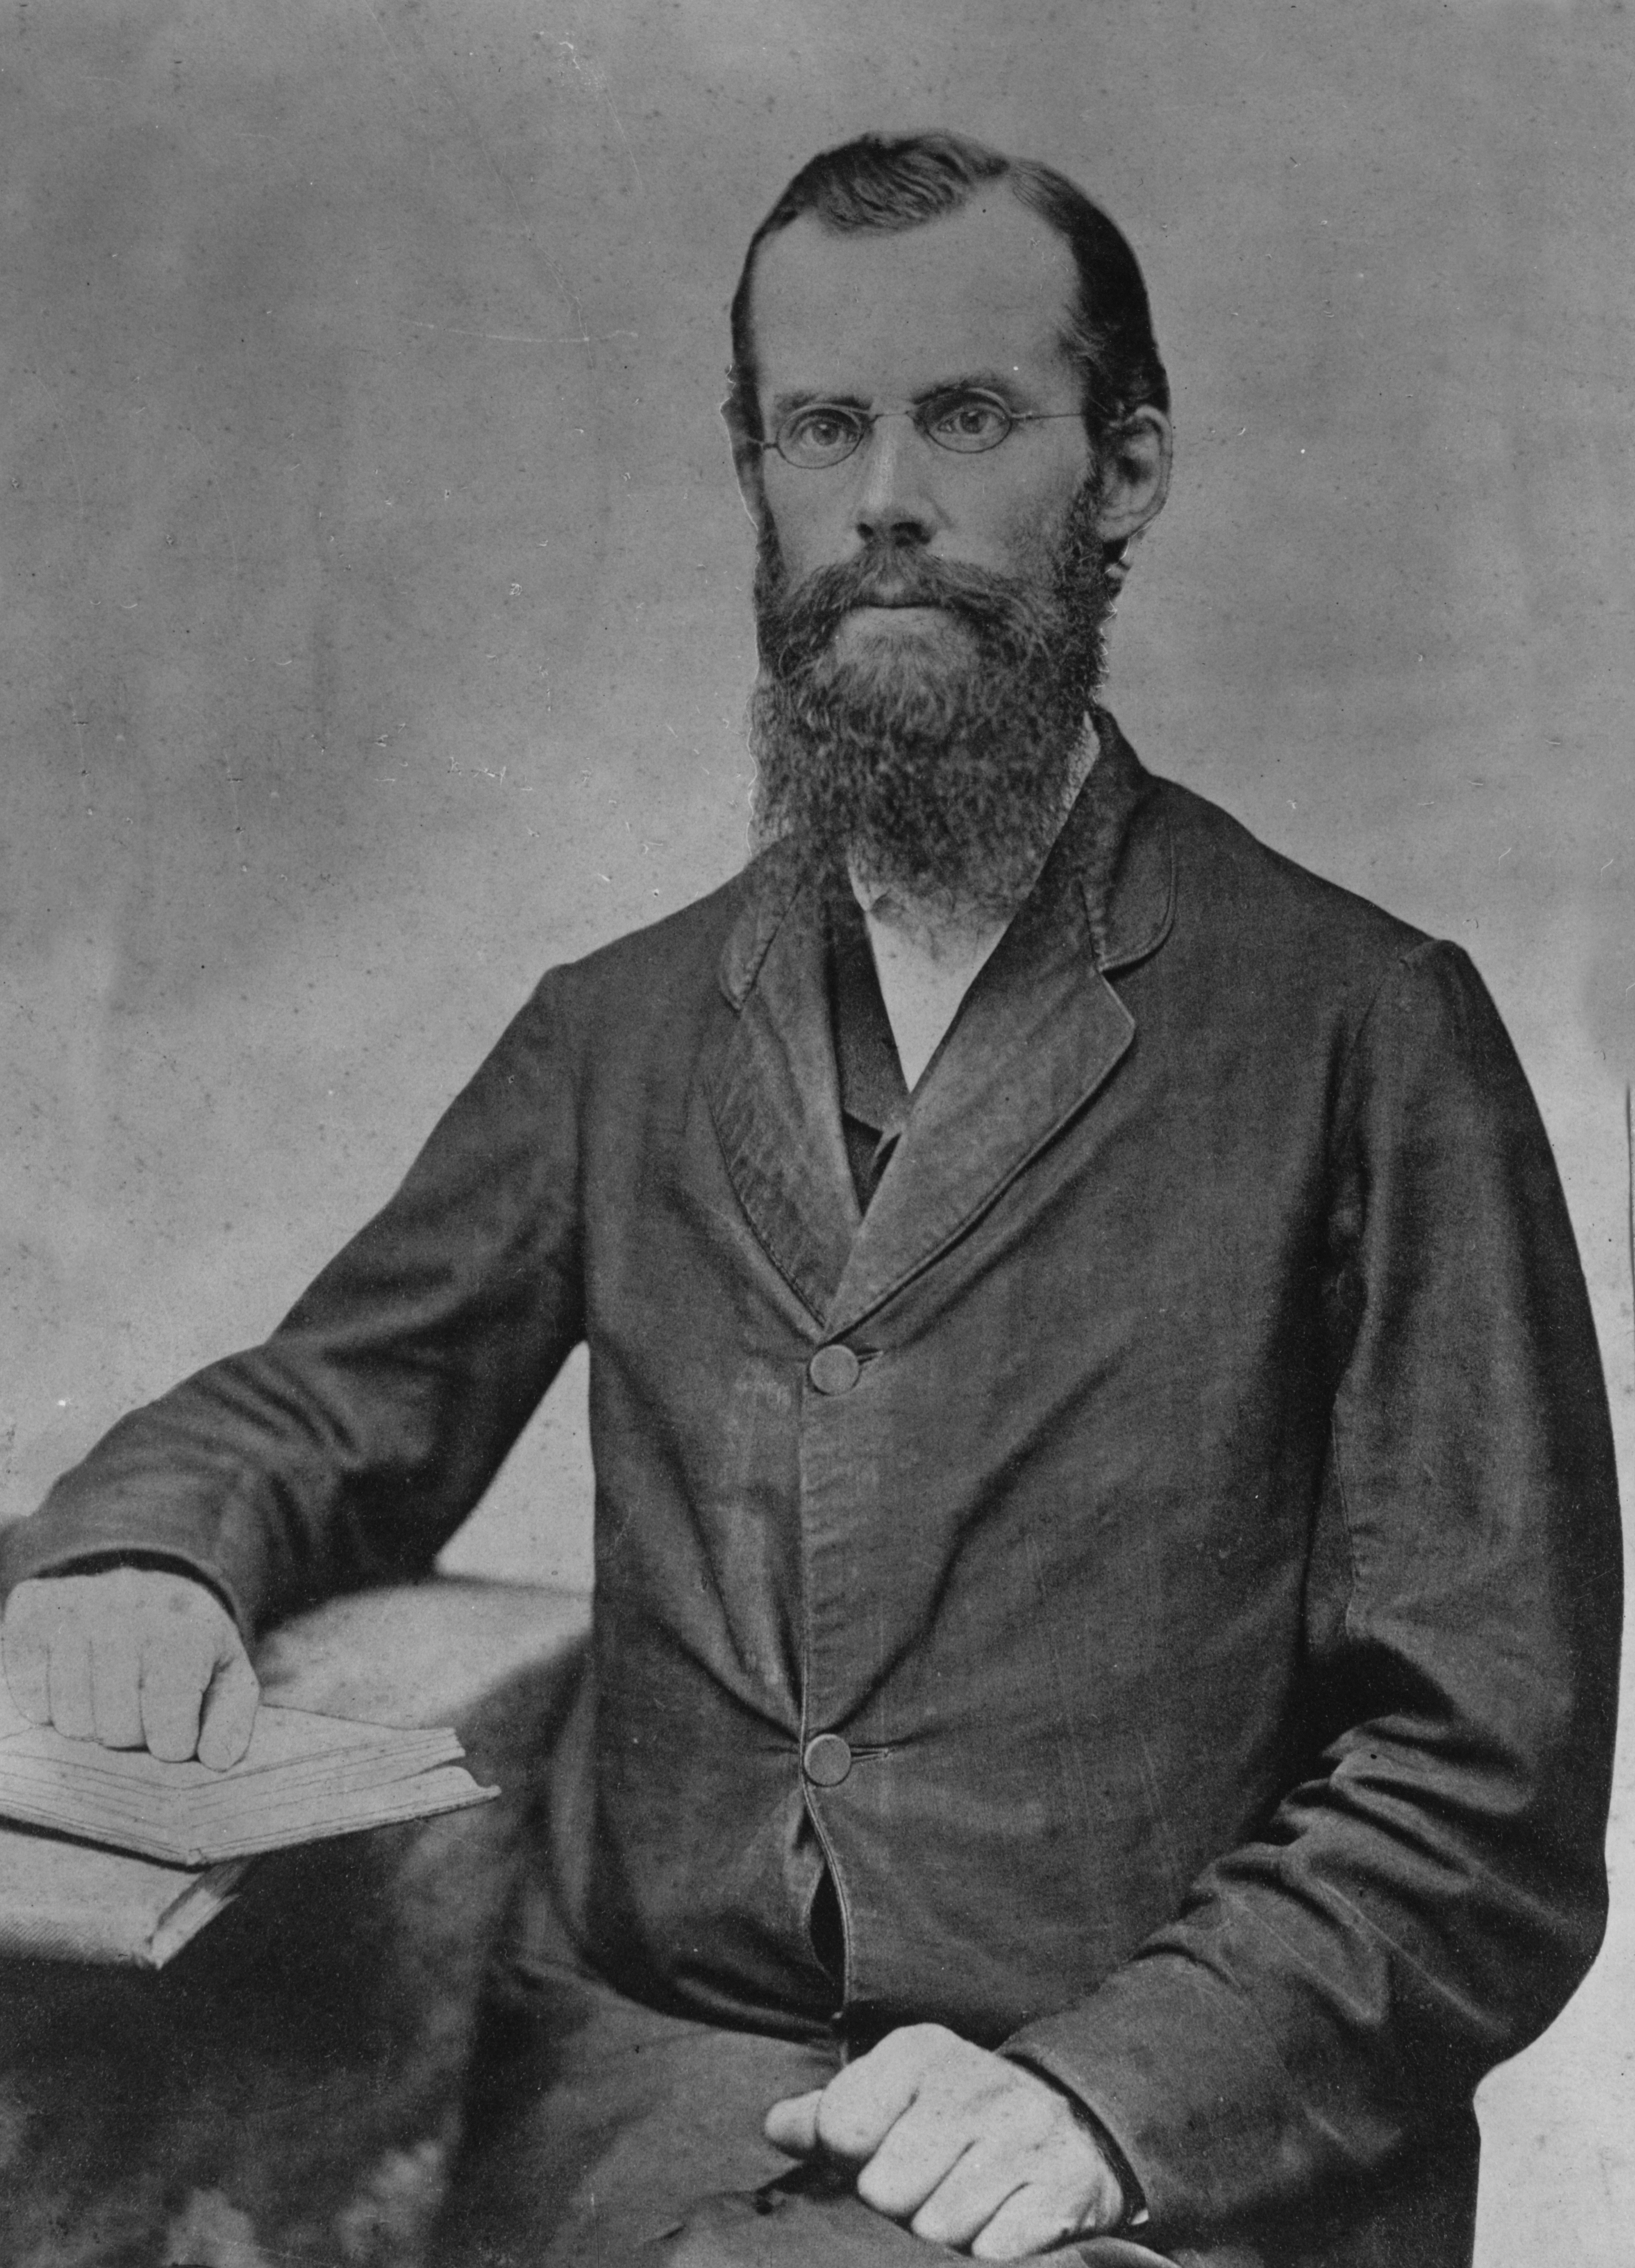
\includegraphics[width=1\linewidth]{images/john-nevins-andrews.jpg}
    \caption*{John Nevins Andrews (1829-1883)}
    \label{fig:j-n-andrews}
\end{figure}


\begin{figure}[hp]
    \centering
    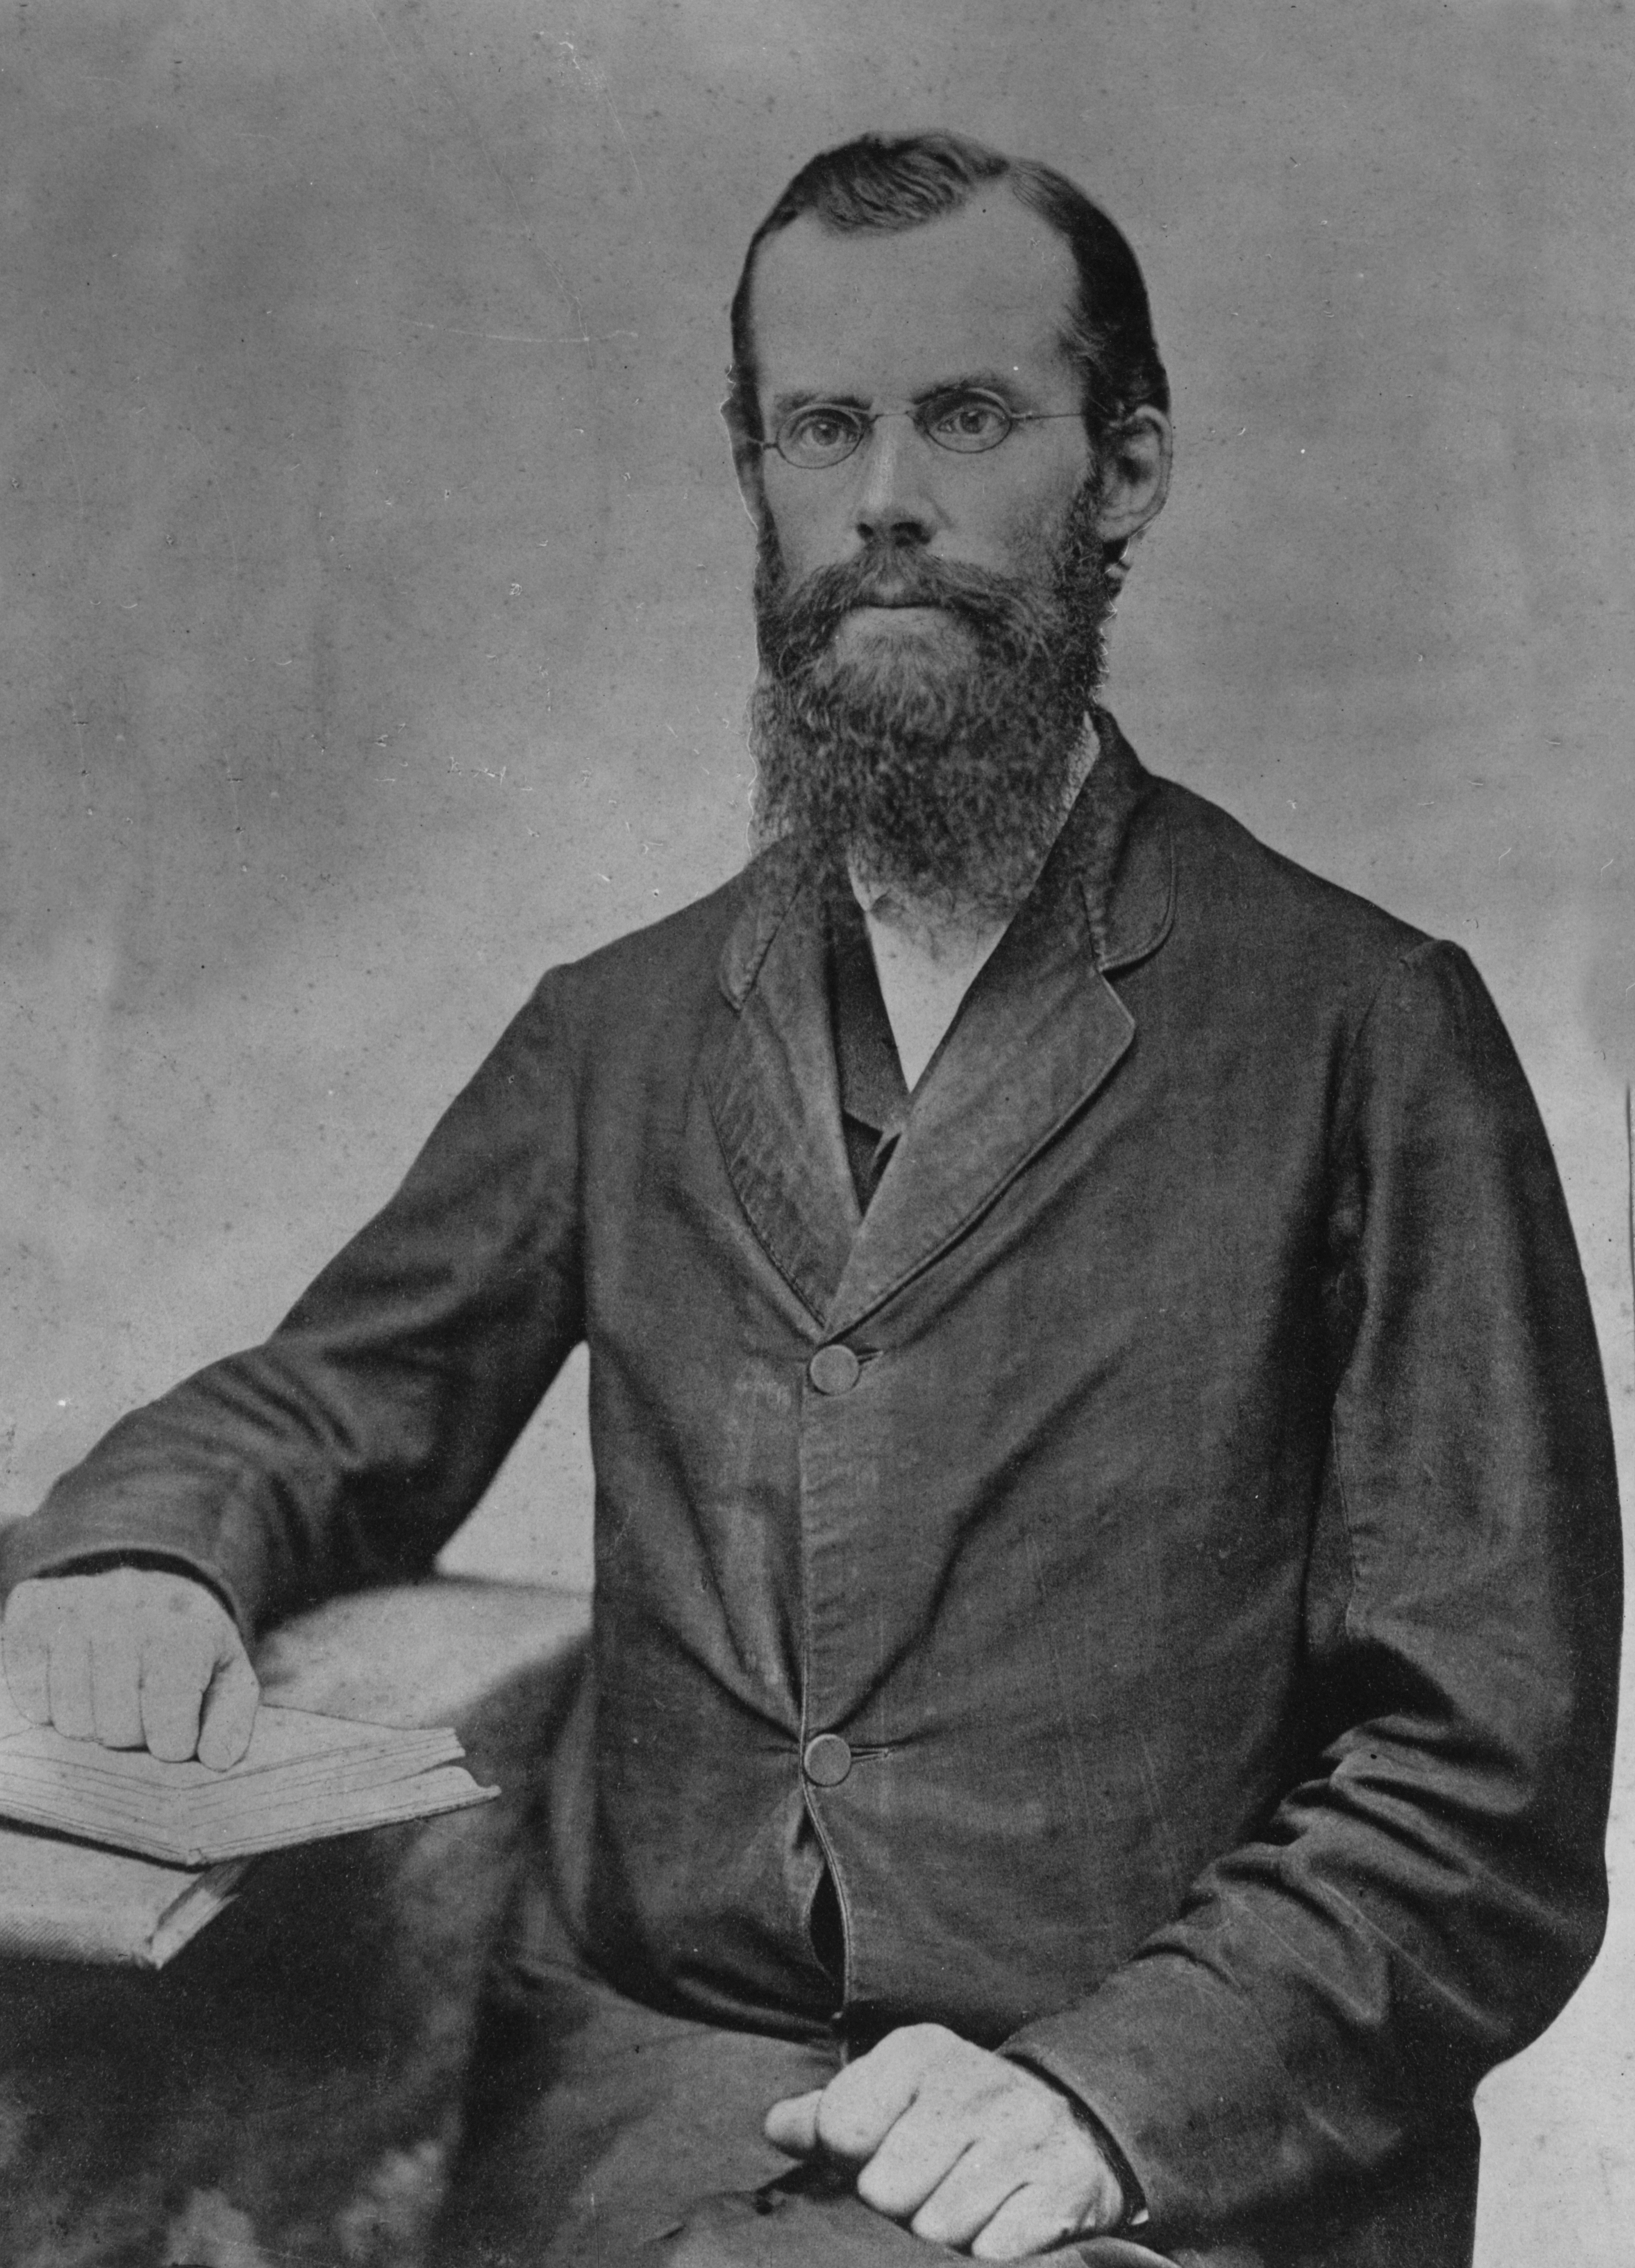
\includegraphics[width=1\linewidth]{images/john-nevins-andrews.jpg}
    \caption*{John Nevins Andrews (1829-1883)}
    \label{fig:j-n-andrews}
\end{figure}


J. N. Andrews said, \others{\textbf{The doctrine of the Trinity which was established in the church by the council of Nicea, A. D. 325}. \textbf{This doctrine \underline{destroys the personality of God, and his Son Jesus Christ our Lord}}...}[John. N. Andrews, The Advent Review and Sabbath Herald, March 6, 1855, p. 185][http://documents.adventistarchives.org/Periodicals/RH/RH18550306-V06-24.pdf]


J. N. Andrews dijo, \others{\textbf{La doctrina de la trinidad que fue establecida en la iglesia por el concilio de Nicea, el año 325 d.C.}. \textbf{Esta doctrina \underline{destruye la personalidad de Dios, y de su Hijo Jesucristo nuestro Señor}}...}[John. N. Andrews, The Advent Review and Sabbath Herald, March 6, 1855, p. 185][http://documents.adventistarchives.org/Periodicals/RH/RH18550306-V06-24.pdf]


In the context of the trinitarian understanding of the \emcap{personality of God}, it is safe to say that the \emcap{personality of God}, or the quality or state of God being a person, in any understanding of Trinity doctrine is a mystery. The problem is that there is no clear view of who is that \textit{one God} who is a person? The underlying claim is made that God is One yet Three, or One in Three; yes, God is a person, and He is one, yet simultaneously He is three persons. This view can never hold any clear perception of the \emcap{personality of God}. Also, it will deny the clearest testimony of the Scriptures that the one God is the Father, and that Christ is truly His only begotten Son. Most trinitarian brothers would agree that Christ is a real and definite being but if a trinitarian were to accept the Father as a real and definite Being, he would also need to accept the Holy Spirit as a real and definite being, thus denying the Holy Spirit as being a \textit{spirit}, the means by which the Father and Son are omnipresent. Conversely, if a trinitarian accepted the Holy Spirit to be a literal spirit, having no body nor form, then he would deny the Father to be a real, definite being. In conversation over the quality or state of God being a person, there is never a clear view of the matter with promoters of the Trinity doctrine; it is subterfuge. \textit{‘Subterfuges’} is a word Sister White used to describe the deception by artifice or stratagem in order to conceal, escape, or evade\footnote{\href{https://www.merriam-webster.com/dictionary/subterfuges}{The Merriam-Webster, ‘subterfuges’} - “\textit{deception by artifice or stratagem in order to conceal, escape, or evade}”} the truth; in other words, something that you cannot grab by head or tail. This is the primary reason Sister White did not engage in the Trinity discussion that would come up in the Seventh-day Adventist Church.


En el contexto de la comprensión trinitaria de la \emcap{personalidad de Dios}, es seguro decir que la \emcap{personalidad de Dios}, o la cualidad o estado de Dios siendo una persona, en cualquier comprensión de la doctrina trinitaria es un misterio. El problema es que no hay una visión clara de quién es ese \textit{un Dios} que es una persona. La afirmación subyacente es que Dios es Uno y a la vez Tres, o Uno en Tres; sí, Dios es una persona, y es uno, pero simultáneamente es tres personas. Este punto de vista nunca puede sostener ninguna percepción clara de la \emcap{personalidad de Dios}. Además, negará el testimonio más claro de las Escrituras de que el único Dios es el Padre, y que Cristo es verdaderamente su Hijo unigénito. La mayoría de los hermanos trinitarios estarían de acuerdo en que Cristo es un ser real y definido, pero si un trinitario aceptara al Padre como un Ser real y definido, también tendría que aceptar al Espíritu Santo como un ser real y definido, negando así que el Espíritu Santo sea un \textit{espíritu}, el medio por el cual el Padre y el Hijo son omnipresentes. Por el contrario, si un trinitario aceptara que el Espíritu Santo es un espíritu literal, que no tiene cuerpo ni forma, entonces negaría que el Padre sea un ser real y definido. En la conversación sobre la cualidad o estado de Dios siendo una persona, nunca hay una visión clara del asunto con los promotores de la doctrina trinitaria; es un subterfugio. \textit{‘Subterfugios’} es una palabra que la hermana White utilizó para describir el engaño por medio de artificios o estratagemas con el fin de ocultar, escapar o evadir\footnote{\href{https://www.merriam-webster.com/dictionary/subterfuges}{The Merriam-Webster, ‘subterfuges’} - “\textit{deception by artifice or stratagem in order to conceal, escape, or evade}”} la verdad; en otras palabras, algo que no se puede agarrar por la cabeza o la cola. Esta es la razón principal por la que la hermana White no se involucró en la discusión sobre la Trinidad que surgiría en la Iglesia Adventista del Séptimo Día.


\egw{I was cautioned not to enter into controversy \textbf{regarding the question} that \textbf{\underline{will come up}} over \textbf{these things, because controversy \underline{might lead men to resort to subterfuges, and their minds would be led away from the truth of the Word of God to assumption and guesswork}}. \textbf{The more that fanciful theories are discussed, the \underline{less men will know of God and of the truth that sanctifies the soul}}.}[Lt232-1903.41; 1903][https://egwwritings.org/read?panels=p10197.50]


\egw{Se me advirtió que no entrara en controversia \textbf{respecto a la cuestión} que \textbf{\underline{surgirá}} sobre \textbf{estas cosas, porque la controversia \underline{podría llevar a los hombres a recurrir a subterfugios, y sus mentes serían desviadas de la verdad de la Palabra de Dios hacia suposiciones y conjeturas}}. \textbf{Cuanto más se discutan las teorías extravagantes, \underline{menos conocerán los hombres a Dios y a la verdad que santifica el alma}}.}[Lt232-1903.41; 1903][https://egwwritings.org/read?panels=p10197.50]


When we read the works of Seventh-day Adventist pioneers on the \emcap{personality of God}, we see that they did not fall into the Trinity trap. Their non-trinitarian views of God were not due to ignorance, but a knowledge of the truth on the \emcap{personality of God}. They were of keen and noble intellect, understanding the thin line between the truth and error. Their understanding of the \emcap{personality of God} is balanced and solid, strongly supported by the plain and simple “\textit{thus says the Lord}”.


Cuando leemos las obras de los pioneros adventistas del séptimo día sobre la \emcap{personalidad de Dios}, vemos que no cayeron en la trampa de la Trinidad. Sus puntos de vista no trinitarios sobre Dios no se debían a la ignorancia, sino al conocimiento de la verdad sobre la \emcap{personalidad de Dios}. Eran de intelecto agudo y noble, comprendiendo la delgada línea entre la verdad y el error. Su comprensión de la \emcap{personalidad de Dios} es equilibrada y sólida, fuertemente apoyada por el liso y llano “\textit{así dice el Señor}”.


Many Adventists today accept the Trinity doctrine because Ellen White supposedly accepted it and promoted it. This is far from the truth and such a conclusion is predicated on lacking knowledge of the Spirit of Prophecy. If anyone was acquainted with the beliefs of Sister White, it was her husband James White. Here is what he has to say about the writings of his wife:


Muchos adventistas de hoy aceptan la doctrina trinitaria porque supuestamente Ellen White la aceptó y la promovió. Esto está muy lejos de la verdad y tal conclusión se basa en la falta de conocimiento del Espíritu de Profecía. Si alguien conocía las creencias de la hermana White, era su esposo James White. Esto es lo que él tiene que decir sobre los escritos de su esposa:


\others{\textbf{We invite all to compare the testimonies of the Holy Spirit through Mrs. W., with the word of God}. \textbf{And in this we do not invite you to compare them \underline{with your creed}}. That is quite another thing. \textbf{\underline{The trinitarian may compare them with his creed, and because they do not agree with it, condemn them}}. The observer of Sunday, or the man who holds eternal torment an important truth, and the minister that sprinkles infants, may each condemn the testimonies’ of Mrs. W. because they do not agree with their peculiar views. And a hundred more, each holding different views, may come to the same conclusion. \textbf{But their genuineness can never be tested in this way}.}[James S. White, The Advent Review, and Herald of the Sabbath, June 13, 1871][https://documents.adventistarchives.org/Periodicals/RH/RH18710613-V37-26.pdf]


\others{\textbf{Invitamos a todos a comparar los testimonios del Espíritu Santo a través de la Sra. W., con la palabra de Dios}. \textbf{Y en esto no los invitamos a compararlos \underline{con su credo}}. Eso es otra cosa. \textbf{\underline{El trinitario puede compararlos con su credo, y por no estar de acuerdo con él, condenarlos}}. El observador del domingo, o el hombre que sostiene que el tormento eterno es una verdad importante, y el ministro que rocía a los bebés, pueden cada uno condenar los testimonios de la Sra. W. porque no están de acuerdo con sus puntos de vista peculiares. Y cien más, cada uno de los cuales sostiene diferentes puntos de vista, pueden llegar a la misma conclusión. \textbf{Pero su autenticidad nunca puede ser probada de esta manera}.}[James S. White, The Advent Review, and Herald of the Sabbath, June 13, 1871][https://documents.adventistarchives.org/Periodicals/RH/RH18710613-V37-26.pdf]


James White was the closest associate of Ellen White, the person who was one with her in God’s uplifting of the Seventh-day Adventist Church. We have a clear and direct testimony from him that Ellen White’s writings are not trinitarian. Today, scholars put a false narrative that Ellen White grew in her understanding of the Trinity doctrine, and eventually accepted and preached it. But we see that Ellen White did not change her standpoint on the \emcap{personality of God} nor did she adhere to the Trinity doctrine. She was unambiguous in her claim that she never did. When the Kellogg crisis came over the \emcap{personality of God}, she remained firm in her view, just as all early Seventh-day Adventist pioneers did—and her dealings with Dr. Kellogg prove that. It is true, the Trinity doctrine \textit{cannot be accepted by those who are loyal to the faith and to the principles that have withstood all the opposition of satanic influences}.\footnote{\egw{Patchwork theories cannot be accepted by those who are loyal to the faith and to the principles that have withstood all the opposition of satanic influences}[Lt253-1903.28; 1903][https://egwwritings.org/read?panels=p14068.9980036]} Today’s official narrative that Ellen White was teaching the Trinity echoes Dr. Kellogg’s claim that the Living Temple taught the same thing as Ellen White. \egwinline{\textbf{But God forbid that this sentiment should prevail}.}[SpTB02 53.3; 1904][https://egwwritings.org/read?panels=p417.272]


James White fue el asociado más cercano de Ellen White, la persona que fue uno con ella en la elevación de la Iglesia Adventista del Séptimo Día por parte de Dios. Tenemos un testimonio claro y directo de él de que los escritos de Ellen White no son trinitarios. Hoy en día, los académicos ponen una narrativa falsa de que Ellen White creció en su comprensión de la doctrina trinitaria, y finalmente la aceptó y la predicó. Pero vemos que Ellen White no cambió su punto de vista sobre la \emcap{personalidad de Dios} ni se adhirió a la doctrina trinitaria. Fue inequívoca en su afirmación de que nunca lo hizo. Cuando se produjo la crisis de Kellogg sobre la \emcap{personalidad de Dios}, ella se mantuvo firme en su punto de vista, al igual que todos los primeros pioneros adventistas del séptimo día—y su trato con el Dr. Kellogg lo demuestra. Es cierto, la doctrina trinitaria \textit{no puede ser aceptada por aquellos que son leales a la fe y a los principios que han resistido toda la oposición de las influencias satánicas}.\footnote{\egw{Las teorías de parches no pueden ser aceptadas por aquellos que son leales a la fe y a los principios que han resistido toda la oposición de las influencias satánicas}[Lt253-1903.28; 1903][https://egwwritings.org/read?panels=p14068.9980036]} La narrativa oficial actual de que Ellen White enseñaba la Trinidad se hace eco de la afirmación del Dr. Kellogg de que The Living Temple enseñaba lo mismo que Ellen White. \egwinline{\textbf{Pero Dios no permita que este sentimiento prevalezca}.}[SpTB02 53.3; 1904][https://egwwritings.org/read?panels=p417.272]


% Adventist pioneers and the Trinity doctrine

\begin{titledpoem}
    \stanza{
        The pioneers stood firm against the Trinity's sway, \\
        Their testimony clear as the light of day. \\
        They saw how this doctrine did subtly disguise, \\
        What Scripture reveals to discerning eyes.
    }

    \stanza{
        James White declared it among "popular fables" found, \\
        A teaching that makes God's personality unsound. \\
        For Father and Son as distinct beings stand, \\
        Not merged into one as the Trinity planned.
    }

    \stanza{
        Two separate persons with purpose aligned, \\
        In spirit and action, united in mind. \\
        Just as disciples in Christ become one, \\
        Yet remain individual under God's Son.
    }

    \stanza{
        The Holy Spirit, God's presence divine, \\
        Not a separate being of the Godhead's design. \\
        But truly God's Spirit sent forth from above, \\
        The Father's representative, agent of love.
    }

    \stanza{
        No Scripture supports what tradition declared, \\
        When at Nicea this doctrine was shared. \\
        John seventeen shatters the trinitarian view, \\
        Revealing the Father and Son as beings true.
    }

    \stanza{
        Christ's divinity rests not in mysterious three, \\
        But in His begotten Sonship we see. \\
        The express image of His Father's face, \\
        Inheriting fullness of divine grace.
    }

    \stanza{
        The pioneers knew what the Bible made clear, \\
        That God is the Father, a Being most dear. \\
        A personal, spiritual presence on high, \\
        Omnipresent through Spirit, yet dwelling on high.
    }

    \stanza{
        So stands the truth against error's long night, \\
        Preserved by the pioneers and Sister White. \\
        Not through confusion or mystical thought, \\
        But through plain Scripture the truth has been taught.
    }
\end{titledpoem}


% Adventist pioneers and the Trinity doctrine

\begin{titledpoem}
    \stanza{
        The pioneers stood firm against the Trinity's sway, \\
        Their testimony clear as the light of day. \\
        They saw how this doctrine did subtly disguise, \\
        What Scripture reveals to discerning eyes.
    }

    \stanza{
        James White declared it among "popular fables" found, \\
        A teaching that makes God's personality unsound. \\
        For Father and Son as distinct beings stand, \\
        Not merged into one as the Trinity planned.
    }

    \stanza{
        Two separate persons with purpose aligned, \\
        In spirit and action, united in mind. \\
        Just as disciples in Christ become one, \\
        Yet remain individual under God's Son.
    }

    \stanza{
        The Holy Spirit, God's presence divine, \\
        Not a separate being of the Godhead's design. \\
        But truly God's Spirit sent forth from above, \\
        The Father's representative, agent of love.
    }

    \stanza{
        No Scripture supports what tradition declared, \\
        When at Nicea this doctrine was shared. \\
        John seventeen shatters the trinitarian view, \\
        Revealing the Father and Son as beings true.
    }

    \stanza{
        Christ's divinity rests not in mysterious three, \\
        But in His begotten Sonship we see. \\
        The express image of His Father's face, \\
        Inheriting fullness of divine grace.
    }

    \stanza{
        The pioneers knew what the Bible made clear, \\
        That God is the Father, a Being most dear. \\
        A personal, spiritual presence on high, \\
        Omnipresent through Spirit, yet dwelling on high.
    }

    \stanza{
        So stands the truth against error's long night, \\
        Preserved by the pioneers and Sister White. \\
        Not through confusion or mystical thought, \\
        But through plain Scripture the truth has been taught.
    }
\end{titledpoem}
          % Chapter 14
\qrchapter{https://forgottenpillar.com/rsc/en-fp-chapter15}{Dr. Kellogg and the Trinity doctrine}


\qrchapter{https://forgottenpillar.com/rsc/es-fp-chapter15}{Dr. Kellogg y la doctrina trinitaria}


The key problem with the Kellogg controversy was the sentiments over the \emcap{personality of God}, which were departing from the foundation of our faith, that God established at the beginning of our work. We have been told that \egwinline{Many things of like character will in the future arise}[Ms137-1903.10; 1903][https://egwwritings.org/read?panels=p9939.17]. In the book, the Living Temple, we see the sentiments regarding the \emcap{personality of God} and where His presence is, which were stepping off of the \emcap{Fundamental Principles}. This step was never supposed to be made! But we raise the question, where was this step heading? We will see the evidence that this step was heading toward the Trinity doctrine. Sister White prophesied that Kellogg’s step would lead toward the Omega heresy. Can we see the connection between Kellogg’s controversy and the Trinity doctrine?


El problema clave con la controversia de Kellogg fueron los sentimientos sobre la \emcap{personalidad de Dios}, que se apartaban del fundamento de nuestra fe, que Dios estableció al principio de nuestra obra. Se nos ha dicho que \egwinline{Muchas cosas de carácter similar surgirán en el futuro}[Ms137-1903.10; 1903][https://egwwritings.org/read?panels=p9939.17]. En el libro, The Living Temple, vemos los sentimientos con respecto a la \emcap{personalidad de Dios} y donde está Su presencia, que se estaban alejando de los \emcap{Principios Fundamentales}. ¡Este paso no debía darse nunca! Pero nos preguntamos, ¿hacia dónde se dirigía este paso? Veremos la evidencia de que este paso se dirigía hacia la doctrina trinitaria. La hermana White profetizó que el paso de Kellogg conduciría a la herejía Omega. ¿Podemos ver la conexión entre la controversia de Kellogg y la doctrina trinitaria?


In the following section, we want to present you with the connection between Kellogg’s controversy and the doctrine of Trinity. It is important to emphasize that the Living Temple does not contain this doctrine as it is believed today. The main problem with Kellogg’s teaching was the \textit{stepping off} of the \emcap{Fundamental Principles}, which were the foundation of our faith. The information we will present to you reveals that Dr. Kellogg justified his actions in stepping off of the foundation through his belief in the doctrine of Trinity. This is not difficult to see when we recognize that the \emcap{Fundamental Principles} were a non-Trinitarian. Our main focus should not be in recognizing the Trinity doctrine in Kellogg's arguments, but rather in understanding the differences between Kellogg’s teachings and the teachings of the \emcap{Fundamental Principles} regarding \egwinline{the personality of God and where His presence is}[SpTB02 51.3; 1903][https://egwwritings.org/read?panels=p417.262]. In other words, what were the steps Kellogg made in stepping off of the foundation of our faith? This approach is advocated by the Spirit of Prophecy and it will help us to avoid speculations regarding Kellogg’s motives—it will help us to focus upon the truth. Ellen White tells us that there are many good things written in the Living Temple, but they are mingled with specious, deceptive theories regarding the \emcap{personality of God} and \emcap{of Christ}.


En la siguiente sección, queremos presentarles la conexión entre la controversia de Kellogg y la doctrina trinitaria. Es importante enfatizar que el Living Temple no contiene esta doctrina como se cree hoy en día. El principal problema con la enseñanza de Kellogg fue el \textit{alejamiento} de los \emcap{Principios Fundamentales}, que eran la base de nuestra fe. La información que les presentaremos revela que el Dr. Kellogg justificó sus acciones al salirse del fundamento a través de su creencia en la doctrina trinitaria. Esto no es difícil de ver cuando reconocemos que los \emcap{Principios Fundamentales} eran no-trinitarios. Por lo tanto, nuestro enfoque principal no debe ser reconocer la doctrina trinitaria en los argumentos de Kellogg, sino más bien entender las diferencias entre las enseñanzas de Kellogg y las enseñanzas de los \emcap{Principios Fundamentales} con respecto a \egwinline{la personalidad de Dios y dónde está su presencia}[SpTB02 51.3; 1903][https://egwwritings.org/read?panels=p417.262]. En otras palabras, ¿cuáles fueron los pasos que dio Kellogg al salirse del fundamento de nuestra fe? Este enfoque es defendido por el Espíritu de Profecía y nos ayudará a evitar especulaciones sobre los motivos de Kellogg—nos ayudará a centrarnos en la verdad. Elena G. de White nos dice que hay muchas cosas buenas escritas en el Living Temple, pero están mezcladas con teorías engañosas y especiosas respecto a la \emcap{personalidad de Dios} y \emcap{de Cristo}.


\begin{figure}[hp]
    \centering
    \includegraphics[width=1\linewidth]{images/john-h-kellogg.jpg}
    \caption*{John Harvey Kellogg (1852-1943)}
    \label{fig:john-h-kellogg}
\end{figure}


\begin{figure}[hp]
    \centering
    \includegraphics[width=1\linewidth]{images/john-h-kellogg.jpg}
    \caption*{John Harvey Kellogg (1852-1943)}
    \label{fig:john-h-kellogg}
\end{figure}


\egw{\textbf{The book Living Temple contains specious, \underline{deceptive sentiments regarding the personality of God and of Christ}}. The Lord opened before me the true meaning of these sentiments, showing me that unless they were steadfastly repudiated, they would deceive the very elect. \textbf{Precious truth and beautiful sentiments were woven in with false, misleading theories. Thus truth was used to substantiate the \underline{most dangerous errors}. The precious representations of God are so misconstrued as to appear to uphold falsehoods \underline{originated by the great apostate}. Sentiments that belong to the revealings of God are mingled with specious, deceptive theories of satanic agencies}.}[Lt146-1905.2; 1905][https://egwwritings.org/read?panels=p9430.8]


\egw{\textbf{El libro Living Temple contiene sentimientos especiosos, \underline{engañosos respecto a la personalidad de Dios y de Cristo}}. El Señor abrió ante mí el verdadero significado de estos sentimientos, mostrándome que, a menos que fueran firmemente repudiados, engañarían a los mismos elegidos. \textbf{La preciosa verdad y los hermosos sentimientos se entretejían con teorías falsas y engañosas. Así, la verdad fue utilizada para fundamentar los \underline{errores más peligrosos}. Las preciosas representaciones de Dios se malinterpretan de tal manera que parecen sostener falsedades \underline{originadas por el gran apóstata}. Los sentimientos que pertenecen a las revelaciones de Dios se mezclan con teorías engañosas y especiosas de los organismos satánicos}.}[Lt146-1905.2; 1905][https://egwwritings.org/read?panels=p9430.8]


\egwnogap{In the controversy over these theories \textbf{it has been asserted that I believed and taught the same things} that I have been instructed to condemn in the book Living Temple. \textbf{This I deny}. In the name of Jesus Christ of Nazareth, \textbf{I say that this is not so}.}[Lt146-1905.3; 1905][https://egwwritings.org/read?panels=p9430.9]


\egwnogap{En la controversia sobre estas teorías \textbf{se ha afirmado que yo creía y enseñaba las mismas cosas} que se me ha ordenado condenar en el libro Living Temple. \textbf{Esto lo niego}. En nombre de Jesucristo de Nazaret, \textbf{digo que no es así}.}[Lt146-1905.3; 1905][https://egwwritings.org/read?panels=p9430.9]


This mixture of truth and error makes the matter difficult. In the eyes of pro-trinitarian scholars, the problem is solely attributed to pantheism, and the evidence of Kellogg's belief in the Trinity doctrine is interpreted as belief in a false Trinity\footnote{Whidden, Woodrow W, et al. \textit{The Trinity : Understanding God's Love, His Plan of Salvation, and Christian Relationships}. Hagerstown, Md, Review And Herald Pub. Association, 2002., p. 217}. Sister White's rebuke is attributed to the defense of the “correct” Trinity, which she supposedly believed. Unfortunately, such interpretation does not acknowledge Sister White's defense of the \emcap{Fundamental Principles} regarding the \emcap{personality of God} and of Christ, thus it is a misinterpretation of her work. In the following sections, we will examine historical data on Dr. Kellogg's connection with the doctrine of Trinity from the perspective of the Adventist truth on the \emcap{personality of God}, which constituted the foundation of our faith. With this perspective, we believe that the historical data will shine in a new light and spark honest and constructive dialogue in our church.


Esta mezcla de verdad y error dificulta el asunto. A los ojos de los académicos pro-trinitarios, el problema se atribuye únicamente al panteísmo, y la evidencia de la creencia de Kellogg en la doctrina trinitaria se interpreta como una creencia en una falsa trinidad\footnote{Whidden, Woodrow W, et al. \textit{The Trinity : Understanding God's Love, His Plan of Salvation, and Christian Relationships}. Hagerstown, Md, Review And Herald Pub. Association, 2002., p. 217}. La reprimenda de la hermana White se atribuye a la defensa de la trinidad “correcta”, en la que supuestamente creía. Desgraciadamente, tal interpretación no reconoce la defensa de la hermana White de los \emcap{Principios Fundamentales} respecto a la \emcap{personalidad de Dios} y de Cristo, por lo que es una interpretación errónea de su obra. En las siguientes secciones, examinaremos los datos históricos sobre la conexión del Dr. Kellogg con la doctrina trinitaria desde la perspectiva de la verdad adventista sobre la \emcap{personalidad de Dios}, que constituyó el fundamento de nuestra fe. Con esta perspectiva, creemos que los datos históricos brillarán con una nueva luz y provocarán un diálogo honesto y constructivo en nuestra iglesia.


\section*{Correspondence of Dr. Kellogg and Brother Butler}


\section*{Correspondencia del Dr. Kellogg y el hermano Butler}


In the following section we briefly present you with the well-known correspondence between Dr. Kellogg and G. I. Butler over the book, the Living Temple. Here, we see Dr. Kellogg’s objections regarding the controversy. He wrote to Brother Butler:


En la siguiente sección les presentamos brevemente la conocida correspondencia entre el Dr. Kellogg y G. I. Butler sobre el libro, el Living Temple. Aquí vemos las objeciones del Dr. Kellogg con respecto a la controversia. Escribió al hermano Butler:


\others{As far as I can fathom, the \textbf{difficulty }which is found \textbf{in ‘The Living Temple’,} \textbf{the whole thing may be simmered down to the question}: \textbf{\underline{Is the Holy Ghost a person}?} You say no. I had supposed the Bible said this for the reason that the personal pronoun ‘he’ is used in speaking of the Holy Ghost. \textbf{Sister White uses the pronoun ‘he’ and has said in so many words that the Holy Ghost is \underline{the third person of the Godhead}}. \textbf{How the Holy Ghost can be the third person and not be a person at all is difficult for me to see}.}[Letter: J. H. Kellogg to G. I. Butler. Oct 28. 1903][https://static1.squarespace.com/static/554c4998e4b04e89ea0c4073/t/5db9fbc96defed1e45b497a4/1572469707862/1903-10-28-Kellog-to-Butler.pdf]


\others{Hasta donde puedo entender, la \textbf{dificultad} que se encuentra \textbf{en ‘The Living Temple’,} \textbf{todo el asunto puede reducirse a la pregunta}: \textbf{\underline{¿Es el Espíritu Santo una persona}?} Usted dice que no. Yo había supuesto que la Biblia decía esto por la razón de que el pronombre personal ‘él’ se utiliza al hablar del Espíritu Santo. \textbf{La hermana White usa el pronombre ‘él’ y ha dicho en muchas palabras que el Espíritu Santo es \underline{la tercera persona de la Divinidad}}. \textbf{Cómo el Espíritu Santo puede ser la tercera persona y no ser una persona en absoluto me resulta difícil de ver}.}[Letter: J. H. Kellogg to G. I. Butler. Oct 28. 1903][https://static1.squarespace.com/static/554c4998e4b04e89ea0c4073/t/5db9fbc96defed1e45b497a4/1572469707862/1903-10-28-Kellog-to-Butler.pdf]


\begin{figure}[hp]
    \centering
    \includegraphics[width=1\linewidth]{images/george-ide-butler.jpg}
    \caption*{George Ide Butler (1834-1918)}
    \label{fig:g-i-butler}
\end{figure}


\begin{figure}[hp]
    \centering
    \includegraphics[width=1\linewidth]{images/george-ide-butler.jpg}
    \caption*{George Ide Butler (1834-1918)}
    \label{fig:g-i-butler}
\end{figure}


According to Dr. Kellogg’s perspective, the whole problem with the book ‘The Living Temple’ comes down to the question “\textit{Is the Holy Ghost a person?}”. Obviously, he does not advocate an impersonal God, as he is often accused of\footnote{Whidden, Woodrow W, et al. \textit{The Trinity : Understanding God's Love, His Plan of Salvation, and Christian Relationships}. Hagerstown, Md, Review And Herald Pub. Association, 2002., p. 217}. Moreover, he even believes that the Holy Ghost is a \textit{third person of the Godhead}. Also, he claims that Brother Butler does not believe that the Holy Ghost is a person. The problem obviously lies in the definition of the word \textit{‘person’}. On this point, Kellogg continues:


Según la perspectiva del Dr. Kellogg, todo el problema del libro ‘El Templo Viviente’ se reduce a la pregunta “\textit{¿Es el Espíritu Santo una persona?}”. Obviamente, él no defiende un Dios impersonal, como se le acusa a menudo\footnote{Whidden, Woodrow W, et al. \textit{The Trinity : Understanding God's Love, His Plan of Salvation, and Christian Relationships}. Hagerstown, Md, Review And Herald Pub. Association, 2002., p. 217}. Es más, incluso cree que el Espíritu Santo es una \textit{tercera persona de la Divinidad}. Además, afirma que el hermano Butler no cree que el Espíritu Santo sea una persona. El problema radica obviamente en la definición de la palabra \textit{‘persona’}. Sobre este punto, Kellogg continúa:


\others{I believe this Spirit of God to be a personality you don’t. But this is purely a question of definition. \textbf{I believe the Spirit of God is a personality}; you say, No, it is not a personality. Now the only reason why we differ is because we \textbf{differ in our ideas as to \underline{what a personality is}}. \textbf{Your idea of personality is perhaps that of \underline{semblance to a person} or a human being}.}[Letter: J. H. Kellogg to G. I. Butler. Oct 28. 1903][https://static1.squarespace.com/static/554c4998e4b04e89ea0c4073/t/5db9fbc96defed1e45b497a4/1572469707862/1903-10-28-Kellog-to-Butler.pdf]


\others{Yo creo que este Espíritu de Dios es una personalidad que tú no crees. Pero esto es puramente una cuestión de definición. \textbf{Yo creo que el Espíritu de Dios es una personalidad}; tú dices que no, que no es una personalidad. Ahora, la única razón por la que diferimos es porque \textbf{diferimos en nuestras ideas sobre \underline{lo que es una personalidad}}. \textbf{Tu idea de personalidad es quizás la de \underline{apariencia de una persona} o un ser humano}.}[Letter: J. H. Kellogg to G. I. Butler. Oct 28. 1903][https://static1.squarespace.com/static/554c4998e4b04e89ea0c4073/t/5db9fbc96defed1e45b497a4/1572469707862/1903-10-28-Kellog-to-Butler.pdf]


Brother Butler replied:


El hermano Butler respondió:


\others{\textbf{So far as Sister White and you being in perfect agreement, I shall have to leave that entirely between you and Sister White. \underline{Sister White says there is not perfect agreement; you claim there is}. \underline{I know some of her remarks seem to give you strong ground for claiming that she does}. I am candid enough to say that, but I must give her the credit until she disowns it of saying there is a difference too, and I do not believe you can fully tell just what she means. \underline{God dwells in us by His Holy Spirit}, as a Comforter, as a Reprover, especially the former. When we come to Him we partake of Him in that sense, because the Spirit comes forth from Him; \underline{it comes forth from the Father and the Son}. It is not a person walking around on foot, or flying \underline{as a literal being}, \underline{in any such sense as Christ and the Father are} – at least, if it is, it is utterly beyond my comprehension of the meaning of language or words}.}[Letter: G. I. Butler to J. H. Kellogg. April 5. 1904]


\others{\textbf{En cuanto a que la hermana White y usted estén en perfecto acuerdo, tendré que dejar eso totalmente entre usted y la hermana White. \underline{La hermana White dice que no hay un acuerdo perfecto; usted afirma que sí lo hay}. \underline{Sé que algunos de sus comentarios parecen darle a usted una base sólida para afirmar que sí lo hay}. Soy lo suficientemente sincero como para decir eso, pero debo darle el crédito, hasta que ella lo desmienta, de decir que también hay una diferencia, y no creo que usted pueda decir completamente lo que ella quiere decir. \underline{Dios mora en nosotros por medio de su Espíritu Santo}, como Consolador, como Reprobador, especialmente el primero. Cuando venimos a Él, participamos de Él en ese sentido, porque el Espíritu sale de Él; \underline{sale del Padre y del Hijo}. No es una persona que camina a pie, o que vuela \underline{como un ser literal}, \underline{en ningún sentido como lo son Cristo y el Padre} – al menos, si lo es, está totalmente más allá de mi comprensión del significado del lenguaje o palabras}.}[Letter: G. I. Butler to J. H. Kellogg. April 5. 1904]


The given correspondence is crucial for understanding the Kellogg controversy. Kellogg himself stated, \others{the whole thing may be simmered down to the question: \textbf{Is the Holy Ghost a person?}} Similarly Dr. Kellogg wrote to William White: \others{I have been studying very carefully to see what is \textbf{the real root of the difficulty with the Living Temple}, and as far as I can see \textbf{\underline{the whole question} resolves itself into this: \underline{Is the Holy Ghost, a person}?}}[Letter J. H. Kellogg to William White, October 28, 1903][https://drive.google.com/file/d/1\_S4S-Hc0K7Ka8gda9oRhPuAb9XzBTwmb/view] How does Kellogg's conclusion compare to the review and instruction of heavenly origin, which clearly told us that the reasoning in the Living Temple is \egwinline{naught but speculation in regard to \textbf{the personality of God and where His presence is}}[SpTB02 51.3; 1904][https://egwwritings.org/read?panels=p417.262]? In the writings of Ellen White and the pioneers, the term ‘\textit{personality of God}’ refers specifically to the personality of the Father. So, why does Kellogg claim that the real issue is the personality of the Holy Spirit, when God indicated that the issue concerns the personality of the Father?


La correspondencia dada es crucial para entender la controversia de Kellogg. El mismo Kellogg declaró, \others{todo el asunto puede reducirse a la pregunta: \textbf{¿Es el Espíritu Santo una persona?}} De manera similar, el Dr. Kellogg escribió a William White: \others{He estado estudiando muy cuidadosamente para ver cuál es \textbf{la verdadera raíz de la dificultad con el Templo Viviente}, y hasta donde puedo ver \textbf{\underline{toda la cuestión} se reduce a esto: \underline{¿Es el Espíritu Santo una persona}?}}[Letter J. H. Kellogg to William White, October 28, 1903][https://drive.google.com/file/d/1\_S4S-Hc0K7Ka8gda9oRhPuAb9XzBTwmb/view] ¿Cómo se compara la conclusión de Kellogg con la revisión e instrucción de origen celestial, que claramente nos dijo que el razonamiento en el Templo Viviente es \egwinline{nada más que especulación con respecto a \textbf{la personalidad de Dios y dónde está Su presencia}}[SpTB02 51.3; 1904][https://egwwritings.org/read?panels=p417.262]? En los escritos de Elena de White y los pioneros, el término ‘\textit{personalidad de Dios}’ se refiere específicamente a la personalidad del Padre. Entonces, ¿por qué Kellogg afirma que el verdadero problema es la personalidad del Espíritu Santo, cuando Dios indicó que el problema concierne a la personalidad del Padre?


Many assume that Dr. Kellogg is being manipulative, evading the core issue. However, under a particular premise, his arguments concerning the personality of the Holy Spirit logically support his controversial views on the \emcap{personality of God}. This premise becomes evident within the data itself when we closely follow his reasoning.


Muchos asumen que el Dr. Kellogg está siendo manipulador, evadiendo el problema central. Sin embargo, bajo una premisa particular, sus argumentos concernientes a la personalidad del Espíritu Santo apoyan lógicamente sus controvertidas opiniones sobre la \emcap{personalidad de Dios}. Esta premisa se hace evidente dentro de los datos mismos cuando seguimos de cerca su razonamiento.


As we have seen earlier, the doctrine on the \emcap{personality of God} teaches that God, the Father, possesses a form—a tangible, material body. Dr. Kellogg concurred that this assertion holds true within the bounds of our finite conception of God\footnote{\href{https://archive.org/details/J.H.Kellogg.TheLivingTemple1903/page/n33/}{Dr. John H. Kellogg, The Living Temple, p.31.}}. However, he argued that, in reality, God transcends our conceptions regarding His form, as He is beyond the constraints of space\footnote{\href{https://archive.org/details/J.H.Kellogg.TheLivingTemple1903/page/n33/}{Dr. John H. Kellogg, The Living Temple, p.33.}}. In this sense, Kellogg effectively does away with the reality of God’s physical, material body. The premise that would validate Dr. Kellogg’s viewpoint is the \textit{exclusive equivalence} in understanding the \emcap{personality of God} and that of the Holy Spirit. Is the Holy Spirit constrained by space? No, He is not. Does the Holy Spirit have a physical body? No! According to Jesus, \bible{for a spirit hath not flesh and bones}[Luke 24:39]. Is the Holy Ghost a person? The answer hinges on our interpretation of what it means to be a person. What is that quality or state of the Holy Spirit being a person?\footnote{Direct application of the definition on the word ‘\textit{personality}’ from the \href{https://www.merriam-webster.com/dictionary/personality}{Merriam Webster Dictionary}} When comparing Dr. Kellogg's belief in the personality of the Holy Spirit with Brother Butler's views, it becomes evident that the quality of the Holy Spirit being a person does not align with \others{that of \textbf{semblance to a person} or a human being}. Butler explicitly stated his criteria for this determination\footnote{In his letter to Dr. Kellogg, Brother Butler further asserted that there is no distinction between the person and the bodily presence. See \href{https://c7da.us/egwdl/Butler\%20to\%20Kellogg\%20Aug121904.pdf}{Letter from Butler to Kellogg, August 12, 1904, p.6}}: \others{\textbf{It is not a person walking around on foot, or flying \underline{as a literal being}, \underline{in any such sense as Christ and the Father are} – at least, if it is, it is utterly beyond my comprehension of the meaning of language or words}}.


Como hemos visto anteriormente, la doctrina sobre la \emcap{personalidad de Dios} enseña que Dios, el Padre, posee una forma—un cuerpo tangible y material. El Dr. Kellogg coincidió en que esta afirmación es válida dentro de los límites de nuestra concepción finita de Dios\footnote{\href{https://archive.org/details/J.H.Kellogg.TheLivingTemple1903/page/n33/}{Dr. John H. Kellogg, The Living Temple, p.31.}}. Sin embargo, argumentó que, en realidad, Dios trasciende nuestras concepciones respecto a Su forma, ya que está más allá de las limitaciones del espacio\footnote{\href{https://archive.org/details/J.H.Kellogg.TheLivingTemple1903/page/n33/}{Dr. John H. Kellogg, The Living Temple, p.33.}}. En este sentido, Kellogg efectivamente elimina la realidad del cuerpo físico y material de Dios. La premisa que validaría el punto de vista del Dr. Kellogg es la \textit{equivalencia exclusiva} en la comprensión de la \emcap{personalidad de Dios} y la del Espíritu Santo. ¿Está el Espíritu Santo limitado por el espacio? No, no lo está. ¿Tiene el Espíritu Santo un cuerpo físico? ¡No! Según Jesús, \bible{porque un espíritu no tiene carne ni huesos}[Lucas 24:39]. ¿Es el Espíritu Santo una persona? La respuesta depende de nuestra interpretación de lo que significa ser una persona. ¿Cuál es esa cualidad o estado del Espíritu Santo siendo una persona?\footnote{Aplicación directa de la definición de la palabra ‘\textit{personalidad}’ del \href{https://www.merriam-webster.com/dictionary/personality}{Diccionario Merriam Webster}} Al comparar la creencia del Dr. Kellogg en la personalidad del Espíritu Santo con las opiniones del hermano Butler, se hace evidente que la cualidad del Espíritu Santo siendo una persona no se alinea con \others{la de \textbf{apariencia de una persona} o un ser humano}. Butler declaró explícitamente sus criterios para esta determinación\footnote{En su carta al Dr. Kellogg, el hermano Butler afirmó además que no hay distinción entre la persona y la presencia corporal. Ver \href{https://c7da.us/egwdl/Butler\%20to\%20Kellogg\%20Aug121904.pdf}{Carta de Butler a Kellogg, 12 de agosto de 1904, p.6}}: \others{\textbf{No es una persona que camina a pie, o que vuela \underline{como un ser literal}, \underline{en ningún sentido como lo son Cristo y el Padre} – al menos, si lo es, está totalmente más allá de mi comprensión del significado del lenguaje o palabras}}.


Have you noticed that Brother Butler addressed Kellogg’s unspoken premise? Butler drew a distinction between the Father and Christ, in relation to the Holy Spirit. Brother Butler is correct. There exists a contrast between the personality of the Holy Spirit and that of God and Christ. Christ and the Father possess a physical form of a person, whereas the Holy Spirit does not. To do away with the physical form of a person of the Father is to \textit{exclusively equate} the understanding of the personality of the Father with that of the Holy Spirit. Kellogg’s approach is compelling, because it was backed by valid arguments regarding the personality of the Holy Spirit.


¿Has notado que el hermano Butler abordó la premisa no expresada de Kellogg? Butler estableció una distinción entre el Padre y Cristo, en relación con el Espíritu Santo. El hermano Butler tiene razón. Existe un contraste entre la personalidad del Espíritu Santo y la de Dios y Cristo. Cristo y el Padre poseen una forma física de persona, mientras que el Espíritu Santo no. Eliminar la forma física de la persona del Padre es \textit{equiparar exclusivamente} la comprensión de la personalidad del Padre con la del Espíritu Santo. El enfoque de Kellogg es convincente, porque estaba respaldado por argumentos válidos sobre la personalidad del Espíritu Santo.


Let us briefly examine the personality of the Holy Spirit. What is the quality or state of the Holy Spirit being a person?


Examinemos brevemente la personalidad del Espíritu Santo. ¿Cuál es la cualidad o estado del Espíritu Santo siendo una persona?


\egw{\textbf{The Holy Spirit has a personality}, \textbf{\underline{else} }He could not \textbf{bear witness} to our spirits and with our spirits that we are the children of God. \textbf{He must also be a \underline{divine person}}, \textbf{\underline{else}} He could not \textbf{search out the secrets} which lie hidden \textbf{in the mind of God}.}[21LtMs, Ms 20, 1906, par. 32; 1906][https://egwwritings.org/read?panels=p14071.10296041&index=0]


\egw{\textbf{El Espíritu Santo tiene una personalidad}, \textbf{\underline{de lo contrario} }no podría \textbf{dar testimonio} a nuestros espíritus y con nuestros espíritus de que somos hijos de Dios. \textbf{También debe ser una \underline{persona divina}}, \textbf{\underline{de lo contrario}} no podría \textbf{escudriñar los secretos} que están ocultos \textbf{en la mente de Dios}.}[21LtMs, Ms 20, 1906, par. 32; 1906][https://egwwritings.org/read?panels=p14071.10296041&index=0]


\egw{\textbf{The Holy Spirit is a person}; \textbf{\underline{for}} He \textbf{beareth witness} with our spirits that we are the children of God.}[21LtMs, Ms 20, 1906, par. 31; 1906][https://egwwritings.org/read?panels=p14071.10296040&index=0]


\egw{\textbf{El Espíritu Santo es una persona}; \textbf{\underline{porque}} Él \textbf{da testimonio} con nuestros espíritus de que somos hijos de Dios.}[21LtMs, Ms 20, 1906, par. 31; 1906][https://egwwritings.org/read?panels=p14071.10296040&index=0]


The qualities or states that define the Holy Spirit as a person are explicitly mentioned in the provided quotations. These include the ability to bear witness and search out the mind. Further support can be found in Scripture, which attributes actions to the Holy Spirit such as speaking (\textit{Acts 13:2}), teaching (\textit{John 14:26; 1 Corinthians 2:13}), making decisions (\textit{Acts 15:28}), and experiencing emotions (\textit{Ephesians 4:30}), among others. These \textit{qualities }collectively affirm the personality of the Holy Spirit. Can these same qualities be also applied to the Father and the Son? Most certainly. However, unlike the Father and the Son, the Holy Spirit is distinguished by the absence of a material, tangible form. When Ellen White questioned Christ about the \emcap{personality of God}, her inquiry specifically targeted the personal form as the defining quality of the Father's personality.


Las cualidades o estados que definen al Espíritu Santo como una persona se mencionan explícitamente en las citas proporcionadas. Estas incluyen la capacidad de dar testimonio y escudriñar la mente. Se puede encontrar más apoyo en las Escrituras, que atribuyen acciones al Espíritu Santo como hablar (\textit{Hechos 13:2}), enseñar (\textit{Juan 14:26; 1 Corintios 2:13}), tomar decisiones (\textit{Hechos 15:28}), y experimentar emociones (\textit{Efesios 4:30}), entre otras. Estas \textit{cualidades} afirman colectivamente la personalidad del Espíritu Santo. ¿Pueden estas mismas cualidades aplicarse también al Padre y al Hijo? Ciertamente. Sin embargo, a diferencia del Padre y del Hijo, el Espíritu Santo se distingue por la ausencia de una forma material y tangible. Cuando Elena de White preguntó a Cristo sobre la \emcap{personalidad de Dios}, su indagación se dirigía específicamente a la forma personal como la cualidad definitoria de la personalidad del Padre.


\egw{I have often \textbf{seen }the lovely Jesus, that \textbf{He is a person}. \textbf{I asked Him if His Father \underline{was a person} and \underline{had a form} like Himself}. Said Jesus, ‘\textbf{I am in the express image of My Father's person}.’}[EW 77.1; 1882][https://egwwritings.org/read?panels=p28.490&index=0]


\egw{A menudo he \textbf{visto} al amable Jesús, que \textbf{Él es una persona}. \textbf{Le pregunté si Su Padre \underline{era una persona} y \underline{tenía una forma} como Él mismo}. Dijo Jesús: ‘\textbf{Yo soy la imagen misma de la persona de Mi Padre}’.}[EW 77.1; 1882][https://egwwritings.org/read?panels=p28.490&index=0]


This brings us to a profound distinction in how the personality of the Holy Spirit is understood, as opposed to that of the Father and the Son. Ellen White describes the Holy Spirit as a spiritual manifestation of Christ, drawing a clear line between the outward, visible manifestation of Christ and His spiritual manifestation. This contrast underscores the unique nature of the Holy Spirit's presence and action in the world, distinct from the physical presence of Christ and the Father. Pay attention to the contrast between the outward, visible manifestation of Christ, and His spiritual manifestation:


Esto nos lleva a una profunda distinción en cómo se entiende la personalidad del Espíritu Santo, en contraste con la del Padre y del Hijo. Elena de White describe al Espíritu Santo como una manifestación espiritual de Cristo, trazando una línea clara entre la manifestación exterior, visible de Cristo y Su manifestación espiritual. Este contraste subraya la naturaleza única de la presencia y acción del Espíritu Santo en el mundo, distinta de la presencia física de Cristo y del Padre. Preste atención al contraste entre la manifestación exterior, visible de Cristo, y Su manifestación espiritual:


\egw{That \textbf{Christ }should \textbf{manifest Himself} to them, and yet \textbf{be invisible to the world}, was a mystery to the disciples. They could not understand \textbf{the words of Christ in their \underline{spiritual sense}}. \textbf{They were thinking of \underline{the outward, visible manifestation}}. They could not take in the fact that they could have \textbf{the presence of Christ with them}, and \textbf{yet He be unseen by the world}. \textbf{They did not understand the meaning of \underline{a spiritual manifestation}}.}[ST November 18, 1897, par. 6; 1897][https://egwwritings.org/read?panels=p820.14727&index=0]


\egw{Que \textbf{Cristo }se \textbf{manifestara} a ellos, y sin embargo \textbf{fuera invisible para el mundo}, era un misterio para los discípulos. No podían entender \textbf{las palabras de Cristo en su \underline{sentido espiritual}}. \textbf{Estaban pensando en \underline{la manifestación exterior, visible}}. No podían asimilar el hecho de que podían tener \textbf{la presencia de Cristo con ellos}, y \textbf{sin embargo Él fuera invisible para el mundo}. \textbf{No entendían el significado de \underline{una manifestación espiritual}}.}[ST November 18, 1897, par. 6; 1897][https://egwwritings.org/read?panels=p820.14727&index=0]


The Holy Spirit is not a person in the physical sense but is manifested in a spiritual sense. If the exclusive understanding of the personality of the Holy Spirit is applied to the Father, then consequently His physical form of a person is done away. His personality is spiritualized. This is why Ellen White critically labeled Kellogg's perspective as spiritualism. Do you know which doctrine, in particular, has a core tenet, that the Father and the Holy Spirit are co-equal in their personalities? It is \textit{the doctrine of the trinity}. Could it be possible that Dr. Kellogg was actually raising the theological side of questions of the trinity?


El Espíritu Santo no es una persona en el sentido físico sino que se manifiesta en un sentido espiritual. Si la comprensión exclusiva de la personalidad del Espíritu Santo se aplica al Padre, entonces consecuentemente se elimina Su forma física de persona. Su personalidad es espiritualizada. Por eso Elena de White etiquetó críticamente la perspectiva de Kellogg como espiritualismo. ¿Sabe qué doctrina, en particular, tiene como principio fundamental que el Padre y el Espíritu Santo son co-iguales en sus personalidades? Es \textit{la doctrina trinitaria}. ¿Podría ser posible que el Dr. Kellogg estuviera realmente planteando el aspecto teológico de las cuestiones de la trinidad?


\section*{Kellogg’s confession about the Living Temple}


\section*{La confesión de Kellogg sobre el Templo Viviente}


In his interview with G. W. Amadon and A. C. Bourdeau, one month after being disfellowshipped, he confessed that he unintentionally brought the theological side of the question of the Trinity into his book “The Living Temple”.


En su entrevista con G. W. Amadon y A. C. Bourdeau, un mes después de ser expulsado, confesó que involuntariamente introdujo en su libro “El Templo Viviente” el aspecto teológico de la cuestión de la trinidad.


\others{\textbf{Now, I thought I had cut out entirely the theological side of questions of \underline{the trinity and all that sort of things}}. \textbf{I didn't mean to \underline{put it in} at all}, and I took pains to state in the preface that I did not. I never dreamed of such a thing as \textbf{any theological question being} \textbf{\underline{brought into it}}. I only wanted to show that \textbf{the heart does not beat of its own motion but that it is the power of God that keeps it going}.}[Kellogg vs. The Brethren: His Last Interview as an Adventist, p. 58.][https://forgotten-pillar.s3.us-east-2.amazonaws.com/1990\_kellogg\_vs\_brethren\_lastInterview\_oct7\_1907\_spectrum\_v20\_n3-4.pdf]


\others{\textbf{Ahora, pensé que había eliminado por completo el aspecto teológico de las cuestiones de \underline{la trinidad y todo ese tipo de cosas}}. \textbf{No pretendía \underline{incluirlo} en absoluto}, y me esforcé en declarar en el prefacio que no lo había hecho. Nunca soñé con que \textbf{una cuestión teológica fuera} \textbf{\underline{introducida}}. Sólo quería mostrar que \textbf{el corazón no late por su propio movimiento, sino que es el poder de Dios el que lo mantiene en marcha}.}[Kellogg vs. The Brethren: His Last Interview as an Adventist, p. 58.][https://forgotten-pillar.s3.us-east-2.amazonaws.com/1990\_kellogg\_vs\_brethren\_lastInterview\_oct7\_1907\_spectrum\_v20\_n3-4.pdf]


If we were to look in his book for trinitarian expressions, we would not find any. Would that be a proof that Kellogg is disingenuous in his confession? The only thing we find is the teaching that is stepping off of the foundation of our faith—the \emcap{fundamental principles}—regarding the \emcap{personality of God} and where His presence is. The trinitarian expressions are not there but his sentiments regarding the \emcap{personality of God} are in line with the trinitarian sentiments on God’s person. These sentiments are deceptive and Kellogg was rebuked for them. When he wanted to explicitly state the belief in the Trinity doctrine, in hopes of fixing the book, he was again rebuked by the words, \egwinline{\textbf{Patchwork theories} cannot be accepted by those who are loyal to the faith} and to the \emcap{Fundamental Principles}\footnote{\href{https://egwwritings.org/?ref=en_Lt253-1903.28&para=9980.36}{EGW, Lt253-1903.28; 1903}}. The crucial problem of the Trinity doctrine, in regard to the \emcap{personality of God}, is the underlying assumption that all Three, the Father, the Son, and the Holy Spirit, possess the same type of personality in such a way that They make one monotheistic God. In this light, we may understand Kellogg's assertions over the personality of the Holy Spirit, that the Holy Spirit is the third person of the Godhead. Dr. Kellogg quoted Ellen White when asserting his claims; although he used the same words, he had a wrong sentiment. In light of Dr. Kellogg’s confession, for including \others{\textbf{the theological side of questions of \underline{the trinity}}}, and His assertion that \others{\textbf{the whole thing may be simmered down to the question}: \textbf{\underline{Is the Holy Ghost a person}}?}, we may see the unspoken premise that the Father and the Son are in the same way persons as is the Holy Spirit. This is why Brother Butler wrote to him regarding the personality of the Holy Spirit: \others{\textbf{It is not a person walking around on foot, or flying \underline{as a literal being}, \underline{in any such sense as Christ and the Father are} – at least, if it is, it is utterly beyond my comprehension of the meaning of language or words.}}[Letter from G. I. Butler to J. H. Kellogg, April 5 1904.]


Si buscáramos en su libro expresiones trinitarias, no encontraríamos ninguna. ¿Sería eso una prueba de que Kellogg no es sincero en su confesión? Lo único que encontramos es la enseñanza que se aleja de los cimientos de nuestra fe—los \emcap{principios fundamentales}—con respecto a la \emcap{personalidad de Dios} y a dónde está su presencia. Las expresiones trinitarias no están ahí, pero sus sentimientos respecto a la \emcap{personalidad de Dios} están en línea con los sentimientos trinitarios sobre la persona de Dios. Estos sentimientos son engañosos y Kellogg fue reprendido por ellos. Cuando quiso declarar explícitamente la creencia en la doctrina trinitaria, con la esperanza de arreglar el libro, fue reprendido de nuevo con las palabras, \egwinline{\textbf{Las teorías de parches} no pueden ser aceptadas por los que son leales a la fe} y a los \emcap{Principios Fundamentales}\footnote{\href{https://egwwritings.org/?ref=en_Lt253-1903.28&para=9980.36}{EGW, Lt253-1903.28; 1903}}. El problema crucial de la doctrina trinitaria, en lo que respecta a la \emcap{personalidad de Dios}, es la suposición subyacente de que los tres, el Padre, el Hijo y el Espíritu Santo, poseen el mismo tipo de personalidad de tal manera que hacen un solo Dios monoteísta. A la luz de esto, podemos entender las afirmaciones de Kellogg sobre la personalidad del Espíritu Santo, que el Espíritu Santo es la tercera persona de la Divinidad. El Dr. Kellogg citó a Ellen White al afirmar sus afirmaciones; aunque utilizó las mismas palabras, tenía un sentimiento equivocado. A la luz de la confesión del Dr. Kellogg, por incluir \others{\textbf{el lado teológico de las cuestiones de \underline{la trinidad}}}, y su afirmación de que \others{\textbf{todo el asunto puede reducirse a la pregunta}: \textbf{\underline{¿Es el Espíritu Santo una persona}}?}, podemos ver la premisa tácita de que el Padre y el Hijo son de la misma manera personas que el Espíritu Santo. Por eso, el hermano Butler le escribió con respecto a la personalidad del Espíritu Santo: \others{\textbf{No es una persona que camina a pie, o que vuela \underline{como un ser literal}, \underline{en ningún sentido como lo son Cristo y el Padre} – al menos, si lo es, está totalmente más allá de mi comprensión del significado del lenguaje o palabras.}}[Letter from G. I. Butler to J. H. Kellogg, April 5 1904.]


\section*{The presence of God manifested in nature}


\section*{La presencia de Dios manifestada en la naturaleza}


From the works of our pioneers, we have seen that the personality of the Holy Ghost is most clearly expressed in terms of God's presence. Sister White told us that the Living Temple \egwinline{introduces that which is naught but speculation in \textbf{regard to the personality of God and where His presence is}.}[SpTB02 51.3; 1904][https://egwwritings.org/read?panels=p417.262] The \emcap{personality of God} and where His presence is are two mutually inclusive doctrines; one affirms the other. Deny one, and you deny the other. This notion is clearly seen in the book, the Living Temple. In the previous sections, we read Kellogg's arguments for the \emcap{personality of God} taken from his book. He argued that it is unprofitable to talk about God's shape or any tangible form. He raised skepticism in the reality of God as a definite, material, and tangible Being. If God is spirit, possessing no form nor body, then He is not restricted in His presence to one locality; this was the sentiment Kellogg advocated in the Living Temple.


De las obras de nuestros pioneros, hemos visto que la personalidad del Espíritu Santo se expresa más claramente en términos de la presencia de Dios. La hermana White nos dijo que el Templo Viviente \egwinline{introduce lo que no es más que especulación con \textbf{respecto a la personalidad de Dios y dónde está su presencia}.}[SpTB02 51.3; 1904][https://egwwritings.org/read?panels=p417.262] La \emcap{personalidad de Dios} y dónde está su presencia son dos doctrinas que se incluyen mutuamente; una afirma la otra. Niega una, y niegas la otra. Esta noción se ve claramente en el libro, el Templo Viviente. En las secciones anteriores, leímos los argumentos de Kellogg a favor de la \emcap{personalidad de Dios} tomados de su libro. Argumentó que no es provechoso hablar de la forma de Dios o de cualquier forma tangible. Levantó escepticismo en la realidad de Dios como un Ser definido, material y tangible. Si Dios es espíritu, no posee forma ni cuerpo, entonces no está restringido en su presencia a una localidad; este era el sentimiento que Kellogg defendía en el Templo Viviente.


\others{Says one, ‘\textbf{God may be \underline{present by his Spirit}, or by his power, but \underline{certainly God himself} cannot be present everywhere at once}.’ We answer: How can power be separated from the source of power? \textbf{Where God's Spirit is at work}, where God's power is manifested, \textbf{God \underline{himself} is actually and truly present}…}[John H. Kellogg, The Living Temple, p.28.][https://archive.org/details/J.H.Kellogg.TheLivingTemple1903/page/n29/]


\others{Dice uno, ‘\textbf{Dios puede estar \underline{presente por su Espíritu}, o por su poder, pero \underline{ciertamente Dios mismo} no puede estar presente en todas partes a la vez}.’ Nosotros respondemos: ¿Cómo puede el poder estar separado de la fuente de poder? \textbf{Donde el Espíritu de Dios actúa}, donde el poder de Dios se manifiesta, \textbf{Dios \underline{mismo} está real y verdaderamente presente}…}[John H. Kellogg, The Living Temple, p.28.][https://archive.org/details/J.H.Kellogg.TheLivingTemple1903/page/n29/]


When Dr. Kellogg wrote \others{Says one, ‘God may be present by His Spirit…’}, he referred to the sentiments of our pioneers who were loyal to the \emcap{Fundamental Principles}. This is the most obvious point where Dr. Kellogg stepped off from the \emcap{Fundamental Principles}. Is this step in harmony with the doctrine of the Trinity? Examining our current stance in the Fundamental Beliefs \#2, we see that one God, as a unity of three persons, is not everywhere present through the agency of the Holy Spirit, but rather is everywhere present by Himself.


Cuando el Dr. Kellogg escribió \others{Dice uno, ‘Dios puede estar presente por su Espíritu…‘}, se refería a los sentimientos de nuestros pioneros que eran leales a los \emcap{Principios Fundamentales}. Este es el punto más obvio en el que el Dr. Kellogg se apartó de los \emcap{Principios Fundamentales}. ¿Está este paso en armonía con la doctrina de la Trinidad? Examinando nuestra postura actual en las Creencias Fundamentales \#2, vemos que un Dios, como una unidad de tres personas, no está presente en todas partes a través de la agencia del Espíritu Santo, sino que está presente en todas partes por Sí mismo.


\others{There is \textbf{one God}: Father, Son, and Holy Spirit, \textbf{a unity of three} coeternal \textbf{Persons}. God is immortal, all-powerful… and \textbf{ever present}.}[Fundamental Beliefs of Seventh-day Adventist, \#2 Trinity; 2020 Edition][https://www.adventist.org/wp-content/uploads/2020/06/ADV-28Beliefs2020.pdf]


\others{Hay \textbf{un Dios}: Padre, Hijo y Espíritu Santo, \textbf{una unidad de tres} \textbf{Personas} coeternas. Dios es inmortal, todopoderoso… y \textbf{omnipresente}.}[Fundamental Beliefs of Seventh-day Adventist, \#2 Trinity; 2020 Edition][https://www.adventist.org/wp-content/uploads/2020/06/ADV-28Beliefs2020.pdf]


\section*{Dr. Kellogg's perception of God}


\section*{La percepción de Dios del Dr. Kellogg}


In examining the surrounding controversy over the Living Temple, we truly see that Dr. Kellogg raised \others{the theological side of questions of the trinity.}[Kellogg vs. The Brethren: His Last Interview as an Adventist, p. 58.][https://forgotten-pillar.s3.us-east-2.amazonaws.com/1990\_kellogg\_vs\_brethren\_lastInterview\_oct7\_1907\_spectrum\_v20\_n3-4.pdf] Another question we raise in examining Kellogg's sentiments with the \emcap{Fundamental Principles} is whom does he address in terms of “\textit{one God}”? There is no data to directly answer that question, but there is plenty of data which suggests that Dr. Kellogg's understanding of “\textit{one God}” was a Trinitarian understanding. His letter to W. W. Prescott is one piece of evidence supporting that notion:


Al examinar la controversia que rodea al Templo Viviente, realmente vemos que el Dr. Kellogg planteó \others{el lado teológico de las cuestiones de la trinidad.}[Kellogg vs. The Brethren: His Last Interview as an Adventist, p. 58.][https://forgotten-pillar.s3.us-east-2.amazonaws.com/1990\_kellogg\_vs\_brethren\_lastInterview\_oct7\_1907\_spectrum\_v20\_n3-4.pdf] Otra pregunta que planteamos al examinar los sentimientos de Kellogg con los \emcap{Principios Fundamentales} es ¿a quién se dirige en términos de “un Dios”? No hay datos para responder directamente a esa pregunta, pero hay muchos datos que sugieren que la comprensión del Dr. Kellogg de “un Dios” era una comprensión trinitaria. Su carta a W. W. Prescott es una prueba que apoya esa noción:


\others{The difference is this: \textbf{When we say God} is in the tree, the word ‘\textbf{God}’ \textbf{is understood in its most comprehensive sense}, and people understand the meaning to be \textbf{that the Godhead} is in the tree, \textbf{God the Father, God the Son, and God the Holy Spirit}, whereas the proper understanding in order \textbf{that wholesome conceptions} should be preserved in our minds, is that God the Father sits upon his throne in heaven where God the Son is also; \textbf{while God's life, or spirit or presence is the all-pervading power which is carrying out the will of God in all the universe}.}[Letter: Dr. Kellogg to Prof. W. W. Prescott, Oct. 25, 1903][https://forgotten-pillar.s3.us-east-2.amazonaws.com/1903-10-25-JHKellogg-to-W.W.Prescott.pdf]


\others{La diferencia es esta: \textbf{Cuando decimos que Dios} está en el árbol, la palabra ‘\textbf{Dios}’ \textbf{se entiende en su sentido más amplio}, y la gente entiende que el significado es \textbf{que la Divinidad} está en el árbol, \textbf{Dios el Padre, Dios el Hijo y Dios el Espíritu Santo}, mientras que el entendimiento adecuado para \textbf{que se preserven concepciones saludables} en nuestras mentes, es que Dios el Padre se sienta en su trono en el cielo donde también está Dios el Hijo; \textbf{mientras que la vida, o espíritu o presencia de Dios es el poder omnipresente que está llevando a cabo la voluntad de Dios en todo el universo}.}[Letter: Dr. Kellogg to Prof. W. W. Prescott, Oct. 25, 1903][https://forgotten-pillar.s3.us-east-2.amazonaws.com/1903-10-25-JHKellogg-to-W.W.Prescott.pdf]


In the next chapter, we will make our case: if the given \others{wholesome conception} of God advocated by Dr. Kellogg was true, then his clarification of the Holy Spirit being \others{God's life, or spirit or presence is the all-pervading power which is carrying out the will of God in all the universe} would truly solve the entire difficulty of the Living Temple. But that was not the case. Dr. Kellogg's true problem was his perception of God, and his trinitarian stance was not solving the real issue—the \emcap{personality of God}.


En el próximo capítulo, presentaremos nuestro caso: si la \others{concepción saludable} de Dios defendida por el Dr. Kellogg fuera verdadera, entonces su aclaración de que el Espíritu Santo es \others{la vida, o espíritu o presencia de Dios es el poder omnipresente que está llevando a cabo la voluntad de Dios en todo el universo} resolvería verdaderamente toda la dificultad del Templo Viviente. Pero ese no fue el caso. El verdadero problema del Dr. Kellogg era su percepción de Dios, y su postura trinitaria no estaba resolviendo el problema real—la \emcap{personalidad de Dios}.


There is another revealing letter showing us the consequences of raising \others{the theological side of questions of the trinity.} Writing to his friend Dr. Hayward, Dr. Kellogg reflected:


Hay otra carta reveladora que nos muestra las consecuencias de plantear \others{el lado teológico de las cuestiones de la trinidad.} Escribiendo a su amigo Dr. Hayward, el Dr. Kellogg reflexionó:


\others{\textbf{These theologians} have sought to darken the minds of the people and to make \textbf{this sweet and beautiful truth \underline{appear loathsome} to them, by drawing into it \underline{the old controversy about the Trinity}}.}


\others{\textbf{Estos teólogos} han buscado oscurecer las mentes de la gente y hacer que \textbf{esta dulce y hermosa verdad \underline{parezca repugnante} para ellos, al introducir en ella \underline{la vieja controversia sobre la Trinidad}}.}


\othersnogap{I never raised the question as to \textbf{which part of God is present in a man}, whether it was \textbf{God, the Father};\textbf{ God, the Son}; or \textbf{God, the Holy Spirit}. The only point was that it is God and not man.}[Letter: Dr. J. H. Kellogg to Dr. Hayward, Aug., 15. 1905][https://forgotten-pillar.s3.us-east-2.amazonaws.com/1903-08-15-kellogg-to-hayward.pdf]


\othersnogap{Nunca planteé la cuestión sobre \textbf{qué parte de Dios está presente en un hombre}, si era \textbf{Dios, el Padre}; \textbf{Dios, el Hijo}; o \textbf{Dios, el Espíritu Santo}. El único punto era que es Dios y no el hombre.}[Letter: Dr. J. H. Kellogg to Dr. Hayward, Aug., 15. 1905][https://forgotten-pillar.s3.us-east-2.amazonaws.com/1903-08-15-kellogg-to-hayward.pdf]


Here we see the tensions between Dr. Kellogg and certain Seventh-day Adventist theologians of that time, where Dr. Kellogg's \others{sweet and beautiful truth} of God's divine immanence got entangled with \others{the old controversy about the Trinity}. This tells us that in the days of Dr. Kellogg, the doctrine of Trinity was controversial, and certainly it was not regarded as something positive, but rather as something which made Kellogg's teachings \others{loathsome}. But who were these theologians Dr. Kellogg referred to? He did not name anyone in his letter to Dr. Hayward, but we can get the idea of whom \others{these theologians} were based on his letter sent 10 days earlier to I. G. Butler\footnote{\href{https://forgotten-pillar.s3.us-east-2.amazonaws.com/1905-08-05-kellogg-butler.pdf}{Letter: J. H. Kellogg to I. G. Butler, Aug., 5. 1905}}, venting his frustration with the General Conference's bidding with him. These were A. G. Daniells, W. C. White, and W. W. Prescott. We can also include G. I. Butler himself to that group, since he also was a theologian participating in this \others{old controversy about the Trinity}. All of these people held leading positions within the Seventh-day Adventist church, and all of them were non-Trinitarians. The argument is being made that the issue with Dr. Kellogg's teaching lies somewhere other than his trinitarian sentiments, because supposedly the church was trinitarian at that time, and supposedly Ellen White was trinitarian herself. \footnote{This is currently the popular narrative promoted by laity.} If this was the case, and in this mix of truth and error, should we not have at least some defense of the trinity doctrine, dissecting it from error? We have not found any such data. Instead, all data we have is in defense of the \emcap{Fundamental Principles}, and the doctrine on the presence and the \emcap{personality of God}, which both are opposed to the doctrine of the Trinity. Ellen White said of the truth: the Trinity doctrine \egwinline{cannot be accepted by those who are \textbf{loyal to the faith and to the principles} that have withstood all the opposition of satanic influences.}[Lt253-1903.28; 1903][https://egwwritings.org/read?panels=p14068.9980036]


Aquí vemos las tensiones entre el Dr. Kellogg y ciertos teólogos adventistas del séptimo día de aquel tiempo, donde la \others{dulce y hermosa verdad} de la inmanencia divina de Dios del Dr. Kellogg se enredó con \others{la vieja controversia sobre la Trinidad}. Esto nos dice que en los días del Dr. Kellogg, la doctrina de la Trinidad era controversial, y ciertamente no era considerada como algo positivo, sino más bien como algo que hacía que las enseñanzas de Kellogg fueran \others{repugnantes}. Pero ¿quiénes eran estos teólogos a los que se refería el Dr. Kellogg? No nombró a nadie en su carta al Dr. Hayward, pero podemos hacernos una idea de quiénes eran \others{estos teólogos} basándonos en su carta enviada 10 días antes a I. G. Butler\footnote{\href{https://forgotten-pillar.s3.us-east-2.amazonaws.com/1905-08-05-kellogg-butler.pdf}{Letter: J. H. Kellogg to I. G. Butler, Aug., 5. 1905}}, desahogando su frustración con la Conferencia General. Estos eran A. G. Daniells, W. C. White y W. W. Prescott. También podemos incluir a G. I. Butler mismo en ese grupo, ya que él también era un teólogo que participaba en esta \others{vieja controversia sobre la Trinidad}. Todos ellos ocupaban posiciones de liderazgo dentro de la Iglesia Adventista del Séptimo Día, y todos ellos eran no trinitarios. Se argumenta que el problema con la enseñanza del Dr. Kellogg radica en algún lugar distinto a sus sentimientos trinitarios, porque supuestamente la iglesia era trinitaria en ese momento, y supuestamente Elena G. de White era trinitaria ella misma. \footnote{Esta es actualmente la narrativa popular promovida por los laicos.} Si este fuera el caso, y en esta mezcla de verdad y error, ¿no deberíamos tener al menos alguna defensa de la doctrina trinitaria, diseccionándola del error? No hemos encontrado tales datos. En cambio, todos los datos que tenemos están en defensa de los \emcap{Principios Fundamentales}, y la doctrina sobre la presencia y la \emcap{personalidad de Dios}, que ambas se oponen a la doctrina de la Trinidad. Elena G. de White dijo de la verdad: la doctrina trinitaria \egwinline{no puede ser aceptada por aquellos que son \textbf{leales a la fe y a los principios} que han resistido toda la oposición de las influencias satánicas.}[Lt253-1903.28; 1903][https://egwwritings.org/read?panels=p14068.9980036]


In this short reflection on differences between Dr. Kellogg's sentiments and the \emcap{Fundamental Principles} from which he stepped off, we can recognize the following characteristics which are akin to the Trinity doctrine:


En esta breve reflexión sobre las diferencias entre los sentimientos del Dr. Kellogg y los \emcap{Principios Fundamentales} de los cuales se apartó, podemos reconocer las siguientes características que son afines a la doctrina de la Trinidad:


\begin{itemize}
    \item The word ‘God’ represents the wholesome conception of God as God the Father, God the Son, and God the Holy Spirit.
    \item God is everywhere present by Himself.
    \item The quality or state of the Father being a person is equalized to that of the Holy Spirit.\footnote{\href{https://www.adventist.org/wp-content/uploads/2020/06/ADV-28Beliefs2020.pdf}{Fundamental Beliefs \#5}: \others{He \normaltext{[the Holy Spirit]} \textbf{is as much a person} \underline{as} are \textbf{the Father} and the Son}; \href{https://www.adventist.org/wp-content/uploads/2020/06/ADV-28Beliefs2020.pdf}{Fundamental Beliefs \#3}: \others{\textbf{The qualities} and powers \textbf{exhibited in} the Son and \textbf{the Holy Spirit are \underline{also} those of the Father}}}
\end{itemize}


\begin{itemize}
    \item La palabra ‘Dios’ representa la concepción integral de Dios como Dios el Padre, Dios el Hijo y Dios el Espíritu Santo.
    \item Dios está presente en todas partes por Sí mismo.
    \item La cualidad o estado del Padre siendo una persona se iguala a la del Espíritu Santo.\footnote{\href{https://www.adventist.org/wp-content/uploads/2020/06/ADV-28Beliefs2020.pdf}{Creencias Fundamentales \#5}: \others{Él \normaltext{[el Espíritu Santo]} \textbf{es tanto una persona} \underline{como} lo son \textbf{el Padre} y el Hijo}; \href{https://www.adventist.org/wp-content/uploads/2020/06/ADV-28Beliefs2020.pdf}{Creencias Fundamentales \#3}: \others{\textbf{Las cualidades} y poderes \textbf{exhibidos en} el Hijo y \textbf{el Espíritu Santo son \underline{también} los del Padre}}}
\end{itemize}


These three characteristics of Dr. Kellogg's sentiments depart from the foundation of our faith—the \emcap{Fundamental Principles}—but are in harmony with the teachings of the Trinity. In saying this, we are not claiming that Dr. Kellogg is responsible for the acceptance of the Trinity doctrine into our ranks, but rather that the Trinity doctrine was Kellogg's justification for stepping off from the foundation of our faith, established at the beginning of our work. The true problem was \textit{stepping off} from the \emcap{fundamental principles}, and both Dr. Kellogg and we as a church have made those steps. The difference is that Dr. Kellogg landed in pantheism, while we landed on the \#2 point of the Fundamental Beliefs.


Estas tres características de los sentimientos del Dr. Kellogg se apartan del fundamento de nuestra fe—los \emcap{Principios Fundamentales}—pero están en armonía con las enseñanzas de la Trinidad. Al decir esto, no estamos afirmando que el Dr. Kellogg sea responsable de la aceptación de la doctrina de la Trinidad en nuestras filas, sino más bien que la doctrina de la Trinidad fue la justificación de Kellogg para apartarse del fundamento de nuestra fe, establecido al comienzo de nuestra obra. El verdadero problema fue \textit{apartarse} de los \emcap{principios fundamentales}, y tanto el Dr. Kellogg como nosotros como iglesia hemos dado esos pasos. La diferencia es que el Dr. Kellogg aterrizó en el panteísmo, mientras que nosotros aterrizamos en el punto \#2 de las Creencias Fundamentales.


In the following chapter, we will examine Dr. Kellogg's teaching that God sustains all life, and how this truth, in combination with a false perception of God and His personality, led him to become a pantheist.


En el siguiente capítulo, examinaremos la enseñanza del Dr. Kellogg de que Dios sostiene toda vida, y cómo esta verdad, en combinación con una falsa percepción de Dios y Su personalidad, lo llevó a convertirse en panteísta.


% Dr. Kellogg and the Trinity doctrine

\begin{titledpoem}
    
    \stanza{
        In Kellogg’s quest, the question posed, \\
        "The Spirit – how is He composed?" \\
        The issue stirred a great debate, \\
        How does this mystery relate?
    }

    \stanza{
        The question was beyond the seen \\
        To trinity J.H. did lean \\
        The Father wasn’t bound by space? \\
        Without a body or a face?
    }

    \stanza{
        To Ellen, Jesus did inform \\
        Like Him, His Father had a form \\
        “I am His image as express, \\
        Revealing form and righteousness.”
    }

    \stanza{
        In vision was the truth revealed \\
        The inspiration, it was sealed \\
        The Father’s form upon the throne \\
        And Christ with form just like His own.
    }

    \stanza{
        The Spirit’s personality \\
        In actions and in quality \\
        A role distinct, within us dwells. \\
        The mind of Christ the Spirit tells.
    }

    \stanza{
        God’s power and His presence show \\
        Wherever God would have it go \\
        And thus, He’s present everywhere \\
        Invisible, His Spirit there.
    }

    \stanza{
        The Living Temple showed a flaw \\
        A dangerous error Ellen saw \\
        The wayward theories in his mind \\
        Blocked him from truth he could not find.
    }

    \stanza{
        He went off searching on his own \\
        And did not follow what was shown \\
        If he had stayed where God had led, \\
        His teaching would have never spread.
    }
    
\end{titledpoem}


% % Dr. Kellogg and the Trinity doctrine

\begin{titledpoem}
    
    \stanza{
        In Kellogg’s quest, the question posed, \\
        "The Spirit – how is He composed?" \\
        The issue stirred a great debate, \\
        How does this mystery relate?
    }

    \stanza{
        The question was beyond the seen \\
        To trinity J.H. did lean \\
        The Father wasn’t bound by space? \\
        Without a body or a face?
    }

    \stanza{
        To Ellen, Jesus did inform \\
        Like Him, His Father had a form \\
        “I am His image as express, \\
        Revealing form and righteousness.”
    }

    \stanza{
        In vision was the truth revealed \\
        The inspiration, it was sealed \\
        The Father’s form upon the throne \\
        And Christ with form just like His own.
    }

    \stanza{
        The Spirit’s personality \\
        In actions and in quality \\
        A role distinct, within us dwells. \\
        The mind of Christ the Spirit tells.
    }

    \stanza{
        God’s power and His presence show \\
        Wherever God would have it go \\
        And thus, He’s present everywhere \\
        Invisible, His Spirit there.
    }

    \stanza{
        The Living Temple showed a flaw \\
        A dangerous error Ellen saw \\
        The wayward theories in his mind \\
        Blocked him from truth he could not find.
    }

    \stanza{
        He went off searching on his own \\
        And did not follow what was shown \\
        If he had stayed where God had led, \\
        His teaching would have never spread.
    }
    
\end{titledpoem}
          % Chapter 15
\qrchapter{https://forgottenpillar.com/rsc/en-fp-chapter16}{Dr. Kellogg and pantheism}


\qrchapter{https://forgottenpillar.com/rsc/en-fp-chapter16}{Dr. Kellogg y el panteísmo}


From her personal diary, on January 5, 1902, Sister White wrote that Kellogg’s \egwinline{science of God in nature is \textbf{true}}.


De su diario personal, el 5 de enero de 1902, la hermana White escribió que la \egwinline{ciencia de Dios en la naturaleza} de Kellogg \egwinline{es \textbf{verdadera}}.


\egw{I am having things presented to me that worry my mind. Dr. Kellogg is traveling the same road that he did soon after taking up his responsibilities in the Sanitarium. \textbf{Human science is a lie in regard to God not having a personality}. I know this is a falsehood, and yet if we can in any way help the doctor we must try to do this. What can be said? There is such an exaltation given him that he is about to topple over the precipice. What can any of us do? The Lord alone can save Dr. Kellogg. \textbf{\underline{His science of God in nature is true}}, but he has placed nature where God should be. Nature is not God, but God created nature. \textbf{\underline{This science of God in nature is correct in one sense}}. \textbf{God gives to nature its life, its living properties, its beauty}. [He] is the author of all nature’s loveliness, and while He gives us this evidence of mighty power, \textbf{He is a personal God and Christ is a personal Saviour}.}[Ms236-1902.1; 1902][https://egwwritings.org/read?panels=p12779.6]


\egw{Se me están presentando cosas que preocupan a mi mente. El Dr. Kellogg está recorriendo el mismo camino que recorrió poco después de asumir sus responsabilidades en el Sanatorio. \textbf{La ciencia humana es una mentira con respecto a que Dios no tiene personalidad}. Sé que esto es una falsedad, y sin embargo, si podemos ayudar de alguna manera al doctor, debemos intentar hacerlo. ¿Qué se puede decir? Se le ha dado tal exaltación que está a punto de caer por el precipicio. ¿Qué podemos hacer nosotros? Sólo el Señor puede salvar al Dr. Kellogg. \textbf{\underline{Su ciencia de Dios en la naturaleza es verdadera}}, pero ha colocado a la naturaleza donde debería estar Dios. La naturaleza no es Dios, pero Dios creó la naturaleza. \textbf{\underline{Esta ciencia de Dios en la naturaleza es correcta en un sentido}}. \textbf{Dios da a la naturaleza su vida, sus propiedades vivas, su belleza}. [Él] es el autor de toda la belleza de la naturaleza, y mientras nos da esta evidencia de poderoso poder, \textbf{Él es un Dios personal y Cristo es un Salvador personal}.}[Ms236-1902.1; 1902][https://egwwritings.org/read?panels=p12779.6]


\egwnogap{\textbf{We take not the fallacies of man but the Word of God that man was created after the image of God and Christ}, for the Word declares ‘God, who at sundry times and in divers manners spake in time past unto the fathers by the prophets, hath in these last days spoken unto us by his son, whom he hath appointed heir of all things, \textbf{by whom also he made the worlds; who being the brightness of his glory, and \underline{the express image of his person}}, and upholding all things by the word of his power, when he had by himself purged our sins, \textbf{sat down on the right hand of the Majesty of heaven}.’ Hebrews 1:1-3.}[Ms236-1902.4; 1902][https://egwwritings.org/read?panels=p12779.9]


\egwnogap{\textbf{No tomamos las falacias del hombre, sino la Palabra de Dios de que el hombre fue creado a imagen de Dios y de Cristo}, pues la Palabra declara ‘Dios, habiendo hablado muchas veces y de muchas maneras en otro tiempo a los padres por los profetas, en estos postreros días nos ha hablado por el Hijo, a quien constituyó heredero de todo, \textbf{y por quien asimismo hizo el universo; el cual siendo el resplandor de su gloria, y \underline{la imagen misma de su sustancia}}, y quien sustenta todas las cosas con la palabra de su poder, habiendo efectuado la purificación de nuestros pecados por medio de sí mismo, \textbf{se sentó a la diestra de la Majestad en las alturas}.’ Hebreos 1:1-3.}[Ms236-1902.4; 1902][https://egwwritings.org/read?panels=p12779.9]


Interestingly, Sister White also claimed that God is in nature, and He is giving life and the living properties. Kellogg is correct on this point and his claim is definitely supported by her writings. Based on this point, Kellogg defended himself, saying that The Living Temple is in harmony with Sister White’s writings. He wrote to brother G. I. Butler precisely where Sister White advocated the same sentiment as he did.


Es interesante que la hermana White también afirmara que Dios está en la naturaleza, y que Él da la vida y las propiedades vivas. Kellogg tiene razón en este punto y su afirmación está definitivamente apoyada por los escritos de ella. Basándose en este punto, Kellogg se defendió diciendo que The Living Temple está en armonía con los escritos de la hermana White. Escribió al hermano G. I. Butler precisamente donde la hermana White defendía el mismo sentimiento que él.


\others{Sister White has clearly taken the same position with reference to this matter which I have taken. You will find it, in her little work on \textbf{Education }in the chapters ‘\textbf{God in Nature}’ and ‘\textbf{Science and the Bible.}’ You will find it all through ‘\textbf{Desire of Ages,}’ and ‘\textbf{Patriarchs and Prophets.}’}[Letter from Dr. Kellogg to Eld. Butler, February 21, 1904]


\others{La hermana White ha tomado claramente la misma posición con referencia a este asunto que yo he tomado. La encontraréis en su pequeña obra sobre \textbf{Educación} en los capítulos ‘\textbf{Dios en la naturaleza}’ y ‘\textbf{La ciencia y la Biblia.}’ Lo encontraréis en todo ‘\textbf{El Deseo de Todas las Gentes,}’ y ‘\textbf{Patriarcas y Profetas.}’}[Letter from Dr. Kellogg to Eld. Butler, February 21, 1904]


Let’s take a look at “\textit{God in Nature}”, in the book Education, where we can find the same sentiment regarding God in Nature that Kellogg promoted.


Echemos un vistazo a “\textit{Dios en la Naturaleza}”, en el libro Educación, donde podemos encontrar el mismo sentimiento con respecto a Dios en la Naturaleza que Kellogg promovió.


\egw{\textbf{Upon all created things is seen the impress of the Deity}. Nature testifies of God. The susceptible mind, brought in contact with the miracle and mystery of the universe, cannot but recognize \textbf{the working of infinite power}. \textbf{\underline{Not by its own inherent energy} does the earth produce its bounties}, and year by year continue its motion around the sun. \textbf{An unseen hand guides the planets in their circuit of the heavens}. \textbf{\underline{A mysterious life pervades all nature—a life that sustains the unnumbered worlds throughout immensity}}, \textbf{that lives in the insect atom which floats in the summer breeze, that wings the flight of the swallow and feeds the young ravens which cry, that brings the bud to blossom and the flower to fruit}.}[Ed 99.1; 1903][https://egwwritings.org/read?panels=p29.470]


\egw{\textbf{Sobre todas las cosas creadas se ve la impresión de la Deidad}. La naturaleza da testimonio de Dios. La mente susceptible, puesta en contacto con el milagro y el misterio del universo, no puede sino reconocer \textbf{la obra del poder infinito}. \textbf{\underline{No es por su propia energía inherente} que la tierra produce sus bondades}, y año tras año continúa su movimiento alrededor del sol. \textbf{Una mano invisible guía a los planetas en su recorrido por los cielos}. \textbf{\underline{Una vida misteriosa impregna toda la naturaleza—una vida que sostiene los mundos innumerables a través de la inmensidad}}, \textbf{que vive en el átomo de insecto que flota en la brisa de verano, que alienta el vuelo de la golondrina y alimenta a los jóvenes cuervos que lloran, que hace florecer el capullo y fructificar la flor}.}[Ed 99.1; 1903][https://egwwritings.org/read?panels=p29.470]


\egwnogap{\textbf{The same \underline{power} that upholds nature, is working also in man}. \textbf{The same great laws that guide alike the star and the atom control human life}. \textbf{The laws that govern the heart’s action, regulating the flow of the current of life to the body, are the laws of the mighty Intelligence that has the jurisdiction of the soul}. \textbf{\underline{From Him all life proceeds}}. Only in harmony with Him can be found its true sphere of action. For all the objects of His creation the condition is the same—\textbf{a life sustained by receiving the life of God}, a life exercised in harmony with the Creator’s will...}[Ed 99.2; 1903][https://egwwritings.org/read?panels=p29.471]


\egwnogap{\textbf{El mismo \underline{poder} que sostiene la naturaleza, actúa también en el hombre}. \textbf{Las mismas grandes leyes que guían tanto a la estrella como al átomo, controlan la vida humana}. \textbf{Las leyes que gobiernan la acción del corazón, regulando el flujo de la corriente de vida al cuerpo, son las leyes de la poderosa Inteligencia que tiene la jurisdicción del alma}. \textbf{\underline{De Él procede toda la vida}}. Sólo en armonía con Él puede encontrarse su verdadera esfera de acción. Para todos los objetos de Su creación la condición es la misma—\textbf{una vida sostenida al recibir la vida de Dios}, una vida ejercida en armonía con la voluntad del Creador...}[Ed 99.2; 1903][https://egwwritings.org/read?panels=p29.471]


\egw{…The heart not yet hardened by contact with evil is quick to \textbf{recognize the \underline{Presence} that pervades all created things}…}[Ed 100.2; 1903][https://egwwritings.org/read?panels=p29.475]


\egw{...El corazón que aún no se ha endurecido por el contacto con el mal se apresura a \textbf{reconocer la \underline{Presencia} que impregna todas las cosas creadas}...}[Ed 100.2; 1903][https://egwwritings.org/read?panels=p29.475]


In his defense, Kellogg was also referring to the Patriarchs and Prophets. There we read the following:


En su defensa, Kellogg también se refería a los Patriarcas y Profetas. Allí leemos lo siguiente:


\egw{Many teach that matter possesses vital power,—that certain properties are imparted to matter, and it is then left to act through its own inherent energy; and that the operations of nature are conducted in harmony with fixed laws, with which God himself cannot interfere. \textbf{This is false science, and is not sustained by the word of God}. Nature is the servant of her Creator. God does not annul his laws, or work contrary to them; \textbf{but he is continually using them as his instruments. Nature testifies of an intelligence, \underline{a presence}, \underline{an active energy}, that works in and through her laws. There is in nature the continual working of \underline{the Father and the Son}.} Christ says, ‘My Father worketh hitherto, and I work.’ John 5:17.}[PP 114.4; 1980][https://egwwritings.org/read?panels=p84.445]


\egw{Muchos enseñan que la materia posee poder vital,—que ciertas propiedades son impartidas a la materia, y que entonces se le deja actuar a través de su propia energía inherente; y que las operaciones de la naturaleza son conducidas en armonía con leyes fijas, con las cuales Dios mismo no puede interferir. \textbf{Esta es una ciencia falsa, y no está sustentada por la palabra de Dios}. La naturaleza es sierva de su Creador. Dios no anula sus leyes, ni obra en contra de ellas; \textbf{pero las utiliza continuamente como instrumentos suyos. La naturaleza da testimonio de una inteligencia, \underline{una presencia}, \underline{una energía activa}, que obra en sus leyes y a través de ellas. Hay en la naturaleza la obra continua \underline{del Padre y del Hijo}.} Cristo dice: ‘Mi Padre trabaja hasta ahora, y yo trabajo’. Juan 5:17.}[PP 114.4; 1980][https://egwwritings.org/read?panels=p84.445]


These quotations are in harmony with the quotations from The Living Temple.


Estas citas están en armonía con las citas de El Templo Viviente.


\others{The manifestations of life are as varied as the different individual animals and plants, and parts of animated things. Every leaf, every blade of grass, every flower, every bird, even every insect, as well as every beast or every tree, bears witness to the infinite versatility and inexhaustible resources of \textbf{the one all-pervading, all-creating, all-sustaining Life}.}[John H. Kellogg, The Living Temple p. 16][https://archive.org/details/J.H.Kellogg.TheLivingTemple1903/page/n15/]


\others{Las manifestaciones de la vida son tan variadas como los diferentes animales y plantas individuales, y las partes de las cosas animadas. Cada hoja, cada brizna de hierba, cada flor, cada pájaro, incluso cada insecto, así como cada bestia o cada árbol, dan testimonio de la infinita versatilidad y de los inagotables recursos de \textbf{la sola vida todo-permeante, que todo lo crea y que todo lo mantiene}.}[John H. Kellogg, The Living Temple p. 16][https://archive.org/details/J.H.Kellogg.TheLivingTemple1903/page/n15/]


\others{Intelligence is one of the forces of the universe, one of the manifestations of the \textbf{\underline{all-pervading life which} created and creates, \underline{animates and sustains}}.}[John H. Kellogg, The Living Temple p. 396][https://archive.org/details/J.H.Kellogg.TheLivingTemple1903/page/n425/]


\others{La inteligencia es una de las fuerzas del universo, una de las manifestaciones de la \textbf{\underline{vida todo-permeante que} creó y crea, \underline{anima y sostiene}}.}[John H. Kellogg, The Living Temple p. 396][https://archive.org/details/J.H.Kellogg.TheLivingTemple1903/page/n425/]


If Kellogg’s understanding of God as the source that sustains and animates nature is correct, then where is his error? Why is he called a pantheist? Is it fair to call him a pantheist? He definitely doesn’t think so. Take a look at what he wrote to Elder Butler:


Si la comprensión de Kellogg de Dios como la fuente que sostiene y anima la naturaleza es correcta, entonces ¿dónde está su error? ¿Por qué se le llama panteísta? ¿Es justo llamarle panteísta? Definitivamente, él no lo cree así. Mire lo que le escribió a Elder Butler:


\others{\textbf{I abhor pantheism} as much as you do. \textbf{I have endeavored in my book to simply teach the fact that man is dependent upon God for everything, and that without the divine power working in him the Spirit of God operating upon the elements which compose his body, he would be dust}.}[Letter from Dr. Kellogg to Eld. Butler, February 21, 1904]


\others{\textbf{Aborrezco el panteísmo} tanto como usted. \textbf{Me he esforzado en mi libro por enseñar simplemente el hecho de que el hombre depende de Dios para todo, y que sin el poder divino que obra en él el Espíritu de Dios operando sobre los elementos que componen su cuerpo, sería polvo}.}[Letter from Dr. Kellogg to Eld. Butler, February 21, 1904]


\others{I am willing to renounce all the awful doctrines you and others attribute to me. I am willing to confess that \textbf{I am not a pantheist} nor a spiritualist, and that I believe none of the doctrines taught by these people or \textbf{by pantheistic or spiritualistic writings}. I never read a pantheistic book in my life. I never read a book on ‘New Thought,’ or anything of that kind. Anybody who will read carefully the ‘Living Temple’ from the first page right straight through to the last, and will give the matter fair and consistent consideration, ought to see very clearly that \textbf{I have no accord whatever with these pantheistic and spiritualistic theories}.}[Ibid.]


\others{Estoy dispuesto a renunciar a todas las horribles doctrinas que usted y otros me atribuyen. Estoy dispuesto a confesar que \textbf{no soy panteísta} ni espiritista, y que no creo en ninguna de las doctrinas enseñadas por estas personas o \textbf{por los escritos panteístas o espiritistas}. Nunca leí un libro panteísta en mi vida. Nunca leí un libro de ‘Nuevo Pensamiento’, ni nada de ese tipo. Cualquiera que lea cuidadosamente el ‘Templo Viviente’ desde la primera página hasta la última, y que considere el asunto de manera justa y coherente, debería ver muy claramente que \textbf{no tengo ningún acuerdo con estas teorías panteístas y espiritualistas}.}[Ibid.]


This is a very hard puzzle to solve unless you encounter the truth on the \emcap{personality of God}, which we covered in the beginning of this book. Yes, God sustains life in nature. In nature, we \egwinline{\textbf{recognize \underline{the Presence} that pervades all created things}}[Ed 100.2; 1903][https://egwwritings.org/read?panels=p29.475]. But God \textit{Himself}—in His personality—is not in nature, nor is nature God. God is a \textit{personal being}, and He is in His holy temple, sitting on His throne. God is everywhere present by His \textit{representative}, the Holy Spirit.


Este es un rompecabezas muy difícil de resolver, a menos que se encuentre la verdad sobre la \emcap{personalidad de Dios}, lo cual cubrimos al principio de este libro. Sí, Dios sostiene la vida en la naturaleza. En la naturaleza, \egwinline{\textbf{reconocemos \underline{la Presencia} que impregna todas las cosas creadas}}[Ed 100.2; 1903][https://egwwritings.org/read?panels=p29.475]. Pero Dios \textit{mismo}—en su personalidad—no está en la naturaleza, ni la naturaleza es Dios. Dios es un \textit{ser personal}, y está en su santo templo, sentado en su trono. Dios está presente en todas partes por medio de su \textit{representante}, el Espíritu Santo.


When Sister White said \egwinline{Human science is a lie in regard to God \textbf{not having a personality},}[Ms236-1902; 1902][https://egwwritings.org/read?panels=p12779.6] she was particularly referencing God having a physical form of a person, as could be seen in the context of that quotation. But when Dr. Kellogg was addressing ‘\textit{personality},’ he was not addressing the form or shape of a person. In 1936 in his lecture, he expressed the same sentiments he held in the Living Temple, only more vividly:


Cuando la hermana White dijo \egwinline{La ciencia humana es una mentira con respecto a que Dios \textbf{no tiene personalidad},}[Ms236-1902; 1902][https://egwwritings.org/read?panels=p12779.6] se refería particularmente a que Dios tiene una forma física de persona, como podía verse en el contexto de esa cita. Pero cuando el Dr. Kellogg abordaba la ‘\textit{personalidad}’, no se refería a la forma o figura de una persona. En 1936, en su conferencia, expresó los mismos sentimientos que sostenía en El Templo Viviente, solo que de manera más vívida:


\others{So you see it is impossible to conceive of infinite things. They are beyond us. They are \textbf{outside of comprehension} and the same thing is true of \textbf{the \underline{infinite personality}}. \textbf{We can not form any conception of its shape or its size or any limitations of any sort because it is infinite}. Now, perhaps that is a difficult idea for you to take in and \textbf{the difficulty of accepting this idea is the fact that \underline{we have not a clear idea of personality}}. \textbf{We think of personality \underline{as connected with form}}.}


\others{Así que ves que es imposible concebir cosas infinitas. Están más allá de nosotros. Están \textbf{fuera de la comprensión} y lo mismo es cierto de \textbf{la \underline{personalidad infinita}}. \textbf{No podemos formar ninguna concepción de su forma o su tamaño o cualquier limitación de ningún tipo porque es infinita}. Ahora, quizás esa es una idea difícil de asimilar y \textbf{la dificultad de aceptar esta idea es el hecho de que \underline{no tenemos una idea clara de la personalidad}}. \textbf{Pensamos en la personalidad \underline{como conectada con la forma}}.}


\others{…\textbf{It gave me a new conception of personality}. \textbf{\underline{Personality does not mean a person, a man or a woman}}. It does not mean that sort of thing at all. \textbf{It means the possession of the power to will and to do and to think and to plan}.}[\href{https://forgotten-pillar.s3.us-east-2.amazonaws.com/Sanitarium+Lecture+1936.pdf}{Dr. Kellogg Sanitarium Lectures, 1936}; For transcript see \href{https://notefp.link/1938-kellogg-lecture}{https://notefp.link/1938-kellogg-lecture}]


\others{…\textbf{Me dio una nueva concepción de personalidad}. \textbf{\underline{Personalidad no significa una persona, un hombre o una mujer}}. No significa ese tipo de cosa en absoluto. \textbf{Significa la posesión del poder para querer y hacer y pensar y planificar}.}[\href{https://forgotten-pillar.s3.us-east-2.amazonaws.com/Sanitarium+Lecture+1936.pdf}{Dr. Kellogg Sanitarium Lectures, 1936}; Para la transcripción ver \href{https://notefp.link/1938-kellogg-lecture}{https://notefp.link/1938-kellogg-lecture}]


Such a view of personality applied to God led Dr. Kellogg into pantheism. The doctrine of the \emcap{personality of God} deals with the correct perception of God. Dr. Kellogg's perception of God was a trinitarian perception.


Tal visión de la personalidad aplicada a Dios llevó al Dr. Kellogg al panteísmo. La doctrina de la \emcap{personalidad de Dios} trata con la percepción correcta de Dios. La percepción de Dios del Dr. Kellogg era una percepción trinitaria.


\others{All I wanted to explain in Living Temple was that this work that is going on in the man here \textbf{is not going on by itself \underline{like a clock wound up}; but it is the power of God and \underline{the Spirit of God that is carrying it on}}. \textbf{Now, I thought I had cut out entirely the theological side of questions of \underline{the trinity and all that sort of things}}. \textbf{I didn't mean to put it in at all}, and I took pains to state in the preface that I did not. I never dreamed \textbf{of such a thing} as any theological question being \textbf{brought into it}. I only wanted to show that \textbf{\underline{the heart does not beat of its own motion} but that it is \underline{the power of God that keeps it going}}.}[Interview, J. H. Kellogg, G. W. Amadon and A. C. Bourdeau, October 7th 1907 held at Kellogg’s residence][https://archive.org/details/KelloggVs.TheBrethrenHisLastInterviewAsAnAdventistoct71907/page/n37]


\others{Todo lo que quería explicar en el Templo Viviente era que esta obra que se está llevando a cabo en el hombre \textbf{no funciona por sí misma \underline{como un reloj al que se le da cuerda}; sino que es el poder de Dios y \underline{el Espíritu de Dios los que la llevan a cabo}}. \textbf{Ahora, pensé que había eliminado por completo el aspecto teológico de las cuestiones de \underline{la trinidad y todo ese tipo de cosas}}. \textbf{No quise incluirlo en absoluto}, y me esforcé en declarar en el prefacio que no lo hice. Nunca soñé \textbf{con tal cosa} como cualquier cuestión teológica \textbf{siendo incluida}. Sólo quería mostrar que \textbf{\underline{el corazón no late por sí mismo} sino que es \underline{el poder de Dios el que lo mantiene en marcha}}.}[Entrevista, J. H. Kellogg, G. W. Amadon y A. C. Bourdeau, 7 de octubre de 1907 realizada en la residencia de Kellogg][https://archive.org/details/KelloggVs.TheBrethrenHisLastInterviewAsAnAdventistoct71907/page/n37]


The heart does not beat of its own motion; it is the power of God that keeps it going. In this, Kellogg was absolutely right.


El corazón no late por su propio movimiento; es el poder de Dios el que lo mantiene en marcha. En esto, Kellogg tenía toda la razón.


\egw{\textbf{The physical organism of man is under the supervision of God, but \underline{it is not like a clock which is set in operation and must go of itself}}. \textbf{The heart beats, pulse succeeds pulse, breath succeeds breath, but bear in mind that the being is under the supervision of God}. Ye are God's husbandry, ye are God's building. \textbf{In God we live and move and have our being}. \textbf{Each heartbeat, each breath is the inspiration of that God who breathed into the nostrils of Adam the breath of life}, the inspiration of the ever present God, the great I AM.}[13LtMs, Ms 92, 1898, par. 7][https://egwwritings.org/read?panels=p14063.7342012&index=0]


\egw{\textbf{El organismo físico del hombre está bajo la supervisión de Dios, pero \underline{no es como un reloj que se pone en funcionamiento y debe funcionar por sí mismo}}. \textbf{El corazón late, el pulso sucede al pulso, la respiración sucede a la respiración, pero ten en cuenta que el ser está bajo la supervisión de Dios}. Sois labranza de Dios, edificio de Dios. \textbf{En Dios vivimos, nos movemos y somos}. \textbf{Cada latido del corazón, cada respiración es la inspiración de aquel Dios que sopló en las narices de Adán el aliento de vida}, la inspiración del Dios siempre presente, el gran YO SOY.}[13LtMs, Ms 92, 1898, par. 7][https://egwwritings.org/read?panels=p14063.7342012&index=0]


Dr. Kellogg's \egwinline{science of God in nature is true.}[Ms236-1902; 1902][https://egwwritings.org/read?panels=p12779.6] The Scriptures clearly teach it: \bible{If he \normaltext{[God]} set his heart upon man, \textbf{if he gather unto himself \underline{his spirit} and his breath}; \textbf{\underline{All flesh shall perish together}, and man shall turn again unto dust}.}[Job 34:14-15] \bible{…thy judgments are a great deep: \textbf{O Lord, thou \underline{preservest} man and beast}… \textbf{For with thee is the fountain of life}: in thy light shall we see light.}[Psalm 36:6b,9]


La \egwinline{ciencia de Dios en la naturaleza}[Ms236-1902; 1902][https://egwwritings.org/read?panels=p12779.6] del Dr. Kellogg es verdadera. Las Escrituras lo enseñan claramente: \bible{Si él \normaltext{[Dios]} pusiese sobre el hombre su corazón, \textbf{y \underline{su espíritu} y su aliento recogiese}; \textbf{\underline{Toda carne perecería juntamente}, y el hombre volvería al polvo}.}[Job 34:14-15] \bible{...tus juicios son un abismo grande: \textbf{Oh Jehová, \underline{conservas} al hombre y la bestia}... \textbf{Porque contigo está el manantial de la vida}: en tu luz veremos la luz.}[Salmo 36:6b,9]


This evidence testifies that Dr. Kellogg's science of God in nature is true, but his problems were erroneous views on the personality of God, which were trinitarian views. Even when he clarified that \others{God the Father sits upon his throne in heaven where God the Son is also; while God's life, or spirit or presence is the all-pervading power which is carrying out the will of God in all the universe,}[Letter: Dr. Kellogg to W. W. Prescott, October 25, 1903][https://forgotten-pillar.s3.us-east-2.amazonaws.com/1903-10-25-JHKellogg-to-W.W.Prescott.pdf] still he held erroneous views on the personality of God—God in \others{comprehensive sense} as \others{the Godhead… God the Father, God the Son, and God the Holy Spirit}[Ibid.][https://forgotten-pillar.s3.us-east-2.amazonaws.com/1903-10-25-JHKellogg-to-W.W.Prescott.pdf]. His Trinitarian view could \textit{not} \others{clear the matter up satisfactorily.}[Letter: A. G. Daniells to W. C. White, October 29, 1903][https://forgotten-pillar.s3.us-east-2.amazonaws.com/Letter-A-G-Daniells-to-W-C-White-October-29-1903.pdf]


Esta evidencia testifica que la ciencia de Dios en la naturaleza del Dr. Kellogg es verdadera, pero sus problemas eran puntos de vista erróneos sobre la personalidad de Dios, que eran puntos de vista trinitarios. Incluso cuando aclaró que \others{Dios el Padre se sienta en su trono en el cielo donde también está Dios el Hijo; mientras que la vida, o espíritu o presencia de Dios es el poder omnipresente que está llevando a cabo la voluntad de Dios en todo el universo,}[Carta: Dr. Kellogg a W. W. Prescott, 25 de octubre de 1903][https://forgotten-pillar.s3.us-east-2.amazonaws.com/1903-10-25-JHKellogg-to-W.W.Prescott.pdf] todavía mantenía puntos de vista erróneos sobre la personalidad de Dios—Dios en \others{sentido integral} como \others{la Deidad... Dios el Padre, Dios el Hijo y Dios el Espíritu Santo}[Ibid.][https://forgotten-pillar.s3.us-east-2.amazonaws.com/1903-10-25-JHKellogg-to-W.W.Prescott.pdf]. Su visión trinitaria \textit{no} podía \others{aclarar el asunto satisfactoriamente.}[Carta: A. G. Daniells a W. C. White, 29 de octubre de 1903][https://forgotten-pillar.s3.us-east-2.amazonaws.com/Letter-A-G-Daniells-to-W-C-White-October-29-1903.pdf]


The conclusion is frightening. If you believe that the heart does not beat of its own motion but that it is the power of God that keeps it going, and you combine it with the belief that God Himself is not a tangible being but a spirit present everywhere, then in the eyes of the Spirit of Prophecy, you are a pantheist. The perception of the quality or state of God being a person makes the difference between the true believer and the pantheist.


La conclusión es aterradora. Si crees que el corazón no late por su propio movimiento, sino que es el poder de Dios el que lo mantiene en marcha, y lo combinas con la creencia de que Dios mismo no es un ser tangible sino un espíritu presente en todas partes, entonces a los ojos del Espíritu de Profecía, eres un panteísta. La percepción de la cualidad o estado de Dios siendo una persona marca la diferencia entre el verdadero creyente y el panteísta.


% Dr. Kellogg and pantheism

\begin{titledpoem}
    
    \stanza{
        In nature’s vast, a truth untold, \\
        He said God was in every fold. \\
        The trees, the breeze, the soil, the sea, \\
        God’s presence there, for all to see.
    }

    \stanza{
        Yet, in this truth where we concur, \\
        A deeper error did occur. \\
        The Trinity, unsacred bond, \\
        As pantheism and beyond.
    }

    \stanza{
        God’s personality is clear, \\
        Beyond those frontiers, we revere. \\
        For God, who’s more than nature’s face, \\
        Is personal, in sacred space.
    }

    \stanza{
        The doctor’s path did lead astray, \\
        On trinity, we cannot sway. \\
        His view of God, misunderstood, \\
        A misstep from the path of good.
    }

    \stanza{
        In nature, power does reside, \\
        It’s not God’s body that presides. \\
        Beside Him, Christ stands as our guide, \\
        And by His Spirit, life abides.
    }

    \stanza{
        In nature’s charm, God’s hand we see, \\
        Beyond the vastness, He must be. \\
        A precious God, with love so wide, \\
        In whom, in peace, we can confide.  
    }
    
\end{titledpoem}


% Dr. Kellogg and pantheism

\begin{titledpoem}
    
    \stanza{
        In nature’s vast, a truth untold, \\
        He said God was in every fold. \\
        The trees, the breeze, the soil, the sea, \\
        God’s presence there, for all to see.
    }

    \stanza{
        Yet, in this truth where we concur, \\
        A deeper error did occur. \\
        The Trinity, unsacred bond, \\
        As pantheism and beyond.
    }

    \stanza{
        God’s personality is clear, \\
        Beyond those frontiers, we revere. \\
        For God, who’s more than nature’s face, \\
        Is personal, in sacred space.
    }

    \stanza{
        The doctor’s path did lead astray, \\
        On trinity, we cannot sway. \\
        His view of God, misunderstood, \\
        A misstep from the path of good.
    }

    \stanza{
        In nature, power does reside, \\
        It’s not God’s body that presides. \\
        Beside Him, Christ stands as our guide, \\
        And by His Spirit, life abides.
    }

    \stanza{
        In nature’s charm, God’s hand we see, \\
        Beyond the vastness, He must be. \\
        A precious God, with love so wide, \\
        In whom, in peace, we can confide.  
    }
    
\end{titledpoem}
          % Chapter 16
\qrchapter{https://forgottenpillar.com/rsc/en-fp-chapter17}{Reply to Kellogg’s trinitarian sentiments}


\qrchapter{https://forgottenpillar.com/rsc/es-fp-chapter17}{Respuesta a los sentimientos trinitarios de Kellogg}


If we look at the Kellogg crisis through the perspective of the \emcap{personality of God} and the \emcap{Fundamental Principles}, Sister White’s quotations inevitably shine in a new light. In this light we see the conflict between the truth we have received in the beginning, on the \emcap{personality of God}, and the Trinity doctrine. In order to avoid discrepancy, in the interest of defending the Trinity doctrine, scholars always overemphasize the pantheistic side of the problem.


Si miramos la crisis de Kellogg a través de la perspectiva de la \emcap{personalidad de Dios} y los \emcap{Principios Fundamentales}, las citas de la hermana White inevitablemente brillan bajo una nueva luz. A esta luz vemos el conflicto entre la verdad que hemos recibido al principio, sobre la \emcap{personalidad de Dios}, y la doctrina trinitaria. Para evitar la discrepancia, en aras de defender la doctrina trinitaria, los académicos siempre hacen demasiado hincapié en el lado panteísta del problema.


We would like to challenge this tendency to overemphasize the pantheistic side of Kellogg’s controversy. Sister White generally wrote proactive truth; she approached the error by uplifting the truth. This is why she wrote so much about the \emcap{personality of God}. In most of her quotations on this subject, we see her dispelling the Trinitarian error, rather than pantheistic error. We read one such example where she establishes the truth on the \emcap{personality of God} referencing the seventeenth chapter of John.


Nos gustaría desafiar esta tendencia a sobreenfatizar el lado panteísta de la controversia de Kellogg. La hermana White generalmente escribió la verdad proactiva; ella abordó el error elevando la verdad. Por eso escribió tanto sobre la \emcap{personalidad de Dios}. En la mayoría de sus citas sobre este tema, la vemos disipando el error trinitario, en lugar del error panteísta. Leemos un ejemplo en el que establece la verdad sobre la \emcap{personalidad de Dios} refiriéndose al capítulo diecisiete de Juan.


\egw{\textbf{The personality of the Father and the Son, also the unity that exists between Them, are presented in the seventeenth chapter of John}, in the prayer of Christ for His disciples:}[MH 421.7; 1905][https://egwwritings.org/read?panels=p135.2173]


\egw{\textbf{La personalidad del Padre y del Hijo, así como la unidad que existe entre Ellos, se presentan en el capítulo diecisiete de Juan}, en la oración de Cristo por sus discípulos:}[MH 421.7; 1905][https://egwwritings.org/read?panels=p135.2173]


There are many cases where Sister White quotes John 17 in regard to Kellogg’s crisis. Those who assert that Kellogg’s crisis was solely about pantheism should inquire how John 17 addresses God in nature. And it is not only John 17, but also chapters 13-16. In her letter to Kellogg, she wrote:


Hay muchos casos en los que la hermana White cita Juan 17 en relación con la crisis de Kellogg. Aquellos que afirman que la crisis de Kellogg era únicamente sobre el panteísmo, deberían preguntar cómo Juan 17 se refiere a Dios en la naturaleza. Y no es sólo Juan 17, sino también los capítulos 13-16. En su carta a Kellogg, escribió:


\egw{\textbf{\underline{…study the thirteenth, fourteenth, fifteenth, sixteenth, and seventeenth chapters of John}. The words of these chapters explain themselves. ‘This is life eternal,’ Christ declared, ‘that they might know \underline{Thee the only true God}, and Jesus Christ, whom Thou hast sent.’ \underline{In these words the personality of God and of His Son is clearly spoken of.} \underline{The personality of the one does not do away with the necessity for the personality of the other}.}}[Lt232-1903.48, 1903][https://egwwritings.org/read?panels=p10197.57]


\egw{\textbf{\underline{...estudia los capítulos trece, catorce, quince, dieciséis y diecisiete de Juan}. Las palabras de estos capítulos se explican por sí mismas. ‘Esta es la vida eterna’, declaró Cristo, ‘para que te conozcan a \underline{Ti, el único Dios verdadero}, y a Jesucristo, a quien has enviado’. \underline{En estas palabras se habla claramente de la personalidad de Dios y de su Hijo.} \underline{La personalidad de uno no elimina la necesidad de la personalidad del otro}.}}[Lt232-1903.48, 1903][https://egwwritings.org/read?panels=p10197.57]


In the aforementioned chapters of John, John did not reference anything pertaining to God in nature. The content of those chapters covers who is the only true God, how the Father and the Son are one, their true relation, and how Jesus can be everywhere present yet will ascend to the Father.


En los mencionados capítulos de Juan, éste no hace referencia a nada que tenga que ver con Dios en la naturaleza. El contenido de esos capítulos abarca quién es el único Dios verdadero, cómo el Padre y el Hijo son uno, su verdadera relación, y cómo Jesús puede estar presente en todas partes y sin embargo ascenderá al Padre.


\egw{Jesus said to the Jews: ‘My Father worketh hitherto, and I work.... The Son can do nothing of Himself, but what He seeth the Father do: for what things soever He doeth, these also doeth the Son likewise. For the Father loveth the Son, and showeth Him all things that Himself doeth.’ John 5:17-20.}[8T 268.4, 1904][https://egwwritings.org/read?panels=p112.1557]


\egw{Jesús dijo a los judíos: ‘Mi Padre trabaja hasta ahora, y yo trabajo.... El Hijo no puede hacer nada por sí mismo, sino lo que ve hacer al Padre; porque todo lo que Él hace, lo hace también el Hijo. Porque el Padre ama al Hijo, y le muestra todas las cosas que hace’. Juan 5:17-20.}[8T 268.4, 1904][https://egwwritings.org/read?panels=p112.1557]


\egwnogap{\textbf{Here again is brought to view the \underline{personality of the Father and the Son}, showing the unity that exists between them}.}[8T 269.1; 1904][https://egwwritings.org/read?panels=p112.1560]


\egwnogap{\textbf{Aquí nuevamente se pone a la vista la \underline{personalidad del Padre y del Hijo}, mostrando la unidad que existe entre ellos}.}[8T 269.1; 1904][https://egwwritings.org/read?panels=p112.1560]


\egwnogap{\textbf{This unity is expressed also in \underline{the seventeenth chapter of John}}, in the prayer of Christ for His disciples:}[8T 269.2; 1904][https://egwwritings.org/read?panels=p112.1561]


\egwnogap{\textbf{Esta unidad se expresa también en \underline{el capítulo diecisiete de Juan}}, en la oración de Cristo por sus discípulos:}[8T 269.2; 1904][https://egwwritings.org/read?panels=p112.1561]


\egwnogap{‘Neither pray I for these alone, but for them also which shall believe on Me through their word; that they all may be one; \textbf{as Thou, Father, art in Me, and I in Thee, that they also may be one in Us}: that the world may believe that Thou hast sent Me. And \textbf{the glory which Thou gavest Me} I have given them; \textbf{that they may be one, even as We are one: I in them, and Thou in Me, that they may be made perfect in one}; and that the world may know that Thou hast sent Me, and hast loved them, as Thou hast loved Me.’ John 17:20-23.}[8T 269.3; 1904][https://egwwritings.org/read?panels=p112.1562]


\egwnogap{‘Ni ruego solamente por éstos, sino también por los que han de creer en Mí por la palabra de ellos; para que todos sean uno; \textbf{como Tú, oh Padre, en Mí, y Yo en Ti, que también ellos sean uno en Nosotros}: para que el mundo crea que Tú me enviaste. Y \textbf{la gloria que me diste}, Yo les he dado; \textbf{para que sean uno, así como Nosotros somos uno: Yo en ellos, y Tú en Mí, para que sean perfectos en unidad}; y para que el mundo conozca que Tú me enviaste, y que los has amado como también a Mí me has amado.’ Juan 17:20-23.}[8T 269.3; 1904][https://egwwritings.org/read?panels=p112.1562]


\egwnogap{Wonderful statement! \textbf{The unity that exists between Christ and His disciples \underline{does not destroy the personality of either}. They are one in purpose, in mind, in character, but \underline{not in person}. It is thus that God and Christ are one}.}[8T 269.4; 1904][https://egwwritings.org/read?panels=p112.1563]


\egwnogap{¡Maravillosa declaración! \textbf{La unidad que existe entre Cristo y sus discípulos \underline{no destruye la personalidad de ninguno de ellos}. Son uno en propósito, en mente, en carácter, pero \underline{no en persona}. Es así como Dios y Cristo son uno}.}[8T 269.4; 1904][https://egwwritings.org/read?panels=p112.1563]


\egwnogap{\textbf{The relation between the Father and the Son, and the personality of both, are made plain in this scripture also}:}[8T 269.5; 1904][https://egwwritings.org/read?panels=p112.1564]


\egwnogap{\textbf{La relación entre el Padre y el Hijo, y la personalidad de ambos, quedan claras también en esta escritura}:}[8T 269.5; 1904][https://egwwritings.org/read?panels=p112.1564]


\egwnogap{Thus speaketh \textbf{Jehovah of hosts}, saying,} \\
\egw{Behold, \textbf{the man} whose name is\textbf{ the Branch}:} \\
\egw{And He shall grow up out of His place;} \\
\egw{\textbf{And He shall build the temple of Jehovah;... }} \\
\egw{\textbf{And He shall bear the glory,}} \\
\egw{\textbf{And shall sit and rule upon His throne;}} \\
\egw{\textbf{And He shall be a priest upon His throne;}} \\
\egw{\textbf{And \underline{the counsel of peace shall be between Them both}}.’}[8T 269.6; 1904][https://egwwritings.org/read?panels=p112.1565]


\egwnogap{Así habla \textbf{Jehová de los ejércitos}, diciendo,} \\
\egw{He aquí \textbf{el varón} cuyo nombre es \textbf{el Renuevo}:} \\
\egw{Y él brotará de sus raíces;} \\
\egw{\textbf{Y edificará el templo de Jehová;... }} \\
\egw{\textbf{Y él llevará gloria,}} \\
\egw{\textbf{Y se sentará y dominará en su trono;}} \\
\egw{\textbf{Y habrá sacerdote a su lado;}} \\
\egw{\textbf{Y \underline{consejo de paz habrá entre ambos}}.’}[8T 269.6; 1904][https://egwwritings.org/read?panels=p112.1565]


The aforementioned chapters of the Gospel of John deal with the \emcap{personality of God}, which had been expressed in the first two points of the \emcap{Fundamental Principles}. What error did Sister White combat when she referenced verses on how the Father was the only true God, and how the Father and the Son are not one in person? Pantheism? Certainly not; but most probably the trinitarian sentiments, or belief in a one-in-three, or three-in-one God.


Los mencionados capítulos del Evangelio de Juan tratan de la \emcap{personalidad de Dios}, que había sido expresada en los dos primeros puntos de los \emcap{Principios Fundamentales}. ¿Qué error combatió la hermana White cuando hizo referencia a los versículos sobre cómo el Padre era el único Dios verdadero, y cómo el Padre y el Hijo no son uno en persona? ¿Panteísmo? Ciertamente no; pero muy probablemente los sentimientos trinitarios, o la creencia en un Dios uno-en-tres, o tres-en-uno.


Brother J. N. Loughborough, one of the first brethren who wrote on the \emcap{personality of God}, wrote the following comment on John chapter 17:


El hermano J. N. Loughborough, uno de los primeros hermanos que escribió sobre la \emcap{personalidad de Dios}, escribió el siguiente comentario sobre el capítulo 17 de Juan:


\others{\textbf{\underline{The seventeenth chapter of John is alone sufficient to refute the doctrine of the Trinity}}. \textbf{...\underline{Read the seventeenth chapter of John, and see if it does not completely upset the doctrine of the Trinity}}.}[John N. Loughborough, The Adventist Review, and Sabbath Herald, November 5, 1861, p. 184.10][https://egwwritings.org/read?panels=p1685.6615]


\others{\textbf{\underline{El decimoséptimo capítulo de Juan es suficiente para refutar la doctrina de la Trinidad}}. \textbf{...\underline{Lean el capítulo diecisiete de Juan, y vean si no trastorna completamente la doctrina de la Trinidad}}.}[John N. Loughborough, The Adventist Review, and Sabbath Herald, November 5, 1861, p. 184.10][https://egwwritings.org/read?panels=p1685.6615]


Sister White’s proactive writing in support of the truth on the \emcap{personality of God} and His presence is the same as other Adventist pioneers. If Adventist pioneers were debunking the Trinity doctrine by exalting the truth on the \emcap{personality of God} and God’s presence, what makes us think Ellen White was not doing the same, when the theological side of the question of the Trinity was raised? By stating this, we do not deny the pantheistic side of Kellogg’s controversy, but by overemphasizing it, it falls short of accurately describing its real issue. The correct understanding of the Kellogg controversy can only be accomplished by focusing primarily on the truth Sister White uplifted, rather than focusing on error, whether pantheism or Trinity. This truth that Sister White uplifted was the truth on the \emcap{personality of God} and where His presence is. This is expressed in the first point of the \emcap{Fundamental Principles}, which were the official synopsis and representation of Seventh-day Adventist beliefs in the time of Ellen White; the truth which we, as a church, \egwinline{have received and heard and advocated}[Ms124-1905.12; 1905][https://egwwritings.org/read?panels=p9099.18] in the beginning.


La escritura proactiva de la hermana White en apoyo de la verdad sobre la \emcap{personalidad de Dios} y su presencia es la misma que la de otros pioneros adventistas. Si los pioneros adventistas desacreditaban la doctrina trinitaria exaltando la verdad sobre la \emcap{personalidad de Dios} y la presencia de Dios, ¿qué nos hace pensar que Ellen White no hacía lo mismo, cuando se planteaba el lado teológico de la cuestión de la Trinidad? Al afirmar esto, no negamos el lado panteísta de la controversia de Kellogg, pero al enfatizarlo en exceso, no alcanza a describir con exactitud su verdadera cuestión. La comprensión correcta de la controversia de Kellogg sólo puede lograrse centrándose principalmente en la verdad que la hermana White levantó, en lugar de centrarse en el error, ya sea el panteísmo o la Trinidad. Esta verdad que la hermana White levantó fue la verdad sobre la \emcap{personalidad de Dios} y dónde está su presencia. Esto se expresa en el primer punto de los \emcap{Principios Fundamentales}, que eran la sinopsis oficial y la representación de las creencias adventistas del séptimo día en la época de Ellen White; la verdad que nosotros, como iglesia, \egwinline{hemos recibido y oído y defendido}[Ms124-1905.12; 1905][https://egwwritings.org/read?panels=p9099.18] en el principio.


\egw{\textbf{I entreat every one to be clear and firm regarding the certain truths that we have received and heard and advocated. The statements of God’s Word are plain. Plant your feet firmly on \underline{the platform of eternal truth}. \underline{Reject every phase of error}, even \underline{though it be covered with a semblance of reality, which denies the personality of God or of Christ}}.}[Ms124-1905.12; 1905][https://egwwritings.org/read?panels=p9099.18]


\egw{\textbf{Ruego a todos que sean claros y firmes en cuanto a las verdades ciertas que hemos recibido y oído y defendido. Las declaraciones de la Palabra de Dios son claras. Planten sus pies firmemente en \underline{la plataforma de la verdad eterna}. \underline{Rechazad toda fase de error}, aunque \underline{esté cubierta de una apariencia de realidad, que niegue la personalidad de Dios o de Cristo}}.}[Ms124-1905.12; 1905][https://egwwritings.org/read?panels=p9099.18]


The warning from the previous quotations did not lessen in the course of time. Today it is even more relevant. We should \egwinline{reject every phase of error, even though it be covered with a semblance of reality, which denies the personality of God or of Christ}. In the following chapter we want to point out to the specific phase of error that is covered with a semblance of reality, which denies the personality of God and of Christ—three living persons of \textit{one} God, as opposed to \egwinline{three living persons of the heavenly trio.}[Ms21-1906.11; 1906][https://egwwritings.org/read?panels=p9754.18]


La advertencia de las citas anteriores no disminuyó con el paso del tiempo. Hoy es aún más pertinente. Debemos \egwinline{rechazar toda fase de error, aunque esté cubierta con una apariencia de realidad, que niegue la personalidad de Dios o de Cristo}. En el siguiente capítulo queremos señalar la fase específica de error que está cubierta con una apariencia de realidad, que niega la personalidad de Dios y de Cristo—tres personas vivientes de \textit{un} Dios, en oposición a \egwinline{tres personas vivientes del trío celestial.}[Ms21-1906.11; 1906][https://egwwritings.org/read?panels=p9754.18]


% Reply to Kellogg’s trinitarian sentiments

\begin{titledpoem}
    
    \stanza{
        The light of truth, so clear and bold, \\
        A crisis came, a story told. \\
        Not pantheism, dim and wide, \\
        But God’s persona, we confide.
    }

    \stanza{
        But God, through Ellen, did uphold \\
        God’s personality was told. \\
        Against the Trinity, she leaned, \\
        A unity, by John unseen.
    }

    \stanza{
        "The Father and the Son," she wrote, \\
        Are one in purpose was her quote. \\
        John seventeen, her chosen guide, \\
        Where God’s true nature cannot hide.
    }

    \stanza{
        The pioneers, with her agreed, \\
        Of God’s true person, they did plead. \\
        Loughborough echoed, his words clear, \\
        The Trinity dismissed, no fear.
    }

    \stanza{
        The Fundamental Points, so dear, \\
        They make it plain, we must revere. \\
        Not in the trinity’s wrong creed, \\
        But in His presence, faith is freed.
    }

    \stanza{
        So let us stand on truth so bright, \\
        Rejecting wrong, with all our might. \\
        God’s person, where we find our plea, \\
        Truth’s platform for eternity.
    }
    
\end{titledpoem}

% \qrchapter{https://forgottenpillar.com/rsc/en-fp-chapter17}{Reply to Kellogg’s trinitarian sentiments}


\qrchapter{https://forgottenpillar.com/rsc/en-fp-chapter17}{Jibu kwa hisia za utatu za Kellogg}


If we look at the Kellogg crisis through the perspective of the \emcap{personality of God} and the \emcap{Fundamental Principles}, Sister White’s quotations inevitably shine in a new light. In this light we see the conflict between the truth we have received in the beginning, on the \emcap{personality of God}, and the Trinity doctrine. In order to avoid discrepancy, in the interest of defending the Trinity doctrine, scholars always overemphasize the pantheistic side of the problem.


Ikiwa tunatazama shida ya Kellogg kupitia mtazamo wa \emcap{ubinafsi wa Mungu} na \emcap{Kanuni za Msingi}, manukuu ya Dada White bila shaka yanaangaza kwa Mwanga mpya. Katika mwanga huu tunaona mgongano kati ya ukweli tuliopokea hapo mwanzo, juu ya \emcap{ubinafsi wa Mungu}, na fundisho la Utatu. Ili kuepusha hitilafu, kwa maslahi ya kutetea Fundisho la Utatu, wasomi daima husisitiza zaidi upande wa pantheism wa tatizo.


We would like to challenge this tendency to overemphasize the pantheistic side of Kellogg’s controversy. Sister White generally wrote proactive truth; she approached the error by uplifting the truth. This is why she wrote so much about the \emcap{personality of God}. In most of her quotations on this subject, we see her dispelling the Trinitarian error, rather than pantheistic error. We read one such example where she establishes the truth on the \emcap{personality of God} referencing the seventeenth chapter of John.


Tungependa kutoa changamoto kwa tabia hii ya kusisitiza zaidi upande wa pantheism wa mgogoro wa Kellogg. Dada White kwa ujumla aliandika ukweli; alikaripia kosa kwa kuinua ukweli. Hii ndiyo sababu aliandika sana kuhusu \emcap{ubinafsi wa Mungu}. Katika zaidi ya nukuu zake juu ya somo hili, tunamwona akiondoa kosa la Utatu, badala ya kosa la pantheism. Tunasoma mfano mmoja kama huo ambapo anathibitisha ukweli juu ya \emcap{ubinafsi wa Mungu} akiirejelea sura ya kumi na saba ya Yohana.


\egw{\textbf{The personality of the Father and the Son, also the unity that exists between Them, are presented in the seventeenth chapter of John}, in the prayer of Christ for His disciples:}[MH 421.7; 1905][https://egwwritings.org/read?panels=p135.2173]


\egw{\textbf{Ubinafsi wa Baba na Mwana, pia umoja uliopo kati Yao, yametolewa katika sura ya kumi na saba ya Yohana, katika maombi ya Kristo kwa ajili Ya wanafunzi wake:}}[MH 421.7; 1905][https://egwwritings.org/read?panels=p135.2173]


There are many cases where Sister White quotes John 17 in regard to Kellogg’s crisis. Those who assert that Kellogg’s crisis was solely about pantheism should inquire how John 17 addresses God in nature. And it is not only John 17, but also chapters 13-16. In her letter to Kellogg, she wrote:


Kuna matukio mengi ambapo Dada White ananukuu Yohana 17 kuhusiana na mgogoro wa Kellogg. Wale wanaodai kwamba mzozo wa Kellogg ulihusu pantheism tu wanapaswa kuuliza jinsi John 17 inazungumzia Mungu katika asili. Na si Yohana 17 tu, bali pia sura za 13-16. Katika barua yake kwa Kellogg, aliandika:


\egw{\textbf{\underline{…study the thirteenth, fourteenth, fifteenth, sixteenth, and seventeenth chapters of John}. The words of these chapters explain themselves. ‘This is life eternal,’ Christ declared, ‘that they might know \underline{Thee the only true God}, and Jesus Christ, whom Thou hast sent.’ \underline{In these words the personality of God and of His Son is clearly spoken of.} \underline{The personality of the one does not do away with the necessity for the personality of the other}.}}[Lt232-1903.48, 1903][https://egwwritings.org/read?panels=p10197.57]


\egw{\textbf{\underline{...soma sura ya kumi na tatu, ya kumi na nne, ya kumi na tano, ya kumi na sita, na ya kumi na saba ya Yohana}. Maneno ya sura hizi yanajieleza yenyewe. ‘Huu ndio uzima wa milele,’ Kristo alitangaza, ‘wapate kukujua \underline{wewe, Mungu wa pekee wa kweli}, na Yesu Kristo ambaye Wewe amemtuma.’ \underline{Katika maneno haya ubinafsi wa Mungu na wa Mwanawe unasemwa waziwazi.} \underline{Ubinafsi wa Mmoja hauondoi umuhimu wa ubinafsi wa mwingine}.}}[Lt232-1903.48, 1903][https://egwwritings.org/read?panels=p10197.57]


In the aforementioned chapters of John, John did not reference anything pertaining to God in nature. The content of those chapters covers who is the only true God, how the Father and the Son are one, their true relation, and how Jesus can be everywhere present yet will ascend to the Father.


Katika sura zilizotajwa hapo juu za Yohana, Yohana hakurejelea chochote kinachomhusu Mungu katika Asili. Maudhui ya sura hizo yanahusu ni nani aliye Mungu wa pekee wa kweli, jinsi Baba na Mwana ni mmoja, uhusiano wao wa kweli, na jinsi Yesu anavyoweza kuwepo kila mahali na bado kupaa kwa Baba.


\egw{Jesus said to the Jews: ‘My Father worketh hitherto, and I work.... The Son can do nothing of Himself, but what He seeth the Father do: for what things soever He doeth, these also doeth the Son likewise. For the Father loveth the Son, and showeth Him all things that Himself doeth.’ John 5:17-20.}[8T 268.4, 1904][https://egwwritings.org/read?panels=p112.1557]


\egw{Yesu aliwaambia Wayahudi: ‘Baba yangu anafanya kazi hata sasa, nami ninafanya kazi.... Mwana hawezi kufanya lolote bali lile analomuona Baba analifanya; kwa kuwa yote ayatendayo, hayo pia naye Mwana vivyo hivyo. Kwa maana Baba anampenda Mwana, na humwonyesha mambo yote ambayo Mwenyewe anafanya.’ Yohana 5:17-20.}[8T 268.4, 1904][https://egwwritings.org/read?panels=p112.1557]


\egwnogap{\textbf{Here again is brought to view the \underline{personality of the Father and the Son}, showing the unity that exists between them}.}[8T 269.1; 1904][https://egwwritings.org/read?panels=p112.1560]


\egwnogap{\textbf{Hapa tena inaletwa machoni petu, \underline{ubinafsi wa Baba na Mwana}, ikionyesha umoja uliopo kati yao}.}[8T 269.1; 1904][https://egwwritings.org/read?panels=p112.1560]


\egwnogap{\textbf{This unity is expressed also in \underline{the seventeenth chapter of John}}, in the prayer of Christ for His disciples:}[8T 269.2; 1904][https://egwwritings.org/read?panels=p112.1561]


\egwnogap{\textbf{Umoja huu unaonyeshwa pia katika \underline{sura ya kumi na saba ya Yohana}, katika maombi ya Kristo kwa wanafunzi Wake:}}[8T 269.2; 1904][https://egwwritings.org/read?panels=p112.1561]


\egwnogap{‘Neither pray I for these alone, but for them also which shall believe on Me through their word; that they all may be one; \textbf{as Thou, Father, art in Me, and I in Thee, that they also may be one in Us}: that the world may believe that Thou hast sent Me. And \textbf{the glory which Thou gavest Me} I have given them; \textbf{that they may be one, even as We are one: I in them, and Thou in Me, that they may be made perfect in one}; and that the world may know that Thou hast sent Me, and hast loved them, as Thou hast loved Me.’ John 17:20-23.}[8T 269.3; 1904][https://egwwritings.org/read?panels=p112.1562]


\egwnogap{‘Wala siwaombei hawa peke yao, bali na wale watakaoniamini kwa njia ya neno lao; ili wote wawe kitu kimoja; \textbf{kama wewe, Baba, ulivyo ndani yangu, nami ndani yako, hao nao pia wawe wamoja ndani Yetu}: ili ulimwengu upate kusadiki ya kwamba ndiwe uliyenituma. Na \textbf{utukufu ambao Ulinipa Mimi} nimewapa wao; \textbf{ili wawe na umoja kama sisi tulivyo na umoja: mimi ndani yao, nawe ndani yangu, ili wawe wamekamilika katika umoja}; na ili ulimwengu upate kujua hayo Umenituma mimi, nawe umewapenda wao kama vile ulivyonipenda mimi.’ Yohana 17:20-23.}[8T 269.3; 1904][https://egwwritings.org/read?panels=p112.1562]


\egwnogap{Wonderful statement! \textbf{The unity that exists between Christ and His disciples \underline{does not destroy the personality of either}. They are one in purpose, in mind, in character, but \underline{not in person}. It is thus that God and Christ are one}.}[8T 269.4; 1904][https://egwwritings.org/read?panels=p112.1563]


\egwnogap{Kauli ya ajabu! \textbf{Umoja uliopo kati ya Kristo na wanafunzi wake \underline{hauharibu ubinafsi wa mwingine}. Wao ni wamoja katika kusudi, akilini, katika tabia, lakini \underline{si kwa nafsi}. Hivyo ndivyo Mungu na Kristo Wana umoja}.}[8T 269.4; 1904][https://egwwritings.org/read?panels=p112.1563]


\egwnogap{\textbf{The relation between the Father and the Son, and the personality of both, are made plain in this scripture also}:}[8T 269.5; 1904][https://egwwritings.org/read?panels=p112.1564]


\egwnogap{\textbf{Uhusiano kati ya Baba na Mwana, na ubinafsi wa wote wawili, unafanywa wazi katika andiko pia}:}[8T 269.5; 1904][https://egwwritings.org/read?panels=p112.1564]


\egwnogap{Thus speaketh \textbf{Jehovah of hosts}, saying,} \\
\egw{Behold, \textbf{the man} whose name is\textbf{ the Branch}:} \\
\egw{And He shall grow up out of His place;} \\
\egw{\textbf{And He shall build the temple of Jehovah;... }} \\
\egw{\textbf{And He shall bear the glory,}} \\
\egw{\textbf{And shall sit and rule upon His throne;}} \\
\egw{\textbf{And He shall be a priest upon His throne;}} \\
\egw{\textbf{And \underline{the counsel of peace shall be between Them both}}.’}[8T 269.6; 1904][https://egwwritings.org/read?panels=p112.1565]


\egwnogap{Asema hivi \textbf{BWANA wa majeshi},} \\
\egw{Tazama, \textbf{mtu} ambaye jina lake ni \textbf{Tawi}:} \\
\egw{Naye atakua kutoka mahali pake;} \\
\egw{\textbf{Naye atalijenga hekalu la BWANA;... }} \\
\egw{\textbf{Naye atabeba utukufu,}} \\
\egw{\textbf{Naye ataketi na kutawala juu ya kiti chake cha enzi;}} \\
\egw{\textbf{Naye atakuwa kuhani katika kiti chake cha enzi;}} \\
\egw{\textbf{Na \underline{shauri la amani litakuwa kati ya hao wawili}}.’}[8T 269.6; 1904][https://egwwritings.org/read?panels=p112.1565]


The aforementioned chapters of the Gospel of John deal with the \emcap{personality of God}, which had been expressed in the first two points of the \emcap{Fundamental Principles}. What error did Sister White combat when she referenced verses on how the Father was the only true God, and how the Father and the Son are not one in person? Pantheism? Certainly not; but most probably the trinitarian sentiments, or belief in a one-in-three, or three-in-one God.


Sura zilizotajwa hapo juu za Injili ya Yohana zinahusu \emcap{ubinafsi wa Mungu}, ambao umeelezwa katika hoja mbili za kwanza za \emcap{Kanuni za Msingi}. Ni kosa lipi Dada White alipigana aliporejelea mistari kuhusu jinsi Baba ni Mungu wa pekee wa kweli, na jinsi Baba na Mwana si wamoja katika nafsi? Pantheism? Hakika sivyo; lakini wengi pengine hisia za utatu, au imani katika Mungu mmoja-katika-tatu, au watatu-katika-mmoja.


Brother J. N. Loughborough, one of the first brethren who wrote on the \emcap{personality of God}, wrote the following comment on John chapter 17:


Ndugu J. N. Loughborough, mmoja wa ndugu wa kwanza walioandika juu ya \emcap{ubinafsi wa Mungu}, aliandika maelezo yafuatayo juu ya Yohana sura ya 17:


\others{\textbf{\underline{The seventeenth chapter of John is alone sufficient to refute the doctrine of the Trinity}}. \textbf{...\underline{Read the seventeenth chapter of John, and see if it does not completely upset the doctrine of the Trinity}}.}[John N. Loughborough, The Adventist Review, and Sabbath Herald, November 5, 1861, p. 184.10][https://egwwritings.org/read?panels=p1685.6615]


\others{\textbf{\underline{Sura ya kumi na saba ya Yohana pekee inatosha kukanusha fundisho la Utatu}}. \textbf{...Soma sura ya kumi na saba ya Yohana, na uone kama haifanyi hivyo kabisa kuvuruga fundisho la Utatu}.}[John N. Loughborough, The Adventist Review, and Sabbath Herald, November 5, 1861, p. 184.10][https://egwwritings.org/read?panels=p1685.6615]


Sister White’s proactive writing in support of the truth on the \emcap{personality of God} and His presence is the same as other Adventist pioneers. If Adventist pioneers were debunking the Trinity doctrine by exalting the truth on the \emcap{personality of God} and God’s presence, what makes us think Ellen White was not doing the same, when the theological side of the question of the Trinity was raised? By stating this, we do not deny the pantheistic side of Kellogg’s controversy, but by overemphasizing it, it falls short of accurately describing its real issue. The correct understanding of the Kellogg controversy can only be accomplished by focusing primarily on the truth Sister White uplifted, rather than focusing on error, whether pantheism or Trinity. This truth that Sister White uplifted was the truth on the \emcap{personality of God} and where His presence is. This is expressed in the first point of the \emcap{Fundamental Principles}, which were the official synopsis and representation of Seventh-day Adventist beliefs in the time of Ellen White; the truth which we, as a church, \egwinline{have received and heard and advocated}[Ms124-1905.12; 1905][https://egwwritings.org/read?panels=p9099.18] in the beginning.


Uandishi wa umakini wa Dada White katika kuunga mkono ukweli juu ya \emcap{ubinafsi wa Mungu} na uwepo wake ni sawa na waanzilishi wengine wa Kiadventista. Ikiwa waanzilishi wa Kiadventista walikuwa wanakanusha Fundisho la Utatu kwa kuinua ukweli juu ya \emcap{Ubinafsi wa Mungu} na uwepo wa Mungu, nini inatufanya tufikiri Ellen White hakuwa anafanya hivyo, wakati upande wa kitheolojia wa swali la Utatu lilizushwa? Kwa kusema hili, hatukatai upande wa pantheism wa Mzozo wa Kellogg, lakini kwa kuusisitiza kupita kiasi, unashindwa kuelezea kwa usahihi ukweli wa suala Hilo. Uelewa sahihi wa utata wa Kellogg unaweza tu kukamilika kwa kulenga hasa ukweli ulioinuliwa Dada White, badala ya kuzingatia makosa, kama pantheism au Utatu. Ukweli huu ambao Dada White aliinua ulikuwa ukweli juu ya \emcap{ubinafsi wa Mungu} na ulipo uwepo wake. Hii inaonyeshwa katika hoja ya kwanza ya \emcap{Kanuni za Msingi}, ambazo zilikuwa muhtasari rasmi na uwakilishi wa Imani ya Waadventista Wasabato katika wakati wa Ellen White; ukweli ambao sisi kama kanisa \egwinline{tumeupokea na kuusikia na kutetea}[Ms124-1905.12; 1905][https://egwwritings.org/read?panels=p9099.18] hapo mwanzo.


\egw{\textbf{I entreat every one to be clear and firm regarding the certain truths that we have received and heard and advocated. The statements of God’s Word are plain. Plant your feet firmly on \underline{the platform of eternal truth}. \underline{Reject every phase of error}, even \underline{though it be covered with a semblance of reality, which denies the personality of God or of Christ}}.}[Ms124-1905.12; 1905][https://egwwritings.org/read?panels=p9099.18]


\egw{\textbf{Ninasihi kila mmoja awe wazi na thabiti kuhusu kweli fulani tulizopokea na kusikia na zilizotetewa. Kauli za Neno la Mungu ziko wazi. Panda miguu yako imara kwenye \underline{jukwaa la ukweli wa milele}. \underline{Kataa kila awamu ya makosa}, hata \underline{ingawa imefunikwa na mwonekano wa ukweli, ambao unakana ubinafsi wa Mungu au ya Kristo}}.}[Ms124-1905.12; 1905][https://egwwritings.org/read?panels=p9099.18]


The warning from the previous quotations did not lessen in the course of time. Today it is even more relevant. We should \egwinline{reject every phase of error, even though it be covered with a semblance of reality, which denies the personality of God or of Christ}. In the following chapter we want to point out to the specific phase of error that is covered with a semblance of reality, which denies the personality of God and of Christ—three living persons of \textit{one} God, as opposed to \egwinline{three living persons of the heavenly trio.}[Ms21-1906.11; 1906][https://egwwritings.org/read?panels=p9754.18]


Onyo kutoka kwa nukuu zilizopita hazikupungua baada ya muda. Leo ni muhimu zaidi. Tunapaswa \egwinline{kukataa kila awamu ya kosa, ingawa imefunikwa kwa mfano wa ukweli, unaokana ubinafsi wa Mungu au wa Kristo}. Katika sura inayofuata tunataka kuonyesha awamu maalum ya kosa ambalo limefunikwa na mwonekano wa ukweli, ambalo linakana ubinafsi wa Mungu na wa Kristo—nafsi tatu hai za \textit{mmoja} Mungu, kinyume na \egwinline{nafsi tatu hai za utatu wa mbinguni.}[Ms21-1906.11; 1906][https://egwwritings.org/read?panels=p9754.18]


\input{lang/en/poems/chapter17}


\input{lang/en/poems/chapter17}

Jibu kwa hisia za utatu za Kellogg

Ikiwa tunatazama shida ya Kellogg kupitia mtazamo wa ubinafsi wa Mungu na Kanuni za Msingi, manukuu ya Dada White bila shaka yanaangaza kwa Mwanga mpya. Katika mwanga huu tunaona mgongano kati ya ukweli tuliopokea hapo mwanzo, juu ya ubinafsi wa Mungu, na fundisho la Utatu. Ili kuepusha hitilafu, kwa maslahi ya kutetea Fundisho la Utatu, wasomi daima husisitiza zaidi upande wa pantheism wa tatizo.

          % Chapter 17
\qrchapter{https://forgottenpillar.com/rsc/en-fp-chapter18}{The Heavenly Trio}


\qrchapter{https://forgottenpillar.com/rsc/en-fp-chapter18}{El Trío Celestial}


So far we have seen the evidence that Ellen White knew about Dr. Kellogg's trinitarian sentiments, and we have seen how she responded to it. She always uplifted the truth on the presence and the \emcap{personality of God}, and called to come back to the foundation of our faith—\emcap{Fundamental Principles}. However, when Adventist scholars discuss the doctrine of the Trinity and Ellen White, they do not approach it in the same manner as Ellen White did. The \emcap{Fundamental Principles} together with the doctrine on the \emcap{personality of God} is downplayed, and the twisted story is presented that Ellen White was trinitarian and responsible for the church's acceptance of the Trinity doctrine into our ranks. We want to challenge this twisted story by looking at the evidence that is often used to support this false narrative.


Hasta ahora hemos visto la evidencia de que Elena White conocía los sentimientos trinitarios del Dr. Kellogg, y hemos visto cómo respondió a ello. Ella siempre exaltó la verdad sobre la presencia y la \emcap{personalidad de Dios}, y llamó a volver al fundamento de nuestra fe—\emcap{Principios Fundamentales}. Sin embargo, cuando los académicos adventistas discuten la doctrina de la Trinidad y Elena White, no la abordan de la misma manera que Elena White lo hizo. Los \emcap{Principios Fundamentales} junto con la doctrina sobre la \emcap{personalidad de Dios} son minimizados, y se presenta una historia distorsionada de que Elena White era trinitaria y responsable de la aceptación de la doctrina trinitaria en nuestras filas. Queremos desafiar esta historia distorsionada examinando la evidencia que a menudo se utiliza para apoyar esta falsa narrativa.


One of the most prominent quotations to support the claim that Sister White was responsible for accepting the Trinity doctrine into our ranks is her writings and comments on Matthew 28:19\footnote{\bible{Go ye therefore, and teach all nations, baptizing them in the name of the Father, and of the Son, and of the Holy Ghost}[Matthew 28:19]}. The most prominent quotation to stand out in defense of the Trinity doctrine is “\textit{the Heavenly Trio}” quotation:


Una de las citas más prominentes para apoyar la afirmación de que la hermana White fue responsable de aceptar la doctrina trinitaria en nuestras filas son sus escritos y comentarios sobre Mateo 28:19\footnote{\bible{Id, pues, y haced discípulos a todas las naciones, bautizándolos en el nombre del Padre, y del Hijo, y del Espíritu Santo}[Mateo 28:19]}. La cita más prominente que se destaca en defensa de la doctrina trinitaria es la cita del “\textit{trío celestial}”:


\egw{\textbf{There are \underline{three living persons} of the \underline{heavenly trio}}; in the name of these three great powers—\textbf{the Father, the Son, and the Holy Spirit}—those who receive Christ by living faith are baptized, and these powers will co-operate with the obedient subjects of heaven in their efforts to live the new life in Christ...}[Ev 615.1; 1946][https://egwwritings.org/read?panels=p30.3407]


\egw{\textbf{Hay \underline{tres personas vivas} del \underline{trío celestial}}; en el nombre de estos tres grandes poderes—\textbf{el Padre, el Hijo y el Espíritu Santo}—se bautizan los que reciben a Cristo por fe viva, y estos poderes cooperarán con los súbditos obedientes del cielo en sus esfuerzos por vivir la nueva vida en Cristo...}[Ev 615.1; 1946][https://egwwritings.org/read?panels=p30.3407]


To reiterate, this quotation is often cited to argue that Sister White defended and advocated the Trinity doctrine. But, if we take a look at this quotation in its literary context, we see that within the quotation itself she actually \textit{refuted} this doctrine and exalted the truth on the \emcap{personality of God}. To some this is a ludicrous claim, but we invite you to make your judgment based on presented data. Let us examine the context of this quotation.


Para reiterar, esta cita se cita a menudo para argumentar que la hermana White defendió y abogó por la doctrina trinitaria. Pero, si echamos un vistazo a esta cita en su contexto literario, vemos que dentro de la propia cita ella realmente \textit{refutó} esta doctrina y exaltó la verdad sobre la \emcap{personalidad de Dios}. Para algunos esto es una afirmación absurda, pero te invitamos a hacer tu juicio basado en los datos presentados. Examinemos el contexto de esta cita.


\egw{I am instructed to say, \textbf{The sentiments} of those who are searching for advanced scientific ideas \textbf{\underline{are not to be trusted}}. Such representations as the following are made: ‘\textbf{The Father is as the light invisible; the Son is as the light embodied; the Spirit as the light shed abroad.}’ ‘\textbf{The Father is like the dew, invisible vapor; the Son is like the dew gathered in beauteous form; the Spirit is like the dew fallen to the seat of life.}’ Another representation: ‘\textbf{The Father is like the invisible vapor. The Son is like the leaden cloud. The Spirit is rain fallen and working in refreshing power.}’}[Ms21-1906.8; 1906][https://egwwritings.org/read?panels=p9754.15]


\egw{Se me ha instruido decir, \textbf{Los sentimientos} de los que buscan ideas científicas avanzadas \textbf{\underline{no son de fiar}}. Se hacen representaciones como las siguientes: ‘\textbf{El Padre es como la luz invisible; el Hijo es como la luz encarnada; el Espíritu como la luz derramada.}’ ‘\textbf{El Padre es como el rocío, vapor invisible; el Hijo es como el rocío recogido en forma hermosa; el Espíritu es como el rocío caído en la sede de la vida.}’ Otra representación: ‘\textbf{El Padre es como el vapor invisible. El Hijo es como la nube de plomo. El Espíritu es la lluvia caída y obrando con poder refrescante.}’}[Ms21-1906.8; 1906][https://egwwritings.org/read?panels=p9754.15]


What sentiments are not to be trusted? The data suggest that those sentiments are trinitarian ideas of \textit{one God in three persons}. How do we know that? We see in the literary context of the representations Sister White was quoting. Contrary to the popular belief that she was referencing the “\textit{false}” trinity expressed by Dr. Kellogg,\footnote{Whidden, Woodrow W, et al. \textit{The Trinity : Understanding God’s Love, His Plan of Salvation, and Christian Relationships}. Hagerstown, Md, Review And Herald Pub. Association, 2002, p. 216.} she was actually referencing trinitarian idea of \textit{three living persons of one living God}, advocated by William Boardman, in his book “Higher Christian Life”, which she quoted. The context matters. The context of the quotations she quoted, shows that the representations of the Father, the Son, and the Holy Spirit are serving to illustrate the sentiment of three living persons of one God. That is the sentiment we have been clearly instructed by God, not to trust. Let the data be its own interpreter.


¿Qué sentimientos no son de fiar? Los datos sugieren que esos sentimientos son ideas trinitarias de \textit{un Dios en tres personas}. ¿Cómo lo sabemos? Lo vemos en el contexto literario de las representaciones que la hermana White estaba citando. Contrario a la creencia popular de que ella se refería a la “\textit{falsa}” trinidad expresada por el Dr. Kellogg,\footnote{Whidden, Woodrow W, et al. \textit{The Trinity : Understanding God's Love, His Plan of Salvation, and Christian Relationships}. Hagerstown, Md, Review And Herald Pub. Association, 2002, p. 216.} ella en realidad se refería a la idea trinitaria de \textit{tres personas vivas de un Dios vivo}, defendida por William Boardman, en su libro “Higher Christian Life”, que ella citó. El contexto importa. El contexto de las citas que ella citó, muestra que las representaciones del Padre, del Hijo y del Espíritu Santo sirven para ilustrar el sentimiento de tres personas vivas de un solo Dios. Ese es el sentimiento que Dios nos ha instruido claramente a no confiar. Dejemos que los datos sean su propio intérprete.


\section*{The Higher Christian Life, William Boardman}


\section*{The Higher Christian Life, William Boardman}


Ellen White owned William Boardman's book “Higher Christian Life.” It was a good book about Christian sanctification, but in it there was trinitarian sentiment, which Sister White was particularly instructed by God to call out. This is another instance of evidence where we see that Ellen White was familiar with the trinitarian stance, and she was addressing it directly. Let's get familiar with the trinitarian sentiments promoted by William Boardman.


Elena White poseía el libro de William Boardman “Higher Christian Life”. Era un buen libro sobre la santificación cristiana, pero en él había un sentimiento trinitario, que la hermana White fue particularmente instruida por Dios a señalar. Esta es otra instancia de evidencia donde vemos que Elena White estaba familiarizada con la postura trinitaria, y la estaba abordando directamente. Conozcamos los sentimientos trinitarios promovidos por William Boardman.


Speaking of Triune God, William Boardman writes:


Hablando del Dios Trino, William Boardman escribe:


\othersQuote{And then, again, the Father is the author and planner of salvation through faith in his Son; and when we trust in his Son we honor the Father, because we accept of his plan of salvation for us, justify his wisdom, and act in accordance with his will in the matter. \textbf{A glance at the official and essential relations of the persons of the Holy Trinity to each other and to us, may throw additional light upon our pathway}. Upon this subject flippancy would border upon blasphemy. It is holy ground. He who ventures upon it may well tread with unshod foot, and uncovered head bowed low.}[William Boardman, The Higher Christian Life, p. 99; 1858][https://archive.org/details/higherchristian02boargoog/page/n106/]


\othersQuote{Y entonces, de nuevo, el Padre es el autor y planificador de la salvación por medio de la fe en su Hijo; y cuando confiamos en su Hijo honramos al Padre, porque aceptamos su plan de salvación para nosotros, justificamos su sabiduría y actuamos de acuerdo con su voluntad en el asunto. \textbf{Una mirada a las relaciones oficiales y esenciales de las personas de la Santa Trinidad entre sí y con nosotros, puede arrojar luz adicional sobre nuestro camino}. En este tema la ligereza rozaría la blasfemia. Es un terreno sagrado. El que se aventura en él puede pisar con los pies descalzos y la cabeza descubierta inclinada hacia abajo.}[William Boardman, The Higher Christian Life, p. 99; 1858][https://archive.org/details/higherchristian02boargoog/page/n106/]


Brother Boardman wants us to take \others{a glance at the official and essential relations} of the three persons of the Holy Trinity. He asserts that \textit{God is one but also three}–\textit{Triune}–by presenting official and essential relations of the persons of the Holy Trinity. His fundamental statement and outline for his thesis is as follows:


El hermano Boardman quiere que echemos \others{una mirada a las relaciones oficiales y esenciales} de las tres personas de la Santa Trinidad. Afirma que \textit{Dios es uno pero también tres}–\textit{Triuno}–presentando las relaciones oficiales y esenciales de las personas de la Santísima Trinidad. Su declaración fundamental y el esquema de su tesis son los siguientes:


\othersQuote{\textbf{The Father is fullness of the Godhead \underline{invisibly}, without form, whom no creature hath seen or can see}. \\
\textbf{The Son is the fullness of the Godhead \underline{embodied}, that his creatures may see him, and know him, and trust him}. \\
\textbf{The Spirit is the fullness of the Godhead \underline{in all active workings}, whether of creation, providence, revelation, or salvation, by which God manifests himself to and through the universe}.}[William Boardman, The Higher Christian Life, p. 100][https://archive.org/details/higherchristian02boargoog/page/n108/]


\othersQuote{\textbf{El Padre es la plenitud de la Divinidad \underline{invisible}, sin forma, a quien ninguna criatura ha visto ni puede ver}. \\
\textbf{El Hijo es la plenitud de la Divinidad \underline{encarnada}, para que sus criaturas puedan verlo, conocerlo y confiar en él}. \\
\textbf{El Espíritu es la plenitud de la Divinidad \underline{en todas las obras activas}, ya sea de la creación, la providencia, la revelación o la salvación, por las que Dios se manifiesta al universo y a través de él}.}[William Boardman, The Higher Christian Life, p. 100][https://archive.org/details/higherchristian02boargoog/page/n108/]


This statement is foundational to his following statements and illustrations. In the following paragraphs, William Boardman gives the biblical motives to illustrate \others{the official and essential relations of the Holy Trinity}—\textit{that is, God being one, but yet three}. He writes:


Esta declaración es fundamental para sus siguientes declaraciones e ilustraciones. En los siguientes párrafos, William Boardman da los motivos bíblicos para ilustrar \others{las relaciones oficiales y esenciales de la Santa Trinidad}—\textit{es decir, que Dios es uno, pero a la vez tres}. Escribe:


\othersQuote{Another of the names of Jesus will give the same analogies in a light not less striking - \textbf{The Sun of Righteousness}. \\
All the light of the sun in the heavens was once hidden in the invisibility of primal darkness; and after this, the light now blazing in the orb of day was, when first the command when forth, Let light be! and light was, at most only the diffused haze of the gray dawn of the morn of creation out of the darkness of chaotic night, without form, or body, or centre, or radiance, or glory. But when separated from the darkness and centered in the sun, then in its glorious glitter it became so resplendent that none but the eagle eye could bear to look it in the face. \\
But then again its rays falling aslant through earth’s atmosphere and vapors, gladdens all the world with the same light, dispelling the winter, and the cold, and the darkness; starting Spring forth in floral beauty, and Summer in vernal luxuriance, and Autumn laden with golden treasures for the garner.
\textbf{The Father is as the Light invisible}. \\
\textbf{The Son is as the Light embodied}. \\
\textbf{The Spirit is as the Light shed down}.}[William Boardman, The Higher Christian Life, p. 101,102][https://archive.org/details/higherchristian02boargoog/page/n108/]


\othersQuote{Otro de los nombres de Jesús dará las mismas analogías bajo una luz no menos llamativa - \textbf{El Sol de Justicia}. \\
Toda la luz del sol en los cielos estuvo una vez oculta en la invisibilidad de las tinieblas primigenias; y después de esto, la luz que ahora resplandece en el orbe del día era, cuando se dio la primera orden, ¡Sea la luz! y la luz era, a lo sumo, sólo la neblina difusa del gris amanecer de la mañana de la creación a partir de las tinieblas de la noche caótica, sin forma, ni cuerpo, ni centro, ni esplendor, ni gloria. Pero cuando se separó de las tinieblas y se centró en el sol, entonces en su glorioso brillo se hizo tan resplandeciente que nadie más que el ojo del águila podía soportar mirarlo a la cara. \\
Pero luego, de nuevo, sus rayos que caen de forma oblicua a través de la atmósfera y los vapores de la tierra, alegran a todo el mundo con la misma luz, disipando el invierno, el frío y las tinieblas; iniciando la primavera en belleza floral, y el verano en exuberancia vernal, y el otoño cargado de tesoros dorados para el granero.
\textbf{El Padre es como la Luz invisible}. \\
\textbf{El Hijo es como la Luz encarnada}. \\
\textbf{El Espíritu es como la Luz derramada}.}[William Boardman, The Higher Christian Life, p. 101,102][https://archive.org/details/higherchristian02boargoog/page/n108/]


This illustration of the Sun of Righteousness shows that God the Father, who is \textit{the fullness of the Godhead invisible,} can be symbolically illustrated as a Light that \others{was once hidden in the invisibility of primal darkness}. The Son, who is \textit{the fullness of the Godhead embodied}, is like a Light that is embodied in \others{the morn of creation}. The Holy Spirit, who is \textit{the fullness of the Godhead in all active workings}, is like a \others{Light shed down}. William Boardman gives us another similar illustration to clarify the \others{official relations of the persons of the Godhead}:


Esta ilustración del Sol de Justicia muestra que Dios el Padre, que es \textit{la plenitud de la Divinidad invisible,} puede ser simbólicamente ilustrado como una Luz que \others{estaba oculta en la invisibilidad de las tinieblas primigenias}. El Hijo, que es \textit{la plenitud de la Divinidad encarnada}, es como una Luz que se encarna en \others{la mañana de la creación}. El Espíritu Santo, que es \textit{la plenitud de la Divinidad en toda obra activa}, es como una \others{Luz derramada}. William Boardman nos da otra ilustración similar para aclarar las \others{relaciones oficiales de las personas de la Divinidad}:


\othersQuote{One of the similies for blessed influences of the Spirit, \textbf{while giving the self-same official relations of the persons of the Godhead, to each other and to us}, may illustrate them still further,—\textbf{The Dew},—\textbf{The dew of Hermon} - the dew on the mown meadow. Before the dew gathers at all in drops, it hangs over all the landscape in visible vapor, omnipresent but unseen. By and by as the light wanes into morning, and as the temperature sinks and touches the dew point the invisible becomes the visible, the embodied; and, as the sun rises, it stands in diamond drops trembling and glittering in the sun’s young beams in pearly beauty upon leaf and flower, over all the face of nature. \\
But now again, a breeze springs up, the breath of heaven is wafted gently along, shaking leaf and flower, and in a moment the pearly drops are invisible angina. But where now? Fallen at the root of herb and flower to impart new life, freshness, vigor to all it touches. \\
\textbf{The Father is like the dew in invisible vapor}. \\
\textbf{The Son is like the dew gathered in beauteous form}. \\
\textbf{The Spirit is like the dew fallen to the seat of life}.}[William Boardman, The Higher Christian Life, p. 102,103][https://archive.org/details/higherchristian02boargoog/page/n110/]


\othersQuote{Una de las similitudes para las benditas influencias del Espíritu, \textbf{al mismo tiempo que da las mismas relaciones oficiales de las personas de la Divinidad, entre sí y con nosotros}, puede ilustrarlas aún más,—\textbf{El Rocío},—\textbf{El rocío de Hermón} - el rocío en el prado segado. Antes de que el rocío se convierta en gotas, se cierne sobre todo el paisaje en forma de vapor invisible, omnipresente pero invisible. A medida que la luz se desvanece en la mañana, y cuando la temperatura desciende y roza el punto de rocío, lo invisible se convierte en visible, encarnado; y, cuando sale el sol, se presenta en gotas de diamante que tiemblan y brillan bajo los jóvenes rayos del sol en una belleza de perla sobre las hojas y las flores, sobre toda la cara de la naturaleza. \\
Pero ahora, de nuevo, se levanta una brisa, el soplo del cielo se mueve suavemente a lo largo, agitando la hoja y la flor, y en un momento las gotas perladas son invisibles de nuevo. Pero, ¿dónde están ahora? Caen en la raíz de la hierba y la flor para impartir nueva vida, frescura, vigor a todo lo que toca. \\
\textbf{El Padre es como el rocío en el vapor invisible}. \\
\textbf{El Hijo es como el rocío recogido en forma hermosa}. \\
\textbf{El Espíritu es como el rocío caído en la sede de la vida}.}[William Boardman, The Higher Christian Life, p. 102,103][https://archive.org/details/higherchristian02boargoog/page/n110/]


The Father, who is \textit{the fullness of the Godhead invisible,} is illustrated by the \others{dew in invisible vapor}. The Son, who is \textit{the fullness of the Godhead embodied}, is illustrated by \others{the dew gathered in beauteous form}. The Spirit, who is \textit{the fullness of the Godhead in all active works}, is illustrated by \others{the dew fallen to the seat of life}. The next illustration that exemplifies the official relations of the three personalities of one God is by another Bible likening—the Rain.


El Padre, que es \textit{la plenitud de la Divinidad invisible,} es ilustrado por el \others{rocío en vapor invisible}. El Hijo, que es \textit{la plenitud de la Divinidad encarnada}, es ilustrado por \others{el rocío recogido en forma hermosa}. El Espíritu, que es \textit{la plenitud de la Divinidad en todas las obras activas}, es ilustrado por \others{el rocío caído en la sede de la vida}. La siguiente ilustración que ejemplifica las relaciones oficiales de las tres personalidades de un solo Dios es por medio de otra semejanza bíblica—la Lluvia.


\othersQuote{\textbf{Yet one more of these Bible likenings} – by no means exhausting them – will not be unwelcome, or useless, - \textbf{the Rain}. \\
Rain, like the dew, floats in invisibility, and omnipresence at the first, over all, around all. Seen by none. While it remains in its invisibility, the earth parches, clods cleave together, the ground cracks open, the sun pours down his burning heat, the winds lift up the dust in circling whirls, and rolling clouds, and famine gaunt and greedy stalks through the land, followed by pestilence and death. By and by, the eager watcher sees the little hand-like cloud rising far out over the sea. It gathers, gathers, gathers; comes and spreads as it comes, in majesty over the whole heavens: - But all is parched and dry and dead yet, upon earth. \\
But now comes a drop, and drop after drop, quicker, faster – the shower, the rain – sweeping on, and giving to earth all the treasures of the clouds – clods open, furrows soften, springs, rivulets, rivers, swell and fill, and all the land is gladdened again with restored abundance. \\
\textbf{The Father is like to the invisible vapor}. \\
\textbf{The Son is as the laden cloud and falling rain}. \\
\textbf{The Spirit is the Rain – fallen and working in refreshing power}.}[William Boardman, The Higher Christian Life, p. 103,104][https://archive.org/details/higherchristian02boargoog/page/n110/]


\othersQuote{\textbf{Sin embargo, una más de estas comparaciones bíblicas} – que no las agota en absoluto – no será inoportuna ni inútil, - \textbf{la Lluvia}. \\
La lluvia, como el rocío, flota en la invisibilidad y la omnipresencia al principio, sobre todo, alrededor de todo. No es vista por nadie. Mientras permanece en su invisibilidad, la tierra se reseca, los terrones se parten, el suelo se abre, el sol derrama su calor abrasador, los vientos levantan el polvo en remolinos y nubes ondulantes, y el hambre, demacrada y codiciosa, recorre la tierra, seguida de la peste y la muerte. El observador ansioso ve la pequeña nube en forma de mano que se eleva sobre el mar. Se reúne, se reúne, se reúne; viene y se extiende, con majestuosidad, sobre todo el cielo: - Pero todo está reseco y seco y muerto aún, sobre la tierra. \\
Pero ahora viene una gota, y gota tras gota, más rápida, más veloz - la lluvia, la lluvia - barriendo, y dando a la tierra todos los tesoros de las nubes - los terrones se abren, los surcos se suavizan, los manantiales, los riachuelos, los ríos, se hinchan y se llenan, y toda la tierra se alegra de nuevo con la abundancia restaurada. \\
\textbf{El Padre es como el vapor invisible}. \\
\textbf{El Hijo es como la nube cargada y la lluvia que cae}. \\
\textbf{El Espíritu es la Lluvia - caída y obrando con poder refrescante}.}[William Boardman, The Higher Christian Life, p. 103,104][https://archive.org/details/higherchristian02boargoog/page/n110/]


Let's give William Boardman a fair hearing. He is not saying that the Father is \others{invisible vapor}; rather, he uses a metaphor of rain and \others{invisible vapor} to illustrate his main point that the Father is the invisible fullness of the Godhead. So it is with the Son, who, just like rain manifested in leaden clouds, is all the fullness of the Godhead manifested. To ensure his sentiments are not potentially misrepresented, William Boardman clarified his sentiment. This was the very sentiment that Ellen White was instructed by God not to trust:


Démosle a William Boardman una audiencia justa. Él no está diciendo que el Padre es \others{vapor invisible}; más bien, utiliza una metáfora de la lluvia y el \others{vapor invisible} para ilustrar su punto principal de que el Padre es la plenitud invisible de la Divinidad. Así es con el Hijo, quien, al igual que la lluvia manifestada en nubes cargadas, es toda la plenitud de la Divinidad manifestada. Para asegurarse de que sus sentimientos no sean potencialmente tergiversados, William Boardman aclaró su sentimiento. Este fue el mismo sentimiento que a Elena White se le instruyó por Dios que no confiara:


\othersQuote{\textbf{These likenings are all imperfect. They rather hide than illustrate \underline{the tri-personality of the one God}, for they are not persons but things, poor and earthly at best, to represent the living personalities of the living God. So much they may do, however, as to illustrate the official relations of each to the others and of each and all to us. And more. They may also illustrate the truth that all the fulness of Him who filleth all in all, dwells in each person of \underline{the Triune God}}. \\
\textbf{The Father is all the fulness of the Godhead INVISIBLE}. \\
\textbf{The Son is all the fulness of the Godhead MANIFESTED}. \\
\textbf{The Spirit is all the fulness of the Godhead MAKING MANIFEST}. \\
\textbf{The persons are not mere offices, or modes of revelation, but living persons of the living God}.}[William Boardman, The Higher Christian Life, p. 104,105][https://archive.org/details/higherchristian02boargoog/page/n112/]


\othersQuote{\textbf{Estas comparaciones son todas imperfectas. Más bien ocultan que ilustran \underline{la tri-personalidad del Dios único}, porque no son personas sino cosas, pobres y terrenales en el mejor de los casos, para representar las personalidades vivas del Dios vivo. Sin embargo, pueden servir para ilustrar las relaciones oficiales de cada uno con los demás y de cada uno y todos con nosotros. Y más aún. También pueden ilustrar la verdad de que toda la plenitud de Aquel que llena todo en todos, habita en cada persona del \underline{Dios Trino}}. \\
\textbf{El Padre es toda la plenitud de la Divinidad INVISIBLE}. \\
\textbf{El Hijo es toda la plenitud de la Divinidad MANIFESTADA}. \\
\textbf{El Espíritu es toda la plenitud de la Divinidad MANIFESTÁNDOSE}. \\
\textbf{Las personas no son meros oficios, o modos de revelación, sino personas vivas del Dios vivo}.}[William Boardman, The Higher Christian Life, p. 104,105][https://archive.org/details/higherchristian02boargoog/page/n112/]


It is crucial to emphasize that when Boardman uses these Bible likenings from nature, he speaks of the illustrations, and not reality. These representations are illustrating his sentiments. In his own admission, that was the sentiment of three \others{living personalities of the living God.} Though these illustrations are imperfect, they may \others{illustrate the official relations} of \others{the tri-personality of the one God} and \others{the truth that all the fullness of Him who filleth all in all dwells in each person of the Triune God.} One God in three persons is the sentiment in question, and that sentiment is common to all types and versions of the trinity doctrine—including our current trinitarian stance in the second point of the Fundamental Beliefs.\footnote{\others{There is \textbf{one God}: Father, Son, and Holy Spirit, \textbf{a unity of three} coeternal \textbf{Persons}…} 2nd point of the Fundamental Beliefs}


Es crucial enfatizar que cuando Boardman utiliza estas comparaciones bíblicas de la naturaleza, habla de las ilustraciones, y no de la realidad. Estas representaciones están ilustrando sus sentimientos. En su propia admisión, ese era el sentimiento de tres \others{personalidades vivas del Dios vivo.} Aunque estas ilustraciones son imperfectas, pueden \others{ilustrar las relaciones oficiales} de \others{la tri-personalidad del Dios único} y \others{la verdad de que toda la plenitud de Aquel que llena todo en todos, habita en cada persona del Dios Trino.} Un Dios en tres personas es el sentimiento en cuestión, y ese sentimiento es común a todos los tipos y versiones de la doctrina trinitaria—incluyendo nuestra actual posición trinitaria en el segundo punto de las Creencias Fundamentales.\footnote{\others{Hay \textbf{un Dios}: Padre, Hijo y Espíritu Santo, \textbf{una unidad de tres} \textbf{Personas} coeternas...} 2do punto de las Creencias Fundamentales}


In this brief look at William Boardman's sentiments, it is clear that the sentiments in question which Ellen White was instructed by God to call out, were the sentiments of the Triune God, or \textit{three living persons in the Trinity}. With that data in mind, let's examine Ellen White's response.


En este breve vistazo a los sentimientos de William Boardman, queda claro que los sentimientos en cuestión que Ellen White fue instruida por Dios para señalar, eran los sentimientos del Dios Trino, o \textit{tres personas vivas en la Trinidad}. Con esos datos en mente, examinemos la respuesta de Ellen White.


\section*{Ellen White on William Boardman’s sentiment}


\section*{Ellen White sobre el sentimiento de William Boardman}


With the Heavenly Trio quotation, it has been asserted that Ellen White was trinitarian. This is done by ignorantly or sometimes purposely ignoring the context of this valuable quotation. When reading Ellen White’s response, in which she defends our perceptions of God, try to recognize whom she is addressing when she speaks of God. Was the God she defended the Trinity or the Father? Referencing William Boardmans illustrations she said:


Con la cita del Trío Celestial, se ha afirmado que Ellen White era trinitaria. Esto se hace ignorando ingenuamente o a veces a propósito el contexto de esta valiosa cita. Al leer la respuesta de Ellen White, en la que defiende nuestras percepciones de Dios, trate de reconocer a quién se dirige cuando habla de Dios. ¿Era el Dios que ella defendía la Trinidad o el Padre? Refiriéndose a las ilustraciones de William Boardman, ella dijo:


\egw{\textbf{All these \underline{spiritualistic} representations are simply nothingness}. They are imperfect, untrue. They weaken and diminish the Majesty which no earthly likeness can be compared to. \textbf{God cannot be compared with the things His hands have made}. These are mere earthly things, suffering under the curse of God because of the sins of man. \textbf{The Father cannot be described by the things of earth}. \textbf{The Father is all the fulness of the Godhead \underline{bodily} and is \underline{invisible to mortal sight}}.}[Ms21-1906.9; 1906][https://egwwritings.org/read?panels=p9754.15]


\egw{\textbf{Todas estas representaciones \underline{espiritualistas} son simplemente la nada}. Son imperfectas, falsas. Debilitan y disminuyen la Majestad a la que ninguna semejanza terrenal puede compararse. \textbf{Dios no puede ser comparado con las cosas que sus manos han hecho}. Estas son meras cosas terrenales, que sufren bajo la maldición de Dios a causa de los pecados del hombre. \textbf{El Padre no puede ser descrito por las cosas de la tierra}. \textbf{El Padre es toda la plenitud de la Divinidad \underline{corporalmente} y es \underline{invisible a la vista de los mortales}}.}[Ms21-1906.9; 1906][https://egwwritings.org/read?panels=p9754.15]


By observing the context, it is obvious that Sister White follows Boardman’s line of reasoning and corrects the mistakes. For better comparison, let us look at their writings side by side:


Al observar el contexto, es obvio que la hermana White sigue la línea de razonamiento de Boardman y corrige los errores. Para una mejor comparación, veamos sus escritos lado a lado:


\begin{table}[H]
\centering
\renewcommand{\arraystretch}{1.5}
\setlength{\tabcolsep}{15pt}
\resizebox{\textwidth}{!}{
\begin{tabular}{|p{0.4\textwidth}|p{0.4\textwidth}|}
\hline
\multicolumn{1}{|c|}{\textbf{William Boardman}} & \multicolumn{1}{c|}{\textbf{Ellen G. White}} \\ \hline
\othersQuote{These likenings are all imperfect. They rather hide than \textbf{illustrate the tri-personality of the \underline{one God}}, for they are not persons but things, poor and earthly at best, to represent \textbf{the living personalities of the living God}. \textbf{So much they may do, however, as to illustrate the official relations of each to the other and of each and all to us. And more. They may also illustrate the truth that all the fulness of Him who filleth all in all, dwells in \underline{each person of Triune God}}.}[p. 104,105][https://archive.org/details/higherchristian02boargoog/page/n112] & 
\egw{\textbf{All these \underline{spiritualistic} representations are simply nothingness}. They are imperfect, untrue. They weaken and diminish the Majesty which no earthly likeness can be compared to. \textbf{God cannot be compared with the things His hands have made}. These are mere earthly things, suffering under the curse of God because of the sins of man. \textbf{The Father cannot be described by the things of earth}.}[Ms21-1906.9; 1906][https://egwwritings.org/read?panels=p9754.15] \\ \hline
\end{tabular}
}
\end{table}


\begin{table}[H]
\centering
\renewcommand{\arraystretch}{1.5}
\setlength{\tabcolsep}{15pt}
\resizebox{\textwidth}{!}{
\begin{tabular}{|p{0.4\textwidth}|p{0.4\textwidth}|}
\hline
\multicolumn{1}{|c|}{\textbf{William Boardman}} & \multicolumn{1}{c|}{\textbf{Ellen G. White}} \\ \hline
\othersQuote{Estas comparaciones son todas imperfectas. Más bien ocultan que \textbf{ilustran la tri-personalidad del \underline{Dios único}}, porque no son personas sino cosas, pobres y terrenales en el mejor de los casos, para representar \textbf{las personalidades vivas del Dios vivo}. \textbf{Sin embargo, pueden servir para ilustrar las relaciones oficiales de cada uno con el otro y de cada uno y todos con nosotros. Y más aún. También pueden ilustrar la verdad de que toda la plenitud de Aquel que llena todo en todos, habita en \underline{cada persona del Dios Trino}}.}[p. 104,105][https://archive.org/details/higherchristian02boargoog/page/n112] & 
\egw{\textbf{Todas estas representaciones \underline{espiritualistas} son simplemente la nada}. Son imperfectas, falsas. Debilitan y disminuyen la Majestad a la que ninguna semejanza terrenal puede compararse. \textbf{Dios no puede ser comparado con las cosas que sus manos han hecho}. Estas son meras cosas terrenales, que sufren bajo la maldición de Dios a causa de los pecados del hombre. \textbf{El Padre no puede ser descrito por las cosas de la tierra}.}[Ms21-1906.9; 1906][https://egwwritings.org/read?panels=p9754.15] \\ \hline
\end{tabular}
}
\end{table}


In this comparison, it is clear who God is for William Boardman, and who He is for Sister White. For Boardman, God is the Triune God, a tri-personality of the one God. For Sister White, God is the Father. For Boardman, these representations are imperfect because they \others{rather hide than illustrate the tri-personality of the one God}, and for Sister White these representations are imperfect because \egw{The Father cannot be described by the things of earth}. For Boardman, God is the \textit{Triune God}; for Sister White, God is \textit{the Father}.


En esta comparación, queda claro quién es Dios para William Boardman, y quién es para la hermana White. Para Boardman, Dios es el Dios Trino, una tri-personalidad del Dios único. Para la hermana White, Dios es el Padre. Para Boardman, estas representaciones son imperfectas porque \others{más bien ocultan que ilustran la tri-personalidad del Dios único}, y para la hermana White estas representaciones son imperfectas porque \egw{El Padre no puede ser descrito por las cosas de la tierra}. Para Boardman, Dios es el \textit{Dios Trino}; para la hermana White, Dios es \textit{el Padre}.


Boardman’s only point that Ellen White affirms is that these representations are imperfect. Surely, William Boardman would not agree with Ellen White that these representations are \textit{spiritualistic} and \textit{untrue}. On the contrary, he believes that these illustrations \others{illustrate the truth that all the fulness of Him who filleth all in all, dwells in each person of Triune God}. To say that Ellen White agreed with such sentiment is gross misrepresentation.


El único punto de Boardman que Ellen White afirma es que estas representaciones son imperfectas. Seguramente, William Boardman no estaría de acuerdo con Ellen White en que estas representaciones son \textit{espiritualistas} y \textit{falsas}. Por el contrario, él cree que estas ilustraciones \others{ilustran la verdad de que toda la plenitud de Aquel que llena todo en todos, habita en cada persona del Dios Trino}. Decir que Ellen White estaba de acuerdo con tal sentimiento es una grave tergiversación.


The context of this important quotation prompts important questions. Why does the prophet of God refer to the representations that illustrate the \others{tri-personality of the one God} as \egwinline{spiritualistic representations}, which illustrate the sentiment that \egwinline{is not to be trusted}? Or why does the prophet of God refer to the representations that \others{represent the living personalities of the living God} as \egwinline{spiritualistic representations}? Or why does the prophet of God, when referring to the representations that \others{illustrate the truth that all the fullness of Him who filleth all in all, dwells in each person of Triune God}, refer to them as \egwinline{spiritualistic representations}? All of these spiritualistic representations illustrate the sentiment that \egwinline{is not to be trusted}. This sentiment is clearly the trinitarian sentiment.


El contexto de esta importante cita suscita importantes preguntas. ¿Por qué la profeta de Dios se refiere a las representaciones que ilustran la \others{tripersonalidad del Dios único} como \egwinline{representaciones espiritualistas}, que ilustran el sentimiento que \egwinline{no es de fiar}? ¿O por qué la profeta de Dios se refiere a las representaciones que \others{representan las personalidades vivas del Dios vivo} como \egwinline{representaciones espiritualistas}? ¿O por qué la profeta de Dios, al referirse a las representaciones que \others{ilustran la verdad de que toda la plenitud de Aquel que llena todo en todos, habita en cada persona del Dios Trino}, se refiere a ellas como \egwinline{representaciones espiritualistas}? Todas estas representaciones espiritualistas ilustran el sentimiento que \egwinline{no es de fiar}. Este sentimiento es claramente el sentimiento trinitario.


Sister White continues to follow Boardman’s line of reasoning and corrects the error.


La hermana White continúa siguiendo la línea de razonamiento de Boardman y corrige el error.


\begin{table}[H]
\centering
\renewcommand{\arraystretch}{1.5}
\setlength{\tabcolsep}{15pt}
\resizebox{\textwidth}{!}{
\begin{tabular}{|p{0.4\textwidth}|p{0.4\textwidth}|}
\hline
\multicolumn{1}{|c|}{\textbf{William Boardman}} & \multicolumn{1}{c|}{\textbf{Ellen G. White}} \\ \hline
\othersQuote{The Father is fullness of the Godhead \textbf{invisibly}, \textbf{\underline{without form}}, whom \textbf{no creature hath seen \underline{or can see}}.}[p.100][https://archive.org/details/higherchristian02boargoog/page/n108/]


\begin{table}[H]
\centering
\renewcommand{\arraystretch}{1.5}
\setlength{\tabcolsep}{15pt}
\resizebox{\textwidth}{!}{
\begin{tabular}{|p{0.4\textwidth}|p{0.4\textwidth}|}
\hline
\multicolumn{1}{|c|}{\textbf{William Boardman}} & \multicolumn{1}{c|}{\textbf{Ellen G. White}} \\ \hline
\othersQuote{El Padre es la plenitud de la Divinidad \textbf{invisible}, \textbf{\underline{sin forma}}, a quien \textbf{ninguna criatura ha visto \underline{ni puede ver}}.}[p.100][https://archive.org/details/higherchristian02boargoog/page/n108/]


\othersQuote{The Father is all the fullness of the Godhead \textbf{INVISIBLE}.}[p.105][https://archive.org/details/higherchristian02boargoog/page/n112/] & 
\egw{The Father is all the fulness of the Godhead \textbf{\underline{bodily}}, and is \textbf{invisible to mortal sight}.}[Ms21-1906.9; 1906][https://egwwritings.org/read?panels=p9754.15] \\ \hline
\end{tabular}
}
\end{table}


\othersQuote{El Padre es toda la plenitud de la Divinidad \textbf{INVISIBLE}.}[p.105][https://archive.org/details/higherchristian02boargoog/page/n112/] & 
\egw{El Padre es toda la plenitud de la Divinidad \textbf{\underline{corporalmente}}, y es \textbf{invisible a la vista de los mortales}.}[Ms21-1906.9; 1906][https://egwwritings.org/read?panels=p9754.15] \\ \hline
\end{tabular}
}
\end{table}


For Boardman, the Father does not have a form nor body and is invisible to all creatures. For Sister White, the Father has a form and body and is invisible only to mortal human beings.\footnote{When Sister White talks about mortals, she talks about sin polluted humanity. After the restoration of humanity, at the resurrection, Christ will give His immortal life to His children. For more information read \href{https://egwwritings.org/?ref=en_RH.July.5.1887.par.5}{EGW, RH July 5, 1887, par. 5; 1887}.}


Para Boardman, el Padre no tiene forma ni cuerpo y es invisible para todas las criaturas. Para la hermana White, el Padre tiene forma y cuerpo y es invisible sólo para los seres humanos mortales.\footnote{Cuando la hermana White habla de mortales, habla de la humanidad contaminada por el pecado. Después de la restauración de la humanidad, en la resurrección, Cristo dará Su vida inmortal a Sus hijos. Para más información lea \href{https://egwwritings.org/?ref=en_RH.July.5.1887.par.5}{EGW, RH July 5, 1887, par. 5; 1887}.}


This quotation is one of the most direct quotations regarding the \emcap{personality of God}. \egwinline{The Father is all the fullness of the Godhead \textbf{bodily}}[Ms21-1906.9; 1906][https://egwwritings.org/read?panels=p9754.16].


Esta cita es una de las más directas sobre la \emcap{personalidad de Dios}. \egwinline{El Padre es toda la plenitud de la Divinidad \textbf{corporalmente}}[Ms21-1906.9; 1906][https://egwwritings.org/read?panels=p9754.16].


It might be confusing to someone that the Father is all the fullness of the Godhead bodily because in \textit{Colossians 2:9}, when referring to Jesus, it is written that \bible{in him dwelleth all the fulness of the Godhead bodily.} Scripture does not contradict itself. \textit{Colossians 2:9} does not exclude the Father to be all the fulness of the Godhead bodily. Various places in the Bible describe the Father having a body (\textit{a form: Daniel 7:9,10; Revelation 4:2,3; 1 Kings 22:19-22; a shape: John 5:37}). He has the appearance of a man (\textit{Ezekiel 1:26-28}). He has a face (\textit{Exodus 33:20; Matthew 18:10; Revelation 22:3, 4}). However, the Bible is completely silent about the nature of its substance. The Bible teaches us that \bible{\textbf{The secret things belong unto the LORD our God}: \textbf{but those things which \underline{are revealed} belong unto us and to our children for ever}, that we may do all the words of this law}[Deuteronomy 29:29]. It is revealed to us that the Father has body, He is all the fulness of the Godhead bodily. Also, it is revealed that in Jesus also dwells all the fulness of the Godhead bodily, because \bible{it pleased the Father that in him should all fulness dwell}[Colossians 1:19]. This is not a contradiction whatsoever because the Son is \bible{the \textbf{express image of \underline{His person}}}[Hebrews 1:3].


Podría ser confuso para alguien que el Padre sea toda la plenitud de la Divinidad corporalmente porque en \textit{Colosenses 2:9}, al referirse a Jesús, está escrito que \bible{en él habita toda la plenitud de la Divinidad corporalmente.} La Escritura no se contradice. \textit{Colosenses 2:9} no excluye que el Padre sea toda la plenitud de la Divinidad corporalmente. Varios lugares en la Biblia describen al Padre teniendo un cuerpo (\textit{una forma: Daniel 7:9,10; Apocalipsis 4:2,3; 1 Reyes 22:19-22; una figura: Juan 5:37}). Tiene apariencia de hombre (\textit{Ezequiel 1:26-28}). Tiene un rostro (\textit{Éxodo 33:20; Mateo 18:10; Apocalipsis 22:3, 4}). Sin embargo, la Biblia guarda completo silencio sobre la naturaleza de su sustancia. La Biblia nos enseña que \bible{\textbf{Las cosas secretas pertenecen a Jehová nuestro Dios}: \textbf{mas las reveladas son para nosotros y para nuestros hijos para siempre}, para que cumplamos todas las palabras de esta ley}[Deuteronomio 29:29]. Se nos revela que el Padre tiene cuerpo, Él es toda la plenitud de la Divinidad corporalmente. Además, se revela que en Jesús también habita toda la plenitud de la Divinidad corporalmente, porque \bible{al Padre le agradó que en él habitara toda la plenitud}[Colosenses 1:19]. Esto no es una contradicción en absoluto porque el Hijo es \bible{la \textbf{imagen misma de \underline{su sustancia}}}[Hebreos 1:3].


\begin{table}[H]
\centering
\renewcommand{\arraystretch}{1.5}
\setlength{\tabcolsep}{15pt}
\resizebox{\textwidth}{!}{
\begin{tabular}{|p{0.4\textwidth}|p{0.4\textwidth}|}
\hline
\multicolumn{1}{|c|}{\textbf{William Boardman}} & \multicolumn{1}{c|}{\textbf{Ellen G. White}} \\ \hline
\othersQuote{The Son is the fullness of the Godhead \textbf{embodied, that his creatures may see him, and know him, and trust him}.}[p.100][https://archive.org/details/higherchristian02boargoog/page/n108/]


\begin{table}[H]
\centering
\renewcommand{\arraystretch}{1.5}
\setlength{\tabcolsep}{15pt}
\resizebox{\textwidth}{!}{
\begin{tabular}{|p{0.4\textwidth}|p{0.4\textwidth}|}
\hline
\multicolumn{1}{|c|}{\textbf{William Boardman}} & \multicolumn{1}{c|}{\textbf{Ellen G. White}} \\ \hline
\othersQuote{El Hijo es la plenitud de la Divinidad \textbf{encarnada, para que sus criaturas puedan verlo, conocerlo y confiar en él}.}[p.100][https://archive.org/details/higherchristian02boargoog/page/n108/]


\othersQuote{The Son is all the fulness of the Godhead \textbf{MANIFESTED}.}[p.105][https://archive.org/details/higherchristian02boargoog/page/n112/] & 
\egw{The Son is all the fulness of the Godhead \textbf{manifested}. The Word of God declares Him to be ‘\textbf{the express image of His person}’. ‘God so loved the world that He gave \textbf{His only begotten Son}, that whosoever believeth in Him should not perish, but have everlasting life’. \textbf{Here is shown \underline{the personality of the Father}}.}[Ms21-1906.10; 1906][https://egwwritings.org/read?panels=p9754.17] \\ \hline
\end{tabular}
}
\end{table}


\othersQuote{El Hijo es toda la plenitud de la Divinidad \textbf{MANIFESTADA}.}[p.105][https://archive.org/details/higherchristian02boargoog/page/n112/] & 
\egw{El Hijo es toda la plenitud de la Divinidad \textbf{manifestada}. La Palabra de Dios declara que Él es ‘\textbf{la imagen misma de su sustancia}’. ‘Tanto amó Dios al mundo que dio a \textbf{su Hijo unigénito}, para que todo el que crea en él no perezca, sino que tenga vida eterna’. \textbf{Aquí se muestra \underline{la personalidad del Padre}}.}[Ms21-1906.10; 1906][https://egwwritings.org/read?panels=p9754.17] \\ \hline
\end{tabular}
}
\end{table}


Sister White focused on the \emcap{personality of God}, which is the personality of the Father. In Christ, who is \egwinline{begotten in the express image of the Father’s person}[ST May 30, 1895, par. 3; 1895][https://egwwritings.org/read?panels=p820.12891], is shown the personality of the Father. In the same way that Jesus is a person, so is the Father. The quality or state of Christ being a person is the same quality or state of the Father being a person. As Christ is a personal being, so is the Father. Just as all the fullness of the Godhead bodily dwells in Christ, so it does in the Father, because Christ is begotten in the express image of the Father’s person. In Him is shown the personality of the Father. These simple conclusions have been asserted by Scripture in John 3:16 and Hebrews 1:3.


La hermana White se enfocó en la \emcap{personalidad de Dios}, que es la personalidad del Padre. En Cristo, que es \egwinline{engendrado a la imagen expresa de la persona del Padre}[ST May 30, 1895, par. 3; 1895][https://egwwritings.org/read?panels=p820.12891], se muestra la personalidad del Padre. Del mismo modo que Jesús es una persona, el Padre también lo es. La cualidad o estado de Cristo como persona es la misma cualidad o estado del Padre como persona. Así como Cristo es un ser personal, también lo es el Padre. Así como toda la plenitud de la Divinidad habita corporalmente en Cristo, así lo hace en el Padre, porque Cristo es engendrado a la imagen expresa de la persona del Padre. En Él se muestra la personalidad del Padre. Estas simples conclusiones han sido afirmadas por la Escritura en Juan 3:16 y Hebreos 1:3.


Does the same reasoning, of the personality of the Father and Son, apply to the Holy Spirit? Speaking of the Holy Spirit, Sister White continues:


¿Se aplica el mismo razonamiento, de la personalidad del Padre y del Hijo, al Espíritu Santo? Hablando del Espíritu Santo, la hermana White continúa:


\egw{\textbf{The Comforter that Christ} promised to send after He ascended to heaven, \textbf{is the Spirit \underline{in} all the fulness of the Godhead}, making manifest the power of divine grace to all who receive and believe in Christ as a personal Saviour.}[Ms21-1906.11; 1906][https://egwwritings.org/read?panels=p9754.18]


\egw{\textbf{El Consolador que Cristo} prometió enviar después de ascender al cielo, \textbf{es el Espíritu \underline{en} toda la plenitud de la Deidad}, que manifiesta el poder de la gracia divina a todos los que reciben y creen en Cristo como Salvador personal.}[Ms21-1906.11; 1906][https://egwwritings.org/read?panels=p9754.18]


Sister White draws a distinction between Father and Son who \textbf{are}, individually, \textbf{all} the fullness of the Godhead, and the Spirit that is \textbf{in all} the fullness of the Godhead. This is a marked contrast to William Boardman’s reasoning, where all three are the fullness of the Godhead. Sister White does not follow this trinitarian fashion. The explanation is simple in light of the \emcap{personality of God} and of Christ. The Holy Spirit is a spirit, and the spirit dwells \textbf{in} the flesh/body. The Holy Spirit is \textbf{in all} the fullness of the Godhead\footnote{Take a look at the quotation from \href{https://egwwritings.org/?ref=en_Ms128-1897.13&para=5426.19}{{EGW, Ms128-1897.13; 1897}}, where Sister White states that the Father and the Son are the absolute Godhead.}.


La hermana White establece una distinción entre el Padre y el Hijo que \textbf{son}, individualmente, \textbf{toda} la plenitud de la Divinidad, y el Espíritu que está \textbf{en toda} la plenitud de la Divinidad. Esto es un marcado contraste con el razonamiento de William Boardman, donde los tres son la plenitud de la Divinidad. La hermana White no sigue esta moda trinitaria. La explicación es sencilla a la luz de la \emcap{personalidad de Dios} y de Cristo. El Espíritu Santo es un espíritu, y el espíritu mora \textbf{en} la carne/cuerpo. El Espíritu Santo está \textbf{en toda} la plenitud de la Divinidad\footnote{Eche un vistazo a la cita de \href{https://egwwritings.org/?ref=en_Ms128-1897.13&para=5426.19}{{EGW, Ms128-1897.13; 1897}}, donde la hermana White afirma que el Padre y el Hijo son la Divinidad absoluta.}.


Finally, the quotation continues to its most renowned part:


Finalmente, la cita continúa con su parte más conocida:


\begin{table}[H]
    \centering
    \renewcommand{\arraystretch}{1.5}
    \setlength{\tabcolsep}{15pt}
    \resizebox{\textwidth}{!}{
    \begin{tabular}{|p{0.4\textwidth}|p{0.4\textwidth}|}
    \hline
    \multicolumn{1}{|c|}{\textbf{William Boardman}} & \multicolumn{1}{c|}{\textbf{Ellen G. White}} \\ \hline
    \othersQuote{\textbf{The Father} is all the fulness of the Godhead INVISIBLE.}


\begin{table}[H]
    \centering
    \renewcommand{\arraystretch}{1.5}
    \setlength{\tabcolsep}{15pt}
    \resizebox{\textwidth}{!}{
    \begin{tabular}{|p{0.4\textwidth}|p{0.4\textwidth}|}
    \hline
    \multicolumn{1}{|c|}{\textbf{William Boardman}} & \multicolumn{1}{c|}{\textbf{Ellen G. White}} \\ \hline
    \othersQuote{\textbf{El Padre} es toda la plenitud de la Divinidad INVISIBLE.}


\othersQuote{\textbf{The Son} is all the fulness of the Godhead MANIFESTED.}


\othersQuote{\textbf{El Hijo} es toda la plenitud de la Divinidad MANIFESTADA.}


\othersQuote{\textbf{The Spirit} is all the fulness of the Godhead MAKING MANIFEST.}


\othersQuote{\textbf{El Espíritu} es toda la plenitud de la Divinidad MANIFESTANDO.}


\othersQuote{\textbf{The persons} are not mere offices, or modes of revelation, \textbf{but living persons of the living God}.}[p.105][https://archive.org/details/higherchristian02boargoog/page/n112/] & 
    \egw{There are \textbf{three living persons of the heavenly trio}; in the name of these three great powers—\textbf{the Father, the Son, and the Holy Spirit}—those who receive Christ by living faith are baptized, and these powers will co-operate with the obedient subjects of heaven in their efforts to live the new life in Christ.}[Ms21-1906.11; 1906][https://egwwritings.org/read?panels=p9754.18] \\ \hline
    \end{tabular}
    }
    \end{table}


\othersQuote{\textbf{Las personas} no son meros oficios, o modos de revelación, \textbf{sino personas vivas del Dios vivo}.}[p.105][https://archive.org/details/higherchristian02boargoog/page/n112/] & 
    \egw{Hay \textbf{tres personas vivas del trío celestial}; en el nombre de estos tres grandes poderes—\textbf{el Padre, el Hijo y el Espíritu Santo}—se bautizan los que reciben a Cristo por fe viva, y estos poderes cooperarán con los súbditos obedientes del cielo en sus esfuerzos por vivir la nueva vida en Cristo.}[Ms21-1906.11; 1906][https://egwwritings.org/read?panels=p9754.18] \\ \hline
    \end{tabular}
    }
    \end{table}


In light of the context of William Boardman’s book, we see a marked contrast between \others{three living persons of \textbf{one living God}}, which is the trinitarian sentiment, and \egwinline{the three living persons of \textbf{the heavenly trio}}, which is in accordance with the truth on the \emcap{personality of God}.


A la luz del contexto del libro de William Boardman, vemos un marcado contraste entre \others{tres personas vivas de \textbf{un Dios vivo}}, que es el sentimiento trinitario, y \egwinline{las tres personas vivas de \textbf{el trío celestial}}, que está de acuerdo con la verdad sobre la \emcap{personalidad de Dios}.


The word ‘\textit{trio}’ simply indicates the group of three. The \textit{“heavenly trio}” is represented by the Father, the Son, and the Holy Spirit. But, contrary to popular assumption, they do not make one living God. Three-in-one and one-in-three are concepts that do away with the \emcap{personality of God}. This is why Sister White referred to trinitarian sentiments as sentiments that \egwinline{are not to be trusted}[Ms21-1906.8; 1906][https://egwwritings.org/read?panels=p9754.15].


La palabra ‘\textit{trío}’ simplemente indica el grupo de tres. El \textit{“trío celestial”} está representado por el Padre, el Hijo y el Espíritu Santo. Pero, contrariamente a la suposición popular, no hacen un Dios vivo. Tres-en-uno y uno-en-tres son conceptos que eliminan la \emcap{personalidad de Dios}. Por eso la hermana White se refirió a los sentimientos trinitarios como sentimientos que \egwinline{no son de fiar}[Ms21-1906.8; 1906][https://egwwritings.org/read?panels=p9754.15].


Sister White never followed any trinitarian fashion—neither in words and expressions, nor in sentiments. There is an almost effortless research endeavor we encourage you to take: in the writings of Ellen White, search for standard trinitarian terms like “\textit{three are one},” “\textit{one are three},” “\textit{one in three},” “\textit{three in one},” or any of the permutations possible. In her impressive oeuvre you will not find a single occurrence of any of these, let alone the word ‘\textit{trinity}’ describing our God\footnote{There is but one occurrence, in the writings of Ellen White, of the word ‘\textit{trinity}’ referring to \egw{the lust of the flesh, the lust of the eyes and the pride of life}[Lt43-1898.25; 1898][https://egwwritings.org/read?panels=p4806.31]}. She never used these phrases that are necessary to explain the trinitarian sentiment. Examining the following quote, we can see why she never said that God is trinity.


La hermana White nunca siguió ninguna moda trinitaria—ni en palabras y expresiones, ni en sentimientos. Hay un esfuerzo de investigación casi sin esfuerzo que te alentamos a emprender: en los escritos de Ellen White, busca términos trinitarios estándar como “\textit{tres son uno},” “\textit{uno son tres},” “\textit{uno en tres},” “\textit{tres en uno},” o cualquiera de las permutaciones posibles. En su impresionante obra no encontrarás ni una sola ocurrencia de ninguno de estos, y mucho menos la palabra ‘\textit{trinidad}’ describiendo a nuestro Dios\footnote{Hay solo una ocurrencia, en los escritos de Ellen White, de la palabra ‘\textit{trinity}’ refiriéndose a \egw{la concupiscencia de la carne, la concupiscencia de los ojos y la soberbia de la vida}[Lt43-1898.25; 1898][https://egwwritings.org/read?panels=p4806.31]}. Ella nunca usó estas frases que son necesarias para explicar el sentimiento trinitario. Examinando la siguiente cita, podemos ver por qué ella nunca dijo que Dios es trinidad.


\egw{The subject of \textbf{\underline{speculation} regarding \underline{God’s personality} \underline{we will not venture} to express}, \textbf{\underline{except in the language of the Word which represents His personality}}. There is to be no discussion over this question \textbf{lest God would give unmistakable revelation of \underline{what He is}} that would extinguish the one who dares venture on the holy ground in \textbf{his speculative theories}, as some ventured to do in opening the ark to see what was in it as its power and how God was manifested. The men were slain for their curiosity science.}[17LtMs, Ms 223, 1902, par. 16][https://egwwritings.org/read?panels=p14067.9124037&index=0]


\egw{El tema de \textbf{\underline{especulación} respecto a la \underline{personalidad de Dios} \underline{no nos aventuraremos} a expresar}, \textbf{\underline{excepto en el lenguaje de la Palabra que representa Su personalidad}}. No debe haber discusión sobre esta cuestión \textbf{no sea que Dios dé una revelación inequívoca de \underline{lo que Él es}} que extinguiría a quien se atreva a aventurarse en el terreno santo con \textbf{sus teorías especulativas}, como algunos se aventuraron a hacer al abrir el arca para ver qué había en ella como su poder y cómo se manifestaba Dios. Los hombres fueron muertos por su curiosidad científica.}[17LtMs, Ms 223, 1902, par. 16][https://egwwritings.org/read?panels=p14067.9124037&index=0]


Did you catch that? There is to be no discussion over the question of what God is, \egwinline{lest God would give unmistakable revelation} of \egwinline{what He is}. To say “God is \_\_\_\_\_\_\_”, the blank must be filled with \egwinline{the language of the Word which represents His personality.} The Bible clearly teaches that God is a personal, spiritual being—a truth confirmed by Christ Himself in His revelations to Ellen White. This fits within the biblical language that describes God’s personality. However, according to above statement, can we say “\textit{God is trinity}?” No! That is not \egwinline{the language of the Word which represents His personality.} Therefore, within explored context, we can safely conclude that, the Trinitarian view of God is part of \egwinline{speculative theories} of \egwinline{what He is}.


¿Lo captaste? No debe haber discusión sobre la cuestión de lo que Dios es, \egwinline{no sea que Dios dé una revelación inequívoca} de \egwinline{lo que Él es}. Para decir “Dios es \_\_\_\_\_\_\_“, el espacio en blanco debe llenarse con \egwinline{el lenguaje de la Palabra que representa Su personalidad.} La Biblia enseña claramente que Dios es un ser personal y espiritual—una verdad confirmada por Cristo mismo en Sus revelaciones a Ellen White. Esto encaja dentro del lenguaje bíblico que describe la personalidad de Dios. Sin embargo, según la declaración anterior, ¿podemos decir “\textit{Dios es trinidad}?” ¡No! Eso no es \egwinline{el lenguaje de la Palabra que representa Su personalidad.} Por lo tanto, dentro del contexto explorado, podemos concluir con seguridad que la visión Trinitaria de Dios es parte de las \egwinline{teorías especulativas} de \egwinline{lo que Él es}.


This being said, the phrase \egwinline{Heavenly Trio} is not a definition of what God is. Our God is the Father—not \egwinline{the Heavenly Trio.} The term Heavenly Trio does not serve as a replacement for the Trinitarian idea of \textit{three living persons of one God}. This becomes obvious, when we examine the context. Ellen White was instructed to warn us against Trinitarian sentiments, not to trust them. She was not endorsing them.


Dicho esto, la frase \egwinline{Trío Celestial} no es una definición de lo que Dios es. Nuestro Dios es el Padre—no \egwinline{el Trío Celestial.} El término Trío Celestial no sirve como reemplazo para la idea Trinitaria de \textit{tres personas vivas de un solo Dios}. Esto se vuelve obvio cuando examinamos el contexto. A Ellen White se le instruyó advertirnos contra los sentimientos trinitarios, no confiar en ellos. Ella no los estaba respaldando.


Although the illustrations Ellen White quoted were not from Dr. Kellogg, it seems that Kellogg's proponents, if not Kellogg himself, were defending him with William Boardman's sentiments. We do not have direct data to confirm this, but we do know that Dr. Kellogg raised \others{the theological side of questions of \textbf{the trinity and all that sort of things}.}[Interview, J. H. Kellogg, G. W. Amadon and A. C. Bourdeau, October 7th 1907 held at Kellogg’s residence][https://archive.org/details/KelloggVs.TheBrethrenHisLastInterviewAsAnAdventistoct71907/page/n37] The last three paragraphs in the heavenly trio manuscript \href{https://egwwritings.org/?ref=en_Ms21-1906&para=9754.1}{(Ms21-1906; 1906)} reveal the connection with Dr. Kellogg, which is another “smoking gun” of Dr. Kellogg's trinitarian stance.


Aunque las ilustraciones que Ellen White citó no eran del Dr. Kellogg, parece que los defensores de Kellogg, si no el mismo Kellogg, lo estaban defendiendo con los sentimientos de William Boardman. No tenemos datos directos para confirmar esto, pero sabemos que el Dr. Kellogg planteó \others{el lado teológico de cuestiones de \textbf{la trinidad y todo ese tipo de cosas}.}[Entrevista, J. H. Kellogg, G. W. Amadon y A. C. Bourdeau, 7 de octubre de 1907 celebrada en la residencia de Kellogg][https://archive.org/details/KelloggVs.TheBrethrenHisLastInterviewAsAnAdventistoct71907/page/n37] Los últimos tres párrafos en el manuscrito del trío celestial \href{https://egwwritings.org/?ref=en_Ms21-1906&para=9754.1}{(Ms21-1906; 1906)} revelan la conexión con el Dr. Kellogg, lo cual es otra “prueba contundente” de la postura trinitaria del Dr. Kellogg.


\egw{I write this because any moment my life may be ended. \textbf{Unless there is a breaking away from the influence that Satan has prepared, and a \underline{reviving of the testimonies that God has given, souls will perish in their delusion}. They will accept fallacy after fallacy and will thus keep up a disunion that will always exist until those who have been deceived take \underline{their stand on the right platform}}. All this higher education that is being planned will be extinguished; for it is spurious. The more simple the education of our workers, the less connection they have with the men whom God is not leading, the more will be accomplished. \textbf{Work will be done in the \underline{simplicity} of true godliness, and the old, old times will be back when, under the Holy Spirit’s guidance, thousands were converted in a day. When the truth in its simplicity is lived in every place, then God will work through His angels as He worked on the day of Pentecost, and hearts will be changed so decidedly that there will be a manifestation of the influence of genuine truth, as is represented in the descent of the Holy Spirit}.}[Ms21-1906.18; 1906][https://egwwritings.org/read?panels=p9754.25]


\egw{Escribo esto porque en cualquier momento mi vida puede terminar. \textbf{A menos que haya un rompimiento con la influencia que Satanás ha preparado, y un \underline{reavivamiento de los testimonios que Dios ha dado}, las almas perecerán en su engaño}. Aceptarán falacia tras falacia y así mantendrán una desunión que siempre existirá hasta que aquellos que han sido engañados \underline{tomen su posición en la plataforma correcta}}. Toda esta educación superior que se está planeando se extinguirá; porque es espuria. Cuanto más sencilla sea la educación de nuestros obreros, cuanto menos relación tengan con los hombres a quienes Dios no está guiando, más se logrará. \textbf{Se trabajará en la \underline{sencillez} de la verdadera piedad, y volverán los viejos tiempos cuando, bajo la guía del Espíritu Santo, se convertían miles en un día. Cuando la verdad en su sencillez sea vivida en cada lugar, entonces Dios obrará por medio de sus ángeles como obró en el día de Pentecostés, y los corazones serán cambiados tan decididamente que habrá una manifestación de la influencia de la verdad genuina, como se representa en el descenso del Espíritu Santo}.}[Ms21-1906.18; 1906][https://egwwritings.org/read?panels=p9754.25]


\egwnogap{The Holy Spirit never has and never will in the future divorce the medical missionary work from the gospel ministry. They cannot be divorced. Bound up with Jesus Christ, the ministry of the Word and the healing of the sick are one.}[Ms21-1906.19; 1906][https://egwwritings.org/read?panels=p9754.26]


\egwnogap{El Espíritu Santo nunca ha divorciado ni divorciará en el futuro la obra médica misionera del ministerio evangélico. No pueden estar divorciados. Ligados a Jesucristo, el ministerio de la Palabra y la curación de los enfermos son uno.}[Ms21-1906.19; 1906][https://egwwritings.org/read?panels=p9754.26]


\egwnogap{The fifty-eighth chapter of Isaiah contains instruction for today. \textbf{‘Cry aloud, spare not, lift up thy voice like a trumpet, and show My people their transgression, and the house of Jacob their sin.’ God does not accept \underline{Dr. Kellogg as His laborer}, unless he will now break with Satan}. The work would not have been hindered, as it has been for the past several years, \textbf{if Dr. Kellogg were a converted man. ‘Come,’ I call, ‘come ye out and be separate from him and his associates whom he has leavened.’ I am now giving the message God has given me, to give to all who claim to believe the truth, \underline{‘Come ye out from among them, and be separate},’ else their sin in justifying wrongs and framing deceits will continue to be the ruin of souls. We cannot afford to be on the wrong side. We cannot afford to cover the truth with scientific problems. We urge that decided changes be made and no more stumbling blocks be placed before the feet of the people of God}. Let every soul put on the gospel shoes. \textbf{Let every soul pray and work, placing their feet upon \underline{the foundation Christ laid} in giving His life for the life of the world}.}[Ms21-1906.20; 1906][https://egwwritings.org/read?panels=p9754.27]


\egwnogap{El capítulo cincuenta y ocho de Isaías contiene instrucción para hoy. \textbf{‘Clama a voz en cuello, no te detengas; alza tu voz como trompeta, y anuncia a mi pueblo su rebelión, y a la casa de Jacob su pecado’. Dios no acepta \underline{al Dr. Kellogg como Su obrero}, a menos que ahora rompa con Satanás}. La obra no habría sido obstaculizada, como lo ha sido durante los últimos años, \textbf{si el Dr. Kellogg fuera un hombre convertido. ‘Venid’, llamo, ‘salid y separaos de él y de sus asociados, a quienes ha fermentado’. Ahora estoy dando el mensaje que Dios me ha dado, para dar a todos los que afirman creer la verdad, \underline{‘Salid de entre ellos, y separaos}’, o de lo contrario su pecado al justificar males y enmarcar engaños continuará siendo la ruina de las almas. No podemos permitirnos estar en el lado equivocado. No podemos permitirnos cubrir la verdad con problemas científicos. Instamos a que se hagan cambios decididos y no se pongan más piedras de tropiezo ante los pies del pueblo de Dios}. Que cada alma se ponga los zapatos del evangelio. \textbf{Que cada alma ore y trabaje, poniendo sus pies sobre \underline{el fundamento que Cristo puso} al dar su vida por la vida del mundo}.}[Ms21-1906.20; 1906][https://egwwritings.org/read?panels=p9754.27]


The heavenly trio quotation was part of Kellogg's controversy. This is evidence that Kellogg’s controversy included the Trinity doctrine. We are told to break \egwinline{away from the influence of Satan} and to revive the \egw{testimony that God has given} us, or else our souls will perish in delusions. These influences and delusions come from trinitarians such as \textit{William Boardman} and \textit{Dr. John H. Kellogg}. She is pointing us back to place our feet upon the foundation that was built by the Masterworker.\footnote{\href{https://egwwritings.org/?ref=en_SpTB02.54.2&para=417.276}{EGW, SpTB02 54.2; 1904}}


La cita del trío celestial fue parte de la controversia de Kellogg. Esto es evidencia de que la controversia de Kellogg incluía la doctrina de la Trinidad. Se nos dice que nos separemos \egwinline{de la influencia de Satanás} y que reavivemos los \egw{testimonios que Dios ha dado}, o de lo contrario nuestras almas perecerán en engaños. Estas influencias y engaños provienen de trinitarios como \textit{William Boardman} y el \textit{Dr. John H. Kellogg}. Ella nos está señalando que volvamos a poner nuestros pies sobre el fundamento que fue construido por el Maestro Obrero.\footnote{\href{https://egwwritings.org/?ref=en_SpTB02.54.2&para=417.276}{EGW, SpTB02 54.2; 1904}}


We hope that this context exposes the false narrative of Ellen White's endorsement of the Trinity doctrine, propagated by our Adventist scholars. Dr. Kellogg was in apostasy for stepping off from the foundation of our faith, and the Trinity doctrine was his justification. With such data in mind, one must ask: If the Trinity was true, and Ellen White endorsed it, and this “true” Trinity was mixed with Dr. Kellogg's error, we should expect her to separate the Trinity from error. But this is not what she did. Instead, she consistently pointed us back to the foundation of our faith, where we had a clear teaching on the presence and the \emcap{personality of God}. But for the case of Trinity, she faithfully bore the message from Heaven: “\textit{\textbf{I am instructed to say}, the sentiments of those who are searching for \textbf{trinitarian ideas are not to be trusted}}.”


Esperamos que este contexto exponga la falsa narrativa del respaldo de Ellen White a la doctrina de la Trinidad, propagada por nuestros académicos adventistas. El Dr. Kellogg estaba en apostasía por apartarse del fundamento de nuestra fe, y la doctrina de la Trinidad era su justificación. Con tales datos en mente, uno debe preguntarse: Si la Trinidad fuera verdadera, y Ellen White la respaldara, y esta Trinidad “verdadera” estuviera mezclada con el error del Dr. Kellogg, deberíamos esperar que ella separara la Trinidad del error. Pero esto no es lo que hizo. En cambio, ella consistentemente nos señaló de vuelta al fundamento de nuestra fe, donde teníamos una enseñanza clara sobre la presencia y la \emcap{personalidad de Dios}. Pero en el caso de la Trinidad, ella fielmente transmitió el mensaje del Cielo: “\textit{\textbf{Se me ha instruido decir}, los sentimientos de aquellos que buscan \textbf{ideas trinitarias no son de fiar}}.”


\begin{titledpoem}
\stanza{
    In a realm divine, where truths unfold, \\
    A message of clarity, brave and bold. \\
    Ellen spoke, her voice clear and bright, \\
    Revealing the depths of heavenly light.
}

\stanza{
    Misunderstood by many who read, \\
    Her words hold a truth that all must heed. \\
    Not a triune God, but a trio divine, \\
    Three living persons, distinct in line.
}

\stanza{
    The Father, not formless, but full and bright, \\
    Invisible to mortal, yet real in might. \\
    He is the fullness, a presence complete, \\
    Invisible to sight, yet real and concrete.
}

\stanza{
    The Son, God's fullness, manifest and near, \\
    In Him, the divine becomes crystal clear. \\
    The personality of God, seen in His face, \\
    In Christ, we witness God's grace.
}

\stanza{
    The Holy Spirit, in fullness resides, \\
    Within the Godhead, where mystery abides. \\
    Father and Son, with bodies they stand, \\
    Holy Spirit, as spirit, spreads through the land.
}

\stanza{
    Distinct and clear, their roles unfold, \\
    Father and Son, in form behold. \\
    Yet everywhere present, the Spirit we find, \\
    Their representative, in heart and mind.
}

\stanza{
    Spiritual and bodily, presence defined, \\
    Understanding this truth, enlightenment kind. \\
    Ellen's message, profound and bright, \\
    Guides us through the heavenly light.
}

\stanza{
    Ellen's words, in context found, \\
    Show a truth profound and sound. \\
    Not the trinity she did embrace, \\
    But a trio divine, each in their place.
}

\stanza{
    In "heavenly Trio," a contrast is drawn, \\
    Between trinity's doctrine and faith's true dawn. \\
    The pillar stands firm, the personality of God, \\
    Distinct from trinity, where truth is awed.
}
\end{titledpoem}


\chapter{The Heavenly Trio}

So far we have seen the evidence that Ellen White knew about Dr. Kellogg's trinitarian sentiments, and we have seen how she responded to it. She always uplifted the truth on the presence and the personality of God, and called to come back to the foundation of our faith—\emcap{Fundamental Principles}. However, when Adventist scholars are faced with the given data, they do not act in harmony with Ellen White's behavior. The \emcap{Fundamental Principles} are downplayed, the truth on the \emcap{personality of God} is ignored, and the twisted story is presented that Ellen White was trinitarian and responsible for the church's acceptance of the Trinity doctrine into our ranks. We want to challenge this twisted story by looking at the evidence that is often used to support this claim.

One of the most prominent quotations to support the claim that Sister White was responsible for accepting the Trinity doctrine into our ranks is her writings and comments on Matthew 28:19\footnote{\bible{Go ye therefore, and teach all nations, baptizing them in the name of the Father, and of the Son, and of the Holy Ghost}[Matthew 28:19]}. The most prominent quotation to stand out in defense of the Trinity doctrine is “\textit{the Heavenly Trio}” quotation:

\egw{\textbf{There are \underline{three living persons} of the \underline{heavenly trio}}; in the name of these three great powers—\textbf{the Father, the Son, and the Holy Spirit}—those who receive Christ by living faith are baptized, and these powers will co-operate with the obedient subjects of heaven in their efforts to live the new life in Christ...}[Ev 615.1; 1946][https://egwwritings.org/?ref=en\_Ev.615.1&para=30.3407]

To reiterate, this quotation is often cited to argue that Sister White defended and advocated the Trinity doctrine. But, if we take a look at this quotation in its context, we see that within the quotation itself she actually refuted this doctrine and exalted the truth on the \emcap{personality of God}. Let us look closely. 

The original quotation is part of the manuscript Ms 21, 1906, titled “\textit{Come Out and Be Separate}.” A few paragraphs before stating “\textit{the heavenly trio},” Sister White actually quoted a Trinitarian book, “\textit{Higher Christian Life},” by \textit{William Boardman}. Even more fascinating is that the quotation was taken from a section dealing with the topic of “\textit{The Holy Trinity}”. In order to understand what Sister White is referring to, we will take a brief look through this section of Boardman’s book. This will help us to understand Sister’s White position on the doctrine of Trinity and how it compares to Matthew 28:19.

\section*{The Higher Christian Life, William Boardman}

\textit{William Edwin Boardman}\footnote{“Biography of William E. Boardman.” Healingandrevival.com, 2025, \href{https://healingandrevival.com/BioWEBoardman.htm}{healingandrevival.com/BioWEBoardman.htm}. Accessed 3 Feb. 2025.} was a Presbyterian pastor and the teacher who, through the international success of his book “\textit{The Higher Christian Life}”, helped to ignite the \textit{Higher Life movement}\footnote{Wikipedia Contributors. “\href{https://en.wikipedia.org/wiki/Higher_Life_movement}{Higher Life Movement}.” Wikipedia, Wikimedia Foundation, 15 Jan. 2025.}. This book was well known in the nineteenth and twentieth centuries. It was also present in the personal library of Ellen G. White\footnote{“EGW Private and Office Libraries | Loma Linda University Del E. Webb Memorial Library.” Llu.edu, 2025, \href{https://library.llu.edu/heritage-research-center/egw-estate-branch-office/egw-private-and-office-libraries?combine_op=contains&combine=Higher+Christian+Life}{library.llu.edu/heritage-research-center/egw-estate-branch-office/egw-private-and-office-libraries}. Accessed 3 Feb. 2025.}. Passages from this book, which will be presented here, are the passages that Ellen White has referred to in the context of the “\textit{heavenly trio},” quotation. The complete book is freely available from the \textit{archive.org}\footnote{“The Higher Christian Life : Boardman, W. E. (William Edwin), 1810-1886 : Free Download, Borrow, and Streaming : Internet Archive.” \textit{Internet Archive}, 2025, \href{https://archive.org/details/higherchristianlife00boarrich?view=theater\#page/98/mode/2up}{archive.org/details/higherchristianlife00boarrich}. Accessed 3 Feb. 2025.} website, due to its expired copyrights. It is interesting to see what Sister White read from “\textit{The Holy Trinity}” section and her direct comments on this topic, yet it is more important to realize what God shows us here regarding the \emcap{personality of God} and the Trinity doctrine.

Speaking of Triune God, William Boardman writes:

\othersQuote{And then, again, the Father is the author and planner of salvation through faith in his Son; and when we trust in his Son we honor the Father, because we accept of his plan of salvation for us, justify his wisdom, and act in accordance with his will in the matter. \textbf{A glance at the official and essential relations of the persons of the Holy Trinity to each other and to us, may throw additional light upon our pathway}. Upon this subject flippancy would border upon blasphemy. It is holy ground. He who ventures upon it may well tread with unshod foot, and uncovered head bowed low.}[William Boardman, The Higher Christian Life, p. 99; 1858][https://archive.org/details/higherchristian02boargoog/page/n106/]

Brother Boardman wants us to take \others{a glance at the official and essential relations} of the three persons of the Holy Trinity. He asserts that \textit{God is one but also three}–\textit{Triune}–by presenting official and essential relations of the persons of the Holy Trinity. His fundamental statement and outline for his thesis is as follows:

\othersQuote{\textbf{The Father is fullness of the Godhead \underline{invisibly}, without form, whom no creature hath seen or can see}. \\
\textbf{The Son is the fullness of the Godhead \underline{embodied}, that his creatures may see him, and know him, and trust him}. \\
\textbf{The Spirit is the fullness of the Godhead \underline{in all active workings}, whether of creation, providence, revelation, or salvation, by which God manifests himself to and through the universe}.}[William Boardman, The Higher Christian Life, p. 100][https://archive.org/details/higherchristian02boargoog/page/n108/]

This statement is foundational to his following statements and illustrations. In the following paragraphs, William Boardman gives the biblical motives to illustrate \others{the official and essential relations of the Holy Trinity}—\textit{that is, God being one, but yet three}. He writes:

\othersQuote{Another of the names of Jesus will give the same analogies in a light not less striking - \textbf{The Sun of Righteousness}. \\
All the light of the sun in the heavens was once hidden in the invisibility of primal darkness; and after this, the light now blazing in the orb of day was, when first the command when forth, Let light be! and light was, at most only the diffused haze of the gray dawn of the morn of creation out of the darkness of chaotic night, without form, or body, or centre, or radiance, or glory. But when separated from the darkness and centered in the sun, then in its glorious glitter it became so resplendent that none but the eagle eye could bear to look it in the face. \\
But then again its rays falling aslant through earth’s atmosphere and vapors, gladdens all the world with the same light, dispelling the winter, and the cold, and the darkness; starting Spring forth in floral beauty, and Summer in vernal luxuriance, and Autumn laden with golden treasures for the garner.
\textbf{The Father is as the Light invisible}. \\
\textbf{The Son is as the Light embodied}. \\
\textbf{The Spirit is as the Light shed down}.}[William Boardman, The Higher Christian Life, p. 101,102][https://archive.org/details/higherchristian02boargoog/page/n108/]

This illustration of the Sun of Righteousness shows that God the Father, who is \textit{the fullness of the Godhead invisible,} is like a Light that \others{was once hidden in the invisibility of primal darkness}. The Son, who is \textit{the fullness of the Godhead embodied}, is like a Light that is embodied in \others{the morn of creation}. The Holy Spirit, who is \textit{the fullness of the Godhead} \textit{in all active workings}, is like a \others{Light shed down}. William Boardman gives us another similar illustration to clarify the \others{official relations of the persons of the Godhead}:

\othersQuote{One of the similies for blessed influences of the Spirit, \textbf{while giving the self-same official relations of the persons of the Godhead, to each other and to us}, may illustrate them still further,—\textbf{The Dew},—\textbf{The dew of Hermon} - the dew on the mown meadow. Before the dew gathers at all in drops, it hangs over all the landscape in visible vapor, omnipresent but unseen. By and by as the light wanes into morning, and as the temperature sinks and touches the dew point the invisible becomes the visible, the embodied; and, as the sun rises, it stands in diamond drops trembling and glittering in the sun’s young beams in pearly beauty upon leaf and flower, over all the face of nature. \\
But now again, a breeze springs up, the breath of heaven is wafted gently along, shaking leaf and flower, and in a moment the pearly drops are invisible angina. But where now? Fallen at the root of herb and flower to impart new life, freshness, vigor to all it touches. \\
\textbf{The Father is like the dew in invisible vapor}. \\
\textbf{The Son is like the dew gathered in beauteous form}. \\
\textbf{The Spirit is like the dew fallen to the seat of life}.}[William Boardman, The Higher Christian Life, p. 102,103][https://archive.org/details/higherchristian02boargoog/page/n110/]

The Father, who is \textit{the fullness of the Godhead invisible,} is illustrated by the \others{dew in invisible vapor}. The Son, who is \textit{the fullness of the Godhead embodied}, is illustrated by \others{the dew gathered in beauteous form}. The Spirit, who is \textit{the fullness of the Godhead in all active works}, is illustrated by \others{the dew fallen to the seat of life}. The next illustration that exemplifies the official relations of the three personalities of one God is by another Bible likening—the Rain.

\othersQuote{\textbf{Yet one more of these Bible likenings} – by no means exhausting them – will not be unwelcome, or useless, - \textbf{the Rain}. \\
Rain, like the dew, floats in invisibility, and omnipresence at the first, over all, around all. Seen by none. While it remains in its invisibility, the earth parches, clods cleave together, the ground cracks open, the sun pours down his burning heat, the winds lift up the dust in circling whirls, and rolling clouds, and famine gaunt and greedy stalks through the land, followed by pestilence and death. By and by, the eager watcher sees the little hand-like cloud rising far out over the sea. It gathers, gathers, gathers; comes and spreads as it comes, in majesty over the whole heavens: - But all is parched and dry and dead yet, upon earth. \\
But now comes a drop, and drop after drop, quicker, faster – the shower, the rain – sweeping on, and giving to earth all the treasures of the clouds – clods open, furrows soften, springs, rivulets, rivers, swell and fill, and all the land is gladdened again with restored abundance. \\
\textbf{The Father is like to the invisible vapor}. \\
\textbf{The Son is as the laden cloud and falling rain}. \\
\textbf{The Spirit is the Rain – fallen and working in refreshing power}.}[William Boardman, The Higher Christian Life, p. 103,104][https://archive.org/details/higherchristian02boargoog/page/n110/]

It is crucial to understand Boardman’s sentiments considering these illustrations. To make sure that he is not being misunderstood, he writes the following:

\othersQuote{\textbf{These likenings are all imperfect. They rather hide than illustrate \underline{the tri-personality of the one God}, for they are not persons but things, poor and earthly at best, to represent the living personalities of the living God. So much they may do, however, as to illustrate the official relations of each to the others and of each and all to us. And more. They may also illustrate the truth that all the fulness of Him who filleth all in all, dwells in each person of \underline{the Triune God}}. \\
\textbf{The Father is all the fulness of the Godhead INVISIBLE}. \\
\textbf{The Son is all the fulness of the Godhead MANIFESTED}. \\
\textbf{The Spirit is all the fulness of the Godhead MAKING MANIFEST}. \\
\textbf{The persons are not mere offices, or modes of revelation, but living persons of the living God}.}[William Boardman, The Higher Christian Life, p. 104,105][https://archive.org/details/higherchristian02boargoog/page/n112/]

It is crucial to emphasize that when Boardman uses these Bible likenings from nature, he speaks of the illustrations, and not reality. These illustrations are poor representations of \others{the living personalities of the living God}; however, they \textit{may }illustrate the official \textit{relations }of the \textit{tri-personality of the one God} and the truth that all the fullness of Him who filleth all in all, dwells in each person of the \textit{Triune God}.

In this brief look at “\textit{The Holy Trinity}” section, it is clear that Boardman’s sentiments are the sentiments of the Triune God, \textit{three living persons in the Trinity}.

\section*{Ellen White on William Boardman’s sentiment}

Sister White was acquainted with Boardman’s trinitarian sentiment. For him, God was undoubtedly a person, yet he was three persons. This basic premise is common to every version of the Trinity doctrine. Boardman tried to give some Biblical ground to this notion. This is what Sister White had to say regarding these sentiments:

\egw{I am instructed to say, \textbf{The sentiments} of those who are searching for advanced scientific ideas \textbf{\underline{are not to be trusted}}. Such representations as the following are made: \textbf{‘The Father is as the light invisible; the Son is as the light embodied; the Spirit as the light shed abroad}.’ \textbf{‘The Father is like the dew, invisible vapor; the Son is like the dew gathered in beauteous form; the Spirit is like the dew fallen to the seat of life}.’ Another representation: \textbf{‘The Father is like the invisible vapor. The Son is like the leaden cloud. The Spirit is rain fallen and working in refreshing power}.’}[Ms21-1906.8; 1906][https://egwwritings.org/?ref=en\_Ms21-1906.8&para=9754.15]

Which sentiments, according to Sister White, are not to be trusted? She answers with quotations—those from William Boardman’s book, “\textit{Higher Christian Life}”, the section about “\textit{The Holy Trinity}”. These sentiments are trinitarian sentiments. The illustrations that Sister White quoted expressed \others{the official and essential relations of the Holy Trinity}[William Boardman, The Higher Christian Life, p. 99; 1858][https://archive.org/details/higherchristian02boargoog/page/n106/]. Many who have only read the “\textit{heavenly trio}” quotation, without knowing its context and the theological underpinnings of Boardman’s book, assume that these sentiments are pantheistic\footnote{This is assumed due to the context of the Kellogg crisis. Ms21-1906 is written in the context of the Kellogg crisis, and Sister White’s reaction to William Boardman’s trinitarian sentiments reveals another connection between the Trinity doctrine and Kellogg’s crisis.}, yet they are trinitarian.

It is important to note that when Sister White wrote \egwinline{I am instructed to say}, she did not merely convey her own personal opinion. She conveyed what God instructed her to say. \textit{She had instruction from God to warn us that} \textit{the trinitarian sentiments are not to be trusted}. In the detailed analysis of the “\textit{heavenly trio}” quotation, we can see differences between truth and error.

\egw{\textbf{All these \underline{spiritualistic} representations are simply nothingness}. They are imperfect, untrue. They weaken and diminish the Majesty which no earthly likeness can be compared to. \textbf{God cannot be compared with the things His hands have made}. These are mere earthly things, suffering under the curse of God because of the sins of man. \textbf{The Father cannot be described by the things of earth}. \textbf{The Father is all the fulness of the Godhead \underline{bodily} and is \underline{invisible to mortal sight}}.}[Ms21-1906.9; 1906][https://egwwritings.org/?ref=en\_Ms21-1906.8&para=9754.15]

By observing the context, it is obvious that Sister White follows Boardman’s line of reasoning and corrects the mistakes. For better comparison, let us look at their writings side by side:

\begin{table}[h!]
\centering
\renewcommand{\arraystretch}{1.5}
\setlength{\tabcolsep}{15pt}
\begin{tabular}{|p{0.4\textwidth}|p{0.4\textwidth}|}
\hline
\multicolumn{1}{|c|}{\textbf{William Boardman}} & \multicolumn{1}{c|}{\textbf{Ellen G. White}} \\ \hline
\othersQuote{These likenings are all imperfect. They rather hide than \textbf{illustrate the tri-personality of the \underline{one God}}, for they are not persons but things, poor and earthly at best, to represent \textbf{the living personalities of the living God}. \textbf{So much they may do, however, as to illustrate the official relations of each to the other and of each and all to us. And more. They may also illustrate the truth that all the fulness of Him who filleth all in all, dwells in \underline{each person of Triune God}}.}[p. 104,105][https://archive.org/details/higherchristian02boargoog/page/n112] & 
\egw{\textbf{All these \underline{spiritualistic} representations are simply nothingness}. They are imperfect, untrue. They weaken and diminish the Majesty which no earthly likeness can be compared to. \textbf{God cannot be compared with the things His hands have made}. These are mere earthly things, suffering under the curse of God because of the sins of man. \textbf{The Father cannot be described by the things of earth}.}[Ms21-1906.9; 1906][https://egwwritings.org/?ref=en\_Ms21-1906.8&para=9754.15] \\ \hline
\end{tabular}
\end{table}

The context of this important quotation prompts important questions. Why does the prophet of God refer to the representations that illustrate the \others{tri-personality of the one God} as \egwinline{spiritualistic representations}, which illustrate the sentiment that \egwinline{is not to be trusted}? Or why does the prophet of God refer to the representations that \others{represent the living personalities of the living God} as \egwinline{spiritualistic representations}? Or why does the prophet of God, when referring to the representations that \others{illustrate the truth that all the fullness of Him who filleth all in all, dwells in each person of Triune God}, refer to them as \egwinline{spiritualistic representations}? All of these spiritualistic representations illustrate the sentiment that \egwinline{is not to be trusted}. This sentiment is clearly the trinitarian sentiment.

Boardman’s only point that Ellen White affirms is that these representations are imperfect. Surely, William Boardman would not agree with Ellen White that these representations are \textit{spiritualistic} and \textit{untrue}. On the contrary, he believes that these illustrations \others{illustrate the truth that all the fulness of Him who filleth all in all, dwells in each person of Triune God}. Ellen White does not drink this wine. The question remains: why?

In this comparison, it is clear who God is for William Boardman, and who He is for Sister White. For Boardman, God is the Triune God, a tri-personality of the one God. For Sister White, God is the Father. For Boardman, these representations are imperfect because they \others{rather hide than illustrate the tri-personality of the one God}, and for Sister White these representations are imperfect because \egw{The Father cannot be described by the things of earth}. For Boardman, God is the \textit{Triune God}; for Sister White, God is \textit{the Father}.

Sister White continues to follow Boardman’s line of reasoning and corrects the error.

\begin{table}[h!]
\centering
\renewcommand{\arraystretch}{1.5}
\setlength{\tabcolsep}{15pt}
\begin{tabular}{|p{0.4\textwidth}|p{0.4\textwidth}|}
\hline
\multicolumn{1}{|c|}{\textbf{William Boardman}} & \multicolumn{1}{c|}{\textbf{Ellen G. White}} \\ \hline
\othersQuote{The Father is fullness of the Godhead \textbf{invisibly}, \textbf{\underline{without form}}, whom \textbf{no creature hath seen \underline{or can see}}.}[p.100][https://archive.org/details/higherchristian02boargoog/page/n108/]

\othersQuote{The Father is all the fullness of the Godhead \textbf{INVISIBLE}.}[p.105][https://archive.org/details/higherchristian02boargoog/page/n112/] & 
\egw{The Father is all the fulness of the Godhead \textbf{\underline{bodily}}, and is \textbf{invisible to mortal sight}.}[Ms21-1906.9; 1906][https://egwwritings.org/?ref=en\_Ms21-1906.8&para=9754.15] \\ \hline
\end{tabular}
\end{table}

For Boardman, the Father does not have a form nor body and is invisible to all creatures. For Sister White, the Father has a form and body and is invisible only to mortal human beings.\footnote{When Sister White talks about mortals, she talks about sin polluted humanity. After the restoration of humanity, at the resurrection, Christ will give His immortal life to His children. For more information read \href{https://egwwritings.org/?ref=en_RH.July.5.1887.par.5}{{EGW, RH July 5, 1887, par. 5; 1887}}.}

This quotation is one of the most direct quotations regarding the \emcap{personality of God}. \egwinline{The Father is all the fullness of the Godhead \textbf{bodily}}[Ms21-1906.9; 1906][https://egwwritings.org/?ref=en\_Ms21-1906.9&para=9754.16].

It might be confusing to someone that the Father is all the fullness of the Godhead bodily because in \textit{Colossians 2:9}, when referring to Jesus, it is written that \bible{in him dwelleth all the fulness of the Godhead bodily.} Scripture does not contradict itself. \textit{Colossians 2:9} does not exclude the Father to be all the fulness of the Godhead bodily. Various places in the Bible describe the Father having a body (\textit{a form: Daniel 7:9,10; Revelation 4:2,3; 1 Kings 22:19-22; a shape: John 5:37}). He has the appearance of a man (\textit{Ezekiel 1:26-28}). He has a face (\textit{Exodus 33:20; Matthew 18:10; Revelation 22:3, 4}). However, the Bible is completely silent about the nature of its substance. The Bible teaches us that \bible{\textbf{The secret things belong unto the LORD our God}: \textbf{but those things which \underline{are revealed} belong unto us and to our children for ever}, that we may do all the words of this law}[Deuteronomy 29:29]. It is revealed to us that the Father has body, He is all the fulness of the Godhead bodily. Also, it is revealed that in Jesus also dwells all the fulness of the Godhead bodily, because \bible{it pleased the Father that in him should all fulness dwell}[Colossians 1:19]. This is not a contradiction whatsoever because the Son is \bible{the \textbf{express image of \underline{His person}}}[Hebrews 1:3].

\begin{table}[h!]
\centering
\renewcommand{\arraystretch}{1.5}
\setlength{\tabcolsep}{15pt}
\begin{tabular}{|p{0.4\textwidth}|p{0.4\textwidth}|}
\hline
\multicolumn{1}{|c|}{\textbf{William Boardman}} & \multicolumn{1}{c|}{\textbf{Ellen G. White}} \\ \hline
\othersQuote{The Son is the fullness of the Godhead \textbf{embodied, that his creatures may see him, and know him, and trust him}.}[p.100][https://archive.org/details/higherchristian02boargoog/page/n108/]

\othersQuote{The Son is all the fulness of the Godhead \textbf{MANIFESTED}.}[p.105][https://archive.org/details/higherchristian02boargoog/page/n112/] & 
\egw{The Son is all the fulness of the Godhead \textbf{manifested}. The Word of God declares Him to be ‘\textbf{the express image of His person}’. ‘God so loved the world that He gave \textbf{His only begotten Son}, that whosoever believeth in Him should not perish, but have everlasting life’. \textbf{Here is shown \underline{the personality of the Father}}.}[Ms21-1906.10; 1906][https://egwwritings.org/?ref=en_Ms21-1906.10&para=9754.17] \\ \hline
\end{tabular}
\end{table}

Sister White focused on the \emcap{personality of God}, which is the personality of the Father. In Christ, who is \egwinline{begotten in the express image of the Father’s person}[ST May 30, 1895, par. 3; 1895][https://egwwritings.org/?ref=en\_ST.May.30.1895.par.3&para=820.12891], is shown the personality of the Father. In the same way that Jesus is a person, so is the Father. The quality or state of Christ being a person is the same quality or state of the Father being a person. As Christ is a personal being, so is the Father. Just as all the fullness of the Godhead bodily dwells in Christ, so it does in the Father, because Christ is begotten in the express image of the Father’s person. In Him is shown the personality of the Father. These simple conclusions have been asserted by Scripture in John 3:16 and Hebrews 1:3.

Does the same reasoning, of the personality of the Father and Son, apply to the Holy Spirit? Speaking of the Holy Spirit, Sister White continues:

\egw{\textbf{The Comforter that Christ} promised to send after He ascended to heaven, \textbf{is the Spirit \underline{in} all the fulness of the Godhead}, making manifest the power of divine grace to all who receive and believe in Christ as a personal Saviour.}[Ms21-1906.11; 1906][https://egwwritings.org/?ref=en\_Ms21-1906.11&para=9754.18]

Sister White draws a distinction between Father and Son who \textbf{are}, individually, \textbf{all }the fullness of the Godhead, and the Spirit that is \textbf{in all }the fullness of the Godhead. This is a marked contrast to William Boardman’s reasoning, where all three are the fullness of the Godhead. Sister White does not follow this trinitarian fashion. The explanation is simple in light of the \emcap{personality of God} and of Christ. The Holy Spirit is a spirit, and the spirit dwells \textbf{in} the flesh/body. The Holy Spirit is \textbf{in all} the fullness of the Godhead\footnote{Take a look at the quotation from \href{https://egwwritings.org/?ref=en_Ms128-1897.13&para=5426.19}{{EGW, Ms128-1897.13; 1897}}, where Sister White states that the Father and the Son are the absolute Godhead.}.

Finally, the quotation continues to its most renowned part:

\begin{table}[h!]
\centering
\renewcommand{\arraystretch}{1.5}
\setlength{\tabcolsep}{15pt}
\begin{tabular}{|p{0.4\textwidth}|p{0.4\textwidth}|}
\hline
\multicolumn{1}{|c|}{\textbf{William Boardman}} & \multicolumn{1}{c|}{\textbf{Ellen G. White}} \\ \hline
\othersQuote{\textbf{The Father} is all the fulness of the Godhead INVISIBLE.}

\othersQuote{\textbf{The Son} is all the fulness of the Godhead MANIFESTED.}

\othersQuote{\textbf{The Spirit} is all the fulness of the Godhead MAKING MANIFEST.}

\othersQuote{\textbf{The persons} are not mere offices, or modes of revelation, \textbf{but living persons of the living God}.}[p.105][https://archive.org/details/higherchristian02boargoog/page/n112/] & 
\egw{There are \textbf{three living persons of the heavenly trio}; in the name of these three great powers—\textbf{the Father, the Son, and the Holy Spirit}—those who receive Christ by living faith are baptized, and these powers will co-operate with the obedient subjects of heaven in their efforts to live the new life in Christ.}[Ms21-1906.11; 1906][https://egwwritings.org/?ref=en_Ms21-1906.11&para=9754.18] \\ \hline
\end{tabular}
\end{table}

In light of the context of William Boardman’s book, we see a marked contrast between \others{three living persons of \textbf{one living God}}, which is the trinitarian sentiment, and \egwinline{the three living persons of \textbf{the heavenly trio}}, which is in accordance with the truth on the \emcap{personality of God}.

The word ‘\textit{trio}’ simply indicates the number three. The \textit{“heavenly trio}” is represented by the Father, the Son, and the Holy Spirit. But, contrary to popular assumption, they do not make one living God. Three-in-one and one-in-three are concepts that do away with the \emcap{personality of God}. This is why Sister White referred to trinitarian sentiments as sentiments that \egwinline{are not to be trusted}[Ms21-1906.8; 1906][https://egwwritings.org/?ref=en\_Ms21-1906.8&para=9754.15].

Sister White never followed any trinitarian fashion—neither in words and expressions, nor in sentiments. There is an almost effortless research endeavor we suggest, even encourage, that you undertake: in the writings of Ellen White, search for standard trinitarian terms like “\textit{three are one},” “\textit{one are three},” “\textit{one in three},” or “\textit{three in one}”. In her impressive oeuvre you will not find a single occurrence of any of these, let alone the word ‘\textit{trinity}’ itself\footnote{There is but one occurrence, in the writings of Ellen White, of the word ‘trinity’ referring to \egw{the lust of the flesh, the lust of the eyes and the pride of life.}[Lt43-1898.25; 1898][https://egwwritings.org/?ref=en_Lt43-1898.25&para=4806.31]}. She never used these phrases that are necessary to explain the trinitarian sentiment. Simply put, Sister White was not a Trinitarian, and neither was the whole Seventh-day Adventist church, in her days.

The last three paragraphs in the heavenly trio manuscript \href{https://egwwritings.org/?ref=en_Ms21-1906&para=9754.1}{(Ms21-1906; 1906)} give us more details about the controversy that was taking place in 1906, in connection with Boardman’s book, Higher Christian Life, and its connection with the Kellogg crisis.

\egw{I write this because any moment my life may be ended. \textbf{Unless there is a breaking away from the influence that Satan has prepared, and a \underline{reviving of the testimonies that God has given, souls will perish in their delusion}. They will accept fallacy after fallacy and will thus keep up a disunion that will always exist until those who have been deceived take \underline{their stand on the right platform}}. All this higher education that is being planned will be extinguished; for it is spurious. The more simple the education of our workers, the less connection they have with the men whom God is not leading, the more will be accomplished. \textbf{Work will be done in the \underline{simplicity} of true godliness, and the old, old times will be back when, under the Holy Spirit’s guidance, thousands were converted in a day. When the truth in its simplicity is lived in every place, then God will work through His angels as He worked on the day of Pentecost, and hearts will be changed so decidedly that there will be a manifestation of the influence of genuine truth, as is represented in the descent of the Holy Spirit}.}[Ms21-1906.18; 1906][https://egwwritings.org/?ref=en\_Ms21-1906.18&para=9754.25]

\egwnogap{The Holy Spirit never has and never will in the future divorce the medical missionary work from the gospel ministry. They cannot be divorced. Bound up with Jesus Christ, the ministry of the Word and the healing of the sick are one.}[Ms21-1906.19; 1906][https://egwwritings.org/?ref=en\_Ms21-1906.19&para=9754.26]

\egwnogap{The fifty-eighth chapter of Isaiah contains instruction for today. \textbf{‘Cry aloud, spare not, lift up thy voice like a trumpet, and show My people their transgression, and the house of Jacob their sin.’ God does not accept \underline{Dr. Kellogg as His laborer}, unless he will now break with Satan}. The work would not have been hindered, as it has been for the past several years, \textbf{if Dr. Kellogg were a converted man. ‘Come,’ I call, ‘come ye out and be separate from him and his associates whom he has leavened.’ I am now giving the message God has given me, to give to all who claim to believe the truth, \underline{‘Come ye out from among them, and be separate},’ else their sin in justifying wrongs and framing deceits will continue to be the ruin of souls. We cannot afford to be on the wrong side. We cannot afford to cover the truth with scientific problems. We urge that decided changes be made and no more stumbling blocks be placed before the feet of the people of God}. Let every soul put on the gospel shoes. \textbf{Let every soul pray and work, placing their feet upon the foundation Christ laid in giving His life for the life of the world}.}[Ms21-1906.20; 1906][https://egwwritings.org/?ref=en\_Ms21-1906.20&para=9754.27]

The heavenly trio quotation was part of Kellogg's controversy. This is evidence that Kellogg’s controversy included the Trinity doctrine. We are told to break \egwinline{away from the influence of Satan} and to revive the \egw{testimony that God has given} us, or else our souls will perish in delusions. These influences and delusions come from trinitarians such as \textit{William Boardman} and \textit{Dr. John H. Kellogg}. She is pointing us back to place our feet upon the foundation that was built by the Masterworker.\footnote{\href{https://egwwritings.org/?ref=en_SpTB02.54.2&para=417.276}{EGW, SpTB02 54.2; 1904}}
          % Chapter 18
\qrchapter{https://forgottenpillar.com/rsc/en-fp-chapter19}{Ellen White and Matthew 28:19}


\qrchapter{https://forgottenpillar.com/rsc/en-fp-chapter19}{Ellen White and Matthew 28:19}


Many assert that Ellen White promoted the Trinity doctrine, and that she is the one responsible for accepting it into our ranks. These claims do not consider that she defended the \emcap{personality of God} expressed in the first point of the \emcap{Fundamental Principles}. To support the claims that Ellen White was trinitarian, quotations are presented to her comment on Matthew 28:19:


Muchos afirman que Elena G. de White promovió la doctrina trinitaria, y que ella es la responsable de aceptarla en nuestras filas. Estas afirmaciones no consideran que ella defendió la \emcap{personalidad de Dios} expresada en el primer punto de los \emcap{Principios Fundamentales}. Para apoyar las afirmaciones de que Elena G. de White era trinitaria, se presentan citas a su comentario sobre Mateo 28:19:


\bible{Go ye therefore, and teach all nations, \textbf{baptizing them in the name of \underline{the Father}, and of \underline{the Son}, and of \underline{the Holy Ghost}}.}[Matthew 28:19]


\bible{Por tanto, id, y haced discípulos a todas las naciones, \textbf{bautizándolos en el nombre de \underline{el Padre}, y de \underline{el Hijo}, y de \underline{el Espíritu Santo}}.}[Mateo 28:19]


This verse has been most prominent in support of the Trinity doctrine. The Trinity doctrine has propositions about the \emcap{personality of God} of which this text says nothing to support. This verse itself does not teach that the Father, the Son, and the Holy Ghost, comprise \textit{one} God, the God of the Bible. There are other explicit verses in the Bible that exclude such interpretation of the text, i.e. 1 Corinthians 8:4-6; John 17:3; Ephesians 4:4-6; 1 Timothy 2:5.


Este versículo ha sido muy prominente en apoyo de la doctrina trinitaria. La doctrina trinitaria tiene proposiciones sobre la \emcap{personalidad de Dios} de las cuales este texto no dice nada para apoyar. Este versículo en sí mismo no enseña que el Padre, el Hijo y el Espíritu Santo, constituyen \textit{un} solo Dios, el Dios de la Biblia. Hay otros versículos explícitos en la Biblia que excluyen tal interpretación del texto, es decir, 1 Corintios 8:4-6; Juan 17:3; Efesios 4:4-6; 1 Timoteo 2:5.


Unfortunately, the same unsupported assumptions made about Matthew 28:19 are made about Sister White’s quotations dealing with this verse. For example, Sister White uses terms like \egwinline{three highest powers in heaven}[Lt253a-1903.18; 1903][https://egwwritings.org/read?panels=p10143.25], \egwinline{three great powers of heaven}[8T 254.1; 1904][https://egwwritings.org/read?panels=p112.1450], \egwinline{the three holy dignitaries of heaven}[Ms92-1901.26: 1901][https://egwwritings.org/read?panels=p10732.32] and similar expressions—none of these quotations justify the assumption that these three (the Father, the Son, and the Holy Spirit) make \textit{one} God. On the contrary, as discussed in the previous chapter, keeping William Boardman’s sentiments and \egwinline{the heavenly trio} in context, “\textit{three-in-one}” sentiments \egwinline{should not be trusted}[Ms21-1906.8; 1906][https://egwwritings.org/read?panels=p9754.15].


Lamentablemente, las mismas suposiciones sin fundamento que se hacen sobre Mateo 28:19 se hacen sobre las citas de la hermana White que tratan de este versículo. Por ejemplo, la hermana White utiliza términos como \egwinline{los tres poderes más altos del cielo}[Lt253a-1903.18; 1903][https://egwwritings.org/read?panels=p10143.25], \egwinline{los tres grandes poderes del cielo}[8T 254.1; 1904][https://egwwritings.org/read?panels=p112.1450], \egwinline{los tres santos dignatarios del cielo}[Ms92-1901.26: 1901][https://egwwritings.org/read?panels=p10732.32] y expresiones similares—ninguna de estas citas justifica la suposición de que estos tres (el Padre, el Hijo y el Espíritu Santo) forman \textit{un} solo Dios. Por el contrario, como se discutió en el capítulo anterior, manteniendo los sentimientos de William Boardman y \egwinline{el trío celestial} en contexto, los sentimientos “\textit{tres-en-uno}” \egwinline{no deben ser confiados}[Ms21-1906.8; 1906][https://egwwritings.org/read?panels=p9754.15].


The heavenly trio (the group of three: the Father, the Son and the Holy Spirit) are also present in other Bible verses, in addition to Matthew 28:19. There are several other instances in the New Testament where the Father, the Son and the Holy Spirit are mentioned, and these verses should be used to interpret the meaning behind the heavenly trio. None of the verses on the heavenly trio prove a three-in-one God; rather, all of them refer to the Father as one God. In the following verses, the heavenly trio is bolded in order to better distinguish the Father, the Son and the Holy Spirit.


El trío celestial (el grupo de tres: el Padre, el Hijo y el Espíritu Santo) también está presente en otros versículos bíblicos, además de Mateo 28:19. Hay varios otros casos en el Nuevo Testamento en los que se menciona al Padre, al Hijo y al Espíritu Santo, y estos versículos deben utilizarse para interpretar el significado del trío celestial. Ninguno de los versículos sobre el trío celestial demuestra un Dios de tres-en-uno; más bien, todos ellos se refieren al Padre como un solo Dios. En los siguientes versículos, el trío celestial está en negrita para distinguir mejor al Padre, al Hijo y al Espíritu Santo.


\bible{There is one body, and \textbf{one Spirit}, even as ye are called in one hope of your calling; \textbf{One Lord}, one faith, one baptism, \textbf{One God and Father} of all, who is above all, and through all, and in you all.}[Ephesians 4:4-6]


\bible{Un cuerpo, y \textbf{un Espíritu}, como fuisteis también llamados en una misma esperanza de vuestra vocación; \textbf{un Señor}, una fe, un bautismo, \textbf{un Dios y Padre} de todos, el cual es sobre todos, y por todos, y en todos.}[Efesios 4:4-6]


\bible{Now there are diversities of gifts, but the \textbf{same Spirit}. And there are differences of administrations, but the \textbf{same Lord}. And there are diversities of operations, but it is \textbf{the same God} which worketh all in all.}[1 Corinthians 12:4-6]


\bible{Ahora bien, hay diversidad de dones, pero el \textbf{mismo Espíritu}. Y hay diversidad de ministerios, pero el \textbf{mismo Señor}. Y hay diversidad de operaciones, pero \textbf{Dios, que hace todas las cosas en todos, es el mismo}.}[1 Corintios 12:4-6]


\bible{The grace of \textbf{the Lord Jesus Christ}, and the love of \textbf{God}, and the communion of \textbf{the Holy Ghost}, be with you all. Amen.}[2 Corinthians 13:14]


\bible{La gracia de \textbf{el Señor Jesucristo}, el amor de \textbf{Dios} y la comunión de \textbf{el Espíritu Santo} sean con todos vosotros. Amén.}[2 Corintios 13:14]


\bible{For through \textbf{him} \normaltext{[Christ]} we both have access by one \textbf{Spirit} unto the \textbf{Father}.}[Ephesians 2:18]


\bible{Porque por medio de \textbf{él} \normaltext{[Cristo]} los unos y los otros tenemos entrada por un mismo \textbf{Espíritu} al \textbf{Padre}.}[Efesios 2:18]


\bible{But we are bound to give thanks alway to \textbf{God} for you, brethren beloved of \textbf{the Lord}, because \textbf{God} hath from the beginning chosen you to salvation through sanctification of \textbf{the Spirit} and belief of the truth.}[2 Thessalonians 2:13]


\bible{Pero nosotros debemos dar siempre gracias a \textbf{Dios} respecto a vosotros, hermanos amados por \textbf{el Señor}, de que \textbf{Dios} os haya escogido desde el principio para salvación, mediante la santificación por \textbf{el Espíritu} y la fe en la verdad.}[2 Tesalonicenses 2:13]


\bible{How much more shall the blood of \textbf{Christ}, who through the eternal \textbf{Spirit} offered himself without spot to \textbf{God}, purge your conscience from dead works to serve \textbf{the living God}?}[Hebrews 9:14]


\bible{¿Cuánto más la sangre de \textbf{Cristo}, el cual mediante el \textbf{Espíritu} eterno se ofreció a sí mismo sin mancha a \textbf{Dios}, limpiará vuestras conciencias de obras muertas para que sirváis al \textbf{Dios vivo}?}[Hebreos 9:14]


\bible{Elect according to the foreknowledge of \textbf{God the Father}, through sanctification of \textbf{the Spirit}, unto obedience and sprinkling of the blood of \textbf{Jesus Christ}: Grace unto you, and peace, be multiplied.}[1 Peter 1:2]


\bible{Elegidos según la presciencia de \textbf{Dios Padre} en santificación del \textbf{Espíritu}, para obedecer y ser rociados con la sangre de \textbf{Jesucristo}: Gracia y paz os sean multiplicadas.}[1 Pedro 1:2]


All of the above verses talk about the heavenly trio (the Father, the Son and the Holy Spirit), and all of them consistently testify that the Father is the one referred to as God.
The same reasoning holds ground for Ellen White’s interpretation of Matthew 28:19.


Todos los versículos anteriores hablan del trío celestial (el Padre, el Hijo y el Espíritu Santo), y todos ellos testifican consistentemente que el Padre es el que se refiere como Dios.
El mismo razonamiento es válido para la interpretación de Elena G. de White de Mateo 28:19.


\egw{Christ gave His followers a positive promise that after His ascension He would send them His Spirit. ‘Go ye therefore,’ He said, ‘and teach all nations, baptizing them in the name of \textbf{the Father (a personal God),} and of \textbf{the Son (a personal Prince and Saviour),} and of \textbf{the Holy Ghost (sent from heaven to represent Christ);} teaching them to observe all things whatsoever I have commanded you, and, lo, I am with you alway, even unto the end of the world.’ Matthew 28:19, 20.}[RH October 26, 1897, par. 9; 1897][https://egwwritings.org/read?panels=p821.16317]


\egw{Cristo dio a sus seguidores una promesa positiva de que después de su ascensión les enviaría su Espíritu. ‘Id, pues,’ dijo, ‘y enseñad a todas las naciones, bautizándolos en el nombre del \textbf{Padre (un Dios personal),} y del \textbf{Hijo (un Príncipe y Salvador personal),} y del \textbf{Espíritu Santo (enviado desde el cielo para representar a Cristo);} enseñándoles a guardar todo lo que os he mandado, y he aquí que yo estoy con vosotros todos los días, hasta el fin del mundo’. Mateo 28:19, 20.}[RH October 26, 1897, par. 9; 1897][https://egwwritings.org/read?panels=p821.16317]


The brackets in this quotation are in the original manuscript written by Ellen White. Here, she gives her own interpretation of Matthew 28:19. The Father is a personal God, the Son is a personal Prince and Saviour, and the Holy Spirit is Christ’s representative. This interpretation is in harmony with the \emcap{personality of God} expressed in the first point of the \emcap{Fundamental Principles}. Matthew 28:19 is a matter of interpretation. The interpretation which makes the Heavenly Trio one God is not inspired. This is not what the text indicates. Rather, let's read Matthew 28:19 within inspired compound: “\textit{Go ye therefore, and teach all nations, baptizing them in the name of a personal God, a personal Prince and Savior, and of the Holy Ghost}.” If one would read the text as such, no one would ever assume that one God is a unity of three persons. Therefore, let's stick to the inspiration, rather than subterfuge\footnote{\href{https://egwwritings.org/?ref=en\_Lt232-1903.41&para=10197.50}{{EGW, Lt232-1903.41; 1903}}}.


Los paréntesis de esta cita están en el manuscrito original escrito por Elena G. de White. Aquí, ella da su propia interpretación de Mateo 28:19. El Padre es un Dios personal, el Hijo es un Príncipe y Salvador personal, y el Espíritu Santo es el representante de Cristo. Esta interpretación está en armonía con la \emcap{personalidad de Dios} expresada en el primer punto de los \emcap{Principios Fundamentales}. Mateo 28:19 es un asunto de interpretación. La interpretación que hace del Trío Celestial un solo Dios no está inspirada. Esto no es lo que indica el texto. Más bien, leamos Mateo 28:19 dentro del compuesto inspirado: “\textit{Id, pues, y enseñad a todas las naciones, bautizándolos en el nombre de un Dios personal, un Príncipe y Salvador personal, y del Espíritu Santo}.” Si uno leyera el texto como tal, nadie asumiría jamás que un Dios es una unidad de tres personas. Por lo tanto, atengámonos a la inspiración, en lugar del subterfugio\footnote{\href{https://egwwritings.org/?ref=en\_Lt232-1903.41&para=10197.50}{{EGW, Lt232-1903.41; 1903}}}.


\egw{Let them be thankful to God for His manifold mercies and be kind to one another. \textbf{They have \underline{one God} and \underline{one Saviour}; and \underline{one Spirit}—\underline{the Spirit of Christ}—is to bring unity into their ranks}.}[9T 189.3; 1909][https://egwwritings.org/read?panels=p115.1057]


\egw{Sean agradecidos a Dios por sus múltiples misericordias y sean bondadosos unos con otros. \textbf{Tienen \underline{un solo Dios} y \underline{un solo Salvador}; y \underline{un solo Espíritu}—\underline{el Espíritu de Cristo}—ha de traer la unidad a sus filas}.}[9T 189.3; 1909][https://egwwritings.org/read?panels=p115.1057]


In light of the presented evidence, we see that simply numbering the Father, the Son and the Holy Spirit, does not prove the \textit{three-in-one} assumption, nor is it in conflict with the \emcap{personality of God} expressed in the \emcap{Fundamental Principles}. There is no denial of three persons of the Godhead, but only a denial of the assumption that these Three Great Worthies make one God.


A la luz de las pruebas presentadas, vemos que el simple hecho de numerar al Padre, al Hijo y al Espíritu Santo no demuestra la suposición de \textit{tres-en-uno}, ni está en conflicto con la \emcap{personalidad de Dios} expresada en los \emcap{Principios Fundamentales}. No se niega la existencia de tres personas de la Divinidad, pero sí se niega la afirmación de que estos Tres Grandes Dignatarios forman un solo Dios.


Matthew 28:19 is a valuable verse and it opens a new field of study within the Bible and the Spirit of Prophecy. In the context of the Living Temple, and referring to its sentiments, Sister White wrote that this verse should be studied most earnestly because it is not half understood.


Mateo 28:19 es un verso valioso y abre un nuevo campo de estudio dentro de la Biblia y el Espíritu de Profecía. En el contexto del Living Temple, y refiriéndose a sus sentimientos, la hermana White escribió que este versículo debe ser estudiado con la mayor seriedad porque no se entiende a medias.


\egw{Just before His ascension, Christ gave His disciples a wonderful presentation, \textbf{as recorded in the twenty-eighth chapter of Matthew}. \textbf{This chapter contains instruction} that our ministers, our \textbf{physicians}, our youth, and all our church members need to \textbf{study most \underline{earnestly}}. \textbf{Those who study this instruction as they should will \underline{not dare to advocate theories that have no foundation in the Word of God}}. My brethren and sisters, make the Scriptures, which contain the alpha and omega of knowledge, your study. \textbf{All through the Old Testament and the New, there are things \underline{that are not half understood}}. ‘And Jesus came and spake unto them, saying, All power is given unto Me in heaven and in earth. Go ye therefore, and teach all nations, \textbf{baptizing them in the name of the Father, and of the Son, and of the Holy Ghost}; teaching them to observe all things whatsoever I have commanded you; and, lo, I am with you alway, even unto the end of the world.’ [Verses 18-20.]}[Lt214-1906.10; 1906][https://egwwritings.org/read?panels=p10171.16]


\egw{Justo antes de su ascensión, Cristo dio a sus discípulos una maravillosa presentación, \textbf{como se registra en el capítulo veintiocho de Mateo}. \textbf{Este capítulo contiene instrucciones} que nuestros ministros, nuestros \textbf{médicos}, nuestros jóvenes y todos los miembros de nuestra iglesia necesitan \textbf{estudiar con la mayor \underline{seriedad}}. \textbf{Aquellos que estudian esta instrucción como deberían \underline{no se atreverán a defender teorías que no tienen fundamento en la Palabra de Dios}}. Mis hermanos y hermanas, hagan de las Escrituras, que contienen el alfa y omega del conocimiento, su estudio. \textbf{En todo el Antiguo Testamento y en el Nuevo, hay cosas \underline{que no se entienden a medias}}. ‘Y Jesús se acercó y les habló, diciendo: Todo poder me es dado en el cielo y en la tierra. Id, pues, y enseñad a todas las naciones, \textbf{bautizándolas en el nombre del Padre, y del Hijo, y del Espíritu Santo}; enseñándoles a guardar todo lo que os he mandado; y he aquí que yo estoy con vosotros todos los días, hasta el fin del mundo’. [Versículos 18-20.]}[Lt214-1906.10; 1906][https://egwwritings.org/read?panels=p10171.16]


There is a reason why Ellen White pipointed to Matthew 28:19 as a Scripture which is \egwinline{not half understood.} This statement is made in the context of 1906, where many ministers, and physicians were advocating the trinity doctrine. As we have seen, the understanding of God as a trinity, was not something Ellen White supported, and for this reason, herself, she dared not \egwinline{to advocate theories that have no foundation in the Word of God.}


Hay una razón por la que Elena G. de White señaló Mateo 28:19 como una Escritura que \egwinline{no se entiende a medias.} Esta declaración se hace en el contexto de 1906, donde muchos ministros y médicos estaban defendiendo la doctrina trinitaria. Como hemos visto, la comprensión de Dios como una trinidad no era algo que Elena G. de White apoyaba, y por esta razón, ella misma no se atrevía \egwinline{a defender teorías que no tienen fundamento en la Palabra de Dios.}


\egw{The great Teacher held in His hand \textbf{the entire map of truth. In \underline{simple} language He \underline{made plain} to His disciples} the way to heaven and \textbf{the endless subjects of divine power}. \textbf{The question of \underline{the essence of God} was a subject on which He maintained a wise reserve}, for their entanglements and specifications would bring in science which could not be dwelt upon by unsanctified minds without confusion. \textbf{In regard to God and in regard to His personality, the Lord Jesus said}, ‘Have I been so long time with you, and yet hast thou not known Me, Philip? He that hath seen Me hath seen the Father.’ [John 14:9.] \textbf{Christ was the express image of His Father’s person}.}[19LtMs, Ms 45, 1904, par. 15][https://egwwritings.org/read?panels=p14069.9381023&index=0]


\egw{El gran Maestro tenía en Su mano \textbf{el mapa completo de la verdad. En lenguaje \underline{sencillo} Él \underline{explicó claramente} a Sus discípulos} el camino al cielo y \textbf{los infinitos temas del poder divino}. \textbf{La cuestión de \underline{la esencia de Dios} fue un tema sobre el cual Él mantuvo una sabia reserva}, porque sus enredos y especificaciones traerían una ciencia que no podría ser tratada por mentes no santificadas sin confusión. \textbf{Con respecto a Dios y con respecto a Su personalidad, el Señor Jesús dijo}, ‘Tanto tiempo hace que estoy con vosotros, ¿y no me has conocido, Felipe? El que me ha visto a mí, ha visto al Padre.’ [Juan 14:9.] \textbf{Cristo era la imagen misma de la sustancia de Su Padre}.}[19LtMs, Ms 45, 1904, par. 15][https://egwwritings.org/read?panels=p14069.9381023&index=0]


\egwnogap{The open path, the safe path of walking in the way of His commandments, is a path from which there is no safe departing. \textbf{And when men follow their own human theories dressed up in soft, fascinating representations, they make a snare in which to catch souls}. \textbf{\underline{In the place of devoting your powers to theorizing}}, Christ has given you a work to do. His commission is, Go <throughout the world> and make disciples of all nations, \textbf{baptizing them in the name of the Father, and of the Son, and of the Holy Ghost}. Before the disciples shall compass the threshold, there is to be the imprint of \textbf{the sacred name, baptizing the believers in \underline{the name of the threefold powers} in the heavenly world}. The human mind is impressed in this ceremony, the beginning of the Christian life. It means very much. The work of salvation is not a small matter, but so vast that \textbf{the highest authorities} are taken hold of by the expressed faith of the human agency. \textbf{The Father, the Son, and the Holy Ghost, \underline{the eternal Godhead} is involved in the action required to make assurance to the human agent to unite \underline{all heaven} to contribute to the exercise of human faculties to reach and embrace the fulness of \underline{the threefold powers} to unite in the great work appointed, confederating the heavenly powers with the human, that men may become, through heavenly efficiency, partakers of the divine nature and workers together with Christ}.}[19LtMs, Ms 45, 1904, par. 16][https://egwwritings.org/read?panels=p14069.9381024&index=0]


\egwnogap{El camino abierto, el camino seguro de andar en Sus mandamientos, es un camino del cual no hay desviación segura. \textbf{Y cuando los hombres siguen sus propias teorías humanas vestidas con representaciones suaves y fascinantes, hacen un lazo en el cual atrapar almas}. \textbf{\underline{En lugar de dedicar vuestros poderes a teorizar}}, Cristo os ha dado una obra para hacer. Su comisión es: Id <por todo el mundo> y haced discípulos a todas las naciones, \textbf{bautizándolos en el nombre del Padre, y del Hijo, y del Espíritu Santo}. Antes de que los discípulos crucen el umbral, debe estar la impresión del \textbf{nombre sagrado, bautizando a los creyentes en \underline{el nombre de los tres poderes} en el mundo celestial}. La mente humana queda impresionada en esta ceremonia, el comienzo de la vida cristiana. Significa mucho. La obra de salvación no es un asunto pequeño, sino tan vasto que \textbf{las más altas autoridades} son tomadas por la fe expresada del agente humano. \textbf{El Padre, el Hijo y el Espíritu Santo, \underline{la eterna Deidad} está involucrada en la acción requerida para dar seguridad al agente humano de unir \underline{todo el cielo} para contribuir al ejercicio de las facultades humanas para alcanzar y abrazar la plenitud de \underline{los tres poderes} para unirse en la gran obra designada, confederando los poderes celestiales con los humanos, para que los hombres puedan llegar a ser, mediante la eficiencia celestial, participantes de la naturaleza divina y colaboradores con Cristo}.}[19LtMs, Ms 45, 1904, par. 16][https://egwwritings.org/read?panels=p14069.9381024&index=0]


This quotation is yet another often misrepresented statement. It has been often used to argue that Ellen White advocated for the Trinity by referencing the Father, the Son and the Holy Spirit by term \egwinline{eternal Godhead.} However, we must peel back the layers of its context. Ellen White was explaining the meaning behind Matthew 28:19. She stated: \egwinline{In the place of devoting your powers to theorizing,} fulfill the commission given by Christ. Theorizing about what? Theorizing about \egwinline{the essence of God.} This is another “smoking gun” for the Trinity doctrine, especially when she referenced the \emcap{personality of God} by stating: \egwinline{\textbf{In regard to God and in regard to His personality}, the Lord Jesus said…[John 14:9.] Christ was the express image of His \textbf{Father’s person}.} John 14:9 does not mean that seeing the Father in Christ implies they are one and the same person, all part of one God. Rather, it affirms that Christ is the express image of the Father’s person. The “God” she referred to was the Father. Indeed, Jesus taught the truth about who and what God is. This is what He \egwinline{made plain} \egwinline{in the simple language.} To claim that by the term \egwinline{eternal Godhead} Ellen White was endorsing the Trinity would contradict the very caution she expressed in the context of this passage.


Esta cita es otra declaración frecuentemente mal representada. A menudo se ha utilizado para argumentar que Elena G. de White defendía la Trinidad al referirse al Padre, al Hijo y al Espíritu Santo con el término \egwinline{eterna Deidad.} Sin embargo, debemos desentrañar las capas de su contexto. Elena G. de White estaba explicando el significado detrás de Mateo 28:19. Ella declaró: \egwinline{En lugar de dedicar vuestros poderes a teorizar,} cumplid la comisión dada por Cristo. ¿Teorizar sobre qué? Teorizar sobre \egwinline{la esencia de Dios.} Esta es otra “prueba contundente” para la doctrina de la Trinidad, especialmente cuando ella hizo referencia a la \emcap{personalidad de Dios} al afirmar: \egwinline{\textbf{Con respecto a Dios y con respecto a Su personalidad}, el Señor Jesús dijo...[Juan 14:9.] Cristo era la imagen misma de la \textbf{sustancia de Su Padre}.} Juan 14:9 no significa que ver al Padre en Cristo implica que son una y la misma persona, todos parte de un solo Dios. Más bien, afirma que Cristo es la imagen misma de la sustancia del Padre. El “Dios” al que ella se refería era el Padre. De hecho, Jesús enseñó la verdad sobre quién y qué es Dios. Esto es lo que Él \egwinline{explicó claramente} \egwinline{en lenguaje sencillo.} Afirmar que con el término \egwinline{eterna Deidad} Elena G. de White estaba respaldando la Trinidad contradiría la misma precaución que expresó en el contexto de este pasaje.


Unfortunately, the desperate desire of Trinitarians to paint Ellen White as a Trinitarian advocate has overshadowed the true, inspired meaning of Matthew 28:19. Her message was: \egwinline{In the place of devoting your powers to theorizing} about \egwinline{the essence of God,} Christ has given us the commission in Matthew 28:19. And she explained the meaning of Matthew 28:19. Her point was: The Father, Son, and Holy Spirit unite all of heaven’s resources with human effort so that, through divine power, people may share in God’s nature and work alongside Christ. That is the meaning of this \egwinline{threefold name.} She continued explaining:


Desafortunadamente, el deseo desesperado de los trinitarios de presentar a Elena G. de White como defensora trinitaria ha eclipsado el verdadero significado inspirado de Mateo 28:19. Su mensaje era: \egwinline{En lugar de dedicar vuestros poderes a teorizar} sobre \egwinline{la esencia de Dios,} Cristo nos ha dado la comisión en Mateo 28:19. Y ella explicó el significado de Mateo 28:19. Su punto era: El Padre, el Hijo y el Espíritu Santo unen todos los recursos del cielo con el esfuerzo humano para que, a través del poder divino, las personas puedan participar de la naturaleza de Dios y trabajar junto a Cristo. Ese es el significado de este \egwinline{nombre triple.} Ella continuó explicando:


\egw{\textbf{Man’s capabilities can multiply through the connection of human agencies with divine agencies}. \textbf{United with the heavenly powers}, the human capabilities increase according to that faith that works by love and purifies, sanctifies, and ennobles the whole man. \textbf{\underline{The heavenly powers} have \underline{pledged themselves} to minister to human agents to make the name of God and of Christ and of the Holy Spirit their living efficiency, working and energizing the sanctified man, to make this name above every other name}. \textbf{All the treasures of heaven are under obligation to do for man} infinitely more than human beings can comprehend by multiplying threefold the human with the heavenly agencies.}[19LtMs, Ms 45, 1904, par. 17][https://egwwritings.org/read?panels=p14069.9381026&index=0]


\egw{\textbf{Las capacidades del hombre pueden multiplicarse mediante la conexión de agencias humanas con agencias divinas}. \textbf{Unidas con los poderes celestiales}, las capacidades humanas aumentan de acuerdo con esa fe que obra por el amor y purifica, santifica y ennoblece a todo el hombre. \textbf{\underline{Los poderes celestiales} se han \underline{comprometido} a ministrar a los agentes humanos para hacer del nombre de Dios y de Cristo y del Espíritu Santo su eficiencia viviente, trabajando y energizando al hombre santificado, para hacer este nombre por encima de cualquier otro nombre}. \textbf{Todos los tesoros del cielo están bajo la obligación de hacer por el hombre} infinitamente más de lo que los seres humanos pueden comprender al multiplicar por tres las agencias humanas con las celestiales.}[19LtMs, Ms 45, 1904, par. 17][https://egwwritings.org/read?panels=p14069.9381026&index=0]


\egwnogap{\textbf{\underline{The three great and glorious heavenly characters} are present on the occasion of baptism. All the human capabilities are to be henceforth consecrated powers to do service for God in representing the Father, the Son, and the Holy Ghost upon whom they depend. \underline{All heaven is represented by these three} in covenant relation with the new life}. ‘If ye then be risen with Christ, seek those things that are above, where Christ sitteth at \textbf{the right hand of God}.’ [Colossians 3:1.]}[19LtMs, Ms 45, 1904, par. 18][https://egwwritings.org/read?panels=p14069.9381027&index=0]


\egwnogap{\textbf{\underline{Los tres grandes y gloriosos personajes celestiales} están presentes en la ocasión del bautismo. Todas las capacidades humanas han de ser de ahora en adelante poderes consagrados para hacer servicio para Dios representando al Padre, al Hijo y al Espíritu Santo de quienes dependen. \underline{Todo el cielo está representado por estos tres} en relación de pacto con la nueva vida}. ‘Si, pues, habéis resucitado con Cristo, buscad las cosas de arriba, donde está Cristo sentado a \textbf{la diestra de Dios}.’ [Colosenses 3:1.]}[19LtMs, Ms 45, 1904, par. 18][https://egwwritings.org/read?panels=p14069.9381027&index=0]


Many claim that Matthew 28:19 is uninspired because it was inserted by the Catholic Church\footnote{Note, 1 John 5:7 \bible{For there are three that bear record in heaven, the Father, the Word, and the Holy Ghost: and these three are one.} is an interpolation known as “\textit{Johannine Comma}”. Ellen White never used that verse. This was not the case with Matthew 28:19.}. Yet, here we have divine inspiration revealing its true meaning—the significance of baptism in the threefold name as a pledge made by these \egwinline{three great and glorious heavenly characters.} Their pledge is that \egwinline{\textbf{all the treasures of heaven are under obligation to do for man} infinitely more than human beings can comprehend by multiplying threefold the human with the heavenly agencies.}


Muchos afirman que Mateo 28:19 no es inspirado porque fue insertado por la Iglesia Católica\footnote{Nota, 1 Juan 5:7 \bible{Porque tres son los que dan testimonio en el cielo: el Padre, el Verbo y el Espíritu Santo; y estos tres son uno.} es una interpolación conocida como “\textit{Comma Joánica}”. Elena G. de White nunca usó ese versículo. Este no fue el caso con Mateo 28:19.}. Sin embargo, aquí tenemos la inspiración divina revelando su verdadero significado—la importancia del bautismo en el nombre triple como una promesa hecha por estos \egwinline{tres grandes y gloriosos personajes celestiales.} Su promesa es que \egwinline{\textbf{todos los tesoros del cielo están bajo la obligación de hacer por el hombre} infinitamente más de lo que los seres humanos pueden comprender al multiplicar por tres las agencias humanas con las celestiales.}


Ellen White frequently quoted Matthew 28:19, explaining the pledge of the Father, the Son, and the Holy Spirit. This pledge serves as a wonderful encouragement and a promise upheld by Heaven. A detailed study of this pledge is beyond the scope of this book, as it does not directly address the presence and \emcap{personality of God}. However, we encourage you to explore this topic for yourself. When you delve deeper into its meaning, you will come to understand the reality of the ministry of heavenly angels.


Elena G. de White citó frecuentemente Mateo 28:19, explicando la promesa del Padre, del Hijo y del Espíritu Santo. Esta promesa sirve como un maravilloso estímulo y una promesa sostenida por el Cielo. Un estudio detallado de esta promesa está más allá del alcance de este libro, ya que no aborda directamente la presencia y \emcap{personalidad de Dios}. Sin embargo, te animamos a explorar este tema por ti mismo. Cuando profundices en su significado, llegarás a comprender la realidad del ministerio de los ángeles celestiales.


Sister White stated that \egwinline{all heaven is represented by these three in covenant relation with the new life.} These three are the Father, the Son, and the Holy Spirit. In another instance, she said:


La hermana White declaró que \egwinline{todo el cielo está representado por estos tres en relación de pacto con la nueva vida.} Estos tres son el Padre, el Hijo y el Espíritu Santo. En otra ocasión, ella dijo:


\egw{\textbf{All heaven is interested in your home}. \textbf{God and Christ and \underline{the heavenly angels}} are intensely desirous that you shall so train your children that they will be prepared to enter the family of the redeemed.}[17LtMs, Ms 161, 1902, par. 11][https://egwwritings.org/read?panels=p14067.9877018&index=0]


\egw{\textbf{Todo el cielo está interesado en tu hogar}. \textbf{Dios y Cristo y \underline{los ángeles celestiales}} están intensamente deseosos de que entrenes a tus hijos de tal manera que estén preparados para entrar en la familia de los redimidos.}[17LtMs, Ms 161, 1902, par. 11][https://egwwritings.org/read?panels=p14067.9877018&index=0]


This is not a contradiction. All of heaven is represented by the Father, the Son, and the Holy Spirit, and in this quote, she specifically mentioned \egwinline{God and Christ and \textbf{the heavenly angels}.} There is a close connection between the workings of the Holy Spirit and the ministry of angels. The Inspiration testifies:


Esto no es una contradicción. Todo el cielo está representado por el Padre, el Hijo y el Espíritu Santo, y en esta cita, ella específicamente mencionó \egwinline{Dios y Cristo y \textbf{los ángeles celestiales}.} Existe una estrecha conexión entre la obra del Espíritu Santo y el ministerio de los ángeles. La Inspiración testifica:


\egw{A measure of \textbf{the Spirit} is given to every man to profit withal. \textbf{Through the ministry of the angels \underline{the Holy Spirit is enabled} to work upon the mind and heart of the human agent}, and draw him to Christ who has paid the ransom money for his soul, that the sinner may be rescued from the slavery of sin and Satan.}[8LtMs, Lt 71, 1893, par. 10][https://egwwritings.org/read?panels=p14058.6086016&index=0]


\egw{Una medida de \textbf{el Espíritu} es dada a cada hombre para provecho. \textbf{A través del ministerio de los ángeles \underline{el Espíritu Santo puede} obrar sobre la mente y el corazón del agente humano}, y atraerlo a Cristo quien ha pagado el precio del rescate por su alma, para que el pecador pueda ser rescatado de la esclavitud del pecado y Satanás.}[8LtMs, Lt 71, 1893, par. 10][https://egwwritings.org/read?panels=p14058.6086016&index=0]


This angelic ministry is one of the elements in the baptismal pledge of Matthew 28:19. When Ellen White said, \egwinline{\textbf{The heavenly powers} have \textbf{pledged themselves} to minister to human agents…,} she was referring to the holy angels. The connection between the Holy Spirit and the holy angels is beyond the scope of this book, but you can explore this topic further in the sequel, \textit{Rediscovering the Pillar}\footnote{Download for free: \href{https://forgottenpillar.com/book/rediscovering-the-pillar}{https://forgottenpillar.com/book/rediscovering-the-pillar}}, in the section on the Holy Spirit\footnote{Also, see the study on the angels \href{https://notefp.link/angels}{https://notefp.link/angels}}.


Este ministerio angélico es uno de los elementos en el compromiso bautismal de Mateo 28:19. Cuando Elena de White dijo, \egwinline{\textbf{Los poderes celestiales} se han \textbf{comprometido} a ministrar a los agentes humanos...}, se estaba refiriendo a los santos ángeles. La conexión entre el Espíritu Santo y los santos ángeles está más allá del alcance de este libro, pero puedes explorar este tema más a fondo en la secuela, \textit{Redescubriendo el Pilar}\footnote{Descarga gratuita: \href{https://forgottenpillar.com/book/rediscovering-the-pillar}{https://forgottenpillar.com/book/rediscovering-the-pillar}}, en la sección sobre el Espíritu Santo\footnote{También, ver el estudio sobre los ángeles \href{https://notefp.link/angels}{https://notefp.link/angels}}.


% Ellen White and Matthew 28:19

\begin{titledpoem}
    
    \stanza{
        In threefold name we’re baptized true, \\
        Not trinity as some construe. \\
        The Father, Son, and Spirit’s role, \\
        Not one God formed of triple whole.
    }

    \stanza{
        Dear Ellen’s words make clear the case, \\
        This pledge assures us heaven’s grace. \\
        The powers three have pledged their might, \\
        To guide the faithful to the light.
    }

    \stanza{
        Not proof of essence three-in-one, \\
        But heaven’s promise, freely done. \\
        A covenant of help divine, \\
        As new believers cross the line.
    }

    \stanza{
        The Father – God, in person real, \\
        The Son – our Prince, our wounds to heal, \\
        The Spirit – representative, \\
        Through Him Christ does in us now live.
    }
    
\end{titledpoem}


% Ellen White and Matthew 28:19

\begin{titledpoem}
    
    \stanza{
        In threefold name we’re baptized true, \\
        Not trinity as some construe. \\
        The Father, Son, and Spirit’s role, \\
        Not one God formed of triple whole.
    }

    \stanza{
        Dear Ellen’s words make clear the case, \\
        This pledge assures us heaven’s grace. \\
        The powers three have pledged their might, \\
        To guide the faithful to the light.
    }

    \stanza{
        Not proof of essence three-in-one, \\
        But heaven’s promise, freely done. \\
        A covenant of help divine, \\
        As new believers cross the line.
    }

    \stanza{
        The Father – God, in person real, \\
        The Son – our Prince, our wounds to heal, \\
        The Spirit – representative, \\
        Through Him Christ does in us now live.
    }
    
\end{titledpoem}
          % Chapter 19
\qrchapter{https://forgottenpillar.com/rsc/en-fp-chapter20}{Dr. Kellogg and Ellen White writings}


\qrchapter{https://forgottenpillar.com/rsc/es-fp-chapter20}{Dr. Kellogg y los escritos de Ellen White}


Dr. Kellogg asserted that in the Living Temple he represented the same sentiments advocated by Sister White. Likewise, today many claim that Sister White was trinitarian and was responsible for the church's acceptance of the Trinity doctrine\footnote{William Johnsson, Adventist Review, January 6th, 1994, ‘\textit{Present Truth –Walking in God’s Light}’}. Sister White, herself, declared such claims to be false.


El Dr. Kellogg afirmó que en el Living Temple representaba los mismos sentimientos defendidos por la hermana White. Asimismo, hoy en día muchos afirman que la hermana White era trinitaria y fue responsable de la aceptación por parte de la iglesia de la doctrina trinitaria\footnote{William Johnsson, Adventist Review, 6 de enero de 1994, ‘\textit{Present Truth –Walking in God's Light}’}. La propia hermana White declaró que tales afirmaciones son falsas.


\egw{\textbf{The enemy is seeking to \underline{bring in} among the people of God spiritualistic theories, which \underline{if accepted, would undermine the foundation of the faith} that has made us what we are}. He leads men to present fables clothed with Scripture. \textbf{There are those who assert that Sister White’s writings are in harmony with these teachings}.\textbf{ \underline{I declare this to be false}. Men may misapply Scripture; they may misinterpret my words; but God understands their devising}. How thankful I am for this! When the enemy comes in like a flood, \textbf{the Spirit of the Lord will lift up a standard for us against him}.}[Ms137-1903.21; 1903][https://egwwritings.org/read?panels=p9939.30]


\egw{\textbf{El enemigo está tratando de \underline{introducir} entre el pueblo de Dios teorías espiritualistas, que \underline{si son aceptadas, socavarían el fundamento de la fe} que nos ha hecho lo que somos}. Lleva a los hombres a presentar fábulas revestidas de las Escrituras. \textbf{Hay quienes afirman que los escritos de la hermana White están en armonía con estas enseñanzas}.\textbf{ \underline{Yo declaro que esto es falso}. Los hombres pueden aplicar mal la Escritura; pueden malinterpretar mis palabras; pero Dios entiende sus designios}. ¡Qué agradecida estoy por esto! Cuando el enemigo venga como una avalancha, \textbf{el Espíritu del Señor nos levantará un estandarte contra él}.}[Ms137-1903.21; 1903][https://egwwritings.org/read?panels=p9939.30]


Dr. Kellogg advocated the theories that, if accepted, would undermine the foundation of our faith. It is crucial to correctly understand what constitutes the foundation of our faith, which Sister White referred to. We have seen that it refers to the \emcap{Fundamental Principles}. Looking at her writings, and the writings of our pioneers, we see that the Trinity doctrine contradicts the \emcap{personality of God} and the truth about God’s presence. Today, with the Trinity doctrine as part of our belief, we recognize that we have moved away from the \emcap{Fundamental Principles} and formed another foundation. Sister White was not responsible for this transition. It is purely a misinterpretation of her works. Her writings do not undermine the foundation of the faith that has made us what we are. Her later work is completely in harmony with the truth given in the beginning.


El Dr. Kellogg defendió las teorías que, de ser aceptadas, socavarían el fundamento de nuestra fe. Es crucial entender correctamente lo que constituye el fundamento de nuestra fe, al que se refirió la hermana White. Hemos visto que se refiere a los \emcap{Principios Fundamentales}. Al examinar sus escritos, y los escritos de nuestros pioneros, vemos que la doctrina trinitaria contradice la \emcap{personalidad de Dios} y la verdad sobre la presencia de Dios. Hoy, con la doctrina trinitaria como parte de nuestra creencia, reconocemos que nos hemos alejado de los \emcap{Principios Fundamentales} y hemos formado otro fundamento. La hermana White no fue responsable de esta transición. Es puramente una mala interpretación de sus obras. Sus escritos no socavan el fundamento de la fe que nos ha convertido en lo que somos. Su obra posterior está completamente en armonía con la verdad dada en el principio.


\egw{\textbf{The past fifty years have not dimmed one jot or principle of our faith as we received the great and wonderful evidences that were made certain to us in 1844, after the passing of the time.} ... \textbf{\underline{Not a word is changed or denied}. That which the Holy Spirit testified to as truth after the passing of the time, in our great disappointment, \underline{is the solid foundation of truth}. \underline{Pillars of truth were revealed}, and we accepted \underline{the foundation principles} that have made us what we are—Seventh-day Adventists, keeping the commandments of God and having the faith of Jesus.}}[Lt326-1905.3; 1905][https://egwwritings.org/read?panels=p7678.9]


\egw{\textbf{Los últimos cincuenta años no han atenuado ni una pizca ni un principio de nuestra fe al recibir las grandes y maravillosas evidencias que se nos hicieron ciertas en 1844, después del paso del tiempo.} ... \textbf{\underline{Ni una sola palabra ha sido cambiada o negada}. Lo que el Espíritu Santo testificó como verdad después del paso del tiempo, en nuestro gran chasco, \underline{es el sólido fundamento de la verdad}. \underline{Se revelaron los pilares de la verdad}, y aceptamos \underline{los principios fundacionales} que nos han convertido en lo que somos—adventistas del séptimo día, guardando los mandamientos de Dios y teniendo la fe de Jesús.}}[Lt326-1905.3; 1905][https://egwwritings.org/read?panels=p7678.9]


\section*{Misrepresentation of the church standpoint}


\section*{Tergiversación del punto de vista de la iglesia}


By misrepresenting Sister White’s writings, Dr. Kellogg did not only misrepresent her work, but also the church’s official standpoint expressed in the \emcap{Fundamental Principles}. Ellen White rebuked Kellogg for misrepresenting the church’s standpoint. As we read this rebuke, let us keep in mind the church’s current standpoint on the \emcap{personality of God} as it compares to the first point of the \emcap{Fundamental Principles}.


Al tergiversar los escritos de la hermana White, el Dr. Kellogg no sólo tergiversó su obra, sino también el punto de vista oficial de la iglesia expresado en los \emcap{Principios Fundamentales}. Ellen White reprendió a Kellogg por tergiversar el punto de vista de la iglesia. Al leer esta reprimenda, tengamos en cuenta el punto de vista actual de la iglesia sobre la \emcap{personalidad de Dios} en comparación con el primer punto de los \emcap{Principios Fundamentales}.


\egw{You \textbf{are not sound in the truth}. Your statements made to believers and unbelievers \textbf{misrepresent us as a people who have not changed the truth for error}. They detract from the influence \textbf{God would have us possess before the world in revealing in plain, unmistakable language that we are \underline{true to the principles of our faith} and that we hold the beginning of our confidence firm unto the end}. We are strictly denominational. \textbf{We believe in 1903 the same truths we did believe when we established the Sanitarium and the College in Battle Creek, and \underline{we know that we had no ifs or ands about this matter}}.}[Lt300-1903.4; 1903][https://egwwritings.org/read?panels=p7705.10]


\egw{Usted \textbf{no está sano en la verdad}. Sus declaraciones hechas a los creyentes y a los incrédulos \textbf{nos desprestigian como un pueblo que no ha cambiado la verdad por el error}. Restan la influencia \textbf{que Dios quiere que tengamos ante el mundo al revelar en lenguaje claro e inequívoco que somos \underline{fieles a los principios de nuestra fe} y que mantenemos firme el principio de nuestra confianza hasta el final}. Somos estrictamente denominacionales. \textbf{Creemos en 1903 las mismas verdades que creíamos cuando establecimos el Sanatorio y el Colegio en Battle Creek, y \underline{sabemos que no tenemos peros en este asunto}}.}[Lt300-1903.4; 1903][https://egwwritings.org/read?panels=p7705.10]


\egwnogap{While you have told the things that you have and made the statements you have before unbelievers, my heart has been sad indeed. \textbf{You have evidenced that you have departed from the faith}. The very statements you have made before worldly men of influence, as the papers have reported your words, have been presented to me distinctly from your lips as you have spoken them. We cannot labor to give you influence as one whom we can trust with the sacred work connected with our institutions, for you need first to be converted and led.}[Lt300-1903.5; 1903][https://egwwritings.org/read?panels=p7705.11]


\egwnogap{Mientras usted ha dicho las cosas que ha dicho y ha hecho las declaraciones que ha hecho ante los incrédulos, mi corazón ha estado realmente triste. \textbf{Habéis evidenciado que os habéis apartado de la fe}. Las mismas declaraciones que has hecho ante hombres influyentes del mundo, tal como los periódicos han reportado tus palabras, se me han presentado claramente de tus labios tal como las has dicho. No podemos trabajar para darle influencia como alguien a quien podemos confiar con el trabajo sagrado relacionado con nuestras instituciones, pues primero hay que convertirse y ser conducido.}[Lt300-1903.5; 1903][https://egwwritings.org/read?panels=p7705.11]


\egwnogap{You are not sound in the faith. I have stated this in my diary months ago. \textbf{You have certainly placed the people of God, whom the Lord has led step by step in the ways of truth and placed upon \underline{a solid foundation}, in a false showing before unbelievers. Some have departed from the faith and \underline{will continue to misrepresent the work God has given me}}.}[Lt300-1903.6; 1903][https://egwwritings.org/read?panels=p7705.12]


\egwnogap{Usted no es sano en la fe. Lo he declarado en mi diario hace meses. \textbf{Ciertamente habéis colocado al pueblo de Dios, al que el Señor ha guiado paso a paso por los caminos de la verdad y ha colocado sobre \underline{un sólido fundamento}, en una falsa muestra ante los incrédulos. Algunos se han apartado de la fe y \underline{seguirán tergiversando la obra que Dios me ha dado}}.}[Lt300-1903.6; 1903][https://egwwritings.org/read?panels=p7705.12]


\egwnogap{\textbf{The sanctuary question is a clear and definite doctrine as we have held it as a people. \underline{You are not definitely clear on the personality of God, which is everything to us as a people}. \underline{You have virtually destroyed the Lord God Himself}}.}[Lt300-1903.7; 1903][https://egwwritings.org/read?panels=p7705.13]


\egwnogap{\textbf{La cuestión del santuario es una doctrina clara y definida tal como la hemos sostenido como pueblo. \underline{No estás definitivamente claro en cuanto a la personalidad de Dios, que lo es todo para nosotros como pueblo}. \underline{Has destruido virtualmente al Señor Dios mismo}}.}[Lt300-1903.7; 1903][https://egwwritings.org/read?panels=p7705.13]


\egwnogap{Why should you take the liberty to make the statements which you have made, as though you had authority for thus stating, when they are falsehoods? \textbf{You have made the facts of our faith of none effect before unbelievers,} \textbf{and the truth which should ever be kept prominent and exalted with this people you have virtually denied and ignored in your many statements. How dared you to do this?} \textbf{It necessitates us now to present our true position which constitutes us Seventh-day Adventists}. Whatever influence God has given you in the past has been in mercy to you, letting the light shine upon you.}[Lt300-1903.8; 1903][https://egwwritings.org/read?panels=p7705.14]


\egwnogap{¿Por qué te tomaste la libertad de hacer las afirmaciones que has hecho, como si tuvieras autoridad para ello, cuando son falsedades? \textbf{Has hecho que los hechos de nuestra fe no tengan ningún efecto ante los incrédulos,} \textbf{y la verdad que debería mantenerse siempre prominente y exaltada con este pueblo la has negado e ignorado virtualmente en tus numerosas declaraciones. ¿Cómo te atreviste a hacer esto?} \textbf{Es necesario que ahora presentemos nuestra verdadera posición que nos constituye como adventistas del séptimo día}. Cualquier influencia que Dios te haya dado en el pasado ha sido por misericordia hacia ti, dejando que la luz brille sobre ti.}[Lt300-1903.8; 1903][https://egwwritings.org/read?panels=p7705.14]


\egwnogap{\textbf{We cannot for a moment have any misrepresentation upon these solemn and important subjects of truth which have been the faith of our people since 1844. This means much to us.} The Lord would have me say to you that the enemy has, through his specious deceptions, placed his unbelief in your mind, and you have been working it out. \textbf{\underline{All who receive your presentations will enter upon strange paths if they connect with you}}. \textbf{You are \underline{bringing in} strange, common fire}, \textbf{but not the fire of God’s own kindling}; and now \textbf{I must speak plainly to our people that the Lord has led us step by step and shown us clear light upon the heavenly sanctuary in the most holy of holies where \underline{God revealed Himself} to His appointed ones.}}[Lt300-1903.9; 1903][https://egwwritings.org/read?panels=p7705.15]


\egwnogap{\textbf{No podemos tener ni por un momento ninguna tergiversación sobre estos solemnes e importantes temas de la verdad que han sido la fe de nuestro pueblo desde 1844. Esto significa mucho para nosotros.} El Señor quiere que te diga que el enemigo, por medio de sus engaños especiosos, ha colocado su incredulidad en tu mente, y has estado trabajando en ella. \textbf{\underline{Todos los que reciban tus presentaciones entrarán en caminos extraños si se conectan contigo}}. \textbf{Estás \underline{trayendo} fuego extraño y común}, \textbf{pero no el fuego del propio encendido de Dios}; y ahora \textbf{debo hablar claramente a nuestro pueblo de que el Señor nos ha guiado paso a paso y nos ha mostrado una luz clara sobre el santuario celestial en el santísimo de los santos donde \underline{Dios se reveló a Sí mismo} a sus designados.}}[Lt300-1903.9; 1903][https://egwwritings.org/read?panels=p7705.15]


Dr. Kellogg misrepresented the truth that constituted the foundation of our faith; most specifically, he misrepresented the truth on the \emcap{personality of God}, which was everything to us as people. If in 1903, it necessitated \egwinline{\textbf{to present our true position which constitutes us Seventh-day Adventists}}, how much more important is it for us today? Sister White did her part in upholding the foundation of our faith in the beginning, but it seems like we have forgotten.


El Dr. Kellogg tergiversó la verdad que constituía el fundamento de nuestra fe; más específicamente, tergiversó la verdad sobre la \emcap{personalidad de Dios}, que lo era todo para nosotros como pueblo. Si en 1903, era necesario \egwinline{\textbf{presentar nuestra verdadera posición que nos constituye como adventistas del séptimo día}}, ¿cuánto más importante es para nosotros hoy? La hermana White hizo su parte al sostener el fundamento de nuestra fe en el principio, pero parece que lo hemos olvidado.


% Dr. Kellogg and Ellen White writings

\begin{titledpoem}
    
    \stanza{
        In faith’s foundation, once so clear, \\
        Dear Ellen’s words, we should revere. \\
        J.H. agreed, yet in deceit, \\
        And twisted truth, in his conceit.
    }

    \stanza{
        The enemy—dear Ellen warned— \\
        Will twist beliefs, till they are scorned. \\
        These dangerous theories, wrongly dressed, \\
        In Scripture’s garb, the false impressed.
    }

    \stanza{
        "False!" she declared, against the tide, \\
        His crafty statements were denied. \\
        Defense was strong, her vision, broad \\
        The Fundamental were from God.
    }

    \stanza{    
        No word was changed, not peg nor pin, \\
        From when the pillars did begin. \\
        Now who would dare to move a board— \\
        This platform built up by the Lord.
    }

    \stanza{
        For Kellogg’s stance did not agree, \\
        Foundation was not trinity. \\
        God’s personality is true; \\
        Confusion came through Kellogg’s view.
    }

    \stanza{   
        Yet, Ellen stood, unyielding, firm, \\
        The early truth she did confirm. \\
        Against the tide of Trinity \\
        She held the truth of deity.
    }

    \stanza{    
        Today, as then, let’s hold the line, \\
        The early pioneer faith, divine. \\
        Truth’s legacy, let’s rightly claim, \\
        Unchanging, solid, still the same.
    }

    \stanza{    
        The way God led, let’s not forget, \\
        These principles are firmly set. \\
        Against the changing winds of doubt, \\
        Her writings guide, within, without.
    }
    
\end{titledpoem}


% \qrchapter{https://forgottenpillar.com/rsc/en-fp-chapter20}{Dr. Kellogg and Ellen White writings}


\qrchapter{https://forgottenpillar.com/rsc/es-fp-chapter20}{Dr. Kellogg y los escritos de Ellen White}


Dr. Kellogg asserted that in the Living Temple he represented the same sentiments advocated by Sister White. Likewise, today many claim that Sister White was trinitarian and was responsible for the church's acceptance of the Trinity doctrine\footnote{William Johnsson, Adventist Review, January 6th, 1994, ‘\textit{Present Truth –Walking in God’s Light}’}. Sister White, herself, declared such claims to be false.


El Dr. Kellogg afirmó que en el Living Temple representaba los mismos sentimientos defendidos por la hermana White. Asimismo, hoy en día muchos afirman que la hermana White era trinitaria y fue responsable de la aceptación por parte de la iglesia de la doctrina trinitaria\footnote{William Johnsson, Adventist Review, 6 de enero de 1994, ‘\textit{Present Truth –Walking in God's Light}’}. La propia hermana White declaró que tales afirmaciones son falsas.


\egw{\textbf{The enemy is seeking to \underline{bring in} among the people of God spiritualistic theories, which \underline{if accepted, would undermine the foundation of the faith} that has made us what we are}. He leads men to present fables clothed with Scripture. \textbf{There are those who assert that Sister White’s writings are in harmony with these teachings}.\textbf{ \underline{I declare this to be false}. Men may misapply Scripture; they may misinterpret my words; but God understands their devising}. How thankful I am for this! When the enemy comes in like a flood, \textbf{the Spirit of the Lord will lift up a standard for us against him}.}[Ms137-1903.21; 1903][https://egwwritings.org/read?panels=p9939.30]


\egw{\textbf{El enemigo está tratando de \underline{introducir} entre el pueblo de Dios teorías espiritualistas, que \underline{si son aceptadas, socavarían el fundamento de la fe} que nos ha hecho lo que somos}. Lleva a los hombres a presentar fábulas revestidas de las Escrituras. \textbf{Hay quienes afirman que los escritos de la hermana White están en armonía con estas enseñanzas}.\textbf{ \underline{Yo declaro que esto es falso}. Los hombres pueden aplicar mal la Escritura; pueden malinterpretar mis palabras; pero Dios entiende sus designios}. ¡Qué agradecida estoy por esto! Cuando el enemigo venga como una avalancha, \textbf{el Espíritu del Señor nos levantará un estandarte contra él}.}[Ms137-1903.21; 1903][https://egwwritings.org/read?panels=p9939.30]


Dr. Kellogg advocated the theories that, if accepted, would undermine the foundation of our faith. It is crucial to correctly understand what constitutes the foundation of our faith, which Sister White referred to. We have seen that it refers to the \emcap{Fundamental Principles}. Looking at her writings, and the writings of our pioneers, we see that the Trinity doctrine contradicts the \emcap{personality of God} and the truth about God’s presence. Today, with the Trinity doctrine as part of our belief, we recognize that we have moved away from the \emcap{Fundamental Principles} and formed another foundation. Sister White was not responsible for this transition. It is purely a misinterpretation of her works. Her writings do not undermine the foundation of the faith that has made us what we are. Her later work is completely in harmony with the truth given in the beginning.


El Dr. Kellogg defendió las teorías que, de ser aceptadas, socavarían el fundamento de nuestra fe. Es crucial entender correctamente lo que constituye el fundamento de nuestra fe, al que se refirió la hermana White. Hemos visto que se refiere a los \emcap{Principios Fundamentales}. Al examinar sus escritos, y los escritos de nuestros pioneros, vemos que la doctrina trinitaria contradice la \emcap{personalidad de Dios} y la verdad sobre la presencia de Dios. Hoy, con la doctrina trinitaria como parte de nuestra creencia, reconocemos que nos hemos alejado de los \emcap{Principios Fundamentales} y hemos formado otro fundamento. La hermana White no fue responsable de esta transición. Es puramente una mala interpretación de sus obras. Sus escritos no socavan el fundamento de la fe que nos ha convertido en lo que somos. Su obra posterior está completamente en armonía con la verdad dada en el principio.


\egw{\textbf{The past fifty years have not dimmed one jot or principle of our faith as we received the great and wonderful evidences that were made certain to us in 1844, after the passing of the time.} ... \textbf{\underline{Not a word is changed or denied}. That which the Holy Spirit testified to as truth after the passing of the time, in our great disappointment, \underline{is the solid foundation of truth}. \underline{Pillars of truth were revealed}, and we accepted \underline{the foundation principles} that have made us what we are—Seventh-day Adventists, keeping the commandments of God and having the faith of Jesus.}}[Lt326-1905.3; 1905][https://egwwritings.org/read?panels=p7678.9]


\egw{\textbf{Los últimos cincuenta años no han atenuado ni una pizca ni un principio de nuestra fe al recibir las grandes y maravillosas evidencias que se nos hicieron ciertas en 1844, después del paso del tiempo.} ... \textbf{\underline{Ni una sola palabra ha sido cambiada o negada}. Lo que el Espíritu Santo testificó como verdad después del paso del tiempo, en nuestro gran chasco, \underline{es el sólido fundamento de la verdad}. \underline{Se revelaron los pilares de la verdad}, y aceptamos \underline{los principios fundacionales} que nos han convertido en lo que somos—adventistas del séptimo día, guardando los mandamientos de Dios y teniendo la fe de Jesús.}}[Lt326-1905.3; 1905][https://egwwritings.org/read?panels=p7678.9]


\section*{Misrepresentation of the church standpoint}


\section*{Tergiversación del punto de vista de la iglesia}


By misrepresenting Sister White’s writings, Dr. Kellogg did not only misrepresent her work, but also the church’s official standpoint expressed in the \emcap{Fundamental Principles}. Ellen White rebuked Kellogg for misrepresenting the church’s standpoint. As we read this rebuke, let us keep in mind the church’s current standpoint on the \emcap{personality of God} as it compares to the first point of the \emcap{Fundamental Principles}.


Al tergiversar los escritos de la hermana White, el Dr. Kellogg no sólo tergiversó su obra, sino también el punto de vista oficial de la iglesia expresado en los \emcap{Principios Fundamentales}. Ellen White reprendió a Kellogg por tergiversar el punto de vista de la iglesia. Al leer esta reprimenda, tengamos en cuenta el punto de vista actual de la iglesia sobre la \emcap{personalidad de Dios} en comparación con el primer punto de los \emcap{Principios Fundamentales}.


\egw{You \textbf{are not sound in the truth}. Your statements made to believers and unbelievers \textbf{misrepresent us as a people who have not changed the truth for error}. They detract from the influence \textbf{God would have us possess before the world in revealing in plain, unmistakable language that we are \underline{true to the principles of our faith} and that we hold the beginning of our confidence firm unto the end}. We are strictly denominational. \textbf{We believe in 1903 the same truths we did believe when we established the Sanitarium and the College in Battle Creek, and \underline{we know that we had no ifs or ands about this matter}}.}[Lt300-1903.4; 1903][https://egwwritings.org/read?panels=p7705.10]


\egw{Usted \textbf{no está sano en la verdad}. Sus declaraciones hechas a los creyentes y a los incrédulos \textbf{nos desprestigian como un pueblo que no ha cambiado la verdad por el error}. Restan la influencia \textbf{que Dios quiere que tengamos ante el mundo al revelar en lenguaje claro e inequívoco que somos \underline{fieles a los principios de nuestra fe} y que mantenemos firme el principio de nuestra confianza hasta el final}. Somos estrictamente denominacionales. \textbf{Creemos en 1903 las mismas verdades que creíamos cuando establecimos el Sanatorio y el Colegio en Battle Creek, y \underline{sabemos que no tenemos peros en este asunto}}.}[Lt300-1903.4; 1903][https://egwwritings.org/read?panels=p7705.10]


\egwnogap{While you have told the things that you have and made the statements you have before unbelievers, my heart has been sad indeed. \textbf{You have evidenced that you have departed from the faith}. The very statements you have made before worldly men of influence, as the papers have reported your words, have been presented to me distinctly from your lips as you have spoken them. We cannot labor to give you influence as one whom we can trust with the sacred work connected with our institutions, for you need first to be converted and led.}[Lt300-1903.5; 1903][https://egwwritings.org/read?panels=p7705.11]


\egwnogap{Mientras usted ha dicho las cosas que ha dicho y ha hecho las declaraciones que ha hecho ante los incrédulos, mi corazón ha estado realmente triste. \textbf{Habéis evidenciado que os habéis apartado de la fe}. Las mismas declaraciones que has hecho ante hombres influyentes del mundo, tal como los periódicos han reportado tus palabras, se me han presentado claramente de tus labios tal como las has dicho. No podemos trabajar para darle influencia como alguien a quien podemos confiar con el trabajo sagrado relacionado con nuestras instituciones, pues primero hay que convertirse y ser conducido.}[Lt300-1903.5; 1903][https://egwwritings.org/read?panels=p7705.11]


\egwnogap{You are not sound in the faith. I have stated this in my diary months ago. \textbf{You have certainly placed the people of God, whom the Lord has led step by step in the ways of truth and placed upon \underline{a solid foundation}, in a false showing before unbelievers. Some have departed from the faith and \underline{will continue to misrepresent the work God has given me}}.}[Lt300-1903.6; 1903][https://egwwritings.org/read?panels=p7705.12]


\egwnogap{Usted no es sano en la fe. Lo he declarado en mi diario hace meses. \textbf{Ciertamente habéis colocado al pueblo de Dios, al que el Señor ha guiado paso a paso por los caminos de la verdad y ha colocado sobre \underline{un sólido fundamento}, en una falsa muestra ante los incrédulos. Algunos se han apartado de la fe y \underline{seguirán tergiversando la obra que Dios me ha dado}}.}[Lt300-1903.6; 1903][https://egwwritings.org/read?panels=p7705.12]


\egwnogap{\textbf{The sanctuary question is a clear and definite doctrine as we have held it as a people. \underline{You are not definitely clear on the personality of God, which is everything to us as a people}. \underline{You have virtually destroyed the Lord God Himself}}.}[Lt300-1903.7; 1903][https://egwwritings.org/read?panels=p7705.13]


\egwnogap{\textbf{La cuestión del santuario es una doctrina clara y definida tal como la hemos sostenido como pueblo. \underline{No estás definitivamente claro en cuanto a la personalidad de Dios, que lo es todo para nosotros como pueblo}. \underline{Has destruido virtualmente al Señor Dios mismo}}.}[Lt300-1903.7; 1903][https://egwwritings.org/read?panels=p7705.13]


\egwnogap{Why should you take the liberty to make the statements which you have made, as though you had authority for thus stating, when they are falsehoods? \textbf{You have made the facts of our faith of none effect before unbelievers,} \textbf{and the truth which should ever be kept prominent and exalted with this people you have virtually denied and ignored in your many statements. How dared you to do this?} \textbf{It necessitates us now to present our true position which constitutes us Seventh-day Adventists}. Whatever influence God has given you in the past has been in mercy to you, letting the light shine upon you.}[Lt300-1903.8; 1903][https://egwwritings.org/read?panels=p7705.14]


\egwnogap{¿Por qué te tomaste la libertad de hacer las afirmaciones que has hecho, como si tuvieras autoridad para ello, cuando son falsedades? \textbf{Has hecho que los hechos de nuestra fe no tengan ningún efecto ante los incrédulos,} \textbf{y la verdad que debería mantenerse siempre prominente y exaltada con este pueblo la has negado e ignorado virtualmente en tus numerosas declaraciones. ¿Cómo te atreviste a hacer esto?} \textbf{Es necesario que ahora presentemos nuestra verdadera posición que nos constituye como adventistas del séptimo día}. Cualquier influencia que Dios te haya dado en el pasado ha sido por misericordia hacia ti, dejando que la luz brille sobre ti.}[Lt300-1903.8; 1903][https://egwwritings.org/read?panels=p7705.14]


\egwnogap{\textbf{We cannot for a moment have any misrepresentation upon these solemn and important subjects of truth which have been the faith of our people since 1844. This means much to us.} The Lord would have me say to you that the enemy has, through his specious deceptions, placed his unbelief in your mind, and you have been working it out. \textbf{\underline{All who receive your presentations will enter upon strange paths if they connect with you}}. \textbf{You are \underline{bringing in} strange, common fire}, \textbf{but not the fire of God’s own kindling}; and now \textbf{I must speak plainly to our people that the Lord has led us step by step and shown us clear light upon the heavenly sanctuary in the most holy of holies where \underline{God revealed Himself} to His appointed ones.}}[Lt300-1903.9; 1903][https://egwwritings.org/read?panels=p7705.15]


\egwnogap{\textbf{No podemos tener ni por un momento ninguna tergiversación sobre estos solemnes e importantes temas de la verdad que han sido la fe de nuestro pueblo desde 1844. Esto significa mucho para nosotros.} El Señor quiere que te diga que el enemigo, por medio de sus engaños especiosos, ha colocado su incredulidad en tu mente, y has estado trabajando en ella. \textbf{\underline{Todos los que reciban tus presentaciones entrarán en caminos extraños si se conectan contigo}}. \textbf{Estás \underline{trayendo} fuego extraño y común}, \textbf{pero no el fuego del propio encendido de Dios}; y ahora \textbf{debo hablar claramente a nuestro pueblo de que el Señor nos ha guiado paso a paso y nos ha mostrado una luz clara sobre el santuario celestial en el santísimo de los santos donde \underline{Dios se reveló a Sí mismo} a sus designados.}}[Lt300-1903.9; 1903][https://egwwritings.org/read?panels=p7705.15]


Dr. Kellogg misrepresented the truth that constituted the foundation of our faith; most specifically, he misrepresented the truth on the \emcap{personality of God}, which was everything to us as people. If in 1903, it necessitated \egwinline{\textbf{to present our true position which constitutes us Seventh-day Adventists}}, how much more important is it for us today? Sister White did her part in upholding the foundation of our faith in the beginning, but it seems like we have forgotten.


El Dr. Kellogg tergiversó la verdad que constituía el fundamento de nuestra fe; más específicamente, tergiversó la verdad sobre la \emcap{personalidad de Dios}, que lo era todo para nosotros como pueblo. Si en 1903, era necesario \egwinline{\textbf{presentar nuestra verdadera posición que nos constituye como adventistas del séptimo día}}, ¿cuánto más importante es para nosotros hoy? La hermana White hizo su parte al sostener el fundamento de nuestra fe en el principio, pero parece que lo hemos olvidado.


\input{lang/en/poems/chapter20.tex}


% \input{lang/es/poems/chapter20.tex}

          % Chapter 20
\qrchapter{https://forgottenpillar.com/rsc/en-fp-chapter21}{Remembering the beginning} \label{chap:remembering-the-beginning}


\qrchapter{https://forgottenpillar.com/rsc/en-fp-chapter21}{Recordando el principio} \label{chap:remembering-the-beginning}


\egw{\textbf{We cannot for a moment have any \underline{misrepresentation} upon these solemn and important subjects of truth which have been the faith of our people since 1844.}}[Lt300-1903.9; 1903][https://egwwritings.org/read?panels=p7705.15]


\egw{\textbf{No podemos por un momento tener ninguna \underline{tergiversación} sobre estos solemnes e importantes temas de la verdad que han sido la fe de nuestro pueblo desde 1844.}}[Lt300-1903.9; 1903][https://egwwritings.org/read?panels=p7705.15]


The true meaning of the \emcap{Fundamental Principles} is a broader view of the three angels’ messages.


El verdadero significado de los \emcap{Principios Fundamentales} es una visión más amplia de los mensajes de los tres ángeles.


\egw{\textbf{We are God’s commandment-keeping people}. For the past fifty years every phase of heresy has been brought to bear upon us, to \textbf{becloud our minds regarding the teaching of the word,—\underline{especially concerning the ministration of Christ in the heavenly sanctuary}, and the message of heaven for these last days, as \underline{given by the angels of the fourteenth chapter of Revelation}}. Messages of every order and kind have been urged upon Seventh-day Adventists, to \textbf{take the place of the truth which}, \textbf{point by point}, has been sought out by prayerful study, and testified to by the miracle-working power of the Lord. \textbf{But the way-marks which have made us what we are, are to be preserved, and they will be preserved}, as God has signified through His word and the testimony of His Spirit. \textbf{He calls upon us to hold firmly, with the grip of faith, to \underline{the fundamental principles} that are based upon unquestionable authority}.}[SpTB02 59.1; 1904][https://egwwritings.org/read?panels=p417.299]


\egw{\textbf{Somos el pueblo guardián de los mandamientos de Dios}. Durante los últimos cincuenta años, se ha hecho prevalecer sobre nosotros toda fase de herejía, para \textbf{enturbiar nuestras mentes con respecto a la enseñanza de la palabra,—\underline{especialmente en lo que se refiere a la ministración de Cristo en el santuario celestial}, y al mensaje del cielo para estos últimos días, tal como \underline{fue dado por los ángeles del capítulo catorce del Apocalipsis}}. Se ha instado a los Adventistas del Séptimo Día a que reciban mensajes de todo tipo, para \textbf{que ocupen el lugar de la verdad que}, \textbf{punto por punto}, ha sido buscada mediante el estudio en oración, y testificada por el poder milagroso del Señor. \textbf{Pero las marcas del camino que nos han convertido en lo que somos, deben ser preservadas, y serán preservadas}, tal como Dios lo ha indicado mediante su palabra y el testimonio de su Espíritu. \textbf{Él nos pide que nos aferremos firmemente, con la garra de la fe, a \underline{los principios fundamentales} que se basan en una autoridad incuestionable}.}[SpTB02 59.1; 1904][https://egwwritings.org/read?panels=p417.299]


Here we see how Ellen White described the message of the \emcap{Fundamental Principles} as the messages of the three angels’, from the fourteenth chapter of Revelation, and as a message concerning the ministration of Christ in the heavenly sanctuary. The first point of the \emcap{Fundamental Principles}, which is widely discussed here, answers the important question given by the first angel in the fourteenth chapter of Revelation: \textit{who is the God we ought to worship}?


Aquí vemos cómo Elena G. de White describió el mensaje de los \emcap{Principios Fundamentales} como los mensajes de los tres ángeles, del capítulo catorce del Apocalipsis, y como un mensaje concerniente a la ministración de Cristo en el santuario celestial. El primer punto de los \emcap{Principios Fundamentales}, que se discute ampliamente aquí, responde a la importante pregunta dada por el primer ángel en el capítulo catorce del Apocalipsis: \textit{¿quién es el Dios que debemos adorar}?


\bible{Fear \textbf{God}, and \textbf{give glory \underline{to him}}; for \textbf{the hour of \underline{his} judgment is come}: and \textbf{worship \underline{him}} that made heaven, and earth, and the sea, and the fountains of waters.}[Revelation 14:7]


\bible{Temed a \textbf{Dios}, y \textbf{dadle gloria \underline{a él}}; porque \textbf{la hora del juicio de \underline{él} ha llegado}: y \textbf{adorad \underline{a él}} que hizo el cielo, la tierra, el mar y las fuentes de las aguas.}[Apocalipsis 14:7]


Who is the God we ought to worship, declared by the first angel? In the spectrum of time we find different answers to this question. Today the answer is the Triune God, or Trinity God, as presented in the Fundamental Beliefs of Seventh-day Adventists. But, we raise the question: who was the God that the Adventist pioneers worshipped? The first angel’s message is tied to prophetic time, which was fulfilled in the times of our pioneers. The entire purpose behind their labor was the proclamation of the three angels’ messages. In 1844, the hour of God’s judgment had come. If the Trinity God was the God whose hour had come, and our pioneers did not worship the Trinity, wouldn't they have failed in their purpose of creating this movement?


¿Quién es el Dios que debemos adorar, declarado por el primer ángel? En el espectro del tiempo encontramos diferentes respuestas a esta pregunta. Hoy en día la respuesta es el Dios Trino, o Dios trinidad, como se presenta en las creencias fundamentales de los Adventistas del Séptimo Día. Pero, planteamos la pregunta: ¿quién era el Dios que adoraban los pioneros adventistas? El mensaje del primer ángel está ajustado al tiempo profético, que se cumplió en los tiempos de nuestros pioneros. Todo el propósito de su labor fue la proclamación de los mensajes de los tres ángeles. En 1844, la hora del juicio de Dios había llegado. Si el Dios de la trinidad era el Dios cuya hora había llegado, y nuestros pioneros no adoraban a la trinidad, ¿no fracasaron en su propósito de crear este movimiento?


Let us examine the history of our prophetic movement with this question: did our pioneers worship the true God in proclaiming the message of the first angel? We read the explanation of the events in the passing of 1844.


Examinemos la historia de nuestro movimiento profético con esta pregunta: ¿adoraron nuestros pioneros al verdadero Dios al proclamar el mensaje del primer ángel? Leemos la explicación de los acontecimientos en el paso de 1844.


\egw{\textbf{Like the first disciples, William Miller and his associates did not, themselves, fully comprehend the import of the message which they bore}. Errors that had been long established in the church prevented them from arriving at a correct interpretation of an important point in the prophecy. Therefore, though they proclaimed the message which God had committed to them to be given to the world, yet through a misapprehension of its meaning they suffered disappointment.}[GC 351.2; 1888][https://egwwritings.org/read?panels=p132.1604]


\egw{\textbf{Al igual que los primeros discípulos, Guillermo Miller y sus asociados no comprendían plenamente la importancia del mensaje que llevaban}. Los errores que se habían establecido durante mucho tiempo en la iglesia les impidieron llegar a una interpretación correcta de un punto importante de la profecía. Por lo tanto, aunque proclamaron el mensaje que Dios les había encomendado para que lo dieran al mundo, sin embargo, por una mala interpretación de su significado, sufrieron una decepción.}[GC 351.2; 1888][https://egwwritings.org/read?panels=p132.1604]


\egwnogap{In explaining Daniel 8:14, ‘Unto \textbf{two thousand and three hundred days; then shall \underline{the sanctuary be cleansed}},’ Miller, as has been stated, adopted the generally received view that the earth is the sanctuary, and he believed that the cleansing of the sanctuary represented the purification of the earth by fire at the coming of the Lord. When, therefore, he found that the close of the 2300 days was definitely foretold, he concluded that this revealed the time of the second advent. His error resulted from accepting the popular view as to what constitutes the sanctuary.}[GC 352.1; 1888][https://egwwritings.org/read?panels=p132.1607]


\egwnogap{Al explicar Daniel 8:14, ‘Hasta \textbf{dos mil trescientos días; entonces \underline{el santuario será purificado}},’ Miller, como se ha dicho, adoptó el punto de vista generalmente recibido de que la tierra es el santuario, y creyó que la purificación del santuario representaba la purificación de la tierra por el fuego en la venida del Señor. Por lo tanto, cuando encontró que el final de los 2300 días estaba definitivamente predicho, concluyó que esto revelaba el tiempo del segundo advenimiento. Su error fue el resultado de aceptar el punto de vista popular en cuanto a lo que constituye el santuario.}[GC 352.1; 1888][https://egwwritings.org/read?panels=p132.1607]


\egwnogap{In the typical system, which was a shadow of the sacrifice and \textbf{priesthood of Christ}, \textbf{the cleansing of the sanctuary was the last service performed by the high priest }in the yearly round of ministration.\textbf{ It was the closing work of the atonement—a removal or putting away of sin from Israel}. \textbf{It prefigured the closing work in the ministration of our High Priest in heaven, in the removal or blotting out of the sins of His people, which are registered in the heavenly records}. \textbf{This service involves a work of \underline{investigation, a work of judgment}; and it immediately precedes the coming of Christ} in the clouds of heaven with power and great glory; for when He comes, every case has been decided. Says Jesus: ‘My reward is with Me, to give every man according as his work shall be.’ Revelation 22:12. \textbf{It is this work of judgment, immediately preceding the second advent, that is \underline{announced in the first angel’s message of Revelation 14:7}: ‘Fear \underline{God}, and give glory to Him; \underline{for the hour of His judgment is come}.}’}[GC 352.2; 1888][https://egwwritings.org/read?panels=p132.1608]


\egwnogap{En el sistema típico, que era una sombra del sacrificio y \textbf{sacerdocio de Cristo}, \textbf{la purificación del santuario era el último servicio realizado por el sumo sacerdote }en la ronda anual de ministración.\textbf{ Era la obra de clausura de la expiación—una eliminación o remoción del pecado de Israel}. \textbf{Prefiguraba la obra de cierre en el ministerio de nuestro Sumo Sacerdote en el cielo, en la eliminación o borrado de los pecados de su pueblo, que están registrados en los registros celestiales}. \textbf{Este servicio implica una obra de \underline{investigación, una obra de juicio}; y precede inmediatamente a la venida de Cristo} en las nubes del cielo con poder y gran gloria; porque cuando Él viene, todos los casos han sido decididos. Dice Jesús: ‘Mi recompensa está conmigo, para dar a cada uno según su obra’. Apocalipsis 22:12. \textbf{Es esta obra de juicio, que precede inmediatamente al segundo advenimiento, la que se \underline{anuncia en el mensaje del primer ángel de Apocalipsis 14:7}: ‘Temed a \underline{Dios}, y dadle gloria; \underline{porque la hora de su juicio ha llegado}.}’}[GC 352.2; 1888][https://egwwritings.org/read?panels=p132.1608]


\egwnogap{\textbf{Those who proclaimed this warning gave the right message at the right time}. But as the early disciples declared, ‘The time is fulfilled, and the kingdom of God is at hand,’ based on the prophecy of Daniel 9, while they failed to perceive that the death of the Messiah was foretold in the same scripture, \textbf{so Miller and his associates preached the message based on \underline{Daniel 8:14 and Revelation 14:7}, and failed to see that there were still other messages brought to view in Revelation 14}, which were also to be given before the advent of the Lord. As the disciples were mistaken in regard to the kingdom to be set up at the end of the seventy weeks, so Adventists were mistaken in regard to the event to take place at the expiration of the 2300 days. In both cases there was an acceptance of, or rather an adherence to, popular errors that blinded the mind to the truth. Both classes fulfilled the will of God in delivering the message which He desired to be given, and both, through their own misapprehension of their message, suffered disappointment.}[GC 352.3; 1888][https://egwwritings.org/read?panels=p132.1609]


\egwnogap{\textbf{Los que proclamaron esta advertencia dieron el mensaje correcto en el momento adecuado}. Pero así como los primeros discípulos declararon: ‘El tiempo se ha cumplido, y el reino de Dios se ha acercado’, basándose en la profecía de Daniel 9, mientras que no percibieron que la muerte del Mesías estaba predicha en la misma escritura, \textbf{así Miller y sus asociados predicaron el mensaje basado en \underline{Daniel 8:14 y Apocalipsis 14:7}, y no vieron que todavía había otros mensajes que se presentaban en Apocalipsis 14}, que también debían darse antes del advenimiento del Señor. Así como los discípulos se equivocaron con respecto al reino que se establecería al final de las setenta semanas, así los adventistas se equivocaron con respecto al evento que tendría lugar al expirar los 2300 días. En ambos casos hubo una aceptación de, o más bien una adhesión a, errores populares que cegaron la mente a la verdad. Ambas clases cumplieron la voluntad de Dios al entregar el mensaje que Él deseaba que se diera, y ambas, por su propia mala interpretación de su mensaje, sufrieron una decepción.}[GC 352.3; 1888][https://egwwritings.org/read?panels=p132.1609]


\begin{figure}[hp]
    \centering
    \includegraphics[width=1\linewidth]{images/william-miller.jpg}
    \caption*{William Miller (1782-1849)}
    \label{fig:w-miller}
\end{figure}


\begin{figure}[hp]
    \centering
    \includegraphics[width=1\linewidth]{images/william-miller.jpg}
    \caption*{William Miller (1782-1849)}
    \label{fig:w-miller}
\end{figure}


In reading the explanation of the great disappointment, did you see the answer to the question, “\textit{who is God whose judgment has come}?” The first angel’s message from Revelation 14:7 aligns exactly with the prophetic time declared in Daniel 8:14. The judgment that has come was the investigative judgment, which started in 1844. The Bible clearly describes whose hour of judgment has come in the first angel’s message. Let us read it in the Bible and see Ellen White’s comment.


Al leer la explicación del gran chasco, ¿vieron la respuesta a la pregunta, “\textit{quién es el Dios cuyo juicio ha venido}?” El mensaje del primer ángel de Apocalipsis 14:7 se alinea exactamente con el tiempo profético declarado en Daniel 8:14. El juicio que ha llegado era el juicio investigador, que comenzó en 1844. La Biblia describe claramente cuya hora de juicio ha llegado en el mensaje del primer ángel. Leámoslo en la Biblia y veamos el comentario de Ellen White.


\egw{‘I beheld,’ says the prophet Daniel, \textbf{‘till thrones were placed, and One that was \underline{Ancient of Days} \underline{did sit}}: \textbf{His raiment} was white as snow, and \textbf{the hair of His head} like pure wool; \textbf{His throne was fiery flames}, and the wheels thereof burning fire. A fiery stream issued and came forth from before Him: thousand thousands ministered unto Him, and ten thousand times ten thousand stood before Him: \textbf{\underline{the judgment was set, and the books were opened}}.’ Daniel 7:9, 10, R.V.}[GC 479.1; 1888][https://egwwritings.org/read?panels=p132.2169]


\egw{‘Contemplé -dice el profeta Daniel-, \textbf{‘hasta que se colocaron tronos, y se sentó uno que era el \underline{Anciano de Días}}: \textbf{su vestido} era blanco como la nieve, y \textbf{el cabello de su cabeza} como lana pura; \textbf{su trono era llamas de fuego}, y sus ruedas, fuego ardiente. Un torrente de fuego salía de delante de él; miles de miles le servían, y diez mil veces diez mil estaban de pie delante de él; \textbf{\underline{el juicio fue establecido, y los libros fueron abiertos}}.’ Daniel 7:9, 10, R.V.}[GC 479.1; 1888][https://egwwritings.org/read?panels=p132.2169]


\egwnogap{\textbf{Thus was presented to the prophet’s vision the great and solemn day when the characters and the lives of men should pass in review before the Judge of all the earth, and to every man should be rendered ‘according to his works.’ \underline{The Ancient of Days is God the Father}.} Says the psalmist: \textbf{‘Before }the mountains were brought forth, or ever Thou hadst formed the earth and the world, even \textbf{from everlasting to everlasting}, \textbf{Thou art God}.’ Psalm 90:2. \textbf{\underline{It is He, the source of all being, and the fountain of all law, that is to preside in the judgment}}. And holy angels as ministers and witnesses, in number ‘ten thousand times ten thousand, and thousands of thousands,’ attend this great tribunal.}[GC 479.2; 1888][https://egwwritings.org/read?panels=p132.2170]


\egwnogap{\textbf{Así se presentó a la visión del profeta el gran y solemne día en que los caracteres y las vidas de los hombres pasarían en revista ante el Juez de toda la tierra, y a cada hombre se le daría ‘según sus obras’. \underline{El Anciano de Días es Dios el Padre}.} Dice el salmista: \textbf{‘Antes de} que nacieran los montes, o de que formaras la tierra y el mundo, desde \textbf{la eternidad hasta la eternidad}, \textbf{tú eres Dios}.’ Salmo 90:2. \textbf{\underline{Es Él, la fuente de todo ser, y la fuente de toda ley, quien va a presidir el juicio}}. Y los santos ángeles como ministros y testigos, en número de ‘diez mil veces diez mil, y miles de miles,’ asisten a este gran tribunal.}[GC 479.2; 1888][https://egwwritings.org/read?panels=p132.2170]


\egwnogap{\textbf{‘And, behold, one like \underline{the Son of man} came with the clouds of heaven, and came to \underline{the Ancient of Days}, and they \underline{brought Him near before Him}}. And there was given Him dominion, and glory, and a kingdom, that all people, nations, and languages, should serve Him: His dominion is an everlasting dominion, which shall not pass away.’ Daniel 7:13, 14. \textbf{The coming of Christ here described is not His second coming to the earth}. \textbf{\underline{He comes to the Ancient of Days in heaven} to receive dominion and glory and a kingdom}, \textbf{which will be given Him at the close of His work as a mediator}. \textbf{\underline{It is this coming, and not His second advent to the earth, that was foretold in prophecy to take place at the termination of the 2300 days in 1844}}. \textbf{Attended by heavenly angels, our great High Priest enters the holy of holies and there appears in \underline{the presence of God}} to engage in the last acts of His ministration in behalf of man—\textbf{to perform the work of investigative judgment} and to \textbf{make an atonement} for all who are shown to be entitled to its benefits.}[GC 479.3; 1888][https://egwwritings.org/read?panels=p132.2171]


\egwnogap{\textbf{‘Y he aquí, uno como \underline{el Hijo del Hombre} vino con las nubes del cielo, y vino al \underline{Anciano de Días}, y lo \underline{acercaron delante de Él}}. Y le fue dado dominio, gloria y reino, para que todos los pueblos, naciones y lenguas le sirvieran: Su dominio es un dominio eterno, que no pasará’. Daniel 7:13, 14. \textbf{La venida de Cristo aquí descrita no es su segunda venida a la tierra}. \textbf{\underline{Viene al Anciano de Días en el cielo} para recibir dominio, gloria y reino}, \textbf{que le serán dados al final de su obra como mediador}. \textbf{\underline{Es esta venida, y no su segundo advenimiento a la tierra, lo que se predijo en la profecía que tendría lugar a la terminación de los 2300 días en 1844}}. \textbf{Asistido por los ángeles celestiales, nuestro gran Sumo Sacerdote entra en el lugar santísimo y allí aparece en \underline{presencia de Dios}} para realizar los últimos actos de su ministerio en favor del hombre—\textbf{llevar a cabo la obra del juicio investigador} y \textbf{hacer una expiación} por todos los que han demostrado tener derecho a sus beneficios.}[GC 479.3; 1888][https://egwwritings.org/read?panels=p132.2171]


The answer is simple and straightforward: The God of our pioneers was the Ancient of Days. \egwinline{The Ancient of Days is God the Father}. He is \textit{a personal}, \textit{spiritual being}. We see this in His description: \bible{Whose garment was white as snow, and the hair of his head like the pure wool: his throne was like the fiery flame, and his wheels as burning fire.}[Daniel 7:9]. In the termination of the 2300 days prophecy, in 1844, \bible{The hour of His judgment has come}[Revelation 14:7], \bible{the Ancient of days did sit} and \bible{the judgment was set, and the books were opened.}[Daniel 7:9,10]. The God from the first angel’s message is the Ancient of Days. Our pioneers were not ignorant regarding the truth about God. They believed \others{That there is \textbf{one God}, \textbf{\underline{a personal, spiritual being}}, \textbf{the creator of all things}, omnipotent, omniscient, and eternal, infinite in wisdom, holiness, justice, goodness, truth, and mercy; unchangeable, and \textbf{\underline{everywhere present by his representative, the Holy Spirit}}. Ps. 139:7.}[First point of the Fundamental Principles.] This one God is the Father, the Ancient of Days, \others{the creator of all things}, and we are to \bible{worship Him that made heaven, and earth, and the sea, and the fountains of waters}[Revelation 14:7]. He \bible{created all things by Jesus Christ}[Ephesians 3:9].


La respuesta es simple y directa: El Dios de nuestros pioneros era el Anciano de Días. \egwinline{El Anciano de días es Dios el Padre}. Él es \textit{un ser personal}, \textit{espiritual}. Lo vemos en su descripción: \bible{Cuyo vestido era blanco como la nieve, y el pelo de su cabeza como la lana pura; su trono era como llama de fuego, y sus ruedas como fuego ardiente.}[Daniel 7:9]. En la terminación de la profecía de los 2300 días, en 1844, \bible{La hora de su juicio ha llegado}[Apocalipsis 14:7], \bible{el Anciano de días se sentó} y \bible{el juicio fue establecido, y los libros fueron abiertos.}[Daniel 7:9,10]. El Dios del mensaje del primer ángel es el Anciano de Días. Nuestros pioneros no eran ignorantes respecto a la verdad sobre Dios. Creían \others{Que hay \textbf{un solo Dios}, \textbf{\underline{un ser personal y espiritual}}, \textbf{el creador de todas las cosas}, omnipotente, omnisciente y eterno, infinito en sabiduría, santidad, justicia, bondad, verdad y misericordia; inmutable y \textbf{\underline{presente en todas partes por medio de su representante, el Espíritu Santo}}. Sal. 139:7.}[Primer punto de los Principios Fundamentales.] Este único Dios es el Padre, el Anciano de Días, \others{el creador de todas las cosas}, y debemos \bible{adorar al que hizo el cielo, la tierra, el mar y las fuentes de las aguas}[Apocalipsis 14:7]. Él \bible{creó todas las cosas por medio de Jesucristo}[Efesios 3:9].


Today, the first angel’s message has not lost any of its importance. The messages of the second and third angel’s depend on the first message and only the first message requires action on our part. We are to worship God. More specifically, we are to worship the right God. In the last and final conflict, there will be two kinds of worshippers, as we have been told in Revelation 13 and 14.


Hoy, el mensaje del primer ángel no ha perdido nada de su importancia. Los mensajes del segundo y tercer ángel dependen del primer mensaje y sólo el primer mensaje requiere acción de nuestra parte. Debemos adorar a Dios. Más específicamente, debemos adorar al Dios correcto. En el último y definitivo conflicto, habrá dos clases de adoradores, como se nos ha dicho en Apocalipsis 13 y 14.


\bible{And all that dwell upon the earth shall \textbf{worship him} \normaltext{[the beast]}, \textbf{whose names are not written in the book of life of the Lamb} slain from the foundation of the world.}[Revelation 13:8]


\bible{Y todos los que habitan en la tierra \textbf{le adorarán} \normaltext{[a la bestia]}, \textbf{cuyos nombres no están escritos en el libro de la vida del Cordero} inmolado desde la fundación del mundo.}[Apocalipsis 13:8]


The group that worships the beast will receive the mark of the beast. The whole world will be compelled to worship the beast and his image with the threat of death.


El grupo que adore a la bestia recibirá la marca de la bestia. El mundo entero será obligado a adorar a la bestia y a su imagen con la amenaza de muerte.


\bible{And he \normaltext{[the beast]} had power to give life unto \textbf{the image of the beast}, that the image of the beast should both speak, and cause that \textbf{as many as would not worship the image of the beast should be killed}.}[Revelation 13:15]


\bible{Y él \normaltext{[la bestia]} tenía poder para dar vida a \textbf{la imagen de la bestia}, para que la imagen de la bestia hablara y para hacer que \textbf{todos los que no adorasen la imagen de la bestia fuesen muertos}.}[Apocalipsis 13:15]


We should not participate in this worship. Let us learn and have faith just like Daniel’s three friends who refused to worship the image of King Nebuchadnezzar. The beast represented in Revelation 13, that extorts the consciences of men by the peril of their lives, is the papacy. Dear friend, don't be fooled. The papal God is a Trinity God. Do not overlook that.


No debemos participar en esta adoración. Aprendamos y tengamos fe como los tres amigos de Daniel que se negaron a adorar la imagen del rey Nabucodonosor. La bestia representada en Apocalipsis 13, que extorsiona las conciencias de los hombres con el peligro de sus vidas, es el papado. Querido amigo, no te dejes engañar. El Dios papal es un Dios de la trinidad. No pases eso por alto.


We should worship the Ancient of Days as it is proclaimed in the first angel’s message. This is God the Creator who created everything through His Son, Jesus Christ. This is God from the first point of the \emcap{Fundamental Principles}. Our pioneers got this right.


Debemos adorar al Anciano de los Días como se proclama en el mensaje del primer ángel. Este es el Dios Creador que creó todo a través de su Hijo, Jesucristo. Este es Dios desde el primer punto de los \emcap{Principios Fundamentales}. Nuestros pioneros lo entendieron bien.


True understanding of the mission and purpose of the Seventh-day Adventist movement should be conclusive evidence that the Trinity doctrine is a foreign doctrine to us. We’ve ended up where we are today because we have forgotten \egwinline{\textbf{the way the Lord has led us, and \underline{His teaching} in our past history.}}[LS 196.2; 1915][https://egwwritings.org/read?panels=p41.1083] It is very sad to see how our Adventist scholars claim that our pioneers did not correctly understand the doctrine of God. If that were true, our pioneers would have failed to proclaim the first angel's message. They did not fail. We have failed.


La verdadera comprensión de la misión y el propósito del movimiento adventista del séptimo día debería ser una prueba concluyente de que la doctrina trinitaria es una doctrina extraña para nosotros. Hemos terminado donde estamos hoy porque hemos olvidado \egwinline{\textbf{la manera como el Señor nos ha guiado, y \underline{su enseñanza} en nuestra historia pasada.}}[LS 196.2; 1915][https://egwwritings.org/read?panels=p41.1083] Es muy triste ver cómo nuestros eruditos adventistas afirman que nuestros pioneros no entendieron correctamente la doctrina de Dios. Si eso fuera cierto, nuestros pioneros habrían fallado al proclamar el mensaje del primer ángel. Ellos no fallaron. Nosotros hemos fallado.


\others{\textbf{Most of the founders of Seventh-day Adventism would not be able to join the church today if they had to subscribe to the denomination's Fundamental Beliefs}.}\others{\textbf{More specifically, most would not be able to agree to belief number 2, which deals with the doctrine of the Trinity.} For Joseph Bates the Trinity was an unscriptural doctrine, for James White it was that “old Trinitarian absurdity,” and for M. E. Cornell it was a fruit of the great apostasy, along with such false doctrines as Sunday-keeping and the immortality of the soul.}[George Night, Ministry Magazine, October 1993][https://www.ministrymagazine.org/archive/1993/10/adventists-and-change]


\others{\textbf{La mayoría de los fundadores del Adventismo del Séptimo Día no podrían unirse a la iglesia hoy si tuvieran que suscribir las creencias fundamentales de la denominación}.}\others{\textbf{Más concretamente, la mayoría no podría estar de acuerdo con la creencia número 2, que trata de la doctrina de la trinidad.} Para Joseph Bates la trinidad era una doctrina no bíblica, para James White era ese ‘viejo absurdo trinitario’, y para M. E. Cornell era un fruto de la gran apostasía, junto con doctrinas falsas como la observancia del domingo y la inmortalidad del alma.}[George Night, Ministry Magazine, October 1993][https://www.ministrymagazine.org/archive/1993/10/adventists-and-change]


The doctrine of Trinity is the doctrine that undermines the foundation of our faith, the foundation that was laid at the beginning of our work. The distinction between truth and error lies in hermeneutics—the method of interpreting the Bible. Let us thoroughly investigate this issue.


La doctrina de la trinidad es la doctrina que socava los cimientos de nuestra fe, los cimientos que se pusieron al principio de nuestra obra. La distinción entre la verdad y el error radica en la hermenéutica—el método de interpretar la Biblia. Investiguemos a fondo este asunto.


% Remembering the beginning

\begin{titledpoem}
    
    \stanza{
        In faith’s first light, they sought His face, \\
        Through earnest prayer, they felt His grace. \\
        The pioneers, with vision clear, \\
        In 1840’s, held God dear.
    }

    \stanza{    
        "The judgment hour has come," they cried, \\
        To tell the world, both far and wide. \\
        The Ancient of Days, they did proclaim, \\
        Not a trinity, but a singular name.
    }

    \stanza{    
        Ellen White, with her pen in hand, \\
        Spoke of the heav’nly glorious land. \\
        A sanctuary to be cleansed, \\
        In love with Jesus, our best Friend.
    }

    \stanza{    
        First angel called us to revere, \\
        Our God the Father, we should fear. \\
        "Who is the God we should adore?" \\
        Not trinity—they did implore.
    }

    \stanza{    
        The Trinity, was unembraced, \\
        By pioneers, God’s word they traced. \\
        Father, the Ancient, they declare, \\
        His judgment right, beyond compare.
    }

    \stanza{
        Yet, whispers now, through time have spread, \\
        Trinity’s shadow, causing dread. \\
        If this was God they must declare, \\
        Their mission failed, caught in despair.
    }

    \stanza{
        But this is falsehood, error bold, \\
        A new belief, but wrongly told. \\
        The God once worshipped, with great zeal, \\
        Was the true God, their mission real.
    }

    \stanza{
        In unity, we seek His face, \\
        Embrace His truth, with fervent grace. \\
        The pio’neers’ vision, do not lose, \\
        For in their footsteps, we must choose.
    }

    \stanza{
        Worship the God, of days of old, \\
        Ancient of Days, as was foretold. \\
        Third angels’ message, clear and bright, \\
        Guiding us still, through darkest night.
    }
    
\end{titledpoem}


% Remembering the beginning

\begin{titledpoem}
    
    \stanza{
        In faith’s first light, they sought His face, \\
        Through earnest prayer, they felt His grace. \\
        The pioneers, with vision clear, \\
        In 1840’s, held God dear.
    }

    \stanza{    
        "The judgment hour has come," they cried, \\
        To tell the world, both far and wide. \\
        The Ancient of Days, they did proclaim, \\
        Not a trinity, but a singular name.
    }

    \stanza{    
        Ellen White, with her pen in hand, \\
        Spoke of the heav’nly glorious land. \\
        A sanctuary to be cleansed, \\
        In love with Jesus, our best Friend.
    }

    \stanza{    
        First angel called us to revere, \\
        Our God the Father, we should fear. \\
        "Who is the God we should adore?" \\
        Not trinity—they did implore.
    }

    \stanza{    
        The Trinity, was unembraced, \\
        By pioneers, God’s word they traced. \\
        Father, the Ancient, they declare, \\
        His judgment right, beyond compare.
    }

    \stanza{
        Yet, whispers now, through time have spread, \\
        Trinity’s shadow, causing dread. \\
        If this was God they must declare, \\
        Their mission failed, caught in despair.
    }

    \stanza{
        But this is falsehood, error bold, \\
        A new belief, but wrongly told. \\
        The God once worshipped, with great zeal, \\
        Was the true God, their mission real.
    }

    \stanza{
        In unity, we seek His face, \\
        Embrace His truth, with fervent grace. \\
        The pio’neers’ vision, do not lose, \\
        For in their footsteps, we must choose.
    }

    \stanza{
        Worship the God, of days of old, \\
        Ancient of Days, as was foretold. \\
        Third angels’ message, clear and bright, \\
        Guiding us still, through darkest night.
    }
    
\end{titledpoem}
          % Chapter 21
\qrchapter{https://forgottenpillar.com/rsc/en-fp-chapter22}{The bottom of the issue}


\qrchapter{https://forgottenpillar.com/rsc/en-fp-chapter22}{El fondo de la cuestión}


Today, when we compare our current Fundamental Beliefs with the previous \emcap{Fundamental Principles} we see the change in the foundation of Seventh-day Adventist faith. This change has occurred in the understanding of God’s person, or the \emcap{personality of God}. Particular to the \emcap{personality of God}, Sister White wrote that the track of truth lies close beside the track of error:


Hoy, cuando comparamos nuestras creencias fundamentales actuales con los anteriores \emcap{Principios Fundamentales} vemos el cambio en el fundamento de la fe adventista del séptimo día. Este cambio ha ocurrido en la comprensión de la persona de Dios, o la \emcap{personalidad de Dios}. En lo que respecta a la \emcap{personalidad de Dios}, la hermana White escribió que el camino de la verdad está cerca del camino del error:


\egw{\textbf{The track of truth lies close beside the track of error}, and both tracks may \textbf{seem }to be one to minds which are not worked by the Holy Spirit, and which, therefore, \textbf{are not quick to discern the difference between truth and error}.}[SpTB02 52.2; 1904][https://egwwritings.org/read?panels=p417.266]


\egw{\textbf{La pista de la verdad se encuentra cerca de la pista del error}, y ambas pistas pueden \textbf{parecer} una sola a las mentes que no son obradas por el Espíritu Santo, y que, por lo tanto, \textbf{no son rápidas para discernir la diferencia entre la verdad y el error}.}[SpTB02 52.2; 1904][https://egwwritings.org/read?panels=p417.266]


We ask ourselves, how can we draw a clear line between these two tracks? In order to do that we need to get to the bottom of the issue. We need to find a distinguishing principle that separates these two tracks.


Nos preguntamos, ¿cómo podemos trazar una línea clara entre estas dos vías? Para ello tenemos que llegar al fondo de la cuestión. Tenemos que encontrar un principio distintivo que separe estas dos vías.


By studying our current Trinitarian belief and the works of our pioneers regarding the \emcap{personality of God}, we have found one characterizing principle that distinguishes the truth on the \emcap{personality of God}, as held by our pioneers, from our current Trinitarian belief. Both sides claim the Bible to be their ultimate authority, yet differences can be discerned by the interpretation of the Bible. In the following, we are talking about understanding and interpreting Scripture concerning God’s person. Understanding God’s person can be presented in two distinct, mutually exclusive understandings, which clearly draw a line between the two opposing camps.


Al estudiar nuestra creencia trinitaria actual y las obras de nuestros pioneros respecto a la \emcap{personalidad de Dios}, hemos encontrado un principio característico que distingue la verdad sobre la \emcap{personalidad de Dios}, tal como la sostenían nuestros pioneros, de nuestra creencia trinitaria actual. Ambas partes afirman que la Biblia es su máxima autoridad, sin embargo, las diferencias pueden ser discernidas por la interpretación de la Biblia. En lo que sigue, hablamos de la comprensión e interpretación de las escrituras en lo que respecta a la persona de Dios. La comprensión de la persona de Dios puede presentarse en dos interpretaciones distintas, mutuamente excluyentes, que trazan claramente la línea entre los dos campos opuestos.


One, more popular, view is that God presented Himself in a language that is familiar to us in order to explain only the concepts of salvation. So, God presented Himself in words such as ‘\textit{father}’, ‘\textit{son}’, and ‘\textit{spirit}’, to describe the relationships between these concepts. This makes none of these words interpretable by their obvious meaning; rather, they hold symbolic or metaphoric value. The principle behind this reasoning is: \textbf{God adjusted Himself to man}.


Una opinión, más popular, es que Dios se presentó en un lenguaje que nos es familiar para explicar sólo los conceptos de la salvación. Así, Dios se presentó con palabras como ‘\textit{padre}’, ‘\textit{hijo}’ y ‘\textit{espíritu}’, para describir las relaciones entre estos conceptos. Esto hace que ninguna de estas palabras sea interpretable por su significado obvio, sino que tienen un valor simbólico o metafórico. El principio que subyace a este razonamiento es: \textbf{Dios se ajustó al hombre}.


The other, opposing, view is that \textbf{God adjusted man to Himself}; \textit{He created man in His own image}. Therefore, words like ‘\textit{father}’, ‘\textit{son}’, and ‘\textit{spirit}’, as they address God, imply their obvious meaning. This is the fundamental difference.


El otro punto de vista, opuesto, es que \textbf{Dios ajustó al hombre a sí mismo}; \textit{El creó al hombre a su propia imagen}. Por lo tanto, palabras como ‘\textit{padre}’, ‘\textit{hijo}’ y ‘\textit{espíritu}’, al dirigirse a Dios, implican su significado obvio. Esta es la diferencia fundamental.


When we come to understand biblical terms like ‘\textit{person}’, ‘\textit{father}’, ‘\textit{son}’ and ‘\textit{spirit}’, we must choose which view we support and apply it accordingly. Either these terms are understood in their obvious meaning, or symbolically or metaphorically. There is no middle ground between these two; we must choose one. The following quotation should settle any dilemma.


Cuando llegamos a entender términos bíblicos como ‘\textit{persona}’, ‘\textit{padre}’, ‘\textit{hijo}’ y ‘\textit{espíritu}’, debemos elegir qué punto de vista apoyamos y aplicarlo en consecuencia. O bien estos términos se entienden en su significado obvio, o bien de forma simbólica o metafórica. No hay un término medio entre estos dos; debemos elegir uno. La siguiente cita debería resolver cualquier dilema.


\egw{\textbf{\underline{The language of the Bible should be explained according to its obvious meaning, unless a symbol or figure is employed}}.}[GC 598.3; 1888][https://egwwritings.org/read?panels=p133.2717]


\egw{\textbf{\underline{El lenguaje de la Biblia debe ser explicado según su significado obvio, a menos que se emplee un símbolo o figura}}.}[GC 598.3; 1888][https://egwwritings.org/read?panels=p133.2717]


We believe that it is impossible for the Bible to be its own interpreter and not explain its own symbols. If the Bible applies the word ‘father’ to God, but never explains this term, then it should be accepted in its obvious meaning. The same applies to the words ‘son’ and ‘spirit’. Man is created in the image of God. God adjusted man to Himself. The obvious meaning is derived from the experience of man. We understand the obvious meaning of the word ‘father’ through regular, human fathership. But our fathership is the image of our God Who is the Father to His Son. Paul testified:


Creemos que es imposible que la Biblia sea su propio intérprete y no explique sus propios símbolos. Si la Biblia aplica la palabra ‘padre’ a Dios, pero nunca explica este término, entonces debe aceptarse en su significado obvio. Lo mismo ocurre con las palabras ‘hijo’ y ‘espíritu’. El hombre ha sido creado a imagen de Dios. Dios ajustó al hombre a sí mismo. El significado obvio se deriva de la experiencia del hombre. Entendemos el significado obvio de la palabra ‘padre’ a través de la paternidad normal y humana. Pero nuestra paternidad es la imagen de nuestro Dios, que es el Padre de su Hijo. Pablo testificó:


\bible{For this cause I bow my knees unto \textbf{the Father of our Lord Jesus Christ, Of whom the whole \underline{family} in heaven and earth is \underline{named}}}[Ephesians 3:14-15].


\bible{Por esta causa doblo mis rodillas ante \textbf{el Padre de nuestro Señor Jesucristo, De quien se nombra toda la \underline{familia} en el cielo y en la tierra}}[Efesios 3:14-15].


In Greek, the word ‘\textit{family}’ is the word ‘\textit{patria}’, derived from the word ‘\textit{pater}’, which means ‘\textit{father}’. Some translations even render this verse with \bible{Of whom all \textbf{paternity} in heaven and earth is named} (DRB), which is a more literal translation. The Father of our Lord Jesus Christ is truly the father to His Son, just as truly as we are fathers to our children on Earth. Our paternity on Earth is named according to Paternity in Heaven, where God is the Father of our Lord Jesus Christ. Our earthly paternity is an image of Heavenly Paternity, where God is the Father to His Son. This supports the obvious meaning that Jesus is truly the Son of our God.


En griego, la palabra ‘\textit{familia}’ es la palabra ‘\textit{patria}’, derivada de la palabra ‘\textit{pater}’, que significa ‘\textit{padre}’. Algunas traducciones incluso traducen este versículo con \bible{De quien toda \textbf{paternidad} en el cielo y en la tierra se nombra} (DRB), que es una traducción más literal. El Padre de nuestro Señor Jesucristo es verdaderamente el padre de su Hijo, al igual que nosotros somos padres de nuestros hijos en la Tierra. Nuestra paternidad en la Tierra se denomina de acuerdo con la Paternidad en el Cielo, donde Dios es el Padre de nuestro Señor Jesucristo. Nuestra paternidad terrenal es una imagen de la Paternidad Celestial, donde Dios es el Padre de su Hijo. Esto apoya el significado obvio de que Jesús es verdaderamente el Hijo de nuestro Dios.


The same underlying principle applies to the understanding behind the word ‘\textit{spirit}’ and the word ‘\textit{being}’. God adjusted man to Himself; He created man in His own image. Man is a being, possessing body and spirit, just like God—and in saying this, we are not saying that man and God possess the same nature. God formed man from the dust of the ground. His physical nature is confined to the elements found on the earth. We do not pry into the nature of God. That will forever remain a mystery to us; it is not revealed unto us. But what is revealed to us is that He has a form, and the form of a man is an image of the form of God. The Bible plainly approves this understanding when describing God sitting upon His throne:


El mismo principio subyacente se aplica a la comprensión detrás de la palabra ‘\textit{espíritu}’ y la palabra ‘\textit{ser}’. Dios ajustó al hombre a sí mismo; creó al hombre a su propia imagen. El hombre es un ser, que posee cuerpo y espíritu, al igual que Dios—y al decir esto, no estamos diciendo que el hombre y Dios poseen la misma naturaleza. Dios formó al hombre del polvo de la tierra. Su naturaleza física se limita a los elementos que se encuentran en la tierra. Nosotros no nos adentramos en la naturaleza de Dios. Eso será siempre un misterio para nosotros; no se nos ha revelado. Pero lo que se nos revela es que Él tiene una forma, y la forma del hombre es una imagen de la forma de Dios. La Biblia aprueba claramente este entendimiento cuando describe a Dios sentado en su trono:


\bible{\textbf{upon the likeness of the throne was the likeness as \underline{the appearance of a man}} above upon it}[Ezekiel 1:26].


\bible{\textbf{sobre la figura del trono había una semejanza como \underline{la apariencia de un hombre}} sentado sobre él}[Ezequiel 1:26].


The obvious meaning of the word ‘\textit{spirit}’, applied to the Spirit of God, is derived from the understanding of “\textit{the spirit of man}”. God adjusted man to Himself; He created man in His own image. Just as man possesses a spirit, God possesses a Spirit. The spirit of man has the nature of man, and the spirit of God has the nature of God. With respect to their nature, they are not the same, but respective of their relation to their inner being, they are the same; the Bible puts them on the same level. \bible{\textbf{The \underline{Spirit} itself beareth witness with \underline{our spirit}}, that we are the children of God:}[Romans 8:16]; \bible{For what \textbf{man knoweth the things of a man}, save the \textbf{\underline{spirit of man} which is in him}? \textbf{\underline{even so}} the things of \textbf{God knoweth} no man, \textbf{but \underline{the Spirit of God}}.}[1 Corinthians 2:11].


El significado obvio de la palabra ‘\textit{espíritu}’, aplicada al Espíritu de Dios, se deriva de la comprensión del “\textit{espíritu del hombre}”. Dios ajustó al hombre a sí mismo; creó al hombre a su propia imagen. Así como el hombre posee un espíritu, Dios posee un Espíritu. El espíritu del hombre tiene la naturaleza del hombre, y el espíritu de Dios tiene la naturaleza de Dios. En cuanto a su naturaleza, no son iguales, pero en cuanto a su relación con su ser interior, son iguales; la Biblia los pone en el mismo nivel. \bible{\textbf{El \underline{Espíritu} mismo da testimonio a \underline{nuestro espíritu}}, de que somos hijos de Dios:}[Romanos 8:16]; \bible{Porque ¿quién de los \textbf{hombres sabe las cosas del hombre}, sino el \textbf{\underline{espíritu del hombre} que está en él}? \textbf{\underline{Así tampoco}} nadie \textbf{conoce las cosas de Dios}, \textbf{sino \underline{el Espíritu de Dios}}.}[1 Corintios 2:11].


In terms of family relationships and the quality or state of being a person, man and God are alike, because God created man in His own image. God adjusted man unto Himself. But in their nature, God and man are not alike. God is divine and man is earthly.


En cuanto a las relaciones familiares y la cualidad o estado de ser una persona, el hombre y Dios son iguales, porque Dios creó al hombre a su propia imagen. Dios ajustó al hombre a sí mismo. Pero en su naturaleza, Dios y el hombre no se parecen. Dios es divino y el hombre es terrenal.


The Trinity doctrine adheres to the understanding that God adjusted Himself to man, and that God merely used the terms ‘\textit{father}’, ‘\textit{son}’ and ‘\textit{spirit}’ so that we might understand Him better. This idea underpins and drives the trinitarian paradigm. In what follows, we will not extensively examine our Trinitarian literature, but will support our claim by a few official statements from the Seventh-day Adventist Church.


La doctrina trinitaria se adhiere a la comprensión de que Dios se ajustó a sí mismo al hombre, y que Dios simplemente utilizó los términos ‘\textit{padre}’, ‘\textit{hijo}’ y ‘\textit{espíritu}’ para que pudiéramos entenderlo mejor. Esta idea sustenta e impulsa el paradigma trinitario. En lo que sigue, no examinaremos extensamente nuestra literatura trinitaria, sino que apoyaremos nuestra afirmación en algunas declaraciones oficiales de la Iglesia Adventista del Séptimo Día.


The first statement comes from the Biblical Research Institute, the official institution of the General Conference, which promotes the teachings and doctrines of the Seventh-day Adventist Church. They openly negate the parental relationship between the Father and His Son, in favour of a metaphorical understanding.


La primera declaración proviene del Instituto de Investigación Bíblica, la institución oficial de la Conferencia General, que promueve las enseñanzas y doctrinas de la Iglesia Adventista del Séptimo Día. Niegan abiertamente la relación paternal entre el Padre y su Hijo, en favor de una comprensión metafórica.


\others{The father-son image \textbf{cannot be literally applied to the divine Father-Son relationship} within the Godhead. \textbf{The Son is not the natural, literal Son of the Father} ... \textbf{The term ‘Son’ is used metaphorically} when applied to the Godhead.}[Adventist Biblical Research Institute; also published in the official ‘Adventist World’ magazine][https://www.adventistbiblicalresearch.org/materials/a-question-of-sonship/]


\others{La imagen padre-hijo \textbf{no puede aplicarse literalmente a la relación divina Padre-Hijo} dentro de la Divinidad. \textbf{El Hijo no es el Hijo natural y literal del Padre} ... \textbf{El término ‘Hijo’ se utiliza metafóricamente} cuando se aplica a la Divinidad.}[Instituto de Investigación Bíblica Adventista; también publicado en la revista oficial ‘Adventist World’][https://www.adventistbiblicalresearch.org/materials/a-question-of-sonship/]


Regarding the \emcap{personality of God}, in the context of the trinitarian paradigm, the Seventh-day Adventist church issued the following statements in a Sabbath school lesson:


En cuanto a la \emcap{personalidad de Dios}, en el contexto del paradigma trinitario, la iglesia adventista del séptimo día emitió las siguientes declaraciones en una lección de escuela sabática:


\others{\textbf{The \underline{word persons} used in the title of today's lesson \underline{must be understood in a theological sense}}. \textbf{If we equate human personality with God, we would say that three persons means three individuals. But then we would have three Gods, or tritheism}. \textbf{But \underline{historic Christianity} has given to the word person, when used of God, \underline{a special meaning}}: a personal self-distinction, which gives distinctiveness in the Persons of the Godhead without destroying the concept of oneness. \textbf{This idea is not easy to grasp or to explain! \underline{It is part of the mystery of the Godhead}}.}[“Lesson 3.” Ssnet.org, 2025, \href{http://www.ssnet.org/qrtrly/eng/98d/less03.html}{www.ssnet.org/qrtrly/eng/98d/less03.html}. Accessed 3 Feb. 2025.]


\others{\textbf{La \underline{palabra personas} utilizada en el título de la lección de hoy \underline{debe entenderse en un sentido teológico}}. \textbf{Si equiparamos la personalidad humana con Dios, diríamos que tres personas significa tres individuos. Pero entonces tendríamos tres Dioses, o triteísmo}. \textbf{Pero \underline{el cristianismo histórico} ha dado a la palabra persona, cuando se usa de Dios, \underline{un significado especial}}: una auto-distinción personal, que da carácter distintivo a las Personas de la Divinidad sin destruir el concepto de unidad. \textbf{¡Esta idea no es fácil de entender ni de explicar! \underline{Es parte del misterio de la Divinidad}}.}[“Lesson 3.” Ssnet.org, 2025, \href{http://www.ssnet.org/qrtrly/eng/98d/less03.html}{www.ssnet.org/qrtrly/eng/98d/less03.html}. Accessed 3 Feb. 2025.]


\others{These texts and others lead us to believe that \textbf{our wonderful God is \underline{three Persons in one},} a mind-boggling \textbf{mystery }but a truth we accept by faith because Scripture reveals it.}[Ibid.]


\others{Estos textos y otros nos llevan a creer que \textbf{nuestro maravilloso Dios es \underline{tres Personas en una},} un \textbf{misterio} alucinante pero una verdad que aceptamos por fe porque la Escritura lo revela.}[Ibid.]


According to official statements presented in the Sabbath School Lesson, the word \textit{‘persons’},\textit{ }in regard to God, should not be equated with human personality, but should be applied in the theological sense. This is in sharp contrast to the vision Sister White had regarding the \emcap{personality of God}. \egwinline{‘I have often seen the lovely Jesus, that \textbf{He is a person}. I asked Him if \textbf{His Father was a person}, and \textbf{had \underline{a form} like Himself}. Said Jesus, ‘\textbf{I am the express image of My Father’s person!}’ [Hebrews 1:3.]}[Lt253-1903.12; 1903][https://egwwritings.org/read?panels=p9980.18] Her understanding of the quality or state of God being a person is that God is a person in an obvious way—He possesses a form. In the same way she recognized Jesus to be a person, Jesus testified that God is a person, having a form just as He has. Contrary to the obvious and literal view is a spiritual view. She continues to address the error of the spiritual view. \egwinline{\textbf{I have often seen that \underline{the spiritual view} took away all the glory of heaven, and that in many minds the throne of David and the lovely person of Jesus have been burned up in the fire of spiritualism}. I have seen that some who have been deceived and led into this error, will be brought out into the light of truth, \textbf{but it will be almost impossible for them to get entirely rid of the deceptive power of spiritualism. Such should make thorough work in confessing their errors, and leaving them forever}.}[Lt253-1903.13; 1903][https://egwwritings.org/read?panels=p9980.19] According to the Sabbath School Lesson, the obvious understanding of the term \textit{‘person’ }is incorrect because this would \others{\textbf{equate human personality with God}}, meaning that \others{\textbf{three persons means three individuals}}. Opposite to the obvious view is the theological view. For Sister White, the opposite is the spiritual view. This view takes \egwinline{away all the glory of heaven, and that in many minds the throne of David and the lovely person of Jesus have been burned up in the fire of spiritualism}. In the writings of our pioneers, previously examined, we recognize the truthfulness of her claim. The presented theological view of God’s person does away with the truth on the \emcap{personality of God} that Sister White received in a vision. The theological view is explained as one God, Who is a person, yet three persons, made up of three distinct Gods—God the Father, God the Son, and God the Holy Ghost. The Bible never explains God with such a quality or state of being a person. It is simply presumed by trinitarian believers and, because it is never explained, is deemed a mystery of God, but in fact—it is an error.


Según las declaraciones oficiales presentadas en la lección de escuela sabática, la palabra \textit{‘personas’},\textit{ }en lo que respecta a Dios, no debe equipararse con la personalidad humana, sino que debe aplicarse en el sentido teológico. Esto contrasta fuertemente con la visión que tuvo la hermana White respecto a la \emcap{personalidad de Dios}. \egwinline{‘He visto a menudo al encantador Jesús, que \textbf{Él es una persona}. Le pregunté si \textbf{Su Padre era una persona}, y \textbf{tenía \underline{una forma} como Él mismo}. Dijo Jesús, ‘\textbf{¡Yo soy la imagen misma de la sustancia de Mi Padre!}’ [Hebreos 1:3.]}[Lt253-1903.12; 1903][https://egwwritings.org/read?panels=p9980.18] Su comprensión de la cualidad o estado de Dios siendo una persona es que Dios es una persona de una manera obvia—Él posee una forma. De la misma manera que ella reconoció que Jesús era una persona, Jesús testificó que Dios es una persona, teniendo una forma como Él tiene. Contrario al punto de vista obvio y literal es un punto de vista espiritual. Ella continúa abordando el error del punto de vista espiritual. \egwinline{\textbf{He visto a menudo que \underline{la vista espiritual} quitó toda la gloria del cielo, y que en muchas mentes el trono de David y la hermosa persona de Jesús han sido quemados en el fuego del espiritualismo}. He visto que algunos que han sido engañados y conducidos a este error, serán sacados a la luz de la verdad, \textbf{pero les será casi imposible librarse completamente del poder engañoso del espiritualismo. Tales deberían hacer un trabajo minucioso en confesar sus errores y dejarlos para siempre}.}[Lt253-1903.13; 1903][https://egwwritings.org/read?panels=p9980.19] Según la lección de escuela sabática, el entendimiento obvio del término \textit{‘persona’ }es incorrecto porque esto \others{\textbf{equipararía la personalidad humana con Dios}}, lo que significa que \others{\textbf{tres personas significa tres individuos}}. Lo opuesto al punto de vista obvio es el punto de vista teológico. Para la hermana White, lo contrario es la vista espiritual. Este punto de vista quita \egwinline{toda la gloria del cielo, y que en muchas mentes el trono de David y la hermosa persona de Jesús han sido quemados en el fuego del espiritualismo}. En los escritos de nuestros pioneros, previamente examinados, reconocemos la veracidad de su afirmación. El punto de vista teológico presentado sobre la persona de Dios elimina la verdad sobre la \emcap{personalidad de Dios} que la hermana White recibió en una visión. El punto de vista teológico se explica como un Dios, que es una persona, pero tres personas, compuestas por tres Dioses distintos—Dios el Padre, Dios el Hijo y Dios el Espíritu Santo. La Biblia nunca explica a Dios con tal cualidad o estado de ser una persona. Es simplemente supuesto por los creyentes trinitarios y, como nunca se explica, se considera un misterio de Dios, pero en realidad—es un error.


When we draw the line between truth and error, we also need to draw the line between the things that are mystery and those that are revealed. Regarding the nature of God, silence is eloquence. Unfortunately, many who are advocating the Trinity doctrine fail to draw this line in the proper place. We protest that the \emcap{personality of God}, that is the quality or state of God being a person, is a mystery. Our pioneers understood it and they clearly explained it from the Bible. If they did not read and accept the Bible in its plain and simple language, they wouldn’t be able to explain the \emcap{personality of God}.


Cuando trazamos la línea entre la verdad y el error, también tenemos que trazar la línea entre las cosas que son misterio y las que son reveladas. En cuanto a la naturaleza de Dios, el silencio es elocuencia. Por desgracia, muchos de los que defienden la doctrina trinitaria no trazan esta línea en el lugar adecuado. Protestamos que la \emcap{personalidad de Dios}, es decir, la cualidad o estado de Dios siendo una persona, es un misterio. Nuestros pioneros lo entendieron y lo explicaron claramente de la Biblia. Si no leyeran y aceptaran la Biblia en su lenguaje sencillo y simple, no podrían explicar la \emcap{personalidad de Dios}.


There are brethren who completely agree with the \emcap{personality of God} laid out in the \emcap{Fundamental Principles}. They agree that the terms ‘\textit{father}’, ‘\textit{son}’ and ‘\textit{spirit}’ should be interpreted by their obvious meaning, yet they continue to advocate the Trinity doctrine because they fail to correctly draw the line between what is being revealed by God and what is not. The argument goes something like this: yes, God is a personal, spiritual being; He does have a body of some sort, Christ is His only begotten Son, and the Holy Spirit is Their representative, but that all applies to our physical universe, which is cumbered by space and time; beyond space and time, God is Trinity.


Hay hermanos que están completamente de acuerdo con la \emcap{personalidad de Dios} expuesta en los \emcap{Principios Fundamentales}. Están de acuerdo en que los términos ‘\textit{padre}’, ‘\textit{hijo}’ y ‘\textit{espíritu}’ deben ser interpretados por su significado obvio, pero siguen defendiendo la doctrina trinitaria porque no logran trazar correctamente la línea entre lo que está siendo revelado por Dios y lo que no. El argumento es más o menos el siguiente: sí, Dios es un ser personal y espiritual; Él tiene algún tipo de cuerpo, Cristo es su Hijo unigénito, y el Espíritu Santo es su representante, pero todo eso se aplica a nuestro universo físico, que está limitado por el espacio y el tiempo; más allá del espacio y el tiempo, Dios es Trinidad.


Such a view fails to draw the line between what is revealed and what is a mystery. One consequence of such a conception of God is that it casts doubt on the things which are revealed unto us. To recognize that takes honesty because it is very enticing to conceptualize God beyond space and time, but it is, ultimately, unjustifiable because we are finite and bound to space and time. In his book, the Living Temple, Dr. Kellogg conceptualized God beyond \others{the bounds of space and time}. Dr. Kellogg objected to the conception of God depicted by the \emcap{Fundamental Principles}, because God, in His personality, was bound to His body and thus “\textit{circumscribed}” to one locality, say the temple, or the throne in Heaven\footnote{\href{https://archive.org/details/J.H.Kellogg.TheLivingTemple1903/page/n31/mode/2up}{John H. Kellogg, The Living Temple, p. 31}}. This was unprofitable for Dr. Kellogg, and he advocated that God is far beyond our comprehension as are the bounds of space and time.


Tal punto de vista no logra trazar la línea entre lo que es revelado y lo que es un misterio. Una consecuencia de tal concepción de Dios es que pone en duda las cosas que nos han sido reveladas. Reconocerlo requiere honestidad porque es muy tentador conceptualizar a Dios más allá del espacio y del tiempo, pero es, en última instancia, injustificable porque somos finitos y estamos atados al espacio y al tiempo. En su libro, The Living Temple, el Dr. Kellogg conceptualizó a Dios más allá de \others{los límites del espacio y el tiempo}. El Dr. Kellogg se opuso a la concepción de Dios representada por los \emcap{Principios Fundamentales}, porque Dios, en su personalidad, estaba ligado a su cuerpo y por lo tanto “\textit{circunscrito}” a una localidad, digamos el templo, o el trono en el Cielo\footnote{\href{https://archive.org/details/J.H.Kellogg.TheLivingTemple1903/page/n31/mode/2up}{John H. Kellogg, The Living Temple, p. 31}}. Esto no era provechoso para el Dr. Kellogg, y defendió que Dios está mucho más allá de nuestra comprensión como lo están los límites del espacio y del tiempo.


\others{\textbf{\underline{Discussions respecting the form of God are utterly unprofitable}, and serve only to belittle our conceptions of him who is above all things}, \textbf{and hence not to be compared in form or size or glory or majesty with anything which man has ever seen or which it is within his power to conceive}. In the presence of questions like these, we have only to acknowledge our foolishness and incapacity, and bow our heads with awe and reverence \textbf{in the presence of a Personality, an Intelligent Being} to the existence of which all nature bears definite and positive testimony, \textbf{but which is as far beyond our comprehension \underline{as are the bounds of space and time}}.}[Ibid, p. 33][https://archive.org/details/J.H.Kellogg.TheLivingTemple1903/page/n33/mode/2up]


\others{\textbf{\underline{Las discusiones sobre la forma de Dios son totalmente inútiles}, y sólo sirven para empequeñecer nuestras concepciones de aquel que está por encima de todas las cosas}, \textbf{y por lo tanto no puede ser comparado en forma o tamaño o gloria o majestad con nada que el hombre haya visto jamás o que esté a su alcance concebir}. Ante cuestiones como éstas, sólo tenemos que reconocer nuestra necedad e incapacidad, e inclinar la cabeza con temor y reverencia \textbf{ante la presencia de una Personalidad, un Ser Inteligente} de cuya existencia toda la naturaleza da testimonio definitivo y positivo, \textbf{pero que está tan lejos de nuestra comprensión \underline{como lo están los límites del espacio y del tiempo}}.}[Ibid, p. 33][https://archive.org/details/J.H.Kellogg.TheLivingTemple1903/page/n33/mode/2up]


Dr. Kellogg was reproved for his conceptions of God. His conception of God was God beyond the bounds of space and time. This conception is problematic because it is beyond the bounds of the Scriptures; it is pure conjecture, which casts doubt on the revelation of the Scripture. If the Scriptures testify that God is a definite, tangible being, being present in one place more than another, then any discussions regarding God being beyond space are utterly unprofitable. Such discussions tend to lead toward skepticism on the very conceptions of God that the Scriptures plainly testify of. As we can recall, this was the main problem with Dr. Kellogg, and Sister White gave us many warnings regarding this issue.


El Dr. Kellogg fue reprobado por sus concepciones de Dios. Su concepción de Dios era un Dios más allá de los límites del espacio y del tiempo. Esta concepción es problemática porque está más allá de los límites de las Escrituras; es pura conjetura, que pone en duda la revelación de las Escrituras. Si las Escrituras testifican que Dios es un ser definido y tangible, estando presente en un lugar más que en otro, entonces cualquier discusión respecto a que Dios está más allá del espacio es totalmente inútil. Tales discusiones tienden a conducir hacia el escepticismo sobre las mismas concepciones de Dios que las Escrituras claramente testifican. Como podemos recordar, este fue el principal problema con el Dr. Kellogg, y la hermana White nos dio muchas advertencias con respecto a este tema.


\egw{‘The secret things belong unto the Lord our God: but those things which are revealed belong unto us and to our children forever.’ Deuteronomy 29:29. \textbf{The revelation of Himself that God has given in His word is for our study}. \textbf{This we may seek to understand}. \textbf{\underline{But beyond this we are not to penetrate}}. \textbf{The highest intellect may tax itself until it is wearied out in \underline{conjectures}\footnote{\href{https://www.merriam-webster.com/dictionary/conjectures}{Merriam Webster Dictionary} - ‘\textit{conjecture}’ - “\textit{a: inference formed without proof or sufficient evidence; b: a conclusion deduced by surmise or guesswork}”} \underline{regarding the nature of God}, but the effort will be fruitless}. \textbf{This problem has not been given us to solve. No human mind can comprehend God.} \textbf{None are to indulge in speculation regarding His nature. Here silence is eloquence. The Omniscient One is above discussion}.}[MH 429.3; 1905][https://egwwritings.org/read?panels=p135.2227]


\egw{‘Las cosas secretas pertenecen al Señor nuestro Dios: pero las reveladas nos pertenecen a nosotros y a nuestros hijos para siempre.’ Deuteronomio 29:29. \textbf{La revelación de sí mismo que Dios ha dado en su palabra es para nuestro estudio}. \textbf{Esto podemos tratar de entenderlo}. \textbf{\underline{Pero más allá de esto no debemos penetrar}}. \textbf{El intelecto más elevado puede esforzarse hasta que se canse en \underline{conjeturas}\footnote{\href{https://www.merriam-webster.com/dictionary/conjectures}{Merriam Webster Dictionary} - ‘\textit{conjecture}’ - “\textit{a: inferencia formada sin prueba o evidencia suficiente; b: una conclusión deducida por suposición o adivinación}”} \underline{sobre la naturaleza de Dios}, pero el esfuerzo será infructuoso}. \textbf{Este problema no se nos ha dado para que lo resolvamos. Ninguna mente humana puede comprender a Dios.} \textbf{Nadie debe permitirse especular sobre su naturaleza. Aquí el silencio es elocuencia. El Omnisciente está por encima de la discusión}.}[MH 429.3; 1905][https://egwwritings.org/read?panels=p135.2227]


\egw{I say, and have ever said, \textbf{that I will not engage in controversy with any one in regard to \underline{the nature} and personality of God}. \textbf{Let those who try to describe God know that on such a subject silence is eloquence}. \textbf{\underline{Let the Scriptures be read in simple faith, and let each one form his conceptions of God from His inspired Word}}.}[Lt214-1903.9; 1903][https://egwwritings.org/read?panels=p10700.15]


\egw{Digo, y siempre he dicho, \textbf{que no entraré en controversia con nadie respecto a \underline{la naturaleza} y personalidad de Dios}. \textbf{Que aquellos que tratan de describir a Dios sepan que en tal tema el silencio es elocuencia}. \textbf{\underline{Que se lean las Escrituras con simple fe, y que cada uno forme sus concepciones de Dios a partir de su Palabra inspirada}}.}[Lt214-1903.9; 1903][https://egwwritings.org/read?panels=p10700.15]


\egw{No human mind can comprehend God. No man hath seen Him at any time. We are as ignorant of God as little children. But as little children we may love and obey Him. \textbf{Had this been understood, such sentiments as are in this book would never have been expressed}.}[Lt214-1903.10; 1903][https://egwwritings.org/read?panels=p10700.16]


\egw{Ninguna mente humana puede comprender a Dios. Ningún hombre lo ha visto en ningún momento. Somos tan ignorantes de Dios como los niños pequeños. Pero como niños pequeños podemos amarlo y obedecerlo. \textbf{Si se hubiera comprendido esto, nunca se habrían expresado sentimientos como los que se encuentran en este libro}.}[Lt214-1903.10; 1903][https://egwwritings.org/read?panels=p10700.16]


You might wonder why Sister White said that she will not engage in controversy with anyone concerning the nature and \emcap{personality of God}, while she was heavily engaged in the controversy over the \emcap{personality of God}, and wrote many different testimonies regarding it. Discussions regarding the \emcap{personality of God}, to some degree, touch the nature of God; yet, those regarding the nature of God, in connection to the \emcap{personality of God}, Sister White did not engage in. She knew where to draw the line. She pointed out that the Bible should draw this line for us. \egw{\textbf{\underline{Let the Scriptures be read in simple faith, and let each one form his conceptions of God from His inspired Word.}}} The \emcap{Fundamental Principles} obey this rule. Sister White told us that we must not try to explain in regard to the \emcap{personality of God} any further than the Bible has done.


Tal vez te preguntaras por qué la hermana White dijo que no entraría en controversia con nadie respecto a la naturaleza y \emcap{personalidad de Dios}, mientras que ella estuvo muy involucrada en la controversia sobre la \emcap{personalidad de Dios}, y escribió muchos testimonios diferentes al respecto. Las discusiones sobre la \emcap{personalidad de Dios}, hasta cierto punto, tocan la naturaleza de Dios; sin embargo, la hermana White no se involucró en las discusiones sobre la naturaleza de Dios, en conexión con la \emcap{personalidad de Dios}. Ella sabía dónde trazar la línea. Señaló que la Biblia debería trazar esta línea para nosotros. \egw{\textbf{\underline{Que se lean las Escrituras con simple fe, y que cada uno forme sus concepciones de Dios a partir de su Palabra inspirada.}}} Los \emcap{Principios Fundamentales} obedecen a esta regla. La hermana White nos dijo que no debemos tratar de explicar con respecto a la \emcap{personalidad de Dios} más allá de lo que la Biblia ha hecho.


\egw{Keep your eyes fixed on the Lord Jesus Christ, and by beholding Him you will be changed into His likeness. \textbf{Talk not of these spiritualistic theories. Let them find no place in your mind.} Let our papers be kept free from everything of the kind. Publish the truth; do not publish error. \textbf{Do not try to explain in regard to the personality of God. \underline{You cannot give any further explanation than the Bible has given}}. \textbf{Human theories regarding Him are good for nothing}. Do not soil your minds by studying the misleading theories of the enemy. Labor to draw minds away from everything of this character. It will be better to keep these subjects out of our papers. Let the doctrines of present truth be put into our papers, but give no room to a repeating of erroneous theories.}[Lt179-1904.4; 1904][https://egwwritings.org/read?panels=p7751.11]


\egw{Mantened vuestros ojos fijos en el Señor Jesucristo, y al contemplarlo seréis cambiados a su semejanza. \textbf{No habléis de estas teorías espiritualistas. Que no encuentren lugar en tu mente.} Que nuestros periódicos se mantengan libres de todo eso. Publicad la verdad; no publiquéis el error. \textbf{No tratéis de explicar la personalidad de Dios. \underline{No podéis dar más explicaciones que las que da la Biblia}}. \textbf{Las teorías humanas sobre Él no sirven para nada}. No ensucien sus mentes estudiando las teorías engañosas del enemigo. Trabajad para alejar las mentes de todo lo que tiene este carácter. Será mejor mantener estos temas fuera de nuestros documentos. Dejad que las doctrinas de la verdad actual se incluyan en nuestros periódicos, pero no deis lugar a la repetición de teorías erróneas.}[Lt179-1904.4; 1904][https://egwwritings.org/read?panels=p7751.11]


Let the Bible form our conceptions of God. We cannot give any further explanation of the \emcap{personality of God} than the Bible has given. If the Bible speaks of God that, in His person, He is bound to one locality, like His temple, the sanctuary, and His throne, we should accept that regardless of whether it sounds limiting to God. God is limited in space, in His body, but His presence is not limited, for He is everywhere present by His representative, the Holy Spirit.


Dejemos que la Biblia forme nuestras concepciones de Dios. No podemos dar más explicaciones sobre la \emcap{personalidad de Dios} que las que da la Biblia. Si la Biblia habla de Dios quien, en su persona, está ligado a una localidad, como su templo, el santuario y su trono, debemos aceptarlo sin importar que suene limitante para Dios. Dios está limitado en el espacio, en su cuerpo, pero su presencia no está limitada, pues está presente en todas partes por medio de su representante, el Espíritu Santo.


The revelation of God does express some limitations of His, and some of them are of a salvational matter. For instance, the Bible clearly says that God is omnipotent (Revelation 19:6), He can do all, yet we find that He could save men by no other means than giving His only begotten Son for us. In the garden of Gethsemane, when God handed the cup of His wrath to His Son, Christ prayed for the possibility that this cup could pass from Him, but ultimately for God's will to be done. Here we see all of the available options the Father had in order to save men. It was not possible to save fallen men, other than for God’s Son to die in their stead. Many protest the idea that something was impossible for God. But if it was possible for God to save men, without His Son drinking the cup of His wrath, surely God would have done it. Some protest this idea of God being limited to only one option of saving men, while He might have infinite options—He is omnipotent, after all. With this thinking, God’s salvation of lost men by the sacrifice of His own begotten Son is enshrouded with doubt, and essentially rejected, even scorned, depicting God as a child murderer. But the revelation is clear in the face of these skeptics. It is not God who is heinous for giving His Son for us; it is sin that is heinous. Sin had demanded this infinite sacrifice to be laid, and there was no other way. That was not roleplay\footnote{The Week of Prayer issue by the Adventist Review, October 31, 1996}, but a reality, that caused infinite grief and suffering to our heavenly Father in giving His own begotten\footnote{Read about God’s gift of His \egwinline{own begotten Son} in \href{https://egwwritings.org/?ref=en_Lt13-1894.18&para=5486.24}{{EGW, Lt13-1894.18; 1894}}}, obedient Son to die in our stead.


La revelación de Dios expresa algunas limitaciones suyas, y algunas de ellas son de carácter salvífico. Por ejemplo, la Biblia dice claramente que Dios es omnipotente (Apocalipsis 19:6), lo puede todo, y sin embargo encontramos que no podía salvar a los hombres por ningún otro medio que dando a su Hijo unigénito por nosotros. En el jardín de Getsemaní, cuando Dios entregó la copa de su ira a su Hijo, Cristo oró por la posibilidad de que esta copa pasara de Él, pero en última instancia para que se hiciera la voluntad de Dios. Aquí vemos todas las opciones disponibles que tenía el Padre para salvar a los hombres. No era posible salvar a los hombres caídos, salvo que el Hijo de Dios muriera en su lugar. Muchos protestan por la idea de que algo era imposible para Dios. Pero si fuera posible para Dios salvar a los hombres, sin que su Hijo bebiera la copa de su ira, seguramente Dios lo habría hecho. Algunos protestan por esta idea de que Dios está limitado a una sola opción de salvar a los hombres, mientras que podría tener infinitas opciones—Él es omnipotente, después de todo. Con este pensamiento, la salvación de los hombres perdidos por parte de Dios mediante el sacrificio de su propio Hijo engendrado se ve envuelta en la duda, y esencialmente se rechaza, incluso se desprecia, describiendo a Dios como un asesino de niños. Pero la revelación es clara frente a estos escépticos. No es Dios quien es atroz por dar a su Hijo por nosotros; es el pecado el que es atroz. El pecado había exigido que se pusiera este sacrificio infinito, y no había otra manera. Eso no fue un juego de roles\footnote{The Week of Prayer issue by the Adventist Review, October 31, 1996}, sino una realidad, que causó una pena y un sufrimiento infinitos a nuestro Padre celestial al dar a su propio Hijo engendrado\footnote{Lee sobre el regalo de Dios de su \egwinline{propio Hijo engendrado} en \href{https://egwwritings.org/?ref=en_Lt13-1894.18&para=5486.24}{{EGW, Lt13-1894.18; 1894}}}, obediente para morir en nuestro lugar.


Let our conceptions of who God is, what God is, and of what character He is, be molded by plain Scripture, and let us not doubt it.


Dejemos que nuestras concepciones de quién es Dios, qué es Dios, y de qué carácter es, sean moldeadas por la simple escritura, y no lo dudemos.


% The bottom of the issue

\begin{titledpoem}
    
    \stanza{
        Beside truth’s track, the false does tread, \\
        A line so fine, we must be led. \\
        Without the Spirit’s help to guide \\
        Satan will cause the truth to hide.
    }

    \stanza{
        Two views diverge upon this script, \\
        One view symbolic roles depict. \\
        The other literal, true and real, \\
        Both views are held with ardent zeal.
    }

    \stanza{
        Father and Son, in actual hues? \\
        Or metaphors, just finding clues? \\
        Opposite paths, so close beside, \\
        Without God’s help, we can’t decide.
    }

    \stanza{
        Within the Bible, truth unfolds, \\
        Made in God’s image, we are told. \\
        Not just in symbols, but our frame, \\
        Reflecting Him, likeness the same.
    }

    \stanza{
        Fathers on earth reveal God’s ways, \\
        Our spirit too, like Him portrays. \\
        In speculation, myst’ries thrive \\
        Truth from God’s Word, it is alive.
    }

    \stanza{
        So take God’s Word just as it reads \\
        Reject men’s theories and their creeds \\
        Take what God says, no more, no less, \\
        With humble hearts, the Lord will bless.
    }
    
\end{titledpoem}


% The bottom of the issue

\begin{titledpoem}
    
    \stanza{
        Beside truth’s track, the false does tread, \\
        A line so fine, we must be led. \\
        Without the Spirit’s help to guide \\
        Satan will cause the truth to hide.
    }

    \stanza{
        Two views diverge upon this script, \\
        One view symbolic roles depict. \\
        The other literal, true and real, \\
        Both views are held with ardent zeal.
    }

    \stanza{
        Father and Son, in actual hues? \\
        Or metaphors, just finding clues? \\
        Opposite paths, so close beside, \\
        Without God’s help, we can’t decide.
    }

    \stanza{
        Within the Bible, truth unfolds, \\
        Made in God’s image, we are told. \\
        Not just in symbols, but our frame, \\
        Reflecting Him, likeness the same.
    }

    \stanza{
        Fathers on earth reveal God’s ways, \\
        Our spirit too, like Him portrays. \\
        In speculation, myst’ries thrive \\
        Truth from God’s Word, it is alive.
    }

    \stanza{
        So take God’s Word just as it reads \\
        Reject men’s theories and their creeds \\
        Take what God says, no more, no less, \\
        With humble hearts, the Lord will bless.
    }
    
\end{titledpoem}
          % Chapter 22
\qrchapter{https://forgottenpillar.com/rsc/en-fp-chapter23}{The great apostasy is soon to be realized} \label{chap:apostasy}


\qrchapter{https://forgottenpillar.com/rsc/en-fp-chapter23}{La gran apostasía pronto se hará realidad} \label{chap:apostasy}


In 1903, when the Living Temple was published and instigated the controversy over the \emcap{personality of God}, Sister White was faithfully obeying the command of the Great Commander. She was called by the words “\textit{Meet it!}” She faced this controversy by writing numerous letters to many people in the field. In these letters, we trace the prophetic insight of the future of the Seventh-day Adventist Church.


En 1903, cuando se publicó el Living Temple e instigó la controversia sobre la \emcap{personalidad de Dios}, la hermana White estaba obedeciendo fielmente el mandato del Gran Comandante. Ella fue llamada por las palabras “\textit{¡Confrontalo!}” Ella enfrentó esta controversia escribiendo numerosas cartas a muchas personas en el campo. En estas cartas, trazamos la visión profética del futuro de la Iglesia Adventista del Séptimo Día.


One example is the correspondence between Sister White and her son William White. On November 26, 1905, there was a great Health Conference in College View Nebraska, where many medical missionary workers met together. William White was there and he had a short, 30-minute public talk. Afterwards, he wrote a letter to his mother regarding his impressions from the conference. Here is part of that letter:


Un ejemplo es la correspondencia entre la hermana White y su hijo William White. El 26 de noviembre de 1905, hubo una gran Conferencia de Salud en College View Nebraska, donde se reunieron muchos trabajadores médicos misioneros. William White estuvo allí y dio una breve charla pública de 30 minutos. Después, escribió una carta a su madre sobre sus impresiones de la conferencia. Aquí está parte de esa carta:


\others{College View, Ne. – Tuesday, November 28, 1905; Author: William C. White} \\
\others{Nov. 28, 1905.} \\
\others{Mrs. E. G. White, Sanitarium, Cala.}


\others{College View, Ne. – Martes, 28 de noviembre de 1905; Autor: William C. White} \\
\others{28 de noviembre de 1905.} \\
\others{Sra. E. G. White, Sanitarium, Cala.}


\othersnogap{...Sabbath morning I had opportunity to speak about thirty minutes. In my remarks I refered to the history of the Christian church. They began with pure principles, but through the attacks of Satan they became backslidden and departed from those principles. \textbf{I pointed out that the only hope for the S. D. A. church was to \underline{adhear to first principles}}. \textbf{I then referred to the order in which the enemy is attacking our work. His first effort was to destroy union and establish separation. His next work was to weaken our reverence for the Sabbath, then to weaken our faith in the Sanctuary service, then \underline{to break our confidence in the Spirit of Prophecy}, then to \underline{confuse our conception regarding a personal God}}.}[Letter from W. C. White to E. G. White, November 28, 1905.][http://ellenwhite.org/content/correspondence/incoming/43292pdf]


\othersnogap{...El sábado por la mañana tuve la oportunidad de hablar unos treinta minutos. En mis comentarios me referí a la historia de la iglesia cristiana. Comenzaron con principios puros, pero a través de los ataques de Satanás se volvieron reincidentes y se apartaron de esos principios. \textbf{Señalé que la única esperanza para la iglesia de los ASD era \underline{adherirse a los primeros principios}}. \textbf{Luego me referí al orden en que el enemigo está atacando nuestra obra. Su primer esfuerzo fue destruir la unión y establecer la separación. Su siguiente obra fue debilitar nuestra reverencia por el sábado, luego debilitar nuestra fe en el servicio del Santuario, luego \underline{quebrar nuestra confianza en el Espíritu de Profecía}, luego \underline{confundir nuestra concepción respecto a un Dios personal}}.}[Letter from W. C. White to E. G. White, November 28, 1905.][http://ellenwhite.org/content/correspondence/incoming/43292pdf]


\begin{figure}
    \centering
    \includegraphics[width=1\linewidth]{images/william-ellen-white-1905.jpg}
    \caption*{William C. White and Ellen G. White, 1905}
    \label{fig:w-e-white}
\end{figure}


\begin{figure}
    \centering
    \includegraphics[width=1\linewidth]{images/william-ellen-white-1905.jpg}
    \caption*{William C. White y Ellen G. White, 1905}
    \label{fig:w-e-white}
\end{figure}


According to William White, our only hope as Seventh-day Adventists is to adhere to first principles. These principles, as we know, are the \emcap{Fundamental Principles}. Then, he referred to the order in which the enemy is attacking our work. The attack begins with our disunity, then aims to weaken our reverence for the Sabbath and the Sanctuary service, targets our confidence in the Spirit of Prophecy, and finally focuses on confusing our conceptions regarding personal God.


Según William White, nuestra única esperanza como adventistas del séptimo día es adherirnos a los primeros principios. Estos principios, como sabemos, son los \emcap{Principios Fundamentales}. Luego, se refirió al orden en que el enemigo está atacando nuestra obra. El ataque comienza con nuestra desunión, luego aspira a debilitar nuestra reverencia por el sábado y el servicio del Santuario, apunta a nuestra confianza en el Espíritu de Profecía, y finalmente se enfoca en confundir nuestras concepciones respecto al Dios personal.


Sister White’s response to William White is of a startling nature. She hints to us that the great apostasy is soon to be realized, and that our hope is to adhere to the first principles of our faith—the \emcap{Fundamental Principles}.


La respuesta de la hermana White a William White es de naturaleza sorprendente. Ella nos insinúa que la gran apostasía pronto se realizará, y que nuestra esperanza es adherirnos a los primeros principios de nuestra fe—los \emcap{Principios Fundamentales}.


\egw{Elmshaven, St. Helena, California} \\
\egw{December 4, 1905} \\
\egw{W. C. White} \\
\egw{My dear son - }


\egw{Elmshaven, St. Helena, California} \\
\egw{4 de diciembre de 1905} \\
\egw{W. C. White} \\
\egw{Mi querido hijo - }


\egw{...}


\egw{...}


\egw{“\textbf{One thing it is certain is soon to be realized—\underline{the great apostasy}, which is developing and increasing and waxing stronger and \underline{will continue} to do so until the Lord shall descend from heaven with a shout. \underline{We are to hold fast the first principles of our denominated faith} and go forward from strength to increased faith. \underline{Ever} we are to keep the faith that has been substantiated by the Holy Spirit of God \underline{from the earlier events of our experience until the present time}.} We need now larger breadth and deeper, more earnest, unwavering faith in the leadings of the Holy Spirit. \textbf{If we needed the manifest proof of the Holy Spirit’s power to confirm truth \underline{in the beginning}, after the passing of the time, \underline{we need today all the evidence in the confirmation of the truth}, when souls are departing from the faith and giving heed to seducing spirits and doctrines of devils.} There must not be any languishing of soul now. If ever there was a period of time when we needed the Holy Spirit’s power in our discourses, in our prayers, in every action proposed, it is now. \textbf{We are not to stop at the first experience, but while we bear \underline{the same message} to the people, \underline{this message is to be strengthened and enlarged}}. \textbf{We are to see and realize the importance of the message made certain by its divine origin}. We are to follow on to know the Lord, that we may know that His going forth is prepared as the morning. Our souls need the quickening from the Source of all power. \textbf{We may be strengthened and confirmed in the past experience \underline{that holds us to the essential points of truth which have made us what we are—Seventh-day Adventists}.}“}[Lt326-1905.2; 1905][https://egwwritings.org/read?panels=p7678.8]


\egw{“\textbf{Una cosa es segura que pronto se realizará—\underline{la gran apostasía}, que se está desarrollando y aumentando y se hace más fuerte y \underline{continuará} haciéndolo hasta que el Señor descienda del cielo con un grito. \underline{Debemos mantener firmes los primeros principios de nuestra denominada fe} y avanzar con fuerza hacia una fe mayor. \underline{Siempre} hemos de mantener la fe que ha sido corroborada por el Espíritu Santo de Dios \underline{desde los primeros acontecimientos de nuestra experiencia hasta el momento presente}.} Ahora necesitamos una mayor amplitud y una fe más profunda, sincera e inquebrantable en la dirección del Espíritu Santo. \textbf{Si necesitábamos la prueba manifiesta del poder del Espíritu Santo para confirmar la verdad \underline{en el principio}, después del paso del tiempo, \underline{necesitamos hoy toda la evidencia en la confirmación de la verdad}, cuando las almas se están apartando de la fe y prestando atención a los espíritus seductores y a las doctrinas de los demonios.} No debe haber ahora ninguna languidez del alma. Si alguna vez hubo un período de tiempo en que necesitamos el poder del Espíritu Santo en nuestros discursos, en nuestras oraciones, en cada acción propuesta, es ahora. \textbf{No hemos de detenernos en la primera experiencia, sino que, mientras llevemos \underline{el mismo mensaje} al pueblo, \underline{este mensaje ha de ser reforzado y ampliado}}. \textbf{Hemos de ver y comprender la importancia del mensaje que se ha hecho cierto por su origen divino}. Hemos de seguir para conocer al Señor, para saber que su salida está preparada como la mañana. Nuestras almas necesitan la vivificación de la Fuente de todo poder. \textbf{Podemos ser fortalecidos y confirmados en la experiencia pasada \underline{que nos mantiene en los puntos esenciales de la verdad que nos han hecho lo que somos—Adventistas del Séptimo Día}.}”}[Lt326-1905.2; 1905][https://egwwritings.org/read?panels=p7678.8]


\egwnogap{\textbf{The past fifty years have not dimmed one jot or principle of our faith as we received the great and wonderful evidences that were made certain to us in 1844, after the passing of the time.} The languishing souls are to be confirmed and quickened according to His Word. And many of the ministers of the gospel and the Lord’s physicians will have their languishing souls quickened according to the Word. \textbf{\underline{Not a word is changed or denied}.} \textbf{That which the Holy Spirit testified to as truth after the passing of the time, in our great disappointment, is \underline{the solid foundation of truth}. Pillars of truth were revealed, and we accepted \underline{the foundation principles} that have made us what we are—Seventh-day Adventists, keeping the commandments of God and having the faith of Jesus.}}[Lt326-1905.3; 1905][https://egwwritings.org/read?panels=p7678.9]


\egwnogap{\textbf{Los últimos cincuenta años no han atenuado ni una jota ni un principio de nuestra fe al recibir las grandes y maravillosas evidencias que se nos hicieron ciertas en 1844, después del paso del tiempo.} Las almas que languidecen han de ser confirmadas y vivificadas según Su Palabra. Y muchos de los ministros del evangelio y los médicos del Señor tendrán sus almas languidecientes vivificadas de acuerdo con la Palabra. \textbf{\underline{Ni una palabra es cambiada o negada}.} \textbf{Lo que el Espíritu Santo testificó como verdad después del paso del tiempo, en nuestra gran decepción, es \underline{el sólido fundamento de la verdad}. Se revelaron los pilares de la verdad, y aceptamos \underline{los principios fundamentales} que nos han convertido en lo que somos—Adventistas del Séptimo Día, guardando los mandamientos de Dios y teniendo la fe de Jesús.}}[Lt326-1905.3; 1905][https://egwwritings.org/read?panels=p7678.9]


This letter is startling because it is an answer to the order of how the enemy is attacking our work. Sister White is well aware of these attacks and she presented the problem in its correct light, also showing us what we shall do to prevent Satan's attacks on us. The enemy wants to \others{confuse our conception regarding a personal God}. This is the very point of great apostasy that \egwinline{is soon to be realized}, and has been \egwinline{developing and increasing and waxing stronger and will continue to do so until the Lord shall descend from heaven with a shout}. This is the apostasy we are experiencing today. What is our hope against this deception and great apostasy? \egwinline{\textbf{\underline{We are to hold fast the first principles of our denominated faith} and go forward from strength to increased faith. \underline{Ever} we are to keep the faith that has been substantiated by the Holy Spirit of God from the earlier events of our experience until the present time.}} \egwinline{...\textbf{\underline{this message is to be strengthened and enlarged}}...} \egwinline{...\textbf{\underline{we need today all the evidence in the confirmation of the truth}}...} \egwinline{\textbf{We may be strengthened and confirmed in the past experience that holds us to the essential points of truth which have made us what we are—Seventh-day Adventists}}. These essential points of truth, which have made us Seventh-day Adventists, are the \emcap{Fundamental Principles}, born in the beginning of our work. In 1905, she wrote, \egwinline{\textbf{The past fifty years have not dimmed one jot or principle of our faith as we received the great and wonderful evidences that were made certain to us in 1844, after the passing of the time.}} \egwinline{\textbf{Not a word is changed or denied.} \textbf{That which the Holy Spirit testified to as truth after the passing of the time, in our great disappointment, is \underline{the solid foundation of truth}. Pillars of truth were revealed, and we accepted \underline{the foundation principles} that have made us what we are—Seventh-day Adventists, keeping the commandments of God and having the faith of Jesus.}}


Esta carta es sorprendente porque es una respuesta a la orden de cómo el enemigo está atacando nuestra obra. La hermana White está muy consciente de estos ataques y presentó el problema en su luz correcta, mostrándonos también lo que debemos hacer para prevenir los ataques de Satanás contra nosotros. El enemigo quiere \others{confundir nuestra concepción respecto a un Dios personal}. Este es el punto de la gran apostasía que \egwinline{pronto se realizará}, y ha estado \egwinline{desarrollándo y aumentando y se hace más fuerte y continuará haciéndolo hasta que el Señor descienda del cielo con un grito}. Esta es la apostasía que estamos viviendo hoy. ¿Cuál es nuestra esperanza contra este engaño y gran apostasía? \egwinline{\textbf{\underline{Debemos mantener firmes los primeros principios de nuestra denominada fe} y avanzar con fuerza hacia una fe mayor. \underline{Siempre} hemos de mantener la fe que ha sido corroborada por el Espíritu Santo de Dios desde los primeros acontecimientos de nuestra experiencia hasta el momento presente.}} \egwinline{...\textbf{\underline{este mensaje ha de ser reforzado y ampliado}}...} \egwinline{...\textbf{\underline{necesitamos hoy toda la evidencia en la confirmación de la verdad}}...} \egwinline{\textbf{Podemos ser fortalecidos y confirmados en la experiencia pasada que nos mantiene en los puntos esenciales de la verdad que nos han hecho lo que somos—Adventistas del Séptimo Día}}. Estos puntos esenciales de la verdad, que nos han hecho adventistas del séptimo día, son los \emcap{Principios Fundamentales}, nacidos en el comienzo de nuestra obra. En 1905, escribió, \egwinline{\textbf{Los últimos cincuenta años no han atenuado ni una jota ni un principio de nuestra fe al recibir las grandes y maravillosas evidencias que se nos hicieron ciertas en 1844, después del paso del tiempo.}} \egwinline{\textbf{Ni una palabra es cambiada o negada.} \textbf{Lo que el Espíritu Santo testificó como verdad después del paso del tiempo, en nuestra gran decepción, es \underline{el sólido fundamento de la verdad}. Se revelaron los pilares de la verdad, y aceptamos \underline{los principios fundamentales} que nos han convertido en lo que somos—Adventistas del Séptimo Día, guardando los mandamientos de Dios y teniendo la fe de Jesús.}}


God calls us to be steadfast in the \emcap{Fundamental Principles}, especially over the \others{conception regarding a personal God}. This is the first point of the \emcap{Fundamental Principles}.


Dios nos llama a ser firmes en los \emcap{Principios Fundamentales}, especialmente sobre la \others{concepción respecto a un Dios personal}. Este es el primer punto de los \emcap{Principios Fundamentales}.


Sister White foretold that a great apostasy is developing in our church regarding the understanding of the \emcap{personality of God}. The true understanding of the \emcap{personality of God} is presented in the \emcap{Fundamental Principles}. She clearly warned us of Satan’s attack on these principles. She calls us to \egw{\textbf{hold fast the first principles of our denominated faith} and go forward from strength to increased faith}.


La hermana White predijo que se está desarrollando una gran apostasía en nuestra iglesia con respecto a la comprensión de la \emcap{personalidad de Dios}. La verdadera comprensión de la \emcap{personalidad de Dios} se presenta en los \emcap{Principios Fundamentales}. Ella nos advirtió claramente del ataque de Satanás a estos principios. Ella nos llama a \egw{\textbf{mantener firmes los primeros principios de nuestra denominada fe} y avanzar con fuerza hacia una fe mayor}.


\egw{\textbf{“After the passing of the time, God entrusted to His faithful followers the precious \underline{principles of present truth}. These principles were not given to those who had had no part in the giving of the first and second angels’ messages. They were given to the workers who had had a part in the cause from the beginning}.”}[Ms129-1905.5; 1905][https://egwwritings.org/read?panels=p9797.12]


\egw{\textbf{“Después del paso del tiempo, Dios confió a sus fieles seguidores los preciosos \underline{principios de la verdad presente}. Estos principios no fueron dados a los que no habían tenido parte en la entrega de los mensajes del primer y segundo ángeles. Fueron dados a los obreros que habían tenido parte en la causa desde el principio}.”}[Ms129-1905.5; 1905][https://egwwritings.org/read?panels=p9797.12]


\egwnogap{\textbf{Those who passed through these experiences are to be as \underline{firm as a rock to the principles} that have made us Seventh-day Adventists}. They are to be workers together with God, binding up the testimony and sealing the law among His disciples. Those who took part in the establishment of our work upon the foundation of Bible truth; \textbf{those who know the waymarks that have pointed out the right path} are to be regarded as workers of the highest value. They can speak from personal experience, regarding the truths entrusted to them. These men are not to permit their faith to be changed to infidelity; they are not to permit the banner of the third angel to be taken from their hands. They are to hold the beginning of their confidence firm unto the end. \textbf{\underline{The Lord has declared that the history of the past shall be rehearsed as we enter upon the closing work}. Every truth that He has given for these last days is to be proclaimed to the world. \underline{Every pillar} that He has established \underline{is to be strengthened}. We cannot now step off the foundation that God has established. We cannot now enter into any new organization; for this would mean apostasy from the truth}.}[Ms129-1905.6; 1905][https://egwwritings.org/read?panels=p9797.13]


\egwnogap{\textbf{Los que pasaron por estas experiencias han de ser tan \underline{firmes como una roca en los principios} que nos han hecho adventistas del séptimo día}. Deben ser obreros juntos con Dios, atando el testimonio y sellando la ley entre sus discípulos. Los que participaron en el establecimiento de nuestra obra sobre el fundamento de la verdad bíblica; \textbf{los que conocen los hitos que han señalado el camino correcto} deben ser considerados como obreros del más alto valor. Pueden hablar por experiencia personal, respecto a las verdades que se les han confiado. Estos hombres no deben permitir que su fe sea cambiada por la infidelidad; no deben permitir que el estandarte del tercer ángel sea arrebatado de sus manos. Deben mantener firme el principio de su confianza hasta el final. \textbf{\underline{El Señor ha declarado que la historia del pasado será ensayada al entrar en la obra final}. Cada verdad que Él ha dado para estos últimos días debe ser proclamada al mundo. \underline{Cada pilar} que Él ha establecido \underline{debe ser fortalecido}. No podemos ahora salirnos del fundamento que Dios ha establecido. No podemos ahora entrar en ninguna nueva organización; porque esto significaría apostasía de la verdad}.}[Ms129-1905.6; 1905][https://egwwritings.org/read?panels=p9797.13]


Stepping off of the foundation that God has established means entering into new organization; this is apostasy from the truth. Comparing the \emcap{Fundamental Principles} of the past with current trinitarian Fundamental Beliefs, it’s evident we’re in a state of apostasy.  Ellen White prophesied that this apostasy will be \egwinline{\textbf{developing and increasing and waxing stronger and \underline{will continue} to do so until the Lord shall descend from heaven with a shout}}[Lt326-1905.2; 1905][https://egwwritings.org/read?panels=p7678.8].


Salirse del fundamento que Dios ha establecido significa entrar en una nueva organización; esto es apostasía de la verdad. Al comparar los \emcap{Principios Fundamentales} del pasado con las creencias fundamentales trinitarias actuales, es evidente que estamos en un estado de apostasía. Elena G. de White profetizó que esta apostasía se \egwinline{\textbf{desarrollará y aumentará y se hará más fuerte y \underline{continuará} haciéndolo hasta que el Señor descienda del cielo con un grito}}[Lt326-1905.2; 1905][https://egwwritings.org/read?panels=p7678.8].


% The great apostasy is soon to be realized

\begin{titledpoem}
    
    \stanza{
        A letter penned—crisis foretold, \\
        From Ellen White, a warning bold: \\
        "Adhere to the roots” it did declare. \\
        Of this apostasy, beware!
    }

    \stanza{
        The pillars of our founding year, \\
        Are under siege, she wrote with fear. \\
        Must "Meet it!" now was her command, \\
        To hold the line, to firmly stand.
    }

    \stanza{
        "Keep to the principles," – a plea \\
        From the prophetic time decree. \\
        For truth confirmed by Spirit’s flame, \\
        Won’t be denied, nor put to shame.
    }

    \stanza{
        Workings of Satan causes sway, \\
        To change our course, to lead astray. \\
        But steadfast hearts must ever cling \\
        To early truths that God did bring.
    }

    \stanza{
        Hold fast, she wrote, to what we know, \\
        The Founding Principles that show \\
        The way to live, the path to trod, \\
        Under the gaze of our Holy God.
    }

    \stanza{
        For as the world spins to its close, \\
        The truth of Ellen White still glows— \\
        A beacon strong against the night, \\
        Guiding the faithful in the right.
    }
    
\end{titledpoem}


% The great apostasy is soon to be realized

\begin{titledpoem}
    
    \stanza{
        A letter penned—crisis foretold, \\
        From Ellen White, a warning bold: \\
        "Adhere to the roots” it did declare. \\
        Of this apostasy, beware!
    }

    \stanza{
        The pillars of our founding year, \\
        Are under siege, she wrote with fear. \\
        Must "Meet it!" now was her command, \\
        To hold the line, to firmly stand.
    }

    \stanza{
        "Keep to the principles," – a plea \\
        From the prophetic time decree. \\
        For truth confirmed by Spirit’s flame, \\
        Won’t be denied, nor put to shame.
    }

    \stanza{
        Workings of Satan causes sway, \\
        To change our course, to lead astray. \\
        But steadfast hearts must ever cling \\
        To early truths that God did bring.
    }

    \stanza{
        Hold fast, she wrote, to what we know, \\
        The Founding Principles that show \\
        The way to live, the path to trod, \\
        Under the gaze of our Holy God.
    }

    \stanza{
        For as the world spins to its close, \\
        The truth of Ellen White still glows— \\
        A beacon strong against the night, \\
        Guiding the faithful in the right.
    }
    
\end{titledpoem}
          % Chapter 23
\qrchapter{https://forgottenpillar.com/rsc/en-fp-chapter24}{The future of the Fundamental Principles}


\qrchapter{https://forgottenpillar.com/rsc/en-fp-chapter24}{El futuro de los Principios Fundamentales}


We have already read the following quotation from the chapter “\textit{The Foundation of Our Faith}”. It is one of Sister White’s foresight of the great reformation that would take place among Seventh-day Adventists; this reformation would consist in giving up the Fundamental Principles. This is precisely how the new organization will be established.


Ya hemos leído la siguiente cita del capítulo “\textit{El Fundamento de Nuestra Fe}”. Es una de las previsiones de la hermana White sobre la gran reforma que tendría lugar entre los adventistas del séptimo día; esta reforma consistiría en renunciar a los Principios Fundamentales. Así es precisamente como se establecerá la nueva organización.


\egw{\textbf{The enemy of souls has sought to bring in the supposition that a great reformation was to take place among Seventh-day Adventists, and that this reformation would \underline{consist in giving up the doctrines which stand as the pillars of our faith} and engaging in a process of reorganization}. Were this reformation to take place, what would result? \textbf{The principles of truth that God in His wisdom has given to the remnant church would be discarded. Our religion would be changed. \underline{The fundamental principles that have sustained the work for the last fifty years would be accounted as error}}. \textbf{A new organization would be established. Books of a new order would be written. A system of intellectual philosophy would be introduced}. The founders of this system would go into the cities and do a wonderful work. The Sabbath, of course, would be lightly regarded, as also the God who created it. Nothing would be allowed to stand in the way of the new movement. The leaders would teach that virtue is better than vice; but \textbf{God being removed}, they would \textbf{place their dependence on human power}, which, without God, is worthless. Their foundation would be built on the sand, and storm and tempest would sweep away the structure.}[Lt242-1903.13; 1903][https://egwwritings.org/read?panels=p7767.20]


\egw{\textbf{El enemigo de las almas ha tratado de introducir la suposición de que una gran reforma iba a tener lugar entre los Adventistas del Séptimo Día, y que esta reforma \underline{consistiría en renunciar a las doctrinas que se mantienen como pilares de nuestra fe} y en emprender un proceso de reorganización}. Si esta reforma tuviera lugar, ¿qué resultaría? \textbf{Los principios de la verdad que Dios, en su sabiduría, ha dado a la iglesia remanente serían descartados. Nuestra religión cambiaría. \underline{Los principios fundamentales que han sostenido la obra durante los últimos cincuenta años serían considerados como un error}}. \textbf{Se establecería una nueva organización. Se escribirían libros de un nuevo orden. Se introduciría un sistema de filosofía intelectual}. Los fundadores de este sistema irían a las ciudades y harían una obra maravillosa. El sábado, por supuesto, sería considerado a la ligera, así como el Dios que lo creó. No se permitiría que nada se interpusiera en el camino del nuevo movimiento. Los líderes enseñarían que la virtud es mejor que el vicio; pero \textbf{al ser eliminado Dios}, ellos \textbf{pondrían su dependencia en el poder humano}, el cual, sin Dios, no tiene valor. Sus cimientos estarían construidos sobre la arena, y la tormenta y la tempestad barrería la estructura.}[Lt242-1903.13; 1903][https://egwwritings.org/read?panels=p7767.20]


\egwnogap{Who has authority to begin such a movement? \textbf{We have our Bibles. We have our experience, attested to by the miraculous working of the Holy Spirit}. \textbf{We have a truth that admits of no compromise.} \textbf{\underline{Shall we not repudiate everything that is not in harmony with this truth}?}}[Lt242-1903.14; 1903][https://egwwritings.org/read?panels=p7767.21]


\egwnogap{¿Quién tiene autoridad para iniciar tal movimiento? \textbf{Tenemos nuestras Biblias. Tenemos nuestra experiencia, atestiguada por la obra milagrosa del Espíritu Santo}. \textbf{Tenemos una verdad que no admite concesiones.} \textbf{\underline{¿No debemos repudiar todo lo que no esté en armonía con esta verdad}?}}[Lt242-1903.14; 1903][https://egwwritings.org/read?panels=p7767.21]


Ellen White saw the effort of the enemy to remove these \emcap{Fundamental Principles}. They have sustained the work from the beginning. They were truths attested by the miraculous working of the Holy Spirit, and they admit no compromise. \egwinline{Shall we not repudiate everything that is not in harmony with this truth?}


Elena G. de White vio el esfuerzo del enemigo por eliminar estos \emcap{Principios Fundamentales}. Ellos han sostenido la obra desde el principio. Eran verdades atestiguadas por la obra milagrosa del Espíritu Santo, y no admiten concesiones. \egwinline{¿No hemos de repudiar todo lo que no esté en armonía con esta verdad?}


\begin{figure}
    \centering
    \includegraphics[width=1\linewidth]{images/ellen-white-1913.jpg}
    \caption*{Ellen G. White, 1913}
    \label{fig:e-white-1913}
\end{figure}


\begin{figure}
    \centering
    \includegraphics[width=1\linewidth]{images/ellen-white-1913.jpg}
    \caption*{Elena G. de White, 1913}
    \label{fig:e-white-1913}
\end{figure}


Sister White foretold us the future. We watch its fulfilment today. Comparing the \emcap{Fundamental Principles} with today’s Fundamental Beliefs, we see that our religion has changed. Our belief regarding the \emcap{personality of God} has changed. Books of a new order have been written, which are not based on the solid Word of God. A system of intellectual philosophy has been introduced.


La hermana White nos predijo el futuro. Hoy vemos su cumplimiento. Comparando los \emcap{Principios Fundamentales} con las creencias fundamentales de hoy, vemos que nuestra religión ha cambiado. Nuestra creencia respecto a la \emcap{personalidad de Dios} ha cambiado. Se han escrito libros de un nuevo orden, que no se basan en la sólida Palabra de Dios. Se ha introducido un sistema de filosofía intelectual.


This reformation took place in her time. This is how she described the days of the Seventh-day Adventist Church in her time and in the future:


Esta reforma tuvo lugar en su tiempo. Así es como ella describió los días de la Iglesia Adventista del Séptimo Día en su tiempo y en el futuro:


\egw{The present is a solemn, fearful time for the church. The angels are already girded, awaiting the mandate of God to pour their vials of wrath upon the world. Destroying angels are taking up the work of vengeance, for the Spirit of God is gradually withdrawing from the world. Satan is also mustering his forces of evil, going forth ‘unto the kings of the earth and of the whole world,’ to gather them under his banner, to be trained for ‘the battle of that great day of God Almighty.’ \textbf{Satan is to make most powerful efforts for the mastery in the last great conflict. \underline{Fundamental principles will be brought out, and decisions made in regard to them}. Skepticism is prevailing everywhere}. Ungodliness abounds. \textbf{The faith of individual members of the church will be tested as though there were not another person in the world}...}[Ms1a-1890.8; 1890][https://egwwritings.org/read?panels=p6780.13]


\egw{El presente es un tiempo solemne y temible para la iglesia. Los ángeles ya están ceñidos, esperando el mandato de Dios para derramar sus copas de ira sobre el mundo. Los ángeles destructores están emprendiendo la obra de la venganza, pues el Espíritu de Dios se está retirando gradualmente del mundo. Satanás también está reuniendo sus fuerzas del mal, saliendo ‘a los reyes de la tierra y del mundo entero’, para reunirlos bajo su bandera, a fin de entrenarlos para ‘la batalla de aquel gran día de Dios Todopoderoso’. \textbf{Satanás se esforzará poderosamente por dominar el último gran conflicto. \underline{Se pondrán de manifiesto los principios fundamentales y se tomarán decisiones al respecto}. El escepticismo prevalece en todas partes}. La impiedad abunda. \textbf{La fe de los miembros individuales de la iglesia será probada como si no hubiera otra persona en el mundo}...}[Ms1a-1890.8; 1890][https://egwwritings.org/read?panels=p6780.13]


Satan's most powerful efforts are to remove the \emcap{Fundamental Principles} by veiling them in skepticism. Judging from today’s perspective we testify to the truthfulness of Ellen White’s prophecies.


Los esfuerzos más poderosos de Satanás consisten en eliminar los \emcap{Principios Fundamentales} velándolos en el escepticismo. Juzgando desde la perspectiva de hoy, damos testimonio de la veracidad de las profecías de Elena G. de White.


\egw{I tell you now, that when I am laid to rest, \textbf{great changes will take place}.}[Ms1-1915.2; 1915][https://egwwritings.org/read?panels=p10771.9]


\egw{Te digo ahora, que cuando sea puesta a descansar, \textbf{ocurrirán grandes cambios}.}[Ms1-1915.2; 1915][https://egwwritings.org/read?panels=p10771.9]


The true question we have for ourselves is, when the \emcap{Fundamental Principles} are being brought out, what decision will I make in regard to them? Shall we not repudiate everything that is not in harmony with these principles? What decision will you make?


La verdadera pregunta que nos hacemos es, cuando los \emcap{Principios Fundamentales} salgan a la luz, ¿qué decisión tomaré con respecto a ellos? ¿No repudiaremos todo lo que no esté en armonía con estos principios? ¿Qué decisión tomarás tú?


% The future of the Fundamental Principles
% TODO
\begin{titledpoem}
    
    \stanza{
        In the early whisper of prophecy’s sound, \\
        Ellen White warned where dangers abound. \\
        "The enemy plots," she sternly declared, \\
        "To dismantle truths our forebears shared."
    }

    \stanza{
        Fundamental Principles, strong and sure, \\
        Once the bedrock, pure and unpure. \\
        Now the sands shift beneath our creed, \\
        Where new doctrines grow like wayward weed.
    }

    \stanza{
        Reformation masked as light so bright, \\
        Undermines the pillars, eroding right. \\
        Books rewritten, philosophies anew, \\
        Skepticism veils what once we knew.
    }

    \stanza{
        Shall the Sabbath lose its sacred glow? \\
        Shall we forget the God that we owe? \\
        "The foundation crumbles," so it seems, \\
        As truth is lost to intellectual dreams.
    }

    \stanza{
        Look back to the days, to the Spirit-led start, \\
        Where divine truths were etched in heart. \\
        Satan’s strategies, cunning and keen— \\
        Eroding what once was clearly seen.
    }

    \stanza{
        So, brethren, now to the past return, \\
        To the roots of faith, let our hearts yearn. \\
        For the warnings spoken, the visions seen, \\
        Call us to defend what they truly mean.
    }

    \stanza{
        Stand firm in the storm as the tempests roar, \\
        Reclaim the truths worth fighting for. \\
        Ellen’s voice echoes, stark and clear: \\
        "Repudiate the false, hold the righteous near."
    }

    \stanza{
        Make your choice, as the battle lines draw, \\
        On the side of the timeless, divine law. \\
        To the Fundamental Principles, fiercely hold, \\
        The original faith, courageous and bold.
    }
    
\end{titledpoem}


% The future of the Fundamental Principles
% TODO
\begin{titledpoem}
    
    \stanza{
        In the early whisper of prophecy’s sound, \\
        Ellen White warned where dangers abound. \\
        "The enemy plots," she sternly declared, \\
        "To dismantle truths our forebears shared."
    }

    \stanza{
        Fundamental Principles, strong and sure, \\
        Once the bedrock, pure and unpure. \\
        Now the sands shift beneath our creed, \\
        Where new doctrines grow like wayward weed.
    }

    \stanza{
        Reformation masked as light so bright, \\
        Undermines the pillars, eroding right. \\
        Books rewritten, philosophies anew, \\
        Skepticism veils what once we knew.
    }

    \stanza{
        Shall the Sabbath lose its sacred glow? \\
        Shall we forget the God that we owe? \\
        "The foundation crumbles," so it seems, \\
        As truth is lost to intellectual dreams.
    }

    \stanza{
        Look back to the days, to the Spirit-led start, \\
        Where divine truths were etched in heart. \\
        Satan’s strategies, cunning and keen— \\
        Eroding what once was clearly seen.
    }

    \stanza{
        So, brethren, now to the past return, \\
        To the roots of faith, let our hearts yearn. \\
        For the warnings spoken, the visions seen, \\
        Call us to defend what they truly mean.
    }

    \stanza{
        Stand firm in the storm as the tempests roar, \\
        Reclaim the truths worth fighting for. \\
        Ellen’s voice echoes, stark and clear: \\
        "Repudiate the false, hold the righteous near."
    }

    \stanza{
        Make your choice, as the battle lines draw, \\
        On the side of the timeless, divine law. \\
        To the Fundamental Principles, fiercely hold, \\
        The original faith, courageous and bold.
    }
    
\end{titledpoem}
          % Chapter 24
\qrchapter{https://forgottenpillar.com/rsc/en-fp-chapter25}{Setting up the wrong Fundamental Principles}


\qrchapter{https://forgottenpillar.com/rsc/en-fp-chapter25}{Establecimiento de los principios fundamentales erróneos}


You might ask yourself: how could it be possible that we, as a church, have gone astray from the light God gave us in the beginning? The answer to this question is the same answer to the question why the Jews went astray from the light God gave them concerning His Son. Please, take a look at the driving force behind the church in Apostolic times and our time.


Te preguntarás: ¿cómo es posible que nosotros, como iglesia, nos hayamos desviado de la luz que Dios nos dio al principio? La respuesta a esta pregunta es la misma respuesta a la pregunta de por qué los judíos se desviaron de la luz que Dios les dio con respecto a su Hijo. Por favor, eche un vistazo a la fuerza impulsora de la iglesia en los tiempos apostólicos y en nuestro tiempo.


\egw{‘The angel of the Lord by night opened the prison doors, and brought them forth, and said, Go, stand and speak in the temple to the people all the words of this life.’ [Acts 5:19, 20.] We see here that the men in authority are not always obeyed, even though they may profess to be teachers of Bible doctrines. \textbf{There are many today who feel indignant and aggrieved that any voice should be raised presenting ideas that differ from their own in regard to points of religious belief}. \textbf{Have they not long advocated their ideas as truth?} So the priests and rabbis reasoned in apostolic days. What mean these men who are unlearned, some of them mere fishermen, who are presenting ideas contrary to the doctrines which the learned priests and rulers are teaching the people? \textbf{They have no right to meddle with the fundamental principles of our faith}.}[Lt38-1896.23; 1896][https://egwwritings.org/read?panels=p5631.29]


\egw{‘El ángel del Señor, de noche, abrió las puertas de la cárcel, y los sacó, y dijo: Id, poneos en pie y hablad al pueblo todas las palabras de esta vida.’ [Hechos 5:19, 20.] Vemos aquí que no siempre se obedece a los hombres con autoridad, aunque profesen ser maestros de las doctrinas bíblicas. \textbf{Hay muchos hoy en día que se sienten indignados y agraviados de que se alce cualquier voz presentando ideas que difieren de las suyas en cuanto a puntos de creencia religiosa}. \textbf{¿Acaso no han defendido durante mucho tiempo sus ideas como verdad?} Así razonaban los sacerdotes y rabinos en los días apostólicos. ¿Qué significan estos hombres indoctos, algunos de ellos simples pescadores, que presentan ideas contrarias a las doctrinas que los sacerdotes y gobernantes doctos enseñan al pueblo? \textbf{No tienen derecho a entrometerse en los principios fundamentales de nuestra fe}.}[Lt38-1896.23; 1896][https://egwwritings.org/read?panels=p5631.29]


\egwnogap{“\textbf{But we see that the God of heaven sometimes commissions men to \underline{teach that which is regarded as contrary to the established doctrines}. Because those who were once the depositaries of truth \underline{became unfaithful to their sacred trust}, the Lord chose others who would receive the bright beams of the Sun of Righteousness, and would advocate truths that were not in accordance with the ideas of the religious leaders. And then these leaders, in the blindness of their minds, give full sway to what is supposed to be righteous indignation against the ones who have set aside cherished fables. They act like men that have lost their reason. They do not consider the possibility that they themselves have not rightly understood the Word. They will not open their eyes to discern the fact that they have misinterpreted and misapplied the Scriptures, and have built up false theories, \underline{calling them fundamental doctrines of the faith}}.“}[Lt38-1896.24; 1896][https://egwwritings.org/read?panels=p5631.30]


\egwnogap{“\textbf{Pero vemos que el Dios del cielo a veces encarga a los hombres que \underline{enseñen lo que se considera contrario a las doctrinas establecidas}. Debido a que los que una vez fueron depositarios de la verdad \underline{se volvieron infieles a su sagrada confianza}, el Señor eligió a otros que recibirían los brillantes rayos del Sol de Justicia, y defenderían verdades que no estaban de acuerdo con las ideas de los líderes religiosos. Y entonces estos líderes, en la ceguera de sus mentes, dan rienda suelta a lo que se supone que es una justa indignación contra los que han dejado de lado fábulas apreciadas. Actúan como hombres que han perdido la razón. No consideran la posibilidad de que ellos mismos no hayan entendido bien la Palabra. No abren sus ojos para discernir el hecho de que han interpretado y aplicado mal las Escrituras, y han construido teorías falsas, \underline{llamándolas doctrinas fundamentales de la fe}}.”}[Lt38-1896.24; 1896][https://egwwritings.org/read?panels=p5631.30]


\egwnogap{\textbf{But the Holy Spirit will from time to time reveal the truth through its own chosen agencies; and no man, not even a priest or ruler, has a right to say, You shall not give publicity to your opinions, because I do not believe them. That wonderful ‘I’ may attempt to put down the Holy Spirit’s teaching. Men may, for a time, attempt to smother it and kill it; but that will not make error truth or truth error. The inventive minds of men have advanced speculative opinions in various lines, and when the Holy Spirit lets light shine into human minds, it does not respect every point of man’s application of the word. God impressed his servants to speak the truth irrespective of what men had taken for granted as truth}.}[Lt38-1896.25; 1896][https://egwwritings.org/read?panels=p5631.31]


\egwnogap{\textbf{Pero el Espíritu Santo revelará de vez en cuando la verdad por medio de sus propios organismos elegidos; y ningún hombre, ni siquiera un sacerdote o gobernante, tiene derecho a decir: No darás publicidad a tus opiniones, porque yo no las creo. Ese maravilloso ‘yo’ puede intentar sofocar la enseñanza del Espíritu Santo. Los hombres pueden, por un tiempo, intentar sofocarla y matarla; pero eso no hará que el error sea verdad ni la verdad error. Las mentes inventivas de los hombres han avanzado opiniones especulativas en varias líneas, y cuando el Espíritu Santo deja que la luz brille en las mentes humanas, no respeta cada punto de la aplicación de la palabra por parte del hombre. Dios impresionó a sus siervos para que dijeran la verdad sin tener en cuenta lo que los hombres habían dado por sentado como verdad}.}[Lt38-1896.25; 1896][https://egwwritings.org/read?panels=p5631.31]


\egwnogap{\textbf{\underline{Even Seventh-day Adventists are in danger of closing their eyes to truth as it is in Jesus}, because it contradicts something which they have taken for granted as truth, but which the Holy Spirit teaches is not truth. Let all be very modest, and seek most earnestly to put self out of the question, and to exalt Jesus.} \textbf{In most of the religious controversies, the foundation of the trouble is that self is striving for the supremacy}. About what? About matters which are not vital points at all, and which are regarded as such only because men have given importance to them. See Matthew 12:31-37; Mark 14:56; Luke 5:21; Matthew 9:3.}[Lt38-1896.26; 1896][https://egwwritings.org/read?panels=p5631.32]


\egwnogap{\textbf{\underline{Incluso los adventistas del séptimo día corren el peligro de cerrar los ojos a la verdad tal como está en Jesús}, porque contradice algo que han dado por sentado como verdad, pero que el Espíritu Santo enseña que no es verdad. Que todos sean muy modestos, y busquen con gran empeño poner el yo fuera de la cuestión, y exaltar a Jesús.} \textbf{En la mayoría de las controversias religiosas, el fundamento del problema es que el yo está luchando por la supremacía}. ¿Sobre qué? Sobre asuntos que no son puntos vitales en absoluto, y que se consideran como tales sólo porque los hombres les han dado importancia. Véase Mateo 12:31-37; Marcos 14:56; Lucas 5:21; Mateo 9:3.}[Lt38-1896.26; 1896][https://egwwritings.org/read?panels=p5631.32]


The proud state of the heart resists the will of God and is the driving force behind apostasy; the humble heart is obedient to the will of God and is the driving force behind true reformation. The following quotations express future, concrete prophecies where the fanciful ideas of God will be brought in and \egwinline{many things of like character will in the future arise}[Ms137-1903.10; 1903][https://egwwritings.org/read?panels=p9939.17]. These ideas are of like character to the ideas contained in the Living Temple. They will do away with the \emcap{personality of God}. Ellen White gives warning after warning to adhere to the \emcap{Fundamental Principles}, and to be aware of the leaders who will tear down the old foundation.


El estado orgulloso del corazón se resiste a la voluntad de Dios y es el motor de la apostasía; el corazón humilde es obediente a la voluntad de Dios y es el motor de la verdadera reforma. Las siguientes citas expresan profecías futuras y concretas en las que se introducirán las ideas fantasiosas de Dios y \egwinline{muchas cosas de carácter semejante surgirán en el futuro}[Ms137-1903.10; 1903][https://egwwritings.org/read?panels=p9939.17]. Estas ideas son de carácter similar a las ideas contenidas en el Templo Viviente. Acabarán con la \emcap{personalidad de Dios}. Elena G. de White da advertencia tras advertencia para adherirse a los \emcap{Principios Fundamentales}, y para estar al tanto de los líderes que derribarán los viejos cimientos.


\egw{In view of these Scriptures, who will dare to interpret God and place in the minds of others the sentiments regarding Him that are contained in Living Temple? \textbf{These theories are the theories of the great deceiver, and in the lives of \underline{those who receive them there will be sad chapters}}. \textbf{This is Satan’s device \underline{to unsettle the foundation of our faith}, to shake our confidence in the Lord’s guidance and in the experience that He has given us. \underline{Many things of like character will in the future arise}}. I entreat our medical missionary workers to be afraid to trust the suppositions and devising of any human being who entertains the thought that \textbf{the path over which the people of God have been led for the last fifty years is a wrong path}. \textbf{\underline{Beware of those who}, not having had any decided experience in the leading of the Lord’s Spirit, \underline{would suppose that this leading is all a fallacy}; that we have not the truth}; that we are not the people of the Lord, gathered by Him from all countries and nations. \textbf{\underline{Beware of those who would tear down the foundation, upon which we have been building for the last fifty years, to establish a new doctrine}}. \textbf{I know that these new theories are from the enemy}.}[Ms137-1903.10; 1903][https://egwwritings.org/read?panels=p9939.17]


\egw{En vista de estas Escrituras, ¿quién se atreverá a interpretar a Dios y a poner en la mente de los demás los sentimientos respecto a Él que están contenidos en el Templo Viviente? \textbf{Estas teorías son las del gran engañador, y en la vida de \underline{quienes las reciban habrá tristes capítulos}}. \textbf{Esta es la estratagema de Satanás \underline{para desestabilizar el fundamento de nuestra fe}, para hacer tambalear nuestra confianza en la guía del Señor y en la experiencia que nos ha dado. \underline{En el futuro surgirán muchas cosas de este tipo}}. Ruego a nuestros obreros médicos misioneros que tengan miedo de confiar en las suposiciones e invenciones de cualquier ser humano que albergue el pensamiento de que \textbf{el camino por el que el pueblo de Dios ha sido guiado durante los últimos cincuenta años es un camino equivocado}. \textbf{\underline{Cuidado con aquellos que}, sin haber tenido ninguna experiencia decidida en la conducción del Espíritu del Señor, \underline{supondrían que esta conducción es toda una falacia}; que no tenemos la verdad; que no somos el pueblo del Señor, reunido por Él de todos los países y naciones. \textbf{\underline{Cuidado con los que quieren derribar los cimientos, sobre los que hemos estado construyendo durante los últimos cincuenta años, para establecer una nueva doctrina}}. \textbf{Sé que estas nuevas teorías provienen del enemigo}.}[Ms137-1903.10; 1903][https://egwwritings.org/read?panels=p9939.17]


\egwnogap{\textbf{Let those who would \underline{bring in} fanciful ideas of God awake to a sense of their danger. This is too solemn a subject to be trifled with}.}[Ms137-1903.11; 1903][https://egwwritings.org/read?panels=p9939.18]


\egwnogap{\textbf{Que aquellos que quieren \underline{introducir} ideas fantasiosas de Dios despierten al sentido de su peligro. Este es un tema demasiado solemne para que se juegue con él}.}[Ms137-1903.11; 1903][https://egwwritings.org/read?panels=p9939.18]


\egwnogap{The root of idolatry is an evil heart of unbelief in departing from the living God. It is because men have not faith in the presence and power of God \textbf{that they have been putting their trust in their own wisdom}. They have been devising and planning to exalt themselves and find salvation in their own works. \textbf{\underline{A deceptive influence from satanic agencies is coming in}, because leaders whom the Lord has warned and entreated and counseled are choosing their own wisdom in the place of the wisdom of God}. To such ones the warning comes, ‘Talk no more exceedingly proudly; let not arrogancy come out of your mouth; for the Lord is a God of knowledge, and by Him actions are weighed.’}[Ms137-1903.12; 1903][https://egwwritings.org/read?panels=p9939.19]


\egwnogap{La raíz de la idolatría es un corazón malvado de incredulidad al apartarse del Dios vivo. Es porque los hombres no tienen fe en la presencia y el poder de Dios \textbf{que han estado poniendo su confianza en su propia sabiduría}. Han estado ideando y planeando exaltarse a sí mismos y encontrar la salvación en sus propias obras. \textbf{\underline{Una influencia engañosa de las agencias satánicas está entrando}, porque los líderes a quienes el Señor ha advertido y suplicado y aconsejado están eligiendo su propia sabiduría en lugar de la sabiduría de Dios}. A los tales viene la advertencia: ‘No habléis más con soberbia; no salga de vuestra boca la arrogancia; porque el Señor es un Dios de conocimiento, y por él se pesan las acciones’.}[Ms137-1903.12; 1903][https://egwwritings.org/read?panels=p9939.19]


The difference between the old \emcap{Fundamental Principles} and the new Fundamental Beliefs is in our \egwinline{ideas of God.} The Trinitarian idea of God was not part of the foundation of our faith, which Sister White defended. How did this change take place? It was done through the leaders who chose \egwinline{their own wisdom in the place of the wisdom of God.} We should \egwinline{Beware of those who would tear down the foundation, upon which we have been building for the last fifty years, to establish a new doctrine.} In this observation, we recognize that this new Trinitarian idea of God was \egwinline{a deceptive influence from satanic agency} that came into our ranks.


La diferencia entre los antiguos \emcap{Principios Fundamentales} y las nuevas Creencias Fundamentales está en nuestras \egwinline{ideas de Dios.} La idea trinitaria de Dios no formaba parte del fundamento de nuestra fe, que la hermana White defendió. ¿Cómo se produjo este cambio? Se hizo a través de los líderes que eligieron \egwinline{su propia sabiduría en lugar de la sabiduría de Dios.} Debemos \egwinline{Cuidarnos de aquellos que quieren derribar los cimientos, sobre los que hemos estado construyendo durante los últimos cincuenta años, para establecer una nueva doctrina.} En esta observación, reconocemos que esta nueva idea trinitaria de Dios fue \egwinline{una influencia engañosa de las agencias satánicas} que entró en nuestras filas.


% Setting up the wrong Fundamental Principles

\begin{titledpoem}
    
    \stanza{
        Sadly, within our own church walls \\
        From our own pulpits, error falls \\
        Members want smooth words for their ears \\
        Don’t step on toes, Allay their fears.
    }

    \stanza{
        Pastors and elders do preside \\
        While sins remain, untouched inside \\
        Laodicean comfort zone \\
        But they will reap what they have sown.
    }

    \stanza{
        Ask for the old paths, walk therein \\
        From the old truth, don’t move a pin. \\
        They spurned the truth which brightly shone, \\
        The Spirit’s pow’r, to them unknown.
    }

    \stanza{
        Do not the humble hearts perceive \\
        Whispers of truth they should believe? \\
        Meanwhile the stories ease concern. \\
        What God would tell them, they won’t learn.
    }

    \stanza{
        Beware of error, thinly veiled, \\
        God’s Word is true, but men have failed. \\
        Beware of shadows leaders cast. \\
        To the foundations true, hold fast,
    }

    \stanza{
        Let not man’s wisdom lead astray, \\
        Let God’s own Spirit show the way. \\
        For in the Scripture’s glowing light, \\
        We find the path of safety bright.
    }

    \stanza{
        Let us, in faith, each day commence, \\
        God’s Word our shield, not man’s pretense. \\
        For truth in Christ alone is found, \\
        And on this rock, our faith is sound.
    }
    
\end{titledpoem}


% Setting up the wrong Fundamental Principles

\begin{titledpoem}
    
    \stanza{
        Sadly, within our own church walls \\
        From our own pulpits, error falls \\
        Members want smooth words for their ears \\
        Don’t step on toes, Allay their fears.
    }

    \stanza{
        Pastors and elders do preside \\
        While sins remain, untouched inside \\
        Laodicean comfort zone \\
        But they will reap what they have sown.
    }

    \stanza{
        Ask for the old paths, walk therein \\
        From the old truth, don’t move a pin. \\
        They spurned the truth which brightly shone, \\
        The Spirit’s pow’r, to them unknown.
    }

    \stanza{
        Do not the humble hearts perceive \\
        Whispers of truth they should believe? \\
        Meanwhile the stories ease concern. \\
        What God would tell them, they won’t learn.
    }

    \stanza{
        Beware of error, thinly veiled, \\
        God’s Word is true, but men have failed. \\
        Beware of shadows leaders cast. \\
        To the foundations true, hold fast,
    }

    \stanza{
        Let not man’s wisdom lead astray, \\
        Let God’s own Spirit show the way. \\
        For in the Scripture’s glowing light, \\
        We find the path of safety bright.
    }

    \stanza{
        Let us, in faith, each day commence, \\
        God’s Word our shield, not man’s pretense. \\
        For truth in Christ alone is found, \\
        And on this rock, our faith is sound.
    }
    
\end{titledpoem}
          % Chapter 25
\qrchapter{https://forgottenpillar.com/rsc/en-fp-chapter26}{The steps to Omega}


\qrchapter{https://forgottenpillar.com/rsc/es-fp-chapter26}{Los pasos hacia Omega}


In our study so far, we have seen evidence that Kellogg’s controversy was connected to the Trinity doctrine and the \emcap{personality of God} expressed in the first point of the \emcap{Fundamental Principles}. Unfortunately, today we do not stand on that foundation regarding the \emcap{personality of God}; we have built another foundation that has changed the truth on the \emcap{personality of God} to a mysterious Triune God. Sister White was clearly against this reorganization and she prophesied that in the closing of His work, God will rehearse the history of the Advent movement and re-establish every pillar of our faith that was held in the beginning.


En nuestro estudio hasta ahora, hemos visto evidencia de que la controversia de Kellogg estaba conectada con la doctrina trinitaria y la \emcap{personalidad de Dios} expresada en el primer punto de los \emcap{Principios Fundamentales}. Desgraciadamente, hoy no nos apoyamos en ese fundamento respecto a la \emcap{personalidad de Dios}; hemos construido otro fundamento que ha cambiado la verdad sobre la \emcap{personalidad de Dios} a un misterioso Dios Trino. La hermana White estaba claramente en contra de esta reorganización y profetizó que en el cierre de su obra, Dios ensayará la historia del movimiento adventista y restablecerá cada pilar de nuestra fe que se sostenía en el principio.


\egw{\textbf{\underline{The Lord has declared that the history of the past shall be rehearsed as we enter upon the closing work}. \underline{Every truth} that He has given for these last days is to be proclaimed to the world. \underline{Every pillar} that He has established \underline{is to be strengthened}. We cannot now step off the foundation that God has established. We cannot now enter into any new organization; for this would mean apostasy from the truth}.}[Ms129-1905.6; 1905][https://egwwritings.org/read?panels=p9797.13]


\egw{\textbf{\underline{El Señor ha declarado que la historia del pasado será ensayada cuando entremos en la obra de clausura}. \underline{Cada verdad} que Él ha dado para estos últimos días debe ser proclamada al mundo. \underline{Cada pilar} que Él ha establecido \underline{debe ser fortalecido}. Ahora no podemos salirnos del fundamento que Dios ha establecido. No podemos ahora entrar en ninguna nueva organización; porque esto significaría apostasía de la verdad}.}[Ms129-1905.6; 1905][https://egwwritings.org/read?panels=p9797.13]


Comparing the \emcap{Fundamental Principles} with the current Fundamental Beliefs of Seventh-day Adventists, we see that we have entered into a new organization. God’s warning, given through Sister White, to re-establish all pillars of our faith in these last days, is becoming imperative. As we traced the Trinity doctrine from Kellogg's controversy, we came across Ellen White’s warnings against alpha and omega apostasy, which will enter into our church.


Comparando los \emcap{Principios Fundamentales} con las actuales Creencias Fundamentales de los Adventistas del Séptimo Día, vemos que hemos entrado en una nueva organización. La advertencia de Dios, dada a través de la hermana White, de restablecer todos los pilares de nuestra fe en estos últimos días, se hace imperativa. Al trazar la doctrina trinitaria desde la controversia de Kellogg, nos encontramos con las advertencias de Ellen White contra la apostasía alfa y omega, que entrará en nuestra iglesia.


\egw{\textbf{‘Living Temple’ contains the alpha of these theories. I knew that \underline{the omega would follow in a little while}; and I trembled for our people}. I knew that \textbf{I must warn our brethren and sisters not to enter into controversy \underline{over the presence and personality of God}. The statements made in ‘Living Temple’ \underline{in regard to this point are incorrect}. }The scripture used to substantiate the doctrine there set forth, is scripture misapplied.}[SpTB02 53.2; 1904][https://egwwritings.org/read?panels=p417.271]


\egw{\textbf{‘The Living Temple’ contiene la alfa de estas teorías. Sabía que \underline{la omega seguiría en poco tiempo}; y temblé por nuestro pueblo}. Sabía que \textbf{debía advertir a nuestros hermanos y hermanas que no entraran en controversia \underline{sobre la presencia y personalidad de Dios}. Las declaraciones hechas en ‘Living Temple’ \underline{con respecto a este punto son incorrectas}. }La escritura utilizada para fundamentar la doctrina allí expuesta, es una escritura mal aplicada.}[SpTB02 53.2; 1904][https://egwwritings.org/read?panels=p417.271]


In the context of Seventh-day Adventist reorganization, we identify several steps that were necessary to accomplish this reorganization and are necessary to uphold it.


En el contexto de la reorganización adventista del séptimo día, identificamos varios pasos que fueron necesarios para lograr esta reorganización y que son necesarios para mantenerla.


\subsection*{Step 1: Deny the Fundamental Principles to be the foundation of our faith and the official, and accurate, representation of Seventh-day Adventist beliefs}


\subsection*{Paso 1: Negar que los Principios Fundamentales sean el fundamento de nuestra fe y la representación oficial, y exacta, de las creencias adventistas del séptimo día}


The first step necessary is to hide the original foundation of our faith by unlinking it with the \emcap{Fundamental Principles}.


El primer paso necesario es ocultar el fundamento original de nuestra fe desvinculándolo de los \emcap{Principios Fundamentales}.


\egw{\textbf{As a people, we are to \underline{stand firm on the platform of eternal truth} that has withstood test and trial. We are to \underline{hold to the sure pillars of our faith}. \underline{The principles of truth} that God has revealed to us \underline{are our only true foundation}. They have made us what we are. The lapse of time has not lessened their value. \underline{It is the constant effort of the enemy to remove these truths from their setting}, and to put in their place \underline{spurious theories}. He \underline{will bring in} everything that he possibly can to carry out his deceptive designs.}}[SpTB02 51.2; 1904][https://egwwritings.org/read?panels=p417.261]


\egw{\textbf{Como pueblo, debemos \underline{mantenernos firmes en la plataforma de la verdad eterna} que ha resistido la prueba y el juicio. Debemos \underline{aferrarnos a los pilares seguros de nuestra fe}. \underline{Los principios de la verdad} que Dios nos ha revelado \underline{son nuestro único y verdadero fundamento}. Ellos nos han hecho lo que somos. El paso del tiempo no ha disminuido su valor. \underline{Es el esfuerzo constante del enemigo para quitar estas verdades de su lugar}, y poner en su lugar \underline{teorías espurias}. Él \underline{traerá} todo lo que pueda para llevar a cabo sus engañosos designios.}}[SpTB02 51.2; 1904][https://egwwritings.org/read?panels=p417.261]


\egw{\textbf{Messages of every order and kind have been urged upon Seventh-day Adventists, to take the place of the truth which, \underline{point by point}, has been sought out by prayerful study, and testified to by the miracle-working power of the Lord}. \textbf{But \underline{the way-marks} \underline{which have made us what we are}, \underline{are to be preserved}, and they \underline{will be preserved}, as God has signified through His word and the testimony of His Spirit}. \textbf{He calls upon us to \underline{hold firmly}, with the grip of faith, to \underline{the fundamental principles} that are \underline{based upon unquestionable authority}}.}[SpTB02 59.1; 1904][https://egwwritings.org/read?panels=p417.299]


\egw{\textbf{Se ha instado a los Adventistas del Séptimo Día a que reciban mensajes de toda clase y orden, para que ocupen el lugar de la verdad que, \underline{punto por punto}, ha sido buscada por medio del estudio en oración, y testificada por el poder milagroso del Señor}. \textbf{Pero \underline{los hitos} \underline{que nos han convertido en lo que somos}, \underline{deben ser preservados}, y \underline{serán preservados}, tal como Dios lo ha indicado mediante su palabra y el testimonio de su Espíritu}. \textbf{Él nos pide que \underline{nos aferremos firmemente}, con la garra de la fe, a \underline{los principios fundamentales} que se \underline{basan en una autoridad incuestionable}}.}[SpTB02 59.1; 1904][https://egwwritings.org/read?panels=p417.299]


The \emcap{Fundamental Principles} were the truths God revealed to the pioneers after the passing of time in 1844. We have seen the testimonies of our pioneers, including Ellen White, regarding the first point of the \emcap{Fundamental Principles}. All of them were in harmony regarding these particular points of our faith. In 1863, Seventh-day Adventists organized themselves into a church, as an organized body. Since then, many were misrepresenting the position of the Seventh-day Adventist Church and the pioneers found it necessary to meet inquiries, \others{and sometimes to correct false statements circulated against} the church’s beliefs and practices. Consequently, in 1872, the pioneers issued the document called “\textit{A Declaration of the Fundamental Principles, Taught and Practiced by the Seventh-Day Adventists}”\footnote{“A Declaration of the Fundamental Principles, Taught and Practiced by the Seventh-Day Adventists (1872) : MVT : Free Download, Borrow, and Streaming : Internet Archive.” Internet Archive, 2025, \href{https://archive.org/details/ADeclarationOfTheFundamentalPrinciplesTaughtAndPracticedByThe}{archive.org/details/ADeclarationOfTheFundamentalPrinciplesTaughtAndPracticedByThe}. Accessed 3 Feb. 2025.}. This declaration presented the public with \others{a brief statement of what is, and has been, with great unanimity, held by}[The preface of the Fundamental Principles in 1872.] Seventh-day Adventists.


Los \emcap{Principios Fundamentales} fueron las verdades que Dios reveló a los pioneros después del paso del tiempo en 1844. Hemos visto los testimonios de nuestros pioneros, incluyendo a Ellen White, con respecto al primer punto de los \emcap{Principios Fundamentales}. Todos ellos estaban en armonía sobre estos puntos particulares de nuestra fe. En 1863, los adventistas del séptimo día se organizaron en una iglesia, como un cuerpo organizado. Desde entonces, muchos tergiversaron la posición de la Iglesia Adventista del Séptimo Día y los pioneros consideraron necesario responder a las preguntas, \others{y a veces corregir las declaraciones falsas que circulaban contra} las creencias y prácticas de la iglesia. En consecuencia, en 1872, los pioneros publicaron el documento llamado “\textit{Declaración de los Principios Fundamentales, Enseñados y Practicados por los Adventistas del Séptimo Día}”\footnote{“A Declaration of the Fundamental Principles, Taught and Practiced by the Seventh-Day Adventists (1872) : MVT : Free Download, Borrow, and Streaming : Internet Archive.” Internet Archive, 2025, \href{https://archive.org/details/ADeclarationOfTheFundamentalPrinciplesTaughtAndPracticedByThe}{archive.org/details/ADeclarationOfTheFundamentalPrinciplesTaughtAndPracticedByThe}. Accessed 3 Feb. 2025.}. Esta declaración presentaba al público \others{una breve declaración de lo que es, y ha sido, con gran unanimidad, sostenido por}[The preface of the Fundamental Principles in 1872.] los adventistas del séptimo día.


In the chapter “\hyperref[chap:authority]{The Authority of the Fundamental Principles}”, we discussed how pro-Trinitarian scholars have been compromising the authority of the \emcap{Fundamental Principles}, denying their true value in our Adventist history.


En el capítulo “\hyperref[chap:authority]{La Autoridad de los Principios Fundamentales}”, discutimos cómo los eruditos pro-trinitarios han estado comprometiendo la autoridad de los \emcap{Principios Fundamentales}, negando su verdadero valor en nuestra historia adventista.


Pro-trinitarian scholars argue that this declaration was not what it claims to be—a declaration of the \emcap{fundamental principles}, taught and practiced by the Seventh-day Adventists. This declaration was a summary of the principal features of Adventist’s faith, and no point is really as problematic or objectionable as the first point, dealing with the \emcap{personality of God} and where His presence is. But the evidence in favor of the \emcap{Fundamental Principles}, especially to the first point, is overwhelming.


Los eruditos pro-trinitarios argumentan que esta declaración no era lo que dice ser—una declaración de los \emcap{principios fundamentales}, enseñados y practicados por los Adventistas del Séptimo Día. Esta declaración era un resumen de las principales características de la fe adventista, y ningún punto es realmente tan problemático u objetable como el primero, que trata de la \emcap{personalidad de Dios} y de dónde está su presencia. Pero la evidencia a favor de los \emcap{Principios Fundamentales}, especialmente el primer punto, es abrumadora.


All of these claims are easily refuted by the fact that the \emcap{Fundamental Principles} have been regularly issued and reprinted over the course of the entire life of Sister White, until 1914. If they were mere private opinions of a few individuals, as claimed by scholars\footnote{Ministry Magazine “Our Declaration of Fundamental Beliefs”: January 1958, Roy Anderson, J. Arthur Buckwalter, Louise Kleuser, Earl Cleveland and Walter Schubert}, would they have been consistently reprinted over the course of 42 years\footnote{For a detailed list of publications throughout these years, see the Appendix.}, publicly claiming to represent the synopsis of Seventh-day Adventist faith? If they had been issued only once, we could deem it a conspiracy by some individuals to purposely misrepresent Seventh-day Adventist faith. On the contrary, the \emcap{Fundamental Principles} were regularly reprinted, and they truly represented the official Seventh-day Adventist faith and practice.


Todas estas afirmaciones son fácilmente refutadas por el hecho de que los \emcap{Principios Fundamentales} han sido publicados y reimpresos regularmente durante toda la vida de la hermana White, hasta 1914. Si fueran simplemente las opiniones privadas de unos pocos individuos, como afirman los académicos\footnote{Ministry Magazine “Our Declaration of Fundamental Beliefs”: January 1958, Roy Anderson, J. Arthur Buckwalter, Louise Kleuser, Earl Cleveland and Walter Schubert}, ¿se habrían reimpreso constantemente durante 42 años\footnote{Para una lista detallada de publicaciones a lo largo de estos años, véase el Apéndice.}, afirmando públicamente que representan la sinopsis de la fe adventista del séptimo día? Si sólo se hubieran publicado una vez, podríamos considerar que se trata de una conspiración de algunos individuos para tergiversar a propósito la fe adventista del séptimo día. Por el contrario, los \emcap{Principios Fundamentales} se reimprimieron con regularidad, y representaron realmente la fe y la práctica oficial adventista del séptimo día.


Another argument is that Sister White approved the \emcap{Fundamental Principles} in her writings by explicitly referring to them, and also by teaching the same truths taught in the \emcap{Fundamental Principles}. The works of our pioneers are also in harmony with the statements in this Declaration of the \emcap{Fundamental Principles}. Considering all of these facts, it is inevitable that this declaration was truthful in its claims. This document was indeed a declaration of the \emcap{fundamental principles}, taught and practiced by the Seventh-day Adventist Church, representing a public \others{synopsis of our faith}, \others{a brief statement of what is, and has been, with great unanimity, held by} Seventh-day Adventists.\footnote{The preface of the Fundamental Principles in 1872.} As such, it accurately represents the Seventh-day Adventist belief and practice, and represents the foundation of Seventh-day Adventist faith in the time of Ellen White.


Otro argumento es que la hermana White respaldó los \emcap{Principios Fundamentales} en sus escritos al referirse explícitamente a ellos, y también al enseñar las mismas verdades que se enseñan en los \emcap{Principios Fundamentales}. Las obras de nuestros pioneros también están en armonía con las afirmaciones de esta Declaración de los \emcap{Principios Fundamentales}. En vista de todos estos hechos, es inevitable que esta declaración sea cierta en sus afirmaciones. Este documento fue, en efecto, una declaración de los \emcap{principios fundamentales}, enseñados y practicados por la Iglesia Adventista del Séptimo Día, representando una \others{sinopsis pública de nuestra fe}, \others{una breve declaración de lo que es, y ha sido, con gran unanimidad, sostenido por} los adventistas del séptimo día.\footnote{The preface of the Fundamental Principles in 1872.} Como tal, representa con exactitud la creencia y la práctica adventistas del séptimo día, y representa el fundamento de la fe adventista del séptimo día en la época de Ellen White.


Today, in defense of the Trinity doctrine, Adventist historians boldly claim that when our pioneers were studying Adventist truths such as the sanctuary, investigative judgment, the Sabbath and other doctrines, they \others{did not study the subject of the doctrine of God}. These Adventist historians falsely claim that the doctrine of God \others{was not the question that they dealt at that time}[Denis Kaiser. “From Antitrinitarianism to Trinitarianism: The Adventist story” and Panelist. The God We Worship: A Godhead Symposium. Central California Conference, Dinuba, CA. March 23-24, 2018.]. Following this false claim, they present historical data on how Adventist doctrine gradually moved toward Trinitarian understanding. The truth is, there are some instances early on\footnote{The earliest mention of the Trinity doctrine, in a positive sense, was when M.C. Wilcox reprinted a non-Adventist article by Samuel Spear in Signs of the Times, December 7th, 1891 and December 14th, 1891} when the Trinity doctrine is mentioned in a positive light in our literature. But when you consider the fact that the Adventist church did have a positive position on the subject of the doctrine of God, as it was expressed in the \emcap{Fundamental Principles}, these instances cannot be interpreted as progressiveness in understanding, but rather an intrusion of the Trinity doctrine into the Seventh-day Adventist Church.


Hoy, en defensa de la doctrina trinitaria, los historiadores adventistas afirman audazmente que cuando nuestros pioneros estudiaban las verdades adventistas como el santuario, el juicio investigador, el sábado y otras doctrinas, ellos \others{no estudiaron el tema de la doctrina de Dios}. Estos historiadores adventistas afirman falsamente que la doctrina de Dios \others{no era la cuestión que trataban en ese momento}[Denis Kaiser. “From Antitrinitarianism to Trinitarianism: The Adventist story” and Panelist. The God We Worship: A Godhead Symposium. Central California Conference, Dinuba, CA. March 23-24, 2018.]. Siguiendo esta falsa afirmación, presentan datos históricos sobre cómo la doctrina adventista se fue moviendo gradualmente hacia la comprensión trinitaria. La verdad es que hay algunos casos tempranos\footnote{La mención más temprana de la doctrina de la trinidad, en un sentido positivo, fue cuando M.C. Wilcox reimprimió un artículo no adventista de Samuel Spear en Signs of the Times, el 7 de diciembre de 1891 y el 14 de diciembre de 1891} en los que la doctrina de la trinidad se menciona de forma positiva en nuestra literatura. Pero cuando se considera el hecho de que la iglesia adventista tenía una posición positiva sobre el tema de la doctrina de Dios, tal como se expresaba en los \emcap{Principios Fundamentales}, estos casos no pueden interpretarse como una progresión en la comprensión, sino más bien como una intrusión de la doctrina de la trinidad en la Iglesia Adventista del Séptimo Día.


It is easy to refute the claim that Adventist pioneers did not understand the doctrine of God. If they did not understand it, they would have failed to proclaim the first angel’s message. We discussed this point in detail in the chapter “\hyperref[chap:remembering-the-beginning]{Remembering the beginning}”. The Seventh-day Adventist movement was not a failure, but a God-led, prophetic movement.


Es fácil refutar la afirmación de que los pioneros adventistas no entendían la doctrina de Dios. Si no la entendieran, no habrían proclamado el mensaje del primer ángel. Discutimos este punto en detalle en el capítulo “\hyperref[chap:remembering-the-beginning]{Recordando el principio}”. El movimiento adventista del séptimo día no fue un fracaso, sino un movimiento profético dirigido por Dios.


\subsection*{Step 2: Ignore the warnings of building a new foundation}


\subsection*{Paso 2: Ignorar las advertencias de construir un nuevo fundamento}


When the \emcap{Fundamental Principles} are removed from the equation, many of Ellen White’s warnings fail to shine in their true light and their true meaning does not resonate with the reader.


Cuando se eliminan los \emcap{Principios Fundamentales} de la ecuación, muchas de las advertencias de Ellen White no brillan en su verdadera luz y su verdadero significado no resuena con el lector.


We have cited many quotations where Sister White warned the church not to step off the \emcap{Fundamental Principles}. We dealt with them in the chapter “\hyperref[chap:apostasy]{The great apostasy is soon to be realized}”, but we will mention one of the most prominent quotations again.


Hemos citado muchas citas en las que la hermana White advirtió a la iglesia que no se saliera de los \emcap{Principios Fundamentales}. Nos ocupamos de ellas en el capítulo “\hyperref[chap:apostasy]{La gran apostasía pronto se hará realidad}”, pero volveremos a mencionar una de las citas más destacadas.


\egw{\textbf{The enemy of souls has sought to bring in the supposition that a great reformation was to take place among Seventh-day Adventists, and that this reformation would \underline{consist in giving up the doctrines which stand as the pillars of our faith} and engaging in a process of reorganization}. Were this reformation to take place, what would result? \textbf{The principles of truth that God in His wisdom has given to the remnant church would be discarded. Our religion would be changed. \underline{The fundamental principles that have sustained the work for the last fifty years would be accounted as error}}. \textbf{A new organization would be established. Books of a new order would be written. A system of intellectual philosophy would be introduced}...}[Lt242-1903.13; 1903][https://egwwritings.org/read?panels=p7767.20]


\egw{\textbf{El enemigo de las almas ha tratado de introducir la suposición de que una gran reforma iba a tener lugar entre los Adventistas del Séptimo Día, y que esta reforma consistiría en \underline{abandonar las doctrinas que se mantienen como pilares de nuestra fe} y emprender un proceso de reorganización}. Si esta reforma tuviera lugar, ¿qué resultaría? \textbf{Los principios de la verdad que Dios, en su sabiduría, ha dado a la iglesia remanente serían descartados. Nuestra religión cambiaría. \underline{Los principios fundamentales que han sostenido la obra durante los últimos cincuenta años serían considerados como un error}}. \textbf{Se establecería una nueva organización. Se escribirían libros de un nuevo orden. Se introduciría un sistema de filosofía intelectual}...}[Lt242-1903.13; 1903][https://egwwritings.org/read?panels=p7767.20]


\egwnogap{Who has authority to begin such a movement? \textbf{We have our Bibles. We have our experience, attested to by the miraculous working of the Holy Spirit}. \textbf{We have a truth that admits of no compromise.} \textbf{\underline{Shall we not repudiate everything that is not in harmony with this truth}?}}[Lt242-1903.14; 1903][https://egwwritings.org/read?panels=p7767.21]


\egwnogap{¿Quién tiene autoridad para iniciar tal movimiento? \textbf{Tenemos nuestras Biblias. Tenemos nuestra experiencia, atestiguada por la obra milagrosa del Espíritu Santo}. \textbf{Tenemos una verdad que no admite concesiones.} \textbf{\underline{¿No deberíamos repudiar todo lo que no esté en armonía con esta verdad}?}}[Lt242-1903.14; 1903][https://egwwritings.org/read?panels=p7767.21]


\subsection*{Step 3: Deny that the personality of God was the pillar of our faith and a part of the foundation of our faith}


\subsection*{Paso 3: Negar que la personalidad de Dios era el pilar de nuestra fe y una parte del fundamento de nuestra fe}


There is one Ellen White statement that apparently supports the claim that the \emcap{personality of God} was not a pillar of our faith. Another expression for “\textit{pillars of our faith}” is “\textit{landmarks}”. In the following quotations, Sister White lists several landmarks: the cleansing of the sanctuary, the three angels’ messages, the temple of God, the Sabbath and the non-immortality of the wicked.


Hay una declaración de Ellen White que aparentemente apoya la afirmación de que la \emcap{personalidad de Dios} no era un pilar de nuestra fe. Otra expresión para “\textit{pilares de nuestra fe}” es “\textit{hitos}”. En las siguientes citas, la hermana White enumera varios hitos: la purificación del santuario, los mensajes de los tres ángeles, el templo de Dios, el sábado y la no inmortalidad de los impíos.


\egw{The passing of the time in 1844 was a period of great events, opening to our astonished eyes \textbf{the cleansing of the sanctuary transpiring in heaven}, and having decided relation to God’s people upon the earth, [also] \textbf{the first and second angels’ messages and the third}, unfurling the banner on which was inscribed, ‘The commandments of God and the faith of Jesus.’ [Revelation 14:12.] One of the landmarks under this message was \textbf{the temple of God}, seen by His truth-loving people in heaven, and the ark containing the law of God. The light of \textbf{the Sabbath} of the fourth commandment flashed its strong rays in the pathway of the transgressors of God’s law. The \textbf{non-immortality of the wicked} is an old landmark. \textbf{I can call to mind nothing more that can come under the head of the old landmarks}. All this cry about changing the old landmarks is all imaginary.}[Ms13-1889.9; 1889][https://egwwritings.org/read?panels=p4179.14]


\egw{El paso del tiempo en 1844 fue un período de grandes acontecimientos, abriendo a nuestros asombrados ojos \textbf{la purificación del santuario que ocurría en el cielo}, y que tenía una relación decidida con el pueblo de Dios en la tierra, [también] \textbf{el primer y segundo mensajes de los ángeles y el tercero}, desplegando el estandarte en el que estaba inscrito, ‘Los mandamientos de Dios y la fe de Jesús.’ [Apocalipsis 14:12.] Uno de los hitos de este mensaje fue \textbf{el templo de Dios}, visto por su pueblo amante de la verdad en el cielo, y el arca que contenía la ley de Dios. La luz de \textbf{el sábado} del cuarto mandamiento lanzó sus fuertes rayos en el camino de los transgresores de la ley de Dios. La \textbf{no inmortalidad de los malvados} es un viejo hito. \textbf{No puedo recordar nada más que pueda caer bajo el título de los antiguos hitos}. Todo este clamor sobre el cambio de los antiguos hitos es imaginario.}[Ms13-1889.9; 1889][https://egwwritings.org/read?panels=p4179.14]


At the end of this list of landmarks, or pillars of our faith, she states that she can recall nothing else that would fall under the category of the old landmarks. For many, this quotation serves as proof that the \emcap{personality of God} was neither an old landmark nor a pillar. It is true that in this quotation, Sister White did not explicitly mention the \emcap{personality of God}, but it would be implicitly included under the first angel’s message, as well as being an underlying doctrine of the Sanctuary message. Furthermore, there are other quotations from Sister White that explicitly include the \emcap{personality of God} as an old landmark or pillar of our faith.


Al final de esta lista de hitos, o pilares de nuestra fe, ella dice que no puede recordar nada más que pueda estar bajo el título de los antiguos hitos. Para muchos, esta cita es una prueba de que la \emcap{personalidad de Dios} no era un antiguo hito ni un pilar. Es cierto que en esta cita la hermana White no mencionó explícitamente la \emcap{personalidad de Dios}, pero estaría implícitamente incluida bajo el mensaje del primer ángel, así como siendo una doctrina subyacente del mensaje del Santuario. Además, hay otras citas de la hermana White que incluyen explícitamente la \emcap{personalidad de Dios} como un antiguo hito o pilar de nuestra fe.


\egw{Those who seek to remove the \textbf{old landmarks} are not holding fast; they \textbf{are not remembering how they have received and heard}. Those who try to \textbf{\underline{bring in} theories that would remove \underline{the pillars of our faith}} \textbf{concerning the sanctuary}, \textbf{\underline{or concerning the personality of God or of Christ}, are working as blind men}. They are seeking to bring in uncertainties and to set the people of God \textbf{adrift}, without an anchor.}[Ms62-1905.14; 1905][https://egwwritings.org/read?panels=p10026.20]


\egw{Los que tratan de eliminar los \textbf{antiguos hitos} no se mantienen firmes; \textbf{no recuerdan cómo han recibido y oído}. Los que tratan de \textbf{\underline{introducir} teorías que eliminen \underline{los pilares de nuestra fe}} \textbf{en relación con el santuario}, \textbf{\underline{o en relación con la personalidad de Dios o de Cristo}, están obrando como ciegos}. Intentan introducir incertidumbres y dejar al pueblo de Dios \textbf{a la deriva}, sin ancla.}[Ms62-1905.14; 1905][https://egwwritings.org/read?panels=p10026.20]


Sister White also teaches us that the pillars of our faith constitute the foundation of our faith.


La hermana White también nos enseña que los pilares de nuestra fe constituyen el fundamento de nuestra fe.


\egw{\textbf{What influence is it that would lead men at this stage of our history to work in an underhanded, powerful way \underline{to tear down the foundation of our faith},—the foundation that was laid at the beginning of our work by prayerful study of the word and by revelation? Upon \underline{this foundation} we have been building for \underline{the past fifty years}. Do you wonder that when I see the beginning of a work that would \underline{remove some of the pillars of our faith}, I have something to say? I must obey the command, ‘Meet it!’}}[SpTB02 58.1; 1904][https://egwwritings.org/read?panels=p417.295]


\egw{\textbf{¿Qué influencia es la que llevaría a los hombres, en esta etapa de nuestra historia, a trabajar de manera solapada y poderosa \underline{para derribar el fundamento de nuestra fe},—el fundamento que fue colocado al comienzo de nuestra obra por el estudio en oración de la palabra y por la revelación? Sobre \underline{este fundamento} hemos estado construyendo durante \underline{los últimos cincuenta años}. ¿Se extrañan de que cuando veo el comienzo de una obra que \underline{removería algunos de los pilares de nuestra fe}, tenga algo que decir? Debo obedecer el mandato, ‘¡Enfréntalo!’}}[SpTB02 58.1; 1904][https://egwwritings.org/read?panels=p417.295]


Removing some of the pillars of our faith means tearing down the foundation of our faith. Elsewhere, Sister White said that tearing down or undermining the foundation of our faith is done by indoctrination of the sentiments regarding the \emcap{personality of God}.


Quitar algunos de los pilares de nuestra fe significa derribar el fundamento de nuestra fe. En otra parte, la hermana White dijo que derribar o socavar el fundamento de nuestra fe se hace mediante el adoctrinamiento de los sentimientos respecto a la \emcap{personalidad de Dios}.


\egw{The college was taken out of Battle Creek; yet students are still called there, and there they \textbf{become indoctrinated with the very sentiments regarding the personality of God and Christ that would undermine the foundation of our faith}.}[Lt72-1906.5; 1906][https://egwwritings.org/read?panels=p10013.11]


\egw{El colegio fue sacado de Battle Creek; sin embargo, los estudiantes siguen siendo llamados allí, y allí \textbf{se adoctrinan con los mismos sentimientos respecto a la personalidad de Dios y de Cristo que socavarían el fundamento de nuestra fe}.}[Lt72-1906.5; 1906][https://egwwritings.org/read?panels=p10013.11]


In light of these quotations we see positive testimony that the \emcap{personality of God} was part of the foundation of our faith. Furthermore, in chapter 10 of the special testimonies, entitled “\textit{The foundation of our faith}”, Sister White mentioned “\textit{Fundamental Principles}” using the synonyms “\textit{pillars of our faith}”, “\textit{waymarks}”, and “\textit{landmarks}”, when addressing the foundation of our faith.


A la luz de estas citas vemos un testimonio positivo de que la personalidad de Dios era parte del fundamento de nuestra fe. Además, en el capítulo 10 de los testimonios especiales, titulado “\textit{El fundamento de nuestra fe}”, la hermana White mencionó “\textit{Principios Fundamentales}” utilizando los sinónimos “\textit{pilares de nuestra fe}”, “\textit{hitos}”, y “\textit{marcas del camino}”, al referirse al fundamento de nuestra fe.


\subsection*{Step 4: Alter the meaning of the term “the personality of God”}


\subsection*{Paso 4: Alterar el significado del término “la personalidad de Dios”}


The term ‘\textit{personality}’ has two different applications and the most common definition in everyday use is in the area of psychology. ‘\textit{Personality}’ is defined as “\textit{the characteristic sets of behaviors, cognitions, and emotional patterns that evolve from biological and environmental factors}”\footnote{Wikipedia Contributors. “Personality.” Wikipedia, Wikimedia Foundation, 19 Apr. 2019, \href{https://en.wikipedia.org/wiki/Personality}{en.wikipedia.org/wiki/Personality}.}. It is of utmost importance to recognize that when we are dealing with the pillar of our faith—“\textit{the personality of God}”—we are not in the realms of psychology. The accurate application of the word ‘\textit{personality}’ within the doctrine on the \emcap{personality of God} is found in the Merriam-Webster Dictionary: “\textit{the quality or state of being a person}”\footnote{\href{https://www.merriam-webster.com/dictionary/personality}{Merriam-Webster Dictionary} - ‘\textit{personality}’}. According to the Merriam-Webster Dictionary, this definition has been in use since the 15th century\footnote{See “\href{https://www.merriam-webster.com/dictionary/personality\#word-history}{First known use}” of the word ‘personality’ in Merriam Webster Dictionary}. In the 1828 edition of the Merriam Webster Dictionary we read definition of the word ‘\textit{personality}’ as: “\textit{that which constitutes an individual a distinct person}”\footnote{\href{https://archive.org/details/americandictiona02websrich/page/272/mode/2up}{Merriam-Webster Dictionary, 1828 edition} - ‘\textit{personality}’} \footnote{\href{https://archive.org/details/websterscomplete00webs/page/974/mode/2up}{The 1886 edition of Merriam-Webster Dictionary} defines the word ‘\textit{personality}’ as: “\textit{that which constitutes, or pertains to, a person}”}. Both of the definitions are found in The Encyclopaedic Dictionary, by Hunter Robert\footnote{\href{https://babel.hathitrust.org/cgi/pt?id=mdp.39015050663213&view=1up&seq=780}{Hunter Robert, The Encyclopaedic Dictionary} - ‘\textit{personality}’}—dictionary owned by Ellen White. The use of these definitions can be seen from the articles written on the \emcap{personality of God}.


El término ‘\textit{personalidad}’ tiene dos aplicaciones diferentes y la definición más común en el uso cotidiano es en el área de la psicología. ‘\textit{Personalidad}’ se define como “\textit{los conjuntos característicos de comportamientos, cogniciones y patrones emocionales que evolucionan a partir de factores biológicos y ambientales}”\footnote{Wikipedia Contributors. “Personality.” Wikipedia, Wikimedia Foundation, 19 Apr. 2019, \href{https://en.wikipedia.org/wiki/Personality}{en.wikipedia.org/wiki/Personality}.}. Es de suma importancia reconocer que cuando tratamos con el pilar de nuestra fe—“\textit{la personalidad de Dios}”—no estamos en el ámbito de la psicología. La aplicación exacta de la palabra ‘\textit{personalidad}’ dentro de la doctrina sobre la \emcap{personalidad de Dios} se encuentra en el Diccionario Merriam-Webster: “\textit{la cualidad o estado de ser una persona}”\footnote{\href{https://www.merriam-webster.com/dictionary/personality}{Merriam-Webster Dictionary} - ‘\textit{personalidad}’}. Según el diccionario Merriam-Webster, esta definición se utiliza desde el siglo XV\footnote{Ver “\href{https://www.merriam-webster.com/dictionary/personality\#word-history}{Primer uso conocido}” de la palabra ‘personalidad’ en el Diccionario Merriam Webster}. En la edición de 1828 del Diccionario Merriam Webster leemos la definición de la palabra ‘\textit{personalidad}’ como: “\textit{lo que constituye a un individuo como persona distinta}”\footnote{\href{https://archive.org/details/americandictiona02websrich/page/272/mode/2up}{Merriam-Webster Dictionary, edición de 1828} - ‘\textit{personalidad}’} \footnote{\href{https://archive.org/details/websterscomplete00webs/page/974/mode/2up}{La edición de 1886 del Diccionario Merriam-Webster} define la palabra ‘\textit{personalidad}’ como: “\textit{lo que constituye, o pertenece a, una persona}”}. Ambas definiciones se encuentran en The Encyclopaedic Dictionary, por Hunter Robert\footnote{\href{https://babel.hathitrust.org/cgi/pt?id=mdp.39015050663213&view=1up&seq=780}{Hunter Robert, The Encyclopaedic Dictionary} - ‘\textit{personalidad}’}—diccionario que era propiedad de Elena G. de White. El uso de estas definiciones puede verse en los artículos escritos sobre la \emcap{personalidad de Dios}.


In 1903, when Sister White wrote to Dr. Kellogg, \egwinline{I have \textbf{ever }had the same testimony to bear which I now bear \textbf{regarding the personality of God}}[Lt253-1903.9; 1903][https://egwwritings.org/read?panels=p9980.15], she recalled her vision when she saw the Father and the Son.


En 1903, cuando la hermana White escribió al Dr. Kellogg, \egwinline{Siempre \textbf{he }tenido el mismo testimonio que doy ahora \textbf{respecto a la personalidad de Dios}}[Lt253-1903.9; 1903][https://egwwritings.org/read?panels=p9980.15], recordó su visión cuando vio al Padre y al Hijo.


\egw{‘I have often seen the lovely Jesus, that\textbf{ He is a person}.\textbf{ I asked Him if His Father was a person, }and \textbf{had \underline{a form} like Himself}. Said Jesus, ‘\textbf{I am the express image of My Father’s person!}’ [Hebrews 1:3.]}[Lt253-1903.12; 1903][https://egwwritings.org/read?panels=p9980.18]


\egw{‘He visto a menudo al encantador Jesús, que\textbf{ Él es una persona}.\textbf{ Le pregunté si su Padre era una persona, }y \textbf{tenía \underline{una forma} como Él mismo}. Dijo Jesús, ‘\textbf{¡Yo soy la imagen misma de la sustancia de mi Padre!}’ [Hebreos 1:3.]}[Lt253-1903.12; 1903][https://egwwritings.org/read?panels=p9980.18]


The quality or state that Sister White defines God to be a person is to have \textit{a form}—\textit{a physical appearance}. Dr. Kellogg follows the same application of the word \textit{‘personality’}, although through speculation.


La cualidad o estado que la hermana White define que Dios sea una persona es tener \textit{una forma}—\textit{una apariencia física}. El Dr. Kellogg sigue la misma aplicación de la palabra \textit{‘personalidad’}, aunque a través de la especulación.


\others{The fact that God is so great that we cannot form a clear mental picture of \textbf{his physical appearance} need not lessen in our minds the reality of \textbf{His personality}...}[John H. Kellogg, The Living Temple, p. 31][https://archive.org/details/J.H.Kellogg.TheLivingTemple1903/page/n31/mode/2up]


\others{El hecho de que Dios sea tan grande que no podamos formarnos una imagen mental clara de \textbf{su apariencia física} no tiene por qué disminuir en nuestras mentes la realidad de \textbf{Su personalidad}...}[John H. Kellogg, The Living Temple, p. 31][https://archive.org/details/J.H.Kellogg.TheLivingTemple1903/page/n31/mode/2up]


As we have previously seen, our Adventist pioneers also pinpointed the physical appearance as a quality that makes God a person. James White wrote, \others{Those who deny \textbf{the personality of God}, say that ‘image’ here does not mean \textbf{physical form}, but moral image...}[James S. White, PERGO 1.1; 1861][https://egwwritings.org/read?panels=p1471.3]. J. B. Frisbie wrote, \others{Some seem to suppose it argues against \textbf{the personality of God}, because he is a Spirit, and say that he is without \textbf{body, or parts}...}[\href{https://documents.adventistarchives.org/Periodicals/RH/RH18540307-V05-07.pdf}{Adventist Review and Sabbath Herald, March 7, 1854}, J. B. Frisbie, “The Seventh-Day Sabbath Not Abolished”, p. 50]


Como hemos visto anteriormente, nuestros pioneros adventistas también señalaron la apariencia física como una cualidad que hace de Dios una persona. James White escribió, \others{Los que niegan \textbf{la personalidad de Dios}, dicen que ‘imagen’ aquí no significa \textbf{forma física}, sino imagen moral...}[James S. White, PERGO 1.1; 1861][https://egwwritings.org/read?panels=p1471.3]. J. B. Frisbie escribió, \others{Algunos parecen suponer que esto argumenta en contra de \textbf{la personalidad de Dios}, porque es un Espíritu, y dicen que no tiene \textbf{cuerpo, ni partes}...}[\href{https://documents.adventistarchives.org/Periodicals/RH/RH18540307-V05-07.pdf}{Adventist Review and Sabbath Herald, 7 de marzo de 1854}, J. B. Frisbie, “The Seventh-Day Sabbath Not Abolished”, p. 50]


In light of the facts, we recognize the application of the word ‘\textit{personality}’. When the subject on the \emcap{personality of God} is presented in its connection to the Trinity doctrine, there is often a tendency to alter the meaning of the word ‘\textit{personality}’. It is also important to mention that the subject on the \emcap{personality of God} deals with the personality of the Father. This is clearly seen from the presented data.


A la luz de los hechos, reconocemos la aplicación de la palabra ‘\textit{personalidad}’. Cuando el tema sobre la \emcap{personalidad de Dios} se presenta en su conexión con la doctrina trinitaria, a menudo hay una tendencia a alterar el significado de la palabra ‘\textit{personalidad}’. También es importante mencionar que el tema sobre la \emcap{personalidad de Dios} trata de la personalidad del Padre. Esto se ve claramente en los datos presentados.


\subsection*{Step 5: In examining the Kellogg crisis, shifting the main focus from the personality of God to pantheism}


\subsection*{Paso 5: Al examinar la crisis de Kellogg, cambiar el enfoque principal de la personalidad de Dios al panteísmo}


The data on the Kellogg crisis, in connection with the Trinity doctrine, is overwhelming if the \emcap{personality of God} is accounted for in the equation. The only way to not connect the dots is to ignore the \emcap{personality of God} and shift focus to pantheism exclusively. We do not deny the pantheistic nature of Kellogg's controversy. We believe that the pantheistic nature of Kellogg's controversy cannot be rightly understood if it is not examined in the true light of the \emcap{personality of God}. But, unfortunately, in examination of the Kellogg crisis, the attention that pantheism receives supersedes the examination of the truth on the \emcap{personality of God}.


Los datos sobre la crisis de Kellogg, en relación con la doctrina trinitaria, son abrumadores si se tiene en cuenta la \emcap{personalidad de Dios} en la ecuación. La única manera de no conectar los puntos es ignorar la \emcap{personalidad de Dios} y cambiar el enfoque hacia el panteísmo exclusivamente. No negamos la naturaleza panteísta de la controversia de Kellogg. Creemos que la naturaleza panteísta de la controversia de Kellogg no puede entenderse correctamente si no se examina a la verdadera luz de la \emcap{personalidad de Dios}. Pero, desafortunadamente, en el examen de la crisis de Kellogg, la atención que recibe el panteísmo sustituye el examen de la verdad sobre la \emcap{personalidad de Dios}.


You can do a search of Ellen White’s compilations to see just how much more attention pantheism received than the \emcap{personality of God}. If you were to search her writings for ‘pantheism’ or ‘pantheistic’, excluding the compilations after her death, you would find 36 occurrences. Among them are several repetitive quotations that Sister White copied from one letter to another, or to the special testimonies for the church. If you were to count the distinct occurrences you would only find 12 distinct quotations containing words like ‘\textit{pantheism}’ or ‘\textit{pantheistic}’\footnote{On the \href{https://egwwritings.org/}{https://egwwritings.org/} search bar, input the word “\textit{pantheis*} ”; this will include all words beginning with the ‘\textit{pantheis...}’, (including ‘\textit{pantheism}’ and ‘\textit{pantheistic}’). The results can be compared in subsetting the corpus of Ellen White writings by including or excluding compilations after her death. This option is available in the dropdown menu under the search bar.}. If you conducted the same search, but only in the compilations issued after her death, you would find 140 occurrences! All of these fall into one of the twelve distinct instances Sister White wrote on the subject of pantheism.


Se puede hacer una búsqueda en las compilaciones de Ellen White para ver cuánta más atención recibió el panteísmo que la \emcap{personalidad de Dios}. Si se buscara en sus escritos ‘panteísmo’ o ‘panteísta’, excluyendo las compilaciones posteriores a su muerte, se encontrarían 36 ocurrencias. Entre ellas hay varias citas repetitivas que la hermana White copió de una carta a otra, o a los testimonios especiales para la iglesia. Si usted contara las ocurrencias distintas, sólo encontraría 12 citas distintas que contienen palabras como ‘\textit{panteísmo}’ o ‘\textit{panteísta}’\footnote{En la barra de búsqueda de \href{https://egwwritings.org/}{https://egwwritings.org/}, ingrese la palabra “\textit{pantheis*} “; esto incluirá todas las palabras que comienzan con ‘\textit{pantheis...}’, (incluyendo ‘\textit{panteísmo}’ y ‘\textit{panteísta}’). Los resultados pueden compararse al subdividir el corpus de escritos de Ellen White incluyendo o excluyendo compilaciones después de su muerte. Esta opción está disponible en el menú desplegable debajo de la barra de búsqueda.}. Si se realiza la misma búsqueda, pero sólo en las compilaciones publicadas después de su muerte, ¡se encontrarían 140 ocurrencias! Todas ellas caen en una de las doce instancias distintas que la hermana White escribió sobre el tema del panteísmo.


In a search of Ellen White writings on the phrase “\textit{personality of God}”, excluding the compilations after her death, you would find 58 occurrences. Among them are also several repetitive quotations that Sister White copied to several different letters and to the testimonies for the church. Yet, if you were to search this phrase within the compilations that were issued after her death you would only find 52 occurrences.


En una búsqueda de los escritos de Ellen White sobre la frase “\textit{personalidad de Dios}”, excluyendo las compilaciones posteriores a su muerte, se encontrarían 58 ocurrencias. Entre ellas hay también varias citas repetitivas que la hermana White copió en varias cartas diferentes y en los testimonios para la iglesia. Sin embargo, si se buscara esta frase en las compilaciones que se publicaron después de su muerte, sólo se encontrarían 52 apariciones.


These simple statistics demonstrate the focus of the compilators after the death of Sister White. Such emphasis on pantheism changed our public opinion regarding Kellogg’s crisis. Forty-three, out of fifty-eight, quotations on the phrase “\textit{personality of God}” are found in letters and manuscripts, available to the public from 2015 onwards. This means that three quarters (\textit{74 percent}) of the quotation regarding the \emcap{personality of God}, prior to 2015, was not available to the public. Prior to 2015 we did not have much available data to study Kellogg's crisis in light of the \emcap{personality of God} and in its context.


Estas simples estadísticas demuestran el enfoque de los compiladores después de la muerte de la hermana White. Este énfasis en el panteísmo cambió nuestra opinión pública sobre la crisis de Kellogg. Cuarenta y tres, de cincuenta y ocho, citas sobre la frase “\textit{personalidad de Dios}” se encuentran en cartas y manuscritos, disponibles al público desde 2015 en adelante. Esto significa que tres cuartos (\textit{74 por ciento}) de las citas sobre la \emcap{personalidad de Dios}, antes de 2015, no estaban disponibles para el público. Antes de 2015 no teníamos muchos datos disponibles para estudiar la crisis de Kellogg a la luz de la \emcap{personalidad de Dios} y en su contexto.


% Steps to Omega

\begin{titledpoem}
    
    \stanza{
        On pillars now, the shadows cast— \\
        A truth forsaken, from the past. \\
        In steps they chart the silent drift, \\
        Five marks of change, through sacred rift.
    }

    \stanza{
        Denial blooms when once truth stood, \\
        Foundations are not understood, \\
        The fundamentals, once held dear \\
        Obscured, as new creeds appear.
    }

    \stanza{
        Prophetic warnings have been dimmed, \\
        Pioneers are shunned, old hymns are trimmed. \\
        The testimonies once rang out \\
        But now they’re often tinged with doubt.
    }

    \stanza{
        “God is a person” cast aside, \\
        And now His essence they deride. \\
        Forgotten pillar once was strong \\
        Now a new pillar, which is wrong!
    }

    \stanza{
        Scholars now twist the sacred term, \\
        Words redefined, they now affirm. \\
        Gone is the quest to see God’s face, \\
        Dim the desire for His embrace.
    }

    \stanza{
        The Kellogg crisis point is missed, \\
        The alpha given untrue twist \\
        And thus, the lessons are not learned \\
        The church toward omega turned.
    }

    \stanza{
        Confusion reigns, we can’t perceive \\
        It is not clear what we believe \\
        Our history has been revised \\
        We wanted truth, but then they lied.
    }
    
\end{titledpoem}


% \chapter{The steps to Omega}


\chapter{Kroki do Omegi}


In our study so far, we have seen evidence that Kellogg’s controversy was connected to the Trinity doctrine and the \emcap{personality of God} expressed in the first point of the \emcap{Fundamental Principles}. Unfortunately, today we do not stand on that foundation regarding the \emcap{personality of God}; we have built another foundation that has changed the truth on the \emcap{personality of God} to a mysterious Triune God. Sister White was clearly against this reorganization and she prophesied that in the closing of His work, God will rehearse the history of the Advent movement and re-establish every pillar of our faith that was held in the beginning.


W naszym dotychczasowym studium widzieliśmy dowody, że kontrowersja Kellogga była związana z doktryną o Trójcy i \emcap{osobowością Boga} wyrażoną w pierwszym punkcie \emcap{Fundamentalnych Zasad}. Niestety, dzisiaj nie stoimy na tym fundamencie dotyczącym \emcap{osobowości Boga}; zbudowaliśmy inny fundament, który zmienił prawdę o \emcap{osobowości Boga} w tajemniczego Trójjedynego Boga. Siostra White była wyraźnie przeciwna tej reorganizacji i przepowiedziała, że przy końcu Swojego dzieła Bóg powtórzy historię ruchu adwentowego i przywróci każdy filar naszej wiary, który był utrzymywany na początku.


\egw{\textbf{\underline{The Lord has declared that the history of the past shall be rehearsed as we enter upon the closing work}. \underline{Every truth} that He has given for these last days is to be proclaimed to the world. \underline{Every pillar} that He has established \underline{is to be strengthened}. We cannot now step off the foundation that God has established. We cannot now enter into any new organization; for this would mean apostasy from the truth}.}[Ms129-1905.6; 1905][https://egwwritings.org/?ref=en\_Ms129-1905.6&para=9797.13]


\egw{\textbf{\underline{Pan oświadczył, że historia przeszłości zostanie powtórzona, gdy wkraczamy w końcowe dzieło}. \underline{Każda prawda}, którą dał na te ostatnie dni, ma być ogłoszona światu. \underline{Każdy filar}, który ustanowił, \underline{ma być wzmocniony}. Nie możemy teraz zejść z fundamentu, który Bóg ustanowił. Nie możemy teraz wejść w żadną nową organizację; oznaczałoby to odstępstwo od prawdy}.}[Ms129-1905.6; 1905][https://egwwritings.org/?ref=en\_Ms129-1905.6&para=9797.13]


Comparing the \emcap{Fundamental Principles} with the current Fundamental Beliefs of Seventh-day Adventists, we see that we have entered into a new organization. God’s warning, given through Sister White, to re-establish all pillars of our faith in these last days, is becoming imperative. As we traced the Trinity doctrine from Kellogg's controversy, we came across Ellen White’s warnings against alpha and omega apostasy, which will enter into our church.


Porównując \emcap{Fundamentalne Zasady} z obecnymi Fundamentalnymi Wierzeniami Adwentystów Dnia Siódmego, widzimy, że weszliśmy w nową organizację. Boże ostrzeżenie, przekazane przez Siostrę White, aby przywrócić wszystkie filary naszej wiary w tych ostatnich dniach, staje się naglące. Śledząc doktrynę o Trójcy od kontrowersji Kellogga, natrafiliśmy na ostrzeżenia Ellen White przed odstępstwem alfa i omega, które wejdzie do naszego kościoła.


\egw{\textbf{‘Living Temple’ contains the alpha of these theories. I knew that \underline{the omega would follow in a little while}; and I trembled for our people}. I knew that \textbf{I must warn our brethren and sisters not to enter into controversy \underline{over the presence and personality of God}. The statements made in ‘Living Temple’ \underline{in regard to this point are incorrect}. }The scripture used to substantiate the doctrine there set forth, is scripture misapplied.}[SpTB02 53.2; 1904][https://egwwritings.org/?ref=en\_SpTB02.53.2&para=417.271]


\egw{\textbf{‘Living Temple’ zawiera alfę tych teorii. Wiedziałam, że \underline{omega nastąpi wkrótce}; i drżałam o nasz lud}. Wiedziałam, że \textbf{muszę ostrzec naszych braci i siostry, aby nie wchodzili w spór \underline{dotyczący obecności i osobowości Boga}. Stwierdzenia zawarte w ‘Living Temple’ \underline{odnośnie tego punktu są niepoprawne}. }Pismo Święte użyte do poparcia doktryny tam przedstawionej jest błędnie zastosowanym Pismem.}[SpTB02 53.2; 1904][https://egwwritings.org/?ref=en\_SpTB02.53.2&para=417.271]


In the context of Seventh-day Adventist reorganization, we identify several steps that were necessary to accomplish this reorganization and are necessary to uphold it.


W kontekście reorganizacji Adwentystów Dnia Siódmego, identyfikujemy kilka kroków, które były niezbędne do dokonania tej reorganizacji i są konieczne do jej podtrzymania.


\subsection*{Step 1: Deny the Fundamental Principles to be the foundation of our faith and the official, and accurate, representation of Seventh-day Adventist beliefs}


\subsection*{Krok 1: Zaprzeczenie, że Fundamentalne Zasady są fundamentem naszej wiary oraz oficjalną i dokładną reprezentacją wierzeń Adwentystów Dnia Siódmego}


The first step necessary is to hide the original foundation of our faith by unlinking it with the \emcap{Fundamental Principles}.


Pierwszym niezbędnym krokiem jest ukrycie oryginalnego fundamentu naszej wiary poprzez odłączenie go od \emcap{Fundamentalnych Zasad}.


\egw{\textbf{As a people, we are to \underline{stand firm on the platform of eternal truth} that has withstood test and trial. We are to \underline{hold to the sure pillars of our faith}. \underline{The principles of truth} that God has revealed to us \underline{are our only true foundation}. They have made us what we are. The lapse of time has not lessened their value. \underline{It is the constant effort of the enemy to remove these truths from their setting}, and to put in their place \underline{spurious theories}. He \underline{will bring in} everything that he possibly can to carry out his deceptive designs.}}[SpTB02 51.2; 1904][https://egwwritings.org/?ref=en\_SpTB02.51.2&para=417.261]


\egw{\textbf{Jako lud, mamy \underline{stać mocno na platformie wiecznej prawdy}, która wytrzymała próby i testy. Mamy \underline{trzymać się pewnych filarów naszej wiary}. \underline{Zasady prawdy}, które Bóg nam objawił, \underline{są naszym jedynym prawdziwym fundamentem}. One uczyniły nas tym, kim jesteśmy. Upływ czasu nie zmniejszył ich wartości. \underline{Nieustannym wysiłkiem wroga jest usunięcie tych prawd z ich kontekstu} i umieszczenie na ich miejscu \underline{fałszywych teorii}. On \underline{wprowadzi} wszystko, co tylko może, aby zrealizować swoje zwodnicze plany.}}[SpTB02 51.2; 1904][https://egwwritings.org/?ref=en\_SpTB02.51.2&para=417.261]


\egw{\textbf{Messages of every order and kind have been urged upon Seventh-day Adventists, to take the place of the truth which, \underline{point by point}, has been sought out by prayerful study, and testified to by the miracle-working power of the Lord}. \textbf{But \underline{the way-marks} \underline{which have made us what we are}, \underline{are to be preserved}, and they \underline{will be preserved}, as God has signified through His word and the testimony of His Spirit}. \textbf{He calls upon us to \underline{hold firmly}, with the grip of faith, to \underline{the fundamental principles} that are \underline{based upon unquestionable authority}}.}[SpTB02 59.1; 1904][https://egwwritings.org/?ref=en\_SpTB02.59.1&para=417.299]


\egw{\textbf{Przesłania wszelkiego rodzaju i typu były narzucane Adwentystom Dnia Siódmego, aby zająć miejsce prawdy, która, \underline{punkt po punkcie}, została odkryta przez modlitewne studium i potwierdzona przez cudowną moc Pana}. \textbf{Ale \underline{znaki}, które \underline{uczyniły nas tym, kim jesteśmy}, \underline{mają być zachowane} i \underline{będą zachowane}, jak Bóg oznajmił przez Swoje słowo i świadectwo Swojego Ducha}. \textbf{Wzywa nas, abyśmy \underline{trzymali się mocno}, z uściskiem wiary, \underline{fundamentalnych zasad}, które \underline{opierają się na niepodważalnym autorytecie}}.}[SpTB02 59.1; 1904][https://egwwritings.org/?ref=en\_SpTB02.59.1&para=417.299]


The \emcap{Fundamental Principles} were the truths God revealed to the pioneers after the passing of time in 1844. We have seen the testimonies of our pioneers, including Ellen White, regarding the first point of the \emcap{Fundamental Principles}. All of them were in harmony regarding these particular points of our faith. In 1863, Seventh-day Adventists organized themselves into a church, as an organized body. Since then, many were misrepresenting the position of the Seventh-day Adventist Church and the pioneers found it necessary to meet inquiries, \others{and sometimes to correct false statements circulated against} the church’s beliefs and practices. Consequently, in 1872, the pioneers issued the document called “\textit{A Declaration of the Fundamental Principles, Taught and Practiced by the Seventh-Day Adventists}”\footnote{“A Declaration of the Fundamental Principles, Taught and Practiced by the Seventh-Day Adventists (1872) : MVT : Free Download, Borrow, and Streaming : Internet Archive.” Internet Archive, 2025, \href{https://archive.org/details/ADeclarationOfTheFundamentalPrinciplesTaughtAndPracticedByThe}{archive.org/details/ADeclarationOfTheFundamentalPrinciplesTaughtAndPracticedByThe}. Accessed 3 Feb. 2025.}. This declaration presented the public with \others{a brief statement of what is, and has been, with great unanimity, held by}[The preface of the Fundamental Principles in 1872.] Seventh-day Adventists.


\emcap{Fundamentalne zasady} były prawdami, które Bóg objawił pionierom po upływie czasu w 1844 roku. Widzieliśmy świadectwa naszych pionierów, w tym Ellen White, dotyczące pierwszego punktu \emcap{Fundamentalnych zasad}. Wszyscy oni byli zgodni co do tych konkretnych punktów naszej wiary. W 1863 roku Adwentyści Dnia Siódmego zorganizowali się w kościół, jako zorganizowane ciało. Od tego czasu wielu błędnie przedstawiało stanowisko Kościoła Adwentystów Dnia Siódmego, a pionierzy uznali za konieczne odpowiadanie na zapytania, \others{a czasami korygowanie fałszywych stwierdzeń rozpowszechnianych przeciwko} wierzeniom i praktykom kościoła. W konsekwencji, w 1872 roku, pionierzy wydali dokument zatytułowany “\textit{Oświadczenie o fundamentalnych zasadach nauczanych i wyznawanych przez Adwentystów Dnia Siódmego}”\footnote{“A Declaration of the Fundamental Principles, Taught and Practiced by the Seventh-Day Adventists (1872) : MVT : Free Download, Borrow, and Streaming : Internet Archive.” Internet Archive, 2025, \href{https://archive.org/details/ADeclarationOfTheFundamentalPrinciplesTaughtAndPracticedByThe}{archive.org/details/ADeclarationOfTheFundamentalPrinciplesTaughtAndPracticedByThe}. Accessed 3 Feb. 2025.}. Ta deklaracja przedstawiła opinii publicznej \others{krótkie oświadczenie o tym, co jest i było, z wielką jednomyślnością, wyznawane przez}[Przedmowa do Fundamentalnych zasad z 1872 roku.] Adwentystów Dnia Siódmego.


In the chapter “\hyperref[chap:authority]{The Authority of the Fundamental Principles}”, we discussed how pro-Trinitarian scholars have been compromising the authority of the \emcap{Fundamental Principles}, denying their true value in our Adventist history.


W rozdziale “\hyperref[chap:authority]{Autorytet Fundamentalnych zasad}”, omówiliśmy, jak uczeni popierający Trójcę kompromitują autorytet \emcap{Fundamentalnych zasad}, zaprzeczając ich prawdziwej wartości w naszej adwentystycznej historii.


Pro-trinitarian scholars argue that this declaration was not what it claims to be—a declaration of the \emcap{fundamental principles}, taught and practiced by the Seventh-day Adventists. This declaration was a summary of the principal features of Adventist’s faith, and no point is really as problematic or objectionable as the first point, dealing with the \emcap{personality of God} and where His presence is. But the evidence in favor of the \emcap{Fundamental Principles}, especially to the first point, is overwhelming.


Uczeni popierający Trójcę twierdzą, że ta deklaracja nie była tym, co twierdzi - deklaracją \emcap{fundamentalnych zasad}, nauczanych i praktykowanych przez Adwentystów Dnia Siódmego. Ta deklaracja była podsumowaniem głównych cech wiary adwentystycznej, a żaden punkt nie jest naprawdę tak problematyczny lub kontrowersyjny jak pierwszy punkt, dotyczący \emcap{osobowości Boga} i tego, gdzie jest Jego obecność. Ale dowody na korzyść \emcap{Fundamentalnych zasad}, szczególnie pierwszego punktu, są przytłaczające.


All of these claims are easily refuted by the fact that the \emcap{Fundamental Principles} have been regularly issued and reprinted over the course of the entire life of Sister White, until 1914. If they were mere private opinions of a few individuals, as claimed by scholars\footnote{Ministry Magazine “Our Declaration of Fundamental Beliefs”: January 1958, Roy Anderson, J. Arthur Buckwalter, Louise Kleuser, Earl Cleveland and Walter Schubert}, would they have been consistently reprinted over the course of 42 years\footnote{For a detailed list of publications throughout these years, see the Appendix.}, publicly claiming to represent the synopsis of Seventh-day Adventist faith? If they had been issued only once, we could deem it a conspiracy by some individuals to purposely misrepresent Seventh-day Adventist faith. On the contrary, the \emcap{Fundamental Principles} were regularly reprinted, and they truly represented the official Seventh-day Adventist faith and practice.


Wszystkie te twierdzenia są łatwo obalone przez fakt, że \emcap{Fundamentalne zasady} były regularnie wydawane i przedrukowywane przez całe życie Siostry White, aż do 1914 roku. Gdyby były jedynie prywatnymi opiniami kilku osób, jak twierdzą uczeni\footnote{Ministry Magazine “Our Declaration of Fundamental Beliefs”: January 1958, Roy Anderson, J. Arthur Buckwalter, Louise Kleuser, Earl Cleveland and Walter Schubert}, czy byłyby konsekwentnie przedrukowywane przez 42 lata\footnote{Szczegółową listę publikacji w tych latach można znaleźć w Załączniku.}, publicznie twierdząc, że reprezentują streszczenie wiary Adwentystów Dnia Siódmego? Gdyby zostały wydane tylko raz, moglibyśmy uznać to za spisek kilku osób, które celowo błędnie przedstawiały wiarę Adwentystów Dnia Siódmego. Przeciwnie, \emcap{Fundamentalne zasady} były regularnie przedrukowywane i naprawdę reprezentowały oficjalną wiarę i praktykę Adwentystów Dnia Siódmego.


Another argument is that Sister White approved the \emcap{Fundamental Principles} in her writings by explicitly referring to them, and also by teaching the same truths taught in the \emcap{Fundamental Principles}. The works of our pioneers are also in harmony with the statements in this Declaration of the \emcap{Fundamental Principles}. Considering all of these facts, it is inevitable that this declaration was truthful in its claims. This document was indeed a declaration of the \emcap{fundamental principles}, taught and practiced by the Seventh-day Adventist Church, representing a public \others{synopsis of our faith}, \others{a brief statement of what is, and has been, with great unanimity, held by} Seventh-day Adventists.\footnote{The preface of the Fundamental Principles in 1872.} As such, it accurately represents the Seventh-day Adventist belief and practice, and represents the foundation of Seventh-day Adventist faith in the time of Ellen White.


Innym argumentem jest to, że Siostra White zatwierdziła \emcap{Fundamentalne zasady} w swoich pismach, wyraźnie się do nich odnosząc, a także nauczając tych samych prawd, które są nauczane w \emcap{Fundamentalnych zasadach}. Prace naszych pionierów są również zgodne z oświadczeniami w tej Deklaracji \emcap{Fundamentalnych zasad}. Biorąc pod uwagę wszystkie te fakty, jest nieuniknione, że ta deklaracja była prawdziwa w swoich twierdzeniach. Ten dokument był rzeczywiście deklaracją \emcap{fundamentalnych zasad}, nauczanych i praktykowanych przez Kościół Adwentystów Dnia Siódmego, reprezentującą publiczne \others{streszczenie naszej wiary}, \others{krótkie oświadczenie o tym, co jest i było, z wielką jednomyślnością, wyznawane przez} Adwentystów Dnia Siódmego.\footnote{Przedmowa do Fundamentalnych zasad z 1872 roku.} Jako taki, dokładnie reprezentuje wierzenia i praktyki Adwentystów Dnia Siódmego i stanowi fundament wiary Adwentystów Dnia Siódmego w czasach Ellen White.


Today, in defense of the Trinity doctrine, Adventist historians boldly claim that when our pioneers were studying Adventist truths such as the sanctuary, investigative judgment, the Sabbath and other doctrines, they \others{did not study the subject of the doctrine of God}. These Adventist historians falsely claim that the doctrine of God \others{was not the question that they dealt at that time}[Denis Kaiser. “From Antitrinitarianism to Trinitarianism: The Adventist story” and Panelist. The God We Worship: A Godhead Symposium. Central California Conference, Dinuba, CA. March 23-24, 2018.]. Following this false claim, they present historical data on how Adventist doctrine gradually moved toward Trinitarian understanding. The truth is, there are some instances early on\footnote{The earliest mention of the Trinity doctrine, in a positive sense, was when M.C. Wilcox reprinted a non-Adventist article by Samuel Spear in Signs of the Times, December 7th, 1891 and December 14th, 1891} when the Trinity doctrine is mentioned in a positive light in our literature. But when you consider the fact that the Adventist church did have a positive position on the subject of the doctrine of God, as it was expressed in the \emcap{Fundamental Principles}, these instances cannot be interpreted as progressiveness in understanding, but rather an intrusion of the Trinity doctrine into the Seventh-day Adventist Church.


Dziś, w obronie doktryny o Trójcy, historycy adwentystyczni śmiało twierdzą, że kiedy nasi pionierzy studiowali adwentystyczne prawdy, takie jak świątynia, sąd śledczy, Sabat i inne doktryny, \others{nie studiowali tematu doktryny o Bogu}. Ci historycy adwentystyczni fałszywie twierdzą, że doktryna o Bogu \others{nie była kwestią, którą zajmowali się w tamtym czasie}[Denis Kaiser. “From Antitrinitarianism to Trinitarianism: The Adventist story” and Panelist. The God We Worship: A Godhead Symposium. Central California Conference, Dinuba, CA. March 23-24, 2018.]. Po tym fałszywym twierdzeniu przedstawiają dane historyczne o tym, jak doktryna adwentystyczna stopniowo zmierzała w kierunku trynitarnego zrozumienia. Prawda jest taka, że istnieją pewne wczesne przypadki\footnote{Najwcześniejsza wzmianka o doktrynie o Trójcy, w pozytywnym sensie, miała miejsce, gdy M.C. Wilcox przedrukował nieadwentystyczny artykuł Samuela Speara w Signs of the Times, 7 grudnia 1891 i 14 grudnia 1891}, kiedy doktryna o Trójcy jest wspominana w pozytywnym świetle w naszej literaturze. Ale gdy weźmie się pod uwagę fakt, że Kościół Adwentystów miał pozytywne stanowisko w kwestii doktryny o Bogu, wyrażone w \emcap{Fundamentalnych zasadach}, tych przypadków nie można interpretować jako postępu w zrozumieniu, ale raczej jako wtargnięcie doktryny o Trójcy do Kościoła Adwentystów Dnia Siódmego.


It is easy to refute the claim that Adventist pioneers did not understand the doctrine of God. If they did not understand it, they would have failed to proclaim the first angel’s message. We discussed this point in detail in the chapter “\hyperref[chap:remembering-the-beginning]{Remembering the beginning}”. The Seventh-day Adventist movement was not a failure, but a God-led, prophetic movement.


Łatwo jest obalić twierdzenie, że pionierzy adwentystyczni nie rozumieli doktryny o Bogu. Gdyby jej nie rozumieli, nie udałoby im się głosić poselstwa pierwszego anioła. Omówiliśmy ten punkt szczegółowo w rozdziale “\hyperref[chap:remembering-the-beginning]{Pamiętając początek}”. Ruch Adwentystów Dnia Siódmego nie był porażką, ale prowadzonym przez Boga, prorockim ruchem.


\subsection*{Step 2: Ignore the warnings of building a new foundation}


\subsection*{Krok 2: Ignorowanie ostrzeżeń przed budowaniem nowego fundamentu}


When the \emcap{Fundamental Principles} are removed from the equation, many of Ellen White’s warnings fail to shine in their true light and their true meaning does not resonate with the reader.


Kiedy \emcap{Fundamentalne zasady} są usunięte z równania, wiele ostrzeżeń Ellen White nie świeci w swoim prawdziwym świetle, a ich prawdziwe znaczenie nie rezonuje z czytelnikiem.


We have cited many quotations where Sister White warned the church not to step off the \emcap{Fundamental Principles}. We dealt with them in the chapter “\hyperref[chap:apostasy]{The great apostasy is soon to be realized}”, but we will mention one of the most prominent quotations again.


Cytowaliśmy wiele wypowiedzi, w których Siostra White ostrzegała kościół, aby nie odstępował od \emcap{Fundamentalnych zasad}. Zajmowaliśmy się nimi w rozdziale “\hyperref[chap:apostasy]{Wielkie odstępstwo wkrótce się zrealizuje}”, ale wspomnimy ponownie jeden z najbardziej znaczących cytatów.


\egw{\textbf{The enemy of souls has sought to bring in the supposition that a great reformation was to take place among Seventh-day Adventists, and that this reformation would \underline{consist in giving up the doctrines which stand as the pillars of our faith} and engaging in a process of reorganization}. Were this reformation to take place, what would result? \textbf{The principles of truth that God in His wisdom has given to the remnant church would be discarded. Our religion would be changed. \underline{The fundamental principles that have sustained the work for the last fifty years would be accounted as error}}. \textbf{A new organization would be established. Books of a new order would be written. A system of intellectual philosophy would be introduced}...}[Lt242-1903.13; 1903][https://egwwritings.org/?ref=en\_Lt242-1903.13&para=7767.20]


\egw{\textbf{Wróg dusz starał się wprowadzić przypuszczenie, że wśród Adwentystów Dnia Siódmego miała nastąpić wielka reforma, i że ta reforma \underline{polegałaby na porzuceniu doktryn, które stoją jako filary naszej wiary} i zaangażowaniu się w proces reorganizacji}. Gdyby ta reforma miała miejsce, co by z tego wynikło? \textbf{Zasady prawdy, które Bóg w swojej mądrości dał Kościołowi ostatków, zostałyby odrzucone. Nasza religia zostałaby zmieniona. \underline{Fundamentalne zasady, które podtrzymywały dzieło przez ostatnie pięćdziesiąt lat, zostałyby uznane za błąd}}. \textbf{Zostałaby ustanowiona nowa organizacja. Zostałyby napisane książki nowego porządku. Zostałby wprowadzony system filozofii intelektualnej}...}[Lt242-1903.13; 1903][https://egwwritings.org/?ref=en\_Lt242-1903.13&para=7767.20]


\egwnogap{Who has authority to begin such a movement? \textbf{We have our Bibles. We have our experience, attested to by the miraculous working of the Holy Spirit}. \textbf{We have a truth that admits of no compromise.} \textbf{\underline{Shall we not repudiate everything that is not in harmony with this truth}?}}[Lt242-1903.14; 1903][https://egwwritings.org/?ref=en\_Lt242-1903.14&para=7767.21]


\egwnogap{Kto ma upoważnienie do rozpoczęcia takiego ruchu? \textbf{Mamy nasze Biblie. Mamy nasze doświadczenie, potwierdzone cudownym działaniem Ducha Świętego}. \textbf{Mamy prawdę, która nie dopuszcza żadnego kompromisu.} \textbf{\underline{Czy nie powinniśmy odrzucić wszystkiego, co nie jest w harmonii z tą prawdą}?}}[Lt242-1903.14; 1903][https://egwwritings.org/?ref=en\_Lt242-1903.14&para=7767.21]


\subsection*{Step 3: Deny that the personality of God was the pillar of our faith and a part of the foundation of our faith}


\subsection*{Krok 3: Zaprzeczenie, że osobowość Boga była filarem naszej wiary i częścią fundamentu naszej wiary}


There is one Ellen White statement that apparently supports the claim that the \emcap{personality of God} was not a pillar of our faith. Another expression for “\textit{pillars of our faith}” is “\textit{landmarks}”. In the following quotations, Sister White lists several landmarks: the cleansing of the sanctuary, the three angels’ messages, the temple of God, the Sabbath and the non-immortality of the wicked.


Istnieje jedno stwierdzenie Ellen White, które pozornie popiera twierdzenie, że \emcap{osobowość Boga} nie była filarem naszej wiary. Innym wyrażeniem na “\textit{filary naszej wiary}” jest “\textit{znaki}”. W poniższych cytatach Siostra White wymienia kilka znaków: oczyszczenie świątyni, poselstwa trzech aniołów, świątynię Boga, Sabat i nieśmiertelność bezbożnych.


\egw{The passing of the time in 1844 was a period of great events, opening to our astonished eyes \textbf{the cleansing of the sanctuary transpiring in heaven}, and having decided relation to God’s people upon the earth, [also] \textbf{the first and second angels’ messages and the third}, unfurling the banner on which was inscribed, ‘The commandments of God and the faith of Jesus.’ [Revelation 14:12.] One of the landmarks under this message was \textbf{the temple of God}, seen by His truth-loving people in heaven, and the ark containing the law of God. The light of \textbf{the Sabbath} of the fourth commandment flashed its strong rays in the pathway of the transgressors of God’s law. The \textbf{non-immortality of the wicked} is an old landmark. \textbf{I can call to mind nothing more that can come under the head of the old landmarks}. All this cry about changing the old landmarks is all imaginary.}[Ms13-1889.9; 1889][https://egwwritings.org/?ref=en\_Ms13-1889.9&para=4179.14]


\egw{Upływ czasu w 1844 roku był okresem wielkich wydarzeń, otwierających naszym zdumionym oczom \textbf{oczyszczenie świątyni odbywające się w niebie} i mające zdecydowany związek z ludem Bożym na ziemi, [także] \textbf{poselstwa pierwszego i drugiego anioła oraz trzeciego}, rozwijające sztandar, na którym było napisane: ‘Przykazania Boże i wiara Jezusa.’ [Objawienie 14:12.] Jednym ze znaków pod tym poselstwem była \textbf{świątynia Boża}, widziana przez Jego miłujący prawdę lud w niebie, i arka zawierająca prawo Boże. Światło \textbf{Sabatu} z czwartego przykazania rzucało swoje silne promienie na ścieżkę przestępców prawa Bożego. \textbf{Nieśmiertelność bezbożnych} jest starym znakiem. \textbf{Nie mogę przypomnieć sobie niczego więcej, co mogłoby wchodzić pod nagłówek starych znaków}. Całe to wołanie o zmianę starych znaków jest całkowicie wyimaginowane.}[Ms13-1889.9; 1889][https://egwwritings.org/?ref=en\_Ms13-1889.9&para=4179.14]


At the end of this list of landmarks, or pillars of our faith, she states that she can recall nothing else that would fall under the category of the old landmarks. For many, this quotation serves as proof that the \emcap{personality of God} was neither an old landmark nor a pillar. It is true that in this quotation, Sister White did not explicitly mention the \emcap{personality of God}, but it would be implicitly included under the first angel’s message, as well as being an underlying doctrine of the Sanctuary message. Furthermore, there are other quotations from Sister White that explicitly include the \emcap{personality of God} as an old landmark or pillar of our faith.


Na końcu tej listy znaków, czyli filarów naszej wiary, stwierdza, że nie może przypomnieć sobie niczego innego, co wchodziłoby do kategorii starych znaków. Dla wielu ten cytat służy jako dowód, że \emcap{osobowość Boga} nie była ani starym znakiem, ani filarem. To prawda, że w tym cytacie Siostra White nie wspomniała wyraźnie o \emcap{osobowości Boga}, ale byłaby ona domyślnie zawarta w poselstwie pierwszego anioła, a także jako podstawowa doktryna poselstwa o Świątyni. Ponadto istnieją inne cytaty od Siostry White, które wyraźnie włączają \emcap{osobowość Boga} jako stary znak lub filar naszej wiary.


\egw{Those who seek to remove the \textbf{old landmarks} are not holding fast; they \textbf{are not remembering how they have received and heard}. Those who try to \textbf{\underline{bring in} theories that would remove \underline{the pillars of our faith}} \textbf{concerning the sanctuary}, \textbf{\underline{or concerning the personality of God or of Christ}, are working as blind men}. They are seeking to bring in uncertainties and to set the people of God \textbf{adrift}, without an anchor.}[Ms62-1905.14; 1905][https://egwwritings.org/?ref=en\_Ms62-1905.14&para=10026.20]


\egw{Ci, którzy starają się usunąć \textbf{stare znaki}, nie trzymają się mocno; \textbf{nie pamiętają, jak otrzymali i słyszeli}. Ci, którzy próbują \textbf{\underline{wprowadzić} teorie, które usunęłyby \underline{filary naszej wiary}} \textbf{dotyczące świątyni}, \textbf{\underline{lub dotyczące osobowości Boga lub Chrystusa}, działają jak ślepi ludzie}. Starają się wprowadzić niepewności i postawić lud Boży \textbf{na dryfie}, bez kotwicy.}[Ms62-1905.14; 1905][https://egwwritings.org/?ref=en\_Ms62-1905.14&para=10026.20]


Sister White also teaches us that the pillars of our faith constitute the foundation of our faith.


Siostra White uczy nas również, że filary naszej wiary stanowią fundament naszej wiary.


\egw{\textbf{What influence is it that would lead men at this stage of our history to work in an underhanded, powerful way \underline{to tear down the foundation of our faith},—the foundation that was laid at the beginning of our work by prayerful study of the word and by revelation? Upon \underline{this foundation} we have been building for \underline{the past fifty years}. Do you wonder that when I see the beginning of a work that would \underline{remove some of the pillars of our faith}, I have something to say? I must obey the command, ‘Meet it!’}}[SpTB02 58.1; 1904][https://egwwritings.org/?ref=en\_SpTB02.58.1&para=417.295]


\egw{\textbf{Jaki wpływ prowadzi ludzi na tym etapie naszej historii do działania w podstępny, potężny sposób, \underline{aby zburzyć fundament naszej wiary},—fundament, który został położony na początku naszej pracy przez modlitewne studiowanie słowa i przez objawienie? Na \underline{tym fundamencie} budujemy przez \underline{ostatnie pięćdziesiąt lat}. Czy dziwisz się, że kiedy widzę początek pracy, która \underline{usunęłaby niektóre z filarów naszej wiary}, mam coś do powiedzenia? Muszę być posłuszna rozkazowi: ‘Przeciwstaw się temu!’}}[SpTB02 58.1; 1904][https://egwwritings.org/?ref=en\_SpTB02.58.1&para=417.295]


Removing some of the pillars of our faith means tearing down the foundation of our faith. Elsewhere, Sister White said that tearing down or undermining the foundation of our faith is done by indoctrination of the sentiments regarding the \emcap{personality of God}.


Usunięcie niektórych filarów naszej wiary oznacza zburzenie fundamentu naszej wiary. W innym miejscu Siostra White powiedziała, że burzenie lub podważanie fundamentu naszej wiary odbywa się poprzez indoktrynację poglądów dotyczących \emcap{osobowości Boga}.


\egw{The college was taken out of Battle Creek; yet students are still called there, and there they \textbf{become indoctrinated with the very sentiments regarding the personality of God and Christ that would undermine the foundation of our faith}.}[Lt72-1906.5; 1906][https://egwwritings.org/?ref=en\_Lt72-1906.5&para=10013.11]


\egw{Kolegium zostało przeniesione z Battle Creek; jednak studenci nadal są tam wzywani i tam \textbf{zostają indoktrynowani poglądami dotyczącymi osobowości Boga i Chrystusa, które podważyłyby fundament naszej wiary}.}[Lt72-1906.5; 1906][https://egwwritings.org/?ref=en\_Lt72-1906.5&para=10013.11]


In light of these quotations we see positive testimony that the \emcap{personality of God} was part of the foundation of our faith. Furthermore, in chapter 10 of the special testimonies, entitled “\textit{The foundation of our faith}”, Sister White mentioned “\textit{Fundamental Principles}” using the synonyms “\textit{pillars of our faith}”, “\textit{waymarks}”, and “\textit{landmarks}”, when addressing the foundation of our faith.


W świetle tych cytatów widzimy pozytywne świadectwo, że \emcap{osobowość Boga} była częścią fundamentu naszej wiary. Ponadto, w rozdziale 10 specjalnych świadectw, zatytułowanym “\textit{Fundament naszej wiary}”, Siostra White wspomniała o “\textit{Fundamentalnych Zasadach}” używając synonimów “\textit{filary naszej wiary}”, “\textit{znaki}” i “\textit{punkty orientacyjne}”, odnosząc się do fundamentu naszej wiary.


\subsection*{Step 4: Alter the meaning of the term “the personality of God”}


\subsection*{Krok 4: Zmiana znaczenia terminu “osobowość Boga”}


The term ‘\textit{personality}’ has two different applications and the most common definition in everyday use is in the area of psychology. ‘\textit{Personality}’ is defined as “\textit{the characteristic sets of behaviors, cognitions, and emotional patterns that evolve from biological and environmental factors}”\footnote{Wikipedia Contributors. “Personality.” Wikipedia, Wikimedia Foundation, 19 Apr. 2019, \href{https://en.wikipedia.org/wiki/Personality}{en.wikipedia.org/wiki/Personality}.}. It is of utmost importance to recognize that when we are dealing with the pillar of our faith—“\textit{the personality of God}”—we are not in the realms of psychology. The accurate application of the word ‘\textit{personality}’ within the doctrine on the \emcap{personality of God} is found in the Merriam-Webster Dictionary: “\textit{the quality or state of being a person}”\footnote{\href{https://www.merriam-webster.com/dictionary/personality}{Merriam-Webster Dictionary} - ‘\textit{personality}’}. According to the Merriam-Webster Dictionary, this definition has been in use since the 15th century\footnote{See “\href{https://www.merriam-webster.com/dictionary/personality\#word-history}{First known use}” of the word ‘personality’ in Merriam Webster Dictionary}. In the 1828 edition of the Merriam Webster Dictionary we read definition of the word ‘\textit{personality}’ as: “\textit{that which constitutes an individual a distinct person}”\footnote{\href{https://archive.org/details/americandictiona02websrich/page/272/mode/2up}{Merriam-Webster Dictionary, 1828 edition} - ‘\textit{personality}’} \footnote{\href{https://archive.org/details/websterscomplete00webs/page/974/mode/2up}{The 1886 edition of Merriam-Webster Dictionary} defines the word ‘\textit{personality}’ as: “\textit{that which constitutes, or pertains to, a person}”}. Both of the definitions are found in The Encyclopaedic Dictionary, by Hunter Robert\footnote{\href{https://babel.hathitrust.org/cgi/pt?id=mdp.39015050663213&view=1up&seq=780}{Hunter Robert, The Encyclopaedic Dictionary} - ‘\textit{personality}’}—dictionary owned by Ellen White. The use of these definitions can be seen from the articles written on the \emcap{personality of God}.


Termin ‘\textit{osobowość}’ ma dwa różne zastosowania, a najczęstsza definicja w codziennym użyciu dotyczy psychologii. ‘\textit{Osobowość}’ jest definiowana jako “\textit{charakterystyczny zestaw zachowań, procesów poznawczych i wzorców emocjonalnych, które ewoluują z czynników biologicznych i środowiskowych}”\footnote{Wikipedia Contributors. “Personality.” Wikipedia, Wikimedia Foundation, 19 Apr. 2019, \href{https://en.wikipedia.org/wiki/Personality}{en.wikipedia.org/wiki/Personality}.}. Niezwykle ważne jest, aby zdać sobie sprawę, że gdy zajmujemy się filarem naszej wiary—“\textit{osobowością Boga}”—nie poruszamy się w dziedzinie psychologii. Dokładne zastosowanie słowa ‘\textit{osobowość}’ w doktrynie o \emcap{osobowości Boga} znajduje się w Słowniku Merriam-Webster: “\textit{właściwość lub stan jako osoby}”\footnote{\href{https://www.merriam-webster.com/dictionary/personality}{Merriam-Webster Dictionary} - ‘\textit{personality}’}. Według Słownika Merriam-Webster, ta definicja jest używana od XV wieku\footnote{Zobacz “\href{https://www.merriam-webster.com/dictionary/personality\#word-history}{First known use}” słowa ‘personality’ w Słowniku Merriam Webster}. W wydaniu Słownika Merriam Webster z 1828 roku czytamy definicję słowa ‘\textit{osobowość}’ jako: “\textit{to, co stanowi jednostkę odrębną osobą}”\footnote{\href{https://archive.org/details/americandictiona02websrich/page/272/mode/2up}{Merriam-Webster Dictionary, 1828 edition} - ‘\textit{personality}’} \footnote{\href{https://archive.org/details/websterscomplete00webs/page/974/mode/2up}{Wydanie Słownika Merriam-Webster z 1886 roku} definiuje słowo ‘\textit{personality}’ jako: “\textit{to, co stanowi lub odnosi się do osoby}”}. Obie definicje znajdują się w The Encyclopaedic Dictionary autorstwa Huntera Roberta\footnote{\href{https://babel.hathitrust.org/cgi/pt?id=mdp.39015050663213&view=1up&seq=780}{Hunter Robert, The Encyclopaedic Dictionary} - ‘\textit{personality}’}—słowniku należącym do Ellen White. Użycie tych definicji można zobaczyć w artykułach napisanych na temat \emcap{osobowości Boga}.


In 1903, when Sister White wrote to Dr. Kellogg, \egwinline{I have \textbf{ever }had the same testimony to bear which I now bear \textbf{regarding the personality of God}}[Lt253-1903.9; 1903][https://egwwritings.org/?ref=en\_Lt253-1903.9&para=9980.15], she recalled her vision when she saw the Father and the Son.


W 1903 roku, kiedy Siostra White napisała do dr. Kellogga, \egwinline{Zawsze \textbf{miałam }to samo świadectwo do złożenia, które teraz składam \textbf{odnośnie osobowości Boga}}[Lt253-1903.9; 1903][https://egwwritings.org/?ref=en\_Lt253-1903.9&para=9980.15], przypomniała sobie swoją wizję, w której widziała Ojca i Syna.


\egw{‘I have often seen the lovely Jesus, that\textbf{ He is a person}.\textbf{ I asked Him if His Father was a person, }and \textbf{had \underline{a form} like Himself}. Said Jesus, ‘\textbf{I am the express image of My Father’s person!}’ [Hebrews 1:3.]}[Lt253-1903.12; 1903][https://egwwritings.org/?ref=en\_Lt253-1903.12&para=9980.18]


\egw{‘Często widziałam umiłowanego Jezusa, że\textbf{ jest On osobą}.\textbf{ Zapytałam Go, czy Jego Ojciec jest osobą, }i \textbf{czy ma \underline{postać} podobną do Niego}. Jezus powiedział: ‘\textbf{Jestem wyrazem istoty Mojego Ojca!}’ [Hebrajczyków 1:3.]}[Lt253-1903.12; 1903][https://egwwritings.org/?ref=en\_Lt253-1903.12&para=9980.18]


The quality or state that Sister White defines God to be a person is to have \textit{a form}—\textit{a physical appearance}. Dr. Kellogg follows the same application of the word \textit{‘personality’}, although through speculation.


Właściwość lub stan, który Siostra White definiuje, że Bóg jest osobą, to posiadanie \textit{postaci}—\textit{fizycznego wyglądu}. Dr Kellogg stosuje to samo zastosowanie słowa \textit{‘osobowość’}, choć poprzez spekulację.


\others{The fact that God is so great that we cannot form a clear mental picture of \textbf{his physical appearance} need not lessen in our minds the reality of \textbf{His personality}...}[John H. Kellogg, The Living Temple, p. 31][https://archive.org/details/J.H.Kellogg.TheLivingTemple1903/page/n31/mode/2up]


\others{Fakt, że Bóg jest tak wielki, że nie możemy stworzyć jasnego mentalnego obrazu \textbf{jego fizycznego wyglądu}, nie musi umniejszać w naszych umysłach rzeczywistości \textbf{Jego osobowości}...}[John H. Kellogg, The Living Temple, s. 31][https://archive.org/details/J.H.Kellogg.TheLivingTemple1903/page/n31/mode/2up]


As we have previously seen, our Adventist pioneers also pinpointed the physical appearance as a quality that makes God a person. James White wrote, \others{Those who deny \textbf{the personality of God}, say that ‘image’ here does not mean \textbf{physical form}, but moral image...}[James S. White, PERGO 1.1; 1861][https://egwwritings.org/?ref=en\_PERGO.1.1&para=1471.3]. J. B. Frisbie wrote, \others{Some seem to suppose it argues against \textbf{the personality of God}, because he is a Spirit, and say that he is without \textbf{body, or parts}...}[\href{https://documents.adventistarchives.org/Periodicals/RH/RH18540307-V05-07.pdf}{Adventist Review and Sabbath Herald, March 7, 1854}, J. B. Frisbie, “The Seventh-Day Sabbath Not Abolished”, p. 50]


Jak wcześniej widzieliśmy, nasi adwentystyczni pionierzy również wskazywali na fizyczny wygląd jako cechę, która czyni Boga osobą. James White napisał, \others{Ci, którzy zaprzeczają \textbf{osobowości Boga}, mówią, że ‘obraz’ tutaj nie oznacza \textbf{fizycznej formy}, ale obraz moralny...}[James S. White, PERGO 1.1; 1861][https://egwwritings.org/?ref=en\_PERGO.1.1&para=1471.3]. J. B. Frisbie napisał, \others{Niektórzy wydają się zakładać, że to argumentuje przeciwko \textbf{osobowości Boga}, ponieważ jest On Duchem, i mówią, że jest On bez \textbf{ciała lub części}...}[\href{https://documents.adventistarchives.org/Periodicals/RH/RH18540307-V05-07.pdf}{Adventist Review and Sabbath Herald, 7 marca 1854}, J. B. Frisbie, “The Seventh-Day Sabbath Not Abolished”, s. 50]


In light of the facts, we recognize the application of the word ‘\textit{personality}’. When the subject on the \emcap{personality of God} is presented in its connection to the Trinity doctrine, there is often a tendency to alter the meaning of the word ‘\textit{personality}’. It is also important to mention that the subject on the \emcap{personality of God} deals with the personality of the Father. This is clearly seen from the presented data.


W świetle faktów, rozpoznajemy zastosowanie słowa ‘\textit{osobowość}’. Kiedy temat \emcap{osobowości Boga} jest przedstawiany w związku z doktryną o Trójcy, często istnieje tendencja do zmiany znaczenia słowa ‘\textit{osobowość}’. Ważne jest również, aby wspomnieć, że temat \emcap{osobowości Boga} dotyczy osobowości Ojca. Jest to wyraźnie widoczne z przedstawionych danych.


\subsection*{Step 5: In examining the Kellogg crisis, shifting the main focus from the personality of God to pantheism}


\subsection*{Krok 5: W badaniu kryzysu Kellogga, przesunięcie głównego punktu uwagi z osobowości Boga na panteizm}


The data on the Kellogg crisis, in connection with the Trinity doctrine, is overwhelming if the \emcap{personality of God} is accounted for in the equation. The only way to not connect the dots is to ignore the \emcap{personality of God} and shift focus to pantheism exclusively. We do not deny the pantheistic nature of Kellogg's controversy. We believe that the pantheistic nature of Kellogg's controversy cannot be rightly understood if it is not examined in the true light of the \emcap{personality of God}. But, unfortunately, in examination of the Kellogg crisis, the attention that pantheism receives supersedes the examination of the truth on the \emcap{personality of God}.


Dane dotyczące kryzysu Kellogga, w związku z doktryną o Trójcy, są przytłaczające, jeśli \emcap{osobowość Boga} jest uwzględniona w równaniu. Jedynym sposobem, aby nie połączyć kropek, jest zignorowanie \emcap{osobowości Boga} i przesunięcie uwagi wyłącznie na panteizm. Nie zaprzeczamy panteistycznej naturze sporu Kellogga. Wierzymy, że panteistyczna natura sporu Kellogga nie może być właściwie zrozumiana, jeśli nie jest badana w prawdziwym świetle \emcap{osobowości Boga}. Niestety jednak, w badaniu kryzysu Kellogga, uwaga, jaką otrzymuje panteizm, przewyższa badanie prawdy o \emcap{osobowości Boga}.


You can do a search of Ellen White’s compilations to see just how much more attention pantheism received than the \emcap{personality of God}. If you were to search her writings for ‘pantheism’ or ‘pantheistic’, excluding the compilations after her death, you would find 36 occurrences. Among them are several repetitive quotations that Sister White copied from one letter to another, or to the special testimonies for the church. If you were to count the distinct occurrences you would only find 12 distinct quotations containing words like ‘\textit{pantheism}’ or ‘\textit{pantheistic}’\footnote{On the \href{https://egwwritings.org/}{https://egwwritings.org/} search bar, input the word “\textit{pantheis*} ”; this will include all words beginning with the ‘\textit{pantheis...}’, (including ‘\textit{pantheism}’ and ‘\textit{pantheistic}’). The results can be compared in subsetting the corpus of Ellen White writings by including or excluding compilations after her death. This option is available in the dropdown menu under the search bar.}. If you conducted the same search, but only in the compilations issued after her death, you would find 140 occurrences! All of these fall into one of the twelve distinct instances Sister White wrote on the subject of pantheism.


Możesz przeszukać kompilacje Ellen White, aby zobaczyć, o ile więcej uwagi poświęcono panteizmowi niż \emcap{osobowości Boga}. Jeśli przeszukałbyś jej pisma pod kątem słów ‘panteizm’ lub ‘panteistyczny’, wykluczając kompilacje po jej śmierci, znalazłbyś 36 wystąpień. Wśród nich jest kilka powtarzających się cytatów, które Siostra White kopiowała z jednego listu do drugiego lub do specjalnych świadectw dla kościoła. Gdybyś policzył odrębne wystąpienia, znalazłbyś tylko 12 odrębnych cytatów zawierających słowa takie jak ‘\textit{panteizm}’ lub ‘\textit{panteistyczny}’\footnote{W pasku wyszukiwania na stronie \href{https://egwwritings.org/}{https://egwwritings.org/} wpisz słowo “\textit{pantheis*} “; obejmie to wszystkie słowa zaczynające się od ‘\textit{pantheis...}’, (w tym ‘\textit{panteizm}’ i ‘\textit{panteistyczny}’). Wyniki można porównać, dzieląc korpus pism Ellen White poprzez włączenie lub wykluczenie kompilacji po jej śmierci. Ta opcja jest dostępna w menu rozwijanym pod paskiem wyszukiwania.}. Jeśli przeprowadziłbyś to samo wyszukiwanie, ale tylko w kompilacjach wydanych po jej śmierci, znalazłbyś 140 wystąpień! Wszystkie one należą do jednego z dwunastu odrębnych przypadków, w których Siostra White pisała na temat panteizmu.


In a search of Ellen White writings on the phrase “\textit{personality of God}”, excluding the compilations after her death, you would find 58 occurrences. Among them are also several repetitive quotations that Sister White copied to several different letters and to the testimonies for the church. Yet, if you were to search this phrase within the compilations that were issued after her death you would only find 52 occurrences.


W wyszukiwaniu pism Ellen White na temat frazy “\textit{osobowość Boga}”, z wyłączeniem kompilacji po jej śmierci, znalazłbyś 58 wystąpień. Wśród nich również znajduje się kilka powtarzających się cytatów, które Siostra White kopiowała do kilku różnych listów i do świadectw dla kościoła. Jednak gdybyś przeszukał tę frazę w kompilacjach, które zostały wydane po jej śmierci, znalazłbyś tylko 52 wystąpienia.


These simple statistics demonstrate the focus of the compilators after the death of Sister White. Such emphasis on pantheism changed our public opinion regarding Kellogg’s crisis. Forty-three, out of fifty-eight, quotations on the phrase “\textit{personality of God}” are found in letters and manuscripts, available to the public from 2015 onwards. This means that three quarters (\textit{74 percent}) of the quotation regarding the \emcap{personality of God}, prior to 2015, was not available to the public. Prior to 2015 we did not have much available data to study Kellogg's crisis in light of the \emcap{personality of God} and in its context.


Te proste statystyki pokazują, na czym skupiali się kompilatorzy po śmierci Siostry White. Taki nacisk na panteizm zmienił naszą opinię publiczną dotyczącą kryzysu Kellogga. Czterdzieści trzy z pięćdziesięciu ośmiu cytatów na temat frazy “\textit{osobowość Boga}” znajduje się w listach i rękopisach, dostępnych publicznie od 2015 roku. Oznacza to, że trzy czwarte (\textit{74 procent}) cytatów dotyczących \emcap{osobowości Boga}, przed 2015 rokiem, nie było dostępnych publicznie. Przed 2015 rokiem nie mieliśmy wielu dostępnych danych, aby badać kryzys Kellogga w świetle \emcap{osobowości Boga} i w jego kontekście.


\input{lang/en/poems/chapter26}

% \input{lang/pl/poems/chapter26}
          % Chapter 26
\qrchapter{https://forgottenpillar.com/rsc/en-fp-chapter27}{Steps to apostasy}


\qrchapter{https://forgottenpillar.com/rsc/es-fp-chapter27}{Pasos hacia la apostasía}


In the following quotation, brother J. N. Loughborough, who was one of the pioneers of the Seventh-day Adventist Church, warned us about the five steps to apostasy.


En la siguiente cita, el hermano J. N. Loughborough, que fue uno de los pioneros de la Iglesia Adventista del Séptimo Día, nos advirtió sobre los cinco pasos hacia la apostasía.


\others{\textbf{The} \textbf{first step} of apostasy is to \textbf{get up a creed}, telling us what we shall believe. \textbf{The second} is to \textbf{make that creed a test of fellowship}. \textbf{The third} is to \textbf{try members by that creed}. \textbf{The fourth} is to \textbf{denounce as heretics those who do not believe that creed}. And \textbf{fifth}, to \textbf{commence persecution against such}. I plead that we are not patterning after the churches in any unwarrantable sense in the step proposed.}[John N. Loughborough, Review and Herald, Oct. 8, 1861.][https://egwwritings.org/read?panels=p1685.5326]


\others{\textbf{El} \textbf{primer paso} de la apostasía es \textbf{conseguir un credo} que nos diga lo que debemos creer. \textbf{El segundo} es \textbf{hacer de ese credo una prueba de compañerismo}. \textbf{El tercero} es \textbf{juzgar a los miembros por ese credo}. \textbf{El cuarto} es \textbf{denunciar como herejes a los que no creen en ese credo}. Y \textbf{quinto}, \textbf{comenzar la persecución contra ellos}. Ruego que no estemos imitando a las iglesias en ningún sentido injustificado en el paso propuesto.}[John N. Loughborough, Review and Herald, Oct. 8, 1861.][https://egwwritings.org/read?panels=p1685.5326]


These principles are important to have in mind, and we ought to ask ourselves if we, today, are patterning after the churches in any unwarrantable sense in the step proposed. What would happen to a Seventh-day Adventist who would reject the Trinity doctrine in favor of the \emcap{Fundamental Principles}? Do we have a creed set up in our church? Do we test our membership by it?


Es importante tener en cuenta estos principios, y debemos preguntarnos si, hoy en día, estamos imitando a las iglesias en algún sentido injustificable en el paso propuesto. ¿Qué pasaría con un adventista del séptimo día que rechazara la doctrina trinitaria en favor de los \emcap{Principios Fundamentales}? ¿Tenemos un credo establecido en nuestra iglesia? ¿Ponemos a prueba a nuestros miembros por medio de él?


The \emcap{Fundamental Principles} had a different nature and role in the Seventh-day Adventist Church contrary to that of the pattern held by other churches. The \emcap{Fundamental Principles} were not designed as a creed. In the preface of the 1872 statement, we read about their nature:


Los \emcap{Principios Fundamentales} tenían una naturaleza y un papel diferentes en la Iglesia Adventista del Séptimo Día, contrario al patrón seguido por otras iglesias. Los \emcap{Principios Fundamentales} no fueron diseñados como un credo. En el prefacio de la declaración de 1872, leemos sobre su naturaleza:


\others{In presenting to the \textbf{public} this \textbf{synopsis of our faith}, we wish to have it distinctly understood that \textbf{\underline{we have no articles of faith, creed}, or discipline, \underline{aside from the Bible}}. We \textbf{do not} put forth this \textbf{\underline{as having any authority with our people}}, \textbf{nor is it designed to secure uniformity among them}, \textbf{as a system of faith}, \textbf{but is a brief statement of what is, and has been, with great unanimity, held by them}.}[A Declaration of the Fundamental Principles, Taught and Practiced by the Seventh-Day Adventists, 1872]


\others{Al presentar al \textbf{público} esta \textbf{sinopsis de nuestra fe}, deseamos que se entienda claramente que \textbf{\underline{no tenemos artículos de fe, credo}, o disciplina, \underline{aparte de la Biblia}}. \textbf{No} presentamos esto \textbf{\underline{como si tuviera alguna autoridad entre nuestra gente}}, \textbf{ni está diseñado para asegurar la uniformidad entre ellos}, \textbf{como un sistema de fe}, \textbf{sino que es una breve declaración de lo que es, y ha sido, con gran unanimidad, sostenido por ellos}.}[Declaración de los Principios Fundamentales, Enseñados y Practicados por los Adventistas del Séptimo Día, 1872]


In the preface of the 1889 statement, we read similar sentiments:


En el prefacio de la declaración de 1889, leemos sentimientos similares:


\others{As elsewhere stated, Seventh-day Adventists \textbf{have no creed but the Bible}; but they hold to \textbf{certain well-defined points of faith}, for which they \textbf{feel prepared to give a reason ‘to every man that asketh’ them}. The following propositions may be taken as a summary of \textbf{the principal features of their religious faith}, upon which there is, so far as we know, \textbf{entire unanimity throughout the body}.}[Seventh-day Adventist Year Book of statistics for 1889, pg. 147, The Fundamental Principles of Seventh-day Adventists]


\others{Como se ha dicho en otra parte, los Adventistas del Séptimo Día \textbf{no tienen más credo que la Biblia}; pero sostienen \textbf{ciertos puntos de fe bien definidos}, para los cuales \textbf{se sienten preparados para dar una razón ‘a todo el que se lo pida’}. Las siguientes proposiciones pueden tomarse como un resumen de \textbf{los principales rasgos de su fe religiosa}, sobre los que hay, por lo que sabemos, \textbf{total unanimidad en todo el cuerpo}.}[Seventh-day Adventist Year Book of statistics for 1889, pg. 147, The Fundamental Principles of Seventh-day Adventists]


The \emcap{Fundamental Principles} were not designed to dictate someone’s faith. The believers, led by the Holy Spirit, freely rendered their consciences to the Word of God; under the influence of the Holy Spirit, they came to the same conclusions. There was entire unanimity throughout the body. All believers felt “\textit{prepared to give a reason to every man that asketh them}” regarding their faith.


Los \emcap{Principios Fundamentales} no fueron diseñados para dictar la fe de alguien. Los creyentes, guiados por el Espíritu Santo, sometieron libremente sus conciencias a la Palabra de Dios; bajo la influencia del Espíritu Santo, llegaron a las mismas conclusiones. Había total unanimidad en todo el cuerpo. Todos los creyentes se sentían “\textit{preparados para dar razón a todo el que se la pidiera}” respecto a su fe.


Today we see a striking difference in the principles and practice of Adventist beliefs compared to our pioneers. We are keeping the spirit of unity by disciplining our members for the denial of the Fundamental Beliefs. In our church manual, under the section “\textit{Reason for Disciplines}”, we read the first point which states the discipline for denial of faith in the Seventh-day Adventist Fundamental Beliefs.


Hoy vemos una diferencia sorprendente en los principios y la práctica de las creencias adventistas en comparación con nuestros pioneros. Mantenemos el espíritu de unidad al disciplinar a nuestros miembros por la negación de las Creencias Fundamentales. En nuestro manual de la iglesia, bajo la sección “\textit{Motivos de disciplinas}”, leemos el primer punto que establece la disciplina por la negación de la fe en las Creencias Fundamentales de los Adventistas del Séptimo Día.


\others{Reasons for Discipline}


\others{Razones para la disciplina}


\others{1. \textbf{Denial of faith} in the fundamentals of the gospel and \textbf{in the Fundamental Beliefs of the Church} or \textbf{teaching doctrines contrary to the same}.}[SDA Church Manual, 20th edition, Revised 2022, p. 67][https://www.adventist.org/wp-content/uploads/2023/07/2022-Seventh-day-Adventist-Church-Manual.pdf]


\others{1. \textbf{Negación de la fe} en los fundamentos del evangelio y \textbf{en las Creencias Fundamentales de la Iglesia} o \textbf{enseñanza de doctrinas contrarias a los mismos}.}[SDA Church Manual, 20th edition, Revised 2022, p. 67][https://www.adventist.org/wp-content/uploads/2023/07/2022-Seventh-day-Adventist-Church-Manual.pdf]


To discipline someone over their faith is nothing else than coercion of conscience. We are to render our conscience to the Bible alone—not to any man, councils or church creed(s). Disciplining members for their denial of the Fundamental Beliefs is clear evidence that we, indeed, have a creed besides the Bible. We cannot exercise the freedom of our conscience in subjection to the Word of God while confined to a set of beliefs that, if questioned with the authority of the Bible, will be disciplined. In our practice we have forgotten the foundation of protestantism and reformation. All reformers have had their conscience coerced to the extent of their lives. Martin Luther had famously put this principle in action in his defense before the Diet of Worms.


Disciplinar a alguien por su fe no es más que una coerción de conciencia. Debemos rendir nuestra conciencia solo a la Biblia—no a ningún hombre, concilios o credo(s) de la iglesia. Disciplinar a los miembros por su negación de las Creencias Fundamentales es una clara evidencia de que, de hecho, tenemos un credo además de la Biblia. No podemos ejercer la libertad de nuestra conciencia en sujeción a la Palabra de Dios mientras estemos confinados a un conjunto de creencias que, si son cuestionadas con la autoridad de la Biblia, serán disciplinadas. En nuestra práctica hemos olvidado el fundamento del protestantismo y la reforma. Todos los reformadores han tenido su conciencia coercionada hasta el punto de sus vidas. Martín Lutero había puesto famosamente este principio en acción en su defensa ante la Dieta de Worms.


\others{Unless I am \textbf{convicted by Scripture} and plain reason—I do not accept the authority of popes and councils, for they have contradicted each other—\textbf{\underline{my conscience is captive to the Word of God}}. I cannot and I will not recant anything, for \textbf{to go against conscience is neither right nor safe}. Here I stand, I cannot do otherwise. God help me. Amen.}[Bainton, 182]


\others{A menos que me \textbf{convenzan las Escrituras} y la razón pura—no acepto la autoridad de papas y concilios, pues se han contradicho—\textbf{\underline{mi conciencia es cautiva de la Palabra de Dios}}. No puedo y no me retractaré de nada, porque \textbf{ir en contra de la conciencia no es ni correcto ni seguro}. Aquí estoy, no puedo hacer otra cosa. Que Dios me ayude. Amén.}[Bainton, 182]


If one Seventh-day Adventist member has his conscience captive to the Word of God and is not in harmony with the Seventh-day Adventist Fundamental Beliefs, his conscience should not be coerced by church discipline. We know that in the end of time, the whole Seventh-day Adventist Church will be coerced over the issue of the Sabbath. We have been fighting for religious freedom, yet we’re allowing ourselves to coerce the conscience of those who are not in harmony with the Fundamental Beliefs. If today we discipline our members for not subjecting their consciences to men, councils and creeds, how shall we act tomorrow when the government will discipline their citizens for not subjecting their conscience to its power, when they will force obedience to legislation contrary to the Scriptures?


Si un miembro adventista del séptimo día tiene su conciencia cautiva a la Palabra de Dios y no está en armonía con las Creencias Fundamentales Adventistas del Séptimo Día, su conciencia no debe ser coercionada por la disciplina de la iglesia. Sabemos que al final de los tiempos, toda la Iglesia Adventista del Séptimo Día será coercionada por la cuestión del sábado. Hemos estado luchando por la libertad religiosa, pero nos permitimos coercionar la conciencia de aquellos que no están en armonía con las Creencias Fundamentales. Si hoy disciplinamos a nuestros miembros por no someter sus conciencias a hombres, concilios y credos, ¿cómo actuaremos mañana cuando el gobierno disciplinará a sus ciudadanos por no someter su conciencia a su poder, cuando obligará a obedecer una legislación contraria a las Escrituras?


Adventist pioneers were very much aware of the dangers of extorting church members’ consciences. The expression of their beliefs was not designed to form unity. They were ready to justify their faith, from the Bible, when asked. The Bible was their only creed and article of faith.


Los pioneros adventistas eran muy conscientes de los peligros de extorsionar las conciencias de los miembros de la iglesia. La expresión de sus creencias no estaba destinada a formar la unidad. Estaban dispuestos a justificar su fe, a partir de la Biblia, cuando se les pedía. La Biblia era su único credo y artículo de fe.


In 1883, there was a suggestion to introduce the church manual into the Seventh-day Adventist Church. This proposal was rejected after close investigation of the committee appointed by the General Conference. In the article “\textit{No Church Manual}”, we read their reasons for not accepting the proposed church manual.


En 1883, hubo una sugerencia de introducir el manual de la iglesia en la Iglesia Adventista del Séptimo Día. Esta propuesta fue rechazada después de una minuciosa investigación del comité nombrado por la Conferencia General. En el artículo “\textit{No Church Manual}”, leemos sus razones para no aceptar el manual de la iglesia propuesto.


\others{\textbf{While brethren who have favored a manual have ever contended that such a work was not to be anything like a creed or a discipline, or to have authority to settle disputed points}, but was only to be considered as a book containing hints for the help of those of little experience, \textbf{yet it must be evident that such a work, issued under the auspices of the General Conference, would at once carry with it much weight of authority, and would be consulted by most of our younger ministers}. \textbf{\underline{It would gradually shape and mold the whole body}}; \textbf{and those who did not follow it would be considered out of harmony with established principles of church order}. \textbf{And, really, is this not the object of the manual?} And what would be the use of one if not to accomplish such a result? But would this result, on the whole, be a benefit? Would our ministers be broader, more original, more self-reliant men? Could they be better depended on in great emergencies? Would their spiritual experiences likely be deeper and their judgment more reliable? \textbf{We think the tendency all the other way}.}[No Church Manual, The Review and Herald, November 27, 1883, pg. 745][https://documents.adventistarchives.org/Periodicals/RH/RH18831127-V60-47.pdf]


\others{\textbf{Aunque los hermanos que han estado a favor de un manual han sostenido siempre que tal obra no debía ser nada parecido a un credo o una disciplina, o tener autoridad para resolver puntos disputados}, sino que sólo debía considerarse como un libro que contenía sugerencias para ayudar a los que tienen poca experiencia, \textbf{sin embargo, debe ser evidente que tal obra, publicada bajo los auspicios de la Asociación General, tendría de inmediato mucho peso de autoridad, y sería consultada por la mayoría de nuestros ministros más jóvenes}. \textbf{\underline{Poco a poco daría forma y moldearía a todo el cuerpo}}; \textbf{y aquellos que no la siguieran serían considerados fuera de armonía con los principios establecidos del orden eclesiástico}. \textbf{Y, realmente, ¿no es éste el objeto del manual?} ¿Y de qué serviría uno si no fuera para lograr tal resultado? Pero, ¿sería este resultado, en general, un beneficio? ¿Serían nuestros ministros hombres más amplios, más originales, más autosuficientes? ¿Se podría depender mejor de ellos en las grandes emergencias? ¿Serían sus experiencias espirituales más profundas y su juicio más fiable? \textbf{Creemos que la tendencia es la contraria}.}[No Church Manual, The Review and Herald, November 27, 1883, pg. 745][https://documents.adventistarchives.org/Periodicals/RH/RH18831127-V60-47.pdf]


\others{\textbf{The Bible contains our creed and discipline. It \underline{thoroughly} furnishes the man of God unto all good works}. What it has not revealed relative to church organization and management, the duties of officers and ministers, and kindred subjects, should not be strictly defined and drawn out into minute specifications for the sake of uniformity, \textbf{but rather be left to individual judgment under the guidance of the Holy Spirit}. \textbf{Had it been best to have a book of directions of this sort, the Spirit would doubtless have gone further, and left one on record with the stamp of inspiration upon it}.}[Ibid.][https://documents.adventistarchives.org/Periodicals/RH/RH18831127-V60-47.pdf]


\others{\textbf{La Biblia contiene nuestro credo y disciplina. Equipa \underline{completamente} al hombre de Dios para todas las buenas obras}. Lo que no ha revelado en relación con la organización y administración de la iglesia, los deberes de los funcionarios y ministros, y otros temas afines, no debe ser estrictamente definido y elaborado en especificaciones minuciosas en aras de la uniformidad, \textbf{sino que debe dejarse al juicio individual bajo la guía del Espíritu Santo}. \textbf{Si hubiera sido mejor tener un libro de instrucciones de este tipo, el Espíritu sin duda habría ido más allá, y habría dejado uno registrado con el sello de la inspiración}.}[Ibid.][https://documents.adventistarchives.org/Periodicals/RH/RH18831127-V60-47.pdf]


Since 1883, the Seventh-day Adventist Church had grown considerably; so, for the sake of convenience, in 1931, the General Conference Committee voted to publish a church manual.\footnote{Maratas, Prince. “Church Manual.” General Conference of Seventh-Day Adventists, 20 Aug. 2023, \href{https://gc.adventist.org/church-manual/}{gc.adventist.org/church-manual/}. Accessed 3 Feb. 2025.} The church, as an organized body, should exercise order and discipline, in the matters of organization and plans of the prosperity of the Church's mission. But no committee should exercise authority over someone’s conscience and someone’s belief. Only God holds the right to this authority. This is why the Bible is our only creed. We render our conscience to the Word of God, not a man, nor a group of men or committee. Contrary to this, many believe that God vested this authority to the general assembly of the General Conference. But such an idea is based on misrepresentation of one particular quotation. Let us read this quotation carefully.


Desde 1883, la Iglesia Adventista del Séptimo Día había crecido considerablemente; así que, por conveniencia, en 1931, el Comité de la Conferencia General votó la publicación de un manual de la iglesia.\footnote{Maratas, Prince. “Church Manual.” General Conference of Seventh-Day Adventists, 20 Aug. 2023, \href{https://gc.adventist.org/church-manual/}{gc.adventist.org/church-manual/}. Accessed 3 Feb. 2025.} La iglesia, como cuerpo organizado, debe ejercer el orden y la disciplina, en los asuntos de organización y planes de la prosperidad de la misión de la Iglesia. Pero ningún comité debe ejercer autoridad sobre la conciencia y la creencia de alguien. Sólo Dios tiene derecho a esta autoridad. Por eso la Biblia es nuestro único credo. Rendimos nuestra conciencia a la Palabra de Dios, no a un hombre, ni a un grupo de hombres o comité. Contrario a esto, muchos creen que Dios confirió esta autoridad a la asamblea general de la Conferencia General. Pero tal idea se basa en la tergiversación de una cita particular. Leamos atentamente esta cita.


\egw{At times, when a small group of men entrusted with \textbf{the general management of the work} have, in the name of the General Conference, sought to carry out unwise plans and to restrict God’s work, I have said that I could no longer regard the voice of the General Conference, represented by these few men, as the voice of God. \textbf{But this is not saying that the decisions of a General Conference composed of an assembly of duly appointed, representative men from all parts of the field should not be respected}. \textbf{God has ordained that the representatives of His church from all parts of the earth, when assembled in a General Conference, \underline{shall have authority}}. The error that some are in danger of committing is in giving to the mind and judgment of one man, or of a small group of men, \textbf{the full measure of authority and influence that God has vested in His church in the judgment and voice of the General Conference assembled \underline{to plan for the prosperity and advancement of His work}}.}[9T 260.2; 1909][https://egwwritings.org/read?panels=p115.1474]


\egw{A veces, cuando un pequeño grupo de hombres a los que se les ha confiado \textbf{la dirección general de la obra} han tratado, en nombre de la Conferencia General, de llevar a cabo planes imprudentes y de restringir la obra de Dios, he dicho que ya no podía considerar la voz de la Conferencia General, representada por esos pocos hombres, como la voz de Dios. \textbf{Pero esto no quiere decir que no deban respetarse las decisiones de una Conferencia General compuesta por una asamblea de hombres debidamente designados y representativos de todas las partes del campo}. \textbf{Dios ha ordenado que los representantes de su iglesia de todas las partes de la tierra, cuando se reúnen en una Conferencia General, \underline{tengan autoridad}}. El error que algunos corren el peligro de cometer es el de dar a la mente y al juicio de un solo hombre, o de un pequeño grupo de hombres, \textbf{toda la medida de autoridad e influencia que Dios ha conferido a su iglesia en el juicio y la voz de la Conferencia General reunida \underline{para planear la prosperidad y el avance de su obra}}.}[9T 260.2; 1909][https://egwwritings.org/read?panels=p115.1474]


Sister White pointed out that the world wide assembly of the General Conference meeting does have authority as the voice of God, yet she is very particular over what matters it has this authority. The authority God vested in the assembly of the General Conference is \egwinline{to plan for the prosperity and advancement of His work}. It is about making mission plans, not about managing beliefs or the conscience. God’s church does have His voice regarding beliefs; the voice of God pertaining to the faith is the Bible. The Bible is fully sufficient for us and we are free to render our conscience to it. No synopsis of any denominational faith has authority to dictate someone's faith; neither do \emcap{Fundamental Principles}, or current Fundamental Beliefs.\footnote{Although the Fundamental Principles were not designed to have authority over the people, nor were they designed to secure uniformity among them, as a system of faith, there is some evidence to the contrary. In his article, “\textit{Seventh-day Adventists and the Doctrine of the Trinity}”, of the “\textit{Christian Workers Magazine}”, 1915, D.M. Canright gave evidence that a Conference president used the \emcap{Fundamental Principles} as a test of fellowship in 1911. Such practice is not constructive to the Truth, neither is it beneficial for believers.} Sister White was very clear about the Bible being the only rule of faith, and every doctrine should be questioned with Scripture. In the Great Controversy, we read the following:


La hermana White señaló que la asamblea mundial de la reunión de la Asociación General tiene autoridad como la voz de Dios, pero es muy particular sobre qué asuntos tiene esta autoridad. La autoridad que Dios confirió a la asamblea de la Conferencia General es \egwinline{para planear la prosperidad y el avance de su obra}. Se trata de hacer planes de misión, no de administrar las creencias o la conciencia. La iglesia de Dios sí tiene su voz con respecto a las creencias; la voz de Dios relativa a la fe es la Biblia. La Biblia es totalmente suficiente para nosotros y somos libres de rendir nuestra conciencia a ella. Ninguna sinopsis de ninguna fe denominacional tiene autoridad para dictar la fe de alguien; tampoco los \emcap{Principios Fundamentales}, ni las creencias fundamentales actuales.\footnote{Aunque los Principios Fundamentales no fueron diseñados para tener autoridad sobre las personas, ni fueron diseñados para asegurar la uniformidad entre ellas, como un sistema de fe, hay alguna evidencia de lo contrario. En su artículo, “\textit{Seventh-day Adventists and the Doctrine of the Trinity}”, del “\textit{Christian Workers Magazine}”, 1915, D.M. Canright dio evidencia de que un presidente de Conferencia usó los \emcap{Principios Fundamentales} como una prueba de comunión en 1911. Tal práctica no es constructiva para la Verdad, ni es beneficiosa para los creyentes.} La hermana White fue muy clara en cuanto a que la Biblia es la única regla de fe, y toda doctrina debe ser cuestionada con las Escrituras. En el Gran Conflicto, leemos lo siguiente:


\egw{But God will have a people upon the earth \textbf{to maintain the Bible, and \underline{the Bible only}}, \textbf{as the standard of all doctrines and the basis of all reforms}. \textbf{The opinions of learned men, the deductions of science, \underline{the creeds or decisions of ecclesiastical councils}, as numerous and discordant as are the churches which they represent, the voice of the majority - not one nor all of these should be regarded as evidence for or against any point of religious faith.} \textbf{Before accepting any doctrine or precept, we should demand a plain ‘Thus saith the Lord’ in its support.}}[GC 595.1; 1888][https://egwwritings.org/read?panels=p132.2689]


\egw{Pero Dios tendrá un pueblo sobre la tierra \textbf{que mantenga la Biblia, y \underline{sólo la Biblia}}, \textbf{como la norma de todas las doctrinas y la base de todas las reformas}. \textbf{Las opiniones de los hombres eruditos, las deducciones de la ciencia, \underline{los credos o las decisiones de los concilios eclesiásticos}, tan numerosos y discordantes como lo son las iglesias que representan, la voz de la mayoría - ni uno ni todos ellos deben ser considerados como evidencia a favor o en contra de cualquier punto de la fe religiosa.} \textbf{Antes de aceptar cualquier doctrina o precepto, deberíamos exigir un claro ‘Así dice el Señor’ en su apoyo.}}[GC 595.1; 1888][https://egwwritings.org/read?panels=p132.2689]


The liberty of conscience is the basics of protestantism and reformation. We hope and believe that every Seventh-day Adventist can exercise freedom to render his conscience to the Bible without being coerced by discipline, or any other means. The issue of the church's creed and discipline becomes more relevant today, when we have the promise that God will re-establish the original foundation of our faith. We hope and pray that the evidence brought up here will bring light to the church leadership and encourage them to eradicate the false practices in our midst. As the religious leaders in Christ’s time were entrusted with the duty to preserve the Truth and to recognize the time of God’s visitation, so it is today with the leaders of the Seventh-day Adventist Church. In what follows, we will present the prophecies God specifically gave to the Seventh-day Adventist Church. In our time, the end-time, all the pillars of our faith that were held in the beginning will be re-established. May every member of the Seventh-day Adventist Church recognize the importance of the revival that God is about to establish.


La libertad de conciencia es la base del protestantismo y de la reformación. Esperamos y creemos que cada adventista del séptimo día puede ejercer la libertad de rendir su conciencia a la Biblia sin ser extorsionado por disciplina, o cualquier otro medio. La cuestión del credo y la disciplina de la iglesia adquiere mayor relevancia hoy en día, cuando tenemos la promesa de que Dios restablecerá el fundamento original de nuestra fe. Esperamos y oramos para que las evidencias aquí expuestas traigan luz a los dirigentes de la iglesia y les animen a erradicar las falsas prácticas en nuestro medio. Así como a los líderes religiosos de la época de Cristo se les encomendó el deber de preservar la Verdad y reconocer el tiempo de la visitación de Dios, lo mismo ocurre hoy con los líderes de la Iglesia Adventista del Séptimo Día. En lo que sigue, presentaremos las profecías que Dios dio específicamente a la Iglesia Adventista del Séptimo Día. En nuestro tiempo, el tiempo del fin, se restablecerán todos los pilares de nuestra fe que se sostenían en el principio. Que cada miembro de la Iglesia Adventista del Séptimo Día reconozca la importancia del reavivamiento que Dios está a punto de establecer.


% Steps to Apostasy

\begin{titledpoem}
    \stanza{
        A creed established beyond God's Word, \\
        The voice of conscience no longer heard. \\
        Fellowship tested by human decree, \\
        From Bible authority we slowly flee.
    }

    \stanza{
        Those who dissent labeled heretics, lost, \\
        Their faith and conviction at terrible cost. \\
        Persecution follows for standing apart, \\
        When creeds replace Scripture within the heart. \\
    }

    \stanza{
        The Bible alone should guide our belief, \\
        All other authorities bringing grief. \\
        Our conscience surrenders to God's Word divine, \\
        Not to councils of men who draw the line.
    }

    \stanza{
        The pioneers knew this freedom well, \\
        Against human creeds they chose to rebel. \\
        For truth must flourish where conscience is free, \\
        As God intended His church to be.
    }
\end{titledpoem}


% % Steps to Apostasy

\begin{titledpoem}
    \stanza{
        A creed established beyond God's Word, \\
        The voice of conscience no longer heard. \\
        Fellowship tested by human decree, \\
        From Bible authority we slowly flee.
    }

    \stanza{
        Those who dissent labeled heretics, lost, \\
        Their faith and conviction at terrible cost. \\
        Persecution follows for standing apart, \\
        When creeds replace Scripture within the heart. \\
    }

    \stanza{
        The Bible alone should guide our belief, \\
        All other authorities bringing grief. \\
        Our conscience surrenders to God's Word divine, \\
        Not to councils of men who draw the line.
    }

    \stanza{
        The pioneers knew this freedom well, \\
        Against human creeds they chose to rebel. \\
        For truth must flourish where conscience is free, \\
        As God intended His church to be.
    }
\end{titledpoem}
          % Chapter 27
\qrchapter{https://forgottenpillar.com/rsc/en-fp-chapter28}{The prophetic call for a renewal of the old pillars}


\qrchapter{https://forgottenpillar.com/rsc/en-fp-chapter28}{La llamada profética a la renovación de los antiguos pilares}


Today, God is in the business of renewing the \emcap{Fundamental Principles}. We have the promise that the old pillars of our faith will be preserved because God calls us to renew these pillars. Let us hearken to the will of God!


Hoy, Dios está en el negocio de renovar los \emcap{Principios Fundamentales}. Tenemos la promesa de que los antiguos pilares de nuestra fe serán preservados porque Dios nos llama a renovar estos pilares. ¡Escuchemos la voluntad de Dios!


\egw{\textbf{\underline{Our people need to understand the reasons of our faith and our past experiences}. How sad it is that so many of them apparently place unlimited confidence in men who present theories tending to uproot our past experiences and to remove the old landmarks!} Those who can so easily be led by a false spirit show that they have been following the wrong captain for some time--so long that they do not discern that they are departing from the faith, or that they are not building upon the true foundation. We need to urge all to put on their spiritual eyeglasses, to have their eyes anointed that they may see clearly and \textbf{discern the true pillars of the faith}. Then they will know that ‘the foundation of God standeth sure, having this seal, The Lord knoweth them that are his’‘ (2 Tim. 2:19). \textbf{\underline{We need to revive the old evidences of the faith once delivered to the saints}}.}[SW April 5, 1904, Art. B, par. 1; 1904][https://egwwritings.org/read?panels=p489.857]


\egw{\textbf{\underline{Nuestro pueblo necesita entender las razones de nuestra fe y nuestras experiencias pasadas}. Cuán triste es que tantos de ellos aparentemente confíen ilimitadamente en hombres que presentan teorías que tienden a desarraigar nuestras experiencias pasadas y a eliminar los antiguos hitos!} Aquellos que pueden dejarse llevar tan fácilmente por un espíritu falso demuestran que han estado siguiendo al capitán equivocado durante algún tiempo--tanto que no disciernen que se están apartando de la fe, o que no están construyendo sobre el verdadero fundamento. Tenemos que instar a todos a que se pongan sus gafas espirituales, a que se unjan sus ojos para que puedan ver claramente y \textbf{discernir los verdaderos pilares de la fe}. Entonces sabrán que ‘el fundamento de Dios está firme, con este sello: El Señor conoce a los suyos’ (2 Tim. 2:19). \textbf{\underline{Necesitamos revivir las antiguas evidencias de la fe una vez entregada a los santos}}.}[SW April 5, 1904, Art. B, par. 1; 1904][https://egwwritings.org/read?panels=p489.857]


As we read, Satan’s biggest effort is to change our conception of the \emcap{personality of God}. In order to save us from Satan’s deception, God wants us to revive the old evidences of faith given to our pioneers. We need to understand the biblical evidence on why “\textit{one God}” is the Father, and that He is a personal, spiritual being. Studying this subject, we are rehearsing the history of our pioneers.


Como leemos, el mayor esfuerzo de Satanás es cambiar nuestra concepción de la \emcap{personalidad de Dios}. Para salvarnos del engaño de Satanás, Dios quiere que revivamos las viejas evidencias de fe dadas a nuestros pioneros. Necesitamos entender la evidencia bíblica sobre por qué “\textit{un Dios}” es el Padre, y que Él es un ser personal y espiritual. Al estudiar este tema, estamos ensayando la historia de nuestros pioneros.


\egw{\textbf{The Lord has declared that \underline{the history of the past shall be rehearsed} as we enter upon the closing work. \underline{Every truth} that He has given for these last days is to be proclaimed to the world. \underline{Every pillar} that He has established \underline{is to be strengthened}. We cannot now step off the foundation that God has established... \underline{There is need now to rehearse the experience of the men} who acted a part in the establishment of our work \underline{at the beginning}}.}[Ms129-1905.7; 1905][https://egwwritings.org/read?panels=p9797.14]


\egw{\textbf{El Señor ha declarado que \underline{la historia del pasado será ensayada} cuando entremos en la obra final. \underline{Cada verdad} que Él ha dado para estos últimos días debe ser proclamada al mundo. \underline{Cada pilar} que Él ha establecido \underline{será fortalecido}. Ahora no podemos salirnos del fundamento que Dios ha establecido... \underline{Es necesario ensayar ahora la experiencia de los hombres} que participaron en el establecimiento de nuestra obra \underline{al principio}}.}[Ms129-1905.7; 1905][https://egwwritings.org/read?panels=p9797.14]


We need to study all the pillars of our faith, including the \emcap{personality of God}! God is in the business of reviving His truth, as well as His church. This will not happen without a shaking among God’s people. We have a special testimony about what will cause the shaking of the church:


Necesitamos estudiar todos los pilares de nuestra fe, ¡incluyendo la \emcap{personalidad de Dios}! Dios está en el negocio de revivir Su verdad, así como Su iglesia. Esto no sucederá sin una sacudida entre el pueblo de Dios. Tenemos un testimonio especial sobre lo que causará la sacudida de la iglesia:


\egw{I asked \textbf{the meaning of the shaking} I had seen, and was shown that \textbf{it would be caused by \underline{the straight testimony} called forth by the counsel of the True Witness to the Laodiceans}. \textbf{This will have its effect upon the heart of the receiver, and will lead him to \underline{exalt the standard and pour forth the straight truth}. Some will not bear this straight testimony. \underline{They will rise up against it, and this will cause a shaking among God’s people}}.}[T04 34.4; 1857][https://egwwritings.org/read?panels=p12677.185]


\egw{Pregunté \textbf{el significado del sacudimiento} que había visto, y se me mostró que \textbf{sería causado por \underline{el testimonio directo} dado por el consejo del Testigo Verdadero a los Laodicenses}. \textbf{Esto tendrá su efecto en el corazón del receptor, y lo llevará a \underline{exaltar el estandarte y derramar la directa verdad}. Algunos no soportarán este recto testimonio. \underline{Se levantarán contra él, y esto causará un estremecimiento entre el pueblo de Dios}}.}[T04 34.4; 1857][https://egwwritings.org/read?panels=p12677.185]


The following quotation gives us details about what message will contain the straight testimony.


La siguiente cita nos da detalles sobre el mensaje que contendrá el testimonio directo.


\egw{\textbf{\underline{The Lord calls for a renewal of the straight testimony borne in years past}.} \textbf{He calls for a renewal of spiritual life. The spiritual energies of His people have long been torpid, but there is to be a resurrection from apparent death}.}[8T 297.5; 1904][https://egwwritings.org/read?panels=p112.1796]


\egw{\textbf{\underline{El Señor pide una renovación del testimonio directo dado en años pasados}.} \textbf{Pide una renovación de la vida espiritual. Las energías espirituales de su pueblo han estado torpes durante mucho tiempo, pero ha de haber una resurrección de la muerte aparente}.}[8T 297.5; 1904][https://egwwritings.org/read?panels=p112.1796]


\egwnogap{\textbf{\underline{By prayer and confession of sin we must clear the King’s highway}. As we do this, the power of the Spirit will come to us. We need the Pentecostal energy. \underline{This will come}, for the Lord has promised to send His Spirit as the all-conquering power}.}[8T 297.6; 1904][https://egwwritings.org/read?panels=p112.1797]


\egwnogap{\textbf{\underline{Mediante la oración y la confesión de los pecados debemos despejar el camino del Rey}. Al hacer esto, el poder del Espíritu vendrá a nosotros. Necesitamos la energía pentecostal. \underline{Esta vendrá}, porque el Señor ha prometido enviar su Espíritu como el poder que todo lo vence}.}[8T 297.6; 1904][https://egwwritings.org/read?panels=p112.1797]


\egwnogap{\textbf{Perilous times are before us. Everyone who has a knowledge of the truth should awake and place himself, body, soul, and spirit, \underline{under the discipline of God}}. \textbf{The enemy is on our track. We must be wide awake, on our guard against him}. \textbf{We must put on the whole armor of God}. \textbf{\underline{We must follow the directions given through the spirit of prophecy}. \underline{We must love and obey the truth for this time}. \underline{This will save us from accepting strong delusions}. God has spoken to us through His word. He has spoken to us through the testimonies to the church and through the books that have helped to make plain our present duty and the position that we should now occupy. The warnings that have been given, line upon line, precept upon precept, should be heeded. If we disregard them, what excuse can we offer?}}[8T 298.1; 1904][https://egwwritings.org/read?panels=p112.1800]


\egwnogap{\textbf{Tiempos peligrosos están ante nosotros. Todo el que tenga conocimiento de la verdad debe despertar y ponerse, en cuerpo, alma y espíritu, \underline{bajo la disciplina de Dios}}. \textbf{El enemigo está sobre nuestra pista. Debemos estar bien despiertos, en guardia contra él}. \textbf{Debemos ponernos toda la armadura de Dios}. \textbf{\underline{Debemos seguir las instrucciones dadas a través del espíritu de la profecía}. \underline{Debemos amar y obedecer la verdad para este tiempo}. \underline{Esto nos salvará de aceptar fuertes engaños}. Dios nos ha hablado a través de su palabra. Nos ha hablado a través de los testimonios a la iglesia y a través de los libros que han ayudado a aclarar nuestro deber actual y la posición que debemos ocupar ahora. Las advertencias que se han dado, línea tras línea, precepto tras precepto, deben ser escuchadas. Si las ignoramos, ¿qué excusa podemos ofrecer?}}[8T 298.1; 1904][https://egwwritings.org/read?panels=p112.1800]


\egwnogap{“\textbf{I beseech those who are laboring for God not to accept the spurious for the genuine. Let not human reason be placed where divine, sanctifying truth should be}. \textbf{Christ is waiting to kindle faith and love in the hearts of His people}. \textbf{Let not erroneous theories receive countenance from the people who ought to be standing firm on the platform of eternal truth. \underline{God calls upon us to hold firmly to the fundamental principles that are based upon unquestionable authority}}”.}[8T 298.2; 1904][https://egwwritings.org/read?panels=p112.1801]


\egwnogap{“\textbf{Ruego a los que trabajan para Dios que no acepten lo espurio por lo genuino. Que no se coloque la razón humana donde debería estar la verdad divina y santificadora}. \textbf{Cristo está esperando para encender la fe y el amor en los corazones de su pueblo}. \textbf{No permitamos que las teorías erróneas reciban el apoyo de las personas que deberían estar firmes en la plataforma de la verdad eterna. \underline{Dios nos pide que nos afferemos firmemente a los principios fundamentales que se basan en una autoridad incuestionable}}”.}[8T 298.2; 1904][https://egwwritings.org/read?panels=p112.1801]


The straight testimony that will cause the shaking is the testimony borne in years past. This testimony is the message contained in the \emcap{Fundamental Principles} mingled with the council of the True Witness to the church of Laodicea.


El testimonio directo que causará el sacudimiento es el testimonio dado en años pasados. Este testimonio es el mensaje contenido en los \emcap{Principios Fundamentales} mezclado con el consejo del Testigo Verdadero a la iglesia de Laodicea.


The final outcome of the shaking will be God’s revival of the first powerful experiences of our pioneers, which they had after the great disappointment. Sister White confirms this several times. One instance is found in her diary, dated November 27, 1902.


El resultado final del sacudimiento será el reavivamiento por parte de Dios de las primeras experiencias poderosas de nuestros pioneros, que tuvieron después del gran chasco. La hermana White confirma esto varias veces. Un ejemplo se encuentra en su diario, fechado el 27 de noviembre de 1902.


\egw{\textbf{I have been deeply impressed by the Spirit of God that we are to pass through severe trials. Everyone’s faith will be tested. \underline{We must study carefully the old waymarks}.} \textbf{\underline{These experiences in the past are to be revived}}. Daniel is to stand out conspicuously with the Revelation given to John on the Isle of Patmos.}[Ms223-1902.11; 1902][https://egwwritings.org/read?panels=p9124.26]


\egw{\textbf{He sido profundamente impresionada por el Espíritu de Dios de que hemos de pasar por severas pruebas. La fe de todos será probada. \underline{Debemos estudiar cuidadosamente los antiguos hitos}.} \textbf{\underline{Estas experiencias del pasado han de ser revividas}}. Daniel ha de destacarse notablemente con la Revelación dada a Juan en la Isla de Patmos.}[Ms223-1902.11; 1902][https://egwwritings.org/read?panels=p9124.26]


\egwnogap{\textbf{In our experience in these last days we shall meet every conceivable thing that Satan can invent to make \underline{of none effect the established points of our faith} that have been, in the providence of God, so greatly blessed.} \textbf{\underline{These foundation principles} are to be held fast unto the end. Read the Word of God}.}[Ms223-1902.13; 1902][https://egwwritings.org/read?panels=p9124.28]


\egwnogap{\textbf{En nuestra experiencia de estos últimos días nos encontraremos con todas las cosas imaginables que Satanás pueda inventar para \underline{dejar sin efecto los puntos establecidos de nuestra fe} que han sido, en la providencia de Dios, tan grandemente bendecidos.} \textbf{\underline{Estos principios fundacionales} deben mantenerse firmes hasta el fin. Leed la Palabra de Dios}.}[Ms223-1902.13; 1902][https://egwwritings.org/read?panels=p9124.28]


Again, God calls us to hold fast to the \emcap{Fundamental Principles} unto the end.


De nuevo, Dios nos llama a mantenernos firmes en los \emcap{Principios Fundamentales} hasta el final.


\egw{“We are God’s commandment-keeping people. For the past fifty years every phase of heresy has been brought to bear upon us, to becloud our minds regarding the teaching of the word,—especially concerning the ministration of Christ in the heavenly sanctuary, and the message of heaven for these last days, as given by the angels of the fourteenth chapter of Revelation. \textbf{Messages of every order and kind have been urged upon Seventh-day Adventists, to take the place of the truth which, \underline{point by point}, has been sought out by prayerful study, and testified to by the miracle-working power of the Lord}. \textbf{But the way-marks which have made us what we are, \underline{are to be preserved, and they will be preserved}, as God has signified through His word and the testimony of His Spirit. \underline{He calls upon us to hold firmly}, with the grip of faith, \underline{to the fundamental principles that are based upon unquestionable authority}}.“}[SpTB02 59.1; 1904][https://egwwritings.org/read?panels=p417.299]


\egw{“Somos el pueblo guardador de los mandamientos de Dios. Durante los últimos cincuenta años, se ha hecho prevalecer sobre nosotros toda fase de herejía, para enturbiar nuestras mentes con respecto a la enseñanza de la palabra,—especialmente en lo que se refiere a la ministración de Cristo en el santuario celestial, y al mensaje del cielo para estos últimos días, tal como lo dieron los ángeles del capítulo 14 del Apocalipsis. \textbf{Se ha instado a los adventistas del séptimo día a que reciban mensajes de todo tipo, para que ocupen el lugar de la verdad que, \underline{punto por punto}, ha sido buscada mediante el estudio en oración, y testificada por el poder milagroso del Señor}. \textbf{Pero los hitos que nos han convertido en lo que somos, \underline{deben ser preservados, y serán preservados}, tal como Dios lo ha indicado mediante su palabra y el testimonio de su Espíritu. \underline{Él nos pide que nos aferremos firmemente}, con la garra de la fe, \underline{a los principios fundamentales que se basan en una autoridad incuestionable}}.”}[SpTB02 59.1; 1904][https://egwwritings.org/read?panels=p417.299]


Let us make careful study of the \emcap{Fundamental Principles}.


Estudiemos cuidadosamente los \emcap{Principios Fundamentales}.


\egw{“\textbf{We are living in a time when every wind of doctrine is blowing and when those who think they stand are liable to fall}. We are living in a time when Satan is striving to implant seeds of skepticism and infidelity in every mind. \textbf{We are living in a time when error is taught so insidiously that the faith of many is being rapidly undermined}.“}[Ms143-1907.17; 1907][https://egwwritings.org/read?panels=p7851.23]


\egw{“\textbf{Estamos viviendo en una época en la que soplan todos los vientos de la doctrina y en la que los que piensan que están de pie están expuestos a caer}. Vivimos en una época en la que Satanás se esfuerza por implantar semillas de escepticismo e infidelidad en todas las mentes. \textbf{Vivimos en una época en que el error se enseña tan insidiosamente que la fe de muchos está siendo rápidamente socavada}.”}[Ms143-1907.17; 1907][https://egwwritings.org/read?panels=p7851.23]


\egw{Oh, how much we lose by neglecting the privilege of partaking freely of the bread of life! Shall we not resolutely refuse to be ensnared by the enemy of our souls? Shall we not place beyond our reach everything that turns the mind away from the truths that God desires us to learn? \textbf{Let us seek to become familiar with the books that clearly outline \underline{the truths for this time}}. \textbf{\underline{Let us make a careful study of the fundamental principles} of the message that is being proclaimed by God’s children throughout the world}. \textbf{Let us keep informed regarding the progress of this message}. A most solemn work is now in progress—the work of warning an impenitent world of the judgment day and of the soon coming of our Saviour in the clouds of heaven. God desires that every child of His shall have a part to act in this great work. Let us come up to the help of the Lord, to the help of the Lord against the mighty.}[Ms143-1907.18; 1907][https://egwwritings.org/read?panels=p7851.24]


\egw{¡Oh, cuánto perdemos al descuidar el privilegio de participar libremente del pan de vida! ¿No nos negaremos resueltamente a dejarnos atrapar por el enemigo de nuestras almas? ¿No pondremos fuera de nuestro alcance todo lo que aleja la mente de las verdades que Dios desea que aprendamos? \textbf{Tratemos de familiarizarnos con los libros que esbozan claramente \underline{las verdades para este tiempo}}. \textbf{\underline{Estudiemos cuidadosamente los principios fundamentales} del mensaje que está siendo proclamado por los hijos de Dios en todo el mundo}. \textbf{Mantengámonos informados sobre el progreso de este mensaje}. Se está llevando a cabo una obra sumamente solemne: la de advertir a un mundo impenitente del día del juicio y de la pronta venida de nuestro Salvador en las nubes del cielo. Dios desea que cada hijo suyo tenga una parte que desempeñar en esta gran obra. Subamos a la ayuda del Señor, a la ayuda del Señor contra los poderosos.}[Ms143-1907.18; 1907][https://egwwritings.org/read?panels=p7851.24]


In this study we have had the opportunity to become acquainted with \egwinline{the books that clearly outline the truths for this time}. We have looked unto the writings of our pioneers regarding the \emcap{personality of God}. We have seen \egwinline{the old evidences of the faith once delivered to the saints}. In examining the evidence regarding the \emcap{personality of God}, we have also seen their evidence for why they did not accept the Trinity doctrine. Unfortunately, we have forgotten the pillar of our faith regarding the \emcap{personality of God}, and because we have forgotten, it’s necessary that we remember the \egwinline{\textbf{way the Lord has led us, and \underline{His teaching} in our past history.}}[LS 196.2; 1915][https://egwwritings.org/read?panels=p41.1083] We should make careful study of the \emcap{Fundamental Principles}. This is the purpose behind “\textit{The Forgotten Pillar Project}”. We encourage you to carefully study the first and second points of the \emcap{Fundamental Principles}, which deal with the \emcap{personality of God} and where His presence is. For this cause, we have made an in-depth study of the \emcap{personality of God} in contrast to the present understanding of the Trinity doctrine. We invite you to read and study “\textit{Rediscovering the Pillar}”\footnote{You can find the book on The Forgotten Pillar website: \href{http://forgottenpillar.com}{forgottenpillar.com}}, which is the sequel to this book.


En este estudio hemos tenido la oportunidad de familiarizarnos con \egwinline{los libros que esbozan claramente las verdades para este tiempo}. Hemos mirado los escritos de nuestros pioneros con respecto a la \emcap{personalidad de Dios}. Hemos visto \egwinline{las antiguas evidencias de la fe una vez entregada a los santos}. Al examinar la evidencia con respecto a la \emcap{personalidad de Dios}, también hemos visto su evidencia para por qué no aceptaron la doctrina trinitaria. Desafortunadamente, hemos olvidado el pilar de nuestra fe con respecto a la \emcap{personalidad de Dios}, y debido a que lo hemos olvidado, es necesario que recordemos el \egwinline{\textbf{camino que el Señor nos ha guiado, y \underline{Su enseñanza} en nuestra historia pasada.}}[LS 196.2; 1915][https://egwwritings.org/read?panels=p41.1083] Debemos hacer un estudio cuidadoso de los \emcap{Principios Fundamentales}. Este es el propósito detrás de “\textit{The Forgotten Pillar Project}”. Le animamos a estudiar cuidadosamente el primer y segundo punto de los \emcap{Principios Fundamentales}, que tratan de la \emcap{personalidad de Dios} y de dónde está Su presencia. Por esta causa, hemos hecho un estudio en profundidad de la \emcap{personalidad de Dios} en contraste con la comprensión actual de la doctrina trinitaria. Le invitamos a leer y estudiar “\textit{Rediscovering the Pillar}”\footnote{Puede encontrar el libro en el sitio web de The Forgotten Pillar: \href{http://forgottenpillar.com}{forgottenpillar.com}}, que es la continuación de este libro.


% The prophetic call for a renewal of the old pillars

\begin{titledpoem}
    
    \stanza{
        God calls us to renew the faith of old, \\
        The pillars of our truth, precious as gold. \\
        Fundamental principles we must reclaim, \\
        Standing firm in His eternal name.
    }

    \stanza{
        The straight testimony must be borne, \\
        As it was in our history's dawn. \\
        Study the waymarks set by pioneers true, \\
        Their understanding of God we must review.
    }

    \stanza{
        For Satan works to change our view \\
        Of God's personality, pure and true. \\
        The Father as one God, a spiritual being, \\
        Is wisdom our pioneers were clearly seeing.
    }

    \stanza{
        Let us clear the King's highway with prayer, \\
        And for the coming shaking, prepare. \\
        Revive the old evidences, study each part, \\
        Let God's truth be written on every heart.
    }
    
\end{titledpoem}


% The prophetic call for a renewal of the old pillars

\begin{titledpoem}
    
    \stanza{
        God calls us to renew the faith of old, \\
        The pillars of our truth, precious as gold. \\
        Fundamental principles we must reclaim, \\
        Standing firm in His eternal name.
    }

    \stanza{
        The straight testimony must be borne, \\
        As it was in our history's dawn. \\
        Study the waymarks set by pioneers true, \\
        Their understanding of God we must review.
    }

    \stanza{
        For Satan works to change our view \\
        Of God's personality, pure and true. \\
        The Father as one God, a spiritual being, \\
        Is wisdom our pioneers were clearly seeing.
    }

    \stanza{
        Let us clear the King's highway with prayer, \\
        And for the coming shaking, prepare. \\
        Revive the old evidences, study each part, \\
        Let God's truth be written on every heart.
    }
    
\end{titledpoem}
          % Chapter 28
\qrchapter{https://forgottenpillar.com/rsc/en-fp-chapter29}{Remembering His teaching in our past history}


\qrchapter{https://forgottenpillar.com/rsc/en-fp-chapter29}{Recordando su enseñanza en nuestra historia pasada}


We are bringing our journey in this study to its end. We started this journey with a strong proclamation of what constitutes the foundation of our faith. We became acquainted with the history and experience of our pioneers in establishing the Seventh-day Adventist Church. We have seen the mission and purpose God bestowed upon them in proclaiming the three angels’ messages to the whole world. These messages are interwoven with all important doctrines of the Bible. These doctrines are what our pioneers called the \emcap{fundamental principles}, or the pillars of our faith. These doctrines represent the foundation of our faith.


Estamos llevando nuestro viaje en este estudio a su fin. Comenzamos este viaje con una fuerte proclamación de lo que constituye el fundamento de nuestra fe. Nos familiarizamos con la historia y la experiencia de nuestros pioneros en el establecimiento de la Iglesia Adventista del Séptimo Día. Hemos visto la misión y el propósito que Dios les confirió al proclamar los mensajes de los tres ángeles a todo el mundo. Estos mensajes están entrelazados con todas las doctrinas importantes de la Biblia. Estas doctrinas son lo que nuestros pioneros llamaron los \emcap{principios fundamentales}, o los pilares de nuestra fe. Estas doctrinas representan el fundamento de nuestra fe.


Once acquainted with the \emcap{Fundamental Principles} that we had in the beginning, we recognize their difference to our current Fundamental Beliefs, particularly to the question “\textit{who is God}”? Additionally, the present doctrine of God lacks understanding of His personality. In other words, it lacks the understanding of \textit{the quality or state} of God \textit{being a person}. This change in our doctrine becomes important in light of the first angel’s message, which pertains to the God we worship. Is the God we worship a triune God, or is He one God, the Father, the Ancient of Days, a personal and spiritual Being?


Una vez que conocemos los \emcap{Principios Fundamentales} que teníamos al principio, reconocemos su diferencia con nuestras creencias fundamentales actuales, particularmente con la pregunta “\textit{¿quién es Dios}?” Además, la doctrina actual de Dios carece de la comprensión de su personalidad. En otras palabras, carece de la comprensión de \textit{la cualidad o estado} de Dios \textit{siendo una persona}. Este cambio en nuestra doctrina es importante a la luz del mensaje del primer ángel, que se refiere al Dios que adoramos. ¿Es el Dios que adoramos un Dios trino, o es un solo Dios, el Padre, el Anciano de Días, un Ser personal y espiritual?


The change in our understanding of who God is for Seventh-day Adventists was not instantaneous; it took years of controversy to arrive at our present standing. In these studies, we did not delve into history beyond the life of Ellen White. We saw change begin to take place in her time, when Dr. Kellogg insinuated the sentiment over the \emcap{personality of God}, which would \egwinline{lead astray the minds of those who are not thoroughly established on the foundation principles of present truth}[SpTB02 51.3; 1904][https://egwwritings.org/read?panels=p417.262]. He insinuated doubt in the clear revelations of the \emcap{personality of God} and of His Son, Jesus Christ. His sentiments were met by fierce rebukes from Sister White and strong warnings for the church, to avoid the path of doubt in the simple truth expressed in the \emcap{Fundamental Principles}—that one God is a personal, spiritual being, and Christ is His Son, \egwinline{begotten in the express image of the Father’s person}[ST May 30, 1895, par. 3; 1895][https://egwwritings.org/read?panels=p820.12891]. Thusly, Sister White firmly defended the first two points of the \emcap{Fundamental Principles}.


El cambio en nuestra comprensión de quién es Dios para los adventistas del séptimo día no fue instantáneo; se necesitaron años de controversia para llegar a nuestra posición actual. En estos estudios, no profundizamos en la historia más allá de la vida de Elena G. de White. Vimos que el cambio comenzó a producirse en su época, cuando el Dr. Kellogg insinuó el sentimiento sobre la \emcap{personalidad de Dios}, que \egwinline{desviaría las mentes de aquellos que no están completamente establecidos en los principios fundamentales de la verdad presente}[SpTB02 51.3; 1904][https://egwwritings.org/read?panels=p417.262]. Insinuó la duda en las claras revelaciones de la \emcap{personalidad de Dios} y de su Hijo, Jesucristo. Sus sentimientos fueron respondidos por feroces reprimendas de la hermana White y fuertes advertencias para la iglesia, para evitar el camino de la duda en la simple verdad expresada en los \emcap{Principios Fundamentales}—que un Dios es un ser personal y espiritual, y que Cristo es su Hijo, \egwinline{engendrado a la imagen misma de la sustancia del Padre}[ST May 30, 1895, par. 3; 1895][https://egwwritings.org/read?panels=p820.12891]. Así, la hermana White defendió firmemente los dos primeros puntos de los \emcap{Principios Fundamentales}.


Just as in the time of Dr. Kellogg, when many brethren were departing from the simplicity of Christ’s teaching, so it is today. Sister White prophesied that this change over the understanding of the \emcap{personality of God} would occur in our church, and re-establishment of our old foundation of faith would be necessary. Will the \emcap{Fundamental Principles} be re-established in our midst? The outcome of it lies completely on every individual that makes up the body of the Seventh-day Adventist Church. Today, in this day and age, is when this re-establishment will take place. The warnings and rebukes uttered by the pen of the Spirit of Prophecy have never been more relevant than today. God has put the final outcome into your hands. If these warnings touch the core of your soul, God is calling you to stand firm on the platform of eternal Truth. He calls you to hold firmly to the \emcap{Fundamental Principles}, which are based on unquestionable authority.


Al igual que en la época del Dr. Kellogg, cuando muchos hermanos se apartaban de la sencillez de la enseñanza de Cristo, lo mismo ocurre hoy. La hermana White profetizó que este cambio sobre la comprensión de la \emcap{personalidad de Dios} ocurriría en nuestra iglesia, y que sería necesario restablecer nuestro antiguo fundamento de fe. ¿Se re-establecerán los \emcap{Principios Fundamentales} en nuestro medio? El resultado depende completamente de cada individuo que compone el cuerpo de la Iglesia Adventista del Séptimo Día. Hoy, en esta época, es cuando este restablecimiento tendrá lugar. Las advertencias y reprimendas pronunciadas por la pluma del Espíritu de Profecía nunca han sido más relevantes que hoy. Dios ha puesto el resultado final en tus manos. Si estas advertencias tocan el núcleo de tu alma, Dios te llama a mantenerte firme en la plataforma de la Verdad eterna. Él te llama a sostener firmemente los \emcap{Principios Fundamentales}, que se basan en una autoridad incuestionable.


Below, we present a portion of the letter from Sister White to Dr. Kellogg, in which we find solemn warning for us today in re-establishing the foundation of our faith. When we are acquainted with the truth on the \emcap{personality of God} and its controversy over the Trinity doctrine, the following letter shines in a new light, with messages and principles that are valuable for us today, that we may know how to behave in our current state of affairs.


A continuación, presentamos una porción de la carta de la hermana White al Dr. Kellogg, en la que encontramos una solemne advertencia para nosotros hoy en día al restablecer el fundamento de nuestra fe. Cuando conocemos la verdad sobre la \emcap{personalidad de Dios} y su controversia sobre la doctrina trinitaria, la siguiente carta brilla con una nueva luz, con mensajes y principios que son valiosos para nosotros hoy, para que sepamos cómo comportarnos en nuestro estado actual de asuntos.


\egw{\textbf{The Foundation of Our Faith}}


\egw{\textbf{El Fundamento de Nuestra Fe}}


\egw{In regard to the book Living Temple, \textbf{I have been instructed by the heavenly messenger} that \textbf{some of the reasoning in this book is untrue, and that this reasoning would lead astray the minds of those who are not thoroughly established \underline{on the foundation principles} of present truth.} \textbf{It introduces that which is naught but speculation in regard to \underline{the personality of God} and \underline{where His presence is}}. No one on this earth has a right to speculate on this question. ‘The secret things belong unto the Lord our God, but those things which are revealed belong unto us, and to our children forever.’}[Lt232-1903.39; 1903][https://egwwritings.org/read?panels=p10197.48]


\egw{Con respecto al libro The Living Temple, \textbf{he sido instruida por el mensajero celestial} que \textbf{algunos de los razonamientos en este libro son falsos, y que este razonamiento desviaría las mentes de aquellos que no están completamente establecidos \underline{en los principios fundamentales} de la verdad presente.} \textbf{Introduce lo que no es más que especulación con respecto a \underline{la personalidad de Dios} y \underline{dónde está su presencia}}. Nadie en esta tierra tiene derecho a especular sobre esta cuestión. ‘Las cosas secretas pertenecen al Señor nuestro Dios, pero las reveladas nos pertenecen a nosotros y a nuestros hijos para siempre.’}[Lt232-1903.39; 1903][https://egwwritings.org/read?panels=p10197.48]


\egwnogap{\textbf{I am authorized by the Lord to say, The sentiments contained in Living Temple in regard to the personality of God \underline{are opposed to the truth that God has given us}}. \textbf{The truth for this time is now to be brought before the people.} Our brethren and sisters in every church and in every place are to guard carefully against allowing their minds to be engrossed with matters that draw them away from eternal things. The enemy will use some of the statements made in Living Temple to tempt some as he tempted Adam and Eve in Eden. \textbf{I warn our brethren not to enter into controversy over the presence and personality of God. \underline{The statements made in Living Temple in regard to this point are incorrect}.} The Scripture used to substantiate the doctrine there set forth is Scripture misapplied.}[Lt232-1903.40; 1903][https://egwwritings.org/read?panels=p10197.49]


\egwnogap{\textbf{Estoy autorizada por el Señor para decir, Los sentimientos contenidos en The Living Temple con respecto a la personalidad de Dios \underline{se oponen a la verdad que Dios nos ha dado}}. \textbf{La verdad para este tiempo debe ser llevada ahora ante la gente.} Nuestros hermanos y hermanas en cada iglesia y en cada lugar deben guardarse cuidadosamente de permitir que sus mentes sean absorbidas por asuntos que los alejen de las cosas eternas. El enemigo usará algunas de las declaraciones hechas en The Living Temple para tentar a algunos como tentó a Adán y Eva en el Edén. \textbf{Advierto a nuestros hermanos que no entren en controversia sobre la presencia y la personalidad de Dios. \underline{Las declaraciones hechas en The Living Temple con respecto a este punto son incorrectas}.} La Escritura utilizada para fundamentar la doctrina allí expuesta es Escritura mal aplicada.}[Lt232-1903.40; 1903][https://egwwritings.org/read?panels=p10197.49]


\egwnogap{I was cautioned not to enter into controversy regarding the question that will come up over these things, \textbf{because controversy might lead men to resort to \underline{subterfuges}, and their minds would be led away from the truth of the Word of God \underline{to assumption and guesswork}. The more that fanciful theories are discussed, the less men will know of God and of the truth that sanctifies the soul}.}[Lt232-1903.41; 1903][https://egwwritings.org/read?panels=p10197.50]


\egwnogap{Se me advirtió que no entrara en controversia con respecto a la cuestión que surgirá sobre estas cosas, \textbf{porque la controversia podría llevar a los hombres a recurrir a \underline{subterfugios}, y sus mentes serían conducidas lejos de la verdad de la Palabra de Dios \underline{a suposiciones y conjeturas}. Cuanto más se discutan las teorías extravagantes, menos conocerán los hombres a Dios y a la verdad que santifica el alma}.}[Lt232-1903.41; 1903][https://egwwritings.org/read?panels=p10197.50]


\egwnogap{We are God’s commandment-keeping people. \textbf{For the last fifty years every phase of heresy has been brought to bear upon us, to tear down \underline{the foundation principles of our faith}}. Messages of every order and kind have been urged upon Seventh-day Adventists to take the place of the truth which \textbf{point by point} has been testified to by the miracle-working power of the Lord. \textbf{But the waymarks which have made us what we are are to be preserved, and they \underline{will be preserved}, as God has signified through His Word and the testimony of His Spirit. From the great system of truth as it has been presented by God’s messengers, \underline{not a pin is to be removed}}.}[Lt232-1903.42; 1903][https://egwwritings.org/read?panels=p10197.51]


\egwnogap{Somos el pueblo que cumple los mandamientos de Dios. \textbf{Durante los últimos cincuenta años, se ha hecho uso de todas las fases de la herejía para derribar \underline{los principios fundamentales de nuestra fe}}. Se ha instado a los adventistas del séptimo día a que reciban mensajes de todo tipo para que sustituyan la verdad que, \textbf{punto por punto}, ha sido testificada por el poder milagroso del Señor. \textbf{Pero los hitos que nos han convertido en lo que somos deben ser preservados, y \underline{serán preservados}, tal como Dios lo ha indicado mediante su palabra y el testimonio de su Espíritu. Del gran sistema de la verdad, tal como ha sido presentado por los mensajeros de Dios, \underline{no debe quitarse ni un alfiler}}.}[Lt232-1903.42; 1903][https://egwwritings.org/read?panels=p10197.51]


\egwnogap{\textbf{I am called upon by God to stand in defense of the truth that has been given us as we have followed the leading of Him who is the way, the truth, and the life. Let every pioneer in the work adhere firmly to this truth. \underline{The peculiarities of our faith are to be held fast with the grip of faith}.}}[Lt232-1903.43; 1903][https://egwwritings.org/read?panels=p10197.52]


\egwnogap{\textbf{Dios me llama a defender la verdad que se nos ha dado al seguir la guía de Aquel que es el camino, la verdad y la vida. Que cada pionero en la obra se adhiera firmemente a esta verdad. \underline{Las peculiaridades de nuestra fe han de sujetarse con la garra de la fe}.}}[Lt232-1903.43; 1903][https://egwwritings.org/read?panels=p10197.52]


\egwnogap{The fables that at the present time are being framed by some medical missionary workers are not to be regarded as truth. \textbf{\underline{Their true origin will ere long be revealed.}} \textbf{It will be seen that they were formed under the subtle power of the great apostate, who works as an angel of light, controlling minds by deceptions so concealed that he seeks by them to deceive if possible the very elect}.}[Lt232-1903.44; 1903][https://egwwritings.org/read?panels=p10197.53]


\egwnogap{Las fábulas que en la actualidad están siendo elaboradas por algunos trabajadores médicos misioneros no deben ser consideradas como verdad. \textbf{\underline{Su verdadero origen será revelado dentro de poco.}} \textbf{Se verá que fueron formados bajo el sutil poder del gran apóstata, que obra como un ángel de luz, controlando las mentes mediante engaños tan ocultos que busca por medio de ellos engañar si es posible a los mismos elegidos}.}[Lt232-1903.44; 1903][https://egwwritings.org/read?panels=p10197.53]


\egwnogap{What influence but that of the deceiver could lead men at \textbf{this stage of our history to work in an underhand, powerful way to tear down \underline{the foundations of our faith}—\underline{the foundations which were laid at the beginning of our work} by prayerful study of the Word and by revelation}. \textbf{\underline{Upon these foundations we have been building for the last fifty years}}. Shall a new foundation be built up by men to whom God has not granted the special experience He has granted to the men whom He ordained to establish the foundations of our faith? \textbf{The men who are striving to build up this false foundation may suppose that they have found a new way, and that they can lay a stronger foundation than that which has been laid. \underline{But this is a great deception}. \underline{Other foundation can no man lay than that which has been laid}.}}[Lt232-1903.45; 1903][https://egwwritings.org/read?panels=p10197.54]


\egwnogap{¿Qué otra influencia sino la del engañador podría llevar a los hombres \textbf{en esta etapa de nuestra historia, a trabajar de manera solapada y poderosa para derribar \underline{los fundamentos de nuestra fe}—\underline{los fundamentos que fueron colocados al comienzo de nuestra obra} por el estudio en oración de la Palabra y por la revelación}. \textbf{\underline{Sobre estos cimientos hemos estado construyendo durante los últimos cincuenta años}}. ¿Deberá construirse un nuevo fundamento por hombres a los que Dios no ha concedido la experiencia especial que ha otorgado a los hombres que Él ordenó para establecer los fundamentos de nuestra fe? \textbf{Los hombres que se esfuerzan por construir este falso fundamento pueden suponer que han encontrado un nuevo camino, y que pueden poner un fundamento más fuerte que el que se ha puesto. \underline{Pero esto es un gran engaño}. \underline{Nadie puede poner otro fundamento que el que ha sido puesto}.}}[Lt232-1903.45; 1903][https://egwwritings.org/read?panels=p10197.54]


\egwnogap{I am instructed to say to our people that in the past many have undertaken the building of a new faith, the establishment of new principles. But how long did their building stand? It soon fell to pieces; \textbf{for it was not founded upon the Rock}.}[Lt232-1903.46; 1903][https://egwwritings.org/read?panels=p10197.55]


\egwnogap{Se me instruye para que diga a nuestro pueblo que en el pasado muchos han emprendido la construcción de una nueva fe, el establecimiento de nuevos principios. Pero, ¿cuánto tiempo duró su construcción? Pronto se derrumbó; \textbf{porque no estaba fundado sobre la Roca}.}[Lt232-1903.46; 1903][https://egwwritings.org/read?panels=p10197.55]


\egwnogap{Did not the first disciples have to meet the sayings of men? Did they not have to listen to false theories and then stand firm, having done all, to stand, saying, ‘Other foundation can no man lay than that which is laid’? One class after another arose with false doctrines, because men were so little acquainted with God.}[Lt232-1903.47; 1903][https://egwwritings.org/read?panels=p10197.56]


\egwnogap{¿No tuvieron los primeros discípulos que conocer los dichos de los hombres? ¿No tuvieron que escuchar teorías falsas y luego mantenerse firmes, después de haber hecho todo, diciendo: ‘Nadie puede poner otro fundamento que el que está puesto’? Una clase tras otra se levantó con falsas doctrinas, porque los hombres estaban tan poco familiarizados con Dios.}[Lt232-1903.47; 1903][https://egwwritings.org/read?panels=p10197.56]


\egwnogap{\textbf{My brethren and sisters, study the thirteenth, fourteenth, fifteenth, sixteenth, and seventeenth chapters of John. The words of these chapters explain themselves. ‘This is life eternal,’ Christ declared, ‘that they might know Thee the only true God, and Jesus Christ, whom Thou hast sent.’ \underline{In these words the personality of God and of His Son is clearly spoken of.} \underline{The personality of the one does not do away with the necessity for the personality of the other}.}}[Lt232-1903.48; 1903][https://egwwritings.org/read?panels=p10197.57]


\egwnogap{\textbf{Hermanos y hermanas míos, estudiad los capítulos trece, catorce, quince, dieciséis y diecisiete de Juan. Las palabras de estos capítulos se explican por sí mismas. ‘Esta es la vida eterna’, declaró Cristo, ‘para que te conozcan a Ti, el único Dios verdadero, y a Jesucristo, a quien has enviado’. \underline{En estas palabras se habla claramente de la personalidad de Dios y de su Hijo.} \underline{La personalidad de uno no elimina la necesidad de la personalidad del otro}.}}[Lt232-1903.48; 1903][https://egwwritings.org/read?panels=p10197.57]


\egwnogap{God is never to be understood by any human being. His ways and His works are past finding out. In regard to the revelations \textbf{that He has made of Himself in His Word, we may talk}. \textbf{But when it comes to talking or writing of God’s person and presence, let us say, ‘Thou art God, and Thy ways are past finding out.’}}[Lt232-1903.49; 1903][https://egwwritings.org/read?panels=p10197.58]


\egwnogap{Dios no puede ser comprendido por ningún ser humano. Sus caminos y sus obras son imposibles de descubrir. En cuanto a las revelaciones \textbf{que ha hecho de sí mismo en su Palabra, podemos hablar}. \textbf{Pero cuando se trata de hablar o escribir sobre la persona y la presencia de Dios, digamos: ‘Tú eres Dios, y tus caminos son inabarcables.’}}[Lt232-1903.49; 1903][https://egwwritings.org/read?panels=p10197.58]


\egwnogap{It is sacrilegious to put into the minds of young or old the \textbf{seeds of \underline{speculation} regarding this subject}. Such seeds, planted and left to grow, will spring up and \textbf{bring forth a harvest of \underline{infidel sentiments}}. I give this warning to all. \textbf{We want no such sophistry as that presented in Living Temple}. There are excellent things in the book. But there are also tares among the wheat. The book contains many correct ideas, but it contains also statements that will do harm. Those who accept the chaff for the wheat will find themselves losing their sense of God’s greatness and bringing Him into cheap commonness. This is the work of the great deceiver. \textbf{Our brethren are not to be called from their work to study the question of where God is and what He is. We are not to dare to engage in this discussion, lest we be destroyed.} When the ark of God was being taken from the land of the Philistines to the camp of Israel, curiosity led the men of Bethshemesh to look into it. God was displeased, and many were smitten with death.}[Lt232-1903.50; 1903][https://egwwritings.org/read?panels=p10197.59]


\egwnogap{Es un sacrilegio poner en las mentes de los jóvenes o de los ancianos las \textbf{semillas de \underline{especulación} con respecto a este tema}. Tales semillas, plantadas y dejadas crecer, brotarán y \textbf{producirán una cosecha de \underline{sentimientos infieles}}. Doy esta advertencia a todos. \textbf{No queremos sofismas como los que se presentan en Living Temple}. Hay cosas excelentes en el libro. Pero también hay cizaña entre el trigo. El libro contiene muchas ideas correctas, pero también contiene declaraciones que harán daño. Aquellos que aceptan la paja por el trigo se encontrarán perdiendo el sentido de la grandeza de Dios y llevándolo a una vulgaridad barata. Esta es la obra del gran engañador. \textbf{Nuestros hermanos no deben ser llamados de su trabajo para estudiar la cuestión de dónde está Dios y qué es Él. No debemos atrevernos a participar en esta discusión, para no ser destruidos.} Cuando el arca de Dios fue llevada de la tierra de los filisteos al campamento de Israel, la curiosidad llevó a los hombres de Bet-semes a mirar en ella. Dios se disgustó, y muchos fueron heridos de muerte.}[Lt232-1903.50; 1903][https://egwwritings.org/read?panels=p10197.59]


\egwnogap{\textbf{Let us talk of Christ, His preexistence, His humble ministry, His mighty power, His prospective personal glory in the heavenly courts. The Son of God restores to life whom He will. ‘All that the Father hath is Mine,’ He says. ‘I and My Father are one.’ He has greatness, present and prospective, that baffles human conception. He encircles the race with His long human arm, while with His divine arm He grasps the throne of the Infinite}.}[Lt232-1903.51; 1903][https://egwwritings.org/read?panels=p10197.60]


\egwnogap{\textbf{Hablemos de Cristo, de su preexistencia, de su humilde ministerio, de su poderoso poder, de su futura gloria personal en los atrios celestiales. El Hijo de Dios devuelve a la vida a quien quiere. ‘Todo lo que tiene el Padre es mío’, dice. ‘Yo y mi Padre somos uno’. Tiene una grandeza, presente y futura, que desconcierta la concepción humana. Él rodea a la raza con su largo brazo humano, mientras que con su brazo divino agarra el trono del Infinito}.}[Lt232-1903.51; 1903][https://egwwritings.org/read?panels=p10197.60]


\egwnogap{\textbf{There is a knowledge of God and of Christ which all who are saved must have. ‘\underline{This is life eternal},’ Christ says, ‘\underline{that they might know Thee, the only true God, and Jesus Christ whom Thou hast sent}.’ And He says again, ‘If any man will come after Me, let him deny himself, and take up his cross, and follow Me.’ To all who receive Him as their Redeemer, He gives power to become the sons of God. Every one who truly believes in Him will be inspired by faith and raised by the arm of Omnipotence.}}[Lt232-1903.52; 1903][https://egwwritings.org/read?panels=p10197.61]


\egwnogap{\textbf{Hay un conocimiento de Dios y de Cristo que todos los que se salvan deben tener. ‘\underline{Esta es la vida eterna},’ dice Cristo, ‘\underline{para que te conozcan a Ti, el único Dios verdadero, y a Jesucristo, a quien has enviado}’. Y vuelve a decir: ‘Si alguno quiere venir en pos de mí, niéguese a sí mismo, tome su cruz y sígame’. A todos los que lo reciben como su Redentor, les da el poder de convertirse en hijos de Dios. Todo aquel que verdaderamente crea en Él será inspirado por la fe y levantado por el brazo de la Omnipotencia.}}[Lt232-1903.52; 1903][https://egwwritings.org/read?panels=p10197.61]


\egwnogap{\textbf{Those who do not receive in faith God’s plan for redeeming the race} do despite to the Spirit of grace, and at the last great day their sentence will be, ‘Depart from Me.’ They have hated righteousness and fostered iniquity, and they must be banished forever from the presence of God, exiled from happiness to death—eternal death.}[Lt232-1903.53; 1903][https://egwwritings.org/read?panels=p10197.62]


\egwnogap{\textbf{Los que no reciben con fe el plan de Dios para redimir a la raza} desprecian al Espíritu de la gracia, y en el último gran día su sentencia será: ‘Apartaos de mí’. Han odiado la justicia y fomentado la iniquidad, y deben ser desterrados para siempre de la presencia de Dios, desterrados de la felicidad a la muerte—la muerte eterna.}[Lt232-1903.53; 1903][https://egwwritings.org/read?panels=p10197.62]


\egwnogap{Those who in this life love God and cherish the thought of Him will employ their faculties and their talents as faithful stewards, making the very best use of them, but not claiming any reward as their due. \textbf{As they deny self and follow Jesus, lifting the cross, they will find that the cross is light, and that it is a pledge, as they bear it, that they will one day be given a crown of everlasting life}. What will be the glory and the gain and the enjoyment of that eternal life that is to be given to those only for whom it has been prepared? The great joy of the overcomer will be that he is in the presence of Christ. ‘Where I am, there shall also My servant be,’ He declared. And He prayed, ‘Father, I will that they also whom Thou hast given Me be with Me where I am; that they may behold My glory.’ Christ is speaking of the glory of His Father’s presence and His Father’s house. \textbf{The glory that is to be revealed to all who are saved is the glory which Christ had with His Father before the world was—\underline{the unapproachable splendor of their converse together}}. \textbf{The angels were not admitted to the interviews between the Father and the Son when the plan of salvation was laid.} Those human beings who seek to intrude into the secrets of the Most High, who inhabiteth eternity, show their ignorance of spiritual and eternal things. Far better might they, while mercy’s voice is still heard, humble themselves in the dust and plead with God to teach them His ways.}[Lt232-1903.54; 1903][https://egwwritings.org/read?panels=p10197.63]


\egwnogap{Los que en esta vida aman a Dios y acarician el pensamiento de Él, emplearán sus facultades y sus talentos como fieles administradores, haciendo el mejor uso de ellos, pero sin reclamar ninguna recompensa como la que les corresponde. \textbf{Al negarse a sí mismos y seguir a Jesús, levantando la cruz, descubrirán que la cruz es ligera, y que es una prenda, al llevarla, de que un día se les dará una corona de vida eterna}. ¿Cuál será la gloria y la ganancia y el disfrute de esa vida eterna que se dará sólo a aquellos para quienes ha sido preparada? El gran gozo del vencedor será estar en la presencia de Cristo. ‘Donde yo esté, allí estará también mi siervo’, declaró. Y oró: ‘Padre, quiero que donde yo esté, también estén conmigo los que tú me has dado, para que vean mi gloria’. Cristo está hablando de la gloria de la presencia de su Padre y de la casa de su Padre. \textbf{La gloria que se ha de revelar a todos los que se salvan es la gloria que Cristo tenía con su Padre antes de que el mundo existiera—\underline{el esplendor inalcanzable de su conversación juntos}}. \textbf{Los ángeles no fueron admitidos en las entrevistas entre el Padre y el Hijo cuando se estableció el plan de salvación.} Los seres humanos que pretenden inmiscuirse en los secretos del Altísimo, que habita en la eternidad, muestran su ignorancia de las cosas espirituales y eternas. Mucho mejor sería que, mientras todavía se oye la voz de la misericordia, se humillaran en el polvo y suplicaran a Dios que les enseñara sus caminos.}[Lt232-1903.54; 1903][https://egwwritings.org/read?panels=p10197.63]


\egw{A Timely Warning}


\egw{Una Advertencia Oportuna}


\egw{There are those who have been seeking to carry out their own selfish designs, without regard to the influence that this would have upon the cause and work of God. It is time that such ones felt the inward work of grace upon their hearts, that the medical missionary work may not be grossly misrepresented. Let not our medical missionary workers become so like the world in habit and practice that worldlings will turn away from them with scorn, saying, ‘I am just as good as they are.’ There are instances where the medical missionary work has been so conducted that the name ‘medical missionary’ might better be dropped; for it has been badly misrepresented, and God has been dishonored.}[Lt232-1903.55; 1903][https://egwwritings.org/read?panels=p10197.65]


\egw{Hay quienes han estado tratando de llevar a cabo sus propios designios egoístas, sin tener en cuenta la influencia que esto tendría sobre la causa y la obra de Dios. Es hora de que tales personas sientan la obra interior de la gracia en sus corazones, para que la obra médica misionera no sea groseramente tergiversada. No permitamos que nuestros obreros médicos misioneros se vuelvan tan parecidos al mundo en sus hábitos y prácticas, que los mundanos se aparten de ellos con desprecio, diciendo: ‘Yo soy tan bueno como ellos’. Hay casos en los que la obra médica misionera ha sido conducida de tal manera que sería mejor dejar de llamarla ‘médico misionero’; porque ha sido mal representada, y Dios ha sido deshonrado.}[Lt232-1903.55; 1903][https://egwwritings.org/read?panels=p10197.65]


\egwnogap{\textbf{We are living amidst the perils of the last days. Our people must now arouse to the work before them. We are to lift up the standard and proclaim the last message of warning to a perishing world. Those who have a knowledge of the truth for this time are now to hold firmly aloft the banner bearing the inscription, ‘The commandments of God and the faith of Jesus.’ }[Revelation 14:12.]}[Lt232-1903.56; 1903][https://egwwritings.org/read?panels=p10197.66]


\egwnogap{\textbf{Estamos viviendo en medio de los peligros de los últimos días. Nuestro pueblo debe ahora despertarse para la obra que tiene ante sí. Debemos levantar el estandarte y proclamar el último mensaje de advertencia a un mundo que perece. Aquellos que tienen un conocimiento de la verdad para este tiempo deben ahora sostener firmemente en alto el estandarte que lleva la inscripción, ‘Los mandamientos de Dios y la fe de Jesús’. }[Apocalipsis 14:12.]}[Lt232-1903.56; 1903][https://egwwritings.org/read?panels=p10197.66]


\egwnogap{I ask my ministering brethren to examine themselves, to see whether they are in the faith or not. \textbf{If they accept the spiritualistic representations made in Living Temple, their feet will soon be treading in forbidden paths. These representations are the Alpha of doctrines that would lead far away from the truth as we have received it from the Word of God}. \textbf{\underline{The acceptation of these sentiments will result in a weak, wavering faith}}. \textbf{If this is the teaching that is to be given in the medical missionary work, it will not be long before we have no foundation upon which to plant our feet}. \textbf{I am bidden to say that these erroneous sentiments are the sentiments of the wily foe} and should not be presented to any of our youth who are seeking to gain an education in medical missionary lines. For the sake of these youth, I speak decidedly.}[Lt232-1903.57; 1903][https://egwwritings.org/read?panels=p10197.67]


\egwnogap{Pido a mis hermanos ministros que se examinen a sí mismos, para ver si están en la fe o no. \textbf{Si aceptan las representaciones espiritistas hechas en el Templo Viviente, sus pies pronto estarán pisando en caminos prohibidos. Estas representaciones son el Alfa de doctrinas que nos alejarían de la verdad tal como la hemos recibido de la Palabra de Dios}. \textbf{\underline{La aceptación de estos sentimientos resultará en una fe débil y vacilante}}. \textbf{Si esta es la enseñanza que se va a dar en la obra médica misionera, no pasará mucho tiempo antes de que no tengamos ningún fundamento sobre el cual plantar nuestros pies}. \textbf{Me atrevo a decir que estos sentimientos erróneos son los sentimientos del astuto enemigo} y no deben ser presentados a ninguno de nuestros jóvenes que buscan obtener una educación en las líneas médicas misioneras. Por el bien de esta juventud, hablo con decisión.}[Lt232-1903.57; 1903][https://egwwritings.org/read?panels=p10197.67]


\egwnogap{\textbf{The expiring faith of the people of God \underline{must have a resurrection}}. \textbf{The exaltation of human reason has begun its work among us and has gone altogether too far}. Human reason is placed where divine, sanctifying truth should be. \textbf{Christ is waiting to kindle faith and love in the hearts of His people}. \textbf{Let not erroneous theories receive countenance from the people who ought to be standing firm on the platform of eternal truth.} \textbf{God calls upon us to hold firmly to \underline{the fundamental principles that are based upon unquestionable authority}}. He calls upon us to study the words and works of Christ, the greatest missionary that this world has ever known.}[Lt232-1903.58; 1903][https://egwwritings.org/read?panels=p10197.68]


\egwnogap{\textbf{La fe caduca del pueblo de Dios \underline{debe tener una resurrección}}. \textbf{La exaltación de la razón humana ha comenzado su obra entre nosotros y ha ido demasiado lejos}. La razón humana está colocada donde debería estar la verdad divina y santificadora. \textbf{Cristo está esperando para encender la fe y el amor en los corazones de su pueblo}. \textbf{No permitamos que las teorías erróneas reciban el apoyo de las personas que deberían estar firmes en la plataforma de la verdad eterna.} \textbf{Dios nos pide que nos aferremos firmemente a \underline{los principios fundamentales que se basan en una autoridad incuestionable}}. Nos llama a estudiar las palabras y las obras de Cristo, el más grande misionero que este mundo haya conocido.}[Lt232-1903.58; 1903][https://egwwritings.org/read?panels=p10197.68]


\egwnogap{\textbf{When the mind of a teacher of truth becomes in any way divorced from plain, self-denying gospel truth, he is prepared to receive fanciful sentiments called truth. Arrayed in the garments of light, these sentiments are presented to others, and too often they find favor. I am instructed to say to the members of our churches, Keep away from spiritualistic ideas}. \textbf{We are not dealing in fables}. God forbid that fables in the disguise of truth shall be presented to our people. \textbf{God forbid that any among us shall build upon the sand}.}[Lt232-1903.59; 1903][https://egwwritings.org/read?panels=p10197.69]


\egwnogap{\textbf{Cuando la mente de un maestro de la verdad se divorcia de alguna manera de la verdad evangélica simple y abnegada, está preparada para recibir sentimientos fantasiosos llamados verdad. Revestidos de ropajes de luz, estos sentimientos son presentados a otros, y con demasiada frecuencia encuentran favor. Se me ha instruido para que diga a los miembros de nuestras iglesias: Manténganse alejados de las ideas espiritualistas}. \textbf{No estamos tratando con fábulas}. Dios no permita que se presenten a nuestro pueblo fábulas disfrazadas de verdad. \textbf{Dios no permita que ninguno de nosotros construya sobre la arena}.}[Lt232-1903.59; 1903][https://egwwritings.org/read?panels=p10197.69]


\egwnogap{\textbf{The Lord has given us a clear, distinct message of truth for this time}. Let us proclaim this message. \textbf{Let us study the teaching of Christ}, and present what He has commanded us to present. \textbf{He who launches out in his own wisdom to preach strange things, which God has not given him, finds minds ready to be leavened with the new ideas that he has to present}. \textbf{Satan follows up the work that he does, and the efforts of the true servants of God are made much harder}. \textbf{The advancement of His cause is hindered, and His Spirit is grieved}.}[Lt232-1903.60; 1903][https://egwwritings.org/read?panels=p10197.70]


\egwnogap{\textbf{El Señor nos ha dado un mensaje de verdad claro y definido para este tiempo}. Proclamemos este mensaje. \textbf{Estudiemos la enseñanza de Cristo}, y presentemos lo que Él nos ha ordenado presentar. \textbf{El que se lanza en su propia sabiduría a predicar cosas extrañas, que Dios no le ha dado, encuentra mentes listas para ser leudadas con las nuevas ideas que tiene que presentar}. \textbf{Satanás sigue la obra que él hace, y los esfuerzos de los verdaderos siervos de Dios se hacen mucho más difíciles}. \textbf{El avance de su causa es obstaculizado, y su Espíritu es contristado}.}[Lt232-1903.60; 1903][https://egwwritings.org/read?panels=p10197.70]


We pray that God will speak decisively clear into everyone's heart reading these warnings, to keep from stepping off the foundation of our faith. God calls upon us to hold firmly to the \emcap{Fundamental Principles} that are based upon unquestionable authority.


Oramos para que Dios hable decisivamente claro en el corazón de todos los que lean estas advertencias, para que no se salgan del fundamento de nuestra fe. Dios nos llama a aferrarnos firmemente a los \emcap{Principios Fundamentales} que se basan en una autoridad incuestionable.


% Remembering His teaching in our past history

\begin{titledpoem}
    
    \stanza{
        The pioneers shared a truth profound \\
        Foundations built on solid ground \\
        The pillars set by God’s own hand \\
        The principles on which we stand.
    }

    \stanza{
        The question, “Who is God?” remains \\
        To worship Him, exalt His name \\
        Is He a triune mystery now? \\
        Or Father God, to Whom we bow.
    }

    \stanza{
        The warnings echo through the years \\
        The testimony still appears \\
        Beware to build on sifting sand \\
        For only truth will ever stand.
    }

    \stanza{
        Waymarks which made us what we are \\
        Must be preserved both near and far, \\
        Hold fast the truth with faith’s strong grip \\
        Don’t let our sure foundation slip.
    }
    
\end{titledpoem}


% Remembering His teaching in our past history

\begin{titledpoem}
    
    \stanza{
        The pioneers shared a truth profound \\
        Foundations built on solid ground \\
        The pillars set by God’s own hand \\
        The principles on which we stand.
    }

    \stanza{
        The question, “Who is God?” remains \\
        To worship Him, exalt His name \\
        Is He a triune mystery now? \\
        Or Father God, to Whom we bow.
    }

    \stanza{
        The warnings echo through the years \\
        The testimony still appears \\
        Beware to build on sifting sand \\
        For only truth will ever stand.
    }

    \stanza{
        Waymarks which made us what we are \\
        Must be preserved both near and far, \\
        Hold fast the truth with faith’s strong grip \\
        Don’t let our sure foundation slip.
    }
    
\end{titledpoem}
          % Chapter 29
\qrchapter{https://forgottenpillar.com/rsc/en-fp-chapter30}{The final call}


\qrchapter{https://forgottenpillar.com/rsc/es-fp-chapter30}{La llamada final}


When we are acquainted with the \emcap{Fundamental Principles}, especially with the first point dealing with the \emcap{personality of God} and where His presence is, Sister White’s warnings suddenly shine in a new light. In light of the \emcap{Fundamental Principles}, and as a conclusion to these studies, we would like to present the following warnings:


Cuando conocemos los \emcap{Principios Fundamentales}, especialmente el primer punto que trata de la \emcap{personalidad de Dios} y de dónde está su presencia, las advertencias de la hermana White brillan de repente con una nueva luz. A la luz de los \emcap{Principios Fundamentales}, y como conclusión de estos estudios, quisiéramos presentar las siguientes advertencias:


\egw{Satan presents his theories cautiously at first, and if he sees that his efforts are successful, he brings in theories that are still more misleading, \textbf{seeking to lead men and women away from \underline{the foundation principles that God designs shall be the safeguards of His people}}.}[Ms132-1903.40; 1903][https://egwwritings.org/read?panels=p9056.54]


\egw{Satanás presenta sus teorías con cautela al principio, y si ve que sus esfuerzos tienen éxito, trae teorías que son aún más engañosas, \textbf{tratando de alejar a los hombres y mujeres de \underline{los principios fundamentales que Dios diseña para que sean la salvaguardia de su pueblo}}.}[Ms132-1903.40; 1903][https://egwwritings.org/read?panels=p9056.54]


\egwnogap{\textbf{Let not our medical missionary workers accept theories that God has not given to any one}. \textbf{God will not excuse men for teaching theories that Christ has not taught}. He calls upon His army of workers to fall into line, taking their stand under the banner of truth. \textbf{He warns them to beware of occupying their time in the discussion of matters that God has not authorized any human being to discuss}.}[Ms132-1903.41; 1903][https://egwwritings.org/read?panels=p9056.55]


\egwnogap{\textbf{Que nuestros trabajadores médicos misioneros no acepten teorías que Dios no ha dado a nadie}. \textbf{Dios no excusará a los hombres por enseñar teorías que Cristo no ha enseñado}. Pide a su ejército de obreros que se alineen, tomando su posición bajo la bandera de la verdad. \textbf{Les advierte que se guarden de ocupar su tiempo en la discusión de asuntos que Dios no ha autorizado a ningún ser humano a discutir}.}[Ms132-1903.41; 1903][https://egwwritings.org/read?panels=p9056.55]


\egwnogap{Let us put on every piece of the Christian armor and steadfastly resist the enemy. We shall have to meet fallen angels and the prince of the powers of darkness. Satan is by no means asleep; he is wide-awake and is playing the game of life for the souls of the people of God. He will come to them with flattery of all kinds, in the hope of leading them to swerve from their allegiance. \textbf{He desires to call their attention from the real issues to false theories}.}[Ms132-1903.42, 1903][https://egwwritings.org/read?panels=p9056.56]


\egwnogap{Pongamos cada pieza de la armadura cristiana y resistamos firmemente al enemigo. Tendremos que enfrentarnos a los ángeles caídos y al príncipe de los poderes de las tinieblas. Satanás no está de ninguna manera dormido; está bien despierto y está jugando el juego de la vida por las almas del pueblo de Dios. Se acercará a ellos con toda clase de halagos, con la esperanza de inducirlos a desviarse de su lealtad. \textbf{Desea llamar su atención desde los verdaderos problemas hacia las falsas teorías}.}[Ms132-1903.42, 1903][https://egwwritings.org/read?panels=p9056.56]


\egwnogap{Ministers and physicians, sound an alarm. Call upon the people of God to be true and faithful. Be on your guard. Remember that as you co-operate with God, you have as your helpers angels that excel in strength. \textbf{Accept not the theories advanced by those who are not standing on the \underline{true foundation}, those who are charmed with that [of] which they do not know the true meaning}.}[Ms132-1903.43; 1903][https://egwwritings.org/read?panels=p9056.57]


\egwnogap{Ministros y médicos, den la alarma. Llamad al pueblo de Dios a ser fiel y verdadero. Estad en guardia. Recordad que al cooperar con Dios, tenéis como ayudantes a los ángeles que sobresalen en fuerza. \textbf{No aceptéis las teorías que proponen los que no se apoyan en el \underline{verdadero fundamento}, los que están encantados con aquello de lo que no conocen el verdadero significado}.}[Ms132-1903.43; 1903][https://egwwritings.org/read?panels=p9056.57]


\egwnogap{\textbf{\underline{Wake up}, my brethren, wake up and lift the danger signal}. \textbf{\underline{Sound the warning}}. \textbf{Let no man persuade you to accept theories that are opposed to the truths of God’s Word}. The servants of God have a solemn message to bear to this fallen, sin-cursed world. They are to hold aloft the banner on which is inscribed the words, ‘\textbf{The commandments of God and the faith of Jesus}.’ [Revelation 14:12.] \textbf{Those who are working in harmony with God will be of one heart and one mind}. With unflagging zeal they will proclaim the message, ‘Prepare to meet thy God.’ [Amos 4:12.] \textbf{They will not unite with worldlings, but will take their stand firmly in defense of \underline{the principles of truth}}.}[Ms132-1903.44; 1903][https://egwwritings.org/read?panels=p9056.58]


\egwnogap{\textbf{\underline{Despierten}, hermanos míos, despierten y levanten la señal de peligro}. \textbf{\underline{Haced sonar la advertencia}}. \textbf{No dejéis que ningún hombre os persuada a aceptar teorías que se oponen a las verdades de la Palabra de Dios}. Los siervos de Dios tienen un mensaje solemne que llevar a este mundo caído y maldito por el pecado. Deben mantener en alto el estandarte en el que están inscritas las palabras: ‘\textbf{Los mandamientos de Dios y la fe de Jesús}.’ [Apocalipsis 14:12.] \textbf{Los que trabajan en armonía con Dios tendrán un solo corazón y una sola mente}. Con celo incansable proclamarán el mensaje: ‘Prepárate para encontrarte con tu Dios.’ [Amós 4:12.] \textbf{No se unirán con los mundanos, sino que tomarán su posición firmemente en defensa de \underline{los principios de la verdad}}.}[Ms132-1903.44; 1903][https://egwwritings.org/read?panels=p9056.58]


\egwnogap{Things must now be called by their right name. \textbf{Backsliding leaders are not to be honored as men who are holding their confidence firm}. God is in earnest with us. We are to sound the note of warning.}[Ms132-1903.45; 1903][https://egwwritings.org/read?panels=p9056.59]


\egwnogap{Las cosas deben llamarse ahora por su nombre correcto. \textbf{Los líderes que retroceden no deben ser honrados como hombres que mantienen firme su confianza}. Dios está en serio con nosotros. Debemos hacer sonar la nota de advertencia.}[Ms132-1903.45; 1903][https://egwwritings.org/read?panels=p9056.59]


\egwnogap{\textbf{Wake up, for Christ’s sake, wake up}. May God give success to those who are trying to arouse the sleepy watchmen. \textbf{Of many of those who profess to be shepherds of the flock, God says, ‘They are unfaithful}. \textbf{They have left their \underline{first love}}. \textbf{Unless they repent, I will come suddenly, and will remove their candlestick out of his place}.’ [See Revelation 2:4, 5.]}[Ms132-1903.46; 1903][https://egwwritings.org/read?panels=p9056.61]


\egwnogap{\textbf{Despierta, por Cristo, despierta}. Que Dios dé éxito a los que tratan de despertar a los vigilantes adormecidos. \textbf{De muchos de los que profesan ser pastores del rebaño, Dios dice: ‘Son infieles}. \textbf{Han dejado su \underline{primer amor}}. \textbf{Si no se arrepienten, vendré de repente y quitaré su candelero de su lugar}.’ [Véase Apocalipsis 2:4, 5.]}[Ms132-1903.46; 1903][https://egwwritings.org/read?panels=p9056.61]


\egwnogap{Go to work now, without delay. How many judgment calls must the Lord make before His people cease to provoke Him to His face? Should He deal with them according to their backsliding, according to their worldliness and \textbf{to the way in which they have called darkness light and light darkness}, they would have no further calls to repentance, no more evidence or light to trifle with.}[Ms132-1903.47; 1903][https://egwwritings.org/read?panels=p9056.61]


\egwnogap{Pónganse a trabajar ahora, sin demora. ¿Cuántos juicios debe hacer el Señor antes de que su pueblo deje de provocarlo en su cara? Si tratara con ellos de acuerdo con su reincidencia, de acuerdo con su mundanalidad y \textbf{con la forma en que han llamado a las tinieblas luz y a la luz tinieblas}, no tendrían más llamados al arrepentimiento, ni más evidencia o luz con la que jugar.}[Ms132-1903.47; 1903][https://egwwritings.org/read?panels=p9056.61]


\egwnogap{God’s people provoke Him by their idolatry and by their union with worldlings. He says, ‘My Spirit shall not always strive with men. I will not always bear with the perversity of those who lead souls from the narrow way into paths of uncertainty and falsehood. Unless those who have been often reproved make a decided change, they will be left to follow their own way.’ \textbf{His blessings will be taken from those who choose darkness rather than light, those who choose false guides rather than true. To those who disregard the evidence given them, making no difference between truth and error, the light bestowed will become darkness, and how great will be that darkness}.}[Ms132-1903.48; 1903][https://egwwritings.org/read?panels=p9056.62]


\egwnogap{El pueblo de Dios lo provoca por su idolatría y por su unión con los mundanos. Él dice: ‘Mi Espíritu no luchará siempre con los hombres. No soportaré siempre la perversidad de los que apartan a las almas del camino estrecho hacia sendas de incertidumbre y falsedad. A menos que los que han sido reprendidos con frecuencia hagan un cambio decidido, se les dejará seguir su propio camino.’ \textbf{Sus bendiciones serán arrebatadas a los que eligen las tinieblas en lugar de la luz, a los que eligen los falsos guías en lugar de los verdaderos. A los que ignoran las pruebas que se les dan, sin hacer diferencia entre la verdad y el error, la luz otorgada se convertirá en oscuridad, y cuán grande será esa oscuridad}.}[Ms132-1903.48; 1903][https://egwwritings.org/read?panels=p9056.62]


May the Lord help us to wake up to His callings. Let us choose light rather than darkness. Let us plant our feet upon the platform of eternal Truth. Let us believe and obey the truths we first embraced regarding the personality of the Father and of the Son, and the blessings will follow.


Que el Señor nos ayude a despertar a sus llamadas. Escojamos la luz en lugar de las tinieblas. Plantemos nuestros pies sobre la plataforma de la Verdad eterna. Creamos y obedezcamos las verdades que abrazamos primero con respecto a la personalidad del Padre y del Hijo, y las bendiciones seguirán.


\egw{A liar is one that \textbf{presents false theories and doctrines}. \textbf{He who \underline{denies the personality of God and of His Son Jesus Christ} is \underline{denying God and Christ}}. ‘If that which ye have heard \textbf{\underline{from the beginning}} shall \textbf{remain in you}, ye \textbf{also shall continue in the Son and in the Father}.’ \textbf{If you continue to believe and obey \underline{the truths you first embraced regarding the personality of the Father and the Son}, you will be joined together with them in love}. \textbf{There will be seen that union for which Christ prayed just before His trial and crucifixion}.}[Ms23-1906.20; 1906][https://egwwritings.org/read?panels=p7556.27]


\egw{Un mentiroso es aquel que \textbf{presenta teorías y doctrinas falsas}. \textbf{El que \underline{niega la personalidad de Dios y de su Hijo Jesucristo} está \underline{negando a Dios y a Cristo}}. ‘Si lo que habéis oído \textbf{\underline{desde el principio}} \textbf{permanece en vosotros}, \textbf{también continuaréis en el Hijo y en el Padre}.’ \textbf{Si seguís creyendo y obedeciendo \underline{las verdades que habéis abrazado al principio sobre la personalidad del Padre y del Hijo}, os uniréis a ellos en el amor}. \textbf{Allí se verá esa unión por la que Cristo oró justo antes de su juicio y crucifixión}.}[Ms23-1906.20; 1906][https://egwwritings.org/read?panels=p7556.27]


If we continue in the truth we first embraced regarding the personality of the Father and Son, we will be joined together with them in love. What a promise! We need this vital connection in our Christian life. Without exercising this union Christ prayed for, we are not able to fulfill the mission God has bestowed upon us as a prophetic movement.


Si continuamos en la verdad que abrazamos primero con respecto a la personalidad del Padre y del Hijo, nos uniremos a ellos en amor. ¡Qué promesa! Necesitamos esta conexión vital en nuestra vida cristiana. Sin ejercer esta unión por la que Cristo oró, no somos capaces de cumplir la misión que Dios nos ha otorgado como movimiento profético.


\egw{\textbf{What possibilities are opened up to the youth who lay hold of the divine assurances of God’s Word}! \textbf{Scarcely can the human mind comprehend what is the breadth and depth and height of the spiritual attainments that can be reached by becoming partakers of the divine nature}. The human agent who <daily> yields obedience to God, who becomes a partaker of the divine nature, finds pleasure <daily> in keeping the commandments of God, \textbf{for he is one with God}. \textbf{<It is essential that> he \underline{holds as vital a relation with God as does the Son to the Father}}. \textbf{He understands the oneness that Christ prayed might exist between the Father and the Son}.}[Lt43-1895.18; 1895][https://egwwritings.org/read?panels=p5554.24]


\egw{\textbf{¡Cuántas posibilidades se abren para los jóvenes que se aferran a las seguridades divinas de la Palabra de Dios}! \textbf{Apenas puede la mente humana comprender la amplitud, la profundidad y la altura de los logros espirituales que pueden alcanzarse al llegar a ser partícipes de la naturaleza divina}. El agente humano que <diariamente> rinde obediencia a Dios, que se hace partícipe de la naturaleza divina, encuentra placer <diariamente> en guardar los mandamientos de Dios, \textbf{porque es uno con Dios}. \textbf{<Es esencial que> él \underline{mantenga una relación tan vital con Dios como la del Hijo con el Padre}}. \textbf{Comprende la unidad que Cristo rogó que existiera entre el Padre y el Hijo}.}[Lt43-1895.18; 1895][https://egwwritings.org/read?panels=p5554.24]


God has laid before us our church’s current state of affairs. The renewal of the old foundation will be accomplished. The \emcap{Fundamental Principles} will be restored and the three angels’ messages will be proclaimed in their true light and power. The only decision we are to make is a decision of faithfulness to Him, regardless of the cost. Do you and I want to be part of it? The blessings will follow as we hold fast unto the hand of the all-knowing God and His leadings. \bible{But those things, which God before had shewed by the mouth of all his prophets,} He will fulfill! \bible{Repent ye therefore, and be converted, that your sins may be blotted out, \textbf{when the times of refreshing shall come from the presence of the Lord; And he shall send Jesus Christ}, which before was preached unto you.}[Acts 3:18-20]. God will soon pour out the Spirit of Christ, which was preached unto us. He will send the Spirit of His Son into our hearts \bible{crying, Abba, Father}[Galatians 4:6].  Then, enabled with the power on High, His people will proclaim, in a loud cry, the three angels’ messages. \bible{And this gospel of the kingdom shall be preached in all the world for a witness unto all nations; and then shall the end come}[Matthew 24:14]. Christ will descend from High on the clouds of Heaven, escorted by thousands upon thousands of His Hosts, and He will take us into His Father’s presence, that we may be there where He is, and we may behold His glory, the glory which He had with God before the world was (\textit{John 17: 24, 5}). He will take us in the presence of His Father, and the glory will be revealed unto us, \egwinline{the unapproachable splendor of their converse together}[Lt232-1903.54; 1903][https://egwwritings.org/read?panels=p10197.63]. Then God shall wipe away all tears from our eyes; \bible{and there shall be no more death, neither sorrow, nor crying, neither shall there be any more pain: for the former things are passed away.}[Revelation 21:4]. \bible{And there shall be no more curse: but \textbf{the throne of God and of the Lamb} shall be in it; and his servants shall serve him.}[Revelation 22:3] And then from the core of our being, in gratitude toward God for His unspeakable Gift, all saved \bible{and every creature which is in heaven, and on the earth, and under the earth, and such as are in the sea, and all that are in them,} shall proclaim \bible{Blessing, and honour, and glory, and power, be unto \textbf{Him that sitteth upon the throne, and unto the Lamb} for ever and ever.}[Revelation 5:13]


Dios ha puesto ante nosotros la situación actual de nuestra iglesia. La renovación de los antiguos fundamentos se llevará a cabo. Los \emcap{Principios Fundamentales} serán restaurados y los mensajes de los tres ángeles serán proclamados en su verdadera luz y poder. La única decisión que debemos tomar es una decisión de fidelidad a Él, sin importar el costo. ¿Queremos ser parte de esto? Las bendiciones seguirán cuando nos aferremos a la mano del Dios omnisciente y a sus directrices. \bible{Pero lo que Dios había anunciado antes por boca de todos sus profetas}, ¡lo cumplirá! \bible{Arrepentíos, pues, y convertíos, para que sean borrados vuestros pecados, \textbf{cuando vengan de la presencia del Señor tiempos de refrigerio; y él enviará a Jesucristo}, que antes os fue anunciado.}[Hechos 3:18-20]. Dios pronto derramará el Espíritu de Cristo, que nos fue predicado. Enviará el Espíritu de su Hijo a nuestros corazones \bible{clamando, Abba, Padre}[Gálatas 4:6].  Entonces, capacitado con el poder de lo Alto, su pueblo proclamará, con un fuerte grito, los mensajes de los tres ángeles. \bible{Y sera predicado este evangelio del reino en todo el mundo, para testimonio a todas las naciones; y entonces vendrá el fin}[Mateo 24:14]. Cristo descenderá de lo alto en las nubes del cielo, escoltado por miles y miles de sus huestes, y nos llevará a la presencia de su Padre, para que estemos allí donde él está, y podamos contemplar su gloria, la gloria que tenía con Dios antes de que el mundo fuera (\textit{Juan 17: 24, 5}). Él nos llevará a la presencia de su Padre, y se nos revelará la gloria, \egwinline{el esplendor inaccesible de su conversación conjunta}[Lt232-1903.54; 1903][https://egwwritings.org/read?panels=p10197.63]. Entonces Dios enjugará todas las lágrimas de nuestros ojos; \bible{y ya no habrá muerte, ni habrá más llanto, ni clamor, ni dolor; porque las primeras cosas pasaron.}[Apocalipsis 21:4]. \bible{Y no habrá más maldición, sino que \textbf{el trono de Dios y del Cordero} estará en ella, y sus siervos le servirán.}[Apocalipsis 22:3] Y entonces, desde lo más profundo de nuestro ser, en gratitud hacia Dios por su inefable Don, todos los salvados \bible{y a todo lo creado que está en el cielo, y sobre la tierra, y debajo de la tierra, y en el mar, y a todas las cosas que en ellos hay,} proclamarán \bible{Al que está sentado en el trono, y al Cordero, sea la alabanza, la honra, la gloria y el poder, por los siglos de los siglos.}[Apocalipsis 5:13]


Amen!


¡Amén!


% The Final Call

\begin{titledpoem}
    
    \stanza{
        Stand firm on truth, reject false light, \\
        Hold fast to principles so bright. \\
        Wake up, God’s servants, sound alarm, \\
        Guard sacred truths from Satan’s harm.
    }

    \stanza{
        Father and Son, distinct and true, \\
        Their personalities are two. \\
        Avoid what will mislead the heart, \\
        God’s truths divine set us apart.
    }

    \stanza{
        We must keep truth that we first heard, \\
        Faithful to teachings of His Word, \\
        Joined with our Maker in His love, \\
        Blessed with the Spirit from above.
    }

    \stanza{
        Time’s growing short—this final call, \\
        Choose now the light so you won’t fall. \\
        Soon in the sky, Christ will appear \\
        Father will greet us, ever near.
    }
    
\end{titledpoem}


% 
\qrchapter{https://forgottenpillar.com/rsc/en-fp-chapter30}{Wito wa mwisho}


Tunapofahamu \emcap{Kanuni za Msingi}, hasa na hoja ya kwanza inayohusu \emcap{Umbile la Mungu} na mahali uwepo Wake ulipo, maonyo ya Dada White ghafla yanaangaza katika mwanga mpya. Kwa kuzingatia \emcap{Kanuni za Msingi}, na kama hitimisho la tafiti hizi, tungependa kuwasilisha maonyo yafuatayo:


\egw{Shetani anawasilisha nadharia zake kwa tahadhari mwanzoni, na kama anaona kwamba jitihada zake zinafanikiwa, analeta nadharia ambazo bado ni potofu zaidi, \textbf{zinazotaka kuwaongoza wanaume na wanawake kutoka kwa \underline{kanuni za msingi ambazo Mungu Ametengeneza kuwa ulinzi wa watu wake}}.}[Ms132-1903.40; 1903][https://egwwritings.org/read?panels=p9056.54]


\egwnogap{\textbf{Wafanyakazi wetu wamishonari wa kitiba wasikubali nadharia ambazo Mungu hajampa yeyote}. \textbf{Mungu hatawasamehe wanadamu kwa kufundisha nadharia ambazo Kristo hajafundisha}. Yeye analiita jeshi Lake la watenda kazi kuanguka kwenye mstari, wakichukua msimamo wao chini ya bendera ya ukweli. \textbf{Anawaonya wajihadhari na kuchukua muda wao katika majadiliano ya mambo ambayo Mungu hajamruhusu mwanadamu yeyote kujadili}.}[Ms132-1903.41; 1903][https://egwwritings.org/read?panels=p9056.55]


\egwnogap{Wacha tuvae kila kipande cha silaha za Kikristo na kumpinga adui kwa uthabiti. Tutakukutana na malaika walioanguka na mkuu wa nguvu za giza. Shetani halali kamwe; yuko macho na anacheza mchezo wa maisha kwa ajili ya roho za watu wa Mungu. Atawajia kwa kujipendekeza kwa kila namna, kwa matumaini ya kuwaongoza kukwepa utii wao. \textbf{Anatamani kuelekeza mawazo yao kutoka kwa maswala halisi hadi kwa nadharia za uwongo}.}[Ms132-1903.42, 1903][https://egwwritings.org/read?panels=p9056.56]


\egwnogap{Watumishi na matabibu, pigeni kengele. Waite watu wa Mungu kuwa wakweli na waaminifu. Uwe macho. Kumbuka kwamba unaposhirikiana na Mungu, unakuwa na wasaidizi wako malaika walio na nguvu nyingi. \textbf{Usikubali nadharia zilizoendelezwa na wale ambao hawasimami juu ya \underline{msingi wa kweli}, wale ambao wamevutiwa na yale ambayo hawajui maana yao ya kweli}.}[Ms132-1903.43; 1903][https://egwwritings.org/read?panels=p9056.57]


\egwnogap{\textbf{\underline{Amka}, ndugu zangu, amka na inua ishara ya hatari}. \textbf{\underline{Toa onyo}}. \textbf{Usimruhusu mwanadamu akushawishi kukubali nadharia zinazopinga kweli za Neno la Mungu}. Watumishi wa Mungu wana ujumbe mzito wa kuufikisha kwa ulimwengu huu ulioanguka, uliolaaniwa na dhambi. Wao wanapaswa kuinua juu bendera ambayo imeandikwa maneno, ‘\textbf{Amri za Mungu na imani ya Yesu}.’ [Ufunuo 14:12.] \textbf{Wale wanaofanya kazi kupatana na Mungu watakuwa na moyo mmoja na nia moja}. Kwa bidii isiyo na kifani watatangaza ujumbe, ‘Jitayarishe kukutana na Mungu wako.’ [Amosi 4:12.] \textbf{Hawataungana na walimwengu, lakini watachukua msimamo wao kwa uthabiti katika kutetea \underline{kanuni za kweli}}.}[Ms132-1903.44; 1903][https://egwwritings.org/read?panels=p9056.58]


\egwnogap{Mambo lazima sasa yaitwe kwa jina lao sahihi. \textbf{Viongozi waliorudi nyuma hawatakiwi kuheshimiwa kama watu wanaoshikilia imani yao kwa uthabiti}. Mungu yuko pamoja nasi. Sisi tutoe sauti ya onyo.}[Ms132-1903.45; 1903][https://egwwritings.org/read?panels=p9056.59]


\egwnogap{\textbf{Amka, kwa ajili ya Kristo, amka}. Mungu awape mafanikio wale wanaojaribu kuwaamsha walinzi wenye usingizi. \textbf{Kati ya wengi wa wale wanaodai kuwa wachungaji wa kundi, Mungu asema, ‘Hawana uaminifu}. \textbf{Wameacha \underline{upendo wao wa kwanza}}. \textbf{Wasipotubu, nitakuja ghafula, nami nitakiondoa kinara chao katika mahali pake}.’ [Ona Ufunuo 2:4, 5.]}[Ms132-1903.46; 1903][https://egwwritings.org/read?panels=p9056.61]


\egwnogap{Nenda kazini sasa, bila kuchelewa. Ni wito ngapi wa hukumu ambao Bwana lazima atoe mbele za watu wake ndipo wataache kumkasirisha mbele za uso Wake? Je, awatendee sawasawa na kuasi kwao, sawasawa na hali yao ya kidunia na \textbf{kwa njia waliyoiita giza nuru na nuru giza}, wasingekuwa na miito zaidi ya toba, hapana ushahidi zaidi au mwanga wa kuchezea.}[Ms132-1903.47; 1903][https://egwwritings.org/read?panels=p9056.61]


\egwnogap{Watu wa Mungu humkasirisha kwa ibada yao ya sanamu na kwa muungano wao na walimwengu. Anasema, ‘Roho Yangu haitashindana na wanadamu kila wakati. Sitavumilia daima upotovu wa wale ambao wanaongoza nafsi kutoka katika njia nyembamba na kuziingiza katika njia za mashaka na uwongo. Isipokuwa wale ambao mara nyingi wamekemewa kufanya badiliko la dhati, wataachwa wafuate njia yao wenyewe.’ \textbf{Baraka zake zitachukuliwa kutoka kwa wale wanaochagua giza badala ya nuru, wale wanaochagua viongozi wa uongo kuliko wa kweli. Kwa wale wanaopuuza ushahidi uliotolewa kwao, bila kufanya tofauti kati ya ukweli na uwongo, nuru itakayotolewa itakuwa giza, na giza hiyo itakuwa kuu jinsi gani}.}[Ms132-1903.48; 1903][https://egwwritings.org/read?panels=p9056.62]


Bwana atusaidie tuamke kwa wito wake. Tuchague nuru kuliko giza. Hebu tupande miguu yetu juu ya jukwaa la Ukweli wa milele. Hebu tuamini na kutii ukweli tuliokumbatia mwanzoni kuhusu ubinafsi wa Baba na wa Mwana, na baraka zitafuata.


\egw{Mwongo ni yule \textbf{anayewasilisha nadharia na mafundisho ya uwongo}. \textbf{Anaye\underline{kana ubinafsi ya Mungu na ya Mwanawe Yesu Kristo} ana\underline{mkana Mungu na Kristo}}. ‘Kama lile mlilosikia \textbf{\underline{tangu mwanzo}} \textbf{litakaa ndani yenu}, nanyi \textbf{mtakaa ndani ya Mwana na ndani ya Baba}.’ \textbf{Ukiendelea kuamini na kutii \underline{kweli ulizokubali kwanza kuhusu ubinafsi wa Baba na Mwana}, utaunganishwa pamoja nao kwa upendo}. \textbf{Utaonekana ule muungano ambao Kristo aliuombea muda mfupi kabla ya kujaribiwa kwake na kusulubishwa}.}[Ms23-1906.20; 1906][https://egwwritings.org/read?panels=p7556.27]


Ikiwa tutaendelea katika kweli tuliokumbatia kwanza wa ubinafsi wa Baba na Mwana, tutaunganishwa pamoja nao katika upendo. Ni ahadi iliyoje! Tunahitaji muunganisho huu muhimu katika maisha yetu ya Kikristo. Bila kuutumia muungano huu Kristo alioombea, hatuwezi kutimiza utume ambao Mungu ametupa kama harakati ya kinabii.


\egw{\textbf{What possibilities are opened up to the youth who lay hold of the divine assurances of God’s Word}! \textbf{Scarcely can the human mind comprehend what is the breadth and depth and height of the spiritual attainments that can be reached by becoming partakers of the divine nature}. The human agent who <daily> yields obedience to God, who becomes a partaker of the divine nature, finds pleasure <daily> in keeping the commandments of God, \textbf{for he is one with God}. \textbf{<It is essential that> he \underline{holds as vital a relation with God as does the Son to the Father}}. \textbf{He understands the oneness that Christ prayed might exist between the Father and the Son}.}[Lt43-1895.18; 1895][https://egwwritings.org/read?panels=p5554.24]


\egw{\textbf{Ni uwezekano gani unafunguliwa kwa vijana wanaoshikilia uhakikisho wa kiungu ya Neno la Mungu}! \textbf{Ni kwa shida akili ya mwanadamu inaweza kufahamu ni nini upana na kina na kimo cha mafanikio ya kiroho yanayoweza kufikiwa kwa kuwa washiriki wa asili ya kimungu}. Wakala wa kibinadamu ambaye <kila siku> hujitolea kwa utiifu kwa Mungu, ambaye anakuwa mshiriki wa asili ya kimungu, hupata furaha <kila siku> katika kutunza amri za Mungu, \textbf{kwa maana yeye ni mmoja na Mungu}. \textbf{<Ni muhimu kwamba> yeye \underline{anashikilia uhusiano muhimu na Mungu kama vile Mwana na Baba}}. \textbf{Anaelewa umoja huo Kristo aliomba kuweko kati ya Baba na Mwana}.}[Lt43-1895.18; 1895][https://egwwritings.org/read?panels=p5554.24]


Mungu ameweka mbele yetu hali ya sasa ya kanisa letu. Upyaji wa Msingi za zamani utakamilika. \emcap{Kanuni za Msingi} zitarejeshwa na zile jumbe za malaika watatu zitatangazwa katika nuru na nguvu zao za kweli. Uamuzi pekee tulio nao ni uamuzi wa uaminifu kwake, bila kujali gharama. Je, wewe na mimi tunataka kuwa sehemu yake? Baraka zitafuata tunaposhikilia sana mkono wa Mungu ajuaye yote na Viongozi wake. \bible{Lakini mambo hayo, ambayo Mungu alitangulia kutangaza kwa kinywa cha manabii wake wote,} Yeye atatimiza! \bible{Tubuni basi, mrejee, ili dhambi zenu zifutwe, \textbf{zitakapokuja nyakati za kuburudishwa kwa kuwako kwake Bwana; Naye atamtuma Kristo Yesu}, mliyehubiriwa zamani.}[Acts 3:18-20]. Hivi karibuni Mungu atamwaga Roho wa Kristo, ambaye alihubiriwa kwetu. Yeye atatuma Roho wa Mwanawe ndani ya mioyo yetu \bible{akilia, Aba, Baba}[Wagalatia 4:6]. Kisha, kuwezeshwa na uweza ulio juu, watu wake watatangaza, kwa sauti kuu, jumbe za wale malaika watatu. \bible{Na Injili hii ya ufalme itahubiriwa katika ulimwengu wote kuwa ushuhuda kwa mataifa yote; hapo ndipo ule mwisho utakapokuja}[Mathayo 24:14]. Kristo atashuka kutoka Juu juu ya mawingu wa Mbinguni, akisindikizwa na maelfu kwa maelfu ya majeshi yake, naye atachukua katika Uwepo wa Baba, ili sisi tuwe pale alipo, na tupate kuutazama utukufu wake utukufu aliokuwa nao kwa Mungu kabla ya ulimwengu kuwako (\textit{Yohana 17: 24, 5}). Atatuingiza uwepo wa Baba yake, na utukufu utafunuliwa kwetu, \egwinline{utukufu usioweza kukaribiwa kwa mazungumzo yao pamoja}[Lt232-1903.54; 1903][https://egwwritings.org/read?panels=p10197.63]. Ndipo Mungu atafuta machozi yote katika macho yetu; \bible{na mauti haitakuwapo tena, wala maombolezo, wala kilio, wala maumivu hayatakuwapo tena; mambo ya kwanza yamepita.}[Ufunuo 21:4]. \bible{Wala hapatakuwa na laana tena; lakini \textbf{kiti cha enzi cha Mungu na cha Mwana-Kondoo} kitakuwa ndani yake; na watumishi wake watamtumikia.}[Ufunuo 22:3] Na kisha kutoka katika kiini cha utu wetu, katika shukrani kwa Mungu kwa ajili Ya Karama Yake isiyosemeka, wote waliokolewa \bible{na kila kiumbe kilicho mbinguni, na juu ya nchi, na chini ya nchi, na wote walio ndani ya bahari, na wote walio ndani yake,} watatangaza \bible{Baraka, na heshima, na utukufu, na uweza, vina yeye \textbf{aketiye juu ya kiti cha enzi; na kwa Mwana-Kondoo} hata milele na milele.}[Ufunuo 5:13]
!


Amina!



\input{lang/en/poems/chapter30}

          % Chapter 30

\qrchapterstar{https://forgottenpillar.com/rsc/en-fp-appendix}{Appendix} \label{chap:appendix}


\qrchapterstar{https://forgottenpillar.com/rsc/en-fp-appendix}{Apéndice} \label{chap:appendix}


\addcontentsline{toc}{chapter}{Appendix}


\addcontentsline{toc}{chapter}{Apéndice}


\section*{The Fundamental Principles 1889}


\section*{Los Principios Fundamentales 1889}


As elsewhere stated, Seventh-day Adventists have no creed but the Bible; but they hold to certain well-defined points of faith for which they feel prepared to give a reason “to every man that asketh” them. The following propositions may be taken as a summary of the principal features of their religious faith, upon which there is, so far as we know, entire unanimity throughout the body. They believe,—


Como ya se ha dicho, los Adventistas del Séptimo Día no tienen más credo que la Biblia; pero sostienen ciertos puntos de fe bien definidos para los cuales se sienten preparados para dar una razón “a todo hombre que se los pida”. Las siguientes proposiciones pueden tomarse como un resumen de los principales rasgos de su fe religiosa, sobre los cuales hay, por lo que sabemos, total unanimidad en todo el cuerpo. Ellos creen,—


\lettrine{I.} That there is one God, a personal, spiritual being, the creator of all things, omnipotent, omniscient, and eternal; infinite in wisdom, holiness, justice, goodness, truth, and mercy; unchangeable, and everywhere present by his representative, the Holy Spirit. Psalm 139:7.


\lettrine{I.} Que hay un solo Dios, un ser personal y espiritual, creador de todas las cosas, omnipotente, omnisciente y eterno; infinito en sabiduría, santidad, justicia, bondad, verdad y misericordia; inmutable y presente en todas partes por medio de su representante, el Espíritu Santo. Salmo 139:7.


\lettrine{II.} That there is one Lord Jesus Christ, the Son of the Eternal Father, the one by whom he created all things, and by whom they do consist; that he took on him the nature of the seed of Abraham for the redemption of our fallen race; that he dwelt among men, full of grace and truth, lived our example, died our sacrifice, was raised for our justification, ascended on high to be our only mediator in the sanctuary in heaven, where, through the merits of his shed blood, he secures the pardon and forgiveness of the sins of all those who penitently come to him; and as the closing portion of his work as priest, before he takes his throne as king, he will make the great atonement for the sins of all such, and their sins will then be blotted out (Acts 3:19) and borne away from the sanctuary, as shown in the service of the Levitical priesthood, which foreshadowed and prefigured the ministry of our Lord in heaven. See Leviticus 16; Hebrews 8:4, 5; 9:6, 7; etc.


\lettrine{II.} Que hay un solo Señor Jesucristo, el Hijo del Padre Eterno, aquel por quien él creó todas las cosas, y por quien consisten; que tomó sobre sí la naturaleza de la simiente de Abraham para la redención de nuestra raza caída; que habitó entre los hombres, lleno de gracia y de verdad, vivió nuestro ejemplo, murió nuestro sacrificio, fue resucitado para nuestra justificación, ascendió a lo alto para ser nuestro único mediador en el santuario del cielo, donde, por los méritos de su sangre derramada, asegura el perdón y la remisión de los pecados de todos aquellos que acuden a él penitentemente; y como la porción final de su trabajo como sacerdote, antes de tomar su trono como rey, hará la gran expiación por los pecados de todos ellos, y sus pecados serán entonces borrados (Hechos 3:19) y serán retirados del santuario, como se muestra en el servicio del sacerdocio levítico, que anunciaba y prefiguraba el ministerio de nuestro Señor en el cielo. Véase Levítico 16; Hebreos 8:4, 5; 9:6, 7; etc.


\lettrine{III.} That the Holy Scriptures of the Old and New Testaments were given by inspiration of God, contain a full revelation of his will to man, and are the only infallible rule of faith and practice.


\lettrine{III.} Que las Sagradas Escrituras del Antiguo y del Nuevo Testamento fueron dadas por inspiración de Dios, contienen una revelación completa de su voluntad al hombre y son la única regla infalible de fe y práctica.


\lettrine{IV.} That baptism is an ordinance of the Christian church, to follow faith and repentance,—an ordinance by which we commemorate the resurrection of Christ, as by this act we show our faith in his burial and resurrection, and through that, in the resurrection of all the saints at the last day; and that no other mode more fitly represents these facts than that which the Scriptures prescribe, namely, immersion. Romans 6:3-5; Colossians 2:12.


\lettrine{IV.} Que el bautismo es una ordenanza de la iglesia cristiana, que debe seguir a la fe y al arrepentimiento,—una ordenanza por la que conmemoramos la resurrección de Cristo, ya que por este acto mostramos nuestra fe en su sepultura y resurrección, y por medio de ella, en la resurrección de todos los santos en el último día; y que ningún otro modo representa más adecuadamente estos hechos que el que prescriben las Escrituras, es decir, por inmersión. Romanos 6:3-5; Colosenses 2:12.


\lettrine{V.} That the new birth comprises the entire change necessary to fit us for the kingdom of God, and consists of two parts; First, a moral change wrought by conversion and a Christian life (John 3:3, 5); second, a physical change at the second coming of Christ, whereby, if dead, we are raised incorruptible, and if living, are changed to immortality in a moment, in the twinkling of an eye. Luke 20:36; 1 Corinthians 15:51, 52.


\lettrine{V.} Que el nuevo nacimiento abarca todo el cambio necesario para capacitarnos para el reino de Dios, y consta de dos partes: primero, un cambio moral efectuado por la conversión y una vida cristiana (Juan 3:3, 5); segundo, un cambio físico en la segunda venida de Cristo, por el cual, si estamos muertos, somos resucitados incorruptibles, y si estamos vivos, somos cambiados a inmortalidad en un momento, en un abrir y cerrar de ojos. Lucas 20:36; 1 Corintios 15:51, 52.


\lettrine{VI.} That prophecy is a part of God’s revelation to man; that it is included in that Scripture which is profitable for instruction (2 Timothy 3:16); that it is designed for us and our children (Deuteronomy 29:29); that so far from being enshrouded in impenetrable mystery, it is that which especially constitutes the word of God a lamp to our feet and a light to our path (Psalm 119:105; 2 Peter 1:19); that a blessing is pronounced upon those who study it (Revelation 1:1-3); and that, consequently, it is to be understood by the people of God sufficiently to show them their position in the world’s history and the special duties required at their hands.


\lettrine{VI.} Que la profecía es una parte de la revelación de Dios al hombre; que está incluida en esa escritura que es útil para la instrucción (2 Timoteo 3:16); que está diseñada para nosotros y nuestros hijos (Deuteronomio 29:29); que lejos de estar envuelta en un misterio impenetrable, es eso que especialmente constituye la palabra de Dios como una lámpara para nuestros pies y una luz para nuestro camino (Salmo 119:105; 2 Pedro 1:19); que se pronuncia una bendición sobre los que la estudian (Apocalipsis 1:1-3); y que, en consecuencia, debe ser comprendida por el pueblo de Dios lo suficiente como para mostrarle su posición en la historia del mundo y los deberes especiales requeridos en sus manos.


\lettrine{VII.} That the world’s history from specified dates in the past, the rise and fall of empires, and the chronological succession of events down to the setting up of God’s everlasting kingdom, are outlined in numerous great chains of prophecy; and that these prophecies are now all fulfilled except the closing scenes.


\lettrine{VII.} Que la historia del mundo desde fechas específicas en el pasado, el surgimiento y la caída de imperios, y la sucesión cronológica de acontecimientos hasta el establecimiento del reino eterno de Dios, están delineados en numerosas grandes cadenas de profecía; y que estas profecías están ahora todas cumplidas, excepto las escenas finales.


\lettrine{VIII.} That the doctrine of the world’s conversion and a temporal millennium is a fable of these last days, calculated to lull men into a state of carnal security, and cause them to be overtaken by the great day of the Lord as by a thief in the night (1 Thessalonians 5:3); that the second coming of Christ is to precede, not follow, the millennium; for until the Lord appears, the papal power, with all its abominations, is to continue (2 Thessalonians 2:8), the wheat and tares grow together (Matthew 13:29, 30, 39), and evil men and seducers wax worse and worse, as the word of God declares. 2 Timothy 3:1, 13.


\lettrine{VIII.} Que la doctrina de la conversión del mundo y de un milenio temporal es una fábula de estos últimos días, calculada para adormecer a los hombres en un estado de seguridad carnal, y causar que sean sorprendidos por el gran día del Señor como por un ladrón en la noche (1 Tesalonicenses 5:3); que la segunda venida de Cristo ha de preceder, no seguir, al milenio; porque hasta que aparezca el Señor, el poder papal, con todas sus abominaciones, ha de continuar (2 Tesalonicenses 2:8), el trigo y la cizaña crecen juntos (Mateo 13:29, 30, 39), y los hombres malos y los seductores empeoran cada vez más, como declara la palabra de Dios. 2 Timoteo 3:1, 13.


\lettrine{IX.} That the mistake of Adventists in 1844 pertained to the nature of the event then to transpire, not to the time; that no prophetic period is given to reach to the second advent, but that the longest one, the two thousand and three hundred days of Daniel 8:14, terminated in 1844, and brought us to an event called the cleansing of the sanctuary.


\lettrine{IX.} Que el error de los adventistas en 1844 se refería a la naturaleza del acontecimiento que iba a ocurrir entonces, no al tiempo; que ningún período profético está determinado a llegar al segundo advenimiento, sino que el más largo, los dos mil trescientos días de Daniel 8:14, terminó en 1844, y nos trajo a un acontecimiento llamado la purificación del santuario.


\lettrine{X.} That the sanctuary of the new covenant is the tabernacle of God in heaven, of which Paul speaks in Hebrews 8 and onward, and of which our Lord, as great high priest, is minister; that this sanctuary is the antitype of the Mosaic tabernacle, and that the priestly work of our Lord, connected therewith, is the antitype of the work of the Jewish priests of the former dispensation (Hebrews 8:1-5, etc.); that this, and not the earth, is the sanctuary to be cleansed at the end of the two thousand and three hundred days, what is termed its cleansing being in this case, as in the type, simply the entrance of the high priest into the most holy place, to finish the round of service connected therewith, by making the atonement and removing from the sanctuary the sins which had been transferred to it by means of the ministration in the first apartment (Leviticus 16; Hebrews 9:22, 23); and that this work in the antitype, beginning in 1844, consists in actually blotting out the sins of believers (Acts 3:19), and occupies a brief but indefinite space of time, at the conclusion of which the work of mercy for the world will be finished, and the second advent of Christ will take place.


\lettrine{X.} Que el santuario del nuevo pacto es el tabernáculo de Dios en el cielo, del cual habla Pablo en Hebreos 8 y en adelante, y del cual nuestro Señor, como gran sumo sacerdote, es ministro; que este santuario es el antitipo del tabernáculo mosaico, y que la obra sacerdotal de nuestro Señor, relacionada con él, es el antitipo de la obra de los sacerdotes judíos de la dispensación anterior (Hebreos 8:1-5, etc.); que éste, y no la tierra, es el santuario que había de ser purificado al final de los dos mil trescientos días, siendo lo que se denomina su purificación en este caso, como en el tipo, simplemente la entrada del sumo sacerdote en el lugar santísimo, para terminar la ronda de servicio relacionada con él, haciendo la expiación y quitando del santuario los pecados que habían sido transferidos a él por medio de la ministración en el primer departamento (Levítico 16; Hebreos 9:22, 23); y que esta obra en el antitipo, que comienza en 1844, consiste en borrar realmente los pecados de los creyentes (Hechos 3:19), y ocupa un espacio de tiempo breve pero indefinido, al final del cual la obra de misericordia para el mundo estará terminada, y tendrá lugar el segundo advenimiento de Cristo.


\lettrine{XI.} That God’s moral requirements are the same upon all men in all dispensations; that these are summarily contained in the commandments spoken by Jehovah from Sinai, engraven on the tables of stone, and deposited in the ark, which was in consequence called the “ark of the covenant,” or testament (Numbers 10:33; Hebrews 9:4, etc.); that this law is immutable and perpetual, being a transcript of the tables deposited in the ark in the true sanctuary on high, which is also, for the same reason, called the ark of God’s testament; for under the sounding of the seventh trumpet we are told that “the temple of God was opened in heaven, and there was seen in his temple the ark of his testament.” Revelation 11:19.


\lettrine{XI.} Que los requisitos morales de Dios son los mismos para todos los hombres en todas las dispensaciones; que éstos están contenidos sumariamente en los mandamientos pronunciados por Jehová desde el Sinaí, grabados en las tablas de piedra y depositados en el arca, la cual fue llamada en consecuencia “arca del pacto” o testamento (Números 10:33; Hebreos 9:4, etc.); que esta ley es inmutable y perpetua, siendo una transcripción de las tablas depositadas en el arca en el verdadero santuario en lo alto, que también es, por la misma razón, llamada el arca del testamento de Dios; porque bajo el sonido de la séptima trompeta se nos dice que “el templo de Dios fue abierto en el cielo, y se vio en su templo el arca de su testamento”. Apocalipsis 11:19.


\lettrine{XII.} That the fourth commandment of this law requires that we devote the seventh day of each week, commonly called Saturday, to abstinence from our own labor, and to the performance of sacred and religious duties; that this is the only weekly Sabbath known to the Bible, being the day that was set apart before Paradise was lost (Genesis 2:2, 3), and which will be observed in Paradise restored (Isaiah 66:22, 23); that the facts upon which the Sabbath institution is based confine it to the seventh day, as they are not true of any other day; and that the terms Jewish Sabbath, as applied to the seventh day, and Christian Sabbath, as applied to the first day of the week, are names of human invention, unscriptural in fact, and false in meaning.


\lettrine{XII.} Que el cuarto mandamiento de esta ley requiere que dediquemos el séptimo día de cada semana, comúnmente llamado sábado, a la abstinencia de nuestro propio trabajo y al desempeño de deberes sagrados y religiosos; que éste es el único sábado semanal conocido por la Biblia, siendo el día que fue apartado antes de que se perdiera el paraíso (Génesis 2:2, 3), y el cual será observado en el paraíso restaurado (Isaías 66:22, 23); que los hechos en los que se basa la institución del sábado lo limitan al séptimo día, ya que no son ciertos para ningún otro día; y que los términos sábado judío, aplicado al séptimo día, y sábado cristiano, aplicado al primer día de la semana, son nombres de invención humana, no bíblicos de hecho, y falsos en significado.


\lettrine{XIII.} That as the man of sin, the papacy, has thought to change times and laws (the law of God, Daniel 7:25), and has misled almost all Christendom in regard to the fourth commandment, we find a prophecy of a reform in this respect to be wrought among believers just before the coming of Christ. Isaiah 56:1, 2; 1 Peter 1:5; Revelation 14:12, etc.


\lettrine{XIII.} Que como el hombre de pecado, el papado, ha pensado en cambiar los tiempos y las leyes (la ley de Dios, Daniel 7:25), y ha engañado a casi toda la cristiandad con respecto al cuarto mandamiento, encontramos una profecía de una reforma a este respecto que se llevará a cabo entre los creyentes justo antes de la venida de Cristo. Isaías 56:1, 2; 1 Pedro 1:5; Apocalipsis 14:12, etc.


\lettrine{XIV.} That the followers of Christ should be a peculiar people, not following the maxims, nor conforming to the ways, of the world; not loving its pleasures nor countenancing its follies; inasmuch as the apostle says that “whosoever therefore will be” in this sense, “a friend of the world, is the enemy of God” (James 4:4); and Christ says that we cannot have two masters, or, at the same time, serve God and mammon. Matthew 6:24.


\lettrine{XIV.} Que los seguidores de Cristo deben ser un pueblo peculiar, que no siga las máximas ni se ajuste a los caminos del mundo; que no ame sus placeres ni tolere sus locuras; ya que el apóstol dice que “cualquiera, pues, que quiera ser” en este sentido, “amigo del mundo, se constituye enemigo de Dios” (Santiago 4:4); y Cristo dice que no podemos tener dos amos, o, al mismo tiempo, servir a Dios y a las riquezas. Mateo 6:24.


\lettrine{XV.} That the Scriptures insist upon plainness and modesty of attire as a prominent mark of discipleship in those who profess to be the followers of Him who was, “meek and lowly in heart,” that the wearing of gold, pearls, and costly array, or anything designed merely to adorn the person and foster the pride of the natural heart, is to be discarded, according to such scriptures as 1 Timothy 2:9, 10; 1 Peter 3:3, 4.


\lettrine{XV.} Que las escrituras insisten en la sencillez y la modestia de la vestimenta como una marca prominente del discipulado en aquellos que profesan ser los seguidores de Aquel que fue “manso y humilde de corazón”, que el vestir de oro, perlas, y ropa costosa, o cualquier cosa diseñada meramente para adornar la persona y fomentar el orgullo del corazón natural, debe ser desechado, de acuerdo con escrituras tales como 1 Timoteo 2:9, 10; 1 Pedro 3:3, 4.


\lettrine{XVI.} That means for the support of evangelical work among men should be contributed from love to God and love of souls, not raised by church lotteries, or occasions designed to contribute to the fun-loving, appetite-indulging propensities of the sinner, such as fairs, festivals, oyster suppers, tea, broom, donkey, and crazy socials, etc., which are a disgrace to the professed church of Christ; that the proportion of one’s income required in former dispensation can be no less under the gospel; that it is the same as Abraham (whose children we are, if we are Christ’s, Galatians 3:29) paid to Melchisedec (type of Christ) when he gave him a tenth of all (Hebrews 7:1-4); the title is the Lord’s (Leviticus 27:30); and this tenth of one’s income is also to be supplemented by offerings from those who are able, for the support of the gospel. 2 Corinthians 9:6; Malachi 3:8, 10.


\lettrine{XVI.} Que los medios para el sostenimiento de la obra evangélica entre los hombres deben ser aportados por amor a Dios y por amor a las almas, y no recaudados por loterías de la iglesia, o por ocasiones diseñadas para contribuir a las propensiones amantes de la diversión y complacientes del apetito del pecador, tales como ferias, festivales, cenas de ostras, fiestas del té, de la escoba, del burro y de la locura, etc., que son una vergüenza para la profesa iglesia de Cristo; que la proporción de los ingresos de uno requerida en la dispensación anterior no puede ser menor bajo el evangelio; que es lo mismo que Abraham (cuyos hijos somos, si somos de Cristo, Gálatas 3:29) pagó a Melquisedec (tipo de Cristo) cuando le dio la décima parte de todo (Hebreos 7:1-4); el diezmo es del Señor (Levítico 27:30); y esta décima parte de los ingresos de uno también debe ser complementada con ofrendas de aquellos que pueden, para el apoyo del evangelio. 2 Corintios 9:6; Malaquías 3:8, 10.


\lettrine{XVII.} That as the natural or carnal heart is at enmity with God and his law, this enmity can be subdued only by a radical transformation of the affections, the exchange of unholy for holy principles; that this transformation follows repentance and faith, is the special work of the Holy Spirit, and constitutes regeneration, or conversion.


\lettrine{XVII.} Que como el corazón natural o carnal está en enemistad con Dios y su ley, esta enemistad sólo puede ser subyugada por una transformación radical de los afectos, el cambio de principios impíos por santos; que esta transformación sigue al arrepentimiento y a la fe, es la obra especial del Espíritu Santo y constituye la regeneración o conversión.


\lettrine{XVIII.} That as all have violated the law of God, and cannot of themselves render obedience to his just requirements, we are dependent on Christ, first, for justification from our past offenses, and, secondly, for grace whereby to render acceptable obedience to his holy law in time to come.


\lettrine{XVIII.} Que como todos han violado la ley de Dios, y no pueden por sí mismos rendir obediencia a sus justos requerimientos, dependemos de Cristo, primero, para la justificación de nuestras ofensas pasadas, y, segundo, para la gracia que nos permita rendir obediencia aceptable a su santa ley en el tiempo venidero.


\lettrine{XIX.} That the Spirit of God was promised to manifest itself in the church through certain gifts, enumerated especially in 1 Corinthians 12 and Ephesians 4; that these gifts are not designed to supersede, or take the place of, the Bible, which is sufficient to make us wise unto salvation, any more than the Bible can take the place of the Holy Spirit; that, in specifying the various channels of its operation, that Spirit has simply made provision for its own existence and presence with the people of God to the end of time, to lead to an understanding of that word which it had inspired, to convince of sin, and to work a transformation in the heart and life; and that those who deny to the Spirit its place and operation, do plainly deny that part of the Bible which assigns to it this work and position.


\lettrine{XIX.} Que el Espíritu de Dios fue prometido para manifestarse en la iglesia a través de ciertos dones, enumerados especialmente en 1 Corintios 12 y Efesios 4; que estos dones no están diseñados para sustituir o tomar el lugar de la Biblia, la cual es suficiente para hacernos sabios para la salvación, así como tampoco la Biblia puede tomar el lugar del Espíritu Santo; que, al especificar los diversos canales de su operación, ese Espíritu simplemente ha hecho provisión para su propia existencia y presencia con el pueblo de Dios hasta el fin del tiempo, para llevar a la comprensión de esa palabra que había inspirado, para convencer del pecado, y para obrar una transformación en el corazón y la vida; y que aquellos que niegan al Espíritu su lugar y operación, niegan claramente la parte de la Biblia que le asigna esta obra y posición.


\lettrine{XX.} That God, in accordance with his uniform dealings with the race, sends forth a proclamation of the approach of the second advent of Christ; and that this work is symbolized by the three messages of Revelation 14, the last one bringing to view the work of reform on the law of God, that his people may acquire a complete readiness for that event.


\lettrine{XX.} Que Dios, de acuerdo con sus tratos uniformes con la raza, envía una proclamación de la aproximación del segundo advenimiento de Cristo; y que esta obra está simbolizada por los tres mensajes de Apocalipsis 14, el último de los cuales trae a la vista la obra de reforma sobre la ley de Dios, para que su pueblo adquiera una completa preparación para ese acontecimiento.


\lettrine{XXI.} That the time of the cleansing of the sanctuary (See proposition X.), synchronizing with the time of the proclamation of the third message (Revelation 14:9, 10), is a time of investigative judgment, first, with reference to the dead, and secondly, at the close of probation, with reference to the living, to determine who of the myriads now sleeping in the dust of the earth are worthy of a part in the first resurrection, and who of its living multitudes are worthy of translation,—points which must be determined before the Lord appears.


\lettrine{XXI.} Que el tiempo de la purificación del santuario (véase la proposición X.), sincronizando con el tiempo de la proclamación del tercer mensaje (Apocalipsis 14:9, 10), es un tiempo de juicio investigador, primero, con referencia a los muertos, y segundo, al final del tiempo de gracia, con referencia a los vivos, para determinar quiénes de las miriadas que ahora duermen en el polvo de la tierra son dignos de una parte en la primera resurrección, y quiénes de sus multitudes vivas son dignos de ser trasladados—puntos que deben ser determinados antes de que el Señor aparezca.


\lettrine{XXII.} That the grave, whether we all tend, expressed by the Hebrew word sheol and the Greek word hades, is a place, or condition, in which there is no work, device, wisdom, nor knowledge. Ecclesiastes 9:10.


\lettrine{XXII.} Que el sepulcro, al que todos tendemos, expresado por la palabra hebrea sheol y la griega hades, es un lugar, o condición, en el que no hay obra, trabajo, sabiduría ni conocimiento. Eclesiastés 9:10.


\lettrine{XXIII.} That the state to which we are reduced by death is one of silence, inactivity, and entire unconsciousness. Psalm 146:4; Ecclesiastes 9:5, 6; Daniel 12:2.


\lettrine{XXIII.} Que el estado al que somos reducidos por la muerte es uno de silencio, inactividad y total inconsciencia. Salmo 146:4; Eclesiastés 9:5, 6; Daniel 12:2.


\lettrine{XXIV.} That out of this prison-house of the grave, mankind are to be brought by a bodily resurrection; the righteous having part in the first resurrection, which takes place at the second coming of Christ; the wicked, in the second resurrection, which takes place in a thousand years thereafter. Revelation 20:4-6.


\lettrine{XXIV.} Que fuera de esta prisión de la tumba, la humanidad será sacada por una resurrección corporal; los justos teniendo parte en la primera resurrección, que tiene lugar en la segunda venida de Cristo; los impíos, en la segunda resurrección, que tiene lugar mil años después. Apocalipsis 20:4-6.


\lettrine{XXV.} That at the last trump, the living righteous are to be changed in a moment, in the twinkling of an eye, and with the risen righteous are to be caught up to meet the Lord in the air, so forever to be with the Lord. 1 Thessalonians 4:16, 17; 1 Corinthians 15:51, 52.


\lettrine{XXV.} Que a la última trompeta, los justos vivos serán cambiados en un momento, en un abrir y cerrar de ojos, y con los justos resucitados serán arrebatados para encontrarse con el Señor en el aire, para estar siempre así con el Señor. 1 Tesalonicenses 4:16, 17; 1 Corintios 15:51, 52.


\lettrine{XXVI.} That these immortalized ones are then taken to heaven, to the New Jerusalem, the Father’s house, in which there are many mansions (John 14:1-3), where they reign with Christ a thousand years, judging the world and fallen angels, that is, apportioning the punishment to be executed upon them at the close of the one thousand years (Revelation 20:4; 1 Corinthians 6:2, 3); that during this time the earth lies in a desolate and chaotic condition (Jeremiah 4:23-27), described, as in the beginning, by the Greek term abussos— “bottom-less pit” (Septuagint of Genesis 1:2); and that here Satan is confined during the thousand years (Revelation 20:1, 2), and here finally destroyed (Revelation 20:10; Malachi 4:1); the theater of the ruin he has wrought in the universe being appropriately made, for a time, his gloomy prison-house, and then the place of his final execution.


\lettrine{XXVI.} Que estos inmortalizados son entonces llevados al cielo, a la Nueva Jerusalén, la casa del Padre, en la que hay muchas mansiones (Juan 14:1-3), donde reinan con Cristo mil años, juzgando al mundo y a los ángeles caídos, es decir, impartiendo el castigo que se ejecutará sobre ellos al final de los mil años (Apocalipsis 20:4; 1 Corintios 6:2, 3); que durante este tiempo la tierra yace en una condición desolada y caótica (Jeremías 4:23-27), descrita, como en el principio, por el término griego abussos—“pozo sin fondo” (Septuaginta de Génesis 1:2); y que aquí Satanás es confinado durante los mil años (Apocalipsis 20:1, 2), y aquí es finalmente destruido (Apocalipsis 20:10; Malaquías 4:1); el teatro de la ruina que él ha causado en el universo es apropiadamente hecho, por un tiempo, su sombría prisión, y luego el lugar de su ejecución final.


\lettrine{XXVII.} That at the end of the thousand years the Lord descends with his people and the New Jerusalem (Revelation 21:2), the wicked dead are raised, and come up on the surface of the yet unrenewed earth, and gather about the city, the camp of the saints (Revelation 20:9), and fire comes down from God out of heaven and devours them. They are then consumed, root and branch (Malachi 4:1), becoming as though they had not been. Obadiah 15, 16. In this everlasting destruction from the presence of the Lord (2 Thessalonians 1:9), the wicked meet the “everlasting punishment” threatened against them (Matthew 25:46), which is everlasting death. Romans 6:23; Revelation 20:14, 15. This is the perdition of ungodly men, the fire which consumes them being the fire for which “the heavens and the earth, which are now,... are kept in store.” which shall melt even the elements with its intensity, and purge the earth from the deepest stains of the curse of sin. 2 Peter 3:7-12.


\lettrine{XXVII.} Que al final de los mil años el Señor desciende con su pueblo y la Nueva Jerusalén (Apocalipsis 21:2), los impíos muertos son resucitados y suben a la superficie de la tierra aún no renovada, y se reúnen alrededor de la ciudad, el campamento de los santos (Apocalipsis 20:9), y fuego desciende de Dios desde el cielo y los devora. Entonces son consumidos, raíz y rama (Malaquías 4:1), quedando como si no hubieran existido. Abdías 15, 16. En esta destrucción eterna de la presencia del Señor (2 Tesalonicenses 1:9), los impíos reciben el “castigo eterno” amenazado contra ellos (Mateo 25:46), que es la muerte eterna. Romanos 6:23; Apocalipsis 20:14, 15. Esta es la perdición de los hombres impíos, siendo el fuego que los consume el fuego para el cual “los cielos y la tierra, que son ahora,... están guardados”, que derretirá hasta los elementos con su intensidad, y purificará la tierra de las manchas más profundas de la maldición del pecado. 2 Pedro 3:7-12.


\lettrine{XXVIII.} That new heavens and a new earth shall spring by the power of God from the ashes of the old, and this renewed earth, with the New Jerusalem for its metropolis and capital, shall be the eternal inheritance of the saints, the place where the righteous shall evermore dwell. 2 Peter 3:13; Psalm 37:11, 29; Matthew 5:5.


\lettrine{XXVIII.} Que nuevos cielos y una nueva tierra brotarán por el poder de Dios de las cenizas de los antiguos, y esta tierra renovada, con la Nueva Jerusalén como metrópoli y capital, será la herencia eterna de los santos, el lugar donde los justos habitarán para siempre. 2 Pedro 3:13; Salmo 37:11, 29; Mateo 5:5.


\section*{Fundamental Principles - Timeline} \label{appendix:timeline}


\section*{Principios Fundamentales - Cronología} \label{appendix:timeline}


The following is a list of some appearances of the Declaration of Fundamental Principles in our publications. All links are accessible at \href{https://notefp.link/fp-timeline}{https://notefp.link/fp-timeline}.


La siguiente es una lista de algunas apariciones de la Declaración de los Principios Fundamentales en nuestras publicaciones. Todos los enlaces son accesibles en \href{https://notefp.link/fp-timeline}{https://notefp.link/fp-timeline}.


\leftsubsection{1872 - The first appearance}


\leftsubsection{1872 - La primera aparición}


\textit{“A Declaration of the Fundamental Principles Taught and Practiced by Seventh-day Adventists}” - printed as a pamphlet (\href{https://adventistdigitallibrary.org/islandora/object/adl:366607?link_only=true}{original scan} \href{https://forgotten-pillar.s3.us-east-2.amazonaws.com/A+declaration+of+the+fundamental+principles+taught+and+practiced+by+the+Seventh-day+Adventists++.pdf}{*}). They appeared anonymous, presented as a short public synopsis of what Seventh-day Adventists believe.


\textit{“Declaración de los Principios Fundamentales, Enseñados y Practicados por los Adventistas del Séptimo Día”} - impreso como un folleto (\href{https://adventistdigitallibrary.org/islandora/object/adl:366607?link_only=true}{escaneo original} \href{https://forgotten-pillar.s3.us-east-2.amazonaws.com/A+declaration+of+the+fundamental+principles+taught+and+practiced+by+the+Seventh-day+Adventists++.pdf}{*}). Aparecieron de forma anónima, presentados como un breve resumen público de lo que creen los Adventistas del Séptimo Día.


\leftsubsection{1874 - The Signs of the Times}


\leftsubsection{1874 - The Signs of the Times}


Original scan: \href{https://adventistdigitallibrary.org/adl-364148/signs-times-june-4-1874}{ST June 4, 1874, p.3.} \href{https://forgotten-pillar.s3.us-east-2.amazonaws.com/Signs+of+the+Times+_+June+4%2C+1874++.pdf}{*} James White stood behind the declaration as a main editor of the Signs of the Times at that time.


Escaneo original: \href{https://adventistdigitallibrary.org/adl-364148/signs-times-june-4-1874}{ST 4 de junio de 1874, p.3.} \href{https://forgotten-pillar.s3.us-east-2.amazonaws.com/Signs+of+the+Times+_+June+4%2C+1874++.pdf}{*} James White respaldó la declaración como editor principal de Signs of the Times en ese momento.


\leftsubsection{1874 - The Advent Review and Herald of the Sabbath}


\leftsubsection{1874 - The Advent Review and Herald of the Sabbath}


Original scan: \href{https://documents.adventistarchives.org/Periodicals/RH/RH18741124-V44-22.pdf}{RH November 24, 1874, p.171} \href{https://forgotten-pillar.s3.us-east-2.amazonaws.com/RH18741124-V44-22.pdf}{*} Uriah Smith signed the declaration as the main editor of the Review and Herald of the Sabbath periodical at that time.


Escaneo original: \href{https://documents.adventistarchives.org/Periodicals/RH/RH18741124-V44-22.pdf}{RH 24 de noviembre de 1874, p.171} \href{https://forgotten-pillar.s3.us-east-2.amazonaws.com/RH18741124-V44-22.pdf}{*} Uriah Smith firmó la declaración como editor principal del periódico Review and Herald of the Sabbath en ese momento.


\leftsubsection{1874 - Part of a booklet: The Seventh-day Adventists: A Brief Sketch of Their Origin, Progress, and Principles}


\leftsubsection{1874 - Part of a booklet: The Seventh-day Adventists: A Brief Sketch of Their Origin, Progress, and Principles}


Booklet was reprinted in 1876 and 1878 and later years. \\
Original scan: (\href{https://adventistdigitallibrary.org/islandora/object/adl%3A22250872?solr_nav%5Bid%5D=a09d3902c2540c98eb7f&solr_nav%5Bpage%5D=56&solr_nav%5Boffset%5D=3}{1878 copy})


El folleto fue reimpreso en 1876 y 1878 y años posteriores. \\
Escaneo original: (\href{https://adventistdigitallibrary.org/islandora/object/adl%3A22250872?solr_nav%5Bid%5D=a09d3902c2540c98eb7f&solr_nav%5Bpage%5D=56&solr_nav%5Boffset%5D=3}{copia de 1878})


\leftsubsection{1875 - The Signs of the Times}


\leftsubsection{1875 - The Signs of the Times}


Original scan: \href{https://documents.adventistarchives.org/Periodicals/ST/ST18750128-V01-14.pdf#search=ST18750128}{ST January 28, 1875} \href{https://forgotten-pillar.s3.us-east-2.amazonaws.com/ST18750128-V01-14.pdf}{*} (p. 108, 109)


Escaneo original: \href{https://documents.adventistarchives.org/Periodicals/ST/ST18750128-V01-14.pdf#search=ST18750128}{ST 28 de enero de 1875} \href{https://forgotten-pillar.s3.us-east-2.amazonaws.com/ST18750128-V01-14.pdf}{*} (p. 108, 109)


\leftsubsection{1878 - The Signs of the Times}


\leftsubsection{1878 - The Signs of the Times}


Original scan: \href{https://documents.adventistarchives.org/Periodicals/ST/ST18780221-V04-08.pdf#search=%22As%20already%20stated%2C%20S%2E%20D%2E%20Adventists%22}{ST February 21, 1878} \href{https://forgotten-pillar.s3.us-east-2.amazonaws.com/ST18780221-V04-08.pdf}{*} (p. 59)


Escaneo original: \href{https://documents.adventistarchives.org/Periodicals/ST/ST18780221-V04-08.pdf#search=%22As%20already%20stated%2C%20S%2E%20D%2E%20Adventists%22}{ST 21 de febrero de 1878} \href{https://forgotten-pillar.s3.us-east-2.amazonaws.com/ST18780221-V04-08.pdf}{*} (p. 59)


\leftsubsection{1888 - Gospel Sickle, April 1, 1888}


\leftsubsection{1888 - Gospel Sickle, April 1, 1888}


Original scan: \href{https://adventistdigitallibrary.org/adl-410336/gospel-sickle-april-1-1888?view_only=true&solr_nav%5Bid%5D=ff4d7f3f77b9bdf9e9ac&solr_nav%5Bpage%5D=0&solr_nav%5Boffset%5D=6}{Gospel Sickle, April 1, 1888}


Escaneo original: \href{https://adventistdigitallibrary.org/adl-410336/gospel-sickle-april-1-1888?view_only=true&solr_nav%5Bid%5D=ff4d7f3f77b9bdf9e9ac&solr_nav%5Bpage%5D=0&solr_nav%5Boffset%5D=6}{Gospel Sickle, 1 de abril de 1888}


\leftsubsection{1888 - The Present Truth, August 16, 1888}


\leftsubsection{1888 - The Present Truth, August 16, 1888}


Original scan: \href{https://adventistdigitallibrary.org/adl-402854/present-truth-august-16-1888?view_only=true&solr_nav%5Bid%5D=ff4d7f3f77b9bdf9e9ac&solr_nav%5Bpage%5D=0&solr_nav%5Boffset%5D=13}{PT18880816} (p. 250 - 252)


Escaneo original: \href{https://adventistdigitallibrary.org/adl-402854/present-truth-august-16-1888?view_only=true&solr_nav%5Bid%5D=ff4d7f3f77b9bdf9e9ac&solr_nav%5Bpage%5D=0&solr_nav%5Boffset%5D=13}{PT18880816} (p. 250 - 252)


\leftsubsection{1889 - SDA Yearbook for 1889}


\leftsubsection{1889 - SDA Yearbook for 1889}


Original scan: \href{https://documents.adventistarchives.org/Yearbooks/YB1889.pdf#search=Yearbook%201889}{YB1889} \href{https://forgotten-pillar.s3.us-east-2.amazonaws.com/YB1889.pdf}{*} (p. 145 - 151) Uriah Smith extended Fundamental Principles to 28 propositions. He added point on sanctification (point 14), dress reform (point 15) and tithing (point 16). Also he made small textual changes in some expressions, but semantics remained the same.


Escaneo original: \href{https://documents.adventistarchives.org/Yearbooks/YB1889.pdf#search=Yearbook%201889}{YB1889} \href{https://forgotten-pillar.s3.us-east-2.amazonaws.com/YB1889.pdf}{*} (p. 145 - 151) Uriah Smith extendió los Principios Fundamentales a 28 proposiciones. Añadió un punto sobre la santificación (punto 14), la reforma del vestido (punto 15) y el diezmo (punto 16). También hizo pequeños cambios textuales en algunas expresiones, pero la semántica permaneció igual.


\leftsubsection{1897 - Words of Truth - no. 5}


\leftsubsection{1897 - Words of Truth - no. 5}


Original scan: \href{https://adl.b2.adventistdigitallibrary.org/concern/published_works/4ffda25e-a06b-48d4-8ace-67cdcd33726f}{WoT no.5}
Word of Truth was a series of pamphlets with \href{https://adl.b2.adventistdigitallibrary.org/concern/parent/22267078_fundamental_principles_of_seventh_day_adventists/published_works/94a22141-33e8-4b9a-b397-2fe48c17bec4}{29 sections}.


Escaneo original: \href{https://adl.b2.adventistdigitallibrary.org/concern/published_works/4ffda25e-a06b-48d4-8ace-67cdcd33726f}{WoT no.5}
Word of Truth fue una serie de folletos con \href{https://adl.b2.adventistdigitallibrary.org/concern/parent/22267078_fundamental_principles_of_seventh_day_adventists/published_works/94a22141-33e8-4b9a-b397-2fe48c17bec4}{29 secciones}.


\leftsubsection{1905 - SDA Yearbook for 1905}


\leftsubsection{1905 - SDA Yearbook for 1905}


Original scan: \href{https://documents.adventistarchives.org/Yearbooks/YB1905.pdf#search=Yearbook%201905}{YB1905} \href{https://forgotten-pillar.s3.us-east-2.amazonaws.com/YB1905.pdf}{*} (p. 188 - 192)


Escaneo original: \href{https://documents.adventistarchives.org/Yearbooks/YB1905.pdf#search=Yearbook%201905}{YB1905} \href{https://forgotten-pillar.s3.us-east-2.amazonaws.com/YB1905.pdf}{*} (p. 188 - 192)


\leftsubsection{1907 - SDA Yearbook for 1907}


\leftsubsection{1907 - SDA Yearbook for 1907}


Original scan: \href{https://documents.adventistarchives.org/Yearbooks/YB1907.pdf#search=Yearbook%201906}{YB1907} \href{https://forgotten-pillar.s3.us-east-2.amazonaws.com/YB1907.pdf}{*} (p. 175 - 179)


Escaneo original: \href{https://documents.adventistarchives.org/Yearbooks/YB1907.pdf#search=Yearbook%201906}{YB1907} \href{https://forgotten-pillar.s3.us-east-2.amazonaws.com/YB1907.pdf}{*} (p. 175 - 179)


\leftsubsection{1908 - SDA Yearbook for 1908}


\leftsubsection{1908 - SDA Yearbook for 1908}


Original scan: \href{https://documents.adventistarchives.org/Yearbooks/YB1908.pdf#search=Yearbook%201906}{YB1908} \href{https://forgotten-pillar.s3.us-east-2.amazonaws.com/YB1908.pdf}{*} (p. 213 - 217)


Escaneo original: \href{https://documents.adventistarchives.org/Yearbooks/YB1908.pdf#search=Yearbook%201906}{YB1908} \href{https://forgotten-pillar.s3.us-east-2.amazonaws.com/YB1908.pdf}{*} (p. 213 - 217)


\leftsubsection{1909 - SDA Yearbook for 1909}


\leftsubsection{1909 - SDA Yearbook for 1909}


Original scan: \href{https://documents.adventistarchives.org/Yearbooks/YB1909.pdf#search=Yearbook%201909}{YB1909} \href{https://forgotten-pillar.s3.us-east-2.amazonaws.com/YB1909.pdf}{*} (p. 220 - 224)


Escaneo original: \href{https://documents.adventistarchives.org/Yearbooks/YB1909.pdf#search=Yearbook%201909}{YB1909} \href{https://forgotten-pillar.s3.us-east-2.amazonaws.com/YB1909.pdf}{*} (p. 220 - 224)


\leftsubsection{1910 - SDA Yearbook for 1910}


\leftsubsection{1910 - SDA Yearbook for 1910}


Original scan: \href{https://documents.adventistarchives.org/Yearbooks/YB1910.pdf#search=Yearbook%201910}{YB1910} \textbf{\href{https://forgotten-pillar.s3.us-east-2.amazonaws.com/YB1910.pdf}{*}} (p. 224 - 228)


Escaneo original: \href{https://documents.adventistarchives.org/Yearbooks/YB1910.pdf#search=Yearbook%201910}{YB1910} \textbf{\href{https://forgotten-pillar.s3.us-east-2.amazonaws.com/YB1910.pdf}{*}} (p. 224 - 228)


\leftsubsection{1911 - SDA Yearbook for 1911}


\leftsubsection{1911 - SDA Yearbook for 1911}


Original scan: \href{https://documents.adventistarchives.org/Yearbooks/YB1911.pdf#search=Yearbook%201910}{YB1911} \href{https://forgotten-pillar.s3.us-east-2.amazonaws.com/YB1911.pdf}{*} (p. 223 - 227)


Escaneo original: \href{https://documents.adventistarchives.org/Yearbooks/YB1911.pdf#search=Yearbook%201910}{YB1911} \href{https://forgotten-pillar.s3.us-east-2.amazonaws.com/YB1911.pdf}{*} (p. 223 - 227)


\leftsubsection{1912 - Advent Review and Sabbath Herald, August 22, 1912}


\leftsubsection{1912 - Advent Review and Sabbath Herald, August 22, 1912}


Original scan: \href{https://adventistdigitallibrary.org/adl-351682/advent-review-and-sabbath-herald-august-22-1912?view_only=true&solr_nav%5Bid%5D=ff4d7f3f77b9bdf9e9ac&solr_nav%5Bpage%5D=0&solr_nav%5Boffset%5D=15}{RH19120822} (p. 4 - 6)


Escaneo original: \href{https://adventistdigitallibrary.org/adl-351682/advent-review-and-sabbath-herald-august-22-1912?view_only=true&solr_nav%5Bid%5D=ff4d7f3f77b9bdf9e9ac&solr_nav%5Bpage%5D=0&solr_nav%5Boffset%5D=15}{RH19120822} (p. 4 - 6)


\leftsubsection{1912 - SDA Yearbook for 1912}


\leftsubsection{1912 - SDA Yearbook for 1912}


Original scan: \href{https://documents.adventistarchives.org/Yearbooks/YB1912.pdf#search=Yearbook%201910}{YB1912} \href{https://forgotten-pillar.s3.us-east-2.amazonaws.com/YB1912.pdf}{*} (p. 261 - 265)


Escaneo original: \href{https://documents.adventistarchives.org/Yearbooks/YB1912.pdf#search=Yearbook%201910}{YB1912} \href{https://forgotten-pillar.s3.us-east-2.amazonaws.com/YB1912.pdf}{*} (p. 261 - 265)


\leftsubsection{1913 - SDA Yearbook for 1913}


\leftsubsection{1913 - Anuario ASD para 1913}


Original scan: \href{https://documents.adventistarchives.org/Yearbooks/YB1913.pdf#search=Yearbook%201913}{YB1913} \href{https://forgotten-pillar.s3.us-east-2.amazonaws.com/YB1913.pdf}{*} (p. 281 -285 )


Escaneo original: \href{https://documents.adventistarchives.org/Yearbooks/YB1913.pdf#search=Yearbook%201913}{YB1913} \href{https://forgotten-pillar.s3.us-east-2.amazonaws.com/YB1913.pdf}{*} (p. 281 -285 )


\leftsubsection{1914 - SDA Yearbook for 1914}
Original scan: \href{https://documents.adventistarchives.org/Yearbooks/YB1914.pdf#search=Yearbook%201914}{YB1914} \href{https://forgotten-pillar.s3.us-east-2.amazonaws.com/YB1914.pdf}{*} (p. 293 - 297)


\leftsubsection{1914 - Anuario ASD para 1914}
Escaneo original: \href{https://documents.adventistarchives.org/Yearbooks/YB1914.pdf#search=Yearbook%201914}{YB1914} \href{https://forgotten-pillar.s3.us-east-2.amazonaws.com/YB1914.pdf}{*} (p. 293 - 297)


\section*{Unauthenticated reports in Ellen White writings}


\section*{Informes no autentificados en los escritos de Ellen White}


\label{appendix:unauthenticated-reports}
We would like to present to you one Ellen White quotation that challenges the conclusion on the personality of the Holy Spirit. In this study, we have seen that the Holy Spirit is a spirit and not a being. In studying the \emcap{personality of God} and where His presence is, we have seen the distinction between the terms ‘being’ and ‘spirit’. We came to the conclusion that the Father and the Son are two distinct beings, thus constrained in space, while the Holy Spirit is a spirit, a means by which the Father and Son are everywhere present.


\label{appendix:unauthenticated-reports}
Nos gustaría presentarles una cita de Ellen White que desafía la conclusión sobre la personalidad del Espíritu Santo. En este estudio, hemos visto que el Espíritu Santo es un espíritu y no un ser. Al estudiar la \emcap{personalidad de Dios} y dónde está su presencia, hemos visto la distinción entre los términos ‘ser’ y ‘espíritu’. Hemos llegado a la conclusión de que el Padre y el Hijo son dos seres distintos, limitados por tanto en el espacio, mientras que el Espíritu Santo es un espíritu, un medio por el que el Padre y el Hijo están presentes en todas partes.


The following quotation testifies that the Holy Spirit is also a being, just as the Father and Son are:


La siguiente cita atestigua que el Espíritu Santo es también un ser, al igual que el Padre y el Hijo:


\egw{Here is where the work of the Holy Ghost comes in, after your baptism. You are baptized in the name of \textbf{the Father, of the Son, and of the Holy Ghost}. You are raised up out of the water to live henceforth in newness of life—to live a new life. You are born unto God, and you stand under the sanction and \textbf{the power of the three holiest \underline{beings} in heaven}, who are able to keep you from falling.}[Ms95-1906.29; 1906][https://egwwritings.org/read?panels=p8872.35]


\egw{Aquí es donde entra la obra del Espíritu Santo, después de vuestro bautismo. Eres bautizado en el nombre de \textbf{el Padre, del Hijo y del Espíritu Santo}. Eres levantado del agua para vivir de ahora en adelante en novedad de vida—para vivir una vida nueva. Habéis nacido para Dios, y estáis bajo la sanción y \textbf{el poder de los tres \underline{seres} más santos del cielo}, que son capaces de evitar que caigáis.}[Ms95-1906.29; 1906][https://egwwritings.org/read?panels=p8872.35]


Many have come across this quotation and presented it as proof that the Holy Spirit is a being rather than a spirit. In the following, we present our concerns.


Muchos han encontrado esta cita y la han presentado como prueba de que el Espíritu Santo es un ser y no un espíritu. A continuación, presentamos nuestras dudas.


The source of this quotation is Manuscript 95, 1906.


La fuente de esta cita es el Manuscrito 95, 1906.


This quotation is actually a report from the sermon Sister White held in Oakland, California, on Sabbath afternoon, October 20, 1906. Many of Ellen White’s public sermons were stenographically reported and later rewritten for publication. When Sister White preached, she never had a written sermon. There were no tape recorders at that time that could accurately document word for word. The only reference we have from that time is the report by the stenographer. This opens the possibility for human error in reporting, or later editing, prior to publication. The plethora of evidence presented in this book makes it clear that this statement is not in harmony with the authenticated quotations. Plainly stated, it’s obvious that a mistake was made in the report of this sermon.


Esta cita es en realidad un informe del sermón que la hermana White pronunció en Oakland, California, el sábado por la tarde del 20 de octubre de 1906. Muchos de los sermones públicos de Ellen White fueron reportados taquigráficamente y posteriormente reescritos para su publicación. Cuando la hermana White predicaba, nunca tenía un sermón escrito. En aquella época no había grabadoras que pudieran documentar con precisión palabra por palabra. La única referencia que tenemos de esa época es el informe del taquígrafo. Esto abre la posibilidad de un error humano en el informe, o la edición posterior, antes de la publicación. La abundancia de pruebas presentadas en este libro deja claro que esta afirmación no está en armonía con las citas autentificadas. En pocas palabras, es obvio que se cometió un error en el informe de este sermón.


In order to clear any such mistakes for the future generations, Sister White actually warns us when it comes to unauthenticated reports of what she may have said.


Para aclarar cualquier error de este tipo para las generaciones futuras, la hermana White en realidad nos advierte cuando se trata de informes no autentificados de lo que ella pudo haber dicho.


\egw{And now to all who have a desire for truth I would say: \textbf{Do not give credence to \underline{unauthenticated reports} as to what Sister White has done or said or written}. If you desire to know what the Lord has revealed through her, \textbf{read her published works}. Are there any points of interest concerning which she has not written, do not eagerly catch up and report rumors as to what she has said.}[5T 696.1; 1889][https://egwwritings.org/read?panels=p113.3386]


\egw{Y ahora a todos los que tienen un deseo de verdad les diría: \textbf{No den crédito a \underline{informes no autentificados} sobre lo que la hermana White ha hecho o dicho o escrito}. Si desean saber lo que el Señor ha revelado a través de ella, \textbf{lean sus obras publicadas}. Si hay algún punto de interés sobre el que ella no haya escrito, no se apresuren a recoger e informar rumores sobre lo que ella ha dicho.}[5T 696.1; 1889][https://egwwritings.org/read?panels=p113.3386]


The published works of Ellen White during her life represent the accurate and authentic material from Sister White. The process of publication ensured that the final product was genuine. The weight of the evidence is that Sister White herself was involved in the process of the publishing and she would review manuscripts prior to printing.


Las obras publicadas de Ellen White durante su vida representan el material preciso y auténtico de la hermana White. El proceso de publicación aseguró que el producto final fuera genuino. El peso de la evidencia es que la misma hermana White estaba involucrada en el proceso de publicación y revisaba los manuscritos antes de la impresión.


\egw{I read over all that is copied, to see that everything is as it should be. I read all the book manuscript before it is sent to the printer.}[Lt133-1902.4; 1902][https://egwwritings.org/read?panels=p9791.10]


\egw{Leo todo lo que se copia, para ver que todo está como debe estar. Leo todo el manuscrito del libro antes de enviarlo a la imprenta.}[Lt133-1902.4; 1902][https://egwwritings.org/read?panels=p9791.10]


\egw{I have all my publications closely examined. I desire that nothing shall appear in print without careful investigation.}[Lt49-1894.11; 1894][https://egwwritings.org/read?panels=p5289.20]


\egw{Hago examinar minuciosamente todas mis publicaciones. Deseo que nada aparezca impreso sin una cuidadosa investigación.}[Lt49-1894.11; 1894][https://egwwritings.org/read?panels=p5289.20]


The statement that the Holy Spirit is a being was not part of the process of publishing because this statement appeared after the death of Ellen White. Thus, it is not authenticated. It does not belong to her “\textit{published work}”. We do not seek any conspiracy in this; we’re simply adhering to Ellen White’s own suggestion to not give credence to these reports. In 1990, Ellen White Estate published the collection of her sermons and talks and in 2015, they included the sermons and talks into the files of her Manuscripts. We do not understand why they did that since the sermons and talks do not contain manuscripts from Ellen White, but from some stenographers. Nevertheless, above every manuscript the EGW Estate annotated its source, whether a sermon or letter. This tells us if the quotation is authenticated or not.


La declaración de que el Espíritu Santo es un ser no fue parte del proceso de publicación porque esta declaración apareció después de la muerte de Ellen White. Por lo tanto, no está autentificada. No pertenece a su “\textit{obra publicada}”. No buscamos ninguna conspiración en esto; simplemente nos adherimos a la propia sugerencia de Ellen White de no dar credibilidad a estos informes. En 1990, el patrimonio de Ellen White publicó la colección de sus sermones y charlas y en 2015, incluyeron los sermones y charlas en los archivos de sus manuscritos. No entendemos por qué lo hicieron ya que los sermones y charlas no contienen manuscritos de Ellen White, sino de algunos taquígrafos. Sin embargo, sobre cada manuscrito el Estado de EGW anotó su fuente, ya sea un sermón o una carta. Esto nos indica si la cita está autentificada o no.


\begin{figure}
    \centering
    \includegraphics[width=1\linewidth]{images/sermons-and-talks.png}
    \label{fig:enter-label}
\end{figure}


\begin{figure}
    \centering
    \includegraphics[width=1\linewidth]{images/sermons-and-talks.png}
    \label{fig:enter-label}
\end{figure}


For us, personally, these quotations are unauthenticated and, especially, invalid compared to Ellen White’s authenticated works. But if someone insists on weighing her unconfirmed reports and published writings equally, we will not stand in their way but even further push the conclusion of the Holy Spirit as a being. Let’s follow together.


Para nosotros, personalmente, estas citas no están autenticadas y, especialmente, no son válidas en comparación con las obras autenticadas de Ellen White. Pero si alguien insiste en medir por igual sus informes no confirmados y sus escritos publicados, no nos interpondremos en su camino, sino que impulsaremos aún más la conclusión del Espíritu Santo como un ser. Sigamos juntos.


Even compared with Ellen White’s authenticated works, such a Holy Spirit, a being, would not be one with God because Christ was \egwinline{\textbf{The only being who was one with God}}[Lt121-1897.7; 1897][https://egwwritings.org/read?panels=p7266.13]. This Holy Spirit, a being, could not \egwinline{\textbf{enter into all the counsels and purposes of God}}, because Christ was \egwinline{\textbf{the only being}}[PP 34.1; 1890][https://egwwritings.org/read?panels=p84.75] who could do that. This Being is not to be exalted because \egwinline{\textbf{The Father and the Son \underline{alone} are to be exalted}}[YI, July 7, 1898 par.2.; 1898][https://egwwritings.org/read?panels=p469.2964]. The Holy Spirit, as a being, would not fit in the order of heaven as the third being because Satan was \egwinline{\textbf{next to Christ the most exalted \underline{being}} in the heavenly courts}[RH August 9, 1898, par. 7; 1898][https://egwwritings.org/read?panels=p821.17145]. This Holy Spirit, a being, was not invested in the cost of salvation; neither was he in the covenant with Father and Son to save the world, nor dishonored by man’s transgression.


Incluso comparado con las obras autenticadas de Ellen White, tal Espíritu Santo, un ser, no sería uno con Dios porque Cristo era \egwinline{\textbf{El único ser que era uno con Dios}}[Lt121-1897.7; 1897][https://egwwritings.org/read?panels=p7266.13]. Este Espíritu Santo, un ser, no podría \egwinline{\textbf{entrar en todos los consejos y propósitos de Dios}}, porque Cristo era \egwinline{\textbf{el único ser}}[PP 34.1; 1890][https://egwwritings.org/read?panels=p84.75] que podía hacerlo. Este Ser no debe ser exaltado porque \egwinline{\textbf{El Padre y el Hijo \underline{solamente} deben ser exaltados}}[YI, July 7, 1898 par.2.; 1898][https://egwwritings.org/read?panels=p469.2964]. El Espíritu Santo, como ser, no encajaría en el orden del cielo como el tercer ser porque Satanás era \egwinline{\textbf{junto a Cristo el \underline{ser} más exaltado}} en los atrios celestiales}[RH August 9, 1898, par. 7; 1898][https://egwwritings.org/read?panels=p821.17145]. Este Espíritu Santo, un ser, no fue investido en el costo de la salvación; ni estuvo en la alianza con el Padre y el Hijo para salvar al mundo, ni fue deshonrado por la transgresión del hombre.


\egwinline{The great gift of salvation has been placed within our reach at an \textbf{infinite cost to the Father and the Son}.}[RH November 21, 1912, par. 2; 1912][https://egwwritings.org/read?panels=p821.33329]


\egwinline{El gran don de la salvación ha sido puesto a nuestro alcance a un \textbf{costo infinito para el Padre y el Hijo}.}[RH November 21, 1912, par. 2; 1912][https://egwwritings.org/read?panels=p821.33329]


\egwinline{In the plan to save a lost world, the counsel was between them \textbf{\underline{both}}; \textbf{the covenant of peace was between the Father and the Son}.}[ST December 23, 1897, par. 2; 1897][https://egwwritings.org/read?panels=p820.14803]


\egwinline{En el plan para salvar a un mundo perdido, el consejo fue entre \textbf{\underline{ambos}}; \textbf{el pacto de paz fue entre el Padre y el Hijo}.}[ST December 23, 1897, par. 2; 1897][https://egwwritings.org/read?panels=p820.14803]


\egwinline{But in the transgression of man \textbf{\underline{both} the Father and the Son were dishonored}.}[ST December 12, 1895, par. 7; 1895][https://egwwritings.org/read?panels=p820.13243]


\egwinline{Pero en la transgresión del hombre \textbf{\underline{tanto} el Padre como el Hijo fueron deshonrados}.}[ST December 12, 1895, par. 7; 1895][https://egwwritings.org/read?panels=p820.13243]


Such a Holy Spirit, a being, does not fit into harmony with the authenticated reports of Ellen White, nor with the Scriptures. The Holy Spirit is called ‘\textit{spirit}’, so it is a spirit, exclusively.


Tal Espíritu Santo, un ser, no encaja en armonía con los informes autenticados de Ellen White, ni con las Escrituras. El Espíritu Santo es llamado ‘\textit{espíritu}’, por lo que es un espíritu, exclusivamente.


Many of Sister White’s quotations are sourced from sermons or talks that were published after her death. In what follows, we will present a few that are most often discussed in an effort to prove that Sister White was a trinitarian. We invite everyone to weigh these quotations with her authenticated and published work, those during her lifetime.


Muchas de las citas de la hermana White provienen de sermones o charlas que se publicaron después de su muerte. En lo que sigue, presentaremos algunas de las que más se discuten en un esfuerzo por probar que la hermana White era trinitaria. Invitamos a todos a sopesar estas citas con sus obras autenticadas y publicadas, aquellas durante su vida.


“\textit{And then the golden harps are touched, and the music flows all through the heavenly host, and they fall down and worship the Father and the Son and the Holy Spirit}.”\footnote{\href{https://egwwritings.org/?ref=en_Ms139-1906.32&para=9579.38}{EGW; Ms139-1906.32; 1906}} [Sermon/Thoughts on Matthew 4. Oakland, California July 24, 1906; Previously unpublished.]


“\textit{Y entonces se tocan las arpas de oro, y la música fluye por toda la hueste celestial, y se postran y adoran al Padre y al Hijo y al Espíritu Santo}.”\footnote{\href{https://egwwritings.org/?ref=en_Ms139-1906.32&para=9579.38}{EGW; Ms139-1906.32; 1906}} [Sermón/Thoughts on Matthew 4. Oakland, California 24 de julio de 1906; Previamente inédito.]


“\textit{We need to realize that the Holy Spirit, who is as much a person as God is a person, is walking through these grounds.}”\footnote{\href{https://egwwritings.org/?ref=en_Ms66-1899.11&para=6622.19}{EGW; Ms66-1899.11: 1899}} [Talk/Extracts From Talks Given by Mrs. E. G. White at the Opening of College Hall, Avondale, and in the Avondale Church]


“\textit{Tenemos que darnos cuenta de que el Espíritu Santo, que es tan persona como Dios es persona, está caminando por estos terrenos}.”\footnote{\href{https://egwwritings.org/?ref=en_Ms66-1899.11&para=6622.19}{EGW; Ms66-1899.11: 1899}} [Charla/Extractos de charlas dadas por la Sra. E. G. White en la inauguración de College Hall, Avondale, y en la iglesia de Avondale]
           % Appendix

% Back matter
\backmatter

\ifepub
\else
  % add two empty pages
  \newpage
  \thispagestyle{empty}
  \mbox{}
  \newpage
  \thispagestyle{empty}
  \mbox{}

  % add full page image from cover based on current language and layout
  \begin{tikzpicture}[remember picture,overlay]
    \node[inner sep=0pt] at (current page.center) {%
      \includegraphics[width=\paperwidth,height=\paperheight]{images/covers/\currentlayout/back}%
    };
  \end{tikzpicture}

  % add qrcode at the bottom right corner
  \begin{tikzpicture}[remember picture, overlay]
    \node[anchor=south east, xshift=-0.07\paperwidth, yshift=0.05\paperheight] at (current page.south east) {%
      \textcolor{white}{\qrcode{https://forgottenpillar.com/book/the-forgotten-pillar?lang=\currentlang&format=\currentlayout}}%
    };
  \end{tikzpicture}
\fi
\end{document}